\documentclass[twoside]{book}

% Packages required by doxygen
\usepackage{fixltx2e}
\usepackage{calc}
\usepackage{doxygen}
\usepackage{graphicx}
\usepackage[utf8]{inputenc}
\usepackage{makeidx}
\usepackage{multicol}
\usepackage{multirow}
\PassOptionsToPackage{warn}{textcomp}
\usepackage{textcomp}
\usepackage[nointegrals]{wasysym}
\usepackage[table]{xcolor}

% Font selection
\usepackage[T1]{fontenc}
\usepackage{mathptmx}
\usepackage[scaled=.90]{helvet}
\usepackage{courier}
\usepackage{amssymb}
\usepackage{sectsty}
\renewcommand{\familydefault}{\sfdefault}
\allsectionsfont{%
  \fontseries{bc}\selectfont%
  \color{darkgray}%
}
\renewcommand{\DoxyLabelFont}{%
  \fontseries{bc}\selectfont%
  \color{darkgray}%
}
\newcommand{\+}{\discretionary{\mbox{\scriptsize$\hookleftarrow$}}{}{}}

% Page & text layout
\usepackage{geometry}
\geometry{%
  a4paper,%
  top=2.5cm,%
  bottom=2.5cm,%
  left=2.5cm,%
  right=2.5cm%
}
\tolerance=750
\hfuzz=15pt
\hbadness=750
\setlength{\emergencystretch}{15pt}
\setlength{\parindent}{0cm}
\setlength{\parskip}{0.2cm}
\makeatletter
\renewcommand{\paragraph}{%
  \@startsection{paragraph}{4}{0ex}{-1.0ex}{1.0ex}{%
    \normalfont\normalsize\bfseries\SS@parafont%
  }%
}
\renewcommand{\subparagraph}{%
  \@startsection{subparagraph}{5}{0ex}{-1.0ex}{1.0ex}{%
    \normalfont\normalsize\bfseries\SS@subparafont%
  }%
}
\makeatother

% Headers & footers
\usepackage{fancyhdr}
\pagestyle{fancyplain}
\fancyhead[LE]{\fancyplain{}{\bfseries\thepage}}
\fancyhead[CE]{\fancyplain{}{}}
\fancyhead[RE]{\fancyplain{}{\bfseries\leftmark}}
\fancyhead[LO]{\fancyplain{}{\bfseries\rightmark}}
\fancyhead[CO]{\fancyplain{}{}}
\fancyhead[RO]{\fancyplain{}{\bfseries\thepage}}
\fancyfoot[LE]{\fancyplain{}{}}
\fancyfoot[CE]{\fancyplain{}{}}
\fancyfoot[RE]{\fancyplain{}{\bfseries\scriptsize Generated on Mon Nov 16 2015 09\+:54\+:11 for Tk2 Simple Template by Doxygen }}
\fancyfoot[LO]{\fancyplain{}{\bfseries\scriptsize Generated on Mon Nov 16 2015 09\+:54\+:11 for Tk2 Simple Template by Doxygen }}
\fancyfoot[CO]{\fancyplain{}{}}
\fancyfoot[RO]{\fancyplain{}{}}
\renewcommand{\footrulewidth}{0.4pt}
\renewcommand{\chaptermark}[1]{%
  \markboth{#1}{}%
}
\renewcommand{\sectionmark}[1]{%
  \markright{\thesection\ #1}%
}

% Indices & bibliography
\usepackage{natbib}
\usepackage[titles]{tocloft}
\setcounter{tocdepth}{3}
\setcounter{secnumdepth}{5}
\makeindex

% Hyperlinks (required, but should be loaded last)
\usepackage{ifpdf}
\ifpdf
  \usepackage[pdftex,pagebackref=true]{hyperref}
\else
  \usepackage[ps2pdf,pagebackref=true]{hyperref}
\fi
\hypersetup{%
  colorlinks=true,%
  linkcolor=blue,%
  citecolor=blue,%
  unicode%
}

% Custom commands
\newcommand{\clearemptydoublepage}{%
  \newpage{\pagestyle{empty}\cleardoublepage}%
}


%===== C O N T E N T S =====

\begin{document}

% Titlepage & ToC
\hypersetup{pageanchor=false,
             bookmarks=true,
             bookmarksnumbered=true,
             pdfencoding=unicode
            }
\pagenumbering{roman}
\begin{titlepage}
\vspace*{7cm}
\begin{center}%
{\Large Tk2 Simple Template }\\
\vspace*{1cm}
{\large Generated by Doxygen 1.8.8}\\
\vspace*{0.5cm}
{\small Mon Nov 16 2015 09:54:11}\\
\end{center}
\end{titlepage}
\clearemptydoublepage
\tableofcontents
\clearemptydoublepage
\pagenumbering{arabic}
\hypersetup{pageanchor=true}

%--- Begin generated contents ---
\chapter{Main Page}
\label{index}\hypertarget{index}{}{\bfseries Project\+:} \href{http://packagist.org/packages/ttek/tk-domtemplate}{\tt ttek/tk-\/domtemplate} {\bfseries Published\+:} 01 Jul 2007 {\bfseries Web\+:} \href{http://www.domtemplate.com/}{\tt http\+://www.\+domtemplate.\+com/} {\bfseries Authors\+:} Michael Mifsud \href{http://www.tropotek.com/}{\tt http\+://www.\+tropotek.\+com/}

A P\+H\+P5 D\+O\+M Template engine for X\+H\+T\+M\+L/\+X\+M\+L

\subsection*{Contents}


\begin{DoxyItemize}
\item \href{#installation}{\tt Installation}
\item \href{#introduction}{\tt Introduction}
\item \href{#var}{\tt V\+A\+R}
\item \href{#choice}{\tt C\+H\+O\+I\+C\+E}
\item \href{#repeat}{\tt R\+E\+P\+E\+A\+T}
\item \href{#form}{\tt Forms}
\item \href{#misc-functions}{\tt Misc Functions}
\item \href{#autorenderer}{\tt Auto Renderer}
\item \href{#loader}{\tt Loader}
\item \href{docs/examples/}{\tt P\+H\+P Examples}
\end{DoxyItemize}

\subsection*{Installation}

Available on Packagist (\href{http://packagist.org/packages/ttek/tk-domtemplate}{\tt ttek/tk-\/domtemplate}) and as such installable via \href{http://getcomposer.org/}{\tt Composer}.

```bash composer require ttek/tk-\/domtemplate ```

Or add the following to your composer.\+json file\+:

```json \char`\"{}ttek/tk-\/domtemplate\char`\"{}\+: \char`\"{}$\sim$2.\+0\char`\"{} ```

If you do not use Composer, you can grab the code from Git\+Hub, and use any P\+S\+R-\/0 compatible autoloader (e.\+g. the \href{https://github.com/tropotek/tk-domtemplate}{\tt P\+H\+P Dom\+Template}) to load the classes.

\subsection*{Introduction}

{\bfseries N\+O\+T\+E\+: This engine uses the P\+H\+P D\+O\+M module that requires that all documents loaded into it must be strict \href{https://en.wikipedia.org/wiki/XHTML}{\tt X\+M\+L/\+X\+H\+T\+M\+L markup}. Close all tags and ensure all \& are \&amp;, even in U\+R\+L query strings.}

The D\+O\+M template engine has been developed so designers have a simple way to communicate to build templates and communicate their requirements to developers.

There are three custom attributes the template engine uses. These are\+:


\begin{DoxyEnumerate}
\item \+\_\+\+\_\+\href{#var}{\tt var}\+\_\+\+\_\+\+: Is used to allow to add attributes and content to a node.
\item \+\_\+\+\_\+\href{#choice}{\tt choice}\+\_\+\+\_\+\+: Is used to hide/show a node and its contents
\item \+\_\+\+\_\+\href{#repeat}{\tt repeat}\+\_\+\+\_\+\+: For repeating data like lists or tables.
\end{DoxyEnumerate}

Do not be concerned that these attributes do not meet the H\+T\+M\+L5 spec or some other spec because they are removed once the template is parsed.

That's all there is to it from a designers point of view. For a developer it makes interacting with H\+T\+M\+L template easy without overriding any of the designers hard work.

P\+H\+P D\+O\+M\+Template also comes with a number of other features that help when rendering forms, css, javascript metatags, etc. The following sections will outline how to use these. Also check out the code examples to see how we have used the D\+O\+M\+Template.

\subsection*{V\+A\+R}

This is the {\ttfamily var} attribute. This us used in a node if you want to modify its content or attributes. The following is an example of a {\ttfamily var} being used within a template\+:

```html \href{#}{\tt } ```

With this template the developer can then build coe to manipulate this node how they see fit\+:

```php $<$?php // Load a new template from a file. (The file must be X\+H\+T\+M\+L valid or errors will be produced) \$template = new \+::load\+File('index.\+html');

// Add some text content inside the anchor node \$template-\/$>$insert\+Text('link', 'This is a link');

//\+Add some H\+T\+M\+L content inside the ancor node \$template-\/$>$insert\+Html('link', '{\itshape } Close');

// Add a real U\+R\+L to the ancor \$template-\/$>$set\+Attr('link', 'href', '\href{http://www.example.com/'}{\tt http\+://www.\+example.\+com/'});

... ```

\subsection*{C\+H\+O\+I\+C\+E}

A {\ttfamily choice} attribute allows for the removal of a dom node. If the attribute exists then the node is removed by default. you must call set\+Choice(). See the example below.

```html \href{#}{\tt } ```

so by default this node would be removed from the D\+O\+M tree. To keep it visible simply use\+:

```php $<$?php // Load a new template from a file. (The file must be X\+H\+T\+M\+L valid or errors will be produced) \$template = new \+::load\+File('index.\+html');

// Add some text content inside the anchor node \$template-\/$>$set\+Choice('show\+Node');

... ```

\subsection*{R\+E\+P\+E\+A\+T}

A {\ttfamily repeat} attribute is used for repeating data such as lists or tables. The {\ttfamily repeat} blocks can contain nested {\ttfamily var}, {\ttfamily choice}, {\ttfamily repeat} nodes as well. When retreiving the {\ttfamily repeat} object from a template it is important to note that the repeat object is a sub\+Class of the Template object and thus has the same functionality with the added extra call to append\+Repeat(); that is called when you are finished rendering a {\ttfamily repeat} and want it appended to its parent template node. See the example below.

```html 
\begin{DoxyItemize}
\item \href{#}{\tt Link} 
\end{DoxyItemize}```

With the repeat markup set you can then go ahead and populate your list or table.

```php $<$?php // Load a new template from a file. (The file must be X\+H\+T\+M\+L valid or errors will be produced) \$template = new \+::load\+File('index.\+html');

\$list = array( 'Link 1' =$>$ '\href{http://www.example.com/link1.html',}{\tt http\+://www.\+example.\+com/link1.\+html',} 'Link 2' =$>$ '\href{http://www.example.com/link2.html',}{\tt http\+://www.\+example.\+com/link2.\+html',} 'Link 3' =$>$ '\href{http://www.example.com/link3.html',}{\tt http\+://www.\+example.\+com/link3.\+html',} 'Link 4' =$>$ '\href{http://www.example.com/link4.html'}{\tt http\+://www.\+example.\+com/link4.\+html'} );

// Loop through the data and render each item foreach(\$list as \$text =$>$ \$url) \{ \$repeat = \$template-\/$>$get\+Repeat('item');

\$repeat-\/$>$insert\+Text('url', \$text); \$repeat

// Finish the repeat item and append it to its parent. \$repeat-\/$>$append\+Repeat(); \}

... ```

\subsection*{F\+O\+R\+M}

Forms are handled a little differently with the D\+O\+M\+Template object. You do not need any vars or choices to access a form element node, but you can if you wish.

If we are given the following basic form\+:

```html $<$form id=\char`\"{}contact\+Form\char`\"{} method=\char`\"{}post\char`\"{}$>$ \begin{TabularC}{2}
\hline
Name\+: &$<$input type=\char`\"{}text\char`\"{} name=\char`\"{}name\char`\"{}$>$  \\\cline{1-2}
Email\+: &

$<$input type=\char`\"{}text\char`\"{} name=\char`\"{}email\char`\"{}$>$   \\\cline{1-2}
Country &$<$select name=\char`\"{}country\char`\"{}$>$$<$/select$>$   \\\cline{1-2}
Comments\+: &$<$textarea name=\char`\"{}comments\char`\"{} rows=\char`\"{}5\char`\"{} cols=\char`\"{}40\char`\"{}$>$$<$/textarea$>$  \\\cline{1-2}
\&\#160; &$<$input type=\char`\"{}submit\char`\"{} name=\char`\"{}process\char`\"{} value=\char`\"{}\+Submit\char`\"{}$>$  \\\cline{1-2}
\end{TabularC}
$<$/form$>$ ```

Then we can access the form through the code lik this\+:

```php $<$?php \$template = \+::load(\$buff);

// Set the page\+Title tag --$>$ \section*{Default Text}

\$template-\/$>$insert\+Text('page\+Title', 'Dynamic Form Example');

\$dom\+Form = \$template-\/$>$get\+Form('contact\+Form'); // Init any form elements to a default status \$select = \$dom\+Form-\/$>$get\+Form\+Element('country'); /$\ast$ 
\chapter{Todo List}
\label{todo}
\hypertarget{todo}{}

\begin{DoxyRefList}
\item[\label{todo__todo000003}%
\hypertarget{todo__todo000003}{}%
Member \hyperlink{classTk_1_1Db_1_1Model_a070f0d8f100f722bc3890bda154bc0b4}{Tk\+:\+:get\+Mapper} (\$mapper\+Class= '', \$config=null)]\+: not happy with this method as it stands.... fix it!  
\item[\label{todo__todo000004}%
\hypertarget{todo__todo000004}{}%
Class \hyperlink{classTk_1_1Dom_1_1Modifier_1_1Filter_1_1Less}{Tk} ]\+: need to implement this for the T\+K3 libs  
\item[\label{todo__todo000001}%
\hypertarget{todo__todo000001}{}%
Class \hyperlink{classTk_1_1Form_1_1Renderer_1_1Dom_1_1Field_1_1Date}{Tk} ]\+: get the date fromat from the Date\+Time field type object 
\item[\label{todo__todo000002}%
\hypertarget{todo__todo000002}{}%
Class \hyperlink{classTk_1_1Form_1_1Type_1_1DateTime}{Tk} ]\+: Add a format parameter in the constructor so the date format can be specified
\end{DoxyRefList}
\chapter{Deprecated List}
\label{deprecated}
\hypertarget{deprecated}{}

\begin{DoxyRefList}
\item[\label{deprecated__deprecated000001}%
\hypertarget{deprecated__deprecated000001}{}%
Member \hyperlink{classTk_1_1Db_1_1Mapper_af203141f6197f73ba20bf4424ad66830}{Tk\+:\+:select\+\_\+dead} (\$bind=array(), \$tool=null, \$bool\+Operator= 'A\+N\+D')]See if we need this ? 
\end{DoxyRefList}
\chapter{Namespace Index}
\section{Namespace List}
Here is a list of all documented namespaces with brief descriptions\+:\begin{DoxyCompactList}
\item\contentsline{section}{\hyperlink{namespacedom}{dom} }{\pageref{namespacedom}}{}
\end{DoxyCompactList}

\chapter{Hierarchical Index}
\section{Class Hierarchy}
This inheritance list is sorted roughly, but not completely, alphabetically\+:\begin{DoxyCompactList}
\item Array\+Access\begin{DoxyCompactList}
\item \contentsline{section}{Tk\textbackslash{}Util\textbackslash{}Array\+Object}{\pageref{classTk_1_1Util_1_1ArrayObject}}{}
\begin{DoxyCompactList}
\item \contentsline{section}{Tk\textbackslash{}Util\textbackslash{}Registry}{\pageref{classTk_1_1Util_1_1Registry}}{}
\begin{DoxyCompactList}
\item \contentsline{section}{Tk\textbackslash{}Config}{\pageref{classTk_1_1Config}}{}
\end{DoxyCompactList}
\end{DoxyCompactList}
\end{DoxyCompactList}
\item \contentsline{section}{Tk\textbackslash{}Db\textbackslash{}Backup}{\pageref{classTk_1_1Db_1_1Backup}}{}
\item \contentsline{section}{App\textbackslash{}Bootstrap}{\pageref{classApp_1_1Bootstrap}}{}
\item \contentsline{section}{Tk\textbackslash{}Util\textbackslash{}Class\+Tools}{\pageref{classTk_1_1Util_1_1ClassTools}}{}
\item Countable\begin{DoxyCompactList}
\item \contentsline{section}{Tk\textbackslash{}Db\textbackslash{}Array\+Object}{\pageref{classTk_1_1Db_1_1ArrayObject}}{}
\item \contentsline{section}{Tk\textbackslash{}Form\textbackslash{}Field\textbackslash{}Option\textbackslash{}Array\+Iterator}{\pageref{classTk_1_1Form_1_1Field_1_1Option_1_1ArrayIterator}}{}
\begin{DoxyCompactList}
\item \contentsline{section}{Tk\textbackslash{}Form\textbackslash{}Field\textbackslash{}Option\textbackslash{}Array\+Array\+Iterator}{\pageref{classTk_1_1Form_1_1Field_1_1Option_1_1ArrayArrayIterator}}{}
\item \contentsline{section}{Tk\textbackslash{}Form\textbackslash{}Field\textbackslash{}Option\textbackslash{}Object\+Array\+Iterator}{\pageref{classTk_1_1Form_1_1Field_1_1Option_1_1ObjectArrayIterator}}{}
\end{DoxyCompactList}
\item \contentsline{section}{Tk\textbackslash{}Util\textbackslash{}Array\+Object}{\pageref{classTk_1_1Util_1_1ArrayObject}}{}
\end{DoxyCompactList}
\item \contentsline{section}{Dom\textbackslash{}Form\textbackslash{}Element}{\pageref{classDom_1_1Form_1_1Element}}{}
\begin{DoxyCompactList}
\item \contentsline{section}{Dom\textbackslash{}Form\textbackslash{}Input}{\pageref{classDom_1_1Form_1_1Input}}{}
\item \contentsline{section}{Dom\textbackslash{}Form\textbackslash{}Select}{\pageref{classDom_1_1Form_1_1Select}}{}
\item \contentsline{section}{Dom\textbackslash{}Form\textbackslash{}Textarea}{\pageref{classDom_1_1Form_1_1Textarea}}{}
\end{DoxyCompactList}
\item \contentsline{section}{Tk\textbackslash{}Form\textbackslash{}Element}{\pageref{classTk_1_1Form_1_1Element}}{}
\begin{DoxyCompactList}
\item \contentsline{section}{Tk\textbackslash{}Form}{\pageref{classTk_1_1Form}}{}
\item \contentsline{section}{Tk\textbackslash{}Form\textbackslash{}Field\textbackslash{}Iface}{\pageref{classTk_1_1Form_1_1Field_1_1Iface}}{}
\begin{DoxyCompactList}
\item \contentsline{section}{Tk\textbackslash{}Form\textbackslash{}Field\textbackslash{}Checkbox}{\pageref{classTk_1_1Form_1_1Field_1_1Checkbox}}{}
\item \contentsline{section}{Tk\textbackslash{}Form\textbackslash{}Field\textbackslash{}Event}{\pageref{classTk_1_1Form_1_1Field_1_1Event}}{}
\begin{DoxyCompactList}
\item \contentsline{section}{Tk\textbackslash{}Form\textbackslash{}Field\textbackslash{}Button}{\pageref{classTk_1_1Form_1_1Field_1_1Button}}{}
\begin{DoxyCompactList}
\item \contentsline{section}{Tk\textbackslash{}Form\textbackslash{}Field\textbackslash{}Link}{\pageref{classTk_1_1Form_1_1Field_1_1Link}}{}
\end{DoxyCompactList}
\end{DoxyCompactList}
\item \contentsline{section}{Tk\textbackslash{}Form\textbackslash{}Field\textbackslash{}File}{\pageref{classTk_1_1Form_1_1Field_1_1File}}{}
\item \contentsline{section}{Tk\textbackslash{}Form\textbackslash{}Field\textbackslash{}Input}{\pageref{classTk_1_1Form_1_1Field_1_1Input}}{}
\begin{DoxyCompactList}
\item \contentsline{section}{Tk\textbackslash{}Form\textbackslash{}Field\textbackslash{}Select\+List}{\pageref{classTk_1_1Form_1_1Field_1_1SelectList}}{}
\end{DoxyCompactList}
\end{DoxyCompactList}
\end{DoxyCompactList}
\item Exception\begin{DoxyCompactList}
\item \contentsline{section}{Dom\textbackslash{}Exception}{\pageref{classDom_1_1Exception}}{}
\item \contentsline{section}{Tk\textbackslash{}Dom\textbackslash{}Modifier\textbackslash{}Exception}{\pageref{classTk_1_1Dom_1_1Modifier_1_1Exception}}{}
\item \contentsline{section}{Tk\textbackslash{}Form\textbackslash{}Exception}{\pageref{classTk_1_1Form_1_1Exception}}{}
\begin{DoxyCompactList}
\item \contentsline{section}{Tk\textbackslash{}Exception}{\pageref{classTk_1_1Exception}}{}
\begin{DoxyCompactList}
\item \contentsline{section}{Tk\textbackslash{}Db\textbackslash{}Exception}{\pageref{classTk_1_1Db_1_1Exception}}{}
\end{DoxyCompactList}
\end{DoxyCompactList}
\item \contentsline{section}{Tk\textbackslash{}Table\textbackslash{}Exception}{\pageref{classTk_1_1Table_1_1Exception}}{}
\end{DoxyCompactList}
\item \contentsline{section}{Tk\textbackslash{}Form\textbackslash{}Renderer\textbackslash{}Dom\textbackslash{}Field\+Factory}{\pageref{classTk_1_1Form_1_1Renderer_1_1Dom_1_1FieldFactory}}{}
\item \contentsline{section}{Dom\textbackslash{}Form}{\pageref{classDom_1_1Form}}{}
\item \contentsline{section}{App\textbackslash{}Form\textbackslash{}Form\+Helper}{\pageref{classApp_1_1Form_1_1FormHelper}}{}
\item \contentsline{section}{Dom\textbackslash{}Loader\textbackslash{}Adapter\textbackslash{}Iface}{\pageref{classDom_1_1Loader_1_1Adapter_1_1Iface}}{}
\begin{DoxyCompactList}
\item \contentsline{section}{Dom\textbackslash{}Loader\textbackslash{}Adapter\textbackslash{}Class\+Path}{\pageref{classDom_1_1Loader_1_1Adapter_1_1ClassPath}}{}
\item \contentsline{section}{Dom\textbackslash{}Loader\textbackslash{}Adapter\textbackslash{}Default\+Loader}{\pageref{classDom_1_1Loader_1_1Adapter_1_1DefaultLoader}}{}
\end{DoxyCompactList}
\item \contentsline{section}{Tk\textbackslash{}Dom\textbackslash{}Modifier\textbackslash{}Filter\textbackslash{}Iface}{\pageref{classTk_1_1Dom_1_1Modifier_1_1Filter_1_1Iface}}{}
\begin{DoxyCompactList}
\item \contentsline{section}{Tk\textbackslash{}Dom\textbackslash{}Modifier\textbackslash{}Filter\textbackslash{}Js\+Last}{\pageref{classTk_1_1Dom_1_1Modifier_1_1Filter_1_1JsLast}}{}
\item \contentsline{section}{Tk\textbackslash{}Dom\textbackslash{}Modifier\textbackslash{}Filter\textbackslash{}Less}{\pageref{classTk_1_1Dom_1_1Modifier_1_1Filter_1_1Less}}{}
\item \contentsline{section}{Tk\textbackslash{}Dom\textbackslash{}Modifier\textbackslash{}Filter\textbackslash{}Path}{\pageref{classTk_1_1Dom_1_1Modifier_1_1Filter_1_1Path}}{}
\end{DoxyCompactList}
\item \contentsline{section}{Dom\textbackslash{}Renderer\textbackslash{}Iface}{\pageref{interfaceDom_1_1Renderer_1_1Iface}}{}
\begin{DoxyCompactList}
\item \contentsline{section}{Dom\textbackslash{}Renderer\textbackslash{}Auto\+Renderer}{\pageref{classDom_1_1Renderer_1_1AutoRenderer}}{}
\item \contentsline{section}{Dom\textbackslash{}Renderer\textbackslash{}Renderer}{\pageref{classDom_1_1Renderer_1_1Renderer}}{}
\begin{DoxyCompactList}
\item \contentsline{section}{Tk\textbackslash{}Form\textbackslash{}Renderer\textbackslash{}Dom\textbackslash{}Field\textbackslash{}Iface}{\pageref{classTk_1_1Form_1_1Renderer_1_1Dom_1_1Field_1_1Iface}}{}
\begin{DoxyCompactList}
\item \contentsline{section}{Tk\textbackslash{}Form\textbackslash{}Renderer\textbackslash{}Dom\textbackslash{}Field\textbackslash{}Button}{\pageref{classTk_1_1Form_1_1Renderer_1_1Dom_1_1Field_1_1Button}}{}
\item \contentsline{section}{Tk\textbackslash{}Form\textbackslash{}Renderer\textbackslash{}Dom\textbackslash{}Field\textbackslash{}Checkbox}{\pageref{classTk_1_1Form_1_1Renderer_1_1Dom_1_1Field_1_1Checkbox}}{}
\item \contentsline{section}{Tk\textbackslash{}Form\textbackslash{}Renderer\textbackslash{}Dom\textbackslash{}Field\textbackslash{}Date}{\pageref{classTk_1_1Form_1_1Renderer_1_1Dom_1_1Field_1_1Date}}{}
\item \contentsline{section}{Tk\textbackslash{}Form\textbackslash{}Renderer\textbackslash{}Dom\textbackslash{}Field\textbackslash{}File}{\pageref{classTk_1_1Form_1_1Renderer_1_1Dom_1_1Field_1_1File}}{}
\item \contentsline{section}{Tk\textbackslash{}Form\textbackslash{}Renderer\textbackslash{}Dom\textbackslash{}Field\textbackslash{}Hidden}{\pageref{classTk_1_1Form_1_1Renderer_1_1Dom_1_1Field_1_1Hidden}}{}
\item \contentsline{section}{Tk\textbackslash{}Form\textbackslash{}Renderer\textbackslash{}Dom\textbackslash{}Field\textbackslash{}Html}{\pageref{classTk_1_1Form_1_1Renderer_1_1Dom_1_1Field_1_1Html}}{}
\item \contentsline{section}{Tk\textbackslash{}Form\textbackslash{}Renderer\textbackslash{}Dom\textbackslash{}Field\textbackslash{}Link}{\pageref{classTk_1_1Form_1_1Renderer_1_1Dom_1_1Field_1_1Link}}{}
\item \contentsline{section}{Tk\textbackslash{}Form\textbackslash{}Renderer\textbackslash{}Dom\textbackslash{}Field\textbackslash{}Password}{\pageref{classTk_1_1Form_1_1Renderer_1_1Dom_1_1Field_1_1Password}}{}
\item \contentsline{section}{Tk\textbackslash{}Form\textbackslash{}Renderer\textbackslash{}Dom\textbackslash{}Field\textbackslash{}Select}{\pageref{classTk_1_1Form_1_1Renderer_1_1Dom_1_1Field_1_1Select}}{}
\item \contentsline{section}{Tk\textbackslash{}Form\textbackslash{}Renderer\textbackslash{}Dom\textbackslash{}Field\textbackslash{}Text}{\pageref{classTk_1_1Form_1_1Renderer_1_1Dom_1_1Field_1_1Text}}{}
\item \contentsline{section}{Tk\textbackslash{}Form\textbackslash{}Renderer\textbackslash{}Dom\textbackslash{}Field\textbackslash{}Textarea}{\pageref{classTk_1_1Form_1_1Renderer_1_1Dom_1_1Field_1_1Textarea}}{}
\end{DoxyCompactList}
\item \contentsline{section}{Tk\textbackslash{}Form\textbackslash{}Renderer\textbackslash{}Dom\textbackslash{}Field\+Group}{\pageref{classTk_1_1Form_1_1Renderer_1_1Dom_1_1FieldGroup}}{}
\item \contentsline{section}{Tk\textbackslash{}Form\textbackslash{}Renderer\textbackslash{}Iface}{\pageref{classTk_1_1Form_1_1Renderer_1_1Iface}}{}
\begin{DoxyCompactList}
\item \contentsline{section}{Tk\textbackslash{}Form\textbackslash{}Renderer\textbackslash{}Dom\textbackslash{}Form}{\pageref{classTk_1_1Form_1_1Renderer_1_1Dom_1_1Form}}{}
\item \contentsline{section}{Tk\textbackslash{}Form\textbackslash{}Renderer\textbackslash{}Dom\textbackslash{}Form\+Static}{\pageref{classTk_1_1Form_1_1Renderer_1_1Dom_1_1FormStatic}}{}
\end{DoxyCompactList}
\item \contentsline{section}{Tk\textbackslash{}Table\textbackslash{}Renderer\textbackslash{}Dom\textbackslash{}Ui\textbackslash{}Iface}{\pageref{classTk_1_1Table_1_1Renderer_1_1Dom_1_1Ui_1_1Iface}}{}
\begin{DoxyCompactList}
\item \contentsline{section}{Tk\textbackslash{}Table\textbackslash{}Renderer\textbackslash{}Dom\textbackslash{}Ui\textbackslash{}Limit}{\pageref{classTk_1_1Table_1_1Renderer_1_1Dom_1_1Ui_1_1Limit}}{}
\item \contentsline{section}{Tk\textbackslash{}Table\textbackslash{}Renderer\textbackslash{}Dom\textbackslash{}Ui\textbackslash{}Pager}{\pageref{classTk_1_1Table_1_1Renderer_1_1Dom_1_1Ui_1_1Pager}}{}
\item \contentsline{section}{Tk\textbackslash{}Table\textbackslash{}Renderer\textbackslash{}Dom\textbackslash{}Ui\textbackslash{}Results}{\pageref{classTk_1_1Table_1_1Renderer_1_1Dom_1_1Ui_1_1Results}}{}
\end{DoxyCompactList}
\item \contentsline{section}{Tk\textbackslash{}Table\textbackslash{}Renderer\textbackslash{}Iface}{\pageref{classTk_1_1Table_1_1Renderer_1_1Iface}}{}
\begin{DoxyCompactList}
\item \contentsline{section}{Tk\textbackslash{}Table\textbackslash{}Renderer\textbackslash{}Dom\textbackslash{}Table}{\pageref{classTk_1_1Table_1_1Renderer_1_1Dom_1_1Table}}{}
\end{DoxyCompactList}
\end{DoxyCompactList}
\end{DoxyCompactList}
\item \contentsline{section}{Tk\textbackslash{}Table\textbackslash{}Action\textbackslash{}Iface}{\pageref{classTk_1_1Table_1_1Action_1_1Iface}}{}
\begin{DoxyCompactList}
\item \contentsline{section}{Tk\textbackslash{}Table\textbackslash{}Action\textbackslash{}Csv}{\pageref{classTk_1_1Table_1_1Action_1_1Csv}}{}
\item \contentsline{section}{Tk\textbackslash{}Table\textbackslash{}Action\textbackslash{}Delete}{\pageref{classTk_1_1Table_1_1Action_1_1Delete}}{}
\end{DoxyCompactList}
\item \contentsline{section}{Tk\textbackslash{}Table\textbackslash{}Cell\textbackslash{}Iface}{\pageref{classTk_1_1Table_1_1Cell_1_1Iface}}{}
\begin{DoxyCompactList}
\item \contentsline{section}{Tk\textbackslash{}Table\textbackslash{}Cell\textbackslash{}Checkbox}{\pageref{classTk_1_1Table_1_1Cell_1_1Checkbox}}{}
\item \contentsline{section}{Tk\textbackslash{}Table\textbackslash{}Cell\textbackslash{}Text}{\pageref{classTk_1_1Table_1_1Cell_1_1Text}}{}
\begin{DoxyCompactList}
\item \contentsline{section}{Tk\textbackslash{}Table\textbackslash{}Cell\textbackslash{}Boolean}{\pageref{classTk_1_1Table_1_1Cell_1_1Boolean}}{}
\item \contentsline{section}{Tk\textbackslash{}Table\textbackslash{}Cell\textbackslash{}Date}{\pageref{classTk_1_1Table_1_1Cell_1_1Date}}{}
\item \contentsline{section}{Tk\textbackslash{}Table\textbackslash{}Cell\textbackslash{}Date}{\pageref{classTk_1_1Table_1_1Cell_1_1Date}}{}
\end{DoxyCompactList}
\end{DoxyCompactList}
\item \contentsline{section}{Tk\textbackslash{}Form\textbackslash{}Type\textbackslash{}Iface}{\pageref{classTk_1_1Form_1_1Type_1_1Iface}}{}
\begin{DoxyCompactList}
\item \contentsline{section}{Tk\textbackslash{}Form\textbackslash{}Type\textbackslash{}Boolean}{\pageref{classTk_1_1Form_1_1Type_1_1Boolean}}{}
\item \contentsline{section}{Tk\textbackslash{}Form\textbackslash{}Type\textbackslash{}Date\+Time}{\pageref{classTk_1_1Form_1_1Type_1_1DateTime}}{}
\item \contentsline{section}{Tk\textbackslash{}Form\textbackslash{}Type\textbackslash{}Null}{\pageref{classTk_1_1Form_1_1Type_1_1Null}}{}
\item \contentsline{section}{Tk\textbackslash{}Form\textbackslash{}Type\textbackslash{}String}{\pageref{classTk_1_1Form_1_1Type_1_1String}}{}
\end{DoxyCompactList}
\item \contentsline{section}{Tk\textbackslash{}Composer\textbackslash{}Script\textbackslash{}Event\textbackslash{}Init\+Project}{\pageref{classTk_1_1Composer_1_1Script_1_1Event_1_1InitProject}}{}
\item Iterator\begin{DoxyCompactList}
\item \contentsline{section}{Tk\textbackslash{}Db\textbackslash{}Array\+Object}{\pageref{classTk_1_1Db_1_1ArrayObject}}{}
\item \contentsline{section}{Tk\textbackslash{}Form\textbackslash{}Field\textbackslash{}Option\textbackslash{}Array\+Iterator}{\pageref{classTk_1_1Form_1_1Field_1_1Option_1_1ArrayIterator}}{}
\end{DoxyCompactList}
\item Iterator\+Aggregate\begin{DoxyCompactList}
\item \contentsline{section}{Tk\textbackslash{}Util\textbackslash{}Array\+Object}{\pageref{classTk_1_1Util_1_1ArrayObject}}{}
\end{DoxyCompactList}
\item \contentsline{section}{Dom\textbackslash{}Loader}{\pageref{classDom_1_1Loader}}{}
\item \contentsline{section}{Tk\textbackslash{}Db\textbackslash{}Mappable}{\pageref{interfaceTk_1_1Db_1_1Mappable}}{}
\begin{DoxyCompactList}
\item \contentsline{section}{Tk\textbackslash{}Db\textbackslash{}Mapper}{\pageref{classTk_1_1Db_1_1Mapper}}{}
\begin{DoxyCompactList}
\item \contentsline{section}{App\textbackslash{}Db\textbackslash{}Supervisor\+Map}{\pageref{classApp_1_1Db_1_1SupervisorMap}}{}
\item \contentsline{section}{App\textbackslash{}Db\textbackslash{}User\+Map}{\pageref{classApp_1_1Db_1_1UserMap}}{}
\end{DoxyCompactList}
\end{DoxyCompactList}
\item \contentsline{section}{Tk\textbackslash{}Db\textbackslash{}Model}{\pageref{classTk_1_1Db_1_1Model}}{}
\begin{DoxyCompactList}
\item \contentsline{section}{App\textbackslash{}Db\textbackslash{}Supervisor}{\pageref{classApp_1_1Db_1_1Supervisor}}{}
\item \contentsline{section}{App\textbackslash{}Db\textbackslash{}User}{\pageref{classApp_1_1Db_1_1User}}{}
\end{DoxyCompactList}
\item \contentsline{section}{App\textbackslash{}Form\textbackslash{}Model\+Loader}{\pageref{classApp_1_1Form_1_1ModelLoader}}{}
\item \contentsline{section}{Tk\textbackslash{}Dom\textbackslash{}Modifier\textbackslash{}Modifier}{\pageref{classTk_1_1Dom_1_1Modifier_1_1Modifier}}{}
\item \contentsline{section}{Tk\textbackslash{}Form\textbackslash{}Field\textbackslash{}Option}{\pageref{classTk_1_1Form_1_1Field_1_1Option}}{}
\item P\+D\+O\begin{DoxyCompactList}
\item \contentsline{section}{Tk\textbackslash{}Db\textbackslash{}Pdo}{\pageref{classTk_1_1Db_1_1Pdo}}{}
\end{DoxyCompactList}
\item P\+D\+O\+Statement\begin{DoxyCompactList}
\item \contentsline{section}{Tk\textbackslash{}Db\textbackslash{}Pdo\+Statement}{\pageref{classTk_1_1Db_1_1PdoStatement}}{}
\end{DoxyCompactList}
\item Serializable\begin{DoxyCompactList}
\item \contentsline{section}{Tk\textbackslash{}Url}{\pageref{classTk_1_1Url}}{}
\begin{DoxyCompactList}
\item \contentsline{section}{App\textbackslash{}Url}{\pageref{classApp_1_1Url}}{}
\end{DoxyCompactList}
\item \contentsline{section}{Tk\textbackslash{}Util\textbackslash{}Array\+Object}{\pageref{classTk_1_1Util_1_1ArrayObject}}{}
\end{DoxyCompactList}
\item \contentsline{section}{Tk\textbackslash{}Util\textbackslash{}Stack\+Trace}{\pageref{classTk_1_1Util_1_1StackTrace}}{}
\item \contentsline{section}{Tk\textbackslash{}Table}{\pageref{classTk_1_1Table}}{}
\item \contentsline{section}{Dom\textbackslash{}Template}{\pageref{classDom_1_1Template}}{}
\begin{DoxyCompactList}
\item \contentsline{section}{Dom\textbackslash{}Repeat}{\pageref{classDom_1_1Repeat}}{}
\end{DoxyCompactList}
\item \contentsline{section}{Tk\textbackslash{}Db\textbackslash{}Tool}{\pageref{classTk_1_1Db_1_1Tool}}{}
\item Unit\+Test\+Case\begin{DoxyCompactList}
\item \contentsline{section}{Dom\textbackslash{}Test\textbackslash{}Template\+Test}{\pageref{classDom_1_1Test_1_1TemplateTest}}{}
\end{DoxyCompactList}
\item Library\+Installer\begin{DoxyCompactList}
\item \contentsline{section}{Tk\textbackslash{}Installer\textbackslash{}Asset}{\pageref{classTk_1_1Installer_1_1Asset}}{}
\item \contentsline{section}{Tk\textbackslash{}Installer\textbackslash{}Plugin}{\pageref{classTk_1_1Installer_1_1Plugin}}{}
\item \contentsline{section}{Tk\textbackslash{}Installer\textbackslash{}Theme}{\pageref{classTk_1_1Installer_1_1Theme}}{}
\end{DoxyCompactList}
\item Plugin\+Interface\begin{DoxyCompactList}
\item \contentsline{section}{Tk\textbackslash{}Installer\textbackslash{}Asset\+Plugin}{\pageref{classTk_1_1Installer_1_1AssetPlugin}}{}
\item \contentsline{section}{Tk\textbackslash{}Installer\textbackslash{}Plugin\+Plugin}{\pageref{classTk_1_1Installer_1_1PluginPlugin}}{}
\item \contentsline{section}{Tk\textbackslash{}Installer\textbackslash{}Theme\+Plugin}{\pageref{classTk_1_1Installer_1_1ThemePlugin}}{}
\end{DoxyCompactList}
\end{DoxyCompactList}

\chapter{Class Index}
\section{Class List}
Here are the classes, structs, unions and interfaces with brief descriptions\+:\begin{DoxyCompactList}
\item\contentsline{section}{\hyperlink{classTk_1_1Form_1_1Field_1_1Option_1_1ArrayArrayIterator}{Tk\textbackslash{}\+Form\textbackslash{}\+Field\textbackslash{}\+Option\textbackslash{}\+Array\+Array\+Iterator} }{\pageref{classTk_1_1Form_1_1Field_1_1Option_1_1ArrayArrayIterator}}{}
\item\contentsline{section}{\hyperlink{classTk_1_1Form_1_1Field_1_1Option_1_1ArrayIterator}{Tk\textbackslash{}\+Form\textbackslash{}\+Field\textbackslash{}\+Option\textbackslash{}\+Array\+Iterator} }{\pageref{classTk_1_1Form_1_1Field_1_1Option_1_1ArrayIterator}}{}
\item\contentsline{section}{\hyperlink{classTk_1_1Util_1_1ArrayObject}{Tk\textbackslash{}\+Util\textbackslash{}\+Array\+Object} }{\pageref{classTk_1_1Util_1_1ArrayObject}}{}
\item\contentsline{section}{\hyperlink{classTk_1_1Db_1_1ArrayObject}{Tk\textbackslash{}\+Db\textbackslash{}\+Array\+Object} }{\pageref{classTk_1_1Db_1_1ArrayObject}}{}
\item\contentsline{section}{\hyperlink{classTk_1_1Installer_1_1Asset}{Tk\textbackslash{}\+Installer\textbackslash{}\+Asset} }{\pageref{classTk_1_1Installer_1_1Asset}}{}
\item\contentsline{section}{\hyperlink{classTk_1_1Installer_1_1AssetPlugin}{Tk\textbackslash{}\+Installer\textbackslash{}\+Asset\+Plugin} }{\pageref{classTk_1_1Installer_1_1AssetPlugin}}{}
\item\contentsline{section}{\hyperlink{classDom_1_1Renderer_1_1AutoRenderer}{Dom\textbackslash{}\+Renderer\textbackslash{}\+Auto\+Renderer} }{\pageref{classDom_1_1Renderer_1_1AutoRenderer}}{}
\item\contentsline{section}{\hyperlink{classTk_1_1Db_1_1Backup}{Tk\textbackslash{}\+Db\textbackslash{}\+Backup} }{\pageref{classTk_1_1Db_1_1Backup}}{}
\item\contentsline{section}{\hyperlink{classTk_1_1Table_1_1Cell_1_1Boolean}{Tk\textbackslash{}\+Table\textbackslash{}\+Cell\textbackslash{}\+Boolean} }{\pageref{classTk_1_1Table_1_1Cell_1_1Boolean}}{}
\item\contentsline{section}{\hyperlink{classTk_1_1Form_1_1Type_1_1Boolean}{Tk\textbackslash{}\+Form\textbackslash{}\+Type\textbackslash{}\+Boolean} }{\pageref{classTk_1_1Form_1_1Type_1_1Boolean}}{}
\item\contentsline{section}{\hyperlink{classApp_1_1Bootstrap}{App\textbackslash{}\+Bootstrap} }{\pageref{classApp_1_1Bootstrap}}{}
\item\contentsline{section}{\hyperlink{classTk_1_1Form_1_1Renderer_1_1Dom_1_1Field_1_1Button}{Tk\textbackslash{}\+Form\textbackslash{}\+Renderer\textbackslash{}\+Dom\textbackslash{}\+Field\textbackslash{}\+Button} }{\pageref{classTk_1_1Form_1_1Renderer_1_1Dom_1_1Field_1_1Button}}{}
\item\contentsline{section}{\hyperlink{classTk_1_1Form_1_1Field_1_1Button}{Tk\textbackslash{}\+Form\textbackslash{}\+Field\textbackslash{}\+Button} }{\pageref{classTk_1_1Form_1_1Field_1_1Button}}{}
\item\contentsline{section}{\hyperlink{classTk_1_1Form_1_1Renderer_1_1Dom_1_1Field_1_1Checkbox}{Tk\textbackslash{}\+Form\textbackslash{}\+Renderer\textbackslash{}\+Dom\textbackslash{}\+Field\textbackslash{}\+Checkbox} }{\pageref{classTk_1_1Form_1_1Renderer_1_1Dom_1_1Field_1_1Checkbox}}{}
\item\contentsline{section}{\hyperlink{classTk_1_1Table_1_1Cell_1_1Checkbox}{Tk\textbackslash{}\+Table\textbackslash{}\+Cell\textbackslash{}\+Checkbox} }{\pageref{classTk_1_1Table_1_1Cell_1_1Checkbox}}{}
\item\contentsline{section}{\hyperlink{classTk_1_1Form_1_1Field_1_1Checkbox}{Tk\textbackslash{}\+Form\textbackslash{}\+Field\textbackslash{}\+Checkbox} }{\pageref{classTk_1_1Form_1_1Field_1_1Checkbox}}{}
\item\contentsline{section}{\hyperlink{classDom_1_1Loader_1_1Adapter_1_1ClassPath}{Dom\textbackslash{}\+Loader\textbackslash{}\+Adapter\textbackslash{}\+Class\+Path} }{\pageref{classDom_1_1Loader_1_1Adapter_1_1ClassPath}}{}
\item\contentsline{section}{\hyperlink{classTk_1_1Util_1_1ClassTools}{Tk\textbackslash{}\+Util\textbackslash{}\+Class\+Tools} }{\pageref{classTk_1_1Util_1_1ClassTools}}{}
\item\contentsline{section}{\hyperlink{classTk_1_1Config}{Tk\textbackslash{}\+Config} }{\pageref{classTk_1_1Config}}{}
\item\contentsline{section}{\hyperlink{classTk_1_1Table_1_1Action_1_1Csv}{Tk\textbackslash{}\+Table\textbackslash{}\+Action\textbackslash{}\+Csv} }{\pageref{classTk_1_1Table_1_1Action_1_1Csv}}{}
\item\contentsline{section}{\hyperlink{classTk_1_1Form_1_1Renderer_1_1Dom_1_1Field_1_1Date}{Tk\textbackslash{}\+Form\textbackslash{}\+Renderer\textbackslash{}\+Dom\textbackslash{}\+Field\textbackslash{}\+Date} }{\pageref{classTk_1_1Form_1_1Renderer_1_1Dom_1_1Field_1_1Date}}{}
\item\contentsline{section}{\hyperlink{classTk_1_1Table_1_1Cell_1_1Date}{Tk\textbackslash{}\+Table\textbackslash{}\+Cell\textbackslash{}\+Date} }{\pageref{classTk_1_1Table_1_1Cell_1_1Date}}{}
\item\contentsline{section}{\hyperlink{classTk_1_1Form_1_1Type_1_1DateTime}{Tk\textbackslash{}\+Form\textbackslash{}\+Type\textbackslash{}\+Date\+Time} }{\pageref{classTk_1_1Form_1_1Type_1_1DateTime}}{}
\item\contentsline{section}{\hyperlink{classDom_1_1Loader_1_1Adapter_1_1DefaultLoader}{Dom\textbackslash{}\+Loader\textbackslash{}\+Adapter\textbackslash{}\+Default\+Loader} }{\pageref{classDom_1_1Loader_1_1Adapter_1_1DefaultLoader}}{}
\item\contentsline{section}{\hyperlink{classTk_1_1Table_1_1Action_1_1Delete}{Tk\textbackslash{}\+Table\textbackslash{}\+Action\textbackslash{}\+Delete} }{\pageref{classTk_1_1Table_1_1Action_1_1Delete}}{}
\item\contentsline{section}{\hyperlink{classDom_1_1Form_1_1Element}{Dom\textbackslash{}\+Form\textbackslash{}\+Element} }{\pageref{classDom_1_1Form_1_1Element}}{}
\item\contentsline{section}{\hyperlink{classTk_1_1Form_1_1Element}{Tk\textbackslash{}\+Form\textbackslash{}\+Element} }{\pageref{classTk_1_1Form_1_1Element}}{}
\item\contentsline{section}{\hyperlink{classTk_1_1Form_1_1Field_1_1Event}{Tk\textbackslash{}\+Form\textbackslash{}\+Field\textbackslash{}\+Event} }{\pageref{classTk_1_1Form_1_1Field_1_1Event}}{}
\item\contentsline{section}{\hyperlink{classTk_1_1Db_1_1Exception}{Tk\textbackslash{}\+Db\textbackslash{}\+Exception} }{\pageref{classTk_1_1Db_1_1Exception}}{}
\item\contentsline{section}{\hyperlink{classTk_1_1Dom_1_1Modifier_1_1Exception}{Tk\textbackslash{}\+Dom\textbackslash{}\+Modifier\textbackslash{}\+Exception} }{\pageref{classTk_1_1Dom_1_1Modifier_1_1Exception}}{}
\item\contentsline{section}{\hyperlink{classTk_1_1Exception}{Tk\textbackslash{}\+Exception} }{\pageref{classTk_1_1Exception}}{}
\item\contentsline{section}{\hyperlink{classDom_1_1Exception}{Dom\textbackslash{}\+Exception} }{\pageref{classDom_1_1Exception}}{}
\item\contentsline{section}{\hyperlink{classTk_1_1Table_1_1Exception}{Tk\textbackslash{}\+Table\textbackslash{}\+Exception} }{\pageref{classTk_1_1Table_1_1Exception}}{}
\item\contentsline{section}{\hyperlink{classTk_1_1Form_1_1Exception}{Tk\textbackslash{}\+Form\textbackslash{}\+Exception} }{\pageref{classTk_1_1Form_1_1Exception}}{}
\item\contentsline{section}{\hyperlink{classTk_1_1Form_1_1Renderer_1_1Dom_1_1FieldFactory}{Tk\textbackslash{}\+Form\textbackslash{}\+Renderer\textbackslash{}\+Dom\textbackslash{}\+Field\+Factory} }{\pageref{classTk_1_1Form_1_1Renderer_1_1Dom_1_1FieldFactory}}{}
\item\contentsline{section}{\hyperlink{classTk_1_1Form_1_1Renderer_1_1Dom_1_1FieldGroup}{Tk\textbackslash{}\+Form\textbackslash{}\+Renderer\textbackslash{}\+Dom\textbackslash{}\+Field\+Group} }{\pageref{classTk_1_1Form_1_1Renderer_1_1Dom_1_1FieldGroup}}{}
\item\contentsline{section}{\hyperlink{classTk_1_1Form_1_1Renderer_1_1Dom_1_1Field_1_1File}{Tk\textbackslash{}\+Form\textbackslash{}\+Renderer\textbackslash{}\+Dom\textbackslash{}\+Field\textbackslash{}\+File} }{\pageref{classTk_1_1Form_1_1Renderer_1_1Dom_1_1Field_1_1File}}{}
\item\contentsline{section}{\hyperlink{classTk_1_1Form_1_1Field_1_1File}{Tk\textbackslash{}\+Form\textbackslash{}\+Field\textbackslash{}\+File} }{\pageref{classTk_1_1Form_1_1Field_1_1File}}{}
\item\contentsline{section}{\hyperlink{classTk_1_1Form_1_1Renderer_1_1Dom_1_1Form}{Tk\textbackslash{}\+Form\textbackslash{}\+Renderer\textbackslash{}\+Dom\textbackslash{}\+Form} }{\pageref{classTk_1_1Form_1_1Renderer_1_1Dom_1_1Form}}{}
\item\contentsline{section}{\hyperlink{classDom_1_1Form}{Dom\textbackslash{}\+Form} }{\pageref{classDom_1_1Form}}{}
\item\contentsline{section}{\hyperlink{classTk_1_1Form}{Tk\textbackslash{}\+Form} }{\pageref{classTk_1_1Form}}{}
\item\contentsline{section}{\hyperlink{classApp_1_1Form_1_1FormHelper}{App\textbackslash{}\+Form\textbackslash{}\+Form\+Helper} }{\pageref{classApp_1_1Form_1_1FormHelper}}{}
\item\contentsline{section}{\hyperlink{classTk_1_1Form_1_1Renderer_1_1Dom_1_1FormStatic}{Tk\textbackslash{}\+Form\textbackslash{}\+Renderer\textbackslash{}\+Dom\textbackslash{}\+Form\+Static} }{\pageref{classTk_1_1Form_1_1Renderer_1_1Dom_1_1FormStatic}}{}
\item\contentsline{section}{\hyperlink{classTk_1_1Form_1_1Renderer_1_1Dom_1_1Field_1_1Hidden}{Tk\textbackslash{}\+Form\textbackslash{}\+Renderer\textbackslash{}\+Dom\textbackslash{}\+Field\textbackslash{}\+Hidden} }{\pageref{classTk_1_1Form_1_1Renderer_1_1Dom_1_1Field_1_1Hidden}}{}
\item\contentsline{section}{\hyperlink{classTk_1_1Form_1_1Renderer_1_1Dom_1_1Field_1_1Html}{Tk\textbackslash{}\+Form\textbackslash{}\+Renderer\textbackslash{}\+Dom\textbackslash{}\+Field\textbackslash{}\+Html} }{\pageref{classTk_1_1Form_1_1Renderer_1_1Dom_1_1Field_1_1Html}}{}
\item\contentsline{section}{\hyperlink{classTk_1_1Form_1_1Renderer_1_1Iface}{Tk\textbackslash{}\+Form\textbackslash{}\+Renderer\textbackslash{}\+Iface} }{\pageref{classTk_1_1Form_1_1Renderer_1_1Iface}}{}
\item\contentsline{section}{\hyperlink{classDom_1_1Loader_1_1Adapter_1_1Iface}{Dom\textbackslash{}\+Loader\textbackslash{}\+Adapter\textbackslash{}\+Iface} }{\pageref{classDom_1_1Loader_1_1Adapter_1_1Iface}}{}
\item\contentsline{section}{\hyperlink{classTk_1_1Dom_1_1Modifier_1_1Filter_1_1Iface}{Tk\textbackslash{}\+Dom\textbackslash{}\+Modifier\textbackslash{}\+Filter\textbackslash{}\+Iface} }{\pageref{classTk_1_1Dom_1_1Modifier_1_1Filter_1_1Iface}}{}
\item\contentsline{section}{\hyperlink{interfaceDom_1_1Renderer_1_1Iface}{Dom\textbackslash{}\+Renderer\textbackslash{}\+Iface} }{\pageref{interfaceDom_1_1Renderer_1_1Iface}}{}
\item\contentsline{section}{\hyperlink{classTk_1_1Form_1_1Renderer_1_1Dom_1_1Field_1_1Iface}{Tk\textbackslash{}\+Form\textbackslash{}\+Renderer\textbackslash{}\+Dom\textbackslash{}\+Field\textbackslash{}\+Iface} }{\pageref{classTk_1_1Form_1_1Renderer_1_1Dom_1_1Field_1_1Iface}}{}
\item\contentsline{section}{\hyperlink{classTk_1_1Table_1_1Action_1_1Iface}{Tk\textbackslash{}\+Table\textbackslash{}\+Action\textbackslash{}\+Iface} }{\pageref{classTk_1_1Table_1_1Action_1_1Iface}}{}
\item\contentsline{section}{\hyperlink{classTk_1_1Table_1_1Cell_1_1Iface}{Tk\textbackslash{}\+Table\textbackslash{}\+Cell\textbackslash{}\+Iface} }{\pageref{classTk_1_1Table_1_1Cell_1_1Iface}}{}
\item\contentsline{section}{\hyperlink{classTk_1_1Table_1_1Renderer_1_1Dom_1_1Ui_1_1Iface}{Tk\textbackslash{}\+Table\textbackslash{}\+Renderer\textbackslash{}\+Dom\textbackslash{}\+Ui\textbackslash{}\+Iface} }{\pageref{classTk_1_1Table_1_1Renderer_1_1Dom_1_1Ui_1_1Iface}}{}
\item\contentsline{section}{\hyperlink{classTk_1_1Table_1_1Renderer_1_1Iface}{Tk\textbackslash{}\+Table\textbackslash{}\+Renderer\textbackslash{}\+Iface} }{\pageref{classTk_1_1Table_1_1Renderer_1_1Iface}}{}
\item\contentsline{section}{\hyperlink{classTk_1_1Form_1_1Type_1_1Iface}{Tk\textbackslash{}\+Form\textbackslash{}\+Type\textbackslash{}\+Iface} }{\pageref{classTk_1_1Form_1_1Type_1_1Iface}}{}
\item\contentsline{section}{\hyperlink{classTk_1_1Form_1_1Field_1_1Iface}{Tk\textbackslash{}\+Form\textbackslash{}\+Field\textbackslash{}\+Iface} }{\pageref{classTk_1_1Form_1_1Field_1_1Iface}}{}
\item\contentsline{section}{\hyperlink{classTk_1_1Composer_1_1Script_1_1Event_1_1InitProject}{Tk\textbackslash{}\+Composer\textbackslash{}\+Script\textbackslash{}\+Event\textbackslash{}\+Init\+Project} }{\pageref{classTk_1_1Composer_1_1Script_1_1Event_1_1InitProject}}{}
\item\contentsline{section}{\hyperlink{classTk_1_1Form_1_1Field_1_1Input}{Tk\textbackslash{}\+Form\textbackslash{}\+Field\textbackslash{}\+Input} }{\pageref{classTk_1_1Form_1_1Field_1_1Input}}{}
\item\contentsline{section}{\hyperlink{classDom_1_1Form_1_1Input}{Dom\textbackslash{}\+Form\textbackslash{}\+Input} }{\pageref{classDom_1_1Form_1_1Input}}{}
\item\contentsline{section}{\hyperlink{classTk_1_1Dom_1_1Modifier_1_1Filter_1_1JsLast}{Tk\textbackslash{}\+Dom\textbackslash{}\+Modifier\textbackslash{}\+Filter\textbackslash{}\+Js\+Last} }{\pageref{classTk_1_1Dom_1_1Modifier_1_1Filter_1_1JsLast}}{}
\item\contentsline{section}{\hyperlink{classTk_1_1Dom_1_1Modifier_1_1Filter_1_1Less}{Tk\textbackslash{}\+Dom\textbackslash{}\+Modifier\textbackslash{}\+Filter\textbackslash{}\+Less} }{\pageref{classTk_1_1Dom_1_1Modifier_1_1Filter_1_1Less}}{}
\item\contentsline{section}{\hyperlink{classTk_1_1Table_1_1Renderer_1_1Dom_1_1Ui_1_1Limit}{Tk\textbackslash{}\+Table\textbackslash{}\+Renderer\textbackslash{}\+Dom\textbackslash{}\+Ui\textbackslash{}\+Limit} }{\pageref{classTk_1_1Table_1_1Renderer_1_1Dom_1_1Ui_1_1Limit}}{}
\item\contentsline{section}{\hyperlink{classTk_1_1Form_1_1Field_1_1Link}{Tk\textbackslash{}\+Form\textbackslash{}\+Field\textbackslash{}\+Link} }{\pageref{classTk_1_1Form_1_1Field_1_1Link}}{}
\item\contentsline{section}{\hyperlink{classTk_1_1Form_1_1Renderer_1_1Dom_1_1Field_1_1Link}{Tk\textbackslash{}\+Form\textbackslash{}\+Renderer\textbackslash{}\+Dom\textbackslash{}\+Field\textbackslash{}\+Link} }{\pageref{classTk_1_1Form_1_1Renderer_1_1Dom_1_1Field_1_1Link}}{}
\item\contentsline{section}{\hyperlink{classDom_1_1Loader}{Dom\textbackslash{}\+Loader} }{\pageref{classDom_1_1Loader}}{}
\item\contentsline{section}{\hyperlink{interfaceTk_1_1Db_1_1Mappable}{Tk\textbackslash{}\+Db\textbackslash{}\+Mappable} }{\pageref{interfaceTk_1_1Db_1_1Mappable}}{}
\item\contentsline{section}{\hyperlink{classTk_1_1Db_1_1Mapper}{Tk\textbackslash{}\+Db\textbackslash{}\+Mapper} }{\pageref{classTk_1_1Db_1_1Mapper}}{}
\item\contentsline{section}{\hyperlink{classTk_1_1Db_1_1Model}{Tk\textbackslash{}\+Db\textbackslash{}\+Model} }{\pageref{classTk_1_1Db_1_1Model}}{}
\item\contentsline{section}{\hyperlink{classApp_1_1Form_1_1ModelLoader}{App\textbackslash{}\+Form\textbackslash{}\+Model\+Loader} }{\pageref{classApp_1_1Form_1_1ModelLoader}}{}
\item\contentsline{section}{\hyperlink{classTk_1_1Dom_1_1Modifier_1_1Modifier}{Tk\textbackslash{}\+Dom\textbackslash{}\+Modifier\textbackslash{}\+Modifier} }{\pageref{classTk_1_1Dom_1_1Modifier_1_1Modifier}}{}
\item\contentsline{section}{\hyperlink{classTk_1_1Form_1_1Type_1_1Null}{Tk\textbackslash{}\+Form\textbackslash{}\+Type\textbackslash{}\+Null} }{\pageref{classTk_1_1Form_1_1Type_1_1Null}}{}
\item\contentsline{section}{\hyperlink{classTk_1_1Form_1_1Field_1_1Option_1_1ObjectArrayIterator}{Tk\textbackslash{}\+Form\textbackslash{}\+Field\textbackslash{}\+Option\textbackslash{}\+Object\+Array\+Iterator} }{\pageref{classTk_1_1Form_1_1Field_1_1Option_1_1ObjectArrayIterator}}{}
\item\contentsline{section}{\hyperlink{classTk_1_1Form_1_1Field_1_1Option}{Tk\textbackslash{}\+Form\textbackslash{}\+Field\textbackslash{}\+Option} }{\pageref{classTk_1_1Form_1_1Field_1_1Option}}{}
\item\contentsline{section}{\hyperlink{classTk_1_1Table_1_1Renderer_1_1Dom_1_1Ui_1_1Pager}{Tk\textbackslash{}\+Table\textbackslash{}\+Renderer\textbackslash{}\+Dom\textbackslash{}\+Ui\textbackslash{}\+Pager} }{\pageref{classTk_1_1Table_1_1Renderer_1_1Dom_1_1Ui_1_1Pager}}{}
\item\contentsline{section}{\hyperlink{classTk_1_1Form_1_1Renderer_1_1Dom_1_1Field_1_1Password}{Tk\textbackslash{}\+Form\textbackslash{}\+Renderer\textbackslash{}\+Dom\textbackslash{}\+Field\textbackslash{}\+Password} }{\pageref{classTk_1_1Form_1_1Renderer_1_1Dom_1_1Field_1_1Password}}{}
\item\contentsline{section}{\hyperlink{classTk_1_1Dom_1_1Modifier_1_1Filter_1_1Path}{Tk\textbackslash{}\+Dom\textbackslash{}\+Modifier\textbackslash{}\+Filter\textbackslash{}\+Path} }{\pageref{classTk_1_1Dom_1_1Modifier_1_1Filter_1_1Path}}{}
\item\contentsline{section}{\hyperlink{classTk_1_1Db_1_1Pdo}{Tk\textbackslash{}\+Db\textbackslash{}\+Pdo} }{\pageref{classTk_1_1Db_1_1Pdo}}{}
\item\contentsline{section}{\hyperlink{classTk_1_1Db_1_1PdoStatement}{Tk\textbackslash{}\+Db\textbackslash{}\+Pdo\+Statement} }{\pageref{classTk_1_1Db_1_1PdoStatement}}{}
\item\contentsline{section}{\hyperlink{classTk_1_1Installer_1_1Plugin}{Tk\textbackslash{}\+Installer\textbackslash{}\+Plugin} }{\pageref{classTk_1_1Installer_1_1Plugin}}{}
\item\contentsline{section}{\hyperlink{classTk_1_1Installer_1_1PluginPlugin}{Tk\textbackslash{}\+Installer\textbackslash{}\+Plugin\+Plugin} }{\pageref{classTk_1_1Installer_1_1PluginPlugin}}{}
\item\contentsline{section}{\hyperlink{classTk_1_1Util_1_1Registry}{Tk\textbackslash{}\+Util\textbackslash{}\+Registry} }{\pageref{classTk_1_1Util_1_1Registry}}{}
\item\contentsline{section}{\hyperlink{classDom_1_1Renderer_1_1Renderer}{Dom\textbackslash{}\+Renderer\textbackslash{}\+Renderer} }{\pageref{classDom_1_1Renderer_1_1Renderer}}{}
\item\contentsline{section}{\hyperlink{classDom_1_1Repeat}{Dom\textbackslash{}\+Repeat} }{\pageref{classDom_1_1Repeat}}{}
\item\contentsline{section}{\hyperlink{classTk_1_1Table_1_1Renderer_1_1Dom_1_1Ui_1_1Results}{Tk\textbackslash{}\+Table\textbackslash{}\+Renderer\textbackslash{}\+Dom\textbackslash{}\+Ui\textbackslash{}\+Results} }{\pageref{classTk_1_1Table_1_1Renderer_1_1Dom_1_1Ui_1_1Results}}{}
\item\contentsline{section}{\hyperlink{classTk_1_1Form_1_1Renderer_1_1Dom_1_1Field_1_1Select}{Tk\textbackslash{}\+Form\textbackslash{}\+Renderer\textbackslash{}\+Dom\textbackslash{}\+Field\textbackslash{}\+Select} }{\pageref{classTk_1_1Form_1_1Renderer_1_1Dom_1_1Field_1_1Select}}{}
\item\contentsline{section}{\hyperlink{classDom_1_1Form_1_1Select}{Dom\textbackslash{}\+Form\textbackslash{}\+Select} }{\pageref{classDom_1_1Form_1_1Select}}{}
\item\contentsline{section}{\hyperlink{classTk_1_1Form_1_1Field_1_1SelectList}{Tk\textbackslash{}\+Form\textbackslash{}\+Field\textbackslash{}\+Select\+List} }{\pageref{classTk_1_1Form_1_1Field_1_1SelectList}}{}
\item\contentsline{section}{\hyperlink{classTk_1_1Util_1_1StackTrace}{Tk\textbackslash{}\+Util\textbackslash{}\+Stack\+Trace} }{\pageref{classTk_1_1Util_1_1StackTrace}}{}
\item\contentsline{section}{\hyperlink{classTk_1_1Form_1_1Type_1_1String}{Tk\textbackslash{}\+Form\textbackslash{}\+Type\textbackslash{}\+String} }{\pageref{classTk_1_1Form_1_1Type_1_1String}}{}
\item\contentsline{section}{\hyperlink{classApp_1_1Db_1_1Supervisor}{App\textbackslash{}\+Db\textbackslash{}\+Supervisor} }{\pageref{classApp_1_1Db_1_1Supervisor}}{}
\item\contentsline{section}{\hyperlink{classApp_1_1Db_1_1SupervisorMap}{App\textbackslash{}\+Db\textbackslash{}\+Supervisor\+Map} }{\pageref{classApp_1_1Db_1_1SupervisorMap}}{}
\item\contentsline{section}{\hyperlink{classTk_1_1Table_1_1Renderer_1_1Dom_1_1Table}{Tk\textbackslash{}\+Table\textbackslash{}\+Renderer\textbackslash{}\+Dom\textbackslash{}\+Table} }{\pageref{classTk_1_1Table_1_1Renderer_1_1Dom_1_1Table}}{}
\item\contentsline{section}{\hyperlink{classTk_1_1Table}{Tk\textbackslash{}\+Table} }{\pageref{classTk_1_1Table}}{}
\item\contentsline{section}{\hyperlink{classDom_1_1Template}{Dom\textbackslash{}\+Template} }{\pageref{classDom_1_1Template}}{}
\item\contentsline{section}{\hyperlink{classDom_1_1Test_1_1TemplateTest}{Dom\textbackslash{}\+Test\textbackslash{}\+Template\+Test} }{\pageref{classDom_1_1Test_1_1TemplateTest}}{}
\item\contentsline{section}{\hyperlink{classTk_1_1Form_1_1Renderer_1_1Dom_1_1Field_1_1Text}{Tk\textbackslash{}\+Form\textbackslash{}\+Renderer\textbackslash{}\+Dom\textbackslash{}\+Field\textbackslash{}\+Text} }{\pageref{classTk_1_1Form_1_1Renderer_1_1Dom_1_1Field_1_1Text}}{}
\item\contentsline{section}{\hyperlink{classTk_1_1Table_1_1Cell_1_1Text}{Tk\textbackslash{}\+Table\textbackslash{}\+Cell\textbackslash{}\+Text} }{\pageref{classTk_1_1Table_1_1Cell_1_1Text}}{}
\item\contentsline{section}{\hyperlink{classDom_1_1Form_1_1Textarea}{Dom\textbackslash{}\+Form\textbackslash{}\+Textarea} }{\pageref{classDom_1_1Form_1_1Textarea}}{}
\item\contentsline{section}{\hyperlink{classTk_1_1Form_1_1Renderer_1_1Dom_1_1Field_1_1Textarea}{Tk\textbackslash{}\+Form\textbackslash{}\+Renderer\textbackslash{}\+Dom\textbackslash{}\+Field\textbackslash{}\+Textarea} }{\pageref{classTk_1_1Form_1_1Renderer_1_1Dom_1_1Field_1_1Textarea}}{}
\item\contentsline{section}{\hyperlink{classTk_1_1Installer_1_1Theme}{Tk\textbackslash{}\+Installer\textbackslash{}\+Theme} }{\pageref{classTk_1_1Installer_1_1Theme}}{}
\item\contentsline{section}{\hyperlink{classTk_1_1Installer_1_1ThemePlugin}{Tk\textbackslash{}\+Installer\textbackslash{}\+Theme\+Plugin} }{\pageref{classTk_1_1Installer_1_1ThemePlugin}}{}
\item\contentsline{section}{\hyperlink{classTk_1_1Db_1_1Tool}{Tk\textbackslash{}\+Db\textbackslash{}\+Tool} }{\pageref{classTk_1_1Db_1_1Tool}}{}
\item\contentsline{section}{\hyperlink{classTk_1_1Url}{Tk\textbackslash{}\+Url} }{\pageref{classTk_1_1Url}}{}
\item\contentsline{section}{\hyperlink{classApp_1_1Url}{App\textbackslash{}\+Url} }{\pageref{classApp_1_1Url}}{}
\item\contentsline{section}{\hyperlink{classApp_1_1Db_1_1User}{App\textbackslash{}\+Db\textbackslash{}\+User} }{\pageref{classApp_1_1Db_1_1User}}{}
\item\contentsline{section}{\hyperlink{classApp_1_1Db_1_1UserMap}{App\textbackslash{}\+Db\textbackslash{}\+User\+Map} }{\pageref{classApp_1_1Db_1_1UserMap}}{}
\end{DoxyCompactList}

\chapter{Namespace Documentation}
\hypertarget{namespacedom}{\section{dom Namespace Reference}
\label{namespacedom}\index{dom@{dom}}
}


\subsection{Detailed Description}

\chapter{Class Documentation}
\hypertarget{classTk_1_1Form_1_1Field_1_1Option_1_1ArrayArrayIterator}{\section{Tk\textbackslash{}Form\textbackslash{}Field\textbackslash{}Option\textbackslash{}Array\+Array\+Iterator Class Reference}
\label{classTk_1_1Form_1_1Field_1_1Option_1_1ArrayArrayIterator}\index{Tk\textbackslash{}\+Form\textbackslash{}\+Field\textbackslash{}\+Option\textbackslash{}\+Array\+Array\+Iterator@{Tk\textbackslash{}\+Form\textbackslash{}\+Field\textbackslash{}\+Option\textbackslash{}\+Array\+Array\+Iterator}}
}


Inheritance diagram for Tk\textbackslash{}Form\textbackslash{}Field\textbackslash{}Option\textbackslash{}Array\+Array\+Iterator\+:\nopagebreak
\begin{figure}[H]
\begin{center}
\leavevmode
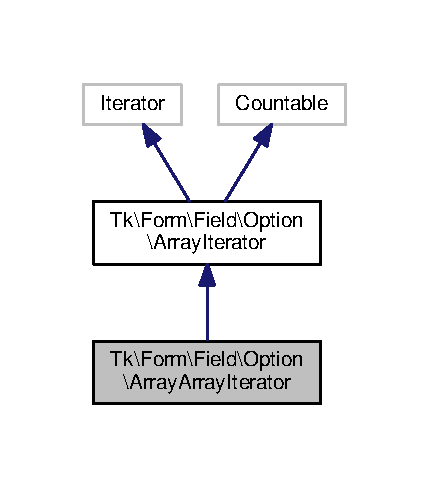
\includegraphics[width=206pt]{classTk_1_1Form_1_1Field_1_1Option_1_1ArrayArrayIterator__inherit__graph}
\end{center}
\end{figure}
\subsection*{Public Member Functions}
\begin{DoxyCompactItemize}
\item 
\hyperlink{classTk_1_1Form_1_1Field_1_1Option_1_1ArrayArrayIterator_a1686519fd5f76a4319498df3c4edc2a2}{\+\_\+\+\_\+construct} (array \$list)
\item 
\hyperlink{classTk_1_1Form_1_1Field_1_1Option_1_1ArrayArrayIterator_aaaf35e9b1163ac62d9d6e4d014b098a4}{current} ()
\end{DoxyCompactItemize}
\subsection*{Additional Inherited Members}


\subsection{Detailed Description}
Use this iterator to create an options list from an array.

$<$?php \$iterator = new \hyperlink{classTk_1_1Form_1_1Field_1_1Option_1_1ArrayArrayIterator}{Array\+Array\+Iterator}(array( array('-- Select --', ''), array('Admin', 'admin', true, 'label'), array('Moderator', 'moderator', false, 'label'), array('User', 'user')) ); ?$>$

Each sub array should contain the following structure\+:

array ( 0 =$>$ 'Text', // \hyperlink{classTk_1_1Form_1_1Field_1_1Option}{Option} Text 1 =$>$ 'Value', // \hyperlink{classTk_1_1Form_1_1Field_1_1Option}{Option} value (optional) 2 =$>$ false, // \hyperlink{classTk_1_1Form_1_1Field_1_1Option}{Option} Disabled value (optional) 3 =$>$ 'label' // \hyperlink{classTk_1_1Form_1_1Field_1_1Option}{Option} Label (optional) )

\begin{DoxyAuthor}{Author}
Michael Mifsud \href{mailto:info@tropotek.com}{\tt info@tropotek.\+com} \hyperlink{}{Copyright 2015 Michael Mifsud }
\end{DoxyAuthor}


\subsection{Constructor \& Destructor Documentation}
\hypertarget{classTk_1_1Form_1_1Field_1_1Option_1_1ArrayArrayIterator_a1686519fd5f76a4319498df3c4edc2a2}{\index{Tk\+::\+Form\+::\+Field\+::\+Option\+::\+Array\+Array\+Iterator@{Tk\+::\+Form\+::\+Field\+::\+Option\+::\+Array\+Array\+Iterator}!\+\_\+\+\_\+construct@{\+\_\+\+\_\+construct}}
\index{\+\_\+\+\_\+construct@{\+\_\+\+\_\+construct}!Tk\+::\+Form\+::\+Field\+::\+Option\+::\+Array\+Array\+Iterator@{Tk\+::\+Form\+::\+Field\+::\+Option\+::\+Array\+Array\+Iterator}}
\subsubsection[{\+\_\+\+\_\+construct}]{\setlength{\rightskip}{0pt plus 5cm}Tk\textbackslash{}\+Form\textbackslash{}\+Field\textbackslash{}\+Option\textbackslash{}\+Array\+Array\+Iterator\+::\+\_\+\+\_\+construct (
\begin{DoxyParamCaption}
\item[{array}]{\$list}
\end{DoxyParamCaption}
)}}\label{classTk_1_1Form_1_1Field_1_1Option_1_1ArrayArrayIterator_a1686519fd5f76a4319498df3c4edc2a2}

\begin{DoxyParams}[1]{Parameters}
array & {\em \$list} & \\
\hline
\end{DoxyParams}


\subsection{Member Function Documentation}
\hypertarget{classTk_1_1Form_1_1Field_1_1Option_1_1ArrayArrayIterator_aaaf35e9b1163ac62d9d6e4d014b098a4}{\index{Tk\+::\+Form\+::\+Field\+::\+Option\+::\+Array\+Array\+Iterator@{Tk\+::\+Form\+::\+Field\+::\+Option\+::\+Array\+Array\+Iterator}!current@{current}}
\index{current@{current}!Tk\+::\+Form\+::\+Field\+::\+Option\+::\+Array\+Array\+Iterator@{Tk\+::\+Form\+::\+Field\+::\+Option\+::\+Array\+Array\+Iterator}}
\subsubsection[{current}]{\setlength{\rightskip}{0pt plus 5cm}Tk\textbackslash{}\+Form\textbackslash{}\+Field\textbackslash{}\+Option\textbackslash{}\+Array\+Array\+Iterator\+::current (
\begin{DoxyParamCaption}
{}
\end{DoxyParamCaption}
)}}\label{classTk_1_1Form_1_1Field_1_1Option_1_1ArrayArrayIterator_aaaf35e9b1163ac62d9d6e4d014b098a4}
Return the current element

\hyperlink{}{mixed Can return any type.  5.\+0.\+0 }

The documentation for this class was generated from the following file\+:\begin{DoxyCompactItemize}
\item 
vendor/ttek/tk-\/form/\+Tk/\+Form/\+Field/\+Option/Array\+Array\+Iterator.\+php\end{DoxyCompactItemize}

\hypertarget{classTk_1_1Form_1_1Field_1_1Option_1_1ArrayIterator}{\section{Tk\textbackslash{}Form\textbackslash{}Field\textbackslash{}Option\textbackslash{}Array\+Iterator Class Reference}
\label{classTk_1_1Form_1_1Field_1_1Option_1_1ArrayIterator}\index{Tk\textbackslash{}\+Form\textbackslash{}\+Field\textbackslash{}\+Option\textbackslash{}\+Array\+Iterator@{Tk\textbackslash{}\+Form\textbackslash{}\+Field\textbackslash{}\+Option\textbackslash{}\+Array\+Iterator}}
}


Inheritance diagram for Tk\textbackslash{}Form\textbackslash{}Field\textbackslash{}Option\textbackslash{}Array\+Iterator\+:\nopagebreak
\begin{figure}[H]
\begin{center}
\leavevmode
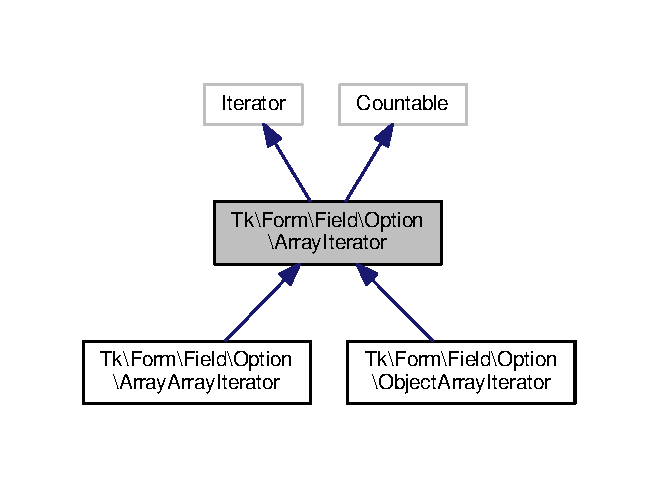
\includegraphics[width=316pt]{classTk_1_1Form_1_1Field_1_1Option_1_1ArrayIterator__inherit__graph}
\end{center}
\end{figure}
\subsection*{Public Member Functions}
\begin{DoxyCompactItemize}
\item 
\hyperlink{classTk_1_1Form_1_1Field_1_1Option_1_1ArrayIterator_ac4fdd09eecbc05317db2dc0131c2016c}{\+\_\+\+\_\+construct} (array \$list)
\item 
\hyperlink{classTk_1_1Form_1_1Field_1_1Option_1_1ArrayIterator_a3209d9d1c8893229fba7239836c4dc9b}{current} ()
\item 
\hyperlink{classTk_1_1Form_1_1Field_1_1Option_1_1ArrayIterator_a51f470ada09d9085a7d9e20aabca27a2}{key} ()
\item 
\hyperlink{classTk_1_1Form_1_1Field_1_1Option_1_1ArrayIterator_a024f4290ec2de05331b6decf20abebb2}{next} ()
\item 
\hyperlink{classTk_1_1Form_1_1Field_1_1Option_1_1ArrayIterator_a2398de5dd7c52d4510490a6e076f6f23}{valid} ()
\item 
\hyperlink{classTk_1_1Form_1_1Field_1_1Option_1_1ArrayIterator_af8194e9aec780f4a0835e40a35c4f9f7}{rewind} ()
\item 
\hyperlink{classTk_1_1Form_1_1Field_1_1Option_1_1ArrayIterator_a111de27b649638fd451454a9ff7ae9b0}{count} ()
\end{DoxyCompactItemize}
\subsection*{Protected Member Functions}
\begin{DoxyCompactItemize}
\item 
\hyperlink{classTk_1_1Form_1_1Field_1_1Option_1_1ArrayIterator_a73d7e5b6561e4d1905cf39bea3e398e0}{get\+Key} (\$i)
\end{DoxyCompactItemize}
\subsection*{Protected Attributes}
\begin{DoxyCompactItemize}
\item 
\hypertarget{classTk_1_1Form_1_1Field_1_1Option_1_1ArrayIterator_affcca538b814f074ae9b520899195299}{{\bfseries \$idx} = 0}\label{classTk_1_1Form_1_1Field_1_1Option_1_1ArrayIterator_affcca538b814f074ae9b520899195299}

\item 
\hypertarget{classTk_1_1Form_1_1Field_1_1Option_1_1ArrayIterator_ad028c6af8d8e66b75fa6a14312b45c49}{{\bfseries \$list} = array()}\label{classTk_1_1Form_1_1Field_1_1Option_1_1ArrayIterator_ad028c6af8d8e66b75fa6a14312b45c49}

\end{DoxyCompactItemize}


\subsection{Detailed Description}
Use this iterator to create an options list from an array.

$<$?php \$iterator = new Option\+Array(array('-- Select --' =$>$ '', 'Admin' =$>$ 'admin', 'Moderator' =$>$ 'moderator', 'User' =$>$ 'user')); ?$>$

\begin{DoxyAuthor}{Author}
Michael Mifsud \href{mailto:info@tropotek.com}{\tt info@tropotek.\+com} \hyperlink{}{Copyright 2015 Michael Mifsud }
\end{DoxyAuthor}


\subsection{Constructor \& Destructor Documentation}
\hypertarget{classTk_1_1Form_1_1Field_1_1Option_1_1ArrayIterator_ac4fdd09eecbc05317db2dc0131c2016c}{\index{Tk\+::\+Form\+::\+Field\+::\+Option\+::\+Array\+Iterator@{Tk\+::\+Form\+::\+Field\+::\+Option\+::\+Array\+Iterator}!\+\_\+\+\_\+construct@{\+\_\+\+\_\+construct}}
\index{\+\_\+\+\_\+construct@{\+\_\+\+\_\+construct}!Tk\+::\+Form\+::\+Field\+::\+Option\+::\+Array\+Iterator@{Tk\+::\+Form\+::\+Field\+::\+Option\+::\+Array\+Iterator}}
\subsubsection[{\+\_\+\+\_\+construct}]{\setlength{\rightskip}{0pt plus 5cm}Tk\textbackslash{}\+Form\textbackslash{}\+Field\textbackslash{}\+Option\textbackslash{}\+Array\+Iterator\+::\+\_\+\+\_\+construct (
\begin{DoxyParamCaption}
\item[{array}]{\$list}
\end{DoxyParamCaption}
)}}\label{classTk_1_1Form_1_1Field_1_1Option_1_1ArrayIterator_ac4fdd09eecbc05317db2dc0131c2016c}

\begin{DoxyParams}[1]{Parameters}
array & {\em \$list} & \\
\hline
\end{DoxyParams}


\subsection{Member Function Documentation}
\hypertarget{classTk_1_1Form_1_1Field_1_1Option_1_1ArrayIterator_a111de27b649638fd451454a9ff7ae9b0}{\index{Tk\+::\+Form\+::\+Field\+::\+Option\+::\+Array\+Iterator@{Tk\+::\+Form\+::\+Field\+::\+Option\+::\+Array\+Iterator}!count@{count}}
\index{count@{count}!Tk\+::\+Form\+::\+Field\+::\+Option\+::\+Array\+Iterator@{Tk\+::\+Form\+::\+Field\+::\+Option\+::\+Array\+Iterator}}
\subsubsection[{count}]{\setlength{\rightskip}{0pt plus 5cm}Tk\textbackslash{}\+Form\textbackslash{}\+Field\textbackslash{}\+Option\textbackslash{}\+Array\+Iterator\+::count (
\begin{DoxyParamCaption}
{}
\end{DoxyParamCaption}
)}}\label{classTk_1_1Form_1_1Field_1_1Option_1_1ArrayIterator_a111de27b649638fd451454a9ff7ae9b0}
Count elements of an object

\hyperlink{}{int The custom count as an integer. } 

The return value is cast to an integer. \begin{DoxySince}{Since}
5.\+1.\+0 
\end{DoxySince}
\hypertarget{classTk_1_1Form_1_1Field_1_1Option_1_1ArrayIterator_a3209d9d1c8893229fba7239836c4dc9b}{\index{Tk\+::\+Form\+::\+Field\+::\+Option\+::\+Array\+Iterator@{Tk\+::\+Form\+::\+Field\+::\+Option\+::\+Array\+Iterator}!current@{current}}
\index{current@{current}!Tk\+::\+Form\+::\+Field\+::\+Option\+::\+Array\+Iterator@{Tk\+::\+Form\+::\+Field\+::\+Option\+::\+Array\+Iterator}}
\subsubsection[{current}]{\setlength{\rightskip}{0pt plus 5cm}Tk\textbackslash{}\+Form\textbackslash{}\+Field\textbackslash{}\+Option\textbackslash{}\+Array\+Iterator\+::current (
\begin{DoxyParamCaption}
{}
\end{DoxyParamCaption}
)}}\label{classTk_1_1Form_1_1Field_1_1Option_1_1ArrayIterator_a3209d9d1c8893229fba7239836c4dc9b}
Return the current element

\hyperlink{}{mixed Can return any type.  5.\+0.\+0 }\hypertarget{classTk_1_1Form_1_1Field_1_1Option_1_1ArrayIterator_a73d7e5b6561e4d1905cf39bea3e398e0}{\index{Tk\+::\+Form\+::\+Field\+::\+Option\+::\+Array\+Iterator@{Tk\+::\+Form\+::\+Field\+::\+Option\+::\+Array\+Iterator}!get\+Key@{get\+Key}}
\index{get\+Key@{get\+Key}!Tk\+::\+Form\+::\+Field\+::\+Option\+::\+Array\+Iterator@{Tk\+::\+Form\+::\+Field\+::\+Option\+::\+Array\+Iterator}}
\subsubsection[{get\+Key}]{\setlength{\rightskip}{0pt plus 5cm}Tk\textbackslash{}\+Form\textbackslash{}\+Field\textbackslash{}\+Option\textbackslash{}\+Array\+Iterator\+::get\+Key (
\begin{DoxyParamCaption}
\item[{}]{\$i}
\end{DoxyParamCaption}
)\hspace{0.3cm}{\ttfamily [protected]}}}\label{classTk_1_1Form_1_1Field_1_1Option_1_1ArrayIterator_a73d7e5b6561e4d1905cf39bea3e398e0}
get\+Key


\begin{DoxyParams}{Parameters}
{\em \$i} & \\
\hline
\end{DoxyParams}
\begin{DoxyReturn}{Returns}
mixed 
\end{DoxyReturn}
\hypertarget{classTk_1_1Form_1_1Field_1_1Option_1_1ArrayIterator_a51f470ada09d9085a7d9e20aabca27a2}{\index{Tk\+::\+Form\+::\+Field\+::\+Option\+::\+Array\+Iterator@{Tk\+::\+Form\+::\+Field\+::\+Option\+::\+Array\+Iterator}!key@{key}}
\index{key@{key}!Tk\+::\+Form\+::\+Field\+::\+Option\+::\+Array\+Iterator@{Tk\+::\+Form\+::\+Field\+::\+Option\+::\+Array\+Iterator}}
\subsubsection[{key}]{\setlength{\rightskip}{0pt plus 5cm}Tk\textbackslash{}\+Form\textbackslash{}\+Field\textbackslash{}\+Option\textbackslash{}\+Array\+Iterator\+::key (
\begin{DoxyParamCaption}
{}
\end{DoxyParamCaption}
)}}\label{classTk_1_1Form_1_1Field_1_1Option_1_1ArrayIterator_a51f470ada09d9085a7d9e20aabca27a2}
Return the key of the current element

\hyperlink{}{mixed scalar on success, or null on failure.  5.\+0.\+0 }\hypertarget{classTk_1_1Form_1_1Field_1_1Option_1_1ArrayIterator_a024f4290ec2de05331b6decf20abebb2}{\index{Tk\+::\+Form\+::\+Field\+::\+Option\+::\+Array\+Iterator@{Tk\+::\+Form\+::\+Field\+::\+Option\+::\+Array\+Iterator}!next@{next}}
\index{next@{next}!Tk\+::\+Form\+::\+Field\+::\+Option\+::\+Array\+Iterator@{Tk\+::\+Form\+::\+Field\+::\+Option\+::\+Array\+Iterator}}
\subsubsection[{next}]{\setlength{\rightskip}{0pt plus 5cm}Tk\textbackslash{}\+Form\textbackslash{}\+Field\textbackslash{}\+Option\textbackslash{}\+Array\+Iterator\+::next (
\begin{DoxyParamCaption}
{}
\end{DoxyParamCaption}
)}}\label{classTk_1_1Form_1_1Field_1_1Option_1_1ArrayIterator_a024f4290ec2de05331b6decf20abebb2}
Move forward to next element

\hyperlink{}{void Any returned value is ignored.  5.\+0.\+0 }\hypertarget{classTk_1_1Form_1_1Field_1_1Option_1_1ArrayIterator_af8194e9aec780f4a0835e40a35c4f9f7}{\index{Tk\+::\+Form\+::\+Field\+::\+Option\+::\+Array\+Iterator@{Tk\+::\+Form\+::\+Field\+::\+Option\+::\+Array\+Iterator}!rewind@{rewind}}
\index{rewind@{rewind}!Tk\+::\+Form\+::\+Field\+::\+Option\+::\+Array\+Iterator@{Tk\+::\+Form\+::\+Field\+::\+Option\+::\+Array\+Iterator}}
\subsubsection[{rewind}]{\setlength{\rightskip}{0pt plus 5cm}Tk\textbackslash{}\+Form\textbackslash{}\+Field\textbackslash{}\+Option\textbackslash{}\+Array\+Iterator\+::rewind (
\begin{DoxyParamCaption}
{}
\end{DoxyParamCaption}
)}}\label{classTk_1_1Form_1_1Field_1_1Option_1_1ArrayIterator_af8194e9aec780f4a0835e40a35c4f9f7}
Rewind the Iterator to the first element

\hyperlink{}{void Any returned value is ignored.  5.\+0.\+0 }\hypertarget{classTk_1_1Form_1_1Field_1_1Option_1_1ArrayIterator_a2398de5dd7c52d4510490a6e076f6f23}{\index{Tk\+::\+Form\+::\+Field\+::\+Option\+::\+Array\+Iterator@{Tk\+::\+Form\+::\+Field\+::\+Option\+::\+Array\+Iterator}!valid@{valid}}
\index{valid@{valid}!Tk\+::\+Form\+::\+Field\+::\+Option\+::\+Array\+Iterator@{Tk\+::\+Form\+::\+Field\+::\+Option\+::\+Array\+Iterator}}
\subsubsection[{valid}]{\setlength{\rightskip}{0pt plus 5cm}Tk\textbackslash{}\+Form\textbackslash{}\+Field\textbackslash{}\+Option\textbackslash{}\+Array\+Iterator\+::valid (
\begin{DoxyParamCaption}
{}
\end{DoxyParamCaption}
)}}\label{classTk_1_1Form_1_1Field_1_1Option_1_1ArrayIterator_a2398de5dd7c52d4510490a6e076f6f23}
Checks if current position is valid

\hyperlink{}{boolean The return value will be casted to boolean and then evaluated. Returns true on success or false on failure.  5.\+0.\+0 }

The documentation for this class was generated from the following file\+:\begin{DoxyCompactItemize}
\item 
vendor/ttek/tk-\/form/\+Tk/\+Form/\+Field/\+Option/Array\+Iterator.\+php\end{DoxyCompactItemize}

\hypertarget{classTk_1_1Util_1_1ArrayObject}{\section{Tk\textbackslash{}Util\textbackslash{}Array\+Object Class Reference}
\label{classTk_1_1Util_1_1ArrayObject}\index{Tk\textbackslash{}\+Util\textbackslash{}\+Array\+Object@{Tk\textbackslash{}\+Util\textbackslash{}\+Array\+Object}}
}


Inheritance diagram for Tk\textbackslash{}Util\textbackslash{}Array\+Object\+:\nopagebreak
\begin{figure}[H]
\begin{center}
\leavevmode
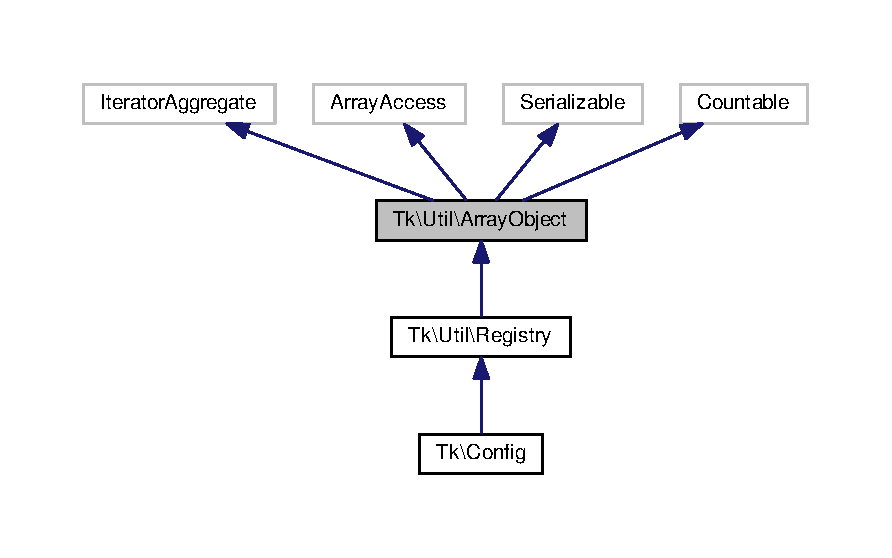
\includegraphics[width=350pt]{classTk_1_1Util_1_1ArrayObject__inherit__graph}
\end{center}
\end{figure}
\subsection*{Public Member Functions}
\begin{DoxyCompactItemize}
\item 
\hyperlink{classTk_1_1Util_1_1ArrayObject_a889d3623fa2dbc6dbc73e35b9c67b538}{\+\_\+\+\_\+construct} (\$array=array())
\item 
\hyperlink{classTk_1_1Util_1_1ArrayObject_ad552b43ac6b610563a7d76d77c935c61}{\+\_\+\+\_\+set} (\$key, \$val)
\item 
\hyperlink{classTk_1_1Util_1_1ArrayObject_aa7e636c8f5f740b101803b582aa080fe}{\+\_\+\+\_\+get} (\$key)
\item 
\hyperlink{classTk_1_1Util_1_1ArrayObject_af07b27b491bf7c31da98586c77c85b27}{get\+Data\+Array} ()
\item 
\hypertarget{classTk_1_1Util_1_1ArrayObject_a02088386acfd52543e241b2ea4e2fad8}{{\bfseries set\+Data\+Array} (\$array)}\label{classTk_1_1Util_1_1ArrayObject_a02088386acfd52543e241b2ea4e2fad8}

\item 
\hyperlink{classTk_1_1Util_1_1ArrayObject_afde4b2acc29ad02d0fb87fb360d20d2c}{merge} (\$array)
\item 
\hyperlink{classTk_1_1Util_1_1ArrayObject_a24784b77dfbe5ca2b343f8c2a3029614}{get\+Iterator} ()
\item 
\hyperlink{classTk_1_1Util_1_1ArrayObject_acb1a3d463f815decdab576b03a4dc262}{offset\+Set} (\$offset, \$value)
\item 
\hyperlink{classTk_1_1Util_1_1ArrayObject_a6286851870bdec9355cd8dce9edff6b6}{offset\+Exists} (\$offset)
\item 
\hyperlink{classTk_1_1Util_1_1ArrayObject_ad57a362c3b33ba6e41890cf56fa7697f}{offset\+Unset} (\$offset)
\item 
\hyperlink{classTk_1_1Util_1_1ArrayObject_a6017eafb107be8de0e8ccdb920e04f3c}{offset\+Get} (\$offset)
\item 
\hyperlink{classTk_1_1Util_1_1ArrayObject_a0a0a5c6b36eed7a834d9174fc98eb69d}{serialize} ()
\item 
\hyperlink{classTk_1_1Util_1_1ArrayObject_aa9b0d06d391d1053ac0f582a06073a7b}{unserialize} (\$data)
\item 
\hyperlink{classTk_1_1Util_1_1ArrayObject_a4e8d9b5ea97161a52a6cd90c6ccaf255}{count} ()
\item 
\hyperlink{classTk_1_1Util_1_1ArrayObject_ac5daa15e14f60b51b6457c036796ed4d}{set} (\$key, \$val)
\item 
\hyperlink{classTk_1_1Util_1_1ArrayObject_af6307b4520b9ebf1338affbfc8c4844f}{nset} (\$key, \$val)
\item 
\hyperlink{classTk_1_1Util_1_1ArrayObject_aa3079cb50bd82b253fcded0a3b1f57d5}{get} (\$key)
\item 
\hyperlink{classTk_1_1Util_1_1ArrayObject_aa0524a20e7d99c45c36776bd708da358}{exists} (\$key)
\item 
\hyperlink{classTk_1_1Util_1_1ArrayObject_a2acff7bb427ff2073c7034c9f18f10a9}{delete} (\$key)
\item 
\hyperlink{classTk_1_1Util_1_1ArrayObject_a9466c18c6e4893b2036e07b5508fa453}{to\+String} ()
\item 
\hyperlink{classTk_1_1Util_1_1ArrayObject_a06135715ec8419a3665cd5a3e80c3854}{\+\_\+\+\_\+to\+String} ()
\end{DoxyCompactItemize}


\subsection{Detailed Description}
A wrapper for the php array object

This object also contains all the array functions as methods.

\begin{DoxyAuthor}{Author}
Michael Mifsud \href{mailto:info@tropotek.com}{\tt info@tropotek.\+com} \hyperlink{}{Copyright 2007 Michael Mifsud }
\end{DoxyAuthor}


\subsection{Constructor \& Destructor Documentation}
\hypertarget{classTk_1_1Util_1_1ArrayObject_a889d3623fa2dbc6dbc73e35b9c67b538}{\index{Tk\+::\+Util\+::\+Array\+Object@{Tk\+::\+Util\+::\+Array\+Object}!\+\_\+\+\_\+construct@{\+\_\+\+\_\+construct}}
\index{\+\_\+\+\_\+construct@{\+\_\+\+\_\+construct}!Tk\+::\+Util\+::\+Array\+Object@{Tk\+::\+Util\+::\+Array\+Object}}
\subsubsection[{\+\_\+\+\_\+construct}]{\setlength{\rightskip}{0pt plus 5cm}Tk\textbackslash{}\+Util\textbackslash{}\+Array\+Object\+::\+\_\+\+\_\+construct (
\begin{DoxyParamCaption}
\item[{}]{\$array = {\ttfamily array()}}
\end{DoxyParamCaption}
)}}\label{classTk_1_1Util_1_1ArrayObject_a889d3623fa2dbc6dbc73e35b9c67b538}

\begin{DoxyParams}[1]{Parameters}
array & {\em \$array} & \\
\hline
\end{DoxyParams}


\subsection{Member Function Documentation}
\hypertarget{classTk_1_1Util_1_1ArrayObject_aa7e636c8f5f740b101803b582aa080fe}{\index{Tk\+::\+Util\+::\+Array\+Object@{Tk\+::\+Util\+::\+Array\+Object}!\+\_\+\+\_\+get@{\+\_\+\+\_\+get}}
\index{\+\_\+\+\_\+get@{\+\_\+\+\_\+get}!Tk\+::\+Util\+::\+Array\+Object@{Tk\+::\+Util\+::\+Array\+Object}}
\subsubsection[{\+\_\+\+\_\+get}]{\setlength{\rightskip}{0pt plus 5cm}Tk\textbackslash{}\+Util\textbackslash{}\+Array\+Object\+::\+\_\+\+\_\+get (
\begin{DoxyParamCaption}
\item[{}]{\$key}
\end{DoxyParamCaption}
)}}\label{classTk_1_1Util_1_1ArrayObject_aa7e636c8f5f740b101803b582aa080fe}
Allow for the items to be treated as object params E\+G\+: \$arr\+Obj-\/$>$item = \$arr\+Obj\mbox{[}'item'\mbox{]}


\begin{DoxyParams}[1]{Parameters}
string & {\em \$key} & \\
\hline
\end{DoxyParams}
\begin{DoxyReturn}{Returns}
mixed 
\end{DoxyReturn}
\hypertarget{classTk_1_1Util_1_1ArrayObject_ad552b43ac6b610563a7d76d77c935c61}{\index{Tk\+::\+Util\+::\+Array\+Object@{Tk\+::\+Util\+::\+Array\+Object}!\+\_\+\+\_\+set@{\+\_\+\+\_\+set}}
\index{\+\_\+\+\_\+set@{\+\_\+\+\_\+set}!Tk\+::\+Util\+::\+Array\+Object@{Tk\+::\+Util\+::\+Array\+Object}}
\subsubsection[{\+\_\+\+\_\+set}]{\setlength{\rightskip}{0pt plus 5cm}Tk\textbackslash{}\+Util\textbackslash{}\+Array\+Object\+::\+\_\+\+\_\+set (
\begin{DoxyParamCaption}
\item[{}]{\$key, }
\item[{}]{\$val}
\end{DoxyParamCaption}
)}}\label{classTk_1_1Util_1_1ArrayObject_ad552b43ac6b610563a7d76d77c935c61}
Allow for the items to be treated as object params E\+G\+: \$arr\+Obj-\/$>$item = \$arr\+Obj\mbox{[}'item'\mbox{]}


\begin{DoxyParams}[1]{Parameters}
string & {\em \$key} & \\
\hline
mixed & {\em \$val} & \\
\hline
\end{DoxyParams}
\hypertarget{classTk_1_1Util_1_1ArrayObject_a06135715ec8419a3665cd5a3e80c3854}{\index{Tk\+::\+Util\+::\+Array\+Object@{Tk\+::\+Util\+::\+Array\+Object}!\+\_\+\+\_\+to\+String@{\+\_\+\+\_\+to\+String}}
\index{\+\_\+\+\_\+to\+String@{\+\_\+\+\_\+to\+String}!Tk\+::\+Util\+::\+Array\+Object@{Tk\+::\+Util\+::\+Array\+Object}}
\subsubsection[{\+\_\+\+\_\+to\+String}]{\setlength{\rightskip}{0pt plus 5cm}Tk\textbackslash{}\+Util\textbackslash{}\+Array\+Object\+::\+\_\+\+\_\+to\+String (
\begin{DoxyParamCaption}
{}
\end{DoxyParamCaption}
)}}\label{classTk_1_1Util_1_1ArrayObject_a06135715ec8419a3665cd5a3e80c3854}
\+\_\+\+\_\+to\+String

\begin{DoxyReturn}{Returns}
string 
\end{DoxyReturn}
\hypertarget{classTk_1_1Util_1_1ArrayObject_a4e8d9b5ea97161a52a6cd90c6ccaf255}{\index{Tk\+::\+Util\+::\+Array\+Object@{Tk\+::\+Util\+::\+Array\+Object}!count@{count}}
\index{count@{count}!Tk\+::\+Util\+::\+Array\+Object@{Tk\+::\+Util\+::\+Array\+Object}}
\subsubsection[{count}]{\setlength{\rightskip}{0pt plus 5cm}Tk\textbackslash{}\+Util\textbackslash{}\+Array\+Object\+::count (
\begin{DoxyParamCaption}
{}
\end{DoxyParamCaption}
)}}\label{classTk_1_1Util_1_1ArrayObject_a4e8d9b5ea97161a52a6cd90c6ccaf255}
\$name 

\begin{DoxyReturn}{Returns}
int 
\end{DoxyReturn}
\hypertarget{classTk_1_1Util_1_1ArrayObject_a2acff7bb427ff2073c7034c9f18f10a9}{\index{Tk\+::\+Util\+::\+Array\+Object@{Tk\+::\+Util\+::\+Array\+Object}!delete@{delete}}
\index{delete@{delete}!Tk\+::\+Util\+::\+Array\+Object@{Tk\+::\+Util\+::\+Array\+Object}}
\subsubsection[{delete}]{\setlength{\rightskip}{0pt plus 5cm}Tk\textbackslash{}\+Util\textbackslash{}\+Array\+Object\+::delete (
\begin{DoxyParamCaption}
\item[{}]{\$key}
\end{DoxyParamCaption}
)}}\label{classTk_1_1Util_1_1ArrayObject_a2acff7bb427ff2073c7034c9f18f10a9}
Remove an entry from the registry cache


\begin{DoxyParams}[1]{Parameters}
string & {\em \$key} & \\
\hline
\end{DoxyParams}
\begin{DoxyReturn}{Returns}
\hyperlink{classTk_1_1Util_1_1ArrayObject}{Array\+Object} 
\end{DoxyReturn}
\hypertarget{classTk_1_1Util_1_1ArrayObject_aa0524a20e7d99c45c36776bd708da358}{\index{Tk\+::\+Util\+::\+Array\+Object@{Tk\+::\+Util\+::\+Array\+Object}!exists@{exists}}
\index{exists@{exists}!Tk\+::\+Util\+::\+Array\+Object@{Tk\+::\+Util\+::\+Array\+Object}}
\subsubsection[{exists}]{\setlength{\rightskip}{0pt plus 5cm}Tk\textbackslash{}\+Util\textbackslash{}\+Array\+Object\+::exists (
\begin{DoxyParamCaption}
\item[{}]{\$key}
\end{DoxyParamCaption}
)}}\label{classTk_1_1Util_1_1ArrayObject_aa0524a20e7d99c45c36776bd708da358}
Test if an array key exists in this object


\begin{DoxyParams}[1]{Parameters}
string & {\em \$key} & \\
\hline
\end{DoxyParams}
\begin{DoxyReturn}{Returns}
bool 
\end{DoxyReturn}
\hypertarget{classTk_1_1Util_1_1ArrayObject_aa3079cb50bd82b253fcded0a3b1f57d5}{\index{Tk\+::\+Util\+::\+Array\+Object@{Tk\+::\+Util\+::\+Array\+Object}!get@{get}}
\index{get@{get}!Tk\+::\+Util\+::\+Array\+Object@{Tk\+::\+Util\+::\+Array\+Object}}
\subsubsection[{get}]{\setlength{\rightskip}{0pt plus 5cm}Tk\textbackslash{}\+Util\textbackslash{}\+Array\+Object\+::get (
\begin{DoxyParamCaption}
\item[{}]{\$key}
\end{DoxyParamCaption}
)}}\label{classTk_1_1Util_1_1ArrayObject_aa3079cb50bd82b253fcded0a3b1f57d5}
Allow for the items to be treated as object params E\+G\+: \$arr\+Obj-\/$>$item = \$arr\+Obj\mbox{[}'item'\mbox{]}


\begin{DoxyParams}[1]{Parameters}
string & {\em \$key} & \\
\hline
\end{DoxyParams}
\begin{DoxyReturn}{Returns}
mixed 
\end{DoxyReturn}
\hypertarget{classTk_1_1Util_1_1ArrayObject_af07b27b491bf7c31da98586c77c85b27}{\index{Tk\+::\+Util\+::\+Array\+Object@{Tk\+::\+Util\+::\+Array\+Object}!get\+Data\+Array@{get\+Data\+Array}}
\index{get\+Data\+Array@{get\+Data\+Array}!Tk\+::\+Util\+::\+Array\+Object@{Tk\+::\+Util\+::\+Array\+Object}}
\subsubsection[{get\+Data\+Array}]{\setlength{\rightskip}{0pt plus 5cm}Tk\textbackslash{}\+Util\textbackslash{}\+Array\+Object\+::get\+Data\+Array (
\begin{DoxyParamCaption}
{}
\end{DoxyParamCaption}
)}}\label{classTk_1_1Util_1_1ArrayObject_af07b27b491bf7c31da98586c77c85b27}
Return the native data array

\begin{DoxyReturn}{Returns}
array 
\end{DoxyReturn}
\hypertarget{classTk_1_1Util_1_1ArrayObject_a24784b77dfbe5ca2b343f8c2a3029614}{\index{Tk\+::\+Util\+::\+Array\+Object@{Tk\+::\+Util\+::\+Array\+Object}!get\+Iterator@{get\+Iterator}}
\index{get\+Iterator@{get\+Iterator}!Tk\+::\+Util\+::\+Array\+Object@{Tk\+::\+Util\+::\+Array\+Object}}
\subsubsection[{get\+Iterator}]{\setlength{\rightskip}{0pt plus 5cm}Tk\textbackslash{}\+Util\textbackslash{}\+Array\+Object\+::get\+Iterator (
\begin{DoxyParamCaption}
{}
\end{DoxyParamCaption}
)}}\label{classTk_1_1Util_1_1ArrayObject_a24784b77dfbe5ca2b343f8c2a3029614}
\begin{DoxyReturn}{Returns}

\end{DoxyReturn}
\hypertarget{classTk_1_1Util_1_1ArrayObject_afde4b2acc29ad02d0fb87fb360d20d2c}{\index{Tk\+::\+Util\+::\+Array\+Object@{Tk\+::\+Util\+::\+Array\+Object}!merge@{merge}}
\index{merge@{merge}!Tk\+::\+Util\+::\+Array\+Object@{Tk\+::\+Util\+::\+Array\+Object}}
\subsubsection[{merge}]{\setlength{\rightskip}{0pt plus 5cm}Tk\textbackslash{}\+Util\textbackslash{}\+Array\+Object\+::merge (
\begin{DoxyParamCaption}
\item[{}]{\$array}
\end{DoxyParamCaption}
)}}\label{classTk_1_1Util_1_1ArrayObject_afde4b2acc29ad02d0fb87fb360d20d2c}
merge an external array into this array


\begin{DoxyParams}[1]{Parameters}
array & {\em \$array} & \\
\hline
\end{DoxyParams}
\begin{DoxyReturn}{Returns}
\hyperlink{classTk_1_1Util_1_1ArrayObject}{Array\+Object} 
\end{DoxyReturn}
\hypertarget{classTk_1_1Util_1_1ArrayObject_af6307b4520b9ebf1338affbfc8c4844f}{\index{Tk\+::\+Util\+::\+Array\+Object@{Tk\+::\+Util\+::\+Array\+Object}!nset@{nset}}
\index{nset@{nset}!Tk\+::\+Util\+::\+Array\+Object@{Tk\+::\+Util\+::\+Array\+Object}}
\subsubsection[{nset}]{\setlength{\rightskip}{0pt plus 5cm}Tk\textbackslash{}\+Util\textbackslash{}\+Array\+Object\+::nset (
\begin{DoxyParamCaption}
\item[{}]{\$key, }
\item[{}]{\$val}
\end{DoxyParamCaption}
)}}\label{classTk_1_1Util_1_1ArrayObject_af6307b4520b9ebf1338affbfc8c4844f}
Set an entry into the registry cache if not exist


\begin{DoxyParams}[1]{Parameters}
string & {\em \$key} & \\
\hline
mixed & {\em \$val} & \\
\hline
\end{DoxyParams}
\begin{DoxyReturn}{Returns}
\hyperlink{classTk_1_1Util_1_1ArrayObject}{Array\+Object} 
\end{DoxyReturn}
\hypertarget{classTk_1_1Util_1_1ArrayObject_a6286851870bdec9355cd8dce9edff6b6}{\index{Tk\+::\+Util\+::\+Array\+Object@{Tk\+::\+Util\+::\+Array\+Object}!offset\+Exists@{offset\+Exists}}
\index{offset\+Exists@{offset\+Exists}!Tk\+::\+Util\+::\+Array\+Object@{Tk\+::\+Util\+::\+Array\+Object}}
\subsubsection[{offset\+Exists}]{\setlength{\rightskip}{0pt plus 5cm}Tk\textbackslash{}\+Util\textbackslash{}\+Array\+Object\+::offset\+Exists (
\begin{DoxyParamCaption}
\item[{}]{\$offset}
\end{DoxyParamCaption}
)}}\label{classTk_1_1Util_1_1ArrayObject_a6286851870bdec9355cd8dce9edff6b6}

\begin{DoxyParams}[1]{Parameters}
string & {\em \$offset} & \\
\hline
\end{DoxyParams}
\begin{DoxyReturn}{Returns}
bool 
\end{DoxyReturn}
\hypertarget{classTk_1_1Util_1_1ArrayObject_a6017eafb107be8de0e8ccdb920e04f3c}{\index{Tk\+::\+Util\+::\+Array\+Object@{Tk\+::\+Util\+::\+Array\+Object}!offset\+Get@{offset\+Get}}
\index{offset\+Get@{offset\+Get}!Tk\+::\+Util\+::\+Array\+Object@{Tk\+::\+Util\+::\+Array\+Object}}
\subsubsection[{offset\+Get}]{\setlength{\rightskip}{0pt plus 5cm}Tk\textbackslash{}\+Util\textbackslash{}\+Array\+Object\+::offset\+Get (
\begin{DoxyParamCaption}
\item[{}]{\$offset}
\end{DoxyParamCaption}
)}}\label{classTk_1_1Util_1_1ArrayObject_a6017eafb107be8de0e8ccdb920e04f3c}

\begin{DoxyParams}[1]{Parameters}
string & {\em \$offset} & \\
\hline
\end{DoxyParams}
\begin{DoxyReturn}{Returns}
bool 
\end{DoxyReturn}
\hypertarget{classTk_1_1Util_1_1ArrayObject_acb1a3d463f815decdab576b03a4dc262}{\index{Tk\+::\+Util\+::\+Array\+Object@{Tk\+::\+Util\+::\+Array\+Object}!offset\+Set@{offset\+Set}}
\index{offset\+Set@{offset\+Set}!Tk\+::\+Util\+::\+Array\+Object@{Tk\+::\+Util\+::\+Array\+Object}}
\subsubsection[{offset\+Set}]{\setlength{\rightskip}{0pt plus 5cm}Tk\textbackslash{}\+Util\textbackslash{}\+Array\+Object\+::offset\+Set (
\begin{DoxyParamCaption}
\item[{}]{\$offset, }
\item[{}]{\$value}
\end{DoxyParamCaption}
)}}\label{classTk_1_1Util_1_1ArrayObject_acb1a3d463f815decdab576b03a4dc262}

\begin{DoxyParams}[1]{Parameters}
string & {\em \$offset} & \\
\hline
mixed & {\em \$value} & \\
\hline
\end{DoxyParams}
\hypertarget{classTk_1_1Util_1_1ArrayObject_ad57a362c3b33ba6e41890cf56fa7697f}{\index{Tk\+::\+Util\+::\+Array\+Object@{Tk\+::\+Util\+::\+Array\+Object}!offset\+Unset@{offset\+Unset}}
\index{offset\+Unset@{offset\+Unset}!Tk\+::\+Util\+::\+Array\+Object@{Tk\+::\+Util\+::\+Array\+Object}}
\subsubsection[{offset\+Unset}]{\setlength{\rightskip}{0pt plus 5cm}Tk\textbackslash{}\+Util\textbackslash{}\+Array\+Object\+::offset\+Unset (
\begin{DoxyParamCaption}
\item[{}]{\$offset}
\end{DoxyParamCaption}
)}}\label{classTk_1_1Util_1_1ArrayObject_ad57a362c3b33ba6e41890cf56fa7697f}

\begin{DoxyParams}[1]{Parameters}
string & {\em \$offset} & \\
\hline
\end{DoxyParams}
\hypertarget{classTk_1_1Util_1_1ArrayObject_a0a0a5c6b36eed7a834d9174fc98eb69d}{\index{Tk\+::\+Util\+::\+Array\+Object@{Tk\+::\+Util\+::\+Array\+Object}!serialize@{serialize}}
\index{serialize@{serialize}!Tk\+::\+Util\+::\+Array\+Object@{Tk\+::\+Util\+::\+Array\+Object}}
\subsubsection[{serialize}]{\setlength{\rightskip}{0pt plus 5cm}Tk\textbackslash{}\+Util\textbackslash{}\+Array\+Object\+::serialize (
\begin{DoxyParamCaption}
{}
\end{DoxyParamCaption}
)}}\label{classTk_1_1Util_1_1ArrayObject_a0a0a5c6b36eed7a834d9174fc98eb69d}
\begin{DoxyReturn}{Returns}
string 
\end{DoxyReturn}
\hypertarget{classTk_1_1Util_1_1ArrayObject_ac5daa15e14f60b51b6457c036796ed4d}{\index{Tk\+::\+Util\+::\+Array\+Object@{Tk\+::\+Util\+::\+Array\+Object}!set@{set}}
\index{set@{set}!Tk\+::\+Util\+::\+Array\+Object@{Tk\+::\+Util\+::\+Array\+Object}}
\subsubsection[{set}]{\setlength{\rightskip}{0pt plus 5cm}Tk\textbackslash{}\+Util\textbackslash{}\+Array\+Object\+::set (
\begin{DoxyParamCaption}
\item[{}]{\$key, }
\item[{}]{\$val}
\end{DoxyParamCaption}
)}}\label{classTk_1_1Util_1_1ArrayObject_ac5daa15e14f60b51b6457c036796ed4d}
Allow for the items to be treated as object params E\+G\+: \$arr\+Obj-\/$>$item = \$arr\+Obj\mbox{[}'item'\mbox{]}


\begin{DoxyParams}[1]{Parameters}
 & {\em \$key} & \\
\hline
mixed & {\em \$val} & \\
\hline
\end{DoxyParams}
\begin{DoxyReturn}{Returns}
\hyperlink{classTk_1_1Util_1_1ArrayObject}{Array\+Object} 
\end{DoxyReturn}
\hypertarget{classTk_1_1Util_1_1ArrayObject_a9466c18c6e4893b2036e07b5508fa453}{\index{Tk\+::\+Util\+::\+Array\+Object@{Tk\+::\+Util\+::\+Array\+Object}!to\+String@{to\+String}}
\index{to\+String@{to\+String}!Tk\+::\+Util\+::\+Array\+Object@{Tk\+::\+Util\+::\+Array\+Object}}
\subsubsection[{to\+String}]{\setlength{\rightskip}{0pt plus 5cm}Tk\textbackslash{}\+Util\textbackslash{}\+Array\+Object\+::to\+String (
\begin{DoxyParamCaption}
{}
\end{DoxyParamCaption}
)}}\label{classTk_1_1Util_1_1ArrayObject_a9466c18c6e4893b2036e07b5508fa453}
to\+String

\begin{DoxyReturn}{Returns}
string 
\end{DoxyReturn}
\hypertarget{classTk_1_1Util_1_1ArrayObject_aa9b0d06d391d1053ac0f582a06073a7b}{\index{Tk\+::\+Util\+::\+Array\+Object@{Tk\+::\+Util\+::\+Array\+Object}!unserialize@{unserialize}}
\index{unserialize@{unserialize}!Tk\+::\+Util\+::\+Array\+Object@{Tk\+::\+Util\+::\+Array\+Object}}
\subsubsection[{unserialize}]{\setlength{\rightskip}{0pt plus 5cm}Tk\textbackslash{}\+Util\textbackslash{}\+Array\+Object\+::unserialize (
\begin{DoxyParamCaption}
\item[{}]{\$data}
\end{DoxyParamCaption}
)}}\label{classTk_1_1Util_1_1ArrayObject_aa9b0d06d391d1053ac0f582a06073a7b}

\begin{DoxyParams}[1]{Parameters}
string & {\em \$data} & \\
\hline
\end{DoxyParams}


The documentation for this class was generated from the following file\+:\begin{DoxyCompactItemize}
\item 
vendor/ttek/tk-\/framework/\+Tk/\+Util/Array\+Object.\+php\end{DoxyCompactItemize}

\hypertarget{classTk_1_1Db_1_1ArrayObject}{\section{Tk\textbackslash{}Db\textbackslash{}Array\+Object Class Reference}
\label{classTk_1_1Db_1_1ArrayObject}\index{Tk\textbackslash{}\+Db\textbackslash{}\+Array\+Object@{Tk\textbackslash{}\+Db\textbackslash{}\+Array\+Object}}
}


Inheritance diagram for Tk\textbackslash{}Db\textbackslash{}Array\+Object\+:\nopagebreak
\begin{figure}[H]
\begin{center}
\leavevmode
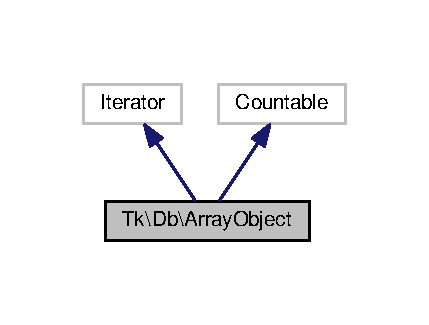
\includegraphics[width=206pt]{classTk_1_1Db_1_1ArrayObject__inherit__graph}
\end{center}
\end{figure}
\subsection*{Public Member Functions}
\begin{DoxyCompactItemize}
\item 
\hyperlink{classTk_1_1Db_1_1ArrayObject_abb0f4cf0e5b67ab269ec531ec0f4b26c}{\+\_\+\+\_\+construct} (\$rows)
\item 
\hyperlink{classTk_1_1Db_1_1ArrayObject_adece20b9b06bd2e72c3f756259727b4a}{\+\_\+\+\_\+destruct} ()
\item 
\hyperlink{classTk_1_1Db_1_1ArrayObject_a5d30be86a7f084af08ce394654420f1b}{get\+Tool} ()
\item 
\hyperlink{classTk_1_1Db_1_1ArrayObject_a39299215dd91c18be56088c37261ecbc}{get\+Mapper} ()
\item 
\hyperlink{classTk_1_1Db_1_1ArrayObject_ad9c2480c061101367b269b3b8411baca}{get\+Statement} ()
\item 
\hyperlink{classTk_1_1Db_1_1ArrayObject_ae3cb9c19eba638907ae6169ead2b2866}{get\+Rows} ()
\item 
\hyperlink{classTk_1_1Db_1_1ArrayObject_a0eb1a07df69e059c358046d9e65e386e}{get} (\$i)
\item 
\hyperlink{classTk_1_1Db_1_1ArrayObject_a7c9e49dde3edbc0bcb397732e7a8176a}{get\+Found\+Rows} ()
\item 
\hyperlink{classTk_1_1Db_1_1ArrayObject_a94b25c0762acb86915e91ff57b01ec61}{rewind} ()
\item 
\hyperlink{classTk_1_1Db_1_1ArrayObject_a3df0c0080e7647b730ae5b5cd102e0d9}{current} ()
\item 
\hyperlink{classTk_1_1Db_1_1ArrayObject_aa73eabffe8c021aa12509c83cf8ddc12}{next} ()
\item 
\hyperlink{classTk_1_1Db_1_1ArrayObject_a41cfb3c1f8c6f9cf2d7ea1d6244157e4}{key} ()
\item 
\hyperlink{classTk_1_1Db_1_1ArrayObject_ad7d1f285d9becc3d71eaa05e9121cb89}{valid} ()
\item 
\hyperlink{classTk_1_1Db_1_1ArrayObject_a62c881bb4e5e4c5067095dc036f124bc}{count} ()
\end{DoxyCompactItemize}
\subsection*{Static Public Member Functions}
\begin{DoxyCompactItemize}
\item 
static \hyperlink{classTk_1_1Db_1_1ArrayObject_acef9db6fcfae6404ac3b318b186e407d}{create\+From\+Mapper} (\hyperlink{classTk_1_1Db_1_1Mapper}{Mapper} \$mapper, \hyperlink{classTk_1_1Db_1_1PdoStatement}{Pdo\+Statement} \$statement, \$tool=null)
\end{DoxyCompactItemize}
\subsection*{Protected Attributes}
\begin{DoxyCompactItemize}
\item 
\hypertarget{classTk_1_1Db_1_1ArrayObject_af34f0e32e8e258554cee2574f05f71cd}{{\bfseries \$mapper} = null}\label{classTk_1_1Db_1_1ArrayObject_af34f0e32e8e258554cee2574f05f71cd}

\item 
\hypertarget{classTk_1_1Db_1_1ArrayObject_ae0e5c4143c950ee15d4d71a215089daa}{{\bfseries \$statement} = null}\label{classTk_1_1Db_1_1ArrayObject_ae0e5c4143c950ee15d4d71a215089daa}

\item 
\hypertarget{classTk_1_1Db_1_1ArrayObject_a053759767d3a0d795b9be97a520194dd}{{\bfseries \$rows} = null}\label{classTk_1_1Db_1_1ArrayObject_a053759767d3a0d795b9be97a520194dd}

\item 
\hypertarget{classTk_1_1Db_1_1ArrayObject_a6ea5aeca879078a9367ed16b81a91312}{{\bfseries \$idx} = 0}\label{classTk_1_1Db_1_1ArrayObject_a6ea5aeca879078a9367ed16b81a91312}

\item 
\hypertarget{classTk_1_1Db_1_1ArrayObject_a299522a9e2fc68d61957b4b42307c365}{{\bfseries \$found\+Rows} = 0}\label{classTk_1_1Db_1_1ArrayObject_a299522a9e2fc68d61957b4b42307c365}

\item 
\hypertarget{classTk_1_1Db_1_1ArrayObject_a6e532f879502d308524dcda1dc24516b}{{\bfseries \$tool} = null}\label{classTk_1_1Db_1_1ArrayObject_a6e532f879502d308524dcda1dc24516b}

\end{DoxyCompactItemize}


\subsection{Detailed Description}
This objected is essentially a wrapper around the \hyperlink{classTk_1_1Db_1_1PdoStatement}{Pdo\+Statement} object with added features such as holding the \hyperlink{classTk_1_1Db_1_1Model}{Model} \hyperlink{classTk_1_1Db_1_1Mapper}{Mapper}, and Db objects.

It automatially maps an obects data if the \hyperlink{classTk_1_1Db_1_1Model}{Model} has the magic methods available

\begin{DoxyAuthor}{Author}
Michael Mifsud \href{mailto:info@tropotek.com}{\tt info@tropotek.\+com} \hyperlink{}{Copyright 2015 Michael Mifsud }
\end{DoxyAuthor}


\subsection{Constructor \& Destructor Documentation}
\hypertarget{classTk_1_1Db_1_1ArrayObject_abb0f4cf0e5b67ab269ec531ec0f4b26c}{\index{Tk\+::\+Db\+::\+Array\+Object@{Tk\+::\+Db\+::\+Array\+Object}!\+\_\+\+\_\+construct@{\+\_\+\+\_\+construct}}
\index{\+\_\+\+\_\+construct@{\+\_\+\+\_\+construct}!Tk\+::\+Db\+::\+Array\+Object@{Tk\+::\+Db\+::\+Array\+Object}}
\subsubsection[{\+\_\+\+\_\+construct}]{\setlength{\rightskip}{0pt plus 5cm}Tk\textbackslash{}\+Db\textbackslash{}\+Array\+Object\+::\+\_\+\+\_\+construct (
\begin{DoxyParamCaption}
\item[{}]{\$rows}
\end{DoxyParamCaption}
)}}\label{classTk_1_1Db_1_1ArrayObject_abb0f4cf0e5b67ab269ec531ec0f4b26c}
Create a D\+B array list object


\begin{DoxyParams}[1]{Parameters}
array & {\em \$rows} & \\
\hline
\end{DoxyParams}
\hypertarget{classTk_1_1Db_1_1ArrayObject_adece20b9b06bd2e72c3f756259727b4a}{\index{Tk\+::\+Db\+::\+Array\+Object@{Tk\+::\+Db\+::\+Array\+Object}!\+\_\+\+\_\+destruct@{\+\_\+\+\_\+destruct}}
\index{\+\_\+\+\_\+destruct@{\+\_\+\+\_\+destruct}!Tk\+::\+Db\+::\+Array\+Object@{Tk\+::\+Db\+::\+Array\+Object}}
\subsubsection[{\+\_\+\+\_\+destruct}]{\setlength{\rightskip}{0pt plus 5cm}Tk\textbackslash{}\+Db\textbackslash{}\+Array\+Object\+::\+\_\+\+\_\+destruct (
\begin{DoxyParamCaption}
{}
\end{DoxyParamCaption}
)}}\label{classTk_1_1Db_1_1ArrayObject_adece20b9b06bd2e72c3f756259727b4a}
Destructor 

\subsection{Member Function Documentation}
\hypertarget{classTk_1_1Db_1_1ArrayObject_a62c881bb4e5e4c5067095dc036f124bc}{\index{Tk\+::\+Db\+::\+Array\+Object@{Tk\+::\+Db\+::\+Array\+Object}!count@{count}}
\index{count@{count}!Tk\+::\+Db\+::\+Array\+Object@{Tk\+::\+Db\+::\+Array\+Object}}
\subsubsection[{count}]{\setlength{\rightskip}{0pt plus 5cm}Tk\textbackslash{}\+Db\textbackslash{}\+Array\+Object\+::count (
\begin{DoxyParamCaption}
{}
\end{DoxyParamCaption}
)}}\label{classTk_1_1Db_1_1ArrayObject_a62c881bb4e5e4c5067095dc036f124bc}
Count

\begin{DoxyReturn}{Returns}
int 
\end{DoxyReturn}
\hypertarget{classTk_1_1Db_1_1ArrayObject_acef9db6fcfae6404ac3b318b186e407d}{\index{Tk\+::\+Db\+::\+Array\+Object@{Tk\+::\+Db\+::\+Array\+Object}!create\+From\+Mapper@{create\+From\+Mapper}}
\index{create\+From\+Mapper@{create\+From\+Mapper}!Tk\+::\+Db\+::\+Array\+Object@{Tk\+::\+Db\+::\+Array\+Object}}
\subsubsection[{create\+From\+Mapper}]{\setlength{\rightskip}{0pt plus 5cm}static Tk\textbackslash{}\+Db\textbackslash{}\+Array\+Object\+::create\+From\+Mapper (
\begin{DoxyParamCaption}
\item[{{\bf Mapper}}]{\$mapper, }
\item[{{\bf Pdo\+Statement}}]{\$statement, }
\item[{}]{\$tool = {\ttfamily null}}
\end{DoxyParamCaption}
)\hspace{0.3cm}{\ttfamily [static]}}}\label{classTk_1_1Db_1_1ArrayObject_acef9db6fcfae6404ac3b318b186e407d}

\begin{DoxyParams}[1]{Parameters}
\hyperlink{classTk_1_1Db_1_1Mapper}{Mapper} & {\em \$mapper} & \\
\hline
\hyperlink{classTk_1_1Db_1_1PdoStatement}{Pdo\+Statement} & {\em \$statement} & \\
\hline
\hyperlink{classTk_1_1Db_1_1Tool}{Tool} & {\em \$tool} & \\
\hline
\end{DoxyParams}
\begin{DoxyReturn}{Returns}
\hyperlink{classTk_1_1Db_1_1ArrayObject}{Array\+Object} 
\end{DoxyReturn}
\hypertarget{classTk_1_1Db_1_1ArrayObject_a3df0c0080e7647b730ae5b5cd102e0d9}{\index{Tk\+::\+Db\+::\+Array\+Object@{Tk\+::\+Db\+::\+Array\+Object}!current@{current}}
\index{current@{current}!Tk\+::\+Db\+::\+Array\+Object@{Tk\+::\+Db\+::\+Array\+Object}}
\subsubsection[{current}]{\setlength{\rightskip}{0pt plus 5cm}Tk\textbackslash{}\+Db\textbackslash{}\+Array\+Object\+::current (
\begin{DoxyParamCaption}
{}
\end{DoxyParamCaption}
)}}\label{classTk_1_1Db_1_1ArrayObject_a3df0c0080e7647b730ae5b5cd102e0d9}
Return the element at the current index

\begin{DoxyReturn}{Returns}
\hyperlink{classTk_1_1Db_1_1Model}{Model} 
\end{DoxyReturn}
\hypertarget{classTk_1_1Db_1_1ArrayObject_a0eb1a07df69e059c358046d9e65e386e}{\index{Tk\+::\+Db\+::\+Array\+Object@{Tk\+::\+Db\+::\+Array\+Object}!get@{get}}
\index{get@{get}!Tk\+::\+Db\+::\+Array\+Object@{Tk\+::\+Db\+::\+Array\+Object}}
\subsubsection[{get}]{\setlength{\rightskip}{0pt plus 5cm}Tk\textbackslash{}\+Db\textbackslash{}\+Array\+Object\+::get (
\begin{DoxyParamCaption}
\item[{}]{\$i}
\end{DoxyParamCaption}
)}}\label{classTk_1_1Db_1_1ArrayObject_a0eb1a07df69e059c358046d9e65e386e}

\begin{DoxyParams}[1]{Parameters}
int & {\em \$i} & \\
\hline
\end{DoxyParams}
\begin{DoxyReturn}{Returns}
Model$\vert$array$\vert$null 
\end{DoxyReturn}
\hypertarget{classTk_1_1Db_1_1ArrayObject_a7c9e49dde3edbc0bcb397732e7a8176a}{\index{Tk\+::\+Db\+::\+Array\+Object@{Tk\+::\+Db\+::\+Array\+Object}!get\+Found\+Rows@{get\+Found\+Rows}}
\index{get\+Found\+Rows@{get\+Found\+Rows}!Tk\+::\+Db\+::\+Array\+Object@{Tk\+::\+Db\+::\+Array\+Object}}
\subsubsection[{get\+Found\+Rows}]{\setlength{\rightskip}{0pt plus 5cm}Tk\textbackslash{}\+Db\textbackslash{}\+Array\+Object\+::get\+Found\+Rows (
\begin{DoxyParamCaption}
{}
\end{DoxyParamCaption}
)}}\label{classTk_1_1Db_1_1ArrayObject_a7c9e49dde3edbc0bcb397732e7a8176a}
Get the total rows available count.

This value will be the available count without a limit.

\begin{DoxyReturn}{Returns}
int 
\end{DoxyReturn}
\hypertarget{classTk_1_1Db_1_1ArrayObject_a39299215dd91c18be56088c37261ecbc}{\index{Tk\+::\+Db\+::\+Array\+Object@{Tk\+::\+Db\+::\+Array\+Object}!get\+Mapper@{get\+Mapper}}
\index{get\+Mapper@{get\+Mapper}!Tk\+::\+Db\+::\+Array\+Object@{Tk\+::\+Db\+::\+Array\+Object}}
\subsubsection[{get\+Mapper}]{\setlength{\rightskip}{0pt plus 5cm}Tk\textbackslash{}\+Db\textbackslash{}\+Array\+Object\+::get\+Mapper (
\begin{DoxyParamCaption}
{}
\end{DoxyParamCaption}
)}}\label{classTk_1_1Db_1_1ArrayObject_a39299215dd91c18be56088c37261ecbc}
Return the tool object associated to this result set. May not exist.

\begin{DoxyReturn}{Returns}
\hyperlink{classTk_1_1Db_1_1Mapper}{Mapper} 
\end{DoxyReturn}
\hypertarget{classTk_1_1Db_1_1ArrayObject_ae3cb9c19eba638907ae6169ead2b2866}{\index{Tk\+::\+Db\+::\+Array\+Object@{Tk\+::\+Db\+::\+Array\+Object}!get\+Rows@{get\+Rows}}
\index{get\+Rows@{get\+Rows}!Tk\+::\+Db\+::\+Array\+Object@{Tk\+::\+Db\+::\+Array\+Object}}
\subsubsection[{get\+Rows}]{\setlength{\rightskip}{0pt plus 5cm}Tk\textbackslash{}\+Db\textbackslash{}\+Array\+Object\+::get\+Rows (
\begin{DoxyParamCaption}
{}
\end{DoxyParamCaption}
)}}\label{classTk_1_1Db_1_1ArrayObject_ae3cb9c19eba638907ae6169ead2b2866}
Get the result rows as a standard array. \begin{DoxyReturn}{Returns}
array 
\end{DoxyReturn}
\hypertarget{classTk_1_1Db_1_1ArrayObject_ad9c2480c061101367b269b3b8411baca}{\index{Tk\+::\+Db\+::\+Array\+Object@{Tk\+::\+Db\+::\+Array\+Object}!get\+Statement@{get\+Statement}}
\index{get\+Statement@{get\+Statement}!Tk\+::\+Db\+::\+Array\+Object@{Tk\+::\+Db\+::\+Array\+Object}}
\subsubsection[{get\+Statement}]{\setlength{\rightskip}{0pt plus 5cm}Tk\textbackslash{}\+Db\textbackslash{}\+Array\+Object\+::get\+Statement (
\begin{DoxyParamCaption}
{}
\end{DoxyParamCaption}
)}}\label{classTk_1_1Db_1_1ArrayObject_ad9c2480c061101367b269b3b8411baca}
s \begin{DoxyReturn}{Returns}
\hyperlink{classTk_1_1Db_1_1PdoStatement}{Pdo\+Statement} 
\end{DoxyReturn}
\hypertarget{classTk_1_1Db_1_1ArrayObject_a5d30be86a7f084af08ce394654420f1b}{\index{Tk\+::\+Db\+::\+Array\+Object@{Tk\+::\+Db\+::\+Array\+Object}!get\+Tool@{get\+Tool}}
\index{get\+Tool@{get\+Tool}!Tk\+::\+Db\+::\+Array\+Object@{Tk\+::\+Db\+::\+Array\+Object}}
\subsubsection[{get\+Tool}]{\setlength{\rightskip}{0pt plus 5cm}Tk\textbackslash{}\+Db\textbackslash{}\+Array\+Object\+::get\+Tool (
\begin{DoxyParamCaption}
{}
\end{DoxyParamCaption}
)}}\label{classTk_1_1Db_1_1ArrayObject_a5d30be86a7f084af08ce394654420f1b}
Return the tool object associated to this result set. May not exist.

\begin{DoxyReturn}{Returns}

\end{DoxyReturn}
\hypertarget{classTk_1_1Db_1_1ArrayObject_a41cfb3c1f8c6f9cf2d7ea1d6244157e4}{\index{Tk\+::\+Db\+::\+Array\+Object@{Tk\+::\+Db\+::\+Array\+Object}!key@{key}}
\index{key@{key}!Tk\+::\+Db\+::\+Array\+Object@{Tk\+::\+Db\+::\+Array\+Object}}
\subsubsection[{key}]{\setlength{\rightskip}{0pt plus 5cm}Tk\textbackslash{}\+Db\textbackslash{}\+Array\+Object\+::key (
\begin{DoxyParamCaption}
{}
\end{DoxyParamCaption}
)}}\label{classTk_1_1Db_1_1ArrayObject_a41cfb3c1f8c6f9cf2d7ea1d6244157e4}
get the key value

\begin{DoxyReturn}{Returns}
int 
\end{DoxyReturn}
\hypertarget{classTk_1_1Db_1_1ArrayObject_aa73eabffe8c021aa12509c83cf8ddc12}{\index{Tk\+::\+Db\+::\+Array\+Object@{Tk\+::\+Db\+::\+Array\+Object}!next@{next}}
\index{next@{next}!Tk\+::\+Db\+::\+Array\+Object@{Tk\+::\+Db\+::\+Array\+Object}}
\subsubsection[{next}]{\setlength{\rightskip}{0pt plus 5cm}Tk\textbackslash{}\+Db\textbackslash{}\+Array\+Object\+::next (
\begin{DoxyParamCaption}
{}
\end{DoxyParamCaption}
)}}\label{classTk_1_1Db_1_1ArrayObject_aa73eabffe8c021aa12509c83cf8ddc12}
Increment the counter

\begin{DoxyReturn}{Returns}
\hyperlink{classTk_1_1Db_1_1Model}{Model} 
\end{DoxyReturn}
\hypertarget{classTk_1_1Db_1_1ArrayObject_a94b25c0762acb86915e91ff57b01ec61}{\index{Tk\+::\+Db\+::\+Array\+Object@{Tk\+::\+Db\+::\+Array\+Object}!rewind@{rewind}}
\index{rewind@{rewind}!Tk\+::\+Db\+::\+Array\+Object@{Tk\+::\+Db\+::\+Array\+Object}}
\subsubsection[{rewind}]{\setlength{\rightskip}{0pt plus 5cm}Tk\textbackslash{}\+Db\textbackslash{}\+Array\+Object\+::rewind (
\begin{DoxyParamCaption}
{}
\end{DoxyParamCaption}
)}}\label{classTk_1_1Db_1_1ArrayObject_a94b25c0762acb86915e91ff57b01ec61}
rewind

\begin{DoxyReturn}{Returns}
\$this 
\end{DoxyReturn}
\hypertarget{classTk_1_1Db_1_1ArrayObject_ad7d1f285d9becc3d71eaa05e9121cb89}{\index{Tk\+::\+Db\+::\+Array\+Object@{Tk\+::\+Db\+::\+Array\+Object}!valid@{valid}}
\index{valid@{valid}!Tk\+::\+Db\+::\+Array\+Object@{Tk\+::\+Db\+::\+Array\+Object}}
\subsubsection[{valid}]{\setlength{\rightskip}{0pt plus 5cm}Tk\textbackslash{}\+Db\textbackslash{}\+Array\+Object\+::valid (
\begin{DoxyParamCaption}
{}
\end{DoxyParamCaption}
)}}\label{classTk_1_1Db_1_1ArrayObject_ad7d1f285d9becc3d71eaa05e9121cb89}
Valid

\begin{DoxyReturn}{Returns}
bool 
\end{DoxyReturn}


The documentation for this class was generated from the following file\+:\begin{DoxyCompactItemize}
\item 
vendor/ttek/tk-\/framework/\+Tk/\+Db/Array\+Object.\+php\end{DoxyCompactItemize}

\hypertarget{classTk_1_1Installer_1_1Asset}{\section{Tk\textbackslash{}Installer\textbackslash{}Asset Class Reference}
\label{classTk_1_1Installer_1_1Asset}\index{Tk\textbackslash{}\+Installer\textbackslash{}\+Asset@{Tk\textbackslash{}\+Installer\textbackslash{}\+Asset}}
}


Inheritance diagram for Tk\textbackslash{}Installer\textbackslash{}Asset\+:\nopagebreak
\begin{figure}[H]
\begin{center}
\leavevmode
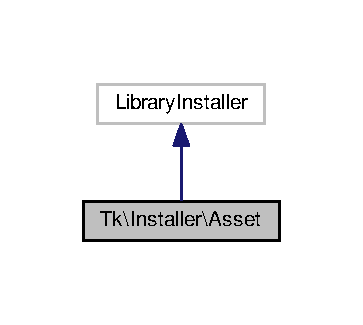
\includegraphics[width=174pt]{classTk_1_1Installer_1_1Asset__inherit__graph}
\end{center}
\end{figure}
\subsection*{Public Member Functions}
\begin{DoxyCompactItemize}
\item 
\hyperlink{classTk_1_1Installer_1_1Asset_a132a52a1330c45cf999b0d161ea4936a}{get\+Package\+Base\+Path} (Package\+Interface \$package)
\item 
\hyperlink{classTk_1_1Installer_1_1Asset_af3a8834946b96b149859e916b06569c4}{supports} (\$package\+Type)
\end{DoxyCompactItemize}


\subsection{Member Function Documentation}
\hypertarget{classTk_1_1Installer_1_1Asset_a132a52a1330c45cf999b0d161ea4936a}{\index{Tk\+::\+Installer\+::\+Asset@{Tk\+::\+Installer\+::\+Asset}!get\+Package\+Base\+Path@{get\+Package\+Base\+Path}}
\index{get\+Package\+Base\+Path@{get\+Package\+Base\+Path}!Tk\+::\+Installer\+::\+Asset@{Tk\+::\+Installer\+::\+Asset}}
\subsubsection[{get\+Package\+Base\+Path}]{\setlength{\rightskip}{0pt plus 5cm}Tk\textbackslash{}\+Installer\textbackslash{}\+Asset\+::get\+Package\+Base\+Path (
\begin{DoxyParamCaption}
\item[{Package\+Interface}]{\$package}
\end{DoxyParamCaption}
)}}\label{classTk_1_1Installer_1_1Asset_a132a52a1330c45cf999b0d161ea4936a}
\hypertarget{classTk_1_1Installer_1_1Asset_af3a8834946b96b149859e916b06569c4}{\index{Tk\+::\+Installer\+::\+Asset@{Tk\+::\+Installer\+::\+Asset}!supports@{supports}}
\index{supports@{supports}!Tk\+::\+Installer\+::\+Asset@{Tk\+::\+Installer\+::\+Asset}}
\subsubsection[{supports}]{\setlength{\rightskip}{0pt plus 5cm}Tk\textbackslash{}\+Installer\textbackslash{}\+Asset\+::supports (
\begin{DoxyParamCaption}
\item[{}]{\$package\+Type}
\end{DoxyParamCaption}
)}}\label{classTk_1_1Installer_1_1Asset_af3a8834946b96b149859e916b06569c4}


The documentation for this class was generated from the following file\+:\begin{DoxyCompactItemize}
\item 
vendor/ttek/tk-\/installers/\+Tk/\+Installer/Asset.\+php\end{DoxyCompactItemize}

\hypertarget{classTk_1_1Installer_1_1AssetPlugin}{\section{Tk\textbackslash{}Installer\textbackslash{}Asset\+Plugin Class Reference}
\label{classTk_1_1Installer_1_1AssetPlugin}\index{Tk\textbackslash{}\+Installer\textbackslash{}\+Asset\+Plugin@{Tk\textbackslash{}\+Installer\textbackslash{}\+Asset\+Plugin}}
}


Inheritance diagram for Tk\textbackslash{}Installer\textbackslash{}Asset\+Plugin\+:\nopagebreak
\begin{figure}[H]
\begin{center}
\leavevmode
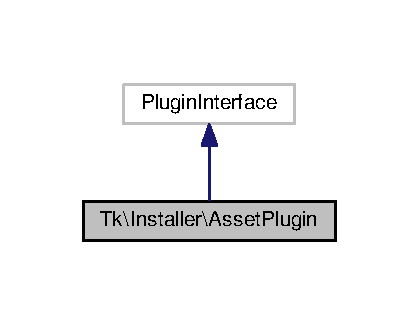
\includegraphics[width=201pt]{classTk_1_1Installer_1_1AssetPlugin__inherit__graph}
\end{center}
\end{figure}
\subsection*{Public Member Functions}
\begin{DoxyCompactItemize}
\item 
\hypertarget{classTk_1_1Installer_1_1AssetPlugin_a81d4cccef9792f534f1669276617c303}{{\bfseries activate} (Composer \$composer, I\+O\+Interface \$io)}\label{classTk_1_1Installer_1_1AssetPlugin_a81d4cccef9792f534f1669276617c303}

\end{DoxyCompactItemize}


The documentation for this class was generated from the following file\+:\begin{DoxyCompactItemize}
\item 
vendor/ttek/tk-\/installers/\+Tk/\+Installer/Asset\+Plugin.\+php\end{DoxyCompactItemize}

\hypertarget{classDom_1_1Renderer_1_1AutoRenderer}{\section{Dom\textbackslash{}Renderer\textbackslash{}Auto\+Renderer Class Reference}
\label{classDom_1_1Renderer_1_1AutoRenderer}\index{Dom\textbackslash{}\+Renderer\textbackslash{}\+Auto\+Renderer@{Dom\textbackslash{}\+Renderer\textbackslash{}\+Auto\+Renderer}}
}


Inheritance diagram for Dom\textbackslash{}Renderer\textbackslash{}Auto\+Renderer\+:\nopagebreak
\begin{figure}[H]
\begin{center}
\leavevmode
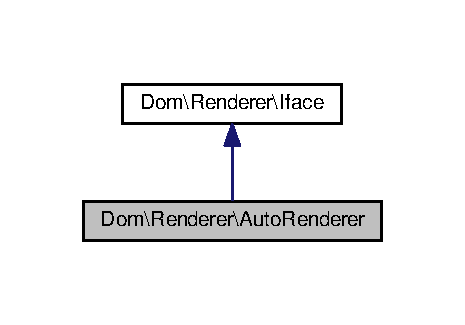
\includegraphics[width=223pt]{classDom_1_1Renderer_1_1AutoRenderer__inherit__graph}
\end{center}
\end{figure}
\subsection*{Public Member Functions}
\begin{DoxyCompactItemize}
\item 
\hyperlink{classDom_1_1Renderer_1_1AutoRenderer_a87d7af23e35fcbe2f3d5b31c8c5f0504}{\+\_\+\+\_\+construct} (\$template=null, \$data=null)
\item 
\hyperlink{classDom_1_1Renderer_1_1AutoRenderer_ac73a67b447e94321d31bd4f388f1b90a}{exists} (\$name)
\item 
\hyperlink{classDom_1_1Renderer_1_1AutoRenderer_ada481677e5252d2aa5cd03b46b6637f5}{set} (\$name, \$val)
\item 
\hyperlink{classDom_1_1Renderer_1_1AutoRenderer_ac9a2979a26a01180f2723d9dcbd97a1f}{get} (\$name=null)
\item 
\hyperlink{classDom_1_1Renderer_1_1AutoRenderer_a71ad96ed156aa79d45058b3bf372e73d}{show} ()
\item 
\hyperlink{classDom_1_1Renderer_1_1AutoRenderer_a8c34c043c962f53241f825579839750c}{set\+Template} (\$template)
\item 
\hyperlink{classDom_1_1Renderer_1_1AutoRenderer_a7c6ac2e26298cf2a8be324f6e44056cf}{get\+Template} ()
\item 
\hyperlink{classDom_1_1Renderer_1_1AutoRenderer_a0172677627adb5372fb026d177d57951}{has\+Template} ()
\item 
\hyperlink{classDom_1_1Renderer_1_1AutoRenderer_aa2b0c92e699c2e5454ed6da1de19c0bd}{to\+String} (\$params=null)
\item 
\hyperlink{classDom_1_1Renderer_1_1AutoRenderer_a79b361f403c09d7d1ccc81933b718017}{\+\_\+\+\_\+to\+String} ()
\end{DoxyCompactItemize}
\subsection*{Protected Member Functions}
\begin{DoxyCompactItemize}
\item 
\hyperlink{classDom_1_1Renderer_1_1AutoRenderer_a3b70adccf8b6bfe1f1cea70f9f5b61c1}{show\+Repeat} (\$template, \$var\+Val=null)
\item 
\hyperlink{classDom_1_1Renderer_1_1AutoRenderer_a2a0ec28ecc71a00879f8eb5b01f2d757}{show\+Choice} (\$template, \$var\+Val=null)
\item 
\hyperlink{classDom_1_1Renderer_1_1AutoRenderer_a22152a42a4755f4cea0cdc35ca7da5ca}{show\+Vars} (\$template, \$var\+Val=null)
\item 
\hyperlink{classDom_1_1Renderer_1_1AutoRenderer_af00edcb9f6d79f99f3b29fb4e4f47f05}{get\+Parameter} (\$raw\+Param, \$var\+Val=null)
\item 
\hyperlink{classDom_1_1Renderer_1_1AutoRenderer_a33948b5b6b5168f0b33c9f3c59f9ad70}{access\+Array} (\$array, \$keys)
\item 
\hyperlink{classDom_1_1Renderer_1_1AutoRenderer_ac9a3ade75e9579add0a93c613ab4b822}{var\+To\+Str} (\$val, \$i=0)
\end{DoxyCompactItemize}
\subsection*{Protected Attributes}
\begin{DoxyCompactItemize}
\item 
\hypertarget{classDom_1_1Renderer_1_1AutoRenderer_a73b9fa3881a3433725dde8340265c2ff}{{\bfseries \$template} = null}\label{classDom_1_1Renderer_1_1AutoRenderer_a73b9fa3881a3433725dde8340265c2ff}

\end{DoxyCompactItemize}


\subsection{Detailed Description}
For classes that render dom templates.

This is a good base for all renderer objects that implement the  it can guide you to create templates that can be inserted into other template objects.

If the current template is null then the magic method \+\_\+\+\_\+make\+Template() will be called to create an internal template. This is a good way to create a default template. But be aware that this will be a new template and will have to be inserted into its parent using the \+::insert\+Template() method.

\+: This object is currently under development and may change.. \begin{DoxyAuthor}{Author}
Michael Mifsud \href{mailto:info@tropotek.com}{\tt info@tropotek.\+com} \hyperlink{}{Copyright 2007 Michael Mifsud }
\end{DoxyAuthor}


\subsection{Constructor \& Destructor Documentation}
\hypertarget{classDom_1_1Renderer_1_1AutoRenderer_a87d7af23e35fcbe2f3d5b31c8c5f0504}{\index{Dom\+::\+Renderer\+::\+Auto\+Renderer@{Dom\+::\+Renderer\+::\+Auto\+Renderer}!\+\_\+\+\_\+construct@{\+\_\+\+\_\+construct}}
\index{\+\_\+\+\_\+construct@{\+\_\+\+\_\+construct}!Dom\+::\+Renderer\+::\+Auto\+Renderer@{Dom\+::\+Renderer\+::\+Auto\+Renderer}}
\subsubsection[{\+\_\+\+\_\+construct}]{\setlength{\rightskip}{0pt plus 5cm}Dom\textbackslash{}\+Renderer\textbackslash{}\+Auto\+Renderer\+::\+\_\+\+\_\+construct (
\begin{DoxyParamCaption}
\item[{}]{\$template = {\ttfamily null}, }
\item[{}]{\$data = {\ttfamily null}}
\end{DoxyParamCaption}
)}}\label{classDom_1_1Renderer_1_1AutoRenderer_a87d7af23e35fcbe2f3d5b31c8c5f0504}
Constructor


\begin{DoxyParams}[1]{Parameters}
array & {\em \$data} & \\
\hline
\hyperlink{classDom_1_1Template}{Template} & {\em \$template} & \\
\hline
\end{DoxyParams}


\subsection{Member Function Documentation}
\hypertarget{classDom_1_1Renderer_1_1AutoRenderer_a79b361f403c09d7d1ccc81933b718017}{\index{Dom\+::\+Renderer\+::\+Auto\+Renderer@{Dom\+::\+Renderer\+::\+Auto\+Renderer}!\+\_\+\+\_\+to\+String@{\+\_\+\+\_\+to\+String}}
\index{\+\_\+\+\_\+to\+String@{\+\_\+\+\_\+to\+String}!Dom\+::\+Renderer\+::\+Auto\+Renderer@{Dom\+::\+Renderer\+::\+Auto\+Renderer}}
\subsubsection[{\+\_\+\+\_\+to\+String}]{\setlength{\rightskip}{0pt plus 5cm}Dom\textbackslash{}\+Renderer\textbackslash{}\+Auto\+Renderer\+::\+\_\+\+\_\+to\+String (
\begin{DoxyParamCaption}
{}
\end{DoxyParamCaption}
)}}\label{classDom_1_1Renderer_1_1AutoRenderer_a79b361f403c09d7d1ccc81933b718017}
\+\_\+\+\_\+to\+String

\begin{DoxyReturn}{Returns}
string 
\end{DoxyReturn}
\hypertarget{classDom_1_1Renderer_1_1AutoRenderer_a33948b5b6b5168f0b33c9f3c59f9ad70}{\index{Dom\+::\+Renderer\+::\+Auto\+Renderer@{Dom\+::\+Renderer\+::\+Auto\+Renderer}!access\+Array@{access\+Array}}
\index{access\+Array@{access\+Array}!Dom\+::\+Renderer\+::\+Auto\+Renderer@{Dom\+::\+Renderer\+::\+Auto\+Renderer}}
\subsubsection[{access\+Array}]{\setlength{\rightskip}{0pt plus 5cm}Dom\textbackslash{}\+Renderer\textbackslash{}\+Auto\+Renderer\+::access\+Array (
\begin{DoxyParamCaption}
\item[{}]{\$array, }
\item[{}]{\$keys}
\end{DoxyParamCaption}
)\hspace{0.3cm}{\ttfamily [protected]}}}\label{classDom_1_1Renderer_1_1AutoRenderer_a33948b5b6b5168f0b33c9f3c59f9ad70}
access\+Array


\begin{DoxyParams}[1]{Parameters}
array & {\em \$array} & \\
\hline
string & {\em \$keys} & Example \char`\"{}\mbox{[}'test'\mbox{]}\mbox{[}0\mbox{]}\mbox{[}'item'\mbox{]}\char`\"{} \\
\hline
\end{DoxyParams}
\begin{DoxyReturn}{Returns}
mixed 
\end{DoxyReturn}

\begin{DoxyExceptions}{Exceptions}
{\em } & Invalid\+Argument\+Exception \\
\hline
\end{DoxyExceptions}
\hypertarget{classDom_1_1Renderer_1_1AutoRenderer_ac73a67b447e94321d31bd4f388f1b90a}{\index{Dom\+::\+Renderer\+::\+Auto\+Renderer@{Dom\+::\+Renderer\+::\+Auto\+Renderer}!exists@{exists}}
\index{exists@{exists}!Dom\+::\+Renderer\+::\+Auto\+Renderer@{Dom\+::\+Renderer\+::\+Auto\+Renderer}}
\subsubsection[{exists}]{\setlength{\rightskip}{0pt plus 5cm}Dom\textbackslash{}\+Renderer\textbackslash{}\+Auto\+Renderer\+::exists (
\begin{DoxyParamCaption}
\item[{}]{\$name}
\end{DoxyParamCaption}
)}}\label{classDom_1_1Renderer_1_1AutoRenderer_ac73a67b447e94321d31bd4f388f1b90a}
Test if an array key exists in the renderer data list


\begin{DoxyParams}{Parameters}
{\em \$name} & \\
\hline
\end{DoxyParams}
\begin{DoxyReturn}{Returns}
bool 
\end{DoxyReturn}
\hypertarget{classDom_1_1Renderer_1_1AutoRenderer_ac9a2979a26a01180f2723d9dcbd97a1f}{\index{Dom\+::\+Renderer\+::\+Auto\+Renderer@{Dom\+::\+Renderer\+::\+Auto\+Renderer}!get@{get}}
\index{get@{get}!Dom\+::\+Renderer\+::\+Auto\+Renderer@{Dom\+::\+Renderer\+::\+Auto\+Renderer}}
\subsubsection[{get}]{\setlength{\rightskip}{0pt plus 5cm}Dom\textbackslash{}\+Renderer\textbackslash{}\+Auto\+Renderer\+::get (
\begin{DoxyParamCaption}
\item[{}]{\$name = {\ttfamily null}}
\end{DoxyParamCaption}
)}}\label{classDom_1_1Renderer_1_1AutoRenderer_ac9a2979a26a01180f2723d9dcbd97a1f}
Get an element from the renderer data list


\begin{DoxyParams}[1]{Parameters}
string & {\em \$name} & If not set then all the data array is returned \\
\hline
\end{DoxyParams}
\begin{DoxyReturn}{Returns}
mixed 
\end{DoxyReturn}
\hypertarget{classDom_1_1Renderer_1_1AutoRenderer_af00edcb9f6d79f99f3b29fb4e4f47f05}{\index{Dom\+::\+Renderer\+::\+Auto\+Renderer@{Dom\+::\+Renderer\+::\+Auto\+Renderer}!get\+Parameter@{get\+Parameter}}
\index{get\+Parameter@{get\+Parameter}!Dom\+::\+Renderer\+::\+Auto\+Renderer@{Dom\+::\+Renderer\+::\+Auto\+Renderer}}
\subsubsection[{get\+Parameter}]{\setlength{\rightskip}{0pt plus 5cm}Dom\textbackslash{}\+Renderer\textbackslash{}\+Auto\+Renderer\+::get\+Parameter (
\begin{DoxyParamCaption}
\item[{}]{\$raw\+Param, }
\item[{}]{\$var\+Val = {\ttfamily null}}
\end{DoxyParamCaption}
)\hspace{0.3cm}{\ttfamily [protected]}}}\label{classDom_1_1Renderer_1_1AutoRenderer_af00edcb9f6d79f99f3b29fb4e4f47f05}
get\+Parameter


\begin{DoxyParams}[1]{Parameters}
string & {\em \$raw\+Param} & \\
\hline
string | null & {\em \$var\+Val} & \\
\hline
\end{DoxyParams}
\begin{DoxyReturn}{Returns}
mixed 
\end{DoxyReturn}
\hypertarget{classDom_1_1Renderer_1_1AutoRenderer_a7c6ac2e26298cf2a8be324f6e44056cf}{\index{Dom\+::\+Renderer\+::\+Auto\+Renderer@{Dom\+::\+Renderer\+::\+Auto\+Renderer}!get\+Template@{get\+Template}}
\index{get\+Template@{get\+Template}!Dom\+::\+Renderer\+::\+Auto\+Renderer@{Dom\+::\+Renderer\+::\+Auto\+Renderer}}
\subsubsection[{get\+Template}]{\setlength{\rightskip}{0pt plus 5cm}Dom\textbackslash{}\+Renderer\textbackslash{}\+Auto\+Renderer\+::get\+Template (
\begin{DoxyParamCaption}
{}
\end{DoxyParamCaption}
)}}\label{classDom_1_1Renderer_1_1AutoRenderer_a7c6ac2e26298cf2a8be324f6e44056cf}
Get the template This method will try to call the magic method \+\_\+\+\_\+make\+Template to get a template if none exits. Use this for objects that use internal templates.

\begin{DoxyReturn}{Returns}
\hyperlink{classDom_1_1Template}{Template} 
\end{DoxyReturn}


Implements \hyperlink{interfaceDom_1_1Renderer_1_1Iface_ad24995320dbbbd8a1796c1d13518012c}{Dom\textbackslash{}\+Renderer\textbackslash{}\+Iface}.

\hypertarget{classDom_1_1Renderer_1_1AutoRenderer_a0172677627adb5372fb026d177d57951}{\index{Dom\+::\+Renderer\+::\+Auto\+Renderer@{Dom\+::\+Renderer\+::\+Auto\+Renderer}!has\+Template@{has\+Template}}
\index{has\+Template@{has\+Template}!Dom\+::\+Renderer\+::\+Auto\+Renderer@{Dom\+::\+Renderer\+::\+Auto\+Renderer}}
\subsubsection[{has\+Template}]{\setlength{\rightskip}{0pt plus 5cm}Dom\textbackslash{}\+Renderer\textbackslash{}\+Auto\+Renderer\+::has\+Template (
\begin{DoxyParamCaption}
{}
\end{DoxyParamCaption}
)}}\label{classDom_1_1Renderer_1_1AutoRenderer_a0172677627adb5372fb026d177d57951}
Test if this renderer has a template and is not N\+U\+L\+L

\begin{DoxyReturn}{Returns}
bool 
\end{DoxyReturn}
\hypertarget{classDom_1_1Renderer_1_1AutoRenderer_ada481677e5252d2aa5cd03b46b6637f5}{\index{Dom\+::\+Renderer\+::\+Auto\+Renderer@{Dom\+::\+Renderer\+::\+Auto\+Renderer}!set@{set}}
\index{set@{set}!Dom\+::\+Renderer\+::\+Auto\+Renderer@{Dom\+::\+Renderer\+::\+Auto\+Renderer}}
\subsubsection[{set}]{\setlength{\rightskip}{0pt plus 5cm}Dom\textbackslash{}\+Renderer\textbackslash{}\+Auto\+Renderer\+::set (
\begin{DoxyParamCaption}
\item[{}]{\$name, }
\item[{}]{\$val}
\end{DoxyParamCaption}
)}}\label{classDom_1_1Renderer_1_1AutoRenderer_ada481677e5252d2aa5cd03b46b6637f5}
Add an item to the renderer data list


\begin{DoxyParams}[1]{Parameters}
string & {\em \$name} & \\
\hline
mixed & {\em \$val} & \\
\hline
\end{DoxyParams}
\hypertarget{classDom_1_1Renderer_1_1AutoRenderer_a8c34c043c962f53241f825579839750c}{\index{Dom\+::\+Renderer\+::\+Auto\+Renderer@{Dom\+::\+Renderer\+::\+Auto\+Renderer}!set\+Template@{set\+Template}}
\index{set\+Template@{set\+Template}!Dom\+::\+Renderer\+::\+Auto\+Renderer@{Dom\+::\+Renderer\+::\+Auto\+Renderer}}
\subsubsection[{set\+Template}]{\setlength{\rightskip}{0pt plus 5cm}Dom\textbackslash{}\+Renderer\textbackslash{}\+Auto\+Renderer\+::set\+Template (
\begin{DoxyParamCaption}
\item[{}]{\$template}
\end{DoxyParamCaption}
)}}\label{classDom_1_1Renderer_1_1AutoRenderer_a8c34c043c962f53241f825579839750c}
Set a new template for this renderer.


\begin{DoxyParams}[1]{Parameters}
\hyperlink{classDom_1_1Template}{Template} & {\em \$template} & \\
\hline
\end{DoxyParams}
\begin{DoxyReturn}{Returns}
\$this 
\end{DoxyReturn}


Implements \hyperlink{interfaceDom_1_1Renderer_1_1Iface_a6e4c7ff3f90a9b1a26bc08bf6e1408d6}{Dom\textbackslash{}\+Renderer\textbackslash{}\+Iface}.

\hypertarget{classDom_1_1Renderer_1_1AutoRenderer_a71ad96ed156aa79d45058b3bf372e73d}{\index{Dom\+::\+Renderer\+::\+Auto\+Renderer@{Dom\+::\+Renderer\+::\+Auto\+Renderer}!show@{show}}
\index{show@{show}!Dom\+::\+Renderer\+::\+Auto\+Renderer@{Dom\+::\+Renderer\+::\+Auto\+Renderer}}
\subsubsection[{show}]{\setlength{\rightskip}{0pt plus 5cm}Dom\textbackslash{}\+Renderer\textbackslash{}\+Auto\+Renderer\+::show (
\begin{DoxyParamCaption}
{}
\end{DoxyParamCaption}
)}}\label{classDom_1_1Renderer_1_1AutoRenderer_a71ad96ed156aa79d45058b3bf372e73d}
Execute the renderer. This method can optionally return a \hyperlink{classDom_1_1Template}{Template} Object or H\+T\+M\+L/\+X\+M\+L string depending on your framework requirements

\begin{DoxyReturn}{Returns}
\hyperlink{classDom_1_1Template}{Template} $\vert$ string 
\end{DoxyReturn}


Implements \hyperlink{interfaceDom_1_1Renderer_1_1Iface_a79a0ba41fb6714d69156891d6326bd33}{Dom\textbackslash{}\+Renderer\textbackslash{}\+Iface}.

\hypertarget{classDom_1_1Renderer_1_1AutoRenderer_a2a0ec28ecc71a00879f8eb5b01f2d757}{\index{Dom\+::\+Renderer\+::\+Auto\+Renderer@{Dom\+::\+Renderer\+::\+Auto\+Renderer}!show\+Choice@{show\+Choice}}
\index{show\+Choice@{show\+Choice}!Dom\+::\+Renderer\+::\+Auto\+Renderer@{Dom\+::\+Renderer\+::\+Auto\+Renderer}}
\subsubsection[{show\+Choice}]{\setlength{\rightskip}{0pt plus 5cm}Dom\textbackslash{}\+Renderer\textbackslash{}\+Auto\+Renderer\+::show\+Choice (
\begin{DoxyParamCaption}
\item[{}]{\$template, }
\item[{}]{\$var\+Val = {\ttfamily null}}
\end{DoxyParamCaption}
)\hspace{0.3cm}{\ttfamily [protected]}}}\label{classDom_1_1Renderer_1_1AutoRenderer_a2a0ec28ecc71a00879f8eb5b01f2d757}
Render all vars found in the template


\begin{DoxyParams}[1]{Parameters}
\hyperlink{classDom_1_1Template}{Template} & {\em \$template} & \\
\hline
string | null & {\em \$var\+Val} & \\
\hline
\end{DoxyParams}
\begin{DoxyReturn}{Returns}
\$this 
\end{DoxyReturn}
\hypertarget{classDom_1_1Renderer_1_1AutoRenderer_a3b70adccf8b6bfe1f1cea70f9f5b61c1}{\index{Dom\+::\+Renderer\+::\+Auto\+Renderer@{Dom\+::\+Renderer\+::\+Auto\+Renderer}!show\+Repeat@{show\+Repeat}}
\index{show\+Repeat@{show\+Repeat}!Dom\+::\+Renderer\+::\+Auto\+Renderer@{Dom\+::\+Renderer\+::\+Auto\+Renderer}}
\subsubsection[{show\+Repeat}]{\setlength{\rightskip}{0pt plus 5cm}Dom\textbackslash{}\+Renderer\textbackslash{}\+Auto\+Renderer\+::show\+Repeat (
\begin{DoxyParamCaption}
\item[{}]{\$template, }
\item[{}]{\$var\+Val = {\ttfamily null}}
\end{DoxyParamCaption}
)\hspace{0.3cm}{\ttfamily [protected]}}}\label{classDom_1_1Renderer_1_1AutoRenderer_a3b70adccf8b6bfe1f1cea70f9f5b61c1}
Render all vars found in the template


\begin{DoxyParams}[1]{Parameters}
\hyperlink{classDom_1_1Template}{Template} & {\em \$template} & \\
\hline
string | null & {\em \$var\+Val} & \\
\hline
\end{DoxyParams}
\begin{DoxyReturn}{Returns}
\$this 
\end{DoxyReturn}
\hypertarget{classDom_1_1Renderer_1_1AutoRenderer_a22152a42a4755f4cea0cdc35ca7da5ca}{\index{Dom\+::\+Renderer\+::\+Auto\+Renderer@{Dom\+::\+Renderer\+::\+Auto\+Renderer}!show\+Vars@{show\+Vars}}
\index{show\+Vars@{show\+Vars}!Dom\+::\+Renderer\+::\+Auto\+Renderer@{Dom\+::\+Renderer\+::\+Auto\+Renderer}}
\subsubsection[{show\+Vars}]{\setlength{\rightskip}{0pt plus 5cm}Dom\textbackslash{}\+Renderer\textbackslash{}\+Auto\+Renderer\+::show\+Vars (
\begin{DoxyParamCaption}
\item[{}]{\$template, }
\item[{}]{\$var\+Val = {\ttfamily null}}
\end{DoxyParamCaption}
)\hspace{0.3cm}{\ttfamily [protected]}}}\label{classDom_1_1Renderer_1_1AutoRenderer_a22152a42a4755f4cea0cdc35ca7da5ca}
Render all vars found in the template


\begin{DoxyParams}[1]{Parameters}
\hyperlink{classDom_1_1Template}{Template} & {\em \$template} & \\
\hline
string | null & {\em \$var\+Val} & \\
\hline
\end{DoxyParams}
\begin{DoxyReturn}{Returns}
\$this 
\end{DoxyReturn}

\begin{DoxyExceptions}{Exceptions}
{\em \hyperlink{classDom_1_1Exception}{Exception}} & \\
\hline
\end{DoxyExceptions}
\hypertarget{classDom_1_1Renderer_1_1AutoRenderer_aa2b0c92e699c2e5454ed6da1de19c0bd}{\index{Dom\+::\+Renderer\+::\+Auto\+Renderer@{Dom\+::\+Renderer\+::\+Auto\+Renderer}!to\+String@{to\+String}}
\index{to\+String@{to\+String}!Dom\+::\+Renderer\+::\+Auto\+Renderer@{Dom\+::\+Renderer\+::\+Auto\+Renderer}}
\subsubsection[{to\+String}]{\setlength{\rightskip}{0pt plus 5cm}Dom\textbackslash{}\+Renderer\textbackslash{}\+Auto\+Renderer\+::to\+String (
\begin{DoxyParamCaption}
\item[{}]{\$params = {\ttfamily null}}
\end{DoxyParamCaption}
)}}\label{classDom_1_1Renderer_1_1AutoRenderer_aa2b0c92e699c2e5454ed6da1de19c0bd}
Parse the template with the supplied params


\begin{DoxyParams}[1]{Parameters}
array & {\em \$params} & \\
\hline
\end{DoxyParams}
\begin{DoxyReturn}{Returns}
string 
\end{DoxyReturn}
\hypertarget{classDom_1_1Renderer_1_1AutoRenderer_ac9a3ade75e9579add0a93c613ab4b822}{\index{Dom\+::\+Renderer\+::\+Auto\+Renderer@{Dom\+::\+Renderer\+::\+Auto\+Renderer}!var\+To\+Str@{var\+To\+Str}}
\index{var\+To\+Str@{var\+To\+Str}!Dom\+::\+Renderer\+::\+Auto\+Renderer@{Dom\+::\+Renderer\+::\+Auto\+Renderer}}
\subsubsection[{var\+To\+Str}]{\setlength{\rightskip}{0pt plus 5cm}Dom\textbackslash{}\+Renderer\textbackslash{}\+Auto\+Renderer\+::var\+To\+Str (
\begin{DoxyParamCaption}
\item[{}]{\$val, }
\item[{}]{\$i = {\ttfamily 0}}
\end{DoxyParamCaption}
)\hspace{0.3cm}{\ttfamily [protected]}}}\label{classDom_1_1Renderer_1_1AutoRenderer_ac9a3ade75e9579add0a93c613ab4b822}
Get the string from an object/array/string...


\begin{DoxyParams}[1]{Parameters}
mixed & {\em \$val} & \\
\hline
int & {\em \$i} & Used to get the index from an array Default 0 the first item \\
\hline
\end{DoxyParams}
\begin{DoxyReturn}{Returns}
string 
\end{DoxyReturn}


The documentation for this class was generated from the following file\+:\begin{DoxyCompactItemize}
\item 
vendor/ttek/tk-\/domtemplate/\+Dom/\+Renderer/Auto\+Renderer.\+php\end{DoxyCompactItemize}

\hypertarget{classTk_1_1Db_1_1Backup}{\section{Tk\textbackslash{}Db\textbackslash{}Backup Class Reference}
\label{classTk_1_1Db_1_1Backup}\index{Tk\textbackslash{}\+Db\textbackslash{}\+Backup@{Tk\textbackslash{}\+Db\textbackslash{}\+Backup}}
}
\subsection*{Public Member Functions}
\begin{DoxyCompactItemize}
\item 
\hyperlink{classTk_1_1Db_1_1Backup_aa753fa8efaa408463a33c6322fa6bb5c}{\+\_\+\+\_\+construct} (\hyperlink{classTk_1_1Db_1_1Pdo}{Pdo} \$db)
\item 
\hyperlink{classTk_1_1Db_1_1Backup_a9c770ba9f7e9a177974edb35cdc47a5f}{export} (\$out\+File, \$drop\+Table=true)
\item 
\hyperlink{classTk_1_1Db_1_1Backup_ad1af7d1b4ed883769e127481b469d08b}{import} (\$in\+File)
\end{DoxyCompactItemize}


\subsection{Detailed Description}
Class \hyperlink{classTk_1_1Db_1_1Backup}{Backup}

\hyperlink{classTk_1_1Db_1_1Backup}{Backup} and restore function for a full My\+S\+Q\+L database

\begin{DoxyAuthor}{Author}
Tropotek \href{mailto:info@tropotek.com}{\tt info@tropotek.\+com} \hyperlink{}{Copyright 2015 Tropotek }
\end{DoxyAuthor}


\subsection{Constructor \& Destructor Documentation}
\hypertarget{classTk_1_1Db_1_1Backup_aa753fa8efaa408463a33c6322fa6bb5c}{\index{Tk\+::\+Db\+::\+Backup@{Tk\+::\+Db\+::\+Backup}!\+\_\+\+\_\+construct@{\+\_\+\+\_\+construct}}
\index{\+\_\+\+\_\+construct@{\+\_\+\+\_\+construct}!Tk\+::\+Db\+::\+Backup@{Tk\+::\+Db\+::\+Backup}}
\subsubsection[{\+\_\+\+\_\+construct}]{\setlength{\rightskip}{0pt plus 5cm}Tk\textbackslash{}\+Db\textbackslash{}\+Backup\+::\+\_\+\+\_\+construct (
\begin{DoxyParamCaption}
\item[{{\bf Pdo}}]{\$db}
\end{DoxyParamCaption}
)}}\label{classTk_1_1Db_1_1Backup_aa753fa8efaa408463a33c6322fa6bb5c}
construct


\begin{DoxyParams}[1]{Parameters}
\hyperlink{classTk_1_1Db_1_1Pdo}{Pdo} & {\em \$db} & \\
\hline
\end{DoxyParams}


\subsection{Member Function Documentation}
\hypertarget{classTk_1_1Db_1_1Backup_a9c770ba9f7e9a177974edb35cdc47a5f}{\index{Tk\+::\+Db\+::\+Backup@{Tk\+::\+Db\+::\+Backup}!export@{export}}
\index{export@{export}!Tk\+::\+Db\+::\+Backup@{Tk\+::\+Db\+::\+Backup}}
\subsubsection[{export}]{\setlength{\rightskip}{0pt plus 5cm}Tk\textbackslash{}\+Db\textbackslash{}\+Backup\+::export (
\begin{DoxyParamCaption}
\item[{}]{\$out\+File, }
\item[{}]{\$drop\+Table = {\ttfamily true}}
\end{DoxyParamCaption}
)}}\label{classTk_1_1Db_1_1Backup_a9c770ba9f7e9a177974edb35cdc47a5f}
Create a backup file of the database The full filename and path will be returned.


\begin{DoxyParams}[1]{Parameters}
string & {\em \$out\+File} & \\
\hline
bool & {\em \$drop\+Table} & \\
\hline
\end{DoxyParams}
\begin{DoxyReturn}{Returns}
string 
\end{DoxyReturn}

\begin{DoxyExceptions}{Exceptions}
{\em \hyperlink{classTk_1_1Db_1_1Exception}{Exception}} & \\
\hline
\end{DoxyExceptions}
\hypertarget{classTk_1_1Db_1_1Backup_ad1af7d1b4ed883769e127481b469d08b}{\index{Tk\+::\+Db\+::\+Backup@{Tk\+::\+Db\+::\+Backup}!import@{import}}
\index{import@{import}!Tk\+::\+Db\+::\+Backup@{Tk\+::\+Db\+::\+Backup}}
\subsubsection[{import}]{\setlength{\rightskip}{0pt plus 5cm}Tk\textbackslash{}\+Db\textbackslash{}\+Backup\+::import (
\begin{DoxyParamCaption}
\item[{}]{\$in\+File}
\end{DoxyParamCaption}
)}}\label{classTk_1_1Db_1_1Backup_ad1af7d1b4ed883769e127481b469d08b}
Restore a database backup file from a file


\begin{DoxyParams}[1]{Parameters}
string & {\em \$in\+File} & \\
\hline
\end{DoxyParams}
\begin{DoxyReturn}{Returns}
bool 
\end{DoxyReturn}

\begin{DoxyExceptions}{Exceptions}
{\em \hyperlink{classTk_1_1Db_1_1Exception}{Exception}} & \\
\hline
\end{DoxyExceptions}


The documentation for this class was generated from the following file\+:\begin{DoxyCompactItemize}
\item 
vendor/ttek/tk-\/framework/\+Tk/\+Db/\+Utils/Backup.\+php\end{DoxyCompactItemize}

\hypertarget{classTk_1_1Table_1_1Cell_1_1Boolean}{\section{Tk\textbackslash{}Table\textbackslash{}Cell\textbackslash{}Boolean Class Reference}
\label{classTk_1_1Table_1_1Cell_1_1Boolean}\index{Tk\textbackslash{}\+Table\textbackslash{}\+Cell\textbackslash{}\+Boolean@{Tk\textbackslash{}\+Table\textbackslash{}\+Cell\textbackslash{}\+Boolean}}
}


Inheritance diagram for Tk\textbackslash{}Table\textbackslash{}Cell\textbackslash{}Boolean\+:\nopagebreak
\begin{figure}[H]
\begin{center}
\leavevmode
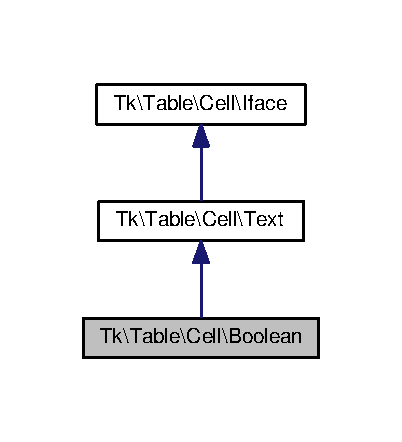
\includegraphics[width=193pt]{classTk_1_1Table_1_1Cell_1_1Boolean__inherit__graph}
\end{center}
\end{figure}
\subsection*{Public Member Functions}
\begin{DoxyCompactItemize}
\item 
\hypertarget{classTk_1_1Table_1_1Cell_1_1Boolean_a05048e18d4f23c81284208bf3342cc5b}{{\bfseries get\+Property\+Value} (\$obj, \$property)}\label{classTk_1_1Table_1_1Cell_1_1Boolean_a05048e18d4f23c81284208bf3342cc5b}

\end{DoxyCompactItemize}
\subsection*{Additional Inherited Members}


\subsection{Detailed Description}
Class \hyperlink{classTk_1_1Table_1_1Cell_1_1Text}{Text}

\begin{DoxyAuthor}{Author}
Michael Mifsud \href{mailto:info@tropotek.com}{\tt info@tropotek.\+com} \hyperlink{}{Copyright 2015 Michael Mifsud }
\end{DoxyAuthor}


The documentation for this class was generated from the following file\+:\begin{DoxyCompactItemize}
\item 
vendor/ttek/tk-\/table/\+Tk/\+Table/\+Cell/Boolean.\+php\end{DoxyCompactItemize}

\hypertarget{classTk_1_1Form_1_1Type_1_1Boolean}{\section{Tk\textbackslash{}Form\textbackslash{}Type\textbackslash{}Boolean Class Reference}
\label{classTk_1_1Form_1_1Type_1_1Boolean}\index{Tk\textbackslash{}\+Form\textbackslash{}\+Type\textbackslash{}\+Boolean@{Tk\textbackslash{}\+Form\textbackslash{}\+Type\textbackslash{}\+Boolean}}
}


Inheritance diagram for Tk\textbackslash{}Form\textbackslash{}Type\textbackslash{}Boolean\+:\nopagebreak
\begin{figure}[H]
\begin{center}
\leavevmode
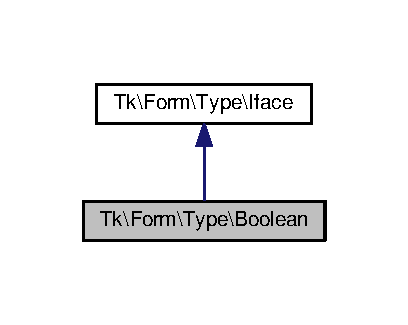
\includegraphics[width=196pt]{classTk_1_1Form_1_1Type_1_1Boolean__inherit__graph}
\end{center}
\end{figure}
\subsection*{Public Member Functions}
\begin{DoxyCompactItemize}
\item 
\hyperlink{classTk_1_1Form_1_1Type_1_1Boolean_a96ea72276998c8698afe1e14b2a5481d}{to\+Type} (\$array)
\item 
\hyperlink{classTk_1_1Form_1_1Type_1_1Boolean_a9e9176a54fcce8ba225024f737caf8f5}{to\+Text} (\$array)
\item 
\hyperlink{classTk_1_1Form_1_1Type_1_1Boolean_a9ed008bc01b1fa5a7d4442fd08b67569}{load\+From\+Text} (\$str\+Arr)
\item 
\hyperlink{classTk_1_1Form_1_1Type_1_1Boolean_af68085ba04d1deacc0c3128533d0b73a}{load\+From\+Type} (\$type\+Arr)
\end{DoxyCompactItemize}
\subsection*{Additional Inherited Members}


\subsection{Detailed Description}
Class \hyperlink{classTk_1_1Form_1_1Type_1_1String}{String}

\begin{DoxyAuthor}{Author}
Michael Mifsud \href{mailto:info@tropotek.com}{\tt info@tropotek.\+com} \hyperlink{}{Copyright 2015 Michael Mifsud }
\end{DoxyAuthor}


\subsection{Member Function Documentation}
\hypertarget{classTk_1_1Form_1_1Type_1_1Boolean_a9ed008bc01b1fa5a7d4442fd08b67569}{\index{Tk\+::\+Form\+::\+Type\+::\+Boolean@{Tk\+::\+Form\+::\+Type\+::\+Boolean}!load\+From\+Text@{load\+From\+Text}}
\index{load\+From\+Text@{load\+From\+Text}!Tk\+::\+Form\+::\+Type\+::\+Boolean@{Tk\+::\+Form\+::\+Type\+::\+Boolean}}
\subsubsection[{load\+From\+Text}]{\setlength{\rightskip}{0pt plus 5cm}Tk\textbackslash{}\+Form\textbackslash{}\+Type\textbackslash{}\+Boolean\+::load\+From\+Text (
\begin{DoxyParamCaption}
\item[{}]{\$str\+Arr}
\end{DoxyParamCaption}
)}}\label{classTk_1_1Form_1_1Type_1_1Boolean_a9ed008bc01b1fa5a7d4442fd08b67569}
Load the field value object from a data source array. This is usually, but not limited to, the \$\+\_\+\+R\+E\+Q\+U\+E\+S\+T \$\+\_\+\+G\+E\+T or \$\+\_\+\+P\+O\+S\+T array's

N\+O\+T\+E\+: Override this method if you are using multiple fields


\begin{DoxyParams}[1]{Parameters}
array & {\em \$str\+Arr} & \\
\hline
\end{DoxyParams}
\begin{DoxyReturn}{Returns}
\$this 
\end{DoxyReturn}
\hypertarget{classTk_1_1Form_1_1Type_1_1Boolean_af68085ba04d1deacc0c3128533d0b73a}{\index{Tk\+::\+Form\+::\+Type\+::\+Boolean@{Tk\+::\+Form\+::\+Type\+::\+Boolean}!load\+From\+Type@{load\+From\+Type}}
\index{load\+From\+Type@{load\+From\+Type}!Tk\+::\+Form\+::\+Type\+::\+Boolean@{Tk\+::\+Form\+::\+Type\+::\+Boolean}}
\subsubsection[{load\+From\+Type}]{\setlength{\rightskip}{0pt plus 5cm}Tk\textbackslash{}\+Form\textbackslash{}\+Type\textbackslash{}\+Boolean\+::load\+From\+Type (
\begin{DoxyParamCaption}
\item[{}]{\$type\+Arr}
\end{DoxyParamCaption}
)}}\label{classTk_1_1Form_1_1Type_1_1Boolean_af68085ba04d1deacc0c3128533d0b73a}
This array will have objects that need to be converted to strings from their complex types

N\+O\+T\+E\+: Override this method if you are using multiple complex types.


\begin{DoxyParams}[1]{Parameters}
array & {\em \$type\+Arr} & \\
\hline
\end{DoxyParams}
\begin{DoxyReturn}{Returns}
\$this 
\end{DoxyReturn}
\hypertarget{classTk_1_1Form_1_1Type_1_1Boolean_a9e9176a54fcce8ba225024f737caf8f5}{\index{Tk\+::\+Form\+::\+Type\+::\+Boolean@{Tk\+::\+Form\+::\+Type\+::\+Boolean}!to\+Text@{to\+Text}}
\index{to\+Text@{to\+Text}!Tk\+::\+Form\+::\+Type\+::\+Boolean@{Tk\+::\+Form\+::\+Type\+::\+Boolean}}
\subsubsection[{to\+Text}]{\setlength{\rightskip}{0pt plus 5cm}Tk\textbackslash{}\+Form\textbackslash{}\+Type\textbackslash{}\+Boolean\+::to\+Text (
\begin{DoxyParamCaption}
\item[{}]{\$array}
\end{DoxyParamCaption}
)}}\label{classTk_1_1Form_1_1Type_1_1Boolean_a9e9176a54fcce8ba225024f737caf8f5}
Convert the field's complex type into a string for the required field


\begin{DoxyParams}[1]{Parameters}
array | \textbackslash{}std\+Class & {\em \$array} & \\
\hline
\end{DoxyParams}
\begin{DoxyReturn}{Returns}
string 
\end{DoxyReturn}
\hypertarget{classTk_1_1Form_1_1Type_1_1Boolean_a96ea72276998c8698afe1e14b2a5481d}{\index{Tk\+::\+Form\+::\+Type\+::\+Boolean@{Tk\+::\+Form\+::\+Type\+::\+Boolean}!to\+Type@{to\+Type}}
\index{to\+Type@{to\+Type}!Tk\+::\+Form\+::\+Type\+::\+Boolean@{Tk\+::\+Form\+::\+Type\+::\+Boolean}}
\subsubsection[{to\+Type}]{\setlength{\rightskip}{0pt plus 5cm}Tk\textbackslash{}\+Form\textbackslash{}\+Type\textbackslash{}\+Boolean\+::to\+Type (
\begin{DoxyParamCaption}
\item[{}]{\$array}
\end{DoxyParamCaption}
)}}\label{classTk_1_1Form_1_1Type_1_1Boolean_a96ea72276998c8698afe1e14b2a5481d}
Convert the basic form submitted string field value into its correct complex type.


\begin{DoxyParams}[1]{Parameters}
array | \textbackslash{}std\+Class & {\em \$array} & \\
\hline
\end{DoxyParams}
\begin{DoxyReturn}{Returns}
mixed 
\end{DoxyReturn}


The documentation for this class was generated from the following file\+:\begin{DoxyCompactItemize}
\item 
vendor/ttek/tk-\/form/\+Tk/\+Form/\+Type/Boolean.\+php\end{DoxyCompactItemize}

\hypertarget{classApp_1_1Bootstrap}{\section{App\textbackslash{}Bootstrap Class Reference}
\label{classApp_1_1Bootstrap}\index{App\textbackslash{}\+Bootstrap@{App\textbackslash{}\+Bootstrap}}
}


\subsection{Detailed Description}
Class \hyperlink{classApp_1_1Bootstrap}{Bootstrap}

This should be called to setup the App lib environment


\begin{DoxyCode}
\(\backslash\)App\(\backslash\)Bootstrap::execute();
\end{DoxyCode}


I am using the composer.\+json file to auto execute this file using the following entry\+:


\begin{DoxyCode}
1 "autoload":  \{
2   "psr-0":  \{
3     "":  [
4       "src/"
5     ]
6   \},
7   "files" : [
8     "src/App/Bootstrap.php"    <-- This one
9   ]
10 \}
\end{DoxyCode}


\begin{DoxyAuthor}{Author}
Michael Mifsud \href{mailto:info@tropotek.com}{\tt info@tropotek.\+com} \hyperlink{}{Copyright 2015 Michael Mifsud }
\end{DoxyAuthor}


The documentation for this class was generated from the following file\+:\begin{DoxyCompactItemize}
\item 
src/\+App/Bootstrap.\+php\end{DoxyCompactItemize}

\hypertarget{classTk_1_1Form_1_1Renderer_1_1Dom_1_1Field_1_1Button}{\section{Tk\textbackslash{}Form\textbackslash{}Renderer\textbackslash{}Dom\textbackslash{}Field\textbackslash{}Button Class Reference}
\label{classTk_1_1Form_1_1Renderer_1_1Dom_1_1Field_1_1Button}\index{Tk\textbackslash{}\+Form\textbackslash{}\+Renderer\textbackslash{}\+Dom\textbackslash{}\+Field\textbackslash{}\+Button@{Tk\textbackslash{}\+Form\textbackslash{}\+Renderer\textbackslash{}\+Dom\textbackslash{}\+Field\textbackslash{}\+Button}}
}


Inheritance diagram for Tk\textbackslash{}Form\textbackslash{}Renderer\textbackslash{}Dom\textbackslash{}Field\textbackslash{}Button\+:\nopagebreak
\begin{figure}[H]
\begin{center}
\leavevmode
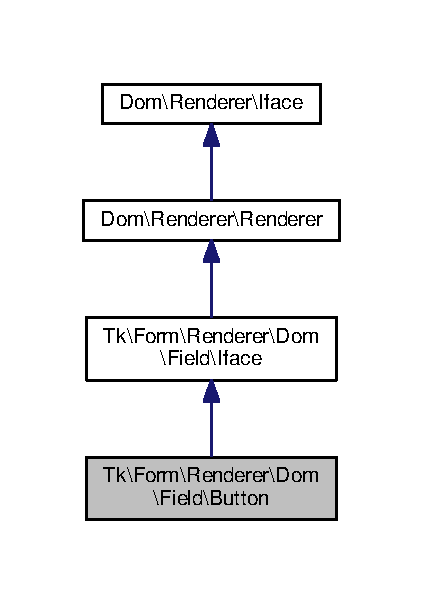
\includegraphics[width=203pt]{classTk_1_1Form_1_1Renderer_1_1Dom_1_1Field_1_1Button__inherit__graph}
\end{center}
\end{figure}
\subsection*{Public Member Functions}
\begin{DoxyCompactItemize}
\item 
\hyperlink{classTk_1_1Form_1_1Renderer_1_1Dom_1_1Field_1_1Button_a7fb360221146282195b769db9ef4d814}{show} ()
\item 
\hyperlink{classTk_1_1Form_1_1Renderer_1_1Dom_1_1Field_1_1Button_ac74be1b42d02fc69baa2ea7b3ff87207}{\+\_\+\+\_\+make\+Template} ()
\end{DoxyCompactItemize}
\subsection*{Additional Inherited Members}


\subsection{Detailed Description}
Class \hyperlink{classTk_1_1Form_1_1Renderer_1_1Dom_1_1Field_1_1Text}{Text}

\begin{DoxyAuthor}{Author}
Michael Mifsud \href{mailto:info@tropotek.com}{\tt info@tropotek.\+com} \hyperlink{}{Copyright 2015 Michael Mifsud }
\end{DoxyAuthor}


\subsection{Member Function Documentation}
\hypertarget{classTk_1_1Form_1_1Renderer_1_1Dom_1_1Field_1_1Button_ac74be1b42d02fc69baa2ea7b3ff87207}{\index{Tk\+::\+Form\+::\+Renderer\+::\+Dom\+::\+Field\+::\+Button@{Tk\+::\+Form\+::\+Renderer\+::\+Dom\+::\+Field\+::\+Button}!\+\_\+\+\_\+make\+Template@{\+\_\+\+\_\+make\+Template}}
\index{\+\_\+\+\_\+make\+Template@{\+\_\+\+\_\+make\+Template}!Tk\+::\+Form\+::\+Renderer\+::\+Dom\+::\+Field\+::\+Button@{Tk\+::\+Form\+::\+Renderer\+::\+Dom\+::\+Field\+::\+Button}}
\subsubsection[{\+\_\+\+\_\+make\+Template}]{\setlength{\rightskip}{0pt plus 5cm}Tk\textbackslash{}\+Form\textbackslash{}\+Renderer\textbackslash{}\+Dom\textbackslash{}\+Field\textbackslash{}\+Button\+::\+\_\+\+\_\+make\+Template (
\begin{DoxyParamCaption}
{}
\end{DoxyParamCaption}
)}}\label{classTk_1_1Form_1_1Renderer_1_1Dom_1_1Field_1_1Button_ac74be1b42d02fc69baa2ea7b3ff87207}
The default element template

\begin{DoxyReturn}{Returns}

\end{DoxyReturn}
\hypertarget{classTk_1_1Form_1_1Renderer_1_1Dom_1_1Field_1_1Button_a7fb360221146282195b769db9ef4d814}{\index{Tk\+::\+Form\+::\+Renderer\+::\+Dom\+::\+Field\+::\+Button@{Tk\+::\+Form\+::\+Renderer\+::\+Dom\+::\+Field\+::\+Button}!show@{show}}
\index{show@{show}!Tk\+::\+Form\+::\+Renderer\+::\+Dom\+::\+Field\+::\+Button@{Tk\+::\+Form\+::\+Renderer\+::\+Dom\+::\+Field\+::\+Button}}
\subsubsection[{show}]{\setlength{\rightskip}{0pt plus 5cm}Tk\textbackslash{}\+Form\textbackslash{}\+Renderer\textbackslash{}\+Dom\textbackslash{}\+Field\textbackslash{}\+Button\+::show (
\begin{DoxyParamCaption}
{}
\end{DoxyParamCaption}
)}}\label{classTk_1_1Form_1_1Renderer_1_1Dom_1_1Field_1_1Button_a7fb360221146282195b769db9ef4d814}
\hyperlink{classTk_1_1Form_1_1Renderer_1_1Dom_1_1Field_1_1Button_a7fb360221146282195b769db9ef4d814}{show()} 

Implements \hyperlink{interfaceDom_1_1Renderer_1_1Iface_a79a0ba41fb6714d69156891d6326bd33}{Dom\textbackslash{}\+Renderer\textbackslash{}\+Iface}.



The documentation for this class was generated from the following file\+:\begin{DoxyCompactItemize}
\item 
vendor/ttek/tk-\/form/\+Tk/\+Form/\+Renderer/\+Dom/\+Field/Button.\+php\end{DoxyCompactItemize}

\hypertarget{classTk_1_1Form_1_1Field_1_1Button}{\section{Tk\textbackslash{}Form\textbackslash{}Field\textbackslash{}Button Class Reference}
\label{classTk_1_1Form_1_1Field_1_1Button}\index{Tk\textbackslash{}\+Form\textbackslash{}\+Field\textbackslash{}\+Button@{Tk\textbackslash{}\+Form\textbackslash{}\+Field\textbackslash{}\+Button}}
}


Inheritance diagram for Tk\textbackslash{}Form\textbackslash{}Field\textbackslash{}Button\+:\nopagebreak
\begin{figure}[H]
\begin{center}
\leavevmode
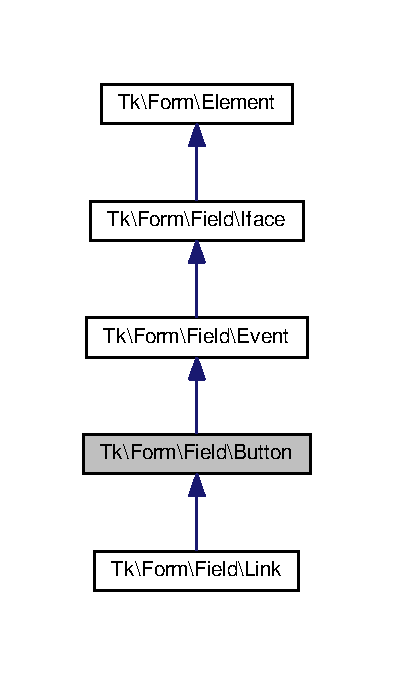
\includegraphics[width=189pt]{classTk_1_1Form_1_1Field_1_1Button__inherit__graph}
\end{center}
\end{figure}
\subsection*{Public Member Functions}
\begin{DoxyCompactItemize}
\item 
\hyperlink{classTk_1_1Form_1_1Field_1_1Button_af4ca506554db2c5e8016624184553b9c}{get\+Icon} ()
\item 
\hyperlink{classTk_1_1Form_1_1Field_1_1Button_ac914a992a73d35809f59f0eb2f2474c9}{set\+Icon} (\$icon)
\end{DoxyCompactItemize}
\subsection*{Protected Attributes}
\begin{DoxyCompactItemize}
\item 
\hypertarget{classTk_1_1Form_1_1Field_1_1Button_a419d000ffa9212a2ab3a6dd54b9015b7}{{\bfseries \$icon} = ''}\label{classTk_1_1Form_1_1Field_1_1Button_a419d000ffa9212a2ab3a6dd54b9015b7}

\end{DoxyCompactItemize}
\subsection*{Additional Inherited Members}


\subsection{Detailed Description}
Class Text

\begin{DoxyAuthor}{Author}
Michael Mifsud \href{mailto:info@tropotek.com}{\tt info@tropotek.\+com} \hyperlink{}{Copyright 2015 Michael Mifsud }
\end{DoxyAuthor}


\subsection{Member Function Documentation}
\hypertarget{classTk_1_1Form_1_1Field_1_1Button_af4ca506554db2c5e8016624184553b9c}{\index{Tk\+::\+Form\+::\+Field\+::\+Button@{Tk\+::\+Form\+::\+Field\+::\+Button}!get\+Icon@{get\+Icon}}
\index{get\+Icon@{get\+Icon}!Tk\+::\+Form\+::\+Field\+::\+Button@{Tk\+::\+Form\+::\+Field\+::\+Button}}
\subsubsection[{get\+Icon}]{\setlength{\rightskip}{0pt plus 5cm}Tk\textbackslash{}\+Form\textbackslash{}\+Field\textbackslash{}\+Button\+::get\+Icon (
\begin{DoxyParamCaption}
{}
\end{DoxyParamCaption}
)}}\label{classTk_1_1Form_1_1Field_1_1Button_af4ca506554db2c5e8016624184553b9c}
\begin{DoxyReturn}{Returns}
string 
\end{DoxyReturn}
\hypertarget{classTk_1_1Form_1_1Field_1_1Button_ac914a992a73d35809f59f0eb2f2474c9}{\index{Tk\+::\+Form\+::\+Field\+::\+Button@{Tk\+::\+Form\+::\+Field\+::\+Button}!set\+Icon@{set\+Icon}}
\index{set\+Icon@{set\+Icon}!Tk\+::\+Form\+::\+Field\+::\+Button@{Tk\+::\+Form\+::\+Field\+::\+Button}}
\subsubsection[{set\+Icon}]{\setlength{\rightskip}{0pt plus 5cm}Tk\textbackslash{}\+Form\textbackslash{}\+Field\textbackslash{}\+Button\+::set\+Icon (
\begin{DoxyParamCaption}
\item[{}]{\$icon}
\end{DoxyParamCaption}
)}}\label{classTk_1_1Form_1_1Field_1_1Button_ac914a992a73d35809f59f0eb2f2474c9}

\begin{DoxyParams}[1]{Parameters}
string & {\em \$icon} & \\
\hline
\end{DoxyParams}
\begin{DoxyReturn}{Returns}
\$this 
\end{DoxyReturn}


The documentation for this class was generated from the following file\+:\begin{DoxyCompactItemize}
\item 
vendor/ttek/tk-\/form/\+Tk/\+Form/\+Field/Button.\+php\end{DoxyCompactItemize}

\hypertarget{classTk_1_1Form_1_1Renderer_1_1Dom_1_1Field_1_1Checkbox}{\section{Tk\textbackslash{}Form\textbackslash{}Renderer\textbackslash{}Dom\textbackslash{}Field\textbackslash{}Checkbox Class Reference}
\label{classTk_1_1Form_1_1Renderer_1_1Dom_1_1Field_1_1Checkbox}\index{Tk\textbackslash{}\+Form\textbackslash{}\+Renderer\textbackslash{}\+Dom\textbackslash{}\+Field\textbackslash{}\+Checkbox@{Tk\textbackslash{}\+Form\textbackslash{}\+Renderer\textbackslash{}\+Dom\textbackslash{}\+Field\textbackslash{}\+Checkbox}}
}


Inheritance diagram for Tk\textbackslash{}Form\textbackslash{}Renderer\textbackslash{}Dom\textbackslash{}Field\textbackslash{}Checkbox\+:\nopagebreak
\begin{figure}[H]
\begin{center}
\leavevmode
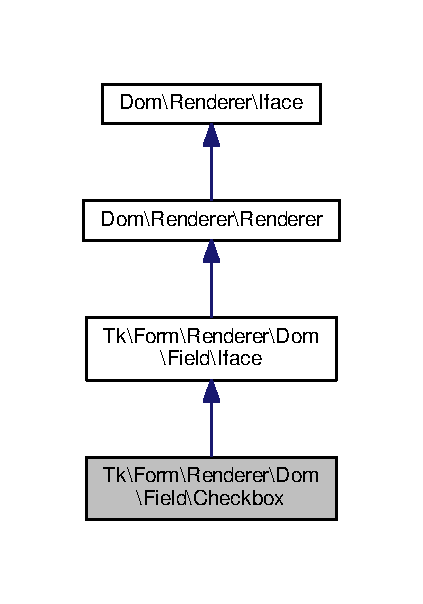
\includegraphics[width=203pt]{classTk_1_1Form_1_1Renderer_1_1Dom_1_1Field_1_1Checkbox__inherit__graph}
\end{center}
\end{figure}
\subsection*{Public Member Functions}
\begin{DoxyCompactItemize}
\item 
\hyperlink{classTk_1_1Form_1_1Renderer_1_1Dom_1_1Field_1_1Checkbox_aeac60284a329e1df6c3699bcb4a39a21}{show\+Element} ()
\item 
\hyperlink{classTk_1_1Form_1_1Renderer_1_1Dom_1_1Field_1_1Checkbox_a5ccb9bccb9c7d208115dca88d4435471}{\+\_\+\+\_\+make\+Template} ()
\end{DoxyCompactItemize}
\subsection*{Additional Inherited Members}


\subsection{Detailed Description}
Class \hyperlink{classTk_1_1Form_1_1Renderer_1_1Dom_1_1Field_1_1Text}{Text}

\begin{DoxyAuthor}{Author}
Michael Mifsud \href{mailto:info@tropotek.com}{\tt info@tropotek.\+com} \hyperlink{}{Copyright 2015 Michael Mifsud }
\end{DoxyAuthor}


\subsection{Member Function Documentation}
\hypertarget{classTk_1_1Form_1_1Renderer_1_1Dom_1_1Field_1_1Checkbox_a5ccb9bccb9c7d208115dca88d4435471}{\index{Tk\+::\+Form\+::\+Renderer\+::\+Dom\+::\+Field\+::\+Checkbox@{Tk\+::\+Form\+::\+Renderer\+::\+Dom\+::\+Field\+::\+Checkbox}!\+\_\+\+\_\+make\+Template@{\+\_\+\+\_\+make\+Template}}
\index{\+\_\+\+\_\+make\+Template@{\+\_\+\+\_\+make\+Template}!Tk\+::\+Form\+::\+Renderer\+::\+Dom\+::\+Field\+::\+Checkbox@{Tk\+::\+Form\+::\+Renderer\+::\+Dom\+::\+Field\+::\+Checkbox}}
\subsubsection[{\+\_\+\+\_\+make\+Template}]{\setlength{\rightskip}{0pt plus 5cm}Tk\textbackslash{}\+Form\textbackslash{}\+Renderer\textbackslash{}\+Dom\textbackslash{}\+Field\textbackslash{}\+Checkbox\+::\+\_\+\+\_\+make\+Template (
\begin{DoxyParamCaption}
{}
\end{DoxyParamCaption}
)}}\label{classTk_1_1Form_1_1Renderer_1_1Dom_1_1Field_1_1Checkbox_a5ccb9bccb9c7d208115dca88d4435471}
The default element template

\begin{DoxyReturn}{Returns}

\end{DoxyReturn}
\hypertarget{classTk_1_1Form_1_1Renderer_1_1Dom_1_1Field_1_1Checkbox_aeac60284a329e1df6c3699bcb4a39a21}{\index{Tk\+::\+Form\+::\+Renderer\+::\+Dom\+::\+Field\+::\+Checkbox@{Tk\+::\+Form\+::\+Renderer\+::\+Dom\+::\+Field\+::\+Checkbox}!show\+Element@{show\+Element}}
\index{show\+Element@{show\+Element}!Tk\+::\+Form\+::\+Renderer\+::\+Dom\+::\+Field\+::\+Checkbox@{Tk\+::\+Form\+::\+Renderer\+::\+Dom\+::\+Field\+::\+Checkbox}}
\subsubsection[{show\+Element}]{\setlength{\rightskip}{0pt plus 5cm}Tk\textbackslash{}\+Form\textbackslash{}\+Renderer\textbackslash{}\+Dom\textbackslash{}\+Field\textbackslash{}\+Checkbox\+::show\+Element (
\begin{DoxyParamCaption}
{}
\end{DoxyParamCaption}
)}}\label{classTk_1_1Form_1_1Renderer_1_1Dom_1_1Field_1_1Checkbox_aeac60284a329e1df6c3699bcb4a39a21}
Render the field and return the template or html string 

The documentation for this class was generated from the following file\+:\begin{DoxyCompactItemize}
\item 
vendor/ttek/tk-\/form/\+Tk/\+Form/\+Renderer/\+Dom/\+Field/Checkbox.\+php\end{DoxyCompactItemize}

\hypertarget{classTk_1_1Table_1_1Cell_1_1Checkbox}{\section{Tk\textbackslash{}Table\textbackslash{}Cell\textbackslash{}Checkbox Class Reference}
\label{classTk_1_1Table_1_1Cell_1_1Checkbox}\index{Tk\textbackslash{}\+Table\textbackslash{}\+Cell\textbackslash{}\+Checkbox@{Tk\textbackslash{}\+Table\textbackslash{}\+Cell\textbackslash{}\+Checkbox}}
}


Inheritance diagram for Tk\textbackslash{}Table\textbackslash{}Cell\textbackslash{}Checkbox\+:\nopagebreak
\begin{figure}[H]
\begin{center}
\leavevmode
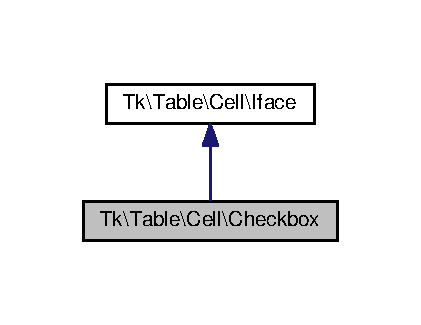
\includegraphics[width=202pt]{classTk_1_1Table_1_1Cell_1_1Checkbox__inherit__graph}
\end{center}
\end{figure}
\subsection*{Public Member Functions}
\begin{DoxyCompactItemize}
\item 
\hyperlink{classTk_1_1Table_1_1Cell_1_1Checkbox_a7e03fa1ce63c9f5fbfae53a76eb085e2}{\+\_\+\+\_\+construct} (\$property)
\item 
\hyperlink{classTk_1_1Table_1_1Cell_1_1Checkbox_afc79af4863df245e7ca21ed950a68a96}{get\+Cell\+Header} ()
\item 
\hyperlink{classTk_1_1Table_1_1Cell_1_1Checkbox_a691981f4df00120dbdd0b80bdde58b39}{get\+Property\+Value} (\$obj, \$property)
\item 
\hyperlink{classTk_1_1Table_1_1Cell_1_1Checkbox_aa8d31b07fe69fc9e042597132911738b}{get\+Cell\+Html} (\$obj)
\end{DoxyCompactItemize}
\subsection*{Additional Inherited Members}


\subsection{Detailed Description}
Class \hyperlink{classTk_1_1Table_1_1Cell_1_1Text}{Text}

\begin{DoxyAuthor}{Author}
Michael Mifsud \href{mailto:info@tropotek.com}{\tt info@tropotek.\+com} \hyperlink{}{Copyright 2015 Michael Mifsud }
\end{DoxyAuthor}


\subsection{Constructor \& Destructor Documentation}
\hypertarget{classTk_1_1Table_1_1Cell_1_1Checkbox_a7e03fa1ce63c9f5fbfae53a76eb085e2}{\index{Tk\+::\+Table\+::\+Cell\+::\+Checkbox@{Tk\+::\+Table\+::\+Cell\+::\+Checkbox}!\+\_\+\+\_\+construct@{\+\_\+\+\_\+construct}}
\index{\+\_\+\+\_\+construct@{\+\_\+\+\_\+construct}!Tk\+::\+Table\+::\+Cell\+::\+Checkbox@{Tk\+::\+Table\+::\+Cell\+::\+Checkbox}}
\subsubsection[{\+\_\+\+\_\+construct}]{\setlength{\rightskip}{0pt plus 5cm}Tk\textbackslash{}\+Table\textbackslash{}\+Cell\textbackslash{}\+Checkbox\+::\+\_\+\+\_\+construct (
\begin{DoxyParamCaption}
\item[{}]{\$property}
\end{DoxyParamCaption}
)}}\label{classTk_1_1Table_1_1Cell_1_1Checkbox_a7e03fa1ce63c9f5fbfae53a76eb085e2}
Create


\begin{DoxyParams}[1]{Parameters}
string & {\em \$property} & \\
\hline
\end{DoxyParams}


\subsection{Member Function Documentation}
\hypertarget{classTk_1_1Table_1_1Cell_1_1Checkbox_afc79af4863df245e7ca21ed950a68a96}{\index{Tk\+::\+Table\+::\+Cell\+::\+Checkbox@{Tk\+::\+Table\+::\+Cell\+::\+Checkbox}!get\+Cell\+Header@{get\+Cell\+Header}}
\index{get\+Cell\+Header@{get\+Cell\+Header}!Tk\+::\+Table\+::\+Cell\+::\+Checkbox@{Tk\+::\+Table\+::\+Cell\+::\+Checkbox}}
\subsubsection[{get\+Cell\+Header}]{\setlength{\rightskip}{0pt plus 5cm}Tk\textbackslash{}\+Table\textbackslash{}\+Cell\textbackslash{}\+Checkbox\+::get\+Cell\+Header (
\begin{DoxyParamCaption}
{}
\end{DoxyParamCaption}
)}}\label{classTk_1_1Table_1_1Cell_1_1Checkbox_afc79af4863df245e7ca21ed950a68a96}
\begin{DoxyReturn}{Returns}
string 
\end{DoxyReturn}
\hypertarget{classTk_1_1Table_1_1Cell_1_1Checkbox_aa8d31b07fe69fc9e042597132911738b}{\index{Tk\+::\+Table\+::\+Cell\+::\+Checkbox@{Tk\+::\+Table\+::\+Cell\+::\+Checkbox}!get\+Cell\+Html@{get\+Cell\+Html}}
\index{get\+Cell\+Html@{get\+Cell\+Html}!Tk\+::\+Table\+::\+Cell\+::\+Checkbox@{Tk\+::\+Table\+::\+Cell\+::\+Checkbox}}
\subsubsection[{get\+Cell\+Html}]{\setlength{\rightskip}{0pt plus 5cm}Tk\textbackslash{}\+Table\textbackslash{}\+Cell\textbackslash{}\+Checkbox\+::get\+Cell\+Html (
\begin{DoxyParamCaption}
\item[{}]{\$obj}
\end{DoxyParamCaption}
)}}\label{classTk_1_1Table_1_1Cell_1_1Checkbox_aa8d31b07fe69fc9e042597132911738b}

\begin{DoxyParams}[1]{Parameters}
mixed & {\em \$obj} & \\
\hline
\end{DoxyParams}
\begin{DoxyReturn}{Returns}
string 
\end{DoxyReturn}
\hypertarget{classTk_1_1Table_1_1Cell_1_1Checkbox_a691981f4df00120dbdd0b80bdde58b39}{\index{Tk\+::\+Table\+::\+Cell\+::\+Checkbox@{Tk\+::\+Table\+::\+Cell\+::\+Checkbox}!get\+Property\+Value@{get\+Property\+Value}}
\index{get\+Property\+Value@{get\+Property\+Value}!Tk\+::\+Table\+::\+Cell\+::\+Checkbox@{Tk\+::\+Table\+::\+Cell\+::\+Checkbox}}
\subsubsection[{get\+Property\+Value}]{\setlength{\rightskip}{0pt plus 5cm}Tk\textbackslash{}\+Table\textbackslash{}\+Cell\textbackslash{}\+Checkbox\+::get\+Property\+Value (
\begin{DoxyParamCaption}
\item[{}]{\$obj, }
\item[{}]{\$property}
\end{DoxyParamCaption}
)}}\label{classTk_1_1Table_1_1Cell_1_1Checkbox_a691981f4df00120dbdd0b80bdde58b39}
Get the property value from the object This should be the clean property data with no H\+T\+M\+L or rendering attached, unless the rendering code is part of the value as it will be called for outputting to other files like X\+M\+L or C\+S\+V.


\begin{DoxyParams}[1]{Parameters}
object & {\em \$obj} & \\
\hline
string & {\em \$property} & \\
\hline
\end{DoxyParams}
\begin{DoxyReturn}{Returns}
mixed 
\end{DoxyReturn}


The documentation for this class was generated from the following file\+:\begin{DoxyCompactItemize}
\item 
vendor/ttek/tk-\/table/\+Tk/\+Table/\+Cell/Checkbox.\+php\end{DoxyCompactItemize}

\hypertarget{classTk_1_1Form_1_1Field_1_1Checkbox}{\section{Tk\textbackslash{}Form\textbackslash{}Field\textbackslash{}Checkbox Class Reference}
\label{classTk_1_1Form_1_1Field_1_1Checkbox}\index{Tk\textbackslash{}\+Form\textbackslash{}\+Field\textbackslash{}\+Checkbox@{Tk\textbackslash{}\+Form\textbackslash{}\+Field\textbackslash{}\+Checkbox}}
}


Inheritance diagram for Tk\textbackslash{}Form\textbackslash{}Field\textbackslash{}Checkbox\+:\nopagebreak
\begin{figure}[H]
\begin{center}
\leavevmode
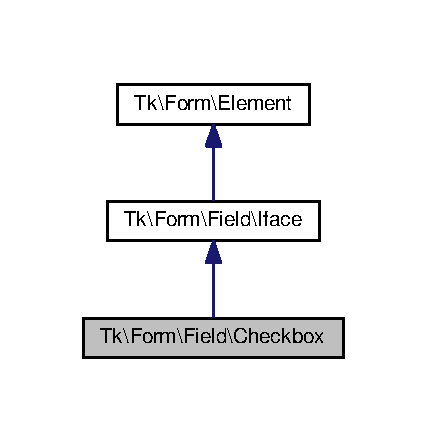
\includegraphics[width=205pt]{classTk_1_1Form_1_1Field_1_1Checkbox__inherit__graph}
\end{center}
\end{figure}
\subsection*{Public Member Functions}
\begin{DoxyCompactItemize}
\item 
\hyperlink{classTk_1_1Form_1_1Field_1_1Checkbox_a6a9f8db23e043e57d5f04cced6a9bfc6}{is\+Checked} ()
\end{DoxyCompactItemize}
\subsection*{Additional Inherited Members}


\subsection{Detailed Description}
Class Text

\begin{DoxyAuthor}{Author}
Michael Mifsud \href{mailto:info@tropotek.com}{\tt info@tropotek.\+com} \hyperlink{}{Copyright 2015 Michael Mifsud }
\end{DoxyAuthor}


\subsection{Member Function Documentation}
\hypertarget{classTk_1_1Form_1_1Field_1_1Checkbox_a6a9f8db23e043e57d5f04cced6a9bfc6}{\index{Tk\+::\+Form\+::\+Field\+::\+Checkbox@{Tk\+::\+Form\+::\+Field\+::\+Checkbox}!is\+Checked@{is\+Checked}}
\index{is\+Checked@{is\+Checked}!Tk\+::\+Form\+::\+Field\+::\+Checkbox@{Tk\+::\+Form\+::\+Field\+::\+Checkbox}}
\subsubsection[{is\+Checked}]{\setlength{\rightskip}{0pt plus 5cm}Tk\textbackslash{}\+Form\textbackslash{}\+Field\textbackslash{}\+Checkbox\+::is\+Checked (
\begin{DoxyParamCaption}
{}
\end{DoxyParamCaption}
)}}\label{classTk_1_1Form_1_1Field_1_1Checkbox_a6a9f8db23e043e57d5f04cced6a9bfc6}
Is the value checked

\begin{DoxyReturn}{Returns}
bool 
\end{DoxyReturn}


The documentation for this class was generated from the following file\+:\begin{DoxyCompactItemize}
\item 
vendor/ttek/tk-\/form/\+Tk/\+Form/\+Field/Checkbox.\+php\end{DoxyCompactItemize}

\hypertarget{classDom_1_1Loader_1_1Adapter_1_1ClassPath}{\section{Dom\textbackslash{}Loader\textbackslash{}Adapter\textbackslash{}Class\+Path Class Reference}
\label{classDom_1_1Loader_1_1Adapter_1_1ClassPath}\index{Dom\textbackslash{}\+Loader\textbackslash{}\+Adapter\textbackslash{}\+Class\+Path@{Dom\textbackslash{}\+Loader\textbackslash{}\+Adapter\textbackslash{}\+Class\+Path}}
}


Inheritance diagram for Dom\textbackslash{}Loader\textbackslash{}Adapter\textbackslash{}Class\+Path\+:\nopagebreak
\begin{figure}[H]
\begin{center}
\leavevmode
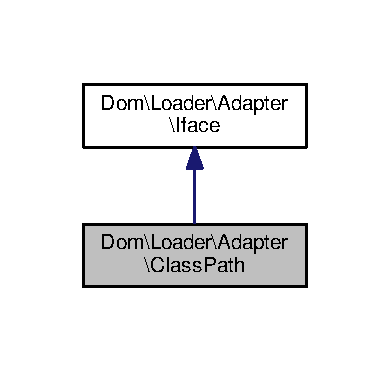
\includegraphics[width=187pt]{classDom_1_1Loader_1_1Adapter_1_1ClassPath__inherit__graph}
\end{center}
\end{figure}
\subsection*{Public Member Functions}
\begin{DoxyCompactItemize}
\item 
\hyperlink{classDom_1_1Loader_1_1Adapter_1_1ClassPath_a2318a0e91b0fdb17ed11607422606488}{\+\_\+\+\_\+construct} (\$path, \$ext= 'xml')
\item 
\hyperlink{classDom_1_1Loader_1_1Adapter_1_1ClassPath_a3a166e4fefe892ff9caee266167fbb0b}{load} (\$xhtml, \$class)
\item 
\hyperlink{classDom_1_1Loader_1_1Adapter_1_1ClassPath_a16057826d74de740beb56b4d73dc0b79}{load\+File} (\$path, \$class)
\end{DoxyCompactItemize}
\subsection*{Protected Attributes}
\begin{DoxyCompactItemize}
\item 
\hypertarget{classDom_1_1Loader_1_1Adapter_1_1ClassPath_a5dc4e61c70034b98e942f750b10cabb5}{{\bfseries \$ext} = ''}\label{classDom_1_1Loader_1_1Adapter_1_1ClassPath_a5dc4e61c70034b98e942f750b10cabb5}

\item 
\hypertarget{classDom_1_1Loader_1_1Adapter_1_1ClassPath_a33f2500c4eca9812a56562ee26dbbdb6}{{\bfseries \$path} = ''}\label{classDom_1_1Loader_1_1Adapter_1_1ClassPath_a33f2500c4eca9812a56562ee26dbbdb6}

\end{DoxyCompactItemize}


\subsection{Detailed Description}
This adapter will look for template files in the supplied paths using the class name with underscores

For example\+: if the supplied class is  The class is converted to App\+\_\+\+Module\+\_\+\+Index The adapter will look for a template in the supplied path for example\+: /supplied/template/path/\+App\+\_\+\+Module\+\_\+\+Index.xml

\begin{DoxyAuthor}{Author}
Michael Mifsud \href{mailto:info@tropotek.com}{\tt info@tropotek.\+com} \hyperlink{}{Copyright 2015 Michael Mifsud }
\end{DoxyAuthor}


\subsection{Constructor \& Destructor Documentation}
\hypertarget{classDom_1_1Loader_1_1Adapter_1_1ClassPath_a2318a0e91b0fdb17ed11607422606488}{\index{Dom\+::\+Loader\+::\+Adapter\+::\+Class\+Path@{Dom\+::\+Loader\+::\+Adapter\+::\+Class\+Path}!\+\_\+\+\_\+construct@{\+\_\+\+\_\+construct}}
\index{\+\_\+\+\_\+construct@{\+\_\+\+\_\+construct}!Dom\+::\+Loader\+::\+Adapter\+::\+Class\+Path@{Dom\+::\+Loader\+::\+Adapter\+::\+Class\+Path}}
\subsubsection[{\+\_\+\+\_\+construct}]{\setlength{\rightskip}{0pt plus 5cm}Dom\textbackslash{}\+Loader\textbackslash{}\+Adapter\textbackslash{}\+Class\+Path\+::\+\_\+\+\_\+construct (
\begin{DoxyParamCaption}
\item[{}]{\$path, }
\item[{}]{\$ext = {\ttfamily 'xml'}}
\end{DoxyParamCaption}
)}}\label{classDom_1_1Loader_1_1Adapter_1_1ClassPath_a2318a0e91b0fdb17ed11607422606488}

\begin{DoxyParams}[1]{Parameters}
array & {\em \$path} & The path to the template folder \\
\hline
string & {\em \$ext} & The template file extension, default 'xml' \\
\hline
\end{DoxyParams}


\subsection{Member Function Documentation}
\hypertarget{classDom_1_1Loader_1_1Adapter_1_1ClassPath_a3a166e4fefe892ff9caee266167fbb0b}{\index{Dom\+::\+Loader\+::\+Adapter\+::\+Class\+Path@{Dom\+::\+Loader\+::\+Adapter\+::\+Class\+Path}!load@{load}}
\index{load@{load}!Dom\+::\+Loader\+::\+Adapter\+::\+Class\+Path@{Dom\+::\+Loader\+::\+Adapter\+::\+Class\+Path}}
\subsubsection[{load}]{\setlength{\rightskip}{0pt plus 5cm}Dom\textbackslash{}\+Loader\textbackslash{}\+Adapter\textbackslash{}\+Class\+Path\+::load (
\begin{DoxyParamCaption}
\item[{}]{\$xhtml, }
\item[{}]{\$class}
\end{DoxyParamCaption}
)}}\label{classDom_1_1Loader_1_1Adapter_1_1ClassPath_a3a166e4fefe892ff9caee266167fbb0b}
Load an xml/xhtml strings


\begin{DoxyParams}{Parameters}
{\em \$xhtml} & \\
\hline
{\em \$class} & \\
\hline
\end{DoxyParams}
\begin{DoxyReturn}{Returns}
\hyperlink{classDom_1_1Template}{Template} 
\end{DoxyReturn}
\hypertarget{classDom_1_1Loader_1_1Adapter_1_1ClassPath_a16057826d74de740beb56b4d73dc0b79}{\index{Dom\+::\+Loader\+::\+Adapter\+::\+Class\+Path@{Dom\+::\+Loader\+::\+Adapter\+::\+Class\+Path}!load\+File@{load\+File}}
\index{load\+File@{load\+File}!Dom\+::\+Loader\+::\+Adapter\+::\+Class\+Path@{Dom\+::\+Loader\+::\+Adapter\+::\+Class\+Path}}
\subsubsection[{load\+File}]{\setlength{\rightskip}{0pt plus 5cm}Dom\textbackslash{}\+Loader\textbackslash{}\+Adapter\textbackslash{}\+Class\+Path\+::load\+File (
\begin{DoxyParamCaption}
\item[{}]{\$path, }
\item[{}]{\$class}
\end{DoxyParamCaption}
)}}\label{classDom_1_1Loader_1_1Adapter_1_1ClassPath_a16057826d74de740beb56b4d73dc0b79}
Load an xml/xhtml file


\begin{DoxyParams}{Parameters}
{\em \$path} & \\
\hline
{\em \$class} & \\
\hline
\end{DoxyParams}
\begin{DoxyReturn}{Returns}
\hyperlink{classDom_1_1Template}{Template} 
\end{DoxyReturn}


The documentation for this class was generated from the following file\+:\begin{DoxyCompactItemize}
\item 
vendor/ttek/tk-\/domtemplate/\+Dom/\+Loader/\+Adapter/Class\+Path.\+php\end{DoxyCompactItemize}

\hypertarget{classTk_1_1Util_1_1ClassTools}{\section{Tk\textbackslash{}Util\textbackslash{}Class\+Tools Class Reference}
\label{classTk_1_1Util_1_1ClassTools}\index{Tk\textbackslash{}\+Util\textbackslash{}\+Class\+Tools@{Tk\textbackslash{}\+Util\textbackslash{}\+Class\+Tools}}
}
\subsection*{Static Public Member Functions}
\begin{DoxyCompactItemize}
\item 
static \hyperlink{classTk_1_1Util_1_1ClassTools_a6ce79620ab530df1c8f3572a7253e3a7}{to\+Namespace\+Slash} (\$class)
\item 
static \hyperlink{classTk_1_1Util_1_1ClassTools_abc3d69f19657b5251674dfc8d91f1862}{to\+Namespace\+Underscore} (\$class)
\item 
static \hyperlink{classTk_1_1Util_1_1ClassTools_a3588c393f1d315f30a8bc38884c577e4}{classpath} (\$class)
\item 
static \hyperlink{classTk_1_1Util_1_1ClassTools_afb9242d982061d8daf00f939f49fee43}{class\+Url} (\$class)
\end{DoxyCompactItemize}


\subsection{Member Function Documentation}
\hypertarget{classTk_1_1Util_1_1ClassTools_a3588c393f1d315f30a8bc38884c577e4}{\index{Tk\+::\+Util\+::\+Class\+Tools@{Tk\+::\+Util\+::\+Class\+Tools}!classpath@{classpath}}
\index{classpath@{classpath}!Tk\+::\+Util\+::\+Class\+Tools@{Tk\+::\+Util\+::\+Class\+Tools}}
\subsubsection[{classpath}]{\setlength{\rightskip}{0pt plus 5cm}static Tk\textbackslash{}\+Util\textbackslash{}\+Class\+Tools\+::classpath (
\begin{DoxyParamCaption}
\item[{}]{\$class}
\end{DoxyParamCaption}
)\hspace{0.3cm}{\ttfamily [static]}}}\label{classTk_1_1Util_1_1ClassTools_a3588c393f1d315f30a8bc38884c577e4}
Get the path of a class


\begin{DoxyParams}[1]{Parameters}
string | Object & {\em \$class} & \\
\hline
\end{DoxyParams}
\begin{DoxyReturn}{Returns}
string 
\end{DoxyReturn}
\hypertarget{classTk_1_1Util_1_1ClassTools_afb9242d982061d8daf00f939f49fee43}{\index{Tk\+::\+Util\+::\+Class\+Tools@{Tk\+::\+Util\+::\+Class\+Tools}!class\+Url@{class\+Url}}
\index{class\+Url@{class\+Url}!Tk\+::\+Util\+::\+Class\+Tools@{Tk\+::\+Util\+::\+Class\+Tools}}
\subsubsection[{class\+Url}]{\setlength{\rightskip}{0pt plus 5cm}static Tk\textbackslash{}\+Util\textbackslash{}\+Class\+Tools\+::class\+Url (
\begin{DoxyParamCaption}
\item[{}]{\$class}
\end{DoxyParamCaption}
)\hspace{0.3cm}{\ttfamily [static]}}}\label{classTk_1_1Util_1_1ClassTools_afb9242d982061d8daf00f939f49fee43}
Get the url path of a class


\begin{DoxyParams}[1]{Parameters}
string | Object & {\em \$class} & \\
\hline
\end{DoxyParams}
\begin{DoxyReturn}{Returns}
string 
\end{DoxyReturn}
\hypertarget{classTk_1_1Util_1_1ClassTools_a6ce79620ab530df1c8f3572a7253e3a7}{\index{Tk\+::\+Util\+::\+Class\+Tools@{Tk\+::\+Util\+::\+Class\+Tools}!to\+Namespace\+Slash@{to\+Namespace\+Slash}}
\index{to\+Namespace\+Slash@{to\+Namespace\+Slash}!Tk\+::\+Util\+::\+Class\+Tools@{Tk\+::\+Util\+::\+Class\+Tools}}
\subsubsection[{to\+Namespace\+Slash}]{\setlength{\rightskip}{0pt plus 5cm}static Tk\textbackslash{}\+Util\textbackslash{}\+Class\+Tools\+::to\+Namespace\+Slash (
\begin{DoxyParamCaption}
\item[{}]{\$class}
\end{DoxyParamCaption}
)\hspace{0.3cm}{\ttfamily [static]}}}\label{classTk_1_1Util_1_1ClassTools_a6ce79620ab530df1c8f3572a7253e3a7}
Take a class in the form of Tk\+\_\+\+Some\+\_\+\+Class And convert it to a class like 


\begin{DoxyParams}[1]{Parameters}
string & {\em \$class} & \\
\hline
\end{DoxyParams}
\begin{DoxyReturn}{Returns}
string 
\end{DoxyReturn}
\hypertarget{classTk_1_1Util_1_1ClassTools_abc3d69f19657b5251674dfc8d91f1862}{\index{Tk\+::\+Util\+::\+Class\+Tools@{Tk\+::\+Util\+::\+Class\+Tools}!to\+Namespace\+Underscore@{to\+Namespace\+Underscore}}
\index{to\+Namespace\+Underscore@{to\+Namespace\+Underscore}!Tk\+::\+Util\+::\+Class\+Tools@{Tk\+::\+Util\+::\+Class\+Tools}}
\subsubsection[{to\+Namespace\+Underscore}]{\setlength{\rightskip}{0pt plus 5cm}static Tk\textbackslash{}\+Util\textbackslash{}\+Class\+Tools\+::to\+Namespace\+Underscore (
\begin{DoxyParamCaption}
\item[{}]{\$class}
\end{DoxyParamCaption}
)\hspace{0.3cm}{\ttfamily [static]}}}\label{classTk_1_1Util_1_1ClassTools_abc3d69f19657b5251674dfc8d91f1862}
Take a class in the form of  And convert it to a namespace class like Tk\+\_\+\+Some\+\_\+\+Class


\begin{DoxyParams}[1]{Parameters}
string & {\em \$class} & \\
\hline
\end{DoxyParams}
\begin{DoxyReturn}{Returns}
string 
\end{DoxyReturn}


The documentation for this class was generated from the following file\+:\begin{DoxyCompactItemize}
\item 
vendor/ttek/tk-\/framework/\+Tk/\+Util/Class\+Tools.\+php\end{DoxyCompactItemize}

\hypertarget{classTk_1_1Config}{\section{Tk\textbackslash{}Config Class Reference}
\label{classTk_1_1Config}\index{Tk\textbackslash{}\+Config@{Tk\textbackslash{}\+Config}}
}


Inheritance diagram for Tk\textbackslash{}Config\+:\nopagebreak
\begin{figure}[H]
\begin{center}
\leavevmode
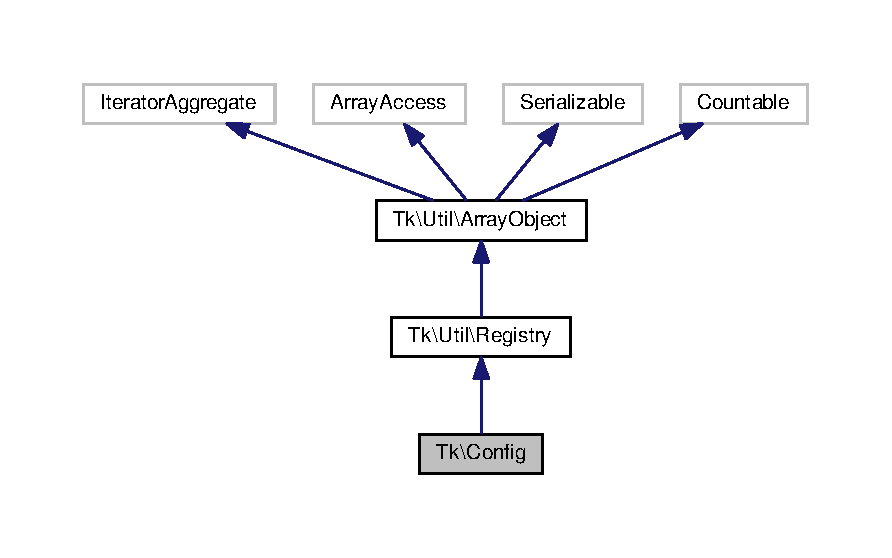
\includegraphics[width=350pt]{classTk_1_1Config__inherit__graph}
\end{center}
\end{figure}
\subsection*{Public Member Functions}
\begin{DoxyCompactItemize}
\item 
\hyperlink{classTk_1_1Config_ae330d7a7e50597ab4b06e9713b2e629c}{\+\_\+\+\_\+construct} (\$app\+Url= '', \$app\+Path= '')
\item 
\hyperlink{classTk_1_1Config_aaf64cfba50af0da87adcee508253d652}{get\+App\+Url} ()
\item 
\hyperlink{classTk_1_1Config_a663d12fd13dd70777756cff67001b43d}{get\+App\+Path} ()
\item 
\hyperlink{classTk_1_1Config_ac7fab993eb970174b662639954132b2c}{get\+Data\+Url} ()
\item 
\hyperlink{classTk_1_1Config_a194ce70e71e59431958662ce932e57da}{get\+Data\+Path} ()
\item 
\hyperlink{classTk_1_1Config_aab2a6666aee90ed5bd9805f44894ef69}{get\+Vendor\+Url} ()
\item 
\hyperlink{classTk_1_1Config_ae8ed66cab17c82847c779f1356a26555}{get\+Vendor\+Path} ()
\item 
\hyperlink{classTk_1_1Config_a6dfe526acbc3299db77e9251deb731d5}{get\+Src\+Url} ()
\item 
\hyperlink{classTk_1_1Config_ad214878dbfdeeaca36c876c17c3b7cfe}{get\+Src\+Path} ()
\item 
\hyperlink{classTk_1_1Config_adff63f0d8c8b5ac24395edae3a6ab364}{get\+Cache\+Url} ()
\item 
\hyperlink{classTk_1_1Config_a5cd69177657c4eec63a981bceb3c8208}{get\+Cache\+Path} ()
\item 
\hyperlink{classTk_1_1Config_a89a075190ce0e61460a0e0e087eeaa94}{get\+Temp\+Url} ()
\item 
\hyperlink{classTk_1_1Config_a9c8429bc4389ec667da5a5d36c9eeb40}{get\+Temp\+Path} ()
\item 
\hyperlink{classTk_1_1Config_aa37ded1aff99203676dbcba44a9c5b26}{get\+Cli} ()
\end{DoxyCompactItemize}
\subsection*{Static Public Member Functions}
\begin{DoxyCompactItemize}
\item 
static \hyperlink{classTk_1_1Config_a3bff1684d5e067d86e4874c81ec1a69a}{get\+Instance} (\$app\+Url= '', \$app\+Path= '')
\end{DoxyCompactItemize}
\subsection*{Static Public Attributes}
\begin{DoxyCompactItemize}
\item 
\hypertarget{classTk_1_1Config_a72790ffe560d691c3d411c0102974a3c}{static {\bfseries \$instance} = null}\label{classTk_1_1Config_a72790ffe560d691c3d411c0102974a3c}

\end{DoxyCompactItemize}
\subsection*{Protected Member Functions}
\begin{DoxyCompactItemize}
\item 
\hyperlink{classTk_1_1Config_adaf29d4b83d6ed431da8bef0bd454b92}{init} (\$app\+Url= '', \$app\+Path= '')
\end{DoxyCompactItemize}


\subsection{Detailed Description}
A \hyperlink{classTk_1_1Config}{Config} class for handling the applications dependency values.

It can be used as a standard array it extends the  Example usage\+: 
\begin{DoxyCode}
$request = Request::createFromGlobals();
$cfg = \hyperlink{classTk_1_1Config_a3bff1684d5e067d86e4874c81ec1a69a}{\(\backslash\)Tk\(\backslash\)Config::getInstance}();

$cfg->setAppPath($appPath);
$cfg->setRequest($request);
$cfg->setAppUrl($request->getBasePath());
$cfg->setAppDataPath($cfg->getAppPath().\textcolor{stringliteral}{'/data'});
$cfg->setAppCachePath($cfg->getAppDataPath().\textcolor{stringliteral}{'/cache'});
$cfg->setAppTempPath($cfg->getAppDataPath().\textcolor{stringliteral}{'/temp'});
\textcolor{comment}{// Useful for dependency management to create application objects}
$cfg->setStdObject(\textcolor{keyword}{function}($test1, $test2, $test3) \{
    $cfg = \(\backslash\)Tk\(\backslash\)Registry::getInstance();
    $obj = new \(\backslash\)stdClass();
    $obj->test1 = $test1;
    $obj->test2 = $test1;
    $obj->test3 = $test1;
    \textcolor{keywordflow}{return} $obj;
\});

$var = $cfg->getStdObject(\textcolor{stringliteral}{'test param'}, \textcolor{stringliteral}{'test2'}, \textcolor{stringliteral}{'test3'});
\textcolor{comment}{// or}
$var = $cfg->createStdObject(\textcolor{stringliteral}{'test param'}, \textcolor{stringliteral}{'test2'}, \textcolor{stringliteral}{'test3'});
\textcolor{comment}{// or}
$var = $cfg->isStdObject(\textcolor{stringliteral}{'test param'}, \textcolor{stringliteral}{'test2'}, \textcolor{stringliteral}{'test3'});
var\_dump($var);


 \textcolor{comment}{// Output:}
 \textcolor{comment}{//  object(stdClass)[15]}
 \textcolor{comment}{//      public 'test1' => string 'test param' (length=10)}
 \textcolor{comment}{//      public 'test2' => string 'test param' (length=10)}
 \textcolor{comment}{//      public 'test3' => string 'test param' (length=10)}

 \textcolor{comment}{// The following returns the closure object not the result}

$var = $cfg->get(\textcolor{stringliteral}{'std.object'});
var\_dump($var);

\textcolor{comment}{// Output}
\textcolor{comment}{// object(Closure)[14]}
\end{DoxyCode}


Internally the \hyperlink{classTk_1_1Config}{Config} values are stored in an array. So to set a value there is a couple of ways to do this\+:


\begin{DoxyCode}
$cfg->setSitePath($path);
\end{DoxyCode}


same as


\begin{DoxyCode}
$cfg[\textcolor{stringliteral}{'site.path'}] = $path;
\end{DoxyCode}


To get a values stored in the registry you can do the following using the array access methods\+:


\begin{DoxyCode}
$val = $cfg->getSitePath();
\end{DoxyCode}


same as


\begin{DoxyCode}
$val = $cfg[\textcolor{stringliteral}{'site.path'}];
\end{DoxyCode}


\begin{DoxyAuthor}{Author}
Michael Mifsud \href{mailto:info@tropotek.com}{\tt info@tropotek.\+com} \hyperlink{}{Copyright 2007 Michael Mifsud }
\end{DoxyAuthor}


\subsection{Constructor \& Destructor Documentation}
\hypertarget{classTk_1_1Config_ae330d7a7e50597ab4b06e9713b2e629c}{\index{Tk\+::\+Config@{Tk\+::\+Config}!\+\_\+\+\_\+construct@{\+\_\+\+\_\+construct}}
\index{\+\_\+\+\_\+construct@{\+\_\+\+\_\+construct}!Tk\+::\+Config@{Tk\+::\+Config}}
\subsubsection[{\+\_\+\+\_\+construct}]{\setlength{\rightskip}{0pt plus 5cm}Tk\textbackslash{}\+Config\+::\+\_\+\+\_\+construct (
\begin{DoxyParamCaption}
\item[{}]{\$app\+Url = {\ttfamily ''}, }
\item[{}]{\$app\+Path = {\ttfamily ''}}
\end{DoxyParamCaption}
)}}\label{classTk_1_1Config_ae330d7a7e50597ab4b06e9713b2e629c}
Construct the config object and initiate default settings


\begin{DoxyParams}[1]{Parameters}
string & {\em \$app\+Url} & \\
\hline
string & {\em \$app\+Path} & \\
\hline
\end{DoxyParams}


\subsection{Member Function Documentation}
\hypertarget{classTk_1_1Config_a663d12fd13dd70777756cff67001b43d}{\index{Tk\+::\+Config@{Tk\+::\+Config}!get\+App\+Path@{get\+App\+Path}}
\index{get\+App\+Path@{get\+App\+Path}!Tk\+::\+Config@{Tk\+::\+Config}}
\subsubsection[{get\+App\+Path}]{\setlength{\rightskip}{0pt plus 5cm}Tk\textbackslash{}\+Config\+::get\+App\+Path (
\begin{DoxyParamCaption}
{}
\end{DoxyParamCaption}
)}}\label{classTk_1_1Config_a663d12fd13dd70777756cff67001b43d}
\begin{DoxyReturn}{Returns}
string 
\end{DoxyReturn}
\hypertarget{classTk_1_1Config_aaf64cfba50af0da87adcee508253d652}{\index{Tk\+::\+Config@{Tk\+::\+Config}!get\+App\+Url@{get\+App\+Url}}
\index{get\+App\+Url@{get\+App\+Url}!Tk\+::\+Config@{Tk\+::\+Config}}
\subsubsection[{get\+App\+Url}]{\setlength{\rightskip}{0pt plus 5cm}Tk\textbackslash{}\+Config\+::get\+App\+Url (
\begin{DoxyParamCaption}
{}
\end{DoxyParamCaption}
)}}\label{classTk_1_1Config_aaf64cfba50af0da87adcee508253d652}
\begin{DoxyReturn}{Returns}
string 
\end{DoxyReturn}
\hypertarget{classTk_1_1Config_a5cd69177657c4eec63a981bceb3c8208}{\index{Tk\+::\+Config@{Tk\+::\+Config}!get\+Cache\+Path@{get\+Cache\+Path}}
\index{get\+Cache\+Path@{get\+Cache\+Path}!Tk\+::\+Config@{Tk\+::\+Config}}
\subsubsection[{get\+Cache\+Path}]{\setlength{\rightskip}{0pt plus 5cm}Tk\textbackslash{}\+Config\+::get\+Cache\+Path (
\begin{DoxyParamCaption}
{}
\end{DoxyParamCaption}
)}}\label{classTk_1_1Config_a5cd69177657c4eec63a981bceb3c8208}
\begin{DoxyReturn}{Returns}
string 
\end{DoxyReturn}
\hypertarget{classTk_1_1Config_adff63f0d8c8b5ac24395edae3a6ab364}{\index{Tk\+::\+Config@{Tk\+::\+Config}!get\+Cache\+Url@{get\+Cache\+Url}}
\index{get\+Cache\+Url@{get\+Cache\+Url}!Tk\+::\+Config@{Tk\+::\+Config}}
\subsubsection[{get\+Cache\+Url}]{\setlength{\rightskip}{0pt plus 5cm}Tk\textbackslash{}\+Config\+::get\+Cache\+Url (
\begin{DoxyParamCaption}
{}
\end{DoxyParamCaption}
)}}\label{classTk_1_1Config_adff63f0d8c8b5ac24395edae3a6ab364}
\begin{DoxyReturn}{Returns}
string 
\end{DoxyReturn}
\hypertarget{classTk_1_1Config_aa37ded1aff99203676dbcba44a9c5b26}{\index{Tk\+::\+Config@{Tk\+::\+Config}!get\+Cli@{get\+Cli}}
\index{get\+Cli@{get\+Cli}!Tk\+::\+Config@{Tk\+::\+Config}}
\subsubsection[{get\+Cli}]{\setlength{\rightskip}{0pt plus 5cm}Tk\textbackslash{}\+Config\+::get\+Cli (
\begin{DoxyParamCaption}
{}
\end{DoxyParamCaption}
)}}\label{classTk_1_1Config_aa37ded1aff99203676dbcba44a9c5b26}
Is this application a command run in a terminal \begin{DoxyReturn}{Returns}
boolean 
\end{DoxyReturn}
\hypertarget{classTk_1_1Config_a194ce70e71e59431958662ce932e57da}{\index{Tk\+::\+Config@{Tk\+::\+Config}!get\+Data\+Path@{get\+Data\+Path}}
\index{get\+Data\+Path@{get\+Data\+Path}!Tk\+::\+Config@{Tk\+::\+Config}}
\subsubsection[{get\+Data\+Path}]{\setlength{\rightskip}{0pt plus 5cm}Tk\textbackslash{}\+Config\+::get\+Data\+Path (
\begin{DoxyParamCaption}
{}
\end{DoxyParamCaption}
)}}\label{classTk_1_1Config_a194ce70e71e59431958662ce932e57da}
\begin{DoxyReturn}{Returns}
string 
\end{DoxyReturn}
\hypertarget{classTk_1_1Config_ac7fab993eb970174b662639954132b2c}{\index{Tk\+::\+Config@{Tk\+::\+Config}!get\+Data\+Url@{get\+Data\+Url}}
\index{get\+Data\+Url@{get\+Data\+Url}!Tk\+::\+Config@{Tk\+::\+Config}}
\subsubsection[{get\+Data\+Url}]{\setlength{\rightskip}{0pt plus 5cm}Tk\textbackslash{}\+Config\+::get\+Data\+Url (
\begin{DoxyParamCaption}
{}
\end{DoxyParamCaption}
)}}\label{classTk_1_1Config_ac7fab993eb970174b662639954132b2c}
\begin{DoxyReturn}{Returns}
string 
\end{DoxyReturn}
\hypertarget{classTk_1_1Config_a3bff1684d5e067d86e4874c81ec1a69a}{\index{Tk\+::\+Config@{Tk\+::\+Config}!get\+Instance@{get\+Instance}}
\index{get\+Instance@{get\+Instance}!Tk\+::\+Config@{Tk\+::\+Config}}
\subsubsection[{get\+Instance}]{\setlength{\rightskip}{0pt plus 5cm}static Tk\textbackslash{}\+Config\+::get\+Instance (
\begin{DoxyParamCaption}
\item[{}]{\$app\+Url = {\ttfamily ''}, }
\item[{}]{\$app\+Path = {\ttfamily ''}}
\end{DoxyParamCaption}
)\hspace{0.3cm}{\ttfamily [static]}}}\label{classTk_1_1Config_a3bff1684d5e067d86e4874c81ec1a69a}
Get an instance of this object


\begin{DoxyParams}[1]{Parameters}
string & {\em \$app\+Url} & Only required on first call to init the config paths \\
\hline
string & {\em \$app\+Path} & \\
\hline
\end{DoxyParams}
\begin{DoxyReturn}{Returns}
\hyperlink{classTk_1_1Config}{Config} 
\end{DoxyReturn}
\hypertarget{classTk_1_1Config_ad214878dbfdeeaca36c876c17c3b7cfe}{\index{Tk\+::\+Config@{Tk\+::\+Config}!get\+Src\+Path@{get\+Src\+Path}}
\index{get\+Src\+Path@{get\+Src\+Path}!Tk\+::\+Config@{Tk\+::\+Config}}
\subsubsection[{get\+Src\+Path}]{\setlength{\rightskip}{0pt plus 5cm}Tk\textbackslash{}\+Config\+::get\+Src\+Path (
\begin{DoxyParamCaption}
{}
\end{DoxyParamCaption}
)}}\label{classTk_1_1Config_ad214878dbfdeeaca36c876c17c3b7cfe}
\begin{DoxyReturn}{Returns}
string 
\end{DoxyReturn}
\hypertarget{classTk_1_1Config_a6dfe526acbc3299db77e9251deb731d5}{\index{Tk\+::\+Config@{Tk\+::\+Config}!get\+Src\+Url@{get\+Src\+Url}}
\index{get\+Src\+Url@{get\+Src\+Url}!Tk\+::\+Config@{Tk\+::\+Config}}
\subsubsection[{get\+Src\+Url}]{\setlength{\rightskip}{0pt plus 5cm}Tk\textbackslash{}\+Config\+::get\+Src\+Url (
\begin{DoxyParamCaption}
{}
\end{DoxyParamCaption}
)}}\label{classTk_1_1Config_a6dfe526acbc3299db77e9251deb731d5}
\begin{DoxyReturn}{Returns}
string 
\end{DoxyReturn}
\hypertarget{classTk_1_1Config_a9c8429bc4389ec667da5a5d36c9eeb40}{\index{Tk\+::\+Config@{Tk\+::\+Config}!get\+Temp\+Path@{get\+Temp\+Path}}
\index{get\+Temp\+Path@{get\+Temp\+Path}!Tk\+::\+Config@{Tk\+::\+Config}}
\subsubsection[{get\+Temp\+Path}]{\setlength{\rightskip}{0pt plus 5cm}Tk\textbackslash{}\+Config\+::get\+Temp\+Path (
\begin{DoxyParamCaption}
{}
\end{DoxyParamCaption}
)}}\label{classTk_1_1Config_a9c8429bc4389ec667da5a5d36c9eeb40}
\begin{DoxyReturn}{Returns}
string 
\end{DoxyReturn}
\hypertarget{classTk_1_1Config_a89a075190ce0e61460a0e0e087eeaa94}{\index{Tk\+::\+Config@{Tk\+::\+Config}!get\+Temp\+Url@{get\+Temp\+Url}}
\index{get\+Temp\+Url@{get\+Temp\+Url}!Tk\+::\+Config@{Tk\+::\+Config}}
\subsubsection[{get\+Temp\+Url}]{\setlength{\rightskip}{0pt plus 5cm}Tk\textbackslash{}\+Config\+::get\+Temp\+Url (
\begin{DoxyParamCaption}
{}
\end{DoxyParamCaption}
)}}\label{classTk_1_1Config_a89a075190ce0e61460a0e0e087eeaa94}
\begin{DoxyReturn}{Returns}
string 
\end{DoxyReturn}
\hypertarget{classTk_1_1Config_ae8ed66cab17c82847c779f1356a26555}{\index{Tk\+::\+Config@{Tk\+::\+Config}!get\+Vendor\+Path@{get\+Vendor\+Path}}
\index{get\+Vendor\+Path@{get\+Vendor\+Path}!Tk\+::\+Config@{Tk\+::\+Config}}
\subsubsection[{get\+Vendor\+Path}]{\setlength{\rightskip}{0pt plus 5cm}Tk\textbackslash{}\+Config\+::get\+Vendor\+Path (
\begin{DoxyParamCaption}
{}
\end{DoxyParamCaption}
)}}\label{classTk_1_1Config_ae8ed66cab17c82847c779f1356a26555}
\begin{DoxyReturn}{Returns}
string 
\end{DoxyReturn}
\hypertarget{classTk_1_1Config_aab2a6666aee90ed5bd9805f44894ef69}{\index{Tk\+::\+Config@{Tk\+::\+Config}!get\+Vendor\+Url@{get\+Vendor\+Url}}
\index{get\+Vendor\+Url@{get\+Vendor\+Url}!Tk\+::\+Config@{Tk\+::\+Config}}
\subsubsection[{get\+Vendor\+Url}]{\setlength{\rightskip}{0pt plus 5cm}Tk\textbackslash{}\+Config\+::get\+Vendor\+Url (
\begin{DoxyParamCaption}
{}
\end{DoxyParamCaption}
)}}\label{classTk_1_1Config_aab2a6666aee90ed5bd9805f44894ef69}
\begin{DoxyReturn}{Returns}
string 
\end{DoxyReturn}
\hypertarget{classTk_1_1Config_adaf29d4b83d6ed431da8bef0bd454b92}{\index{Tk\+::\+Config@{Tk\+::\+Config}!init@{init}}
\index{init@{init}!Tk\+::\+Config@{Tk\+::\+Config}}
\subsubsection[{init}]{\setlength{\rightskip}{0pt plus 5cm}Tk\textbackslash{}\+Config\+::init (
\begin{DoxyParamCaption}
\item[{}]{\$app\+Url = {\ttfamily ''}, }
\item[{}]{\$app\+Path = {\ttfamily ''}}
\end{DoxyParamCaption}
)\hspace{0.3cm}{\ttfamily [protected]}}}\label{classTk_1_1Config_adaf29d4b83d6ed431da8bef0bd454b92}
init the default params.


\begin{DoxyParams}[1]{Parameters}
string & {\em \$app\+Url} & \\
\hline
string & {\em \$app\+Path} & \\
\hline
\end{DoxyParams}


The documentation for this class was generated from the following file\+:\begin{DoxyCompactItemize}
\item 
vendor/ttek/tk-\/framework/\+Tk/Config.\+php\end{DoxyCompactItemize}

\hypertarget{classTk_1_1Table_1_1Action_1_1Csv}{\section{Tk\textbackslash{}Table\textbackslash{}Action\textbackslash{}Csv Class Reference}
\label{classTk_1_1Table_1_1Action_1_1Csv}\index{Tk\textbackslash{}\+Table\textbackslash{}\+Action\textbackslash{}\+Csv@{Tk\textbackslash{}\+Table\textbackslash{}\+Action\textbackslash{}\+Csv}}
}


Inheritance diagram for Tk\textbackslash{}Table\textbackslash{}Action\textbackslash{}Csv\+:\nopagebreak
\begin{figure}[H]
\begin{center}
\leavevmode
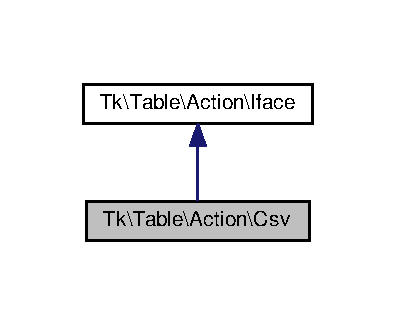
\includegraphics[width=190pt]{classTk_1_1Table_1_1Action_1_1Csv__inherit__graph}
\end{center}
\end{figure}
\subsection*{Public Member Functions}
\begin{DoxyCompactItemize}
\item 
\hyperlink{classTk_1_1Table_1_1Action_1_1Csv_a79bcb8e4e9eabd68d6f3ddee19e5baf1}{\+\_\+\+\_\+construct} (\$name= 'csv', \$checkbox\+Name= 'id')
\item 
\hyperlink{classTk_1_1Table_1_1Action_1_1Csv_a31f5863b31f521b484ac874f37c783d6}{execute} ()
\item 
\hyperlink{classTk_1_1Table_1_1Action_1_1Csv_a1bcda4d0684a52def0aa6917bd1b9292}{get\+Html} ()
\end{DoxyCompactItemize}
\subsection*{Protected Attributes}
\begin{DoxyCompactItemize}
\item 
\hypertarget{classTk_1_1Table_1_1Action_1_1Csv_ad1cc4240c977306d4c93244c85bb0233}{{\bfseries \$checkbox\+Name} = 'id'}\label{classTk_1_1Table_1_1Action_1_1Csv_ad1cc4240c977306d4c93244c85bb0233}

\end{DoxyCompactItemize}


\subsection{Detailed Description}
\begin{DoxyAuthor}{Author}
Michael Mifsud \href{mailto:info@tropotek.com}{\tt info@tropotek.\+com} \hyperlink{}{Copyright 2015 Michael Mifsud }
\end{DoxyAuthor}


\subsection{Constructor \& Destructor Documentation}
\hypertarget{classTk_1_1Table_1_1Action_1_1Csv_a79bcb8e4e9eabd68d6f3ddee19e5baf1}{\index{Tk\+::\+Table\+::\+Action\+::\+Csv@{Tk\+::\+Table\+::\+Action\+::\+Csv}!\+\_\+\+\_\+construct@{\+\_\+\+\_\+construct}}
\index{\+\_\+\+\_\+construct@{\+\_\+\+\_\+construct}!Tk\+::\+Table\+::\+Action\+::\+Csv@{Tk\+::\+Table\+::\+Action\+::\+Csv}}
\subsubsection[{\+\_\+\+\_\+construct}]{\setlength{\rightskip}{0pt plus 5cm}Tk\textbackslash{}\+Table\textbackslash{}\+Action\textbackslash{}\+Csv\+::\+\_\+\+\_\+construct (
\begin{DoxyParamCaption}
\item[{}]{\$name = {\ttfamily 'csv'}, }
\item[{}]{\$checkbox\+Name = {\ttfamily 'id'}}
\end{DoxyParamCaption}
)}}\label{classTk_1_1Table_1_1Action_1_1Csv_a79bcb8e4e9eabd68d6f3ddee19e5baf1}
Create


\begin{DoxyParams}[1]{Parameters}
string & {\em \$name} & \\
\hline
string & {\em \$checkbox\+Name} & \\
\hline
\end{DoxyParams}


\subsection{Member Function Documentation}
\hypertarget{classTk_1_1Table_1_1Action_1_1Csv_a31f5863b31f521b484ac874f37c783d6}{\index{Tk\+::\+Table\+::\+Action\+::\+Csv@{Tk\+::\+Table\+::\+Action\+::\+Csv}!execute@{execute}}
\index{execute@{execute}!Tk\+::\+Table\+::\+Action\+::\+Csv@{Tk\+::\+Table\+::\+Action\+::\+Csv}}
\subsubsection[{execute}]{\setlength{\rightskip}{0pt plus 5cm}Tk\textbackslash{}\+Table\textbackslash{}\+Action\textbackslash{}\+Csv\+::execute (
\begin{DoxyParamCaption}
{}
\end{DoxyParamCaption}
)}}\label{classTk_1_1Table_1_1Action_1_1Csv_a31f5863b31f521b484ac874f37c783d6}
\begin{DoxyReturn}{Returns}
mixed 
\end{DoxyReturn}
\hypertarget{classTk_1_1Table_1_1Action_1_1Csv_a1bcda4d0684a52def0aa6917bd1b9292}{\index{Tk\+::\+Table\+::\+Action\+::\+Csv@{Tk\+::\+Table\+::\+Action\+::\+Csv}!get\+Html@{get\+Html}}
\index{get\+Html@{get\+Html}!Tk\+::\+Table\+::\+Action\+::\+Csv@{Tk\+::\+Table\+::\+Action\+::\+Csv}}
\subsubsection[{get\+Html}]{\setlength{\rightskip}{0pt plus 5cm}Tk\textbackslash{}\+Table\textbackslash{}\+Action\textbackslash{}\+Csv\+::get\+Html (
\begin{DoxyParamCaption}
{}
\end{DoxyParamCaption}
)}}\label{classTk_1_1Table_1_1Action_1_1Csv_a1bcda4d0684a52def0aa6917bd1b9292}
\begin{DoxyReturn}{Returns}
string$\vert$ 
\end{DoxyReturn}


The documentation for this class was generated from the following file\+:\begin{DoxyCompactItemize}
\item 
vendor/ttek/tk-\/table/\+Tk/\+Table/\+Action/Csv.\+php\end{DoxyCompactItemize}

\hypertarget{classTk_1_1Form_1_1Renderer_1_1Dom_1_1Field_1_1Date}{\section{Tk\textbackslash{}Form\textbackslash{}Renderer\textbackslash{}Dom\textbackslash{}Field\textbackslash{}Date Class Reference}
\label{classTk_1_1Form_1_1Renderer_1_1Dom_1_1Field_1_1Date}\index{Tk\textbackslash{}\+Form\textbackslash{}\+Renderer\textbackslash{}\+Dom\textbackslash{}\+Field\textbackslash{}\+Date@{Tk\textbackslash{}\+Form\textbackslash{}\+Renderer\textbackslash{}\+Dom\textbackslash{}\+Field\textbackslash{}\+Date}}
}


Inheritance diagram for Tk\textbackslash{}Form\textbackslash{}Renderer\textbackslash{}Dom\textbackslash{}Field\textbackslash{}Date\+:\nopagebreak
\begin{figure}[H]
\begin{center}
\leavevmode
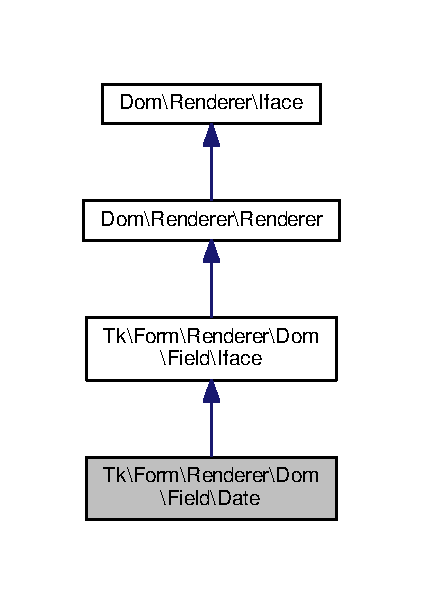
\includegraphics[width=203pt]{classTk_1_1Form_1_1Renderer_1_1Dom_1_1Field_1_1Date__inherit__graph}
\end{center}
\end{figure}
\subsection*{Public Member Functions}
\begin{DoxyCompactItemize}
\item 
\hyperlink{classTk_1_1Form_1_1Renderer_1_1Dom_1_1Field_1_1Date_aaa7073d65826e175d30157cafafe9b66}{\+\_\+\+\_\+construct} (\hyperlink{classTk_1_1Form_1_1Renderer_1_1Dom_1_1Field_1_1Iface}{Field\textbackslash{}\+Iface} \$field)
\item 
\hyperlink{classTk_1_1Form_1_1Renderer_1_1Dom_1_1Field_1_1Date_a5ce4951aefa90b53837ce13c9c911380}{\+\_\+\+\_\+make\+Template} ()
\end{DoxyCompactItemize}
\subsection*{Additional Inherited Members}


\subsection{Detailed Description}
Class \hyperlink{classTk_1_1Form_1_1Renderer_1_1Dom_1_1Field_1_1Date}{Date}

\begin{DoxyRefDesc}{Todo}
\item[\hyperlink{todo__todo000001}{Todo}]\+: get the date fromat from the Date\+Time field type object\end{DoxyRefDesc}


\begin{DoxyAuthor}{Author}
Michael Mifsud \href{mailto:info@tropotek.com}{\tt info@tropotek.\+com} \hyperlink{}{Copyright 2015 Michael Mifsud }
\end{DoxyAuthor}


\subsection{Constructor \& Destructor Documentation}
\hypertarget{classTk_1_1Form_1_1Renderer_1_1Dom_1_1Field_1_1Date_aaa7073d65826e175d30157cafafe9b66}{\index{Tk\+::\+Form\+::\+Renderer\+::\+Dom\+::\+Field\+::\+Date@{Tk\+::\+Form\+::\+Renderer\+::\+Dom\+::\+Field\+::\+Date}!\+\_\+\+\_\+construct@{\+\_\+\+\_\+construct}}
\index{\+\_\+\+\_\+construct@{\+\_\+\+\_\+construct}!Tk\+::\+Form\+::\+Renderer\+::\+Dom\+::\+Field\+::\+Date@{Tk\+::\+Form\+::\+Renderer\+::\+Dom\+::\+Field\+::\+Date}}
\subsubsection[{\+\_\+\+\_\+construct}]{\setlength{\rightskip}{0pt plus 5cm}Tk\textbackslash{}\+Form\textbackslash{}\+Renderer\textbackslash{}\+Dom\textbackslash{}\+Field\textbackslash{}\+Date\+::\+\_\+\+\_\+construct (
\begin{DoxyParamCaption}
\item[{{\bf Field\textbackslash{}\+Iface}}]{\$field}
\end{DoxyParamCaption}
)}}\label{classTk_1_1Form_1_1Renderer_1_1Dom_1_1Field_1_1Date_aaa7073d65826e175d30157cafafe9b66}
\+\_\+\+\_\+construct


\begin{DoxyParams}[1]{Parameters}
Field\textbackslash{}\+Iface & {\em \$field} & \\
\hline
\end{DoxyParams}


\subsection{Member Function Documentation}
\hypertarget{classTk_1_1Form_1_1Renderer_1_1Dom_1_1Field_1_1Date_a5ce4951aefa90b53837ce13c9c911380}{\index{Tk\+::\+Form\+::\+Renderer\+::\+Dom\+::\+Field\+::\+Date@{Tk\+::\+Form\+::\+Renderer\+::\+Dom\+::\+Field\+::\+Date}!\+\_\+\+\_\+make\+Template@{\+\_\+\+\_\+make\+Template}}
\index{\+\_\+\+\_\+make\+Template@{\+\_\+\+\_\+make\+Template}!Tk\+::\+Form\+::\+Renderer\+::\+Dom\+::\+Field\+::\+Date@{Tk\+::\+Form\+::\+Renderer\+::\+Dom\+::\+Field\+::\+Date}}
\subsubsection[{\+\_\+\+\_\+make\+Template}]{\setlength{\rightskip}{0pt plus 5cm}Tk\textbackslash{}\+Form\textbackslash{}\+Renderer\textbackslash{}\+Dom\textbackslash{}\+Field\textbackslash{}\+Date\+::\+\_\+\+\_\+make\+Template (
\begin{DoxyParamCaption}
{}
\end{DoxyParamCaption}
)}}\label{classTk_1_1Form_1_1Renderer_1_1Dom_1_1Field_1_1Date_a5ce4951aefa90b53837ce13c9c911380}
The default element template

Future H\+T\+M\+L5 date type elements\+: $<$input type=\char`\"{}month\char`\"{}$>$ $<$input type=\char`\"{}week\char`\"{}$>$ $<$input type=\char`\"{}time\char`\"{}$>$ $<$input type=\char`\"{}datetime\char`\"{}$>$ $<$input type=\char`\"{}datetime-\/local\char`\"{}$>$

\begin{DoxyReturn}{Returns}

\end{DoxyReturn}


The documentation for this class was generated from the following file\+:\begin{DoxyCompactItemize}
\item 
vendor/ttek/tk-\/form/\+Tk/\+Form/\+Renderer/\+Dom/\+Field/Date.\+php\end{DoxyCompactItemize}

\hypertarget{classTk_1_1Table_1_1Cell_1_1Date}{\section{Tk\textbackslash{}Table\textbackslash{}Cell\textbackslash{}Date Class Reference}
\label{classTk_1_1Table_1_1Cell_1_1Date}\index{Tk\textbackslash{}\+Table\textbackslash{}\+Cell\textbackslash{}\+Date@{Tk\textbackslash{}\+Table\textbackslash{}\+Cell\textbackslash{}\+Date}}
}


Inheritance diagram for Tk\textbackslash{}Table\textbackslash{}Cell\textbackslash{}Date\+:\nopagebreak
\begin{figure}[H]
\begin{center}
\leavevmode
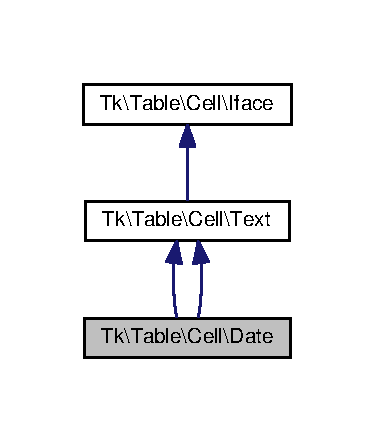
\includegraphics[width=180pt]{classTk_1_1Table_1_1Cell_1_1Date__inherit__graph}
\end{center}
\end{figure}
\subsection*{Public Member Functions}
\begin{DoxyCompactItemize}
\item 
\hyperlink{classTk_1_1Table_1_1Cell_1_1Date_a3187a53a6f025a9e04b8fca7d90ab97c}{set\+Format} (\$format)
\item 
\hyperlink{classTk_1_1Table_1_1Cell_1_1Date_afda49cc998bf4d98de6879a60359ab88}{get\+Property\+Value} (\$obj, \$property)
\item 
\hyperlink{classTk_1_1Table_1_1Cell_1_1Date_aebc9d2c9ccbddbf992139a3d163b65b2}{get\+Cell\+Html} (\$obj)
\end{DoxyCompactItemize}
\subsection*{Public Attributes}
\begin{DoxyCompactItemize}
\item 
\hypertarget{classTk_1_1Table_1_1Cell_1_1Date_a10db1c17bccbe75882eb265aa5453ada}{const {\bfseries F\+O\+R\+M\+A\+T\+\_\+\+R\+E\+L\+A\+T\+I\+V\+E} = 'relative'}\label{classTk_1_1Table_1_1Cell_1_1Date_a10db1c17bccbe75882eb265aa5453ada}

\end{DoxyCompactItemize}
\subsection*{Protected Attributes}
\begin{DoxyCompactItemize}
\item 
\hypertarget{classTk_1_1Table_1_1Cell_1_1Date_ab2a3e7c2766723925193b76859d34925}{{\bfseries \$format} = 'Y-\/m-\/d h\+:i\+:s'}\label{classTk_1_1Table_1_1Cell_1_1Date_ab2a3e7c2766723925193b76859d34925}

\end{DoxyCompactItemize}


\subsection{Detailed Description}
Class \hyperlink{classTk_1_1Table_1_1Cell_1_1Text}{Text}

\begin{DoxyAuthor}{Author}
Michael Mifsud \href{mailto:info@tropotek.com}{\tt info@tropotek.\+com} \hyperlink{}{Copyright 2015 Michael Mifsud }
\end{DoxyAuthor}


\subsection{Member Function Documentation}
\hypertarget{classTk_1_1Table_1_1Cell_1_1Date_aebc9d2c9ccbddbf992139a3d163b65b2}{\index{Tk\+::\+Table\+::\+Cell\+::\+Date@{Tk\+::\+Table\+::\+Cell\+::\+Date}!get\+Cell\+Html@{get\+Cell\+Html}}
\index{get\+Cell\+Html@{get\+Cell\+Html}!Tk\+::\+Table\+::\+Cell\+::\+Date@{Tk\+::\+Table\+::\+Cell\+::\+Date}}
\subsubsection[{get\+Cell\+Html}]{\setlength{\rightskip}{0pt plus 5cm}Tk\textbackslash{}\+Table\textbackslash{}\+Cell\textbackslash{}\+Date\+::get\+Cell\+Html (
\begin{DoxyParamCaption}
\item[{}]{\$obj}
\end{DoxyParamCaption}
)}}\label{classTk_1_1Table_1_1Cell_1_1Date_aebc9d2c9ccbddbf992139a3d163b65b2}

\begin{DoxyParams}[1]{Parameters}
mixed & {\em \$obj} & \\
\hline
\end{DoxyParams}
\begin{DoxyReturn}{Returns}
string 
\end{DoxyReturn}
\hypertarget{classTk_1_1Table_1_1Cell_1_1Date_afda49cc998bf4d98de6879a60359ab88}{\index{Tk\+::\+Table\+::\+Cell\+::\+Date@{Tk\+::\+Table\+::\+Cell\+::\+Date}!get\+Property\+Value@{get\+Property\+Value}}
\index{get\+Property\+Value@{get\+Property\+Value}!Tk\+::\+Table\+::\+Cell\+::\+Date@{Tk\+::\+Table\+::\+Cell\+::\+Date}}
\subsubsection[{get\+Property\+Value}]{\setlength{\rightskip}{0pt plus 5cm}Tk\textbackslash{}\+Table\textbackslash{}\+Cell\textbackslash{}\+Date\+::get\+Property\+Value (
\begin{DoxyParamCaption}
\item[{}]{\$obj, }
\item[{}]{\$property}
\end{DoxyParamCaption}
)}}\label{classTk_1_1Table_1_1Cell_1_1Date_afda49cc998bf4d98de6879a60359ab88}
Get the property value from the object using the supplied property name


\begin{DoxyParams}[1]{Parameters}
\textbackslash{}\+Date\+Time & {\em \$obj} & \\
\hline
string & {\em \$property} & \\
\hline
\end{DoxyParams}
\begin{DoxyReturn}{Returns}
string 
\end{DoxyReturn}
\hypertarget{classTk_1_1Table_1_1Cell_1_1Date_a3187a53a6f025a9e04b8fca7d90ab97c}{\index{Tk\+::\+Table\+::\+Cell\+::\+Date@{Tk\+::\+Table\+::\+Cell\+::\+Date}!set\+Format@{set\+Format}}
\index{set\+Format@{set\+Format}!Tk\+::\+Table\+::\+Cell\+::\+Date@{Tk\+::\+Table\+::\+Cell\+::\+Date}}
\subsubsection[{set\+Format}]{\setlength{\rightskip}{0pt plus 5cm}Tk\textbackslash{}\+Table\textbackslash{}\+Cell\textbackslash{}\+Date\+::set\+Format (
\begin{DoxyParamCaption}
\item[{}]{\$format}
\end{DoxyParamCaption}
)}}\label{classTk_1_1Table_1_1Cell_1_1Date_a3187a53a6f025a9e04b8fca7d90ab97c}
Change the format of the date


\begin{DoxyParams}{Parameters}
{\em \$format} & \\
\hline
\end{DoxyParams}
\begin{DoxyReturn}{Returns}
\$this 
\end{DoxyReturn}


The documentation for this class was generated from the following files\+:\begin{DoxyCompactItemize}
\item 
vendor/ttek/tk-\/table/\+Tk/\+Table/\+Cell/Date.\+php\item 
vendor/ttek/tk-\/table/\+Tk/\+Table/\+Cell/Email.\+php\end{DoxyCompactItemize}

\hypertarget{classTk_1_1Form_1_1Type_1_1DateTime}{\section{Tk\textbackslash{}Form\textbackslash{}Type\textbackslash{}Date\+Time Class Reference}
\label{classTk_1_1Form_1_1Type_1_1DateTime}\index{Tk\textbackslash{}\+Form\textbackslash{}\+Type\textbackslash{}\+Date\+Time@{Tk\textbackslash{}\+Form\textbackslash{}\+Type\textbackslash{}\+Date\+Time}}
}


Inheritance diagram for Tk\textbackslash{}Form\textbackslash{}Type\textbackslash{}Date\+Time\+:\nopagebreak
\begin{figure}[H]
\begin{center}
\leavevmode
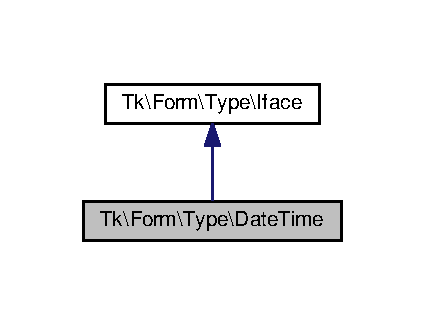
\includegraphics[width=204pt]{classTk_1_1Form_1_1Type_1_1DateTime__inherit__graph}
\end{center}
\end{figure}
\subsection*{Public Member Functions}
\begin{DoxyCompactItemize}
\item 
\hyperlink{classTk_1_1Form_1_1Type_1_1DateTime_a9e5a3c1d7a546b3cdf88096ef6f11b50}{to\+Type} (\$array)
\end{DoxyCompactItemize}
\subsection*{Additional Inherited Members}


\subsection{Detailed Description}
Class \hyperlink{classTk_1_1Form_1_1Type_1_1DateTime}{Date\+Time}

\begin{DoxyRefDesc}{Todo}
\item[\hyperlink{todo__todo000002}{Todo}]\+: Add a format parameter in the constructor so the date format can be specified\end{DoxyRefDesc}


\begin{DoxyAuthor}{Author}
Michael Mifsud \href{mailto:info@tropotek.com}{\tt info@tropotek.\+com} \hyperlink{}{Copyright 2015 Michael Mifsud }
\end{DoxyAuthor}


\subsection{Member Function Documentation}
\hypertarget{classTk_1_1Form_1_1Type_1_1DateTime_a9e5a3c1d7a546b3cdf88096ef6f11b50}{\index{Tk\+::\+Form\+::\+Type\+::\+Date\+Time@{Tk\+::\+Form\+::\+Type\+::\+Date\+Time}!to\+Type@{to\+Type}}
\index{to\+Type@{to\+Type}!Tk\+::\+Form\+::\+Type\+::\+Date\+Time@{Tk\+::\+Form\+::\+Type\+::\+Date\+Time}}
\subsubsection[{to\+Type}]{\setlength{\rightskip}{0pt plus 5cm}Tk\textbackslash{}\+Form\textbackslash{}\+Type\textbackslash{}\+Date\+Time\+::to\+Type (
\begin{DoxyParamCaption}
\item[{}]{\$array}
\end{DoxyParamCaption}
)}}\label{classTk_1_1Form_1_1Type_1_1DateTime_a9e5a3c1d7a546b3cdf88096ef6f11b50}
Convert the basic form submitted string field value into its correct complex type.


\begin{DoxyParams}[1]{Parameters}
array | \textbackslash{}std\+Class & {\em \$array} & \\
\hline
\end{DoxyParams}
\begin{DoxyReturn}{Returns}
mixed 
\end{DoxyReturn}


The documentation for this class was generated from the following file\+:\begin{DoxyCompactItemize}
\item 
vendor/ttek/tk-\/form/\+Tk/\+Form/\+Type/Date\+Time.\+php\end{DoxyCompactItemize}

\hypertarget{classDom_1_1Loader_1_1Adapter_1_1DefaultLoader}{\section{Dom\textbackslash{}Loader\textbackslash{}Adapter\textbackslash{}Default\+Loader Class Reference}
\label{classDom_1_1Loader_1_1Adapter_1_1DefaultLoader}\index{Dom\textbackslash{}\+Loader\textbackslash{}\+Adapter\textbackslash{}\+Default\+Loader@{Dom\textbackslash{}\+Loader\textbackslash{}\+Adapter\textbackslash{}\+Default\+Loader}}
}


Inheritance diagram for Dom\textbackslash{}Loader\textbackslash{}Adapter\textbackslash{}Default\+Loader\+:\nopagebreak
\begin{figure}[H]
\begin{center}
\leavevmode
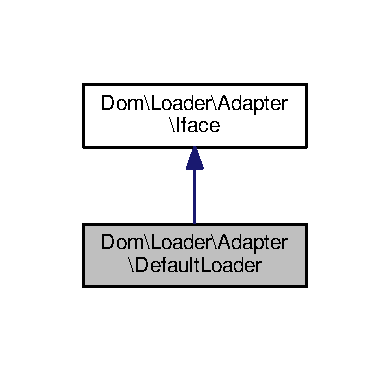
\includegraphics[width=187pt]{classDom_1_1Loader_1_1Adapter_1_1DefaultLoader__inherit__graph}
\end{center}
\end{figure}
\subsection*{Public Member Functions}
\begin{DoxyCompactItemize}
\item 
\hyperlink{classDom_1_1Loader_1_1Adapter_1_1DefaultLoader_af62cd152bf967d613f01d5a2385ca4ca}{load} (\$xhtml, \$class)
\item 
\hyperlink{classDom_1_1Loader_1_1Adapter_1_1DefaultLoader_aa04f96e1d4346aee79973cf2d7420181}{load\+File} (\$path, \$class)
\end{DoxyCompactItemize}
\subsection*{Additional Inherited Members}


\subsection{Detailed Description}
Default adapter for the loader object.

This should be run last after all other adapters have been tried

\begin{DoxyAuthor}{Author}
Michael Mifsud \href{mailto:info@tropotek.com}{\tt info@tropotek.\+com} \hyperlink{}{Copyright 2015 Michael Mifsud }
\end{DoxyAuthor}


\subsection{Member Function Documentation}
\hypertarget{classDom_1_1Loader_1_1Adapter_1_1DefaultLoader_af62cd152bf967d613f01d5a2385ca4ca}{\index{Dom\+::\+Loader\+::\+Adapter\+::\+Default\+Loader@{Dom\+::\+Loader\+::\+Adapter\+::\+Default\+Loader}!load@{load}}
\index{load@{load}!Dom\+::\+Loader\+::\+Adapter\+::\+Default\+Loader@{Dom\+::\+Loader\+::\+Adapter\+::\+Default\+Loader}}
\subsubsection[{load}]{\setlength{\rightskip}{0pt plus 5cm}Dom\textbackslash{}\+Loader\textbackslash{}\+Adapter\textbackslash{}\+Default\+Loader\+::load (
\begin{DoxyParamCaption}
\item[{}]{\$xhtml, }
\item[{}]{\$class}
\end{DoxyParamCaption}
)}}\label{classDom_1_1Loader_1_1Adapter_1_1DefaultLoader_af62cd152bf967d613f01d5a2385ca4ca}
Load an xml/xhtml strings


\begin{DoxyParams}{Parameters}
{\em \$xhtml} & \\
\hline
{\em \$class} & \\
\hline
\end{DoxyParams}
\begin{DoxyReturn}{Returns}
\hyperlink{classDom_1_1Template}{Template} 
\end{DoxyReturn}
\hypertarget{classDom_1_1Loader_1_1Adapter_1_1DefaultLoader_aa04f96e1d4346aee79973cf2d7420181}{\index{Dom\+::\+Loader\+::\+Adapter\+::\+Default\+Loader@{Dom\+::\+Loader\+::\+Adapter\+::\+Default\+Loader}!load\+File@{load\+File}}
\index{load\+File@{load\+File}!Dom\+::\+Loader\+::\+Adapter\+::\+Default\+Loader@{Dom\+::\+Loader\+::\+Adapter\+::\+Default\+Loader}}
\subsubsection[{load\+File}]{\setlength{\rightskip}{0pt plus 5cm}Dom\textbackslash{}\+Loader\textbackslash{}\+Adapter\textbackslash{}\+Default\+Loader\+::load\+File (
\begin{DoxyParamCaption}
\item[{}]{\$path, }
\item[{}]{\$class}
\end{DoxyParamCaption}
)}}\label{classDom_1_1Loader_1_1Adapter_1_1DefaultLoader_aa04f96e1d4346aee79973cf2d7420181}
Load an xml/xhtml file


\begin{DoxyParams}{Parameters}
{\em \$path} & \\
\hline
{\em \$class} & \\
\hline
\end{DoxyParams}
\begin{DoxyReturn}{Returns}
\hyperlink{classDom_1_1Template}{Template} 
\end{DoxyReturn}


The documentation for this class was generated from the following file\+:\begin{DoxyCompactItemize}
\item 
vendor/ttek/tk-\/domtemplate/\+Dom/\+Loader/\+Adapter/Default\+Loader.\+php\end{DoxyCompactItemize}

\hypertarget{classTk_1_1Table_1_1Action_1_1Delete}{\section{Tk\textbackslash{}Table\textbackslash{}Action\textbackslash{}Delete Class Reference}
\label{classTk_1_1Table_1_1Action_1_1Delete}\index{Tk\textbackslash{}\+Table\textbackslash{}\+Action\textbackslash{}\+Delete@{Tk\textbackslash{}\+Table\textbackslash{}\+Action\textbackslash{}\+Delete}}
}


Inheritance diagram for Tk\textbackslash{}Table\textbackslash{}Action\textbackslash{}Delete\+:\nopagebreak
\begin{figure}[H]
\begin{center}
\leavevmode
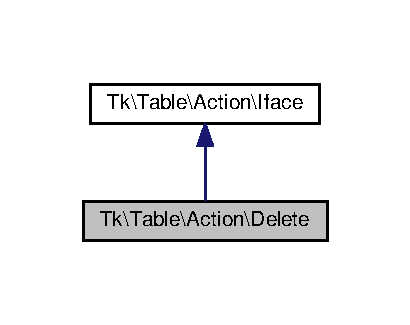
\includegraphics[width=197pt]{classTk_1_1Table_1_1Action_1_1Delete__inherit__graph}
\end{center}
\end{figure}
\subsection*{Public Member Functions}
\begin{DoxyCompactItemize}
\item 
\hyperlink{classTk_1_1Table_1_1Action_1_1Delete_ad377d0f8fcd9dcf04a4982ab9ab74c07}{\+\_\+\+\_\+construct} (\$name= 'delete', \$checkbox\+Name= 'id', \$icon= 'glyphicon glyphicon-\/remove')
\item 
\hyperlink{classTk_1_1Table_1_1Action_1_1Delete_a72e574c6ae07ae2f7441f5273b2420c2}{get\+Html} ()
\end{DoxyCompactItemize}
\subsection*{Protected Attributes}
\begin{DoxyCompactItemize}
\item 
\hypertarget{classTk_1_1Table_1_1Action_1_1Delete_a3cd8c0ecf53f518caf596616d5080334}{{\bfseries \$icon} = ''}\label{classTk_1_1Table_1_1Action_1_1Delete_a3cd8c0ecf53f518caf596616d5080334}

\item 
\hypertarget{classTk_1_1Table_1_1Action_1_1Delete_a956c5bd1dfb444359beee796530e4ce9}{{\bfseries \$checkbox\+Name} = 'id'}\label{classTk_1_1Table_1_1Action_1_1Delete_a956c5bd1dfb444359beee796530e4ce9}

\end{DoxyCompactItemize}


\subsection{Detailed Description}
\begin{DoxyAuthor}{Author}
Michael Mifsud \href{mailto:info@tropotek.com}{\tt info@tropotek.\+com} \hyperlink{}{Copyright 2015 Michael Mifsud }
\end{DoxyAuthor}


\subsection{Constructor \& Destructor Documentation}
\hypertarget{classTk_1_1Table_1_1Action_1_1Delete_ad377d0f8fcd9dcf04a4982ab9ab74c07}{\index{Tk\+::\+Table\+::\+Action\+::\+Delete@{Tk\+::\+Table\+::\+Action\+::\+Delete}!\+\_\+\+\_\+construct@{\+\_\+\+\_\+construct}}
\index{\+\_\+\+\_\+construct@{\+\_\+\+\_\+construct}!Tk\+::\+Table\+::\+Action\+::\+Delete@{Tk\+::\+Table\+::\+Action\+::\+Delete}}
\subsubsection[{\+\_\+\+\_\+construct}]{\setlength{\rightskip}{0pt plus 5cm}Tk\textbackslash{}\+Table\textbackslash{}\+Action\textbackslash{}\+Delete\+::\+\_\+\+\_\+construct (
\begin{DoxyParamCaption}
\item[{}]{\$name = {\ttfamily 'delete'}, }
\item[{}]{\$checkbox\+Name = {\ttfamily 'id'}, }
\item[{}]{\$icon = {\ttfamily 'glyphicon~glyphicon-\/remove'}}
\end{DoxyParamCaption}
)}}\label{classTk_1_1Table_1_1Action_1_1Delete_ad377d0f8fcd9dcf04a4982ab9ab74c07}
Create


\begin{DoxyParams}[1]{Parameters}
string & {\em \$name} & \\
\hline
string & {\em \$checkbox\+Name} & The checkbox name to get the selected id's from \\
\hline
string & {\em \$icon} & \\
\hline
\end{DoxyParams}


\subsection{Member Function Documentation}
\hypertarget{classTk_1_1Table_1_1Action_1_1Delete_a72e574c6ae07ae2f7441f5273b2420c2}{\index{Tk\+::\+Table\+::\+Action\+::\+Delete@{Tk\+::\+Table\+::\+Action\+::\+Delete}!get\+Html@{get\+Html}}
\index{get\+Html@{get\+Html}!Tk\+::\+Table\+::\+Action\+::\+Delete@{Tk\+::\+Table\+::\+Action\+::\+Delete}}
\subsubsection[{get\+Html}]{\setlength{\rightskip}{0pt plus 5cm}Tk\textbackslash{}\+Table\textbackslash{}\+Action\textbackslash{}\+Delete\+::get\+Html (
\begin{DoxyParamCaption}
{}
\end{DoxyParamCaption}
)}}\label{classTk_1_1Table_1_1Action_1_1Delete_a72e574c6ae07ae2f7441f5273b2420c2}
\begin{DoxyReturn}{Returns}
string$\vert$ 
\end{DoxyReturn}


The documentation for this class was generated from the following file\+:\begin{DoxyCompactItemize}
\item 
vendor/ttek/tk-\/table/\+Tk/\+Table/\+Action/Delete.\+php\end{DoxyCompactItemize}

\hypertarget{classDom_1_1Form_1_1Element}{\section{Dom\textbackslash{}Form\textbackslash{}Element Class Reference}
\label{classDom_1_1Form_1_1Element}\index{Dom\textbackslash{}\+Form\textbackslash{}\+Element@{Dom\textbackslash{}\+Form\textbackslash{}\+Element}}
}


Inheritance diagram for Dom\textbackslash{}Form\textbackslash{}Element\+:\nopagebreak
\begin{figure}[H]
\begin{center}
\leavevmode
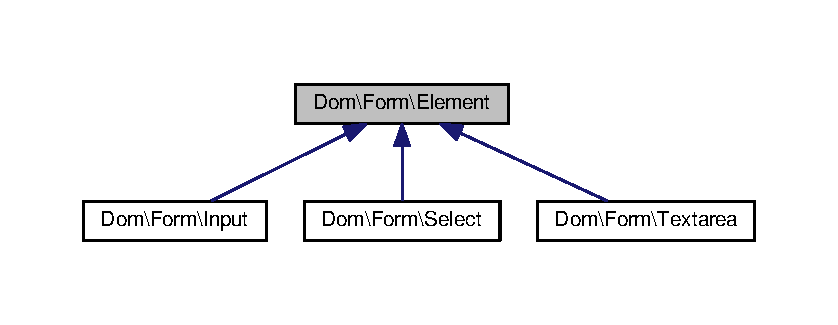
\includegraphics[width=350pt]{classDom_1_1Form_1_1Element__inherit__graph}
\end{center}
\end{figure}
\subsection*{Public Member Functions}
\begin{DoxyCompactItemize}
\item 
\hyperlink{classDom_1_1Form_1_1Element_a6ce880f508b05dd51b3da8f3e937ddf3}{\+\_\+\+\_\+construct} (\$element, \$form=null)
\item 
\hyperlink{classDom_1_1Form_1_1Element_ad6d9a61adec54cd4a0bc69b3438e8966}{set\+Name} (\$name)
\item 
\hyperlink{classDom_1_1Form_1_1Element_a73197b37d60104c2e35175b640d8c613}{get\+Name} ()
\item 
\hyperlink{classDom_1_1Form_1_1Element_a8ba319f18889a8629310065e974fc5cf}{get\+Node} ()
\item 
\hyperlink{classDom_1_1Form_1_1Element_aaa324956a3c1cc1c761018e2c7059b3b}{get\+Form} ()
\item 
\hyperlink{classDom_1_1Form_1_1Element_a5289f3b8137d9a6087ee7928bfcdcb13}{get\+Template} ()
\item 
\hyperlink{classDom_1_1Form_1_1Element_a9300ff63136238f244b2958b26b15543}{set\+Value} (\$value)
\item 
\hyperlink{classDom_1_1Form_1_1Element_a4dd060542b12b221c271be189a980536}{get\+Value} ()
\item 
\hyperlink{classDom_1_1Form_1_1Element_a63a05da078033cbfc7611b94107846c9}{get\+Type} ()
\item 
\hyperlink{classDom_1_1Form_1_1Element_a076eec1fb3cb9c6de75b8a542c3f0dcf}{disable} ()
\item 
\hyperlink{classDom_1_1Form_1_1Element_af99cd3a7e84f213b1e13f1dae4cfc1ed}{is\+Disabled} ()
\item 
\hyperlink{classDom_1_1Form_1_1Element_a514767ace45bc92f87b3927f3e4c7b26}{set\+Attribute} (\$name, \$value)
\item 
\hyperlink{classDom_1_1Form_1_1Element_ab9324099548b3f7d8e01ca4b78a7bf64}{get\+Attribute} (\$name)
\end{DoxyCompactItemize}
\subsection*{Protected Attributes}
\begin{DoxyCompactItemize}
\item 
\hypertarget{classDom_1_1Form_1_1Element_acc47d5447322fab467bfa067f5c70c2f}{{\bfseries \$element} = null}\label{classDom_1_1Form_1_1Element_acc47d5447322fab467bfa067f5c70c2f}

\item 
\hypertarget{classDom_1_1Form_1_1Element_ab3fca493114eb9e8de9b2e926451bb63}{{\bfseries \$form} = null}\label{classDom_1_1Form_1_1Element_ab3fca493114eb9e8de9b2e926451bb63}

\end{DoxyCompactItemize}


\subsection{Detailed Description}
All form elements must use this class/interface.

\begin{DoxyAuthor}{Author}
Michael Mifsud 

Darryl Ross \hyperlink{}{Copyright 2007 }
\end{DoxyAuthor}


\subsection{Constructor \& Destructor Documentation}
\hypertarget{classDom_1_1Form_1_1Element_a6ce880f508b05dd51b3da8f3e937ddf3}{\index{Dom\+::\+Form\+::\+Element@{Dom\+::\+Form\+::\+Element}!\+\_\+\+\_\+construct@{\+\_\+\+\_\+construct}}
\index{\+\_\+\+\_\+construct@{\+\_\+\+\_\+construct}!Dom\+::\+Form\+::\+Element@{Dom\+::\+Form\+::\+Element}}
\subsubsection[{\+\_\+\+\_\+construct}]{\setlength{\rightskip}{0pt plus 5cm}Dom\textbackslash{}\+Form\textbackslash{}\+Element\+::\+\_\+\+\_\+construct (
\begin{DoxyParamCaption}
\item[{}]{\$element, }
\item[{}]{\$form = {\ttfamily null}}
\end{DoxyParamCaption}
)}}\label{classDom_1_1Form_1_1Element_a6ce880f508b05dd51b3da8f3e937ddf3}
\+\_\+\+\_\+construct


\begin{DoxyParams}[1]{Parameters}
\textbackslash{}\+D\+O\+M\+Element & {\em \$element} & \\
\hline
\hyperlink{classDom_1_1Form}{Form} & {\em \$form} & \\
\hline
\end{DoxyParams}


\subsection{Member Function Documentation}
\hypertarget{classDom_1_1Form_1_1Element_a076eec1fb3cb9c6de75b8a542c3f0dcf}{\index{Dom\+::\+Form\+::\+Element@{Dom\+::\+Form\+::\+Element}!disable@{disable}}
\index{disable@{disable}!Dom\+::\+Form\+::\+Element@{Dom\+::\+Form\+::\+Element}}
\subsubsection[{disable}]{\setlength{\rightskip}{0pt plus 5cm}Dom\textbackslash{}\+Form\textbackslash{}\+Element\+::disable (
\begin{DoxyParamCaption}
{}
\end{DoxyParamCaption}
)}}\label{classDom_1_1Form_1_1Element_a076eec1fb3cb9c6de75b8a542c3f0dcf}
Disable this element, adds a disable attribute to the node

\begin{DoxyReturn}{Returns}
\$this 
\end{DoxyReturn}
\hypertarget{classDom_1_1Form_1_1Element_ab9324099548b3f7d8e01ca4b78a7bf64}{\index{Dom\+::\+Form\+::\+Element@{Dom\+::\+Form\+::\+Element}!get\+Attribute@{get\+Attribute}}
\index{get\+Attribute@{get\+Attribute}!Dom\+::\+Form\+::\+Element@{Dom\+::\+Form\+::\+Element}}
\subsubsection[{get\+Attribute}]{\setlength{\rightskip}{0pt plus 5cm}Dom\textbackslash{}\+Form\textbackslash{}\+Element\+::get\+Attribute (
\begin{DoxyParamCaption}
\item[{}]{\$name}
\end{DoxyParamCaption}
)}}\label{classDom_1_1Form_1_1Element_ab9324099548b3f7d8e01ca4b78a7bf64}
Set the name of this element


\begin{DoxyParams}[1]{Parameters}
string & {\em \$name} & \\
\hline
\end{DoxyParams}
\begin{DoxyReturn}{Returns}
string 
\end{DoxyReturn}
\hypertarget{classDom_1_1Form_1_1Element_aaa324956a3c1cc1c761018e2c7059b3b}{\index{Dom\+::\+Form\+::\+Element@{Dom\+::\+Form\+::\+Element}!get\+Form@{get\+Form}}
\index{get\+Form@{get\+Form}!Dom\+::\+Form\+::\+Element@{Dom\+::\+Form\+::\+Element}}
\subsubsection[{get\+Form}]{\setlength{\rightskip}{0pt plus 5cm}Dom\textbackslash{}\+Form\textbackslash{}\+Element\+::get\+Form (
\begin{DoxyParamCaption}
{}
\end{DoxyParamCaption}
)}}\label{classDom_1_1Form_1_1Element_aaa324956a3c1cc1c761018e2c7059b3b}
Get the parent D\+O\+M form object

\begin{DoxyReturn}{Returns}
\hyperlink{classDom_1_1Form}{Form} 
\end{DoxyReturn}
\hypertarget{classDom_1_1Form_1_1Element_a73197b37d60104c2e35175b640d8c613}{\index{Dom\+::\+Form\+::\+Element@{Dom\+::\+Form\+::\+Element}!get\+Name@{get\+Name}}
\index{get\+Name@{get\+Name}!Dom\+::\+Form\+::\+Element@{Dom\+::\+Form\+::\+Element}}
\subsubsection[{get\+Name}]{\setlength{\rightskip}{0pt plus 5cm}Dom\textbackslash{}\+Form\textbackslash{}\+Element\+::get\+Name (
\begin{DoxyParamCaption}
{}
\end{DoxyParamCaption}
)}}\label{classDom_1_1Form_1_1Element_a73197b37d60104c2e35175b640d8c613}
Get the name of this element

\begin{DoxyReturn}{Returns}
string The name of this element. 
\end{DoxyReturn}
\hypertarget{classDom_1_1Form_1_1Element_a8ba319f18889a8629310065e974fc5cf}{\index{Dom\+::\+Form\+::\+Element@{Dom\+::\+Form\+::\+Element}!get\+Node@{get\+Node}}
\index{get\+Node@{get\+Node}!Dom\+::\+Form\+::\+Element@{Dom\+::\+Form\+::\+Element}}
\subsubsection[{get\+Node}]{\setlength{\rightskip}{0pt plus 5cm}Dom\textbackslash{}\+Form\textbackslash{}\+Element\+::get\+Node (
\begin{DoxyParamCaption}
{}
\end{DoxyParamCaption}
)}}\label{classDom_1_1Form_1_1Element_a8ba319f18889a8629310065e974fc5cf}
Get the  node for this form element

\begin{DoxyReturn}{Returns}

\end{DoxyReturn}
\hypertarget{classDom_1_1Form_1_1Element_a5289f3b8137d9a6087ee7928bfcdcb13}{\index{Dom\+::\+Form\+::\+Element@{Dom\+::\+Form\+::\+Element}!get\+Template@{get\+Template}}
\index{get\+Template@{get\+Template}!Dom\+::\+Form\+::\+Element@{Dom\+::\+Form\+::\+Element}}
\subsubsection[{get\+Template}]{\setlength{\rightskip}{0pt plus 5cm}Dom\textbackslash{}\+Form\textbackslash{}\+Element\+::get\+Template (
\begin{DoxyParamCaption}
{}
\end{DoxyParamCaption}
)}}\label{classDom_1_1Form_1_1Element_a5289f3b8137d9a6087ee7928bfcdcb13}
Get the Type's \hyperlink{classDom_1_1Template}{Template}

\begin{DoxyReturn}{Returns}
\hyperlink{classDom_1_1Template}{Template} 
\end{DoxyReturn}
\hypertarget{classDom_1_1Form_1_1Element_a63a05da078033cbfc7611b94107846c9}{\index{Dom\+::\+Form\+::\+Element@{Dom\+::\+Form\+::\+Element}!get\+Type@{get\+Type}}
\index{get\+Type@{get\+Type}!Dom\+::\+Form\+::\+Element@{Dom\+::\+Form\+::\+Element}}
\subsubsection[{get\+Type}]{\setlength{\rightskip}{0pt plus 5cm}Dom\textbackslash{}\+Form\textbackslash{}\+Element\+::get\+Type (
\begin{DoxyParamCaption}
{}
\end{DoxyParamCaption}
)}}\label{classDom_1_1Form_1_1Element_a63a05da078033cbfc7611b94107846c9}
Return the form element type attribute

\begin{DoxyReturn}{Returns}
string 
\end{DoxyReturn}
\hypertarget{classDom_1_1Form_1_1Element_a4dd060542b12b221c271be189a980536}{\index{Dom\+::\+Form\+::\+Element@{Dom\+::\+Form\+::\+Element}!get\+Value@{get\+Value}}
\index{get\+Value@{get\+Value}!Dom\+::\+Form\+::\+Element@{Dom\+::\+Form\+::\+Element}}
\subsubsection[{get\+Value}]{\setlength{\rightskip}{0pt plus 5cm}Dom\textbackslash{}\+Form\textbackslash{}\+Element\+::get\+Value (
\begin{DoxyParamCaption}
{}
\end{DoxyParamCaption}
)\hspace{0.3cm}{\ttfamily [abstract]}}}\label{classDom_1_1Form_1_1Element_a4dd060542b12b221c271be189a980536}
Return the value of the element, or the selected value.

\begin{DoxyReturn}{Returns}
string$\vert$array A string or an array of strings for multiple select elements 
\end{DoxyReturn}
\hypertarget{classDom_1_1Form_1_1Element_af99cd3a7e84f213b1e13f1dae4cfc1ed}{\index{Dom\+::\+Form\+::\+Element@{Dom\+::\+Form\+::\+Element}!is\+Disabled@{is\+Disabled}}
\index{is\+Disabled@{is\+Disabled}!Dom\+::\+Form\+::\+Element@{Dom\+::\+Form\+::\+Element}}
\subsubsection[{is\+Disabled}]{\setlength{\rightskip}{0pt plus 5cm}Dom\textbackslash{}\+Form\textbackslash{}\+Element\+::is\+Disabled (
\begin{DoxyParamCaption}
{}
\end{DoxyParamCaption}
)}}\label{classDom_1_1Form_1_1Element_af99cd3a7e84f213b1e13f1dae4cfc1ed}
get the disabled state of this node

\begin{DoxyReturn}{Returns}
bool 
\end{DoxyReturn}
\hypertarget{classDom_1_1Form_1_1Element_a514767ace45bc92f87b3927f3e4c7b26}{\index{Dom\+::\+Form\+::\+Element@{Dom\+::\+Form\+::\+Element}!set\+Attribute@{set\+Attribute}}
\index{set\+Attribute@{set\+Attribute}!Dom\+::\+Form\+::\+Element@{Dom\+::\+Form\+::\+Element}}
\subsubsection[{set\+Attribute}]{\setlength{\rightskip}{0pt plus 5cm}Dom\textbackslash{}\+Form\textbackslash{}\+Element\+::set\+Attribute (
\begin{DoxyParamCaption}
\item[{}]{\$name, }
\item[{}]{\$value}
\end{DoxyParamCaption}
)}}\label{classDom_1_1Form_1_1Element_a514767ace45bc92f87b3927f3e4c7b26}
Set the attribute name and value


\begin{DoxyParams}[1]{Parameters}
string & {\em \$name} & \\
\hline
string & {\em \$value} & \\
\hline
\end{DoxyParams}
\begin{DoxyReturn}{Returns}
\$this 
\end{DoxyReturn}
\hypertarget{classDom_1_1Form_1_1Element_ad6d9a61adec54cd4a0bc69b3438e8966}{\index{Dom\+::\+Form\+::\+Element@{Dom\+::\+Form\+::\+Element}!set\+Name@{set\+Name}}
\index{set\+Name@{set\+Name}!Dom\+::\+Form\+::\+Element@{Dom\+::\+Form\+::\+Element}}
\subsubsection[{set\+Name}]{\setlength{\rightskip}{0pt plus 5cm}Dom\textbackslash{}\+Form\textbackslash{}\+Element\+::set\+Name (
\begin{DoxyParamCaption}
\item[{}]{\$name}
\end{DoxyParamCaption}
)}}\label{classDom_1_1Form_1_1Element_ad6d9a61adec54cd4a0bc69b3438e8966}
Set the name of this element


\begin{DoxyParams}[1]{Parameters}
string & {\em \$name} & \\
\hline
\end{DoxyParams}
\begin{DoxyReturn}{Returns}
\$this 
\end{DoxyReturn}
\hypertarget{classDom_1_1Form_1_1Element_a9300ff63136238f244b2958b26b15543}{\index{Dom\+::\+Form\+::\+Element@{Dom\+::\+Form\+::\+Element}!set\+Value@{set\+Value}}
\index{set\+Value@{set\+Value}!Dom\+::\+Form\+::\+Element@{Dom\+::\+Form\+::\+Element}}
\subsubsection[{set\+Value}]{\setlength{\rightskip}{0pt plus 5cm}Dom\textbackslash{}\+Form\textbackslash{}\+Element\+::set\+Value (
\begin{DoxyParamCaption}
\item[{}]{\$value}
\end{DoxyParamCaption}
)\hspace{0.3cm}{\ttfamily [abstract]}}}\label{classDom_1_1Form_1_1Element_a9300ff63136238f244b2958b26b15543}
Set the value of a form element.

Set value behaves different for different elements\+: o input =$>$ This is the element value attribute o checkbox/radio =$>$ The value to check/select o select =$>$ The value of the option to be selected o textarea =$>$ the content of the textarea


\begin{DoxyParams}[1]{Parameters}
string & {\em \$value} & \\
\hline
\end{DoxyParams}
\begin{DoxyReturn}{Returns}
\hyperlink{classDom_1_1Form_1_1Element}{Element} 
\end{DoxyReturn}


The documentation for this class was generated from the following file\+:\begin{DoxyCompactItemize}
\item 
vendor/ttek/tk-\/domtemplate/\+Dom/\+Form/Element.\+php\end{DoxyCompactItemize}

\hypertarget{classTk_1_1Form_1_1Element}{\section{Tk\textbackslash{}Form\textbackslash{}Element Class Reference}
\label{classTk_1_1Form_1_1Element}\index{Tk\textbackslash{}\+Form\textbackslash{}\+Element@{Tk\textbackslash{}\+Form\textbackslash{}\+Element}}
}


Inheritance diagram for Tk\textbackslash{}Form\textbackslash{}Element\+:\nopagebreak
\begin{figure}[H]
\begin{center}
\leavevmode
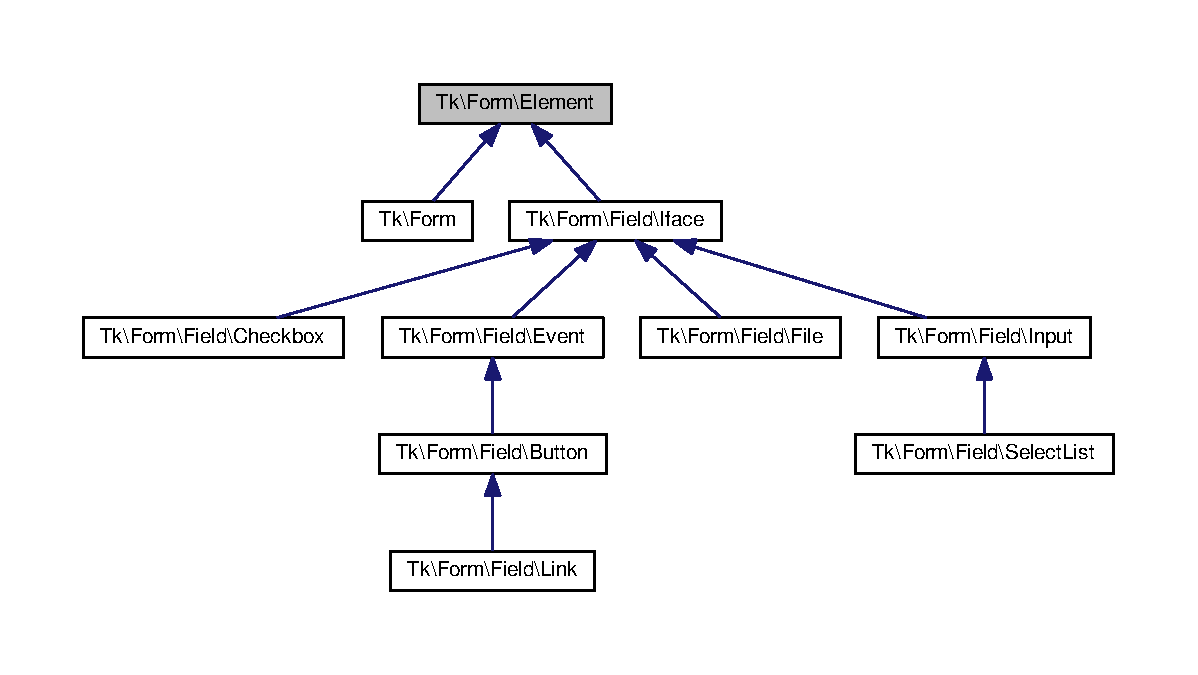
\includegraphics[width=350pt]{classTk_1_1Form_1_1Element__inherit__graph}
\end{center}
\end{figure}
\subsection*{Public Member Functions}
\begin{DoxyCompactItemize}
\item 
\hyperlink{classTk_1_1Form_1_1Element_ab2d444b43ec4898f0e7c3a820166361d}{get\+Name} ()
\item 
\hyperlink{classTk_1_1Form_1_1Element_a3be96916f13d347b9302b617ab70433c}{set\+Name} (\$name)
\item 
\hyperlink{classTk_1_1Form_1_1Element_a21676e35649e65aa1b25ac9650574791}{set\+Form} (\hyperlink{classTk_1_1Form}{Form} \$form)
\item 
\hyperlink{classTk_1_1Form_1_1Element_aebd859aa21a08ff2c853192d001ae854}{get\+Form} ()
\item 
\hyperlink{classTk_1_1Form_1_1Element_a44f96cdf51bb9fb1d0669ec1e5e3d391}{add\+Error} (\$msg)
\item 
\hyperlink{classTk_1_1Form_1_1Element_a28df7771e8ea01ab0d22155bf6e2d3f3}{get\+Errors} ()
\item 
\hyperlink{classTk_1_1Form_1_1Element_acc67fc16d36fdbb12112ea9635bef8d1}{set\+Errors} (\$errors=array())
\item 
\hyperlink{classTk_1_1Form_1_1Element_a0a8bca514435d24b95ca130a7d60d620}{has\+Errors} ()
\item 
\hyperlink{classTk_1_1Form_1_1Element_ad6daa5550f7be509ebd18e76c5365835}{set\+Attr} (\$attr\+Name, \$value)
\item 
\hyperlink{classTk_1_1Form_1_1Element_a51146497c5762879c4cdcb91ce0f3f9e}{get\+Attr} (\$attr\+Name)
\item 
\hyperlink{classTk_1_1Form_1_1Element_afe86ad6d478822dc54d6b0236364fe8a}{remove\+Attr} (\$attr\+Name)
\item 
\hyperlink{classTk_1_1Form_1_1Element_a0500123e165f8ea1d2088182f06d5593}{get\+Attr\+List} ()
\item 
\hyperlink{classTk_1_1Form_1_1Element_afcb2c07dc89c8c09bde82dd47fae2229}{set\+Attr\+List} (\$array=array())
\item 
\hyperlink{classTk_1_1Form_1_1Element_a68c5472ae89051f4ed159085949cd244}{add\+Css} (\$class\+Name)
\item 
\hyperlink{classTk_1_1Form_1_1Element_ac966da5b6d3e94e26fb611987de83483}{remove\+Css} (\$class\+Name)
\item 
\hyperlink{classTk_1_1Form_1_1Element_a1414fbd5a4cc6a12c7af1bf53e6720c5}{set\+Css\+List} (\$array=array())
\item 
\hyperlink{classTk_1_1Form_1_1Element_aefb70f35a6c60faf1c33e6df2b4ffe53}{get\+Css\+List} ()
\end{DoxyCompactItemize}
\subsection*{Protected Attributes}
\begin{DoxyCompactItemize}
\item 
\hypertarget{classTk_1_1Form_1_1Element_a37309d004ffc64ab80e7d6a64615e17b}{{\bfseries \$name} = ''}\label{classTk_1_1Form_1_1Element_a37309d004ffc64ab80e7d6a64615e17b}

\item 
\hypertarget{classTk_1_1Form_1_1Element_a45d840bb00ca5dced137e307f63d837e}{{\bfseries \$form} = null}\label{classTk_1_1Form_1_1Element_a45d840bb00ca5dced137e307f63d837e}

\item 
\hypertarget{classTk_1_1Form_1_1Element_a1eac3769c129c29272b15ac41cd97963}{{\bfseries \$errors} = array()}\label{classTk_1_1Form_1_1Element_a1eac3769c129c29272b15ac41cd97963}

\item 
\hypertarget{classTk_1_1Form_1_1Element_a8bda89f1632f18e2c20a9236b7a6ae60}{{\bfseries \$attr\+List} = array()}\label{classTk_1_1Form_1_1Element_a8bda89f1632f18e2c20a9236b7a6ae60}

\item 
\hypertarget{classTk_1_1Form_1_1Element_a3095696a8864703905a367055ac93c66}{{\bfseries \$css\+List} = array()}\label{classTk_1_1Form_1_1Element_a3095696a8864703905a367055ac93c66}

\end{DoxyCompactItemize}


\subsection{Detailed Description}
Interface \hyperlink{classTk_1_1Form_1_1Element}{Element}

\begin{DoxyAuthor}{Author}
Michael Mifsud \href{mailto:info@tropotek.com}{\tt info@tropotek.\+com} \hyperlink{}{Copyright 2015 Michael Mifsud }
\end{DoxyAuthor}


\subsection{Member Function Documentation}
\hypertarget{classTk_1_1Form_1_1Element_a68c5472ae89051f4ed159085949cd244}{\index{Tk\+::\+Form\+::\+Element@{Tk\+::\+Form\+::\+Element}!add\+Css@{add\+Css}}
\index{add\+Css@{add\+Css}!Tk\+::\+Form\+::\+Element@{Tk\+::\+Form\+::\+Element}}
\subsubsection[{add\+Css}]{\setlength{\rightskip}{0pt plus 5cm}Tk\textbackslash{}\+Form\textbackslash{}\+Element\+::add\+Css (
\begin{DoxyParamCaption}
\item[{}]{\$class\+Name}
\end{DoxyParamCaption}
)}}\label{classTk_1_1Form_1_1Element_a68c5472ae89051f4ed159085949cd244}
Add a C\+S\+S Class name to the node


\begin{DoxyParams}[1]{Parameters}
string & {\em \$class\+Name} & \\
\hline
\end{DoxyParams}
\begin{DoxyReturn}{Returns}
\$this 
\end{DoxyReturn}
\hypertarget{classTk_1_1Form_1_1Element_a44f96cdf51bb9fb1d0669ec1e5e3d391}{\index{Tk\+::\+Form\+::\+Element@{Tk\+::\+Form\+::\+Element}!add\+Error@{add\+Error}}
\index{add\+Error@{add\+Error}!Tk\+::\+Form\+::\+Element@{Tk\+::\+Form\+::\+Element}}
\subsubsection[{add\+Error}]{\setlength{\rightskip}{0pt plus 5cm}Tk\textbackslash{}\+Form\textbackslash{}\+Element\+::add\+Error (
\begin{DoxyParamCaption}
\item[{}]{\$msg}
\end{DoxyParamCaption}
)}}\label{classTk_1_1Form_1_1Element_a44f96cdf51bb9fb1d0669ec1e5e3d391}
Add an error message html to the element


\begin{DoxyParams}[1]{Parameters}
string | array & {\em \$msg} & \\
\hline
\end{DoxyParams}
\begin{DoxyReturn}{Returns}
\$this 
\end{DoxyReturn}
\hypertarget{classTk_1_1Form_1_1Element_a51146497c5762879c4cdcb91ce0f3f9e}{\index{Tk\+::\+Form\+::\+Element@{Tk\+::\+Form\+::\+Element}!get\+Attr@{get\+Attr}}
\index{get\+Attr@{get\+Attr}!Tk\+::\+Form\+::\+Element@{Tk\+::\+Form\+::\+Element}}
\subsubsection[{get\+Attr}]{\setlength{\rightskip}{0pt plus 5cm}Tk\textbackslash{}\+Form\textbackslash{}\+Element\+::get\+Attr (
\begin{DoxyParamCaption}
\item[{}]{\$attr\+Name}
\end{DoxyParamCaption}
)}}\label{classTk_1_1Form_1_1Element_a51146497c5762879c4cdcb91ce0f3f9e}
Get an attribute from this node N\+O\+T\+E\+: You can only retrieve attributes that have been set via \hyperlink{classTk_1_1Form_1_1Element_ad6daa5550f7be509ebd18e76c5365835}{set\+Attr()}


\begin{DoxyParams}[1]{Parameters}
string & {\em \$attr\+Name} & \\
\hline
\end{DoxyParams}
\begin{DoxyReturn}{Returns}
string$\vert$null 
\end{DoxyReturn}
\hypertarget{classTk_1_1Form_1_1Element_a0500123e165f8ea1d2088182f06d5593}{\index{Tk\+::\+Form\+::\+Element@{Tk\+::\+Form\+::\+Element}!get\+Attr\+List@{get\+Attr\+List}}
\index{get\+Attr\+List@{get\+Attr\+List}!Tk\+::\+Form\+::\+Element@{Tk\+::\+Form\+::\+Element}}
\subsubsection[{get\+Attr\+List}]{\setlength{\rightskip}{0pt plus 5cm}Tk\textbackslash{}\+Form\textbackslash{}\+Element\+::get\+Attr\+List (
\begin{DoxyParamCaption}
{}
\end{DoxyParamCaption}
)}}\label{classTk_1_1Form_1_1Element_a0500123e165f8ea1d2088182f06d5593}
Get the attribute list

\begin{DoxyReturn}{Returns}
array 
\end{DoxyReturn}
\hypertarget{classTk_1_1Form_1_1Element_aefb70f35a6c60faf1c33e6df2b4ffe53}{\index{Tk\+::\+Form\+::\+Element@{Tk\+::\+Form\+::\+Element}!get\+Css\+List@{get\+Css\+List}}
\index{get\+Css\+List@{get\+Css\+List}!Tk\+::\+Form\+::\+Element@{Tk\+::\+Form\+::\+Element}}
\subsubsection[{get\+Css\+List}]{\setlength{\rightskip}{0pt plus 5cm}Tk\textbackslash{}\+Form\textbackslash{}\+Element\+::get\+Css\+List (
\begin{DoxyParamCaption}
{}
\end{DoxyParamCaption}
)}}\label{classTk_1_1Form_1_1Element_aefb70f35a6c60faf1c33e6df2b4ffe53}
Get the C\+S\+S class style list for this element

\begin{DoxyReturn}{Returns}
array 
\end{DoxyReturn}
\hypertarget{classTk_1_1Form_1_1Element_a28df7771e8ea01ab0d22155bf6e2d3f3}{\index{Tk\+::\+Form\+::\+Element@{Tk\+::\+Form\+::\+Element}!get\+Errors@{get\+Errors}}
\index{get\+Errors@{get\+Errors}!Tk\+::\+Form\+::\+Element@{Tk\+::\+Form\+::\+Element}}
\subsubsection[{get\+Errors}]{\setlength{\rightskip}{0pt plus 5cm}Tk\textbackslash{}\+Form\textbackslash{}\+Element\+::get\+Errors (
\begin{DoxyParamCaption}
{}
\end{DoxyParamCaption}
)}}\label{classTk_1_1Form_1_1Element_a28df7771e8ea01ab0d22155bf6e2d3f3}
Get the element's error list as an array

\begin{DoxyReturn}{Returns}
array 
\end{DoxyReturn}
\hypertarget{classTk_1_1Form_1_1Element_aebd859aa21a08ff2c853192d001ae854}{\index{Tk\+::\+Form\+::\+Element@{Tk\+::\+Form\+::\+Element}!get\+Form@{get\+Form}}
\index{get\+Form@{get\+Form}!Tk\+::\+Form\+::\+Element@{Tk\+::\+Form\+::\+Element}}
\subsubsection[{get\+Form}]{\setlength{\rightskip}{0pt plus 5cm}Tk\textbackslash{}\+Form\textbackslash{}\+Element\+::get\+Form (
\begin{DoxyParamCaption}
{}
\end{DoxyParamCaption}
)}}\label{classTk_1_1Form_1_1Element_aebd859aa21a08ff2c853192d001ae854}
Get the parent form element

\begin{DoxyReturn}{Returns}
\hyperlink{classTk_1_1Form}{Form} 
\end{DoxyReturn}
\hypertarget{classTk_1_1Form_1_1Element_ab2d444b43ec4898f0e7c3a820166361d}{\index{Tk\+::\+Form\+::\+Element@{Tk\+::\+Form\+::\+Element}!get\+Name@{get\+Name}}
\index{get\+Name@{get\+Name}!Tk\+::\+Form\+::\+Element@{Tk\+::\+Form\+::\+Element}}
\subsubsection[{get\+Name}]{\setlength{\rightskip}{0pt plus 5cm}Tk\textbackslash{}\+Form\textbackslash{}\+Element\+::get\+Name (
\begin{DoxyParamCaption}
{}
\end{DoxyParamCaption}
)}}\label{classTk_1_1Form_1_1Element_ab2d444b43ec4898f0e7c3a820166361d}
Get the unique name for this element

\begin{DoxyReturn}{Returns}
string 
\end{DoxyReturn}
\hypertarget{classTk_1_1Form_1_1Element_a0a8bca514435d24b95ca130a7d60d620}{\index{Tk\+::\+Form\+::\+Element@{Tk\+::\+Form\+::\+Element}!has\+Errors@{has\+Errors}}
\index{has\+Errors@{has\+Errors}!Tk\+::\+Form\+::\+Element@{Tk\+::\+Form\+::\+Element}}
\subsubsection[{has\+Errors}]{\setlength{\rightskip}{0pt plus 5cm}Tk\textbackslash{}\+Form\textbackslash{}\+Element\+::has\+Errors (
\begin{DoxyParamCaption}
{}
\end{DoxyParamCaption}
)}}\label{classTk_1_1Form_1_1Element_a0a8bca514435d24b95ca130a7d60d620}
Check if this element contains errors

\begin{DoxyReturn}{Returns}
bool 
\end{DoxyReturn}
\hypertarget{classTk_1_1Form_1_1Element_afe86ad6d478822dc54d6b0236364fe8a}{\index{Tk\+::\+Form\+::\+Element@{Tk\+::\+Form\+::\+Element}!remove\+Attr@{remove\+Attr}}
\index{remove\+Attr@{remove\+Attr}!Tk\+::\+Form\+::\+Element@{Tk\+::\+Form\+::\+Element}}
\subsubsection[{remove\+Attr}]{\setlength{\rightskip}{0pt plus 5cm}Tk\textbackslash{}\+Form\textbackslash{}\+Element\+::remove\+Attr (
\begin{DoxyParamCaption}
\item[{}]{\$attr\+Name}
\end{DoxyParamCaption}
)}}\label{classTk_1_1Form_1_1Element_afe86ad6d478822dc54d6b0236364fe8a}
Remove an attribute from the element node


\begin{DoxyParams}{Parameters}
{\em \$attr\+Name} & \\
\hline
\end{DoxyParams}
\begin{DoxyReturn}{Returns}
\$this 
\end{DoxyReturn}
\hypertarget{classTk_1_1Form_1_1Element_ac966da5b6d3e94e26fb611987de83483}{\index{Tk\+::\+Form\+::\+Element@{Tk\+::\+Form\+::\+Element}!remove\+Css@{remove\+Css}}
\index{remove\+Css@{remove\+Css}!Tk\+::\+Form\+::\+Element@{Tk\+::\+Form\+::\+Element}}
\subsubsection[{remove\+Css}]{\setlength{\rightskip}{0pt plus 5cm}Tk\textbackslash{}\+Form\textbackslash{}\+Element\+::remove\+Css (
\begin{DoxyParamCaption}
\item[{}]{\$class\+Name}
\end{DoxyParamCaption}
)}}\label{classTk_1_1Form_1_1Element_ac966da5b6d3e94e26fb611987de83483}
Remove a C\+S\+S Class name from the node


\begin{DoxyParams}[1]{Parameters}
string & {\em \$class\+Name} & \\
\hline
\end{DoxyParams}
\begin{DoxyReturn}{Returns}
\$this 
\end{DoxyReturn}
\hypertarget{classTk_1_1Form_1_1Element_ad6daa5550f7be509ebd18e76c5365835}{\index{Tk\+::\+Form\+::\+Element@{Tk\+::\+Form\+::\+Element}!set\+Attr@{set\+Attr}}
\index{set\+Attr@{set\+Attr}!Tk\+::\+Form\+::\+Element@{Tk\+::\+Form\+::\+Element}}
\subsubsection[{set\+Attr}]{\setlength{\rightskip}{0pt plus 5cm}Tk\textbackslash{}\+Form\textbackslash{}\+Element\+::set\+Attr (
\begin{DoxyParamCaption}
\item[{}]{\$attr\+Name, }
\item[{}]{\$value}
\end{DoxyParamCaption}
)}}\label{classTk_1_1Form_1_1Element_ad6daa5550f7be509ebd18e76c5365835}
Add an attribute to the element node


\begin{DoxyParams}{Parameters}
{\em \$attr\+Name} & \\
\hline
{\em \$value} & \\
\hline
\end{DoxyParams}
\begin{DoxyReturn}{Returns}
\$this 
\end{DoxyReturn}
\hypertarget{classTk_1_1Form_1_1Element_afcb2c07dc89c8c09bde82dd47fae2229}{\index{Tk\+::\+Form\+::\+Element@{Tk\+::\+Form\+::\+Element}!set\+Attr\+List@{set\+Attr\+List}}
\index{set\+Attr\+List@{set\+Attr\+List}!Tk\+::\+Form\+::\+Element@{Tk\+::\+Form\+::\+Element}}
\subsubsection[{set\+Attr\+List}]{\setlength{\rightskip}{0pt plus 5cm}Tk\textbackslash{}\+Form\textbackslash{}\+Element\+::set\+Attr\+List (
\begin{DoxyParamCaption}
\item[{}]{\$array = {\ttfamily array()}}
\end{DoxyParamCaption}
)}}\label{classTk_1_1Form_1_1Element_afcb2c07dc89c8c09bde82dd47fae2229}
Set the attributes list array

If no parameter given the list is cleared


\begin{DoxyParams}[1]{Parameters}
array & {\em \$array} & \\
\hline
\end{DoxyParams}
\begin{DoxyReturn}{Returns}
\$this 
\end{DoxyReturn}
\hypertarget{classTk_1_1Form_1_1Element_a1414fbd5a4cc6a12c7af1bf53e6720c5}{\index{Tk\+::\+Form\+::\+Element@{Tk\+::\+Form\+::\+Element}!set\+Css\+List@{set\+Css\+List}}
\index{set\+Css\+List@{set\+Css\+List}!Tk\+::\+Form\+::\+Element@{Tk\+::\+Form\+::\+Element}}
\subsubsection[{set\+Css\+List}]{\setlength{\rightskip}{0pt plus 5cm}Tk\textbackslash{}\+Form\textbackslash{}\+Element\+::set\+Css\+List (
\begin{DoxyParamCaption}
\item[{}]{\$array = {\ttfamily array()}}
\end{DoxyParamCaption}
)}}\label{classTk_1_1Form_1_1Element_a1414fbd5a4cc6a12c7af1bf53e6720c5}
Set the C\+S\+S class list array

If no parameter given the list is cleared


\begin{DoxyParams}[1]{Parameters}
array & {\em \$array} & \\
\hline
\end{DoxyParams}
\begin{DoxyReturn}{Returns}
\$this 
\end{DoxyReturn}
\hypertarget{classTk_1_1Form_1_1Element_acc67fc16d36fdbb12112ea9635bef8d1}{\index{Tk\+::\+Form\+::\+Element@{Tk\+::\+Form\+::\+Element}!set\+Errors@{set\+Errors}}
\index{set\+Errors@{set\+Errors}!Tk\+::\+Form\+::\+Element@{Tk\+::\+Form\+::\+Element}}
\subsubsection[{set\+Errors}]{\setlength{\rightskip}{0pt plus 5cm}Tk\textbackslash{}\+Form\textbackslash{}\+Element\+::set\+Errors (
\begin{DoxyParamCaption}
\item[{}]{\$errors = {\ttfamily array()}}
\end{DoxyParamCaption}
)}}\label{classTk_1_1Form_1_1Element_acc67fc16d36fdbb12112ea9635bef8d1}
Set the error array. Overwrites the existing error array.


\begin{DoxyParams}[1]{Parameters}
array & {\em \$errors} & \\
\hline
\end{DoxyParams}
\begin{DoxyReturn}{Returns}
\$this 
\end{DoxyReturn}
\hypertarget{classTk_1_1Form_1_1Element_a21676e35649e65aa1b25ac9650574791}{\index{Tk\+::\+Form\+::\+Element@{Tk\+::\+Form\+::\+Element}!set\+Form@{set\+Form}}
\index{set\+Form@{set\+Form}!Tk\+::\+Form\+::\+Element@{Tk\+::\+Form\+::\+Element}}
\subsubsection[{set\+Form}]{\setlength{\rightskip}{0pt plus 5cm}Tk\textbackslash{}\+Form\textbackslash{}\+Element\+::set\+Form (
\begin{DoxyParamCaption}
\item[{{\bf Form}}]{\$form}
\end{DoxyParamCaption}
)}}\label{classTk_1_1Form_1_1Element_a21676e35649e65aa1b25ac9650574791}
Set the form for this element


\begin{DoxyParams}[1]{Parameters}
\hyperlink{classTk_1_1Form}{Form} & {\em \$form} & \\
\hline
\end{DoxyParams}
\begin{DoxyReturn}{Returns}
\$this 
\end{DoxyReturn}
\hypertarget{classTk_1_1Form_1_1Element_a3be96916f13d347b9302b617ab70433c}{\index{Tk\+::\+Form\+::\+Element@{Tk\+::\+Form\+::\+Element}!set\+Name@{set\+Name}}
\index{set\+Name@{set\+Name}!Tk\+::\+Form\+::\+Element@{Tk\+::\+Form\+::\+Element}}
\subsubsection[{set\+Name}]{\setlength{\rightskip}{0pt plus 5cm}Tk\textbackslash{}\+Form\textbackslash{}\+Element\+::set\+Name (
\begin{DoxyParamCaption}
\item[{}]{\$name}
\end{DoxyParamCaption}
)}}\label{classTk_1_1Form_1_1Element_a3be96916f13d347b9302b617ab70433c}
Set the name for this element


\begin{DoxyParams}{Parameters}
{\em \$name} & \\
\hline
\end{DoxyParams}
\begin{DoxyReturn}{Returns}
\$this 
\end{DoxyReturn}


The documentation for this class was generated from the following file\+:\begin{DoxyCompactItemize}
\item 
vendor/ttek/tk-\/form/\+Tk/\+Form/Element.\+php\end{DoxyCompactItemize}

\hypertarget{classTk_1_1Form_1_1Field_1_1Event}{\section{Tk\textbackslash{}Form\textbackslash{}Field\textbackslash{}Event Class Reference}
\label{classTk_1_1Form_1_1Field_1_1Event}\index{Tk\textbackslash{}\+Form\textbackslash{}\+Field\textbackslash{}\+Event@{Tk\textbackslash{}\+Form\textbackslash{}\+Field\textbackslash{}\+Event}}
}


Inheritance diagram for Tk\textbackslash{}Form\textbackslash{}Field\textbackslash{}Event\+:\nopagebreak
\begin{figure}[H]
\begin{center}
\leavevmode
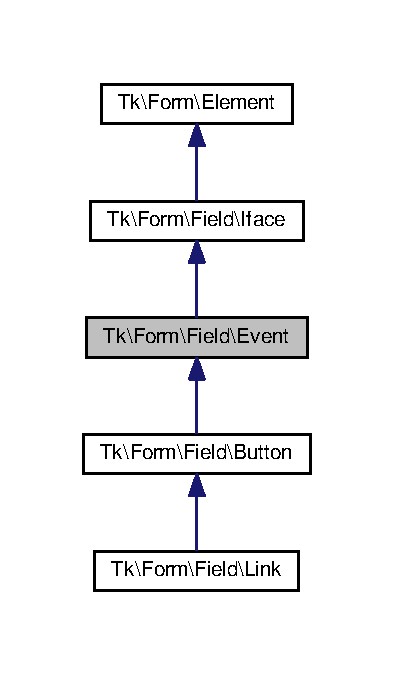
\includegraphics[width=189pt]{classTk_1_1Form_1_1Field_1_1Event__inherit__graph}
\end{center}
\end{figure}
\subsection*{Public Member Functions}
\begin{DoxyCompactItemize}
\item 
\hyperlink{classTk_1_1Form_1_1Field_1_1Event_a0574335765e57afd0cbb2d1ee99de99d}{\+\_\+\+\_\+construct} (\$name, \$callback=null)
\item 
\hyperlink{classTk_1_1Form_1_1Field_1_1Event_a0d582ec7ea4597127f314d765494d3d8}{get\+Callback} ()
\item 
\hyperlink{classTk_1_1Form_1_1Field_1_1Event_a15608a980278b92bb499c6ace2c8c7bd}{set\+Callback} (\$callback)
\end{DoxyCompactItemize}
\subsection*{Protected Attributes}
\begin{DoxyCompactItemize}
\item 
\hypertarget{classTk_1_1Form_1_1Field_1_1Event_a251cef167cb9d0e1f0c7fc92df4a6e92}{{\bfseries \$callback} = null}\label{classTk_1_1Form_1_1Field_1_1Event_a251cef167cb9d0e1f0c7fc92df4a6e92}

\end{DoxyCompactItemize}
\subsection*{Additional Inherited Members}


\subsection{Detailed Description}
Class Text

\begin{DoxyAuthor}{Author}
Michael Mifsud \href{mailto:info@tropotek.com}{\tt info@tropotek.\+com} \hyperlink{}{Copyright 2015 Michael Mifsud }
\end{DoxyAuthor}


\subsection{Constructor \& Destructor Documentation}
\hypertarget{classTk_1_1Form_1_1Field_1_1Event_a0574335765e57afd0cbb2d1ee99de99d}{\index{Tk\+::\+Form\+::\+Field\+::\+Event@{Tk\+::\+Form\+::\+Field\+::\+Event}!\+\_\+\+\_\+construct@{\+\_\+\+\_\+construct}}
\index{\+\_\+\+\_\+construct@{\+\_\+\+\_\+construct}!Tk\+::\+Form\+::\+Field\+::\+Event@{Tk\+::\+Form\+::\+Field\+::\+Event}}
\subsubsection[{\+\_\+\+\_\+construct}]{\setlength{\rightskip}{0pt plus 5cm}Tk\textbackslash{}\+Form\textbackslash{}\+Field\textbackslash{}\+Event\+::\+\_\+\+\_\+construct (
\begin{DoxyParamCaption}
\item[{}]{\$name, }
\item[{}]{\$callback = {\ttfamily null}}
\end{DoxyParamCaption}
)}}\label{classTk_1_1Form_1_1Field_1_1Event_a0574335765e57afd0cbb2d1ee99de99d}
\+\_\+\+\_\+construct


\begin{DoxyParams}[1]{Parameters}
string & {\em \$name} & \\
\hline
callable & {\em \$callback} & \\
\hline
\end{DoxyParams}


\subsection{Member Function Documentation}
\hypertarget{classTk_1_1Form_1_1Field_1_1Event_a0d582ec7ea4597127f314d765494d3d8}{\index{Tk\+::\+Form\+::\+Field\+::\+Event@{Tk\+::\+Form\+::\+Field\+::\+Event}!get\+Callback@{get\+Callback}}
\index{get\+Callback@{get\+Callback}!Tk\+::\+Form\+::\+Field\+::\+Event@{Tk\+::\+Form\+::\+Field\+::\+Event}}
\subsubsection[{get\+Callback}]{\setlength{\rightskip}{0pt plus 5cm}Tk\textbackslash{}\+Form\textbackslash{}\+Field\textbackslash{}\+Event\+::get\+Callback (
\begin{DoxyParamCaption}
{}
\end{DoxyParamCaption}
)}}\label{classTk_1_1Form_1_1Field_1_1Event_a0d582ec7ea4597127f314d765494d3d8}
get\+Event

\begin{DoxyReturn}{Returns}
callable 
\end{DoxyReturn}
\hypertarget{classTk_1_1Form_1_1Field_1_1Event_a15608a980278b92bb499c6ace2c8c7bd}{\index{Tk\+::\+Form\+::\+Field\+::\+Event@{Tk\+::\+Form\+::\+Field\+::\+Event}!set\+Callback@{set\+Callback}}
\index{set\+Callback@{set\+Callback}!Tk\+::\+Form\+::\+Field\+::\+Event@{Tk\+::\+Form\+::\+Field\+::\+Event}}
\subsubsection[{set\+Callback}]{\setlength{\rightskip}{0pt plus 5cm}Tk\textbackslash{}\+Form\textbackslash{}\+Field\textbackslash{}\+Event\+::set\+Callback (
\begin{DoxyParamCaption}
\item[{}]{\$callback}
\end{DoxyParamCaption}
)}}\label{classTk_1_1Form_1_1Field_1_1Event_a15608a980278b92bb499c6ace2c8c7bd}
set\+Event


\begin{DoxyParams}[1]{Parameters}
callable & {\em \$callback} & \\
\hline
\end{DoxyParams}
\begin{DoxyReturn}{Returns}
\$this 
\end{DoxyReturn}

\begin{DoxyExceptions}{Exceptions}
{\em } & Tk \\
\hline
\end{DoxyExceptions}


The documentation for this class was generated from the following file\+:\begin{DoxyCompactItemize}
\item 
vendor/ttek/tk-\/form/\+Tk/\+Form/\+Field/Event.\+php\end{DoxyCompactItemize}

\hypertarget{classTk_1_1Db_1_1Exception}{\section{Tk\textbackslash{}Db\textbackslash{}Exception Class Reference}
\label{classTk_1_1Db_1_1Exception}\index{Tk\textbackslash{}\+Db\textbackslash{}\+Exception@{Tk\textbackslash{}\+Db\textbackslash{}\+Exception}}
}


Inheritance diagram for Tk\textbackslash{}Db\textbackslash{}Exception\+:\nopagebreak
\begin{figure}[H]
\begin{center}
\leavevmode
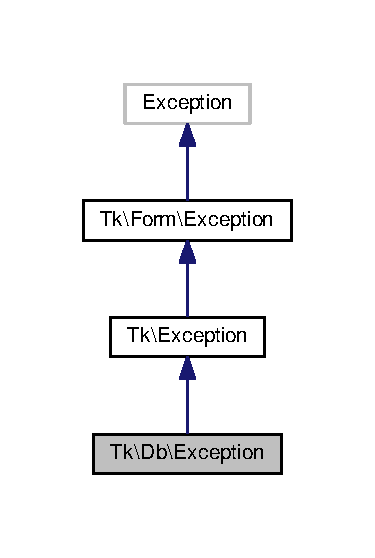
\includegraphics[width=180pt]{classTk_1_1Db_1_1Exception__inherit__graph}
\end{center}
\end{figure}
\subsection*{Public Member Functions}
\begin{DoxyCompactItemize}
\item 
\hyperlink{classTk_1_1Db_1_1Exception_aa129b85e66ddd994a55d253c366a6253}{set\+Dump} (\$dump)
\end{DoxyCompactItemize}
\subsection*{Additional Inherited Members}


\subsection{Detailed Description}
Class \hyperlink{classTk_1_1Db_1_1Exception}{Exception}

\begin{DoxyAuthor}{Author}
Michael Mifsud \href{mailto:info@tropotek.com}{\tt info@tropotek.\+com} \hyperlink{}{Copyright 2015 Michael Mifsud }
\end{DoxyAuthor}


\subsection{Member Function Documentation}
\hypertarget{classTk_1_1Db_1_1Exception_aa129b85e66ddd994a55d253c366a6253}{\index{Tk\+::\+Db\+::\+Exception@{Tk\+::\+Db\+::\+Exception}!set\+Dump@{set\+Dump}}
\index{set\+Dump@{set\+Dump}!Tk\+::\+Db\+::\+Exception@{Tk\+::\+Db\+::\+Exception}}
\subsubsection[{set\+Dump}]{\setlength{\rightskip}{0pt plus 5cm}Tk\textbackslash{}\+Db\textbackslash{}\+Exception\+::set\+Dump (
\begin{DoxyParamCaption}
\item[{}]{\$dump}
\end{DoxyParamCaption}
)}}\label{classTk_1_1Db_1_1Exception_aa129b85e66ddd994a55d253c366a6253}
Set any memory, code dump data to display in the eception error


\begin{DoxyParams}[1]{Parameters}
string & {\em \$dump} & \\
\hline
\end{DoxyParams}


The documentation for this class was generated from the following file\+:\begin{DoxyCompactItemize}
\item 
vendor/ttek/tk-\/framework/\+Tk/\+Db/Exception.\+php\end{DoxyCompactItemize}

\hypertarget{classTk_1_1Dom_1_1Modifier_1_1Exception}{\section{Tk\textbackslash{}Dom\textbackslash{}Modifier\textbackslash{}Exception Class Reference}
\label{classTk_1_1Dom_1_1Modifier_1_1Exception}\index{Tk\textbackslash{}\+Dom\textbackslash{}\+Modifier\textbackslash{}\+Exception@{Tk\textbackslash{}\+Dom\textbackslash{}\+Modifier\textbackslash{}\+Exception}}
}


Inheritance diagram for Tk\textbackslash{}Dom\textbackslash{}Modifier\textbackslash{}Exception\+:\nopagebreak
\begin{figure}[H]
\begin{center}
\leavevmode
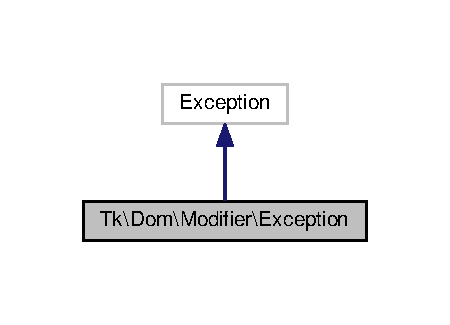
\includegraphics[width=216pt]{classTk_1_1Dom_1_1Modifier_1_1Exception__inherit__graph}
\end{center}
\end{figure}


\subsection{Detailed Description}
Class \hyperlink{classTk_1_1Dom_1_1Modifier_1_1Exception}{Exception}

\begin{DoxyAuthor}{Author}
Michael Mifsud \href{mailto:info@tropotek.com}{\tt info@tropotek.\+com} \hyperlink{}{Copyright 2007 Michael Mifsud }
\end{DoxyAuthor}


The documentation for this class was generated from the following file\+:\begin{DoxyCompactItemize}
\item 
vendor/ttek/tk-\/framework/\+Tk/\+Dom/\+Modifier/Exception.\+php\end{DoxyCompactItemize}

\hypertarget{classTk_1_1Exception}{\section{Tk\textbackslash{}Exception Class Reference}
\label{classTk_1_1Exception}\index{Tk\textbackslash{}\+Exception@{Tk\textbackslash{}\+Exception}}
}


Inheritance diagram for Tk\textbackslash{}Exception\+:\nopagebreak
\begin{figure}[H]
\begin{center}
\leavevmode
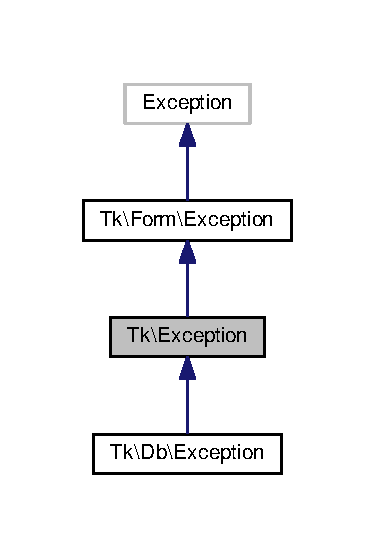
\includegraphics[width=180pt]{classTk_1_1Exception__inherit__graph}
\end{center}
\end{figure}
\subsection*{Public Member Functions}
\begin{DoxyCompactItemize}
\item 
\hyperlink{classTk_1_1Exception_ae0530af4a6ee6013addf3bf1aa6e8074}{set\+Dump} (\$dump)
\item 
\hyperlink{classTk_1_1Exception_aef26c3043785b1af9d850dd7ba278069}{\+\_\+\+\_\+to\+String} ()
\end{DoxyCompactItemize}
\subsection*{Protected Attributes}
\begin{DoxyCompactItemize}
\item 
\hypertarget{classTk_1_1Exception_a7723ab708d93d05f5b380dab1af6efe4}{{\bfseries \$dump} = ''}\label{classTk_1_1Exception_a7723ab708d93d05f5b380dab1af6efe4}

\end{DoxyCompactItemize}


\subsection{Detailed Description}
Class \hyperlink{classTk_1_1Exception}{Exception}

\begin{DoxyAuthor}{Author}
Michael Mifsud \href{mailto:info@tropotek.com}{\tt info@tropotek.\+com} \hyperlink{}{Copyright 2007 Michael Mifsud }
\end{DoxyAuthor}


\subsection{Member Function Documentation}
\hypertarget{classTk_1_1Exception_aef26c3043785b1af9d850dd7ba278069}{\index{Tk\+::\+Exception@{Tk\+::\+Exception}!\+\_\+\+\_\+to\+String@{\+\_\+\+\_\+to\+String}}
\index{\+\_\+\+\_\+to\+String@{\+\_\+\+\_\+to\+String}!Tk\+::\+Exception@{Tk\+::\+Exception}}
\subsubsection[{\+\_\+\+\_\+to\+String}]{\setlength{\rightskip}{0pt plus 5cm}Tk\textbackslash{}\+Exception\+::\+\_\+\+\_\+to\+String (
\begin{DoxyParamCaption}
{}
\end{DoxyParamCaption}
)}}\label{classTk_1_1Exception_aef26c3043785b1af9d850dd7ba278069}
(P\+H\+P 5 $>$= 5.\+1.\+0)~\newline
 String representation of the exception \hyperlink{}{string the string representation of the exception. }\hypertarget{classTk_1_1Exception_ae0530af4a6ee6013addf3bf1aa6e8074}{\index{Tk\+::\+Exception@{Tk\+::\+Exception}!set\+Dump@{set\+Dump}}
\index{set\+Dump@{set\+Dump}!Tk\+::\+Exception@{Tk\+::\+Exception}}
\subsubsection[{set\+Dump}]{\setlength{\rightskip}{0pt plus 5cm}Tk\textbackslash{}\+Exception\+::set\+Dump (
\begin{DoxyParamCaption}
\item[{}]{\$dump}
\end{DoxyParamCaption}
)}}\label{classTk_1_1Exception_ae0530af4a6ee6013addf3bf1aa6e8074}
Set any memory, code dump data to display in the exception error


\begin{DoxyParams}[1]{Parameters}
string & {\em \$dump} & \\
\hline
\end{DoxyParams}


The documentation for this class was generated from the following file\+:\begin{DoxyCompactItemize}
\item 
vendor/ttek/tk-\/framework/\+Tk/Exception.\+php\end{DoxyCompactItemize}

\hypertarget{classDom_1_1Exception}{\section{Dom\textbackslash{}Exception Class Reference}
\label{classDom_1_1Exception}\index{Dom\textbackslash{}\+Exception@{Dom\textbackslash{}\+Exception}}
}


Inheritance diagram for Dom\textbackslash{}Exception\+:\nopagebreak
\begin{figure}[H]
\begin{center}
\leavevmode
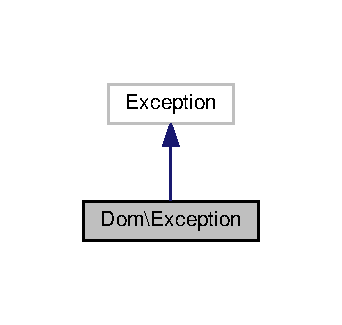
\includegraphics[width=164pt]{classDom_1_1Exception__inherit__graph}
\end{center}
\end{figure}


\subsection{Detailed Description}
Class \hyperlink{classDom_1_1Exception}{Exception}

\begin{DoxyAuthor}{Author}
Michael Mifsud \href{mailto:info@tropotek.com}{\tt info@tropotek.\+com} \hyperlink{}{Copyright 2007 Michael Mifsud }
\end{DoxyAuthor}


The documentation for this class was generated from the following file\+:\begin{DoxyCompactItemize}
\item 
vendor/ttek/tk-\/domtemplate/\+Dom/Exception.\+php\end{DoxyCompactItemize}

\hypertarget{classTk_1_1Table_1_1Exception}{\section{Tk\textbackslash{}Table\textbackslash{}Exception Class Reference}
\label{classTk_1_1Table_1_1Exception}\index{Tk\textbackslash{}\+Table\textbackslash{}\+Exception@{Tk\textbackslash{}\+Table\textbackslash{}\+Exception}}
}


Inheritance diagram for Tk\textbackslash{}Table\textbackslash{}Exception\+:\nopagebreak
\begin{figure}[H]
\begin{center}
\leavevmode
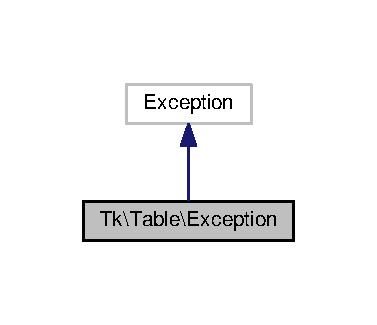
\includegraphics[width=181pt]{classTk_1_1Table_1_1Exception__inherit__graph}
\end{center}
\end{figure}


\subsection{Detailed Description}
Class \hyperlink{classTk_1_1Table_1_1Exception}{Exception}

\begin{DoxyAuthor}{Author}
Michael Mifsud \href{mailto:info@tropotek.com}{\tt info@tropotek.\+com} \hyperlink{}{Copyright 2015 Michael Mifsud }
\end{DoxyAuthor}


The documentation for this class was generated from the following file\+:\begin{DoxyCompactItemize}
\item 
vendor/ttek/tk-\/table/\+Tk/\+Table/Exception.\+php\end{DoxyCompactItemize}

\hypertarget{classTk_1_1Form_1_1Exception}{\section{Tk\textbackslash{}Form\textbackslash{}Exception Class Reference}
\label{classTk_1_1Form_1_1Exception}\index{Tk\textbackslash{}\+Form\textbackslash{}\+Exception@{Tk\textbackslash{}\+Form\textbackslash{}\+Exception}}
}


Inheritance diagram for Tk\textbackslash{}Form\textbackslash{}Exception\+:\nopagebreak
\begin{figure}[H]
\begin{center}
\leavevmode
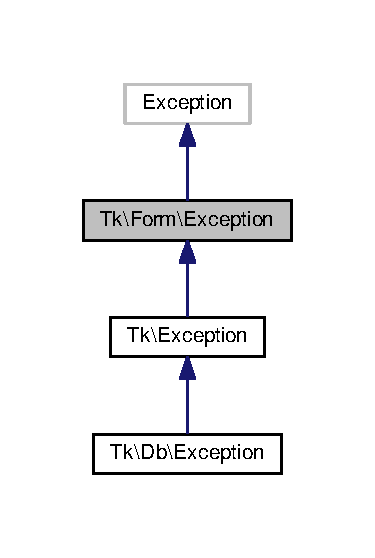
\includegraphics[width=180pt]{classTk_1_1Form_1_1Exception__inherit__graph}
\end{center}
\end{figure}


\subsection{Detailed Description}
Class \hyperlink{classTk_1_1Form_1_1Exception}{Exception}

\begin{DoxyAuthor}{Author}
Michael Mifsud \href{mailto:info@tropotek.com}{\tt info@tropotek.\+com} \hyperlink{}{Copyright 2015 Michael Mifsud }
\end{DoxyAuthor}


The documentation for this class was generated from the following file\+:\begin{DoxyCompactItemize}
\item 
vendor/ttek/tk-\/form/\+Tk/\+Form/Exception.\+php\end{DoxyCompactItemize}

\hypertarget{classTk_1_1Form_1_1Renderer_1_1Dom_1_1FieldFactory}{\section{Tk\textbackslash{}Form\textbackslash{}Renderer\textbackslash{}Dom\textbackslash{}Field\+Factory Class Reference}
\label{classTk_1_1Form_1_1Renderer_1_1Dom_1_1FieldFactory}\index{Tk\textbackslash{}\+Form\textbackslash{}\+Renderer\textbackslash{}\+Dom\textbackslash{}\+Field\+Factory@{Tk\textbackslash{}\+Form\textbackslash{}\+Renderer\textbackslash{}\+Dom\textbackslash{}\+Field\+Factory}}
}
\subsection*{Static Public Member Functions}
\begin{DoxyCompactItemize}
\item 
static \hyperlink{classTk_1_1Form_1_1Renderer_1_1Dom_1_1FieldFactory_af040360732a6f718cb37c5d553e8b75a}{create\+Button} (\$name, \$callback=null)
\item 
static \hyperlink{classTk_1_1Form_1_1Renderer_1_1Dom_1_1FieldFactory_a844ded032cbf88dcf38dbbc57eb4296d}{create\+Checkbox} (\$name)
\item 
static \hyperlink{classTk_1_1Form_1_1Renderer_1_1Dom_1_1FieldFactory_a560d4e66e5a12116661b33f907e1f9cb}{create\+Date} (\$name)
\item 
static \hyperlink{classTk_1_1Form_1_1Renderer_1_1Dom_1_1FieldFactory_ac1f64af89135b5536c4d309cb7b20afc}{create\+File} (\$name)
\item 
static \hyperlink{classTk_1_1Form_1_1Renderer_1_1Dom_1_1FieldFactory_a71c0395cf1a28816c2723c34110a3d7c}{create\+Hidden} (\$name)
\item 
static \hyperlink{classTk_1_1Form_1_1Renderer_1_1Dom_1_1FieldFactory_a75aee22954c35e5871ba83cd2148a80a}{create\+Link} (\$name, \$url=null, \$callback=null)
\item 
static \hyperlink{classTk_1_1Form_1_1Renderer_1_1Dom_1_1FieldFactory_ac6f6223672fb99dfa38afb38878549c4}{create\+Password} (\$name)
\item 
static \hyperlink{classTk_1_1Form_1_1Renderer_1_1Dom_1_1FieldFactory_a87f8523f33dfa1d16d0228792633ba72}{create\+Html} (\$name, \$html)
\item 
static \hyperlink{classTk_1_1Form_1_1Renderer_1_1Dom_1_1FieldFactory_a3b86a7173ff38a4771ef87b9b66c1b20}{create\+Select} (\$name, \$option\+Iterator=null)
\item 
static \hyperlink{classTk_1_1Form_1_1Renderer_1_1Dom_1_1FieldFactory_a8ada246d469ffb310bcd01ca365c5b30}{create\+Text} (\$name)
\item 
static \hyperlink{classTk_1_1Form_1_1Renderer_1_1Dom_1_1FieldFactory_aaf153174eee3f6deadefe6e7ba539b7e}{create\+Textarea} (\$name)
\end{DoxyCompactItemize}


\subsection{Detailed Description}
Class \hyperlink{classTk_1_1Form_1_1Renderer_1_1Dom_1_1FieldFactory}{Field\+Factory}

\begin{DoxyAuthor}{Author}
Michael Mifsud \href{mailto:info@tropotek.com}{\tt info@tropotek.\+com} \hyperlink{}{Copyright 2015 Michael Mifsud }
\end{DoxyAuthor}


\subsection{Member Function Documentation}
\hypertarget{classTk_1_1Form_1_1Renderer_1_1Dom_1_1FieldFactory_af040360732a6f718cb37c5d553e8b75a}{\index{Tk\+::\+Form\+::\+Renderer\+::\+Dom\+::\+Field\+Factory@{Tk\+::\+Form\+::\+Renderer\+::\+Dom\+::\+Field\+Factory}!create\+Button@{create\+Button}}
\index{create\+Button@{create\+Button}!Tk\+::\+Form\+::\+Renderer\+::\+Dom\+::\+Field\+Factory@{Tk\+::\+Form\+::\+Renderer\+::\+Dom\+::\+Field\+Factory}}
\subsubsection[{create\+Button}]{\setlength{\rightskip}{0pt plus 5cm}static Tk\textbackslash{}\+Form\textbackslash{}\+Renderer\textbackslash{}\+Dom\textbackslash{}\+Field\+Factory\+::create\+Button (
\begin{DoxyParamCaption}
\item[{}]{\$name, }
\item[{}]{\$callback = {\ttfamily null}}
\end{DoxyParamCaption}
)\hspace{0.3cm}{\ttfamily [static]}}}\label{classTk_1_1Form_1_1Renderer_1_1Dom_1_1FieldFactory_af040360732a6f718cb37c5d553e8b75a}
Create A Field


\begin{DoxyParams}[1]{Parameters}
string & {\em \$name} & \\
\hline
callable & {\em \$callback} & \\
\hline
\end{DoxyParams}
\begin{DoxyReturn}{Returns}

\end{DoxyReturn}
\hypertarget{classTk_1_1Form_1_1Renderer_1_1Dom_1_1FieldFactory_a844ded032cbf88dcf38dbbc57eb4296d}{\index{Tk\+::\+Form\+::\+Renderer\+::\+Dom\+::\+Field\+Factory@{Tk\+::\+Form\+::\+Renderer\+::\+Dom\+::\+Field\+Factory}!create\+Checkbox@{create\+Checkbox}}
\index{create\+Checkbox@{create\+Checkbox}!Tk\+::\+Form\+::\+Renderer\+::\+Dom\+::\+Field\+Factory@{Tk\+::\+Form\+::\+Renderer\+::\+Dom\+::\+Field\+Factory}}
\subsubsection[{create\+Checkbox}]{\setlength{\rightskip}{0pt plus 5cm}static Tk\textbackslash{}\+Form\textbackslash{}\+Renderer\textbackslash{}\+Dom\textbackslash{}\+Field\+Factory\+::create\+Checkbox (
\begin{DoxyParamCaption}
\item[{}]{\$name}
\end{DoxyParamCaption}
)\hspace{0.3cm}{\ttfamily [static]}}}\label{classTk_1_1Form_1_1Renderer_1_1Dom_1_1FieldFactory_a844ded032cbf88dcf38dbbc57eb4296d}
Create A Field


\begin{DoxyParams}[1]{Parameters}
string & {\em \$name} & \\
\hline
\end{DoxyParams}
\begin{DoxyReturn}{Returns}

\end{DoxyReturn}
\hypertarget{classTk_1_1Form_1_1Renderer_1_1Dom_1_1FieldFactory_a560d4e66e5a12116661b33f907e1f9cb}{\index{Tk\+::\+Form\+::\+Renderer\+::\+Dom\+::\+Field\+Factory@{Tk\+::\+Form\+::\+Renderer\+::\+Dom\+::\+Field\+Factory}!create\+Date@{create\+Date}}
\index{create\+Date@{create\+Date}!Tk\+::\+Form\+::\+Renderer\+::\+Dom\+::\+Field\+Factory@{Tk\+::\+Form\+::\+Renderer\+::\+Dom\+::\+Field\+Factory}}
\subsubsection[{create\+Date}]{\setlength{\rightskip}{0pt plus 5cm}static Tk\textbackslash{}\+Form\textbackslash{}\+Renderer\textbackslash{}\+Dom\textbackslash{}\+Field\+Factory\+::create\+Date (
\begin{DoxyParamCaption}
\item[{}]{\$name}
\end{DoxyParamCaption}
)\hspace{0.3cm}{\ttfamily [static]}}}\label{classTk_1_1Form_1_1Renderer_1_1Dom_1_1FieldFactory_a560d4e66e5a12116661b33f907e1f9cb}
Create A Field


\begin{DoxyParams}[1]{Parameters}
string & {\em \$name} & \\
\hline
\end{DoxyParams}
\begin{DoxyReturn}{Returns}

\end{DoxyReturn}
\hypertarget{classTk_1_1Form_1_1Renderer_1_1Dom_1_1FieldFactory_ac1f64af89135b5536c4d309cb7b20afc}{\index{Tk\+::\+Form\+::\+Renderer\+::\+Dom\+::\+Field\+Factory@{Tk\+::\+Form\+::\+Renderer\+::\+Dom\+::\+Field\+Factory}!create\+File@{create\+File}}
\index{create\+File@{create\+File}!Tk\+::\+Form\+::\+Renderer\+::\+Dom\+::\+Field\+Factory@{Tk\+::\+Form\+::\+Renderer\+::\+Dom\+::\+Field\+Factory}}
\subsubsection[{create\+File}]{\setlength{\rightskip}{0pt plus 5cm}static Tk\textbackslash{}\+Form\textbackslash{}\+Renderer\textbackslash{}\+Dom\textbackslash{}\+Field\+Factory\+::create\+File (
\begin{DoxyParamCaption}
\item[{}]{\$name}
\end{DoxyParamCaption}
)\hspace{0.3cm}{\ttfamily [static]}}}\label{classTk_1_1Form_1_1Renderer_1_1Dom_1_1FieldFactory_ac1f64af89135b5536c4d309cb7b20afc}
Create A Field


\begin{DoxyParams}[1]{Parameters}
string & {\em \$name} & \\
\hline
\end{DoxyParams}
\begin{DoxyReturn}{Returns}

\end{DoxyReturn}
\hypertarget{classTk_1_1Form_1_1Renderer_1_1Dom_1_1FieldFactory_a71c0395cf1a28816c2723c34110a3d7c}{\index{Tk\+::\+Form\+::\+Renderer\+::\+Dom\+::\+Field\+Factory@{Tk\+::\+Form\+::\+Renderer\+::\+Dom\+::\+Field\+Factory}!create\+Hidden@{create\+Hidden}}
\index{create\+Hidden@{create\+Hidden}!Tk\+::\+Form\+::\+Renderer\+::\+Dom\+::\+Field\+Factory@{Tk\+::\+Form\+::\+Renderer\+::\+Dom\+::\+Field\+Factory}}
\subsubsection[{create\+Hidden}]{\setlength{\rightskip}{0pt plus 5cm}static Tk\textbackslash{}\+Form\textbackslash{}\+Renderer\textbackslash{}\+Dom\textbackslash{}\+Field\+Factory\+::create\+Hidden (
\begin{DoxyParamCaption}
\item[{}]{\$name}
\end{DoxyParamCaption}
)\hspace{0.3cm}{\ttfamily [static]}}}\label{classTk_1_1Form_1_1Renderer_1_1Dom_1_1FieldFactory_a71c0395cf1a28816c2723c34110a3d7c}
Create A Field


\begin{DoxyParams}[1]{Parameters}
string & {\em \$name} & \\
\hline
\end{DoxyParams}
\begin{DoxyReturn}{Returns}

\end{DoxyReturn}
\hypertarget{classTk_1_1Form_1_1Renderer_1_1Dom_1_1FieldFactory_a87f8523f33dfa1d16d0228792633ba72}{\index{Tk\+::\+Form\+::\+Renderer\+::\+Dom\+::\+Field\+Factory@{Tk\+::\+Form\+::\+Renderer\+::\+Dom\+::\+Field\+Factory}!create\+Html@{create\+Html}}
\index{create\+Html@{create\+Html}!Tk\+::\+Form\+::\+Renderer\+::\+Dom\+::\+Field\+Factory@{Tk\+::\+Form\+::\+Renderer\+::\+Dom\+::\+Field\+Factory}}
\subsubsection[{create\+Html}]{\setlength{\rightskip}{0pt plus 5cm}static Tk\textbackslash{}\+Form\textbackslash{}\+Renderer\textbackslash{}\+Dom\textbackslash{}\+Field\+Factory\+::create\+Html (
\begin{DoxyParamCaption}
\item[{}]{\$name, }
\item[{}]{\$html}
\end{DoxyParamCaption}
)\hspace{0.3cm}{\ttfamily [static]}}}\label{classTk_1_1Form_1_1Renderer_1_1Dom_1_1FieldFactory_a87f8523f33dfa1d16d0228792633ba72}
Create A Field


\begin{DoxyParams}[1]{Parameters}
string & {\em \$name} & \\
\hline
\end{DoxyParams}
\begin{DoxyReturn}{Returns}

\end{DoxyReturn}
\hypertarget{classTk_1_1Form_1_1Renderer_1_1Dom_1_1FieldFactory_a75aee22954c35e5871ba83cd2148a80a}{\index{Tk\+::\+Form\+::\+Renderer\+::\+Dom\+::\+Field\+Factory@{Tk\+::\+Form\+::\+Renderer\+::\+Dom\+::\+Field\+Factory}!create\+Link@{create\+Link}}
\index{create\+Link@{create\+Link}!Tk\+::\+Form\+::\+Renderer\+::\+Dom\+::\+Field\+Factory@{Tk\+::\+Form\+::\+Renderer\+::\+Dom\+::\+Field\+Factory}}
\subsubsection[{create\+Link}]{\setlength{\rightskip}{0pt plus 5cm}static Tk\textbackslash{}\+Form\textbackslash{}\+Renderer\textbackslash{}\+Dom\textbackslash{}\+Field\+Factory\+::create\+Link (
\begin{DoxyParamCaption}
\item[{}]{\$name, }
\item[{}]{\$url = {\ttfamily null}, }
\item[{}]{\$callback = {\ttfamily null}}
\end{DoxyParamCaption}
)\hspace{0.3cm}{\ttfamily [static]}}}\label{classTk_1_1Form_1_1Renderer_1_1Dom_1_1FieldFactory_a75aee22954c35e5871ba83cd2148a80a}
Create A Field


\begin{DoxyParams}[1]{Parameters}
string & {\em \$name} & \\
\hline
string | \textbackslash{}\+Tk\textbackslash{}\+Url & {\em \$url} & \\
\hline
callable & {\em \$callback} & \\
\hline
\end{DoxyParams}
\begin{DoxyReturn}{Returns}

\end{DoxyReturn}
\hypertarget{classTk_1_1Form_1_1Renderer_1_1Dom_1_1FieldFactory_ac6f6223672fb99dfa38afb38878549c4}{\index{Tk\+::\+Form\+::\+Renderer\+::\+Dom\+::\+Field\+Factory@{Tk\+::\+Form\+::\+Renderer\+::\+Dom\+::\+Field\+Factory}!create\+Password@{create\+Password}}
\index{create\+Password@{create\+Password}!Tk\+::\+Form\+::\+Renderer\+::\+Dom\+::\+Field\+Factory@{Tk\+::\+Form\+::\+Renderer\+::\+Dom\+::\+Field\+Factory}}
\subsubsection[{create\+Password}]{\setlength{\rightskip}{0pt plus 5cm}static Tk\textbackslash{}\+Form\textbackslash{}\+Renderer\textbackslash{}\+Dom\textbackslash{}\+Field\+Factory\+::create\+Password (
\begin{DoxyParamCaption}
\item[{}]{\$name}
\end{DoxyParamCaption}
)\hspace{0.3cm}{\ttfamily [static]}}}\label{classTk_1_1Form_1_1Renderer_1_1Dom_1_1FieldFactory_ac6f6223672fb99dfa38afb38878549c4}
Create A Field


\begin{DoxyParams}[1]{Parameters}
string & {\em \$name} & \\
\hline
\end{DoxyParams}
\begin{DoxyReturn}{Returns}

\end{DoxyReturn}
\hypertarget{classTk_1_1Form_1_1Renderer_1_1Dom_1_1FieldFactory_a3b86a7173ff38a4771ef87b9b66c1b20}{\index{Tk\+::\+Form\+::\+Renderer\+::\+Dom\+::\+Field\+Factory@{Tk\+::\+Form\+::\+Renderer\+::\+Dom\+::\+Field\+Factory}!create\+Select@{create\+Select}}
\index{create\+Select@{create\+Select}!Tk\+::\+Form\+::\+Renderer\+::\+Dom\+::\+Field\+Factory@{Tk\+::\+Form\+::\+Renderer\+::\+Dom\+::\+Field\+Factory}}
\subsubsection[{create\+Select}]{\setlength{\rightskip}{0pt plus 5cm}static Tk\textbackslash{}\+Form\textbackslash{}\+Renderer\textbackslash{}\+Dom\textbackslash{}\+Field\+Factory\+::create\+Select (
\begin{DoxyParamCaption}
\item[{}]{\$name, }
\item[{}]{\$option\+Iterator = {\ttfamily null}}
\end{DoxyParamCaption}
)\hspace{0.3cm}{\ttfamily [static]}}}\label{classTk_1_1Form_1_1Renderer_1_1Dom_1_1FieldFactory_a3b86a7173ff38a4771ef87b9b66c1b20}
Create A Field


\begin{DoxyParams}[1]{Parameters}
string & {\em \$name} & \\
\hline
\textbackslash{}\+Tk\textbackslash{}\+Form\textbackslash{}\+Field\textbackslash{}\+Option\textbackslash{}\+Array\+Iterator & {\em \$option\+Iterator} & \\
\hline
\end{DoxyParams}
\begin{DoxyReturn}{Returns}

\end{DoxyReturn}
\hypertarget{classTk_1_1Form_1_1Renderer_1_1Dom_1_1FieldFactory_a8ada246d469ffb310bcd01ca365c5b30}{\index{Tk\+::\+Form\+::\+Renderer\+::\+Dom\+::\+Field\+Factory@{Tk\+::\+Form\+::\+Renderer\+::\+Dom\+::\+Field\+Factory}!create\+Text@{create\+Text}}
\index{create\+Text@{create\+Text}!Tk\+::\+Form\+::\+Renderer\+::\+Dom\+::\+Field\+Factory@{Tk\+::\+Form\+::\+Renderer\+::\+Dom\+::\+Field\+Factory}}
\subsubsection[{create\+Text}]{\setlength{\rightskip}{0pt plus 5cm}static Tk\textbackslash{}\+Form\textbackslash{}\+Renderer\textbackslash{}\+Dom\textbackslash{}\+Field\+Factory\+::create\+Text (
\begin{DoxyParamCaption}
\item[{}]{\$name}
\end{DoxyParamCaption}
)\hspace{0.3cm}{\ttfamily [static]}}}\label{classTk_1_1Form_1_1Renderer_1_1Dom_1_1FieldFactory_a8ada246d469ffb310bcd01ca365c5b30}
Create A Field


\begin{DoxyParams}[1]{Parameters}
string & {\em \$name} & \\
\hline
\end{DoxyParams}
\begin{DoxyReturn}{Returns}

\end{DoxyReturn}
\hypertarget{classTk_1_1Form_1_1Renderer_1_1Dom_1_1FieldFactory_aaf153174eee3f6deadefe6e7ba539b7e}{\index{Tk\+::\+Form\+::\+Renderer\+::\+Dom\+::\+Field\+Factory@{Tk\+::\+Form\+::\+Renderer\+::\+Dom\+::\+Field\+Factory}!create\+Textarea@{create\+Textarea}}
\index{create\+Textarea@{create\+Textarea}!Tk\+::\+Form\+::\+Renderer\+::\+Dom\+::\+Field\+Factory@{Tk\+::\+Form\+::\+Renderer\+::\+Dom\+::\+Field\+Factory}}
\subsubsection[{create\+Textarea}]{\setlength{\rightskip}{0pt plus 5cm}static Tk\textbackslash{}\+Form\textbackslash{}\+Renderer\textbackslash{}\+Dom\textbackslash{}\+Field\+Factory\+::create\+Textarea (
\begin{DoxyParamCaption}
\item[{}]{\$name}
\end{DoxyParamCaption}
)\hspace{0.3cm}{\ttfamily [static]}}}\label{classTk_1_1Form_1_1Renderer_1_1Dom_1_1FieldFactory_aaf153174eee3f6deadefe6e7ba539b7e}
Create A Field


\begin{DoxyParams}[1]{Parameters}
string & {\em \$name} & \\
\hline
\end{DoxyParams}
\begin{DoxyReturn}{Returns}

\end{DoxyReturn}


The documentation for this class was generated from the following file\+:\begin{DoxyCompactItemize}
\item 
vendor/ttek/tk-\/form/\+Tk/\+Form/\+Renderer/\+Dom/Field\+Factory.\+php\end{DoxyCompactItemize}

\hypertarget{classTk_1_1Form_1_1Renderer_1_1Dom_1_1FieldGroup}{\section{Tk\textbackslash{}Form\textbackslash{}Renderer\textbackslash{}Dom\textbackslash{}Field\+Group Class Reference}
\label{classTk_1_1Form_1_1Renderer_1_1Dom_1_1FieldGroup}\index{Tk\textbackslash{}\+Form\textbackslash{}\+Renderer\textbackslash{}\+Dom\textbackslash{}\+Field\+Group@{Tk\textbackslash{}\+Form\textbackslash{}\+Renderer\textbackslash{}\+Dom\textbackslash{}\+Field\+Group}}
}


Inheritance diagram for Tk\textbackslash{}Form\textbackslash{}Renderer\textbackslash{}Dom\textbackslash{}Field\+Group\+:\nopagebreak
\begin{figure}[H]
\begin{center}
\leavevmode
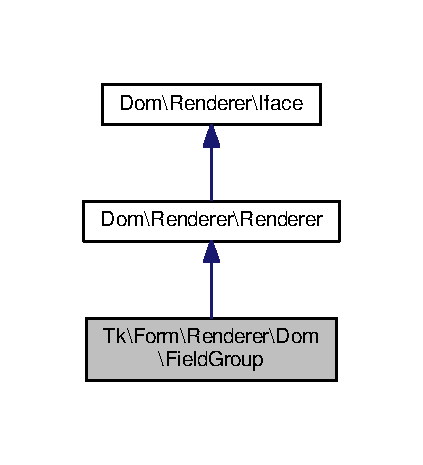
\includegraphics[width=203pt]{classTk_1_1Form_1_1Renderer_1_1Dom_1_1FieldGroup__inherit__graph}
\end{center}
\end{figure}
\subsection*{Public Member Functions}
\begin{DoxyCompactItemize}
\item 
\hyperlink{classTk_1_1Form_1_1Renderer_1_1Dom_1_1FieldGroup_ae49eb741ccb71564277601a8c08d2268}{\+\_\+\+\_\+construct} (\$field\+Renderer)
\item 
\hyperlink{classTk_1_1Form_1_1Renderer_1_1Dom_1_1FieldGroup_a3c53fa1a5be67558d74e76d2f1820087}{get\+Field\+Renderer} ()
\item 
\hyperlink{classTk_1_1Form_1_1Renderer_1_1Dom_1_1FieldGroup_afd18726c000171d11abfd6044d1e3b01}{show} ()
\end{DoxyCompactItemize}
\subsection*{Static Public Member Functions}
\begin{DoxyCompactItemize}
\item 
static \hyperlink{classTk_1_1Form_1_1Renderer_1_1Dom_1_1FieldGroup_aa1013df31e1b017649d80ce0c3ac5b0c}{create} (\$field\+Renderer)
\end{DoxyCompactItemize}
\subsection*{Protected Member Functions}
\begin{DoxyCompactItemize}
\item 
\hyperlink{classTk_1_1Form_1_1Renderer_1_1Dom_1_1FieldGroup_a2455b4a6397f974eafc80e8867b8317f}{\+\_\+\+\_\+make\+Template} ()
\end{DoxyCompactItemize}
\subsection*{Protected Attributes}
\begin{DoxyCompactItemize}
\item 
\hypertarget{classTk_1_1Form_1_1Renderer_1_1Dom_1_1FieldGroup_a039034321cda33c40f800946faa02955}{{\bfseries \$field\+Renderer} = null}\label{classTk_1_1Form_1_1Renderer_1_1Dom_1_1FieldGroup_a039034321cda33c40f800946faa02955}

\end{DoxyCompactItemize}


\subsection{Detailed Description}
Class Field\+Renderer

\begin{DoxyAuthor}{Author}
Michael Mifsud \href{mailto:info@tropotek.com}{\tt info@tropotek.\+com} \hyperlink{}{Copyright 2015 Michael Mifsud }
\end{DoxyAuthor}


\subsection{Constructor \& Destructor Documentation}
\hypertarget{classTk_1_1Form_1_1Renderer_1_1Dom_1_1FieldGroup_ae49eb741ccb71564277601a8c08d2268}{\index{Tk\+::\+Form\+::\+Renderer\+::\+Dom\+::\+Field\+Group@{Tk\+::\+Form\+::\+Renderer\+::\+Dom\+::\+Field\+Group}!\+\_\+\+\_\+construct@{\+\_\+\+\_\+construct}}
\index{\+\_\+\+\_\+construct@{\+\_\+\+\_\+construct}!Tk\+::\+Form\+::\+Renderer\+::\+Dom\+::\+Field\+Group@{Tk\+::\+Form\+::\+Renderer\+::\+Dom\+::\+Field\+Group}}
\subsubsection[{\+\_\+\+\_\+construct}]{\setlength{\rightskip}{0pt plus 5cm}Tk\textbackslash{}\+Form\textbackslash{}\+Renderer\textbackslash{}\+Dom\textbackslash{}\+Field\+Group\+::\+\_\+\+\_\+construct (
\begin{DoxyParamCaption}
\item[{}]{\$field\+Renderer}
\end{DoxyParamCaption}
)}}\label{classTk_1_1Form_1_1Renderer_1_1Dom_1_1FieldGroup_ae49eb741ccb71564277601a8c08d2268}
\+\_\+\+\_\+construct


\begin{DoxyParams}[1]{Parameters}
Field\textbackslash{}\+Iface & {\em \$field\+Renderer} & \\
\hline
\end{DoxyParams}


\subsection{Member Function Documentation}
\hypertarget{classTk_1_1Form_1_1Renderer_1_1Dom_1_1FieldGroup_a2455b4a6397f974eafc80e8867b8317f}{\index{Tk\+::\+Form\+::\+Renderer\+::\+Dom\+::\+Field\+Group@{Tk\+::\+Form\+::\+Renderer\+::\+Dom\+::\+Field\+Group}!\+\_\+\+\_\+make\+Template@{\+\_\+\+\_\+make\+Template}}
\index{\+\_\+\+\_\+make\+Template@{\+\_\+\+\_\+make\+Template}!Tk\+::\+Form\+::\+Renderer\+::\+Dom\+::\+Field\+Group@{Tk\+::\+Form\+::\+Renderer\+::\+Dom\+::\+Field\+Group}}
\subsubsection[{\+\_\+\+\_\+make\+Template}]{\setlength{\rightskip}{0pt plus 5cm}Tk\textbackslash{}\+Form\textbackslash{}\+Renderer\textbackslash{}\+Dom\textbackslash{}\+Field\+Group\+::\+\_\+\+\_\+make\+Template (
\begin{DoxyParamCaption}
{}
\end{DoxyParamCaption}
)\hspace{0.3cm}{\ttfamily [protected]}}}\label{classTk_1_1Form_1_1Renderer_1_1Dom_1_1FieldGroup_a2455b4a6397f974eafc80e8867b8317f}
make\+Template

\begin{DoxyReturn}{Returns}
string 
\end{DoxyReturn}
\hypertarget{classTk_1_1Form_1_1Renderer_1_1Dom_1_1FieldGroup_aa1013df31e1b017649d80ce0c3ac5b0c}{\index{Tk\+::\+Form\+::\+Renderer\+::\+Dom\+::\+Field\+Group@{Tk\+::\+Form\+::\+Renderer\+::\+Dom\+::\+Field\+Group}!create@{create}}
\index{create@{create}!Tk\+::\+Form\+::\+Renderer\+::\+Dom\+::\+Field\+Group@{Tk\+::\+Form\+::\+Renderer\+::\+Dom\+::\+Field\+Group}}
\subsubsection[{create}]{\setlength{\rightskip}{0pt plus 5cm}static Tk\textbackslash{}\+Form\textbackslash{}\+Renderer\textbackslash{}\+Dom\textbackslash{}\+Field\+Group\+::create (
\begin{DoxyParamCaption}
\item[{}]{\$field\+Renderer}
\end{DoxyParamCaption}
)\hspace{0.3cm}{\ttfamily [static]}}}\label{classTk_1_1Form_1_1Renderer_1_1Dom_1_1FieldGroup_aa1013df31e1b017649d80ce0c3ac5b0c}

\begin{DoxyParams}{Parameters}
{\em \$field\+Renderer} & \\
\hline
\end{DoxyParams}
\begin{DoxyReturn}{Returns}
\hyperlink{classTk_1_1Form_1_1Renderer_1_1Dom_1_1FieldGroup}{Field\+Group} 
\end{DoxyReturn}
\hypertarget{classTk_1_1Form_1_1Renderer_1_1Dom_1_1FieldGroup_a3c53fa1a5be67558d74e76d2f1820087}{\index{Tk\+::\+Form\+::\+Renderer\+::\+Dom\+::\+Field\+Group@{Tk\+::\+Form\+::\+Renderer\+::\+Dom\+::\+Field\+Group}!get\+Field\+Renderer@{get\+Field\+Renderer}}
\index{get\+Field\+Renderer@{get\+Field\+Renderer}!Tk\+::\+Form\+::\+Renderer\+::\+Dom\+::\+Field\+Group@{Tk\+::\+Form\+::\+Renderer\+::\+Dom\+::\+Field\+Group}}
\subsubsection[{get\+Field\+Renderer}]{\setlength{\rightskip}{0pt plus 5cm}Tk\textbackslash{}\+Form\textbackslash{}\+Renderer\textbackslash{}\+Dom\textbackslash{}\+Field\+Group\+::get\+Field\+Renderer (
\begin{DoxyParamCaption}
{}
\end{DoxyParamCaption}
)}}\label{classTk_1_1Form_1_1Renderer_1_1Dom_1_1FieldGroup_a3c53fa1a5be67558d74e76d2f1820087}
\begin{DoxyReturn}{Returns}
Field 
\end{DoxyReturn}
\hypertarget{classTk_1_1Form_1_1Renderer_1_1Dom_1_1FieldGroup_afd18726c000171d11abfd6044d1e3b01}{\index{Tk\+::\+Form\+::\+Renderer\+::\+Dom\+::\+Field\+Group@{Tk\+::\+Form\+::\+Renderer\+::\+Dom\+::\+Field\+Group}!show@{show}}
\index{show@{show}!Tk\+::\+Form\+::\+Renderer\+::\+Dom\+::\+Field\+Group@{Tk\+::\+Form\+::\+Renderer\+::\+Dom\+::\+Field\+Group}}
\subsubsection[{show}]{\setlength{\rightskip}{0pt plus 5cm}Tk\textbackslash{}\+Form\textbackslash{}\+Renderer\textbackslash{}\+Dom\textbackslash{}\+Field\+Group\+::show (
\begin{DoxyParamCaption}
{}
\end{DoxyParamCaption}
)}}\label{classTk_1_1Form_1_1Renderer_1_1Dom_1_1FieldGroup_afd18726c000171d11abfd6044d1e3b01}
Render 

Implements \hyperlink{interfaceDom_1_1Renderer_1_1Iface_a79a0ba41fb6714d69156891d6326bd33}{Dom\textbackslash{}\+Renderer\textbackslash{}\+Iface}.



The documentation for this class was generated from the following file\+:\begin{DoxyCompactItemize}
\item 
vendor/ttek/tk-\/form/\+Tk/\+Form/\+Renderer/\+Dom/Field\+Group.\+php\end{DoxyCompactItemize}

\hypertarget{classTk_1_1Form_1_1Renderer_1_1Dom_1_1Field_1_1File}{\section{Tk\textbackslash{}Form\textbackslash{}Renderer\textbackslash{}Dom\textbackslash{}Field\textbackslash{}File Class Reference}
\label{classTk_1_1Form_1_1Renderer_1_1Dom_1_1Field_1_1File}\index{Tk\textbackslash{}\+Form\textbackslash{}\+Renderer\textbackslash{}\+Dom\textbackslash{}\+Field\textbackslash{}\+File@{Tk\textbackslash{}\+Form\textbackslash{}\+Renderer\textbackslash{}\+Dom\textbackslash{}\+Field\textbackslash{}\+File}}
}


Inheritance diagram for Tk\textbackslash{}Form\textbackslash{}Renderer\textbackslash{}Dom\textbackslash{}Field\textbackslash{}File\+:\nopagebreak
\begin{figure}[H]
\begin{center}
\leavevmode
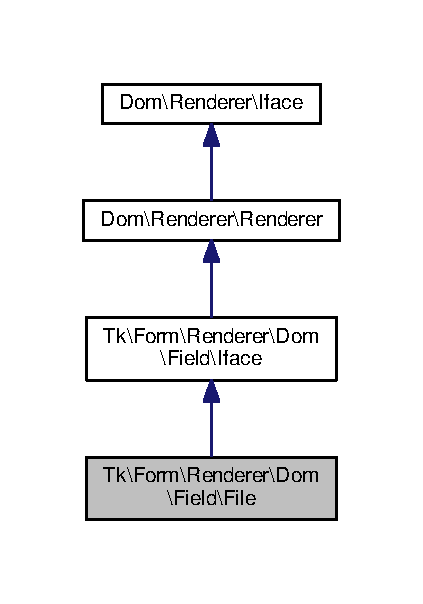
\includegraphics[width=203pt]{classTk_1_1Form_1_1Renderer_1_1Dom_1_1Field_1_1File__inherit__graph}
\end{center}
\end{figure}
\subsection*{Public Member Functions}
\begin{DoxyCompactItemize}
\item 
\hyperlink{classTk_1_1Form_1_1Renderer_1_1Dom_1_1Field_1_1File_adc2d7a4f70c408469660a243ec791acc}{show} ()
\item 
\hyperlink{classTk_1_1Form_1_1Renderer_1_1Dom_1_1Field_1_1File_a4215918ec6cfc443a79c6056e202bbfc}{show\+Element} ()
\item 
\hyperlink{classTk_1_1Form_1_1Renderer_1_1Dom_1_1Field_1_1File_a8a3d2814b6bac7136df9e0ffbc868f7a}{\+\_\+\+\_\+make\+Template} ()
\end{DoxyCompactItemize}
\subsection*{Additional Inherited Members}


\subsection{Detailed Description}
\begin{DoxyAuthor}{Author}
Michael Mifsud \href{mailto:info@tropotek.com}{\tt info@tropotek.\+com} \hyperlink{}{Copyright 2015 Michael Mifsud }
\end{DoxyAuthor}


\subsection{Member Function Documentation}
\hypertarget{classTk_1_1Form_1_1Renderer_1_1Dom_1_1Field_1_1File_a8a3d2814b6bac7136df9e0ffbc868f7a}{\index{Tk\+::\+Form\+::\+Renderer\+::\+Dom\+::\+Field\+::\+File@{Tk\+::\+Form\+::\+Renderer\+::\+Dom\+::\+Field\+::\+File}!\+\_\+\+\_\+make\+Template@{\+\_\+\+\_\+make\+Template}}
\index{\+\_\+\+\_\+make\+Template@{\+\_\+\+\_\+make\+Template}!Tk\+::\+Form\+::\+Renderer\+::\+Dom\+::\+Field\+::\+File@{Tk\+::\+Form\+::\+Renderer\+::\+Dom\+::\+Field\+::\+File}}
\subsubsection[{\+\_\+\+\_\+make\+Template}]{\setlength{\rightskip}{0pt plus 5cm}Tk\textbackslash{}\+Form\textbackslash{}\+Renderer\textbackslash{}\+Dom\textbackslash{}\+Field\textbackslash{}\+File\+::\+\_\+\+\_\+make\+Template (
\begin{DoxyParamCaption}
{}
\end{DoxyParamCaption}
)}}\label{classTk_1_1Form_1_1Renderer_1_1Dom_1_1Field_1_1File_a8a3d2814b6bac7136df9e0ffbc868f7a}
The default element template

\begin{DoxyReturn}{Returns}

\end{DoxyReturn}
\hypertarget{classTk_1_1Form_1_1Renderer_1_1Dom_1_1Field_1_1File_adc2d7a4f70c408469660a243ec791acc}{\index{Tk\+::\+Form\+::\+Renderer\+::\+Dom\+::\+Field\+::\+File@{Tk\+::\+Form\+::\+Renderer\+::\+Dom\+::\+Field\+::\+File}!show@{show}}
\index{show@{show}!Tk\+::\+Form\+::\+Renderer\+::\+Dom\+::\+Field\+::\+File@{Tk\+::\+Form\+::\+Renderer\+::\+Dom\+::\+Field\+::\+File}}
\subsubsection[{show}]{\setlength{\rightskip}{0pt plus 5cm}Tk\textbackslash{}\+Form\textbackslash{}\+Renderer\textbackslash{}\+Dom\textbackslash{}\+Field\textbackslash{}\+File\+::show (
\begin{DoxyParamCaption}
{}
\end{DoxyParamCaption}
)}}\label{classTk_1_1Form_1_1Renderer_1_1Dom_1_1Field_1_1File_adc2d7a4f70c408469660a243ec791acc}
Render the field 

Implements \hyperlink{interfaceDom_1_1Renderer_1_1Iface_a79a0ba41fb6714d69156891d6326bd33}{Dom\textbackslash{}\+Renderer\textbackslash{}\+Iface}.

\hypertarget{classTk_1_1Form_1_1Renderer_1_1Dom_1_1Field_1_1File_a4215918ec6cfc443a79c6056e202bbfc}{\index{Tk\+::\+Form\+::\+Renderer\+::\+Dom\+::\+Field\+::\+File@{Tk\+::\+Form\+::\+Renderer\+::\+Dom\+::\+Field\+::\+File}!show\+Element@{show\+Element}}
\index{show\+Element@{show\+Element}!Tk\+::\+Form\+::\+Renderer\+::\+Dom\+::\+Field\+::\+File@{Tk\+::\+Form\+::\+Renderer\+::\+Dom\+::\+Field\+::\+File}}
\subsubsection[{show\+Element}]{\setlength{\rightskip}{0pt plus 5cm}Tk\textbackslash{}\+Form\textbackslash{}\+Renderer\textbackslash{}\+Dom\textbackslash{}\+Field\textbackslash{}\+File\+::show\+Element (
\begin{DoxyParamCaption}
{}
\end{DoxyParamCaption}
)}}\label{classTk_1_1Form_1_1Renderer_1_1Dom_1_1Field_1_1File_a4215918ec6cfc443a79c6056e202bbfc}
Render the field and return the template or html string 

The documentation for this class was generated from the following file\+:\begin{DoxyCompactItemize}
\item 
vendor/ttek/tk-\/form/\+Tk/\+Form/\+Renderer/\+Dom/\+Field/File.\+php\end{DoxyCompactItemize}

\hypertarget{classTk_1_1Form_1_1Field_1_1File}{\section{Tk\textbackslash{}Form\textbackslash{}Field\textbackslash{}File Class Reference}
\label{classTk_1_1Form_1_1Field_1_1File}\index{Tk\textbackslash{}\+Form\textbackslash{}\+Field\textbackslash{}\+File@{Tk\textbackslash{}\+Form\textbackslash{}\+Field\textbackslash{}\+File}}
}


Inheritance diagram for Tk\textbackslash{}Form\textbackslash{}Field\textbackslash{}File\+:\nopagebreak
\begin{figure}[H]
\begin{center}
\leavevmode
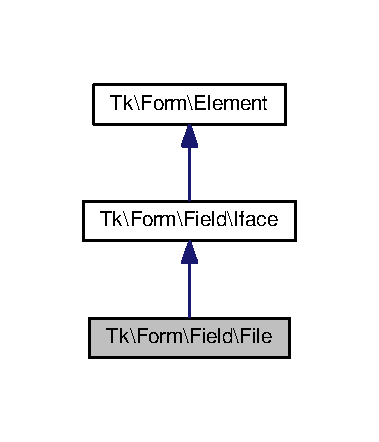
\includegraphics[width=182pt]{classTk_1_1Form_1_1Field_1_1File__inherit__graph}
\end{center}
\end{figure}
\subsection*{Public Member Functions}
\begin{DoxyCompactItemize}
\item 
\hyperlink{classTk_1_1Form_1_1Field_1_1File_a5cd6d92c83a696b8af00caaea7c7309c}{\+\_\+\+\_\+construct} (\$name)
\item 
\hyperlink{classTk_1_1Form_1_1Field_1_1File_ae2bebe9795936dd80da8df5b4aee0e7e}{set\+Form} (\hyperlink{classTk_1_1Form}{Form} \$form)
\item 
\hyperlink{classTk_1_1Form_1_1Field_1_1File_a81fd8c13f395867c42ee236309d6b72c}{get\+Max\+File\+Size} ()
\item 
\hyperlink{classTk_1_1Form_1_1Field_1_1File_a423acc6e9a9af1a99729b0cbe46db9a7}{get\+File\+Info} ()
\item 
\hyperlink{classTk_1_1Form_1_1Field_1_1File_a83ae34c5096f68cfa9ba43560e8eeb0c}{has\+File} ()
\item 
\hyperlink{classTk_1_1Form_1_1Field_1_1File_a5dd623ac92ad32223cc62152fdc5061e}{count} ()
\item 
\hyperlink{classTk_1_1Form_1_1Field_1_1File_a6fd720acaa328f48183dc66f7192113c}{is\+Valid} (\$required=false)
\item 
\hyperlink{classTk_1_1Form_1_1Field_1_1File_a60c227e20db37a2340e2eeef25e0d615}{move\+Uploaded\+File} (\$dir)
\end{DoxyCompactItemize}
\subsection*{Static Public Member Functions}
\begin{DoxyCompactItemize}
\item 
static \hyperlink{classTk_1_1Form_1_1Field_1_1File_a0ac694bd65836bc584533579364410b3}{get\+Ext} (\$filename)
\item 
static \hyperlink{classTk_1_1Form_1_1Field_1_1File_a94fda7e0599b8bda3cfc05023244c19b}{get\+Error\+String} (\$error\+Id=null)
\item 
static \hyperlink{classTk_1_1Form_1_1Field_1_1File_aeb0ac3abb4651253f31e06c0093b268c}{string2\+Bytes} (\$str)
\item 
static \hyperlink{classTk_1_1Form_1_1Field_1_1File_aadfdba00a25ea2df6d2c7568d15a8683}{bytes2\+String} (\$bytes, \$round=2)
\end{DoxyCompactItemize}
\subsection*{Protected Attributes}
\begin{DoxyCompactItemize}
\item 
\hypertarget{classTk_1_1Form_1_1Field_1_1File_a01371de48b4145e9fd6c9022a0683ee2}{{\bfseries \$max\+Bytes} = 0}\label{classTk_1_1Form_1_1Field_1_1File_a01371de48b4145e9fd6c9022a0683ee2}

\end{DoxyCompactItemize}
\subsection*{Additional Inherited Members}


\subsection{Detailed Description}
Class Text

\begin{DoxyAuthor}{Author}
Michael Mifsud \href{mailto:info@tropotek.com}{\tt info@tropotek.\+com} \hyperlink{}{Copyright 2015 Michael Mifsud }
\end{DoxyAuthor}


\subsection{Constructor \& Destructor Documentation}
\hypertarget{classTk_1_1Form_1_1Field_1_1File_a5cd6d92c83a696b8af00caaea7c7309c}{\index{Tk\+::\+Form\+::\+Field\+::\+File@{Tk\+::\+Form\+::\+Field\+::\+File}!\+\_\+\+\_\+construct@{\+\_\+\+\_\+construct}}
\index{\+\_\+\+\_\+construct@{\+\_\+\+\_\+construct}!Tk\+::\+Form\+::\+Field\+::\+File@{Tk\+::\+Form\+::\+Field\+::\+File}}
\subsubsection[{\+\_\+\+\_\+construct}]{\setlength{\rightskip}{0pt plus 5cm}Tk\textbackslash{}\+Form\textbackslash{}\+Field\textbackslash{}\+File\+::\+\_\+\+\_\+construct (
\begin{DoxyParamCaption}
\item[{}]{\$name}
\end{DoxyParamCaption}
)}}\label{classTk_1_1Form_1_1Field_1_1File_a5cd6d92c83a696b8af00caaea7c7309c}
\+\_\+\+\_\+construct


\begin{DoxyParams}[1]{Parameters}
string & {\em \$name} & \\
\hline
\end{DoxyParams}


\subsection{Member Function Documentation}
\hypertarget{classTk_1_1Form_1_1Field_1_1File_aadfdba00a25ea2df6d2c7568d15a8683}{\index{Tk\+::\+Form\+::\+Field\+::\+File@{Tk\+::\+Form\+::\+Field\+::\+File}!bytes2\+String@{bytes2\+String}}
\index{bytes2\+String@{bytes2\+String}!Tk\+::\+Form\+::\+Field\+::\+File@{Tk\+::\+Form\+::\+Field\+::\+File}}
\subsubsection[{bytes2\+String}]{\setlength{\rightskip}{0pt plus 5cm}static Tk\textbackslash{}\+Form\textbackslash{}\+Field\textbackslash{}\+File\+::bytes2\+String (
\begin{DoxyParamCaption}
\item[{}]{\$bytes, }
\item[{}]{\$round = {\ttfamily 2}}
\end{DoxyParamCaption}
)\hspace{0.3cm}{\ttfamily [static]}}}\label{classTk_1_1Form_1_1Field_1_1File_aadfdba00a25ea2df6d2c7568d15a8683}
Convert a value from bytes to a human readable value


\begin{DoxyParams}[1]{Parameters}
int & {\em \$bytes} & \\
\hline
\end{DoxyParams}
\begin{DoxyReturn}{Returns}
string 
\end{DoxyReturn}
\begin{DoxyAuthor}{Author}
\href{http://php-pdb.sourceforge.net/samples/viewSource.php?file=twister.php}{\tt http\+://php-\/pdb.\+sourceforge.\+net/samples/view\+Source.\+php?file=twister.\+php} 
\end{DoxyAuthor}
\hypertarget{classTk_1_1Form_1_1Field_1_1File_a5dd623ac92ad32223cc62152fdc5061e}{\index{Tk\+::\+Form\+::\+Field\+::\+File@{Tk\+::\+Form\+::\+Field\+::\+File}!count@{count}}
\index{count@{count}!Tk\+::\+Form\+::\+Field\+::\+File@{Tk\+::\+Form\+::\+Field\+::\+File}}
\subsubsection[{count}]{\setlength{\rightskip}{0pt plus 5cm}Tk\textbackslash{}\+Form\textbackslash{}\+Field\textbackslash{}\+File\+::count (
\begin{DoxyParamCaption}
{}
\end{DoxyParamCaption}
)}}\label{classTk_1_1Form_1_1Field_1_1File_a5dd623ac92ad32223cc62152fdc5061e}
Has there been a file submitted?

return boolean \hypertarget{classTk_1_1Form_1_1Field_1_1File_a94fda7e0599b8bda3cfc05023244c19b}{\index{Tk\+::\+Form\+::\+Field\+::\+File@{Tk\+::\+Form\+::\+Field\+::\+File}!get\+Error\+String@{get\+Error\+String}}
\index{get\+Error\+String@{get\+Error\+String}!Tk\+::\+Form\+::\+Field\+::\+File@{Tk\+::\+Form\+::\+Field\+::\+File}}
\subsubsection[{get\+Error\+String}]{\setlength{\rightskip}{0pt plus 5cm}static Tk\textbackslash{}\+Form\textbackslash{}\+Field\textbackslash{}\+File\+::get\+Error\+String (
\begin{DoxyParamCaption}
\item[{}]{\$error\+Id = {\ttfamily null}}
\end{DoxyParamCaption}
)\hspace{0.3cm}{\ttfamily [static]}}}\label{classTk_1_1Form_1_1Field_1_1File_a94fda7e0599b8bda3cfc05023244c19b}
get\+Error\+String


\begin{DoxyParams}[1]{Parameters}
int & {\em \$error\+Id} & \\
\hline
\end{DoxyParams}
\begin{DoxyReturn}{Returns}
string 
\end{DoxyReturn}
\hypertarget{classTk_1_1Form_1_1Field_1_1File_a0ac694bd65836bc584533579364410b3}{\index{Tk\+::\+Form\+::\+Field\+::\+File@{Tk\+::\+Form\+::\+Field\+::\+File}!get\+Ext@{get\+Ext}}
\index{get\+Ext@{get\+Ext}!Tk\+::\+Form\+::\+Field\+::\+File@{Tk\+::\+Form\+::\+Field\+::\+File}}
\subsubsection[{get\+Ext}]{\setlength{\rightskip}{0pt plus 5cm}static Tk\textbackslash{}\+Form\textbackslash{}\+Field\textbackslash{}\+File\+::get\+Ext (
\begin{DoxyParamCaption}
\item[{}]{\$filename}
\end{DoxyParamCaption}
)\hspace{0.3cm}{\ttfamily [static]}}}\label{classTk_1_1Form_1_1Field_1_1File_a0ac694bd65836bc584533579364410b3}
Get the uploaded filename, will return empty string if no file exists The original name of the file on the client machine.

\begin{DoxyReturn}{Returns}
string 
\end{DoxyReturn}
\hypertarget{classTk_1_1Form_1_1Field_1_1File_a423acc6e9a9af1a99729b0cbe46db9a7}{\index{Tk\+::\+Form\+::\+Field\+::\+File@{Tk\+::\+Form\+::\+Field\+::\+File}!get\+File\+Info@{get\+File\+Info}}
\index{get\+File\+Info@{get\+File\+Info}!Tk\+::\+Form\+::\+Field\+::\+File@{Tk\+::\+Form\+::\+Field\+::\+File}}
\subsubsection[{get\+File\+Info}]{\setlength{\rightskip}{0pt plus 5cm}Tk\textbackslash{}\+Form\textbackslash{}\+Field\textbackslash{}\+File\+::get\+File\+Info (
\begin{DoxyParamCaption}
{}
\end{DoxyParamCaption}
)}}\label{classTk_1_1Form_1_1Field_1_1File_a423acc6e9a9af1a99729b0cbe46db9a7}
Returns the file\+Info array or if null it will try to lookup the \$\+\_\+\+F\+I\+L\+E\+S\mbox{[}\$field\+Name\mbox{]} array for the file\+Info If it exists it will set the instance parameter of File\+Info to this array.

\begin{DoxyReturn}{Returns}
array 
\end{DoxyReturn}
\hypertarget{classTk_1_1Form_1_1Field_1_1File_a81fd8c13f395867c42ee236309d6b72c}{\index{Tk\+::\+Form\+::\+Field\+::\+File@{Tk\+::\+Form\+::\+Field\+::\+File}!get\+Max\+File\+Size@{get\+Max\+File\+Size}}
\index{get\+Max\+File\+Size@{get\+Max\+File\+Size}!Tk\+::\+Form\+::\+Field\+::\+File@{Tk\+::\+Form\+::\+Field\+::\+File}}
\subsubsection[{get\+Max\+File\+Size}]{\setlength{\rightskip}{0pt plus 5cm}Tk\textbackslash{}\+Form\textbackslash{}\+Field\textbackslash{}\+File\+::get\+Max\+File\+Size (
\begin{DoxyParamCaption}
{}
\end{DoxyParamCaption}
)}}\label{classTk_1_1Form_1_1Field_1_1File_a81fd8c13f395867c42ee236309d6b72c}
Get the max filesize in bytes for this file field

\begin{DoxyReturn}{Returns}
int 
\end{DoxyReturn}
\hypertarget{classTk_1_1Form_1_1Field_1_1File_a83ae34c5096f68cfa9ba43560e8eeb0c}{\index{Tk\+::\+Form\+::\+Field\+::\+File@{Tk\+::\+Form\+::\+Field\+::\+File}!has\+File@{has\+File}}
\index{has\+File@{has\+File}!Tk\+::\+Form\+::\+Field\+::\+File@{Tk\+::\+Form\+::\+Field\+::\+File}}
\subsubsection[{has\+File}]{\setlength{\rightskip}{0pt plus 5cm}Tk\textbackslash{}\+Form\textbackslash{}\+Field\textbackslash{}\+File\+::has\+File (
\begin{DoxyParamCaption}
{}
\end{DoxyParamCaption}
)}}\label{classTk_1_1Form_1_1Field_1_1File_a83ae34c5096f68cfa9ba43560e8eeb0c}
Has there been a file submitted?

return boolean \hypertarget{classTk_1_1Form_1_1Field_1_1File_a6fd720acaa328f48183dc66f7192113c}{\index{Tk\+::\+Form\+::\+Field\+::\+File@{Tk\+::\+Form\+::\+Field\+::\+File}!is\+Valid@{is\+Valid}}
\index{is\+Valid@{is\+Valid}!Tk\+::\+Form\+::\+Field\+::\+File@{Tk\+::\+Form\+::\+Field\+::\+File}}
\subsubsection[{is\+Valid}]{\setlength{\rightskip}{0pt plus 5cm}Tk\textbackslash{}\+Form\textbackslash{}\+Field\textbackslash{}\+File\+::is\+Valid (
\begin{DoxyParamCaption}
\item[{}]{\$required = {\ttfamily false}}
\end{DoxyParamCaption}
)}}\label{classTk_1_1Form_1_1Field_1_1File_a6fd720acaa328f48183dc66f7192113c}
validate the uploaded file

\begin{DoxyReturn}{Returns}
bool 
\end{DoxyReturn}
\hypertarget{classTk_1_1Form_1_1Field_1_1File_a60c227e20db37a2340e2eeef25e0d615}{\index{Tk\+::\+Form\+::\+Field\+::\+File@{Tk\+::\+Form\+::\+Field\+::\+File}!move\+Uploaded\+File@{move\+Uploaded\+File}}
\index{move\+Uploaded\+File@{move\+Uploaded\+File}!Tk\+::\+Form\+::\+Field\+::\+File@{Tk\+::\+Form\+::\+Field\+::\+File}}
\subsubsection[{move\+Uploaded\+File}]{\setlength{\rightskip}{0pt plus 5cm}Tk\textbackslash{}\+Form\textbackslash{}\+Field\textbackslash{}\+File\+::move\+Uploaded\+File (
\begin{DoxyParamCaption}
\item[{}]{\$dir}
\end{DoxyParamCaption}
)}}\label{classTk_1_1Form_1_1Field_1_1File_a60c227e20db37a2340e2eeef25e0d615}
Use this to move the attached files to the directory in \$dir

If the directory does not exist it will try to create it for you.

You may still use the move\+\_\+uploaded\+\_\+file() function standalone if you prefer to have control of the saved filenames


\begin{DoxyParams}[1]{Parameters}
string & {\em \$dir} & \\
\hline
\end{DoxyParams}
\begin{DoxyReturn}{Returns}
bool 
\end{DoxyReturn}
\hypertarget{classTk_1_1Form_1_1Field_1_1File_ae2bebe9795936dd80da8df5b4aee0e7e}{\index{Tk\+::\+Form\+::\+Field\+::\+File@{Tk\+::\+Form\+::\+Field\+::\+File}!set\+Form@{set\+Form}}
\index{set\+Form@{set\+Form}!Tk\+::\+Form\+::\+Field\+::\+File@{Tk\+::\+Form\+::\+Field\+::\+File}}
\subsubsection[{set\+Form}]{\setlength{\rightskip}{0pt plus 5cm}Tk\textbackslash{}\+Form\textbackslash{}\+Field\textbackslash{}\+File\+::set\+Form (
\begin{DoxyParamCaption}
\item[{{\bf Form}}]{\$form}
\end{DoxyParamCaption}
)}}\label{classTk_1_1Form_1_1Field_1_1File_ae2bebe9795936dd80da8df5b4aee0e7e}
Set the form for this element


\begin{DoxyParams}[1]{Parameters}
\hyperlink{classTk_1_1Form}{Form} & {\em \$form} & \\
\hline
\end{DoxyParams}
\begin{DoxyReturn}{Returns}
\$this 
\end{DoxyReturn}
\hypertarget{classTk_1_1Form_1_1Field_1_1File_aeb0ac3abb4651253f31e06c0093b268c}{\index{Tk\+::\+Form\+::\+Field\+::\+File@{Tk\+::\+Form\+::\+Field\+::\+File}!string2\+Bytes@{string2\+Bytes}}
\index{string2\+Bytes@{string2\+Bytes}!Tk\+::\+Form\+::\+Field\+::\+File@{Tk\+::\+Form\+::\+Field\+::\+File}}
\subsubsection[{string2\+Bytes}]{\setlength{\rightskip}{0pt plus 5cm}static Tk\textbackslash{}\+Form\textbackslash{}\+Field\textbackslash{}\+File\+::string2\+Bytes (
\begin{DoxyParamCaption}
\item[{}]{\$str}
\end{DoxyParamCaption}
)\hspace{0.3cm}{\ttfamily [static]}}}\label{classTk_1_1Form_1_1Field_1_1File_aeb0ac3abb4651253f31e06c0093b268c}
Get the bytes from a string like 40\+M, 10\+T, 100\+K


\begin{DoxyParams}[1]{Parameters}
string & {\em \$str} & \\
\hline
\end{DoxyParams}
\begin{DoxyReturn}{Returns}
int 
\end{DoxyReturn}


The documentation for this class was generated from the following file\+:\begin{DoxyCompactItemize}
\item 
vendor/ttek/tk-\/form/\+Tk/\+Form/\+Field/File.\+php\end{DoxyCompactItemize}

\hypertarget{classTk_1_1Form_1_1Renderer_1_1Dom_1_1Form}{\section{Tk\textbackslash{}Form\textbackslash{}Renderer\textbackslash{}Dom\textbackslash{}Form Class Reference}
\label{classTk_1_1Form_1_1Renderer_1_1Dom_1_1Form}\index{Tk\textbackslash{}\+Form\textbackslash{}\+Renderer\textbackslash{}\+Dom\textbackslash{}\+Form@{Tk\textbackslash{}\+Form\textbackslash{}\+Renderer\textbackslash{}\+Dom\textbackslash{}\+Form}}
}


Inheritance diagram for Tk\textbackslash{}Form\textbackslash{}Renderer\textbackslash{}Dom\textbackslash{}Form\+:\nopagebreak
\begin{figure}[H]
\begin{center}
\leavevmode
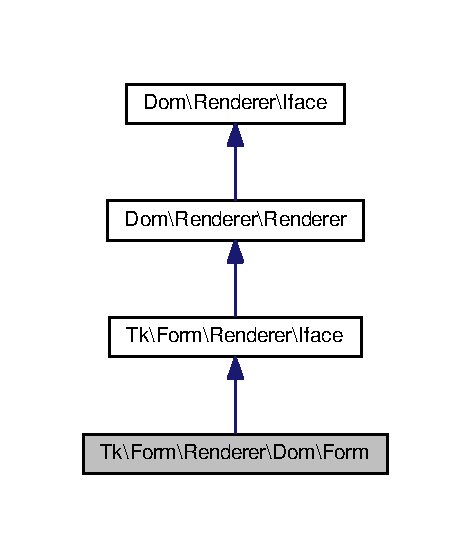
\includegraphics[width=226pt]{classTk_1_1Form_1_1Renderer_1_1Dom_1_1Form__inherit__graph}
\end{center}
\end{figure}
\subsection*{Public Member Functions}
\begin{DoxyCompactItemize}
\item 
\hyperlink{classTk_1_1Form_1_1Renderer_1_1Dom_1_1Form_a2b67b6b33d1cffdffc04010dad181b93}{show} ()
\item 
\hyperlink{classTk_1_1Form_1_1Renderer_1_1Dom_1_1Form_a5897b87d63f146172fa962206bcb38bf}{\+\_\+\+\_\+make\+Template} ()
\end{DoxyCompactItemize}
\subsection*{Static Public Member Functions}
\begin{DoxyCompactItemize}
\item 
static \hyperlink{classTk_1_1Form_1_1Renderer_1_1Dom_1_1Form_af2be34b469d7433b657390e259d6e634}{create} (\$form)
\end{DoxyCompactItemize}
\subsection*{Protected Member Functions}
\begin{DoxyCompactItemize}
\item 
\hyperlink{classTk_1_1Form_1_1Renderer_1_1Dom_1_1Form_ad899e315239e56d0365cf002bb2a1621}{show\+Field} (\hyperlink{classTk_1_1Form_1_1Renderer_1_1Dom_1_1Field_1_1Iface}{Field\textbackslash{}\+Iface} \$field)
\end{DoxyCompactItemize}
\subsection*{Additional Inherited Members}


\subsection{Detailed Description}
A Dom Renderer for the form object

\begin{DoxyAuthor}{Author}
Michael Mifsud \href{mailto:info@tropotek.com}{\tt info@tropotek.\+com} \hyperlink{}{Copyright 2015 Michael Mifsud }
\end{DoxyAuthor}


\subsection{Member Function Documentation}
\hypertarget{classTk_1_1Form_1_1Renderer_1_1Dom_1_1Form_a5897b87d63f146172fa962206bcb38bf}{\index{Tk\+::\+Form\+::\+Renderer\+::\+Dom\+::\+Form@{Tk\+::\+Form\+::\+Renderer\+::\+Dom\+::\+Form}!\+\_\+\+\_\+make\+Template@{\+\_\+\+\_\+make\+Template}}
\index{\+\_\+\+\_\+make\+Template@{\+\_\+\+\_\+make\+Template}!Tk\+::\+Form\+::\+Renderer\+::\+Dom\+::\+Form@{Tk\+::\+Form\+::\+Renderer\+::\+Dom\+::\+Form}}
\subsubsection[{\+\_\+\+\_\+make\+Template}]{\setlength{\rightskip}{0pt plus 5cm}Tk\textbackslash{}\+Form\textbackslash{}\+Renderer\textbackslash{}\+Dom\textbackslash{}\+Form\+::\+\_\+\+\_\+make\+Template (
\begin{DoxyParamCaption}
{}
\end{DoxyParamCaption}
)}}\label{classTk_1_1Form_1_1Renderer_1_1Dom_1_1Form_a5897b87d63f146172fa962206bcb38bf}
make\+Template

\begin{DoxyReturn}{Returns}
string 
\end{DoxyReturn}
\hypertarget{classTk_1_1Form_1_1Renderer_1_1Dom_1_1Form_af2be34b469d7433b657390e259d6e634}{\index{Tk\+::\+Form\+::\+Renderer\+::\+Dom\+::\+Form@{Tk\+::\+Form\+::\+Renderer\+::\+Dom\+::\+Form}!create@{create}}
\index{create@{create}!Tk\+::\+Form\+::\+Renderer\+::\+Dom\+::\+Form@{Tk\+::\+Form\+::\+Renderer\+::\+Dom\+::\+Form}}
\subsubsection[{create}]{\setlength{\rightskip}{0pt plus 5cm}static Tk\textbackslash{}\+Form\textbackslash{}\+Renderer\textbackslash{}\+Dom\textbackslash{}\+Form\+::create (
\begin{DoxyParamCaption}
\item[{}]{\$form}
\end{DoxyParamCaption}
)\hspace{0.3cm}{\ttfamily [static]}}}\label{classTk_1_1Form_1_1Renderer_1_1Dom_1_1Form_af2be34b469d7433b657390e259d6e634}
Create a new Renderer.


\begin{DoxyParams}[1]{Parameters}
\textbackslash{}\+Tk\textbackslash{}\+Form & {\em \$form} & \\
\hline
\end{DoxyParams}
\begin{DoxyReturn}{Returns}
\hyperlink{classTk_1_1Form_1_1Renderer_1_1Dom_1_1Form}{Form} 
\end{DoxyReturn}
\hypertarget{classTk_1_1Form_1_1Renderer_1_1Dom_1_1Form_a2b67b6b33d1cffdffc04010dad181b93}{\index{Tk\+::\+Form\+::\+Renderer\+::\+Dom\+::\+Form@{Tk\+::\+Form\+::\+Renderer\+::\+Dom\+::\+Form}!show@{show}}
\index{show@{show}!Tk\+::\+Form\+::\+Renderer\+::\+Dom\+::\+Form@{Tk\+::\+Form\+::\+Renderer\+::\+Dom\+::\+Form}}
\subsubsection[{show}]{\setlength{\rightskip}{0pt plus 5cm}Tk\textbackslash{}\+Form\textbackslash{}\+Renderer\textbackslash{}\+Dom\textbackslash{}\+Form\+::show (
\begin{DoxyParamCaption}
{}
\end{DoxyParamCaption}
)}}\label{classTk_1_1Form_1_1Renderer_1_1Dom_1_1Form_a2b67b6b33d1cffdffc04010dad181b93}
Render the field and return the template or html string

\begin{DoxyReturn}{Returns}
mixed 
\end{DoxyReturn}


Implements \hyperlink{interfaceDom_1_1Renderer_1_1Iface_a79a0ba41fb6714d69156891d6326bd33}{Dom\textbackslash{}\+Renderer\textbackslash{}\+Iface}.

\hypertarget{classTk_1_1Form_1_1Renderer_1_1Dom_1_1Form_ad899e315239e56d0365cf002bb2a1621}{\index{Tk\+::\+Form\+::\+Renderer\+::\+Dom\+::\+Form@{Tk\+::\+Form\+::\+Renderer\+::\+Dom\+::\+Form}!show\+Field@{show\+Field}}
\index{show\+Field@{show\+Field}!Tk\+::\+Form\+::\+Renderer\+::\+Dom\+::\+Form@{Tk\+::\+Form\+::\+Renderer\+::\+Dom\+::\+Form}}
\subsubsection[{show\+Field}]{\setlength{\rightskip}{0pt plus 5cm}Tk\textbackslash{}\+Form\textbackslash{}\+Renderer\textbackslash{}\+Dom\textbackslash{}\+Form\+::show\+Field (
\begin{DoxyParamCaption}
\item[{{\bf Field\textbackslash{}\+Iface}}]{\$field}
\end{DoxyParamCaption}
)\hspace{0.3cm}{\ttfamily [protected]}}}\label{classTk_1_1Form_1_1Renderer_1_1Dom_1_1Form_ad899e315239e56d0365cf002bb2a1621}
Render Fields


\begin{DoxyParams}[1]{Parameters}
Field\textbackslash{}\+Iface & {\em \$field} & \\
\hline
\end{DoxyParams}
\begin{DoxyReturn}{Returns}
mixed 
\end{DoxyReturn}


The documentation for this class was generated from the following file\+:\begin{DoxyCompactItemize}
\item 
vendor/ttek/tk-\/form/\+Tk/\+Form/\+Renderer/\+Dom/Form.\+php\end{DoxyCompactItemize}

\hypertarget{classDom_1_1Form}{\section{Dom\textbackslash{}Form Class Reference}
\label{classDom_1_1Form}\index{Dom\textbackslash{}\+Form@{Dom\textbackslash{}\+Form}}
}
\subsection*{Public Member Functions}
\begin{DoxyCompactItemize}
\item 
\hyperlink{classDom_1_1Form_a65e0888bc892af6518bef66f4478493f}{\+\_\+\+\_\+construct} (\$form, \$elements, \$parent)
\item 
\hyperlink{classDom_1_1Form_a6a3f04acb0a15057b191288856e32988}{is\+Submitted} ()
\item 
\hyperlink{classDom_1_1Form_a7dcc534e1500c9cbb1917b94960725b7}{get\+Form\+Element} (\$name, \$i=0)
\item 
\hyperlink{classDom_1_1Form_a26a92a24ca4f392489a362d4dd7c832b}{get\+Form\+Element\+List} (\$name)
\item 
\hyperlink{classDom_1_1Form_aae8f3dfcb80c15e2d146d69284d4bf21}{get\+Num\+Form\+Elements} (\$name)
\item 
\hyperlink{classDom_1_1Form_a012cd2a2f66f327b0d612cee92c0f0d7}{form\+Element\+Exists} (\$key)
\item 
\hyperlink{classDom_1_1Form_a025318e2647c2104a05c988dd60375bc}{get\+Element\+Names} ()
\item 
\hyperlink{classDom_1_1Form_aa753a68f4a318cee9ff7597789b257a5}{set\+Action} (\$value)
\item 
\hyperlink{classDom_1_1Form_a57fa48ce5b5698514510998a348ed0ba}{set\+Method} (\$value)
\item 
\hyperlink{classDom_1_1Form_aae7371f8752cd97d1d4f5e58c5c0a6b2}{set\+Target} (\$value)
\item 
\hyperlink{classDom_1_1Form_a6da827a320f7f556ec1fc5bc75fbfa86}{append\+Hidden\+Element} (\$name, \$value)
\item 
\hyperlink{classDom_1_1Form_a8a96c65e40603aab1bc2342363a252e9}{get\+Name} ()
\item 
\hyperlink{classDom_1_1Form_a2d10dcb8fba24faacbe7f64ed2b9da47}{get\+Id} ()
\item 
\hyperlink{classDom_1_1Form_a6765bb1f7b8060355440c98c433731d7}{get\+Node} ()
\item 
\hyperlink{classDom_1_1Form_a5435b6a3041204ce9825a1c5e00c58a7}{get\+Template} ()
\end{DoxyCompactItemize}
\subsection*{Protected Attributes}
\begin{DoxyCompactItemize}
\item 
\hypertarget{classDom_1_1Form_ad9af9661b262865f693047ca95a75dfc}{{\bfseries \$form} = null}\label{classDom_1_1Form_ad9af9661b262865f693047ca95a75dfc}

\item 
\hypertarget{classDom_1_1Form_ad9fad3d4e275ddbe500c88de63259256}{{\bfseries \$elements} = array()}\label{classDom_1_1Form_ad9fad3d4e275ddbe500c88de63259256}

\item 
\hypertarget{classDom_1_1Form_a036af1b6687a64ec98970ea627947162}{{\bfseries \$parent} = null}\label{classDom_1_1Form_a036af1b6687a64ec98970ea627947162}

\end{DoxyCompactItemize}


\subsection{Detailed Description}
The form package make an A\+P\+I available for rendering a form and its elements

The form package currently does not fully support element arrays. It can be done but it is not fully supported or tested.

\begin{DoxyAuthor}{Author}
Michael Mifsud 

Darryl Ross \hyperlink{}{Copyright 2007 }
\end{DoxyAuthor}


\subsection{Constructor \& Destructor Documentation}
\hypertarget{classDom_1_1Form_a65e0888bc892af6518bef66f4478493f}{\index{Dom\+::\+Form@{Dom\+::\+Form}!\+\_\+\+\_\+construct@{\+\_\+\+\_\+construct}}
\index{\+\_\+\+\_\+construct@{\+\_\+\+\_\+construct}!Dom\+::\+Form@{Dom\+::\+Form}}
\subsubsection[{\+\_\+\+\_\+construct}]{\setlength{\rightskip}{0pt plus 5cm}Dom\textbackslash{}\+Form\+::\+\_\+\+\_\+construct (
\begin{DoxyParamCaption}
\item[{}]{\$form, }
\item[{}]{\$elements, }
\item[{}]{\$parent}
\end{DoxyParamCaption}
)}}\label{classDom_1_1Form_a65e0888bc892af6518bef66f4478493f}
\+\_\+\+\_\+construct


\begin{DoxyParams}[1]{Parameters}
\textbackslash{}\+D\+O\+M\+Element & {\em \$form} & \\
\hline
array & {\em \$elements} & An array of form elements \\
\hline
\hyperlink{classDom_1_1Template}{Template} & {\em \$parent} & The parent object \\
\hline
\end{DoxyParams}


\subsection{Member Function Documentation}
\hypertarget{classDom_1_1Form_a6da827a320f7f556ec1fc5bc75fbfa86}{\index{Dom\+::\+Form@{Dom\+::\+Form}!append\+Hidden\+Element@{append\+Hidden\+Element}}
\index{append\+Hidden\+Element@{append\+Hidden\+Element}!Dom\+::\+Form@{Dom\+::\+Form}}
\subsubsection[{append\+Hidden\+Element}]{\setlength{\rightskip}{0pt plus 5cm}Dom\textbackslash{}\+Form\+::append\+Hidden\+Element (
\begin{DoxyParamCaption}
\item[{}]{\$name, }
\item[{}]{\$value}
\end{DoxyParamCaption}
)}}\label{classDom_1_1Form_a6da827a320f7f556ec1fc5bc75fbfa86}
Append a hidden element to a form.


\begin{DoxyParams}[1]{Parameters}
string & {\em \$name} & \\
\hline
string & {\em \$value} & \\
\hline
\end{DoxyParams}
\begin{DoxyReturn}{Returns}

\end{DoxyReturn}
\hypertarget{classDom_1_1Form_a012cd2a2f66f327b0d612cee92c0f0d7}{\index{Dom\+::\+Form@{Dom\+::\+Form}!form\+Element\+Exists@{form\+Element\+Exists}}
\index{form\+Element\+Exists@{form\+Element\+Exists}!Dom\+::\+Form@{Dom\+::\+Form}}
\subsubsection[{form\+Element\+Exists}]{\setlength{\rightskip}{0pt plus 5cm}Dom\textbackslash{}\+Form\+::form\+Element\+Exists (
\begin{DoxyParamCaption}
\item[{}]{\$key}
\end{DoxyParamCaption}
)}}\label{classDom_1_1Form_a012cd2a2f66f327b0d612cee92c0f0d7}
Check if a repeat,choice,var,form (template property) exists.


\begin{DoxyParams}[1]{Parameters}
string & {\em \$key} & \\
\hline
\end{DoxyParams}
\begin{DoxyReturn}{Returns}
bool 
\end{DoxyReturn}
\hypertarget{classDom_1_1Form_a025318e2647c2104a05c988dd60375bc}{\index{Dom\+::\+Form@{Dom\+::\+Form}!get\+Element\+Names@{get\+Element\+Names}}
\index{get\+Element\+Names@{get\+Element\+Names}!Dom\+::\+Form@{Dom\+::\+Form}}
\subsubsection[{get\+Element\+Names}]{\setlength{\rightskip}{0pt plus 5cm}Dom\textbackslash{}\+Form\+::get\+Element\+Names (
\begin{DoxyParamCaption}
{}
\end{DoxyParamCaption}
)}}\label{classDom_1_1Form_a025318e2647c2104a05c988dd60375bc}
Get an array containing the form element names

\begin{DoxyReturn}{Returns}
array 
\end{DoxyReturn}
\hypertarget{classDom_1_1Form_a7dcc534e1500c9cbb1917b94960725b7}{\index{Dom\+::\+Form@{Dom\+::\+Form}!get\+Form\+Element@{get\+Form\+Element}}
\index{get\+Form\+Element@{get\+Form\+Element}!Dom\+::\+Form@{Dom\+::\+Form}}
\subsubsection[{get\+Form\+Element}]{\setlength{\rightskip}{0pt plus 5cm}Dom\textbackslash{}\+Form\+::get\+Form\+Element (
\begin{DoxyParamCaption}
\item[{}]{\$name, }
\item[{}]{\$i = {\ttfamily 0}}
\end{DoxyParamCaption}
)}}\label{classDom_1_1Form_a7dcc534e1500c9cbb1917b94960725b7}
Return the form element with the name.


\begin{DoxyParams}[1]{Parameters}
string & {\em \$name} & \\
\hline
int & {\em \$i} & (optional) index for multiple elements \\
\hline
\end{DoxyParams}
\begin{DoxyReturn}{Returns}
\hyperlink{classDom_1_1Form_1_1Element}{Element} 
\end{DoxyReturn}
\hypertarget{classDom_1_1Form_a26a92a24ca4f392489a362d4dd7c832b}{\index{Dom\+::\+Form@{Dom\+::\+Form}!get\+Form\+Element\+List@{get\+Form\+Element\+List}}
\index{get\+Form\+Element\+List@{get\+Form\+Element\+List}!Dom\+::\+Form@{Dom\+::\+Form}}
\subsubsection[{get\+Form\+Element\+List}]{\setlength{\rightskip}{0pt plus 5cm}Dom\textbackslash{}\+Form\+::get\+Form\+Element\+List (
\begin{DoxyParamCaption}
\item[{}]{\$name}
\end{DoxyParamCaption}
)}}\label{classDom_1_1Form_a26a92a24ca4f392489a362d4dd7c832b}
Get an array of form elements with the name value Used for radio boxes and multi select lists


\begin{DoxyParams}[1]{Parameters}
string & {\em \$name} & \\
\hline
\end{DoxyParams}
\begin{DoxyReturn}{Returns}
array 
\end{DoxyReturn}
\hypertarget{classDom_1_1Form_a2d10dcb8fba24faacbe7f64ed2b9da47}{\index{Dom\+::\+Form@{Dom\+::\+Form}!get\+Id@{get\+Id}}
\index{get\+Id@{get\+Id}!Dom\+::\+Form@{Dom\+::\+Form}}
\subsubsection[{get\+Id}]{\setlength{\rightskip}{0pt plus 5cm}Dom\textbackslash{}\+Form\+::get\+Id (
\begin{DoxyParamCaption}
{}
\end{DoxyParamCaption}
)}}\label{classDom_1_1Form_a2d10dcb8fba24faacbe7f64ed2b9da47}
Get the form id attribute

\begin{DoxyReturn}{Returns}
string 
\end{DoxyReturn}
\hypertarget{classDom_1_1Form_a8a96c65e40603aab1bc2342363a252e9}{\index{Dom\+::\+Form@{Dom\+::\+Form}!get\+Name@{get\+Name}}
\index{get\+Name@{get\+Name}!Dom\+::\+Form@{Dom\+::\+Form}}
\subsubsection[{get\+Name}]{\setlength{\rightskip}{0pt plus 5cm}Dom\textbackslash{}\+Form\+::get\+Name (
\begin{DoxyParamCaption}
{}
\end{DoxyParamCaption}
)}}\label{classDom_1_1Form_a8a96c65e40603aab1bc2342363a252e9}
Get the form Name Attribute.

\begin{DoxyReturn}{Returns}
string 
\end{DoxyReturn}
\hypertarget{classDom_1_1Form_a6765bb1f7b8060355440c98c433731d7}{\index{Dom\+::\+Form@{Dom\+::\+Form}!get\+Node@{get\+Node}}
\index{get\+Node@{get\+Node}!Dom\+::\+Form@{Dom\+::\+Form}}
\subsubsection[{get\+Node}]{\setlength{\rightskip}{0pt plus 5cm}Dom\textbackslash{}\+Form\+::get\+Node (
\begin{DoxyParamCaption}
{}
\end{DoxyParamCaption}
)}}\label{classDom_1_1Form_a6765bb1f7b8060355440c98c433731d7}
Get the  of this form object.

\begin{DoxyReturn}{Returns}

\end{DoxyReturn}
\hypertarget{classDom_1_1Form_aae8f3dfcb80c15e2d146d69284d4bf21}{\index{Dom\+::\+Form@{Dom\+::\+Form}!get\+Num\+Form\+Elements@{get\+Num\+Form\+Elements}}
\index{get\+Num\+Form\+Elements@{get\+Num\+Form\+Elements}!Dom\+::\+Form@{Dom\+::\+Form}}
\subsubsection[{get\+Num\+Form\+Elements}]{\setlength{\rightskip}{0pt plus 5cm}Dom\textbackslash{}\+Form\+::get\+Num\+Form\+Elements (
\begin{DoxyParamCaption}
\item[{}]{\$name}
\end{DoxyParamCaption}
)}}\label{classDom_1_1Form_aae8f3dfcb80c15e2d146d69284d4bf21}
Return the number of elements in an element namespace


\begin{DoxyParams}[1]{Parameters}
string & {\em \$name} & \\
\hline
\end{DoxyParams}
\begin{DoxyReturn}{Returns}
int 
\end{DoxyReturn}
\hypertarget{classDom_1_1Form_a5435b6a3041204ce9825a1c5e00c58a7}{\index{Dom\+::\+Form@{Dom\+::\+Form}!get\+Template@{get\+Template}}
\index{get\+Template@{get\+Template}!Dom\+::\+Form@{Dom\+::\+Form}}
\subsubsection[{get\+Template}]{\setlength{\rightskip}{0pt plus 5cm}Dom\textbackslash{}\+Form\+::get\+Template (
\begin{DoxyParamCaption}
{}
\end{DoxyParamCaption}
)}}\label{classDom_1_1Form_a5435b6a3041204ce9825a1c5e00c58a7}
Get the parent template for this form

\begin{DoxyReturn}{Returns}
\hyperlink{classDom_1_1Template}{Template} 
\end{DoxyReturn}
\hypertarget{classDom_1_1Form_a6a3f04acb0a15057b191288856e32988}{\index{Dom\+::\+Form@{Dom\+::\+Form}!is\+Submitted@{is\+Submitted}}
\index{is\+Submitted@{is\+Submitted}!Dom\+::\+Form@{Dom\+::\+Form}}
\subsubsection[{is\+Submitted}]{\setlength{\rightskip}{0pt plus 5cm}Dom\textbackslash{}\+Form\+::is\+Submitted (
\begin{DoxyParamCaption}
{}
\end{DoxyParamCaption}
)}}\label{classDom_1_1Form_a6a3f04acb0a15057b191288856e32988}
Has the form been submitted

\begin{DoxyReturn}{Returns}
bool 
\end{DoxyReturn}
\hypertarget{classDom_1_1Form_aa753a68f4a318cee9ff7597789b257a5}{\index{Dom\+::\+Form@{Dom\+::\+Form}!set\+Action@{set\+Action}}
\index{set\+Action@{set\+Action}!Dom\+::\+Form@{Dom\+::\+Form}}
\subsubsection[{set\+Action}]{\setlength{\rightskip}{0pt plus 5cm}Dom\textbackslash{}\+Form\+::set\+Action (
\begin{DoxyParamCaption}
\item[{}]{\$value}
\end{DoxyParamCaption}
)}}\label{classDom_1_1Form_aa753a68f4a318cee9ff7597789b257a5}
Set a U\+R\+L that defines where to send the data when the submit button is pushed.


\begin{DoxyParams}[1]{Parameters}
string & {\em \$value} & \\
\hline
\end{DoxyParams}
\begin{DoxyReturn}{Returns}
\$this 
\end{DoxyReturn}
\hypertarget{classDom_1_1Form_a57fa48ce5b5698514510998a348ed0ba}{\index{Dom\+::\+Form@{Dom\+::\+Form}!set\+Method@{set\+Method}}
\index{set\+Method@{set\+Method}!Dom\+::\+Form@{Dom\+::\+Form}}
\subsubsection[{set\+Method}]{\setlength{\rightskip}{0pt plus 5cm}Dom\textbackslash{}\+Form\+::set\+Method (
\begin{DoxyParamCaption}
\item[{}]{\$value}
\end{DoxyParamCaption}
)}}\label{classDom_1_1Form_a57fa48ce5b5698514510998a348ed0ba}
The H\+T\+T\+P method for sending data to the action U\+R\+L. Default is get.~\newline
 Possible values are\+:~\newline
 
\begin{DoxyItemize}
\item 'get' 
\item 'post' 
\end{DoxyItemize}


\begin{DoxyParams}[1]{Parameters}
string & {\em \$value} & \\
\hline
\end{DoxyParams}
\begin{DoxyReturn}{Returns}
\$this 
\end{DoxyReturn}
\hypertarget{classDom_1_1Form_aae7371f8752cd97d1d4f5e58c5c0a6b2}{\index{Dom\+::\+Form@{Dom\+::\+Form}!set\+Target@{set\+Target}}
\index{set\+Target@{set\+Target}!Dom\+::\+Form@{Dom\+::\+Form}}
\subsubsection[{set\+Target}]{\setlength{\rightskip}{0pt plus 5cm}Dom\textbackslash{}\+Form\+::set\+Target (
\begin{DoxyParamCaption}
\item[{}]{\$value}
\end{DoxyParamCaption}
)}}\label{classDom_1_1Form_aae7371f8752cd97d1d4f5e58c5c0a6b2}
Set the method used by the form. Possible values are\+:~\newline
 
\begin{DoxyItemize}
\item '\+\_\+blank' 
\item '\+\_\+self' (default) 
\item '\+\_\+parent' 
\item '\+\_\+top' 
\end{DoxyItemize}


\begin{DoxyParams}[1]{Parameters}
string & {\em \$value} & \\
\hline
\end{DoxyParams}
\begin{DoxyReturn}{Returns}
\$this 
\end{DoxyReturn}


The documentation for this class was generated from the following file\+:\begin{DoxyCompactItemize}
\item 
vendor/ttek/tk-\/domtemplate/\+Dom/Form.\+php\end{DoxyCompactItemize}

\hypertarget{classTk_1_1Form}{\section{Tk\textbackslash{}Form Class Reference}
\label{classTk_1_1Form}\index{Tk\textbackslash{}\+Form@{Tk\textbackslash{}\+Form}}
}


Inheritance diagram for Tk\textbackslash{}Form\+:\nopagebreak
\begin{figure}[H]
\begin{center}
\leavevmode
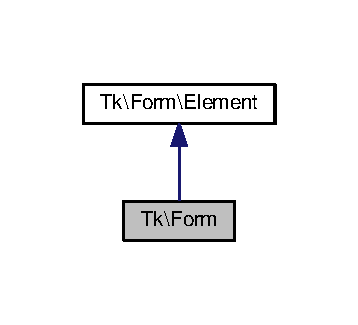
\includegraphics[width=172pt]{classTk_1_1Form__inherit__graph}
\end{center}
\end{figure}
\subsection*{Public Member Functions}
\begin{DoxyCompactItemize}
\item 
\hyperlink{classTk_1_1Form_ae9d2adc13998c0d8235e8ccd72502379}{\+\_\+\+\_\+construct} (\$form\+Id, \$params=array(), \$request=null)
\item 
\hyperlink{classTk_1_1Form_a9f326acf88301f2dfedc6207d46f3b3c}{get\+Id} ()
\item 
\hyperlink{classTk_1_1Form_a158a24883b432d44c8026c530e318476}{get\+Param} (\$name)
\item 
\hyperlink{classTk_1_1Form_ab7ef439d6244a7a1e26379dd8d40d9a1}{add\+Param} (\$name, \$value)
\item 
\hyperlink{classTk_1_1Form_a14ceaba4e12b17a98ba8fb072bfe3dfc}{get\+Params} ()
\item 
\hyperlink{classTk_1_1Form_a3f9504ad3a60ffdebed195f3d18b54ee}{set\+Params} (\$params)
\item 
\& \hyperlink{classTk_1_1Form_aa782ecaad585c31a4909d7d1f02993fc}{get\+Request} ()
\item 
\hyperlink{classTk_1_1Form_ab556964effdbc6855033c5015d7b677a}{get\+Triggered\+Event} ()
\item 
\hyperlink{classTk_1_1Form_ac8a33e8688d09999bce46c22c93a3f73}{set\+Event\+Callback} (\$name, \$callback)
\item 
\hyperlink{classTk_1_1Form_a2eb85384e0c0bdc88304961405a9236c}{is\+Submitted} ()
\item 
\hyperlink{classTk_1_1Form_ae9d0fd2f206bc8b059649819c9794a8c}{load\+From\+String} (\$array)
\item 
\hyperlink{classTk_1_1Form_a7b26b4e41292576b08e65d67ff38ec5a}{load\+From\+Object} (\$object)
\item 
\hyperlink{classTk_1_1Form_a9e9675f4e1207457b25c12bec098ccdb}{get\+Values} ()
\item 
\hyperlink{classTk_1_1Form_a7394db68dd5042a6bf1ce61a419fbf8e}{get\+String\+Values} ()
\item 
\hyperlink{classTk_1_1Form_a76c65ab7506669afee654274961b995d}{add\+Field} (\$field)
\item 
\hyperlink{classTk_1_1Form_a3aee4b0da6dd94939d727dec95f751db}{add\+Field\+Before} (\$field\+Name, \$new\+Field)
\item 
\hyperlink{classTk_1_1Form_a5c8613f3a4ce5db902f4c7c0c122c4e1}{add\+Field\+After} (\$field\+Name, \$new\+Field)
\item 
\hyperlink{classTk_1_1Form_a2a11f4b75c432508f3ad29b3e4e1e0bc}{remove\+Field} (\$field\+Name)
\item 
\hyperlink{classTk_1_1Form_a6e5befa1ff20bfc86c3427a693d752e7}{get\+Field} (\$name)
\item 
\hyperlink{classTk_1_1Form_a0b5e39683e89cb3ea419969833f5407d}{set\+Field\+List} (\$arr=array())
\item 
\hyperlink{classTk_1_1Form_a94e79b6019f09549be8ac2b5620d0105}{get\+Field\+List} ()
\item 
\hyperlink{classTk_1_1Form_ae03b790641d33cf213092c7b5bbf4174}{get\+Field\+Value} (\$name)
\item 
\hyperlink{classTk_1_1Form_a8857cc531cc7603af37676d33ef7663d}{set\+Field\+Value} (\$name, \$value)
\item 
\hyperlink{classTk_1_1Form_afa198380530a6523e14e1e97a9b0bc70}{has\+Errors} ()
\item 
\hyperlink{classTk_1_1Form_a23f6d1c45ce31a6e203a66ad686f5283}{get\+All\+Errors} ()
\item 
\hyperlink{classTk_1_1Form_a43e37546960eaf71ce3b5e8636d25234}{add\+Field\+Error} (\$name, \$msg)
\item 
\hyperlink{classTk_1_1Form_a33777899fb9ad9b5c7ddb7f01cef5904}{add\+Field\+Errors} (\$errors)
\end{DoxyCompactItemize}
\subsection*{Public Attributes}
\begin{DoxyCompactItemize}
\item 
\hypertarget{classTk_1_1Form_a384f7f2e18317e64af46ba6cfe8b2f9b}{const {\bfseries E\+N\+C\+T\+Y\+P\+E\+\_\+\+U\+R\+L\+E\+N\+C\+O\+D\+E\+D} = 'application/x-\/www-\/form-\/urlencoded'}\label{classTk_1_1Form_a384f7f2e18317e64af46ba6cfe8b2f9b}

\item 
\hypertarget{classTk_1_1Form_acfa66dcef632e23b257c5a4a2fba13d7}{const {\bfseries E\+N\+C\+T\+Y\+P\+E\+\_\+\+M\+U\+L\+T\+I\+P\+A\+R\+T} = 'multipart/form-\/data'}\label{classTk_1_1Form_acfa66dcef632e23b257c5a4a2fba13d7}

\item 
\hypertarget{classTk_1_1Form_a735b3dfc7c580719ab51784cb1acdfd5}{const {\bfseries E\+N\+C\+T\+Y\+P\+E\+\_\+\+P\+L\+A\+I\+N} = 'text/plain'}\label{classTk_1_1Form_a735b3dfc7c580719ab51784cb1acdfd5}

\item 
\hypertarget{classTk_1_1Form_a1e75e9ce94aee02b760b607701b64b96}{const {\bfseries M\+E\+T\+H\+O\+D\+\_\+\+P\+O\+S\+T} = 'post'}\label{classTk_1_1Form_a1e75e9ce94aee02b760b607701b64b96}

\item 
\hypertarget{classTk_1_1Form_a4d6c69380b555b3948fea5b35eb75df5}{const {\bfseries M\+E\+T\+H\+O\+D\+\_\+\+G\+E\+T} = 'get'}\label{classTk_1_1Form_a4d6c69380b555b3948fea5b35eb75df5}

\end{DoxyCompactItemize}
\subsection*{Protected Attributes}
\begin{DoxyCompactItemize}
\item 
\hypertarget{classTk_1_1Form_a39a7ef47b6c0f84d0c18fabea1b3c453}{{\bfseries \$id} = ''}\label{classTk_1_1Form_a39a7ef47b6c0f84d0c18fabea1b3c453}

\item 
\hypertarget{classTk_1_1Form_a5dee60edce0fd29f9561f48a29c73257}{{\bfseries \$field\+List} = array()}\label{classTk_1_1Form_a5dee60edce0fd29f9561f48a29c73257}

\item 
\hypertarget{classTk_1_1Form_a2c3ca7ebf4c63f022b6c70744df1650b}{{\bfseries \$triggered\+Event} = null}\label{classTk_1_1Form_a2c3ca7ebf4c63f022b6c70744df1650b}

\item 
\hypertarget{classTk_1_1Form_a280193bb64799739652ea8e073aa0209}{{\bfseries \$params} = null}\label{classTk_1_1Form_a280193bb64799739652ea8e073aa0209}

\item 
\hypertarget{classTk_1_1Form_a14f81c5126c5b7de30ba228b4af9a2c8}{{\bfseries \$request} = null}\label{classTk_1_1Form_a14f81c5126c5b7de30ba228b4af9a2c8}

\end{DoxyCompactItemize}


\subsection{Detailed Description}
The dynamic form processor

{\ttfamily enctype} Attribute Values\+: {\ttfamily  \begin{TabularC}{2}
\hline
\rowcolor{lightgray}{\bf Value }&{\bf Description  }\\\cline{1-2}
application/x-\/www-\/form-\/urlencoded &All characters are encoded before sent (this is default) \\\cline{1-2}
multipart/form-\/data &No characters are encoded. This value is required when you are using forms that have a file upload control \\\cline{1-2}
text/plain &Spaces are converted to \char`\"{}+\char`\"{} symbols, but no special characters are encoded \\\cline{1-2}
\end{TabularC}
}

accept-\/charset is set as the \$encoding parameter or use set\+Encoding()

\begin{DoxyAuthor}{Author}
Michael Mifsud \href{mailto:info@tropotek.com}{\tt info@tropotek.\+com} \hyperlink{}{Copyright 2015 Michael Mifsud }
\end{DoxyAuthor}


\subsection{Constructor \& Destructor Documentation}
\hypertarget{classTk_1_1Form_ae9d2adc13998c0d8235e8ccd72502379}{\index{Tk\+::\+Form@{Tk\+::\+Form}!\+\_\+\+\_\+construct@{\+\_\+\+\_\+construct}}
\index{\+\_\+\+\_\+construct@{\+\_\+\+\_\+construct}!Tk\+::\+Form@{Tk\+::\+Form}}
\subsubsection[{\+\_\+\+\_\+construct}]{\setlength{\rightskip}{0pt plus 5cm}Tk\textbackslash{}\+Form\+::\+\_\+\+\_\+construct (
\begin{DoxyParamCaption}
\item[{}]{\$form\+Id, }
\item[{}]{\$params = {\ttfamily array()}, }
\item[{}]{\$request = {\ttfamily null}}
\end{DoxyParamCaption}
)}}\label{classTk_1_1Form_ae9d2adc13998c0d8235e8ccd72502379}
Create a form processor


\begin{DoxyParams}[1]{Parameters}
string & {\em \$form\+Id} & \\
\hline
array & {\em \$params} & An array containing parameters that you may need for extending the form \\
\hline
array | \textbackslash{}\+Array\+Access & {\em \$request} & \\
\hline
\end{DoxyParams}


\subsection{Member Function Documentation}
\hypertarget{classTk_1_1Form_a76c65ab7506669afee654274961b995d}{\index{Tk\+::\+Form@{Tk\+::\+Form}!add\+Field@{add\+Field}}
\index{add\+Field@{add\+Field}!Tk\+::\+Form@{Tk\+::\+Form}}
\subsubsection[{add\+Field}]{\setlength{\rightskip}{0pt plus 5cm}Tk\textbackslash{}\+Form\+::add\+Field (
\begin{DoxyParamCaption}
\item[{}]{\$field}
\end{DoxyParamCaption}
)}}\label{classTk_1_1Form_a76c65ab7506669afee654274961b995d}
Add an field to this form


\begin{DoxyParams}[1]{Parameters}
Field\textbackslash{}\+Iface & {\em \$field} & \\
\hline
\end{DoxyParams}
\begin{DoxyReturn}{Returns}
Field 
\end{DoxyReturn}
\hypertarget{classTk_1_1Form_a5c8613f3a4ce5db902f4c7c0c122c4e1}{\index{Tk\+::\+Form@{Tk\+::\+Form}!add\+Field\+After@{add\+Field\+After}}
\index{add\+Field\+After@{add\+Field\+After}!Tk\+::\+Form@{Tk\+::\+Form}}
\subsubsection[{add\+Field\+After}]{\setlength{\rightskip}{0pt plus 5cm}Tk\textbackslash{}\+Form\+::add\+Field\+After (
\begin{DoxyParamCaption}
\item[{}]{\$field\+Name, }
\item[{}]{\$new\+Field}
\end{DoxyParamCaption}
)}}\label{classTk_1_1Form_a5c8613f3a4ce5db902f4c7c0c122c4e1}
Add an element after another element


\begin{DoxyParams}[1]{Parameters}
string & {\em \$field\+Name} & \\
\hline
Field\textbackslash{}\+Iface & {\em \$new\+Field} & \\
\hline
\end{DoxyParams}
\begin{DoxyReturn}{Returns}
Field 
\end{DoxyReturn}
\hypertarget{classTk_1_1Form_a3aee4b0da6dd94939d727dec95f751db}{\index{Tk\+::\+Form@{Tk\+::\+Form}!add\+Field\+Before@{add\+Field\+Before}}
\index{add\+Field\+Before@{add\+Field\+Before}!Tk\+::\+Form@{Tk\+::\+Form}}
\subsubsection[{add\+Field\+Before}]{\setlength{\rightskip}{0pt plus 5cm}Tk\textbackslash{}\+Form\+::add\+Field\+Before (
\begin{DoxyParamCaption}
\item[{}]{\$field\+Name, }
\item[{}]{\$new\+Field}
\end{DoxyParamCaption}
)}}\label{classTk_1_1Form_a3aee4b0da6dd94939d727dec95f751db}
Add a field element before another element


\begin{DoxyParams}[1]{Parameters}
string & {\em \$field\+Name} & \\
\hline
Field\textbackslash{}\+Iface & {\em \$new\+Field} & \\
\hline
\end{DoxyParams}
\begin{DoxyReturn}{Returns}
Field 
\end{DoxyReturn}
\hypertarget{classTk_1_1Form_a43e37546960eaf71ce3b5e8636d25234}{\index{Tk\+::\+Form@{Tk\+::\+Form}!add\+Field\+Error@{add\+Field\+Error}}
\index{add\+Field\+Error@{add\+Field\+Error}!Tk\+::\+Form@{Tk\+::\+Form}}
\subsubsection[{add\+Field\+Error}]{\setlength{\rightskip}{0pt plus 5cm}Tk\textbackslash{}\+Form\+::add\+Field\+Error (
\begin{DoxyParamCaption}
\item[{}]{\$name, }
\item[{}]{\$msg}
\end{DoxyParamCaption}
)}}\label{classTk_1_1Form_a43e37546960eaf71ce3b5e8636d25234}
Adds field error.

If the field is not found in the form then the error message is set to the form error message.

If \$msg is null the field's error list is cleared


\begin{DoxyParams}[1]{Parameters}
string & {\em \$name} & A field name. \\
\hline
string & {\em \$msg} & The error message. \\
\hline
\end{DoxyParams}
\hypertarget{classTk_1_1Form_a33777899fb9ad9b5c7ddb7f01cef5904}{\index{Tk\+::\+Form@{Tk\+::\+Form}!add\+Field\+Errors@{add\+Field\+Errors}}
\index{add\+Field\+Errors@{add\+Field\+Errors}!Tk\+::\+Form@{Tk\+::\+Form}}
\subsubsection[{add\+Field\+Errors}]{\setlength{\rightskip}{0pt plus 5cm}Tk\textbackslash{}\+Form\+::add\+Field\+Errors (
\begin{DoxyParamCaption}
\item[{}]{\$errors}
\end{DoxyParamCaption}
)}}\label{classTk_1_1Form_a33777899fb9ad9b5c7ddb7f01cef5904}
Adds form field errors from a map of (field name, list of errors) message pairs.

If the field is not found in the form then the error message is added to the form error messages.


\begin{DoxyParams}[1]{Parameters}
array & {\em \$errors} & \\
\hline
\end{DoxyParams}
\hypertarget{classTk_1_1Form_ab7ef439d6244a7a1e26379dd8d40d9a1}{\index{Tk\+::\+Form@{Tk\+::\+Form}!add\+Param@{add\+Param}}
\index{add\+Param@{add\+Param}!Tk\+::\+Form@{Tk\+::\+Form}}
\subsubsection[{add\+Param}]{\setlength{\rightskip}{0pt plus 5cm}Tk\textbackslash{}\+Form\+::add\+Param (
\begin{DoxyParamCaption}
\item[{}]{\$name, }
\item[{}]{\$value}
\end{DoxyParamCaption}
)}}\label{classTk_1_1Form_ab7ef439d6244a7a1e26379dd8d40d9a1}

\begin{DoxyParams}[1]{Parameters}
string & {\em \$name} & \\
\hline
mixed & {\em \$value} & \\
\hline
\end{DoxyParams}
\begin{DoxyReturn}{Returns}
\$this 
\end{DoxyReturn}
\hypertarget{classTk_1_1Form_a23f6d1c45ce31a6e203a66ad686f5283}{\index{Tk\+::\+Form@{Tk\+::\+Form}!get\+All\+Errors@{get\+All\+Errors}}
\index{get\+All\+Errors@{get\+All\+Errors}!Tk\+::\+Form@{Tk\+::\+Form}}
\subsubsection[{get\+All\+Errors}]{\setlength{\rightskip}{0pt plus 5cm}Tk\textbackslash{}\+Form\+::get\+All\+Errors (
\begin{DoxyParamCaption}
{}
\end{DoxyParamCaption}
)}}\label{classTk_1_1Form_a23f6d1c45ce31a6e203a66ad686f5283}
Get all the errors associated with this forms request

\begin{DoxyReturn}{Returns}
array 
\end{DoxyReturn}
\hypertarget{classTk_1_1Form_a6e5befa1ff20bfc86c3427a693d752e7}{\index{Tk\+::\+Form@{Tk\+::\+Form}!get\+Field@{get\+Field}}
\index{get\+Field@{get\+Field}!Tk\+::\+Form@{Tk\+::\+Form}}
\subsubsection[{get\+Field}]{\setlength{\rightskip}{0pt plus 5cm}Tk\textbackslash{}\+Form\+::get\+Field (
\begin{DoxyParamCaption}
\item[{}]{\$name}
\end{DoxyParamCaption}
)}}\label{classTk_1_1Form_a6e5befa1ff20bfc86c3427a693d752e7}
Return a field object or null if not found


\begin{DoxyParams}[1]{Parameters}
string & {\em \$name} & \\
\hline
\end{DoxyParams}
\begin{DoxyReturn}{Returns}
Field 
\end{DoxyReturn}
\hypertarget{classTk_1_1Form_a94e79b6019f09549be8ac2b5620d0105}{\index{Tk\+::\+Form@{Tk\+::\+Form}!get\+Field\+List@{get\+Field\+List}}
\index{get\+Field\+List@{get\+Field\+List}!Tk\+::\+Form@{Tk\+::\+Form}}
\subsubsection[{get\+Field\+List}]{\setlength{\rightskip}{0pt plus 5cm}Tk\textbackslash{}\+Form\+::get\+Field\+List (
\begin{DoxyParamCaption}
{}
\end{DoxyParamCaption}
)}}\label{classTk_1_1Form_a94e79b6019f09549be8ac2b5620d0105}
Get the field array

\begin{DoxyReturn}{Returns}
array 
\end{DoxyReturn}
\hypertarget{classTk_1_1Form_ae03b790641d33cf213092c7b5bbf4174}{\index{Tk\+::\+Form@{Tk\+::\+Form}!get\+Field\+Value@{get\+Field\+Value}}
\index{get\+Field\+Value@{get\+Field\+Value}!Tk\+::\+Form@{Tk\+::\+Form}}
\subsubsection[{get\+Field\+Value}]{\setlength{\rightskip}{0pt plus 5cm}Tk\textbackslash{}\+Form\+::get\+Field\+Value (
\begin{DoxyParamCaption}
\item[{}]{\$name}
\end{DoxyParamCaption}
)}}\label{classTk_1_1Form_ae03b790641d33cf213092c7b5bbf4174}
Returns a form field value. Returns N\+U\+L\+L if no field exists


\begin{DoxyParams}[1]{Parameters}
string & {\em \$name} & The element type name. \\
\hline
\end{DoxyParams}
\begin{DoxyReturn}{Returns}
Field 
\end{DoxyReturn}
\hypertarget{classTk_1_1Form_a9f326acf88301f2dfedc6207d46f3b3c}{\index{Tk\+::\+Form@{Tk\+::\+Form}!get\+Id@{get\+Id}}
\index{get\+Id@{get\+Id}!Tk\+::\+Form@{Tk\+::\+Form}}
\subsubsection[{get\+Id}]{\setlength{\rightskip}{0pt plus 5cm}Tk\textbackslash{}\+Form\+::get\+Id (
\begin{DoxyParamCaption}
{}
\end{DoxyParamCaption}
)}}\label{classTk_1_1Form_a9f326acf88301f2dfedc6207d46f3b3c}
Get the unique id for this element

\begin{DoxyReturn}{Returns}
string 
\end{DoxyReturn}
\hypertarget{classTk_1_1Form_a158a24883b432d44c8026c530e318476}{\index{Tk\+::\+Form@{Tk\+::\+Form}!get\+Param@{get\+Param}}
\index{get\+Param@{get\+Param}!Tk\+::\+Form@{Tk\+::\+Form}}
\subsubsection[{get\+Param}]{\setlength{\rightskip}{0pt plus 5cm}Tk\textbackslash{}\+Form\+::get\+Param (
\begin{DoxyParamCaption}
\item[{}]{\$name}
\end{DoxyParamCaption}
)}}\label{classTk_1_1Form_a158a24883b432d44c8026c530e318476}
Get a parameter from the array


\begin{DoxyParams}{Parameters}
{\em \$name} & \\
\hline
\end{DoxyParams}
\begin{DoxyReturn}{Returns}
bool 
\end{DoxyReturn}
\hypertarget{classTk_1_1Form_a14ceaba4e12b17a98ba8fb072bfe3dfc}{\index{Tk\+::\+Form@{Tk\+::\+Form}!get\+Params@{get\+Params}}
\index{get\+Params@{get\+Params}!Tk\+::\+Form@{Tk\+::\+Form}}
\subsubsection[{get\+Params}]{\setlength{\rightskip}{0pt plus 5cm}Tk\textbackslash{}\+Form\+::get\+Params (
\begin{DoxyParamCaption}
{}
\end{DoxyParamCaption}
)}}\label{classTk_1_1Form_a14ceaba4e12b17a98ba8fb072bfe3dfc}
Get the param array

\begin{DoxyReturn}{Returns}
array 
\end{DoxyReturn}
\hypertarget{classTk_1_1Form_aa782ecaad585c31a4909d7d1f02993fc}{\index{Tk\+::\+Form@{Tk\+::\+Form}!get\+Request@{get\+Request}}
\index{get\+Request@{get\+Request}!Tk\+::\+Form@{Tk\+::\+Form}}
\subsubsection[{get\+Request}]{\setlength{\rightskip}{0pt plus 5cm}\& Tk\textbackslash{}\+Form\+::get\+Request (
\begin{DoxyParamCaption}
{}
\end{DoxyParamCaption}
)}}\label{classTk_1_1Form_aa782ecaad585c31a4909d7d1f02993fc}
\begin{DoxyReturn}{Returns}
array$\vert$ 
\end{DoxyReturn}
\hypertarget{classTk_1_1Form_a7394db68dd5042a6bf1ce61a419fbf8e}{\index{Tk\+::\+Form@{Tk\+::\+Form}!get\+String\+Values@{get\+String\+Values}}
\index{get\+String\+Values@{get\+String\+Values}!Tk\+::\+Form@{Tk\+::\+Form}}
\subsubsection[{get\+String\+Values}]{\setlength{\rightskip}{0pt plus 5cm}Tk\textbackslash{}\+Form\+::get\+String\+Values (
\begin{DoxyParamCaption}
{}
\end{DoxyParamCaption}
)}}\label{classTk_1_1Form_a7394db68dd5042a6bf1ce61a419fbf8e}
Return an array of the fields raw string values

\begin{DoxyReturn}{Returns}
array 
\end{DoxyReturn}
\hypertarget{classTk_1_1Form_ab556964effdbc6855033c5015d7b677a}{\index{Tk\+::\+Form@{Tk\+::\+Form}!get\+Triggered\+Event@{get\+Triggered\+Event}}
\index{get\+Triggered\+Event@{get\+Triggered\+Event}!Tk\+::\+Form@{Tk\+::\+Form}}
\subsubsection[{get\+Triggered\+Event}]{\setlength{\rightskip}{0pt plus 5cm}Tk\textbackslash{}\+Form\+::get\+Triggered\+Event (
\begin{DoxyParamCaption}
{}
\end{DoxyParamCaption}
)}}\label{classTk_1_1Form_ab556964effdbc6855033c5015d7b677a}
Get the field event to execute

This will only return a valid value {\bfseries after} the execute() method has been called.

\begin{DoxyReturn}{Returns}
Field 
\end{DoxyReturn}
\hypertarget{classTk_1_1Form_a9e9675f4e1207457b25c12bec098ccdb}{\index{Tk\+::\+Form@{Tk\+::\+Form}!get\+Values@{get\+Values}}
\index{get\+Values@{get\+Values}!Tk\+::\+Form@{Tk\+::\+Form}}
\subsubsection[{get\+Values}]{\setlength{\rightskip}{0pt plus 5cm}Tk\textbackslash{}\+Form\+::get\+Values (
\begin{DoxyParamCaption}
{}
\end{DoxyParamCaption}
)}}\label{classTk_1_1Form_a9e9675f4e1207457b25c12bec098ccdb}
This will return an array of the field's values as complex types,

\begin{DoxyReturn}{Returns}
array 
\end{DoxyReturn}
\hypertarget{classTk_1_1Form_afa198380530a6523e14e1e97a9b0bc70}{\index{Tk\+::\+Form@{Tk\+::\+Form}!has\+Errors@{has\+Errors}}
\index{has\+Errors@{has\+Errors}!Tk\+::\+Form@{Tk\+::\+Form}}
\subsubsection[{has\+Errors}]{\setlength{\rightskip}{0pt plus 5cm}Tk\textbackslash{}\+Form\+::has\+Errors (
\begin{DoxyParamCaption}
{}
\end{DoxyParamCaption}
)}}\label{classTk_1_1Form_afa198380530a6523e14e1e97a9b0bc70}
Does this form contain errors

\begin{DoxyReturn}{Returns}
bool 
\end{DoxyReturn}
\hypertarget{classTk_1_1Form_a2eb85384e0c0bdc88304961405a9236c}{\index{Tk\+::\+Form@{Tk\+::\+Form}!is\+Submitted@{is\+Submitted}}
\index{is\+Submitted@{is\+Submitted}!Tk\+::\+Form@{Tk\+::\+Form}}
\subsubsection[{is\+Submitted}]{\setlength{\rightskip}{0pt plus 5cm}Tk\textbackslash{}\+Form\+::is\+Submitted (
\begin{DoxyParamCaption}
{}
\end{DoxyParamCaption}
)}}\label{classTk_1_1Form_a2eb85384e0c0bdc88304961405a9236c}
Check if the form has been submitted

\begin{DoxyReturn}{Returns}
bool 
\end{DoxyReturn}
\hypertarget{classTk_1_1Form_a7b26b4e41292576b08e65d67ff38ec5a}{\index{Tk\+::\+Form@{Tk\+::\+Form}!load\+From\+Object@{load\+From\+Object}}
\index{load\+From\+Object@{load\+From\+Object}!Tk\+::\+Form@{Tk\+::\+Form}}
\subsubsection[{load\+From\+Object}]{\setlength{\rightskip}{0pt plus 5cm}Tk\textbackslash{}\+Form\+::load\+From\+Object (
\begin{DoxyParamCaption}
\item[{}]{\$object}
\end{DoxyParamCaption}
)}}\label{classTk_1_1Form_a7b26b4e41292576b08e65d67ff38ec5a}
Loads the form fields from the object using the fields complex type.

This can be an array or object that contains the field's values as their complex type, I\+E\+:  for a Date field and so on...


\begin{DoxyParams}[1]{Parameters}
object & {\em \$object} & The object being mapped. \\
\hline
\end{DoxyParams}
\begin{DoxyReturn}{Returns}
\$this 
\end{DoxyReturn}
\hypertarget{classTk_1_1Form_ae9d0fd2f206bc8b059649819c9794a8c}{\index{Tk\+::\+Form@{Tk\+::\+Form}!load\+From\+String@{load\+From\+String}}
\index{load\+From\+String@{load\+From\+String}!Tk\+::\+Form@{Tk\+::\+Form}}
\subsubsection[{load\+From\+String}]{\setlength{\rightskip}{0pt plus 5cm}Tk\textbackslash{}\+Form\+::load\+From\+String (
\begin{DoxyParamCaption}
\item[{}]{\$array}
\end{DoxyParamCaption}
)}}\label{classTk_1_1Form_ae9d0fd2f206bc8b059649819c9794a8c}
Loads the form with the array. This array must be in basic type form, for example like the \$\+\_\+\+R\+E\+Q\+U\+E\+S\+T, \$\+\_\+\+G\+E\+T or \$\+\_\+\+P\+O\+S\+T array from a form. E\+G\+: \$array\mbox{[}'field1'\mbox{]} = 'value1';


\begin{DoxyParams}[1]{Parameters}
array | \textbackslash{}\+Array\+Access & {\em \$array} & \\
\hline
\end{DoxyParams}
\begin{DoxyReturn}{Returns}
\$this 
\end{DoxyReturn}
\hypertarget{classTk_1_1Form_a2a11f4b75c432508f3ad29b3e4e1e0bc}{\index{Tk\+::\+Form@{Tk\+::\+Form}!remove\+Field@{remove\+Field}}
\index{remove\+Field@{remove\+Field}!Tk\+::\+Form@{Tk\+::\+Form}}
\subsubsection[{remove\+Field}]{\setlength{\rightskip}{0pt plus 5cm}Tk\textbackslash{}\+Form\+::remove\+Field (
\begin{DoxyParamCaption}
\item[{}]{\$field\+Name}
\end{DoxyParamCaption}
)}}\label{classTk_1_1Form_a2a11f4b75c432508f3ad29b3e4e1e0bc}
Remove a field from the form


\begin{DoxyParams}[1]{Parameters}
string & {\em \$field\+Name} & \\
\hline
\end{DoxyParams}
\begin{DoxyReturn}{Returns}
boolean 
\end{DoxyReturn}
\hypertarget{classTk_1_1Form_ac8a33e8688d09999bce46c22c93a3f73}{\index{Tk\+::\+Form@{Tk\+::\+Form}!set\+Event\+Callback@{set\+Event\+Callback}}
\index{set\+Event\+Callback@{set\+Event\+Callback}!Tk\+::\+Form@{Tk\+::\+Form}}
\subsubsection[{set\+Event\+Callback}]{\setlength{\rightskip}{0pt plus 5cm}Tk\textbackslash{}\+Form\+::set\+Event\+Callback (
\begin{DoxyParamCaption}
\item[{}]{\$name, }
\item[{}]{\$callback}
\end{DoxyParamCaption}
)}}\label{classTk_1_1Form_ac8a33e8688d09999bce46c22c93a3f73}
Set the callback to an event element, The element must be of the type 


\begin{DoxyParams}[1]{Parameters}
string & {\em \$name} & \\
\hline
callable & {\em \$callback} & \\
\hline
\end{DoxyParams}
\begin{DoxyReturn}{Returns}
Field 
\end{DoxyReturn}

\begin{DoxyExceptions}{Exceptions}
{\em \hyperlink{classTk_1_1Form_1_1Exception}{Exception}} & \\
\hline
\end{DoxyExceptions}
\hypertarget{classTk_1_1Form_a0b5e39683e89cb3ea419969833f5407d}{\index{Tk\+::\+Form@{Tk\+::\+Form}!set\+Field\+List@{set\+Field\+List}}
\index{set\+Field\+List@{set\+Field\+List}!Tk\+::\+Form@{Tk\+::\+Form}}
\subsubsection[{set\+Field\+List}]{\setlength{\rightskip}{0pt plus 5cm}Tk\textbackslash{}\+Form\+::set\+Field\+List (
\begin{DoxyParamCaption}
\item[{}]{\$arr = {\ttfamily array()}}
\end{DoxyParamCaption}
)}}\label{classTk_1_1Form_a0b5e39683e89cb3ea419969833f5407d}
Set the field array


\begin{DoxyParams}[1]{Parameters}
array & {\em \$arr} & \\
\hline
\end{DoxyParams}
\begin{DoxyReturn}{Returns}
\$this 
\end{DoxyReturn}
\hypertarget{classTk_1_1Form_a8857cc531cc7603af37676d33ef7663d}{\index{Tk\+::\+Form@{Tk\+::\+Form}!set\+Field\+Value@{set\+Field\+Value}}
\index{set\+Field\+Value@{set\+Field\+Value}!Tk\+::\+Form@{Tk\+::\+Form}}
\subsubsection[{set\+Field\+Value}]{\setlength{\rightskip}{0pt plus 5cm}Tk\textbackslash{}\+Form\+::set\+Field\+Value (
\begin{DoxyParamCaption}
\item[{}]{\$name, }
\item[{}]{\$value}
\end{DoxyParamCaption}
)}}\label{classTk_1_1Form_a8857cc531cc7603af37676d33ef7663d}
Sets the value of an element type.


\begin{DoxyParams}[1]{Parameters}
string & {\em \$name} & The field name. \\
\hline
mixed & {\em \$value} & The field value. \\
\hline
\end{DoxyParams}
\begin{DoxyReturn}{Returns}
Field 
\end{DoxyReturn}

\begin{DoxyExceptions}{Exceptions}
{\em \hyperlink{classTk_1_1Form_1_1Exception}{Exception}} & \\
\hline
\end{DoxyExceptions}
\hypertarget{classTk_1_1Form_a3f9504ad3a60ffdebed195f3d18b54ee}{\index{Tk\+::\+Form@{Tk\+::\+Form}!set\+Params@{set\+Params}}
\index{set\+Params@{set\+Params}!Tk\+::\+Form@{Tk\+::\+Form}}
\subsubsection[{set\+Params}]{\setlength{\rightskip}{0pt plus 5cm}Tk\textbackslash{}\+Form\+::set\+Params (
\begin{DoxyParamCaption}
\item[{}]{\$params}
\end{DoxyParamCaption}
)}}\label{classTk_1_1Form_a3f9504ad3a60ffdebed195f3d18b54ee}

\begin{DoxyParams}[1]{Parameters}
array & {\em \$params} & \\
\hline
\end{DoxyParams}


The documentation for this class was generated from the following file\+:\begin{DoxyCompactItemize}
\item 
vendor/ttek/tk-\/form/\+Tk/Form.\+php\end{DoxyCompactItemize}

\hypertarget{classApp_1_1Form_1_1FormHelper}{\section{App\textbackslash{}Form\textbackslash{}Form\+Helper Class Reference}
\label{classApp_1_1Form_1_1FormHelper}\index{App\textbackslash{}\+Form\textbackslash{}\+Form\+Helper@{App\textbackslash{}\+Form\textbackslash{}\+Form\+Helper}}
}
\subsection*{Static Public Member Functions}
\begin{DoxyCompactItemize}
\item 
static \hyperlink{classApp_1_1Form_1_1FormHelper_a2343e291e67c75145cb4d5ad6deca7f9}{create\+Form} (\textbackslash{}\hyperlink{classDom_1_1Form}{Dom\textbackslash{}\+Form} \$dom\+Form)
\end{DoxyCompactItemize}


\subsection{Detailed Description}
Use this helper for purely inline rendered forms.

This helper will create a from from the D\+O\+M template

All types will be set as a , however the buttons will be set as  objects

\begin{DoxyAuthor}{Author}
Michael Mifsud \href{mailto:info@tropotek.com}{\tt info@tropotek.\+com} \hyperlink{}{Copyright 2015 Michael Mifsud }
\end{DoxyAuthor}


\subsection{Member Function Documentation}
\hypertarget{classApp_1_1Form_1_1FormHelper_a2343e291e67c75145cb4d5ad6deca7f9}{\index{App\+::\+Form\+::\+Form\+Helper@{App\+::\+Form\+::\+Form\+Helper}!create\+Form@{create\+Form}}
\index{create\+Form@{create\+Form}!App\+::\+Form\+::\+Form\+Helper@{App\+::\+Form\+::\+Form\+Helper}}
\subsubsection[{create\+Form}]{\setlength{\rightskip}{0pt plus 5cm}static App\textbackslash{}\+Form\textbackslash{}\+Form\+Helper\+::create\+Form (
\begin{DoxyParamCaption}
\item[{\textbackslash{}{\bf Dom\textbackslash{}\+Form}}]{\$dom\+Form}
\end{DoxyParamCaption}
)\hspace{0.3cm}{\ttfamily [static]}}}\label{classApp_1_1Form_1_1FormHelper_a2343e291e67c75145cb4d5ad6deca7f9}

\begin{DoxyParams}[1]{Parameters}
\textbackslash{}\+Dom\textbackslash{}\+Form & {\em \$dom\+Form} & \\
\hline
\end{DoxyParams}
\begin{DoxyReturn}{Returns}
Form 
\end{DoxyReturn}

\begin{DoxyExceptions}{Exceptions}
{\em } & Tk \\
\hline
\end{DoxyExceptions}


The documentation for this class was generated from the following file\+:\begin{DoxyCompactItemize}
\item 
src/\+App/\+Form/Form\+Helper.\+php\end{DoxyCompactItemize}

\hypertarget{classTk_1_1Form_1_1Renderer_1_1Dom_1_1FormStatic}{\section{Tk\textbackslash{}Form\textbackslash{}Renderer\textbackslash{}Dom\textbackslash{}Form\+Static Class Reference}
\label{classTk_1_1Form_1_1Renderer_1_1Dom_1_1FormStatic}\index{Tk\textbackslash{}\+Form\textbackslash{}\+Renderer\textbackslash{}\+Dom\textbackslash{}\+Form\+Static@{Tk\textbackslash{}\+Form\textbackslash{}\+Renderer\textbackslash{}\+Dom\textbackslash{}\+Form\+Static}}
}


Inheritance diagram for Tk\textbackslash{}Form\textbackslash{}Renderer\textbackslash{}Dom\textbackslash{}Form\+Static\+:\nopagebreak
\begin{figure}[H]
\begin{center}
\leavevmode
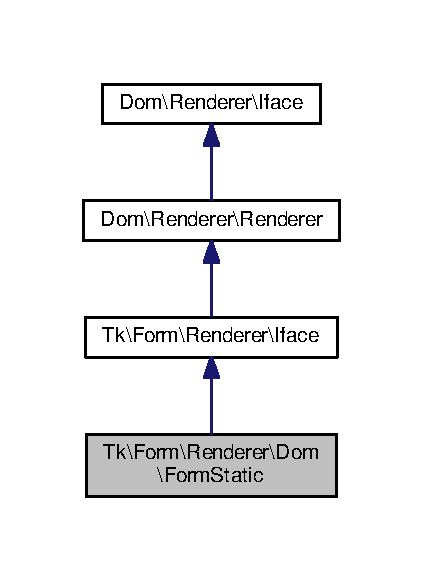
\includegraphics[width=203pt]{classTk_1_1Form_1_1Renderer_1_1Dom_1_1FormStatic__inherit__graph}
\end{center}
\end{figure}
\subsection*{Public Member Functions}
\begin{DoxyCompactItemize}
\item 
\hyperlink{classTk_1_1Form_1_1Renderer_1_1Dom_1_1FormStatic_ae4722390b401113d1692be54610c4f9f}{\+\_\+\+\_\+construct} (\$form, \$template)
\item 
\hyperlink{classTk_1_1Form_1_1Renderer_1_1Dom_1_1FormStatic_a26fa1ebf33c3504b3f599adf1070e043}{show} ()
\item 
\hyperlink{classTk_1_1Form_1_1Renderer_1_1Dom_1_1FormStatic_a3f0a6ec516a6b750bba6036c2486e3c4}{get\+First\+Child\+Element} (\$parent)
\end{DoxyCompactItemize}
\subsection*{Static Public Member Functions}
\begin{DoxyCompactItemize}
\item 
static \hyperlink{classTk_1_1Form_1_1Renderer_1_1Dom_1_1FormStatic_a7b1a3af58120ff31c17b1850aac02b88}{create} (\$form, \$template)
\end{DoxyCompactItemize}
\subsection*{Public Attributes}
\begin{DoxyCompactItemize}
\item 
\hypertarget{classTk_1_1Form_1_1Renderer_1_1Dom_1_1FormStatic_abbe112f1edcf7dad36cf1f66c001db91}{const {\bfseries M\+S\+G\+\_\+\+C\+L\+A\+S\+S\+\_\+\+E\+R\+R\+O\+R} = 'error'}\label{classTk_1_1Form_1_1Renderer_1_1Dom_1_1FormStatic_abbe112f1edcf7dad36cf1f66c001db91}

\item 
\hypertarget{classTk_1_1Form_1_1Renderer_1_1Dom_1_1FormStatic_adfb445497c1e2a0f13b567662abd6dd5}{const {\bfseries M\+S\+G\+\_\+\+C\+L\+A\+S\+S\+\_\+\+W\+A\+R\+N\+I\+N\+G} = 'warning'}\label{classTk_1_1Form_1_1Renderer_1_1Dom_1_1FormStatic_adfb445497c1e2a0f13b567662abd6dd5}

\item 
\hypertarget{classTk_1_1Form_1_1Renderer_1_1Dom_1_1FormStatic_a5a1563333aa5a577d12ead236bb52048}{const {\bfseries M\+S\+G\+\_\+\+C\+L\+A\+S\+S\+\_\+\+N\+O\+T\+I\+C\+E} = 'notice'}\label{classTk_1_1Form_1_1Renderer_1_1Dom_1_1FormStatic_a5a1563333aa5a577d12ead236bb52048}

\end{DoxyCompactItemize}
\subsection*{Protected Member Functions}
\begin{DoxyCompactItemize}
\item 
\hyperlink{classTk_1_1Form_1_1Renderer_1_1Dom_1_1FormStatic_ac051723d3350216c16cbee37cbe63b1f}{show\+Field} (\hyperlink{classTk_1_1Form_1_1Renderer_1_1Dom_1_1Field_1_1Iface}{Field\textbackslash{}\+Iface} \$field)
\item 
\hyperlink{classTk_1_1Form_1_1Renderer_1_1Dom_1_1FormStatic_a56ef6c567bcced44ee71ffdd7a6c22ec}{show\+Form\+Error} ()
\item 
\hyperlink{classTk_1_1Form_1_1Renderer_1_1Dom_1_1FormStatic_acfb647c4e2b1a98ed704dbf3e741010b}{show\+Error} (\$field)
\end{DoxyCompactItemize}
\subsection*{Protected Attributes}
\begin{DoxyCompactItemize}
\item 
\hypertarget{classTk_1_1Form_1_1Renderer_1_1Dom_1_1FormStatic_ad5c6b9ca1ce0cdd26034ca87002f4699}{{\bfseries \$dom\+Form} = null}\label{classTk_1_1Form_1_1Renderer_1_1Dom_1_1FormStatic_ad5c6b9ca1ce0cdd26034ca87002f4699}

\end{DoxyCompactItemize}


\subsection{Detailed Description}
The static form renderer. It requires on the Dom\+\_\+\+Form class

This renderer requires that the form markup is already in place.

\begin{DoxyAuthor}{Author}
Michael Mifsud \href{mailto:info@tropotek.com}{\tt info@tropotek.\+com} \hyperlink{}{Copyright 2015 Michael Mifsud }
\end{DoxyAuthor}


\subsection{Constructor \& Destructor Documentation}
\hypertarget{classTk_1_1Form_1_1Renderer_1_1Dom_1_1FormStatic_ae4722390b401113d1692be54610c4f9f}{\index{Tk\+::\+Form\+::\+Renderer\+::\+Dom\+::\+Form\+Static@{Tk\+::\+Form\+::\+Renderer\+::\+Dom\+::\+Form\+Static}!\+\_\+\+\_\+construct@{\+\_\+\+\_\+construct}}
\index{\+\_\+\+\_\+construct@{\+\_\+\+\_\+construct}!Tk\+::\+Form\+::\+Renderer\+::\+Dom\+::\+Form\+Static@{Tk\+::\+Form\+::\+Renderer\+::\+Dom\+::\+Form\+Static}}
\subsubsection[{\+\_\+\+\_\+construct}]{\setlength{\rightskip}{0pt plus 5cm}Tk\textbackslash{}\+Form\textbackslash{}\+Renderer\textbackslash{}\+Dom\textbackslash{}\+Form\+Static\+::\+\_\+\+\_\+construct (
\begin{DoxyParamCaption}
\item[{}]{\$form, }
\item[{}]{\$template}
\end{DoxyParamCaption}
)}}\label{classTk_1_1Form_1_1Renderer_1_1Dom_1_1FormStatic_ae4722390b401113d1692be54610c4f9f}
Create the object instance


\begin{DoxyParams}[1]{Parameters}
\hyperlink{classTk_1_1Form_1_1Renderer_1_1Dom_1_1Form}{Form} & {\em \$form} & \\
\hline
\textbackslash{}\+Dom\textbackslash{}\+Template & {\em \$template} & \\
\hline
\end{DoxyParams}


\subsection{Member Function Documentation}
\hypertarget{classTk_1_1Form_1_1Renderer_1_1Dom_1_1FormStatic_a7b1a3af58120ff31c17b1850aac02b88}{\index{Tk\+::\+Form\+::\+Renderer\+::\+Dom\+::\+Form\+Static@{Tk\+::\+Form\+::\+Renderer\+::\+Dom\+::\+Form\+Static}!create@{create}}
\index{create@{create}!Tk\+::\+Form\+::\+Renderer\+::\+Dom\+::\+Form\+Static@{Tk\+::\+Form\+::\+Renderer\+::\+Dom\+::\+Form\+Static}}
\subsubsection[{create}]{\setlength{\rightskip}{0pt plus 5cm}static Tk\textbackslash{}\+Form\textbackslash{}\+Renderer\textbackslash{}\+Dom\textbackslash{}\+Form\+Static\+::create (
\begin{DoxyParamCaption}
\item[{}]{\$form, }
\item[{}]{\$template}
\end{DoxyParamCaption}
)\hspace{0.3cm}{\ttfamily [static]}}}\label{classTk_1_1Form_1_1Renderer_1_1Dom_1_1FormStatic_a7b1a3af58120ff31c17b1850aac02b88}
Create a new Renderer.


\begin{DoxyParams}[1]{Parameters}
\hyperlink{classTk_1_1Form_1_1Renderer_1_1Dom_1_1Form}{Form} & {\em \$form} & \\
\hline
\textbackslash{}\+Dom\textbackslash{}\+Template & {\em \$template} & The template where the form resides \\
\hline
\end{DoxyParams}
\begin{DoxyReturn}{Returns}
\hyperlink{classTk_1_1Form_1_1Renderer_1_1Dom_1_1Form}{Form} 
\end{DoxyReturn}
\hypertarget{classTk_1_1Form_1_1Renderer_1_1Dom_1_1FormStatic_a3f0a6ec516a6b750bba6036c2486e3c4}{\index{Tk\+::\+Form\+::\+Renderer\+::\+Dom\+::\+Form\+Static@{Tk\+::\+Form\+::\+Renderer\+::\+Dom\+::\+Form\+Static}!get\+First\+Child\+Element@{get\+First\+Child\+Element}}
\index{get\+First\+Child\+Element@{get\+First\+Child\+Element}!Tk\+::\+Form\+::\+Renderer\+::\+Dom\+::\+Form\+Static@{Tk\+::\+Form\+::\+Renderer\+::\+Dom\+::\+Form\+Static}}
\subsubsection[{get\+First\+Child\+Element}]{\setlength{\rightskip}{0pt plus 5cm}Tk\textbackslash{}\+Form\textbackslash{}\+Renderer\textbackslash{}\+Dom\textbackslash{}\+Form\+Static\+::get\+First\+Child\+Element (
\begin{DoxyParamCaption}
\item[{}]{\$parent}
\end{DoxyParamCaption}
)}}\label{classTk_1_1Form_1_1Renderer_1_1Dom_1_1FormStatic_a3f0a6ec516a6b750bba6036c2486e3c4}
get\+First\+Child\+Element


\begin{DoxyParams}[1]{Parameters}
\textbackslash{}\+D\+O\+M\+Element & {\em \$parent} & \\
\hline
\end{DoxyParams}
\begin{DoxyReturn}{Returns}

\end{DoxyReturn}
\hypertarget{classTk_1_1Form_1_1Renderer_1_1Dom_1_1FormStatic_a26fa1ebf33c3504b3f599adf1070e043}{\index{Tk\+::\+Form\+::\+Renderer\+::\+Dom\+::\+Form\+Static@{Tk\+::\+Form\+::\+Renderer\+::\+Dom\+::\+Form\+Static}!show@{show}}
\index{show@{show}!Tk\+::\+Form\+::\+Renderer\+::\+Dom\+::\+Form\+Static@{Tk\+::\+Form\+::\+Renderer\+::\+Dom\+::\+Form\+Static}}
\subsubsection[{show}]{\setlength{\rightskip}{0pt plus 5cm}Tk\textbackslash{}\+Form\textbackslash{}\+Renderer\textbackslash{}\+Dom\textbackslash{}\+Form\+Static\+::show (
\begin{DoxyParamCaption}
{}
\end{DoxyParamCaption}
)}}\label{classTk_1_1Form_1_1Renderer_1_1Dom_1_1FormStatic_a26fa1ebf33c3504b3f599adf1070e043}
Render

\begin{DoxyReturn}{Returns}
mixed 
\end{DoxyReturn}


Implements \hyperlink{interfaceDom_1_1Renderer_1_1Iface_a79a0ba41fb6714d69156891d6326bd33}{Dom\textbackslash{}\+Renderer\textbackslash{}\+Iface}.

\hypertarget{classTk_1_1Form_1_1Renderer_1_1Dom_1_1FormStatic_acfb647c4e2b1a98ed704dbf3e741010b}{\index{Tk\+::\+Form\+::\+Renderer\+::\+Dom\+::\+Form\+Static@{Tk\+::\+Form\+::\+Renderer\+::\+Dom\+::\+Form\+Static}!show\+Error@{show\+Error}}
\index{show\+Error@{show\+Error}!Tk\+::\+Form\+::\+Renderer\+::\+Dom\+::\+Form\+Static@{Tk\+::\+Form\+::\+Renderer\+::\+Dom\+::\+Form\+Static}}
\subsubsection[{show\+Error}]{\setlength{\rightskip}{0pt plus 5cm}Tk\textbackslash{}\+Form\textbackslash{}\+Renderer\textbackslash{}\+Dom\textbackslash{}\+Form\+Static\+::show\+Error (
\begin{DoxyParamCaption}
\item[{}]{\$field}
\end{DoxyParamCaption}
)\hspace{0.3cm}{\ttfamily [protected]}}}\label{classTk_1_1Form_1_1Renderer_1_1Dom_1_1FormStatic_acfb647c4e2b1a98ed704dbf3e741010b}

\begin{DoxyParams}[1]{Parameters}
Field & {\em \$field} & \\
\hline
\end{DoxyParams}

\begin{DoxyExceptions}{Exceptions}
{\em \hyperlink{classTk_1_1Form_1_1Exception}{Exception}} & \\
\hline
\end{DoxyExceptions}
\hypertarget{classTk_1_1Form_1_1Renderer_1_1Dom_1_1FormStatic_ac051723d3350216c16cbee37cbe63b1f}{\index{Tk\+::\+Form\+::\+Renderer\+::\+Dom\+::\+Form\+Static@{Tk\+::\+Form\+::\+Renderer\+::\+Dom\+::\+Form\+Static}!show\+Field@{show\+Field}}
\index{show\+Field@{show\+Field}!Tk\+::\+Form\+::\+Renderer\+::\+Dom\+::\+Form\+Static@{Tk\+::\+Form\+::\+Renderer\+::\+Dom\+::\+Form\+Static}}
\subsubsection[{show\+Field}]{\setlength{\rightskip}{0pt plus 5cm}Tk\textbackslash{}\+Form\textbackslash{}\+Renderer\textbackslash{}\+Dom\textbackslash{}\+Form\+Static\+::show\+Field (
\begin{DoxyParamCaption}
\item[{{\bf Field\textbackslash{}\+Iface}}]{\$field}
\end{DoxyParamCaption}
)\hspace{0.3cm}{\ttfamily [protected]}}}\label{classTk_1_1Form_1_1Renderer_1_1Dom_1_1FormStatic_ac051723d3350216c16cbee37cbe63b1f}
Render the form field values


\begin{DoxyParams}[1]{Parameters}
Field\textbackslash{}\+Iface & {\em \$field} & \\
\hline
\end{DoxyParams}
\begin{DoxyReturn}{Returns}
mixed 
\end{DoxyReturn}

\begin{DoxyExceptions}{Exceptions}
{\em } & Tk \\
\hline
\end{DoxyExceptions}
\hypertarget{classTk_1_1Form_1_1Renderer_1_1Dom_1_1FormStatic_a56ef6c567bcced44ee71ffdd7a6c22ec}{\index{Tk\+::\+Form\+::\+Renderer\+::\+Dom\+::\+Form\+Static@{Tk\+::\+Form\+::\+Renderer\+::\+Dom\+::\+Form\+Static}!show\+Form\+Error@{show\+Form\+Error}}
\index{show\+Form\+Error@{show\+Form\+Error}!Tk\+::\+Form\+::\+Renderer\+::\+Dom\+::\+Form\+Static@{Tk\+::\+Form\+::\+Renderer\+::\+Dom\+::\+Form\+Static}}
\subsubsection[{show\+Form\+Error}]{\setlength{\rightskip}{0pt plus 5cm}Tk\textbackslash{}\+Form\textbackslash{}\+Renderer\textbackslash{}\+Dom\textbackslash{}\+Form\+Static\+::show\+Form\+Error (
\begin{DoxyParamCaption}
{}
\end{DoxyParamCaption}
)\hspace{0.3cm}{\ttfamily [protected]}}}\label{classTk_1_1Form_1_1Renderer_1_1Dom_1_1FormStatic_a56ef6c567bcced44ee71ffdd7a6c22ec}
Show the overall form error if set 

The documentation for this class was generated from the following file\+:\begin{DoxyCompactItemize}
\item 
vendor/ttek/tk-\/form/\+Tk/\+Form/\+Renderer/\+Dom/Form\+Static.\+php\end{DoxyCompactItemize}

\hypertarget{classTk_1_1Form_1_1Renderer_1_1Dom_1_1Field_1_1Hidden}{\section{Tk\textbackslash{}Form\textbackslash{}Renderer\textbackslash{}Dom\textbackslash{}Field\textbackslash{}Hidden Class Reference}
\label{classTk_1_1Form_1_1Renderer_1_1Dom_1_1Field_1_1Hidden}\index{Tk\textbackslash{}\+Form\textbackslash{}\+Renderer\textbackslash{}\+Dom\textbackslash{}\+Field\textbackslash{}\+Hidden@{Tk\textbackslash{}\+Form\textbackslash{}\+Renderer\textbackslash{}\+Dom\textbackslash{}\+Field\textbackslash{}\+Hidden}}
}


Inheritance diagram for Tk\textbackslash{}Form\textbackslash{}Renderer\textbackslash{}Dom\textbackslash{}Field\textbackslash{}Hidden\+:\nopagebreak
\begin{figure}[H]
\begin{center}
\leavevmode
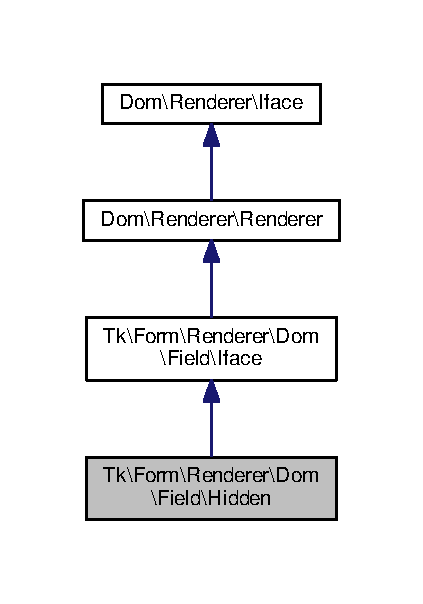
\includegraphics[width=203pt]{classTk_1_1Form_1_1Renderer_1_1Dom_1_1Field_1_1Hidden__inherit__graph}
\end{center}
\end{figure}
\subsection*{Public Member Functions}
\begin{DoxyCompactItemize}
\item 
\hyperlink{classTk_1_1Form_1_1Renderer_1_1Dom_1_1Field_1_1Hidden_a482c59511558e1e4bdf83d943fc2800d}{show} ()
\item 
\hyperlink{classTk_1_1Form_1_1Renderer_1_1Dom_1_1Field_1_1Hidden_aabe13c78d33dd8ac012e61f28936e597}{\+\_\+\+\_\+make\+Template} ()
\end{DoxyCompactItemize}
\subsection*{Additional Inherited Members}


\subsection{Detailed Description}
Class \hyperlink{classTk_1_1Form_1_1Renderer_1_1Dom_1_1Field_1_1Text}{Text}

\begin{DoxyAuthor}{Author}
Michael Mifsud \href{mailto:info@tropotek.com}{\tt info@tropotek.\+com} \hyperlink{}{Copyright 2015 Michael Mifsud }
\end{DoxyAuthor}


\subsection{Member Function Documentation}
\hypertarget{classTk_1_1Form_1_1Renderer_1_1Dom_1_1Field_1_1Hidden_aabe13c78d33dd8ac012e61f28936e597}{\index{Tk\+::\+Form\+::\+Renderer\+::\+Dom\+::\+Field\+::\+Hidden@{Tk\+::\+Form\+::\+Renderer\+::\+Dom\+::\+Field\+::\+Hidden}!\+\_\+\+\_\+make\+Template@{\+\_\+\+\_\+make\+Template}}
\index{\+\_\+\+\_\+make\+Template@{\+\_\+\+\_\+make\+Template}!Tk\+::\+Form\+::\+Renderer\+::\+Dom\+::\+Field\+::\+Hidden@{Tk\+::\+Form\+::\+Renderer\+::\+Dom\+::\+Field\+::\+Hidden}}
\subsubsection[{\+\_\+\+\_\+make\+Template}]{\setlength{\rightskip}{0pt plus 5cm}Tk\textbackslash{}\+Form\textbackslash{}\+Renderer\textbackslash{}\+Dom\textbackslash{}\+Field\textbackslash{}\+Hidden\+::\+\_\+\+\_\+make\+Template (
\begin{DoxyParamCaption}
{}
\end{DoxyParamCaption}
)}}\label{classTk_1_1Form_1_1Renderer_1_1Dom_1_1Field_1_1Hidden_aabe13c78d33dd8ac012e61f28936e597}
The default element template

\begin{DoxyReturn}{Returns}

\end{DoxyReturn}
\hypertarget{classTk_1_1Form_1_1Renderer_1_1Dom_1_1Field_1_1Hidden_a482c59511558e1e4bdf83d943fc2800d}{\index{Tk\+::\+Form\+::\+Renderer\+::\+Dom\+::\+Field\+::\+Hidden@{Tk\+::\+Form\+::\+Renderer\+::\+Dom\+::\+Field\+::\+Hidden}!show@{show}}
\index{show@{show}!Tk\+::\+Form\+::\+Renderer\+::\+Dom\+::\+Field\+::\+Hidden@{Tk\+::\+Form\+::\+Renderer\+::\+Dom\+::\+Field\+::\+Hidden}}
\subsubsection[{show}]{\setlength{\rightskip}{0pt plus 5cm}Tk\textbackslash{}\+Form\textbackslash{}\+Renderer\textbackslash{}\+Dom\textbackslash{}\+Field\textbackslash{}\+Hidden\+::show (
\begin{DoxyParamCaption}
{}
\end{DoxyParamCaption}
)}}\label{classTk_1_1Form_1_1Renderer_1_1Dom_1_1Field_1_1Hidden_a482c59511558e1e4bdf83d943fc2800d}
Render the field 

Implements \hyperlink{interfaceDom_1_1Renderer_1_1Iface_a79a0ba41fb6714d69156891d6326bd33}{Dom\textbackslash{}\+Renderer\textbackslash{}\+Iface}.



The documentation for this class was generated from the following file\+:\begin{DoxyCompactItemize}
\item 
vendor/ttek/tk-\/form/\+Tk/\+Form/\+Renderer/\+Dom/\+Field/Hidden.\+php\end{DoxyCompactItemize}

\hypertarget{classTk_1_1Form_1_1Renderer_1_1Dom_1_1Field_1_1Html}{\section{Tk\textbackslash{}Form\textbackslash{}Renderer\textbackslash{}Dom\textbackslash{}Field\textbackslash{}Html Class Reference}
\label{classTk_1_1Form_1_1Renderer_1_1Dom_1_1Field_1_1Html}\index{Tk\textbackslash{}\+Form\textbackslash{}\+Renderer\textbackslash{}\+Dom\textbackslash{}\+Field\textbackslash{}\+Html@{Tk\textbackslash{}\+Form\textbackslash{}\+Renderer\textbackslash{}\+Dom\textbackslash{}\+Field\textbackslash{}\+Html}}
}


Inheritance diagram for Tk\textbackslash{}Form\textbackslash{}Renderer\textbackslash{}Dom\textbackslash{}Field\textbackslash{}Html\+:\nopagebreak
\begin{figure}[H]
\begin{center}
\leavevmode
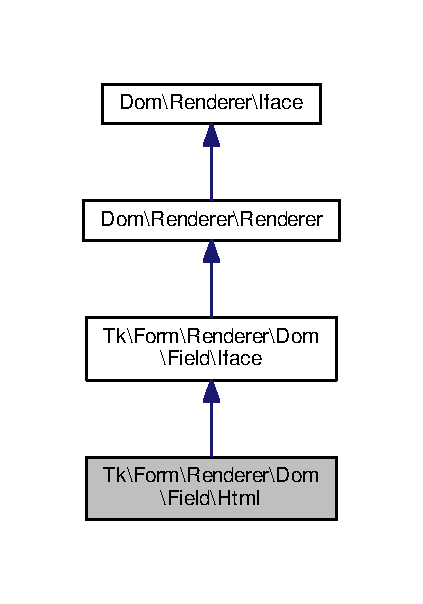
\includegraphics[width=203pt]{classTk_1_1Form_1_1Renderer_1_1Dom_1_1Field_1_1Html__inherit__graph}
\end{center}
\end{figure}
\subsection*{Public Member Functions}
\begin{DoxyCompactItemize}
\item 
\hyperlink{classTk_1_1Form_1_1Renderer_1_1Dom_1_1Field_1_1Html_a428ec264e10aad234e500ee237ea9581}{\+\_\+\+\_\+construct} (\hyperlink{classTk_1_1Form_1_1Renderer_1_1Dom_1_1Field_1_1Iface}{Field\textbackslash{}\+Iface} \$field, \$html)
\item 
\hyperlink{classTk_1_1Form_1_1Renderer_1_1Dom_1_1Field_1_1Html_abd1e07e5a157a478b8f9a3656115c5c0}{show\+Element} ()
\item 
\hyperlink{classTk_1_1Form_1_1Renderer_1_1Dom_1_1Field_1_1Html_a450ce2d85ec3feaeaa721cb27c31952c}{\+\_\+\+\_\+make\+Template} ()
\end{DoxyCompactItemize}
\subsection*{Protected Attributes}
\begin{DoxyCompactItemize}
\item 
\hypertarget{classTk_1_1Form_1_1Renderer_1_1Dom_1_1Field_1_1Html_a884c30bda19ab960d5845f77dfc83a92}{{\bfseries \$html} = ''}\label{classTk_1_1Form_1_1Renderer_1_1Dom_1_1Field_1_1Html_a884c30bda19ab960d5845f77dfc83a92}

\end{DoxyCompactItemize}


\subsection{Detailed Description}
Class \hyperlink{classTk_1_1Form_1_1Renderer_1_1Dom_1_1Field_1_1Text}{Text}

\begin{DoxyAuthor}{Author}
Michael Mifsud \href{mailto:info@tropotek.com}{\tt info@tropotek.\+com} \hyperlink{}{Copyright 2015 Michael Mifsud }
\end{DoxyAuthor}


\subsection{Constructor \& Destructor Documentation}
\hypertarget{classTk_1_1Form_1_1Renderer_1_1Dom_1_1Field_1_1Html_a428ec264e10aad234e500ee237ea9581}{\index{Tk\+::\+Form\+::\+Renderer\+::\+Dom\+::\+Field\+::\+Html@{Tk\+::\+Form\+::\+Renderer\+::\+Dom\+::\+Field\+::\+Html}!\+\_\+\+\_\+construct@{\+\_\+\+\_\+construct}}
\index{\+\_\+\+\_\+construct@{\+\_\+\+\_\+construct}!Tk\+::\+Form\+::\+Renderer\+::\+Dom\+::\+Field\+::\+Html@{Tk\+::\+Form\+::\+Renderer\+::\+Dom\+::\+Field\+::\+Html}}
\subsubsection[{\+\_\+\+\_\+construct}]{\setlength{\rightskip}{0pt plus 5cm}Tk\textbackslash{}\+Form\textbackslash{}\+Renderer\textbackslash{}\+Dom\textbackslash{}\+Field\textbackslash{}\+Html\+::\+\_\+\+\_\+construct (
\begin{DoxyParamCaption}
\item[{{\bf Field\textbackslash{}\+Iface}}]{\$field, }
\item[{}]{\$html}
\end{DoxyParamCaption}
)}}\label{classTk_1_1Form_1_1Renderer_1_1Dom_1_1Field_1_1Html_a428ec264e10aad234e500ee237ea9581}
\+\_\+\+\_\+construct


\begin{DoxyParams}[1]{Parameters}
Field\textbackslash{}\+Iface & {\em \$field} & \\
\hline
\end{DoxyParams}


\subsection{Member Function Documentation}
\hypertarget{classTk_1_1Form_1_1Renderer_1_1Dom_1_1Field_1_1Html_a450ce2d85ec3feaeaa721cb27c31952c}{\index{Tk\+::\+Form\+::\+Renderer\+::\+Dom\+::\+Field\+::\+Html@{Tk\+::\+Form\+::\+Renderer\+::\+Dom\+::\+Field\+::\+Html}!\+\_\+\+\_\+make\+Template@{\+\_\+\+\_\+make\+Template}}
\index{\+\_\+\+\_\+make\+Template@{\+\_\+\+\_\+make\+Template}!Tk\+::\+Form\+::\+Renderer\+::\+Dom\+::\+Field\+::\+Html@{Tk\+::\+Form\+::\+Renderer\+::\+Dom\+::\+Field\+::\+Html}}
\subsubsection[{\+\_\+\+\_\+make\+Template}]{\setlength{\rightskip}{0pt plus 5cm}Tk\textbackslash{}\+Form\textbackslash{}\+Renderer\textbackslash{}\+Dom\textbackslash{}\+Field\textbackslash{}\+Html\+::\+\_\+\+\_\+make\+Template (
\begin{DoxyParamCaption}
{}
\end{DoxyParamCaption}
)}}\label{classTk_1_1Form_1_1Renderer_1_1Dom_1_1Field_1_1Html_a450ce2d85ec3feaeaa721cb27c31952c}
The default element template

\begin{DoxyReturn}{Returns}

\end{DoxyReturn}
\hypertarget{classTk_1_1Form_1_1Renderer_1_1Dom_1_1Field_1_1Html_abd1e07e5a157a478b8f9a3656115c5c0}{\index{Tk\+::\+Form\+::\+Renderer\+::\+Dom\+::\+Field\+::\+Html@{Tk\+::\+Form\+::\+Renderer\+::\+Dom\+::\+Field\+::\+Html}!show\+Element@{show\+Element}}
\index{show\+Element@{show\+Element}!Tk\+::\+Form\+::\+Renderer\+::\+Dom\+::\+Field\+::\+Html@{Tk\+::\+Form\+::\+Renderer\+::\+Dom\+::\+Field\+::\+Html}}
\subsubsection[{show\+Element}]{\setlength{\rightskip}{0pt plus 5cm}Tk\textbackslash{}\+Form\textbackslash{}\+Renderer\textbackslash{}\+Dom\textbackslash{}\+Field\textbackslash{}\+Html\+::show\+Element (
\begin{DoxyParamCaption}
{}
\end{DoxyParamCaption}
)}}\label{classTk_1_1Form_1_1Renderer_1_1Dom_1_1Field_1_1Html_abd1e07e5a157a478b8f9a3656115c5c0}
Render the field and return the template or html string 

The documentation for this class was generated from the following file\+:\begin{DoxyCompactItemize}
\item 
vendor/ttek/tk-\/form/\+Tk/\+Form/\+Renderer/\+Dom/\+Field/Html.\+php\end{DoxyCompactItemize}

\hypertarget{classTk_1_1Form_1_1Renderer_1_1Iface}{\section{Tk\textbackslash{}Form\textbackslash{}Renderer\textbackslash{}Iface Class Reference}
\label{classTk_1_1Form_1_1Renderer_1_1Iface}\index{Tk\textbackslash{}\+Form\textbackslash{}\+Renderer\textbackslash{}\+Iface@{Tk\textbackslash{}\+Form\textbackslash{}\+Renderer\textbackslash{}\+Iface}}
}


Inheritance diagram for Tk\textbackslash{}Form\textbackslash{}Renderer\textbackslash{}Iface\+:\nopagebreak
\begin{figure}[H]
\begin{center}
\leavevmode
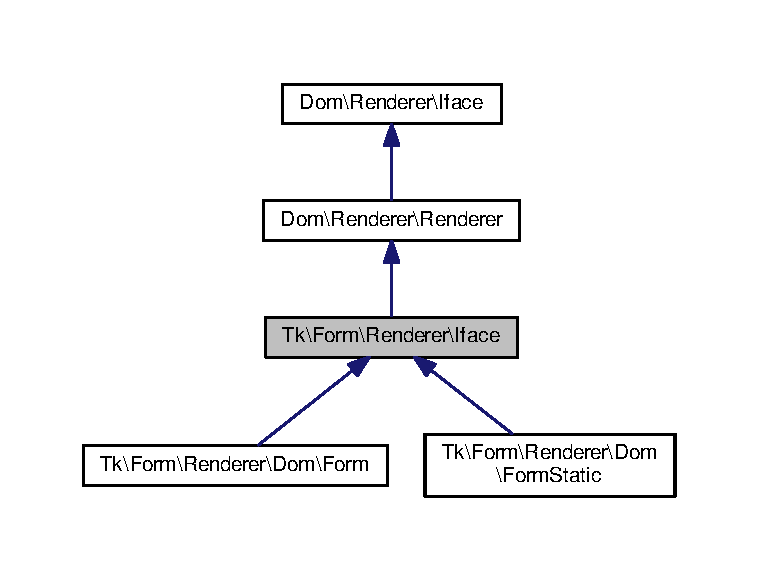
\includegraphics[width=350pt]{classTk_1_1Form_1_1Renderer_1_1Iface__inherit__graph}
\end{center}
\end{figure}
\subsection*{Public Member Functions}
\begin{DoxyCompactItemize}
\item 
\hyperlink{classTk_1_1Form_1_1Renderer_1_1Iface_a82034cf48ff5311db2ff93a1778e8ad6}{\+\_\+\+\_\+construct} (\hyperlink{classTk_1_1Form}{Form} \$form)
\item 
\hyperlink{classTk_1_1Form_1_1Renderer_1_1Iface_a3369a1b16d80d638a4dfd77ffe44a46f}{get\+Form} ()
\end{DoxyCompactItemize}
\subsection*{Protected Member Functions}
\begin{DoxyCompactItemize}
\item 
\hyperlink{classTk_1_1Form_1_1Renderer_1_1Iface_ad407035177586de22e69768a340002ed}{show\+Field} (\hyperlink{classTk_1_1Form_1_1Field_1_1Iface}{Field\textbackslash{}\+Iface} \$field)
\end{DoxyCompactItemize}
\subsection*{Protected Attributes}
\begin{DoxyCompactItemize}
\item 
\hypertarget{classTk_1_1Form_1_1Renderer_1_1Iface_a6b2f6b750d9c4f67aba60ced2178a392}{{\bfseries \$form} = null}\label{classTk_1_1Form_1_1Renderer_1_1Iface_a6b2f6b750d9c4f67aba60ced2178a392}

\end{DoxyCompactItemize}


\subsection{Detailed Description}
Class \hyperlink{classTk_1_1Form_1_1Renderer_1_1Iface}{Iface}

\begin{DoxyAuthor}{Author}
Michael Mifsud \href{mailto:info@tropotek.com}{\tt info@tropotek.\+com} \hyperlink{}{Copyright 2015 Michael Mifsud }
\end{DoxyAuthor}


\subsection{Constructor \& Destructor Documentation}
\hypertarget{classTk_1_1Form_1_1Renderer_1_1Iface_a82034cf48ff5311db2ff93a1778e8ad6}{\index{Tk\+::\+Form\+::\+Renderer\+::\+Iface@{Tk\+::\+Form\+::\+Renderer\+::\+Iface}!\+\_\+\+\_\+construct@{\+\_\+\+\_\+construct}}
\index{\+\_\+\+\_\+construct@{\+\_\+\+\_\+construct}!Tk\+::\+Form\+::\+Renderer\+::\+Iface@{Tk\+::\+Form\+::\+Renderer\+::\+Iface}}
\subsubsection[{\+\_\+\+\_\+construct}]{\setlength{\rightskip}{0pt plus 5cm}Tk\textbackslash{}\+Form\textbackslash{}\+Renderer\textbackslash{}\+Iface\+::\+\_\+\+\_\+construct (
\begin{DoxyParamCaption}
\item[{{\bf Form}}]{\$form}
\end{DoxyParamCaption}
)}}\label{classTk_1_1Form_1_1Renderer_1_1Iface_a82034cf48ff5311db2ff93a1778e8ad6}
construct


\begin{DoxyParams}[1]{Parameters}
\hyperlink{classTk_1_1Form}{Form} & {\em \$form} & \\
\hline
\end{DoxyParams}


\subsection{Member Function Documentation}
\hypertarget{classTk_1_1Form_1_1Renderer_1_1Iface_a3369a1b16d80d638a4dfd77ffe44a46f}{\index{Tk\+::\+Form\+::\+Renderer\+::\+Iface@{Tk\+::\+Form\+::\+Renderer\+::\+Iface}!get\+Form@{get\+Form}}
\index{get\+Form@{get\+Form}!Tk\+::\+Form\+::\+Renderer\+::\+Iface@{Tk\+::\+Form\+::\+Renderer\+::\+Iface}}
\subsubsection[{get\+Form}]{\setlength{\rightskip}{0pt plus 5cm}Tk\textbackslash{}\+Form\textbackslash{}\+Renderer\textbackslash{}\+Iface\+::get\+Form (
\begin{DoxyParamCaption}
{}
\end{DoxyParamCaption}
)}}\label{classTk_1_1Form_1_1Renderer_1_1Iface_a3369a1b16d80d638a4dfd77ffe44a46f}
Get the form

\begin{DoxyReturn}{Returns}
\hyperlink{classTk_1_1Form}{Form} 
\end{DoxyReturn}
\hypertarget{classTk_1_1Form_1_1Renderer_1_1Iface_ad407035177586de22e69768a340002ed}{\index{Tk\+::\+Form\+::\+Renderer\+::\+Iface@{Tk\+::\+Form\+::\+Renderer\+::\+Iface}!show\+Field@{show\+Field}}
\index{show\+Field@{show\+Field}!Tk\+::\+Form\+::\+Renderer\+::\+Iface@{Tk\+::\+Form\+::\+Renderer\+::\+Iface}}
\subsubsection[{show\+Field}]{\setlength{\rightskip}{0pt plus 5cm}Tk\textbackslash{}\+Form\textbackslash{}\+Renderer\textbackslash{}\+Iface\+::show\+Field (
\begin{DoxyParamCaption}
\item[{{\bf Field\textbackslash{}\+Iface}}]{\$field}
\end{DoxyParamCaption}
)\hspace{0.3cm}{\ttfamily [abstract]}, {\ttfamily [protected]}}}\label{classTk_1_1Form_1_1Renderer_1_1Iface_ad407035177586de22e69768a340002ed}
Render the form field values


\begin{DoxyParams}[1]{Parameters}
Field\textbackslash{}\+Iface & {\em \$field} & \\
\hline
\end{DoxyParams}
\begin{DoxyReturn}{Returns}
mixed 
\end{DoxyReturn}


The documentation for this class was generated from the following file\+:\begin{DoxyCompactItemize}
\item 
vendor/ttek/tk-\/form/\+Tk/\+Form/\+Renderer/Iface.\+php\end{DoxyCompactItemize}

\hypertarget{classDom_1_1Loader_1_1Adapter_1_1Iface}{\section{Dom\textbackslash{}Loader\textbackslash{}Adapter\textbackslash{}Iface Class Reference}
\label{classDom_1_1Loader_1_1Adapter_1_1Iface}\index{Dom\textbackslash{}\+Loader\textbackslash{}\+Adapter\textbackslash{}\+Iface@{Dom\textbackslash{}\+Loader\textbackslash{}\+Adapter\textbackslash{}\+Iface}}
}


Inheritance diagram for Dom\textbackslash{}Loader\textbackslash{}Adapter\textbackslash{}Iface\+:\nopagebreak
\begin{figure}[H]
\begin{center}
\leavevmode
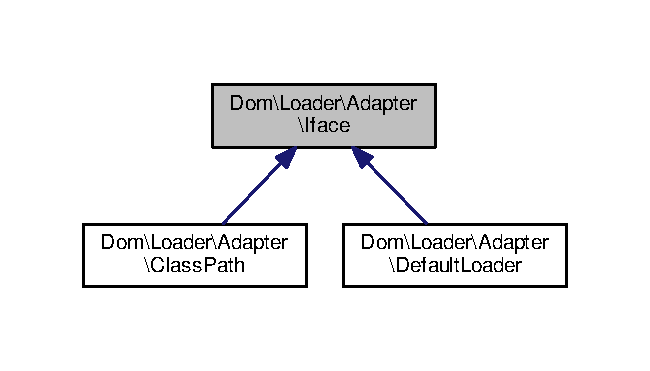
\includegraphics[width=312pt]{classDom_1_1Loader_1_1Adapter_1_1Iface__inherit__graph}
\end{center}
\end{figure}
\subsection*{Public Member Functions}
\begin{DoxyCompactItemize}
\item 
\hyperlink{classDom_1_1Loader_1_1Adapter_1_1Iface_a87c7d855de8796f3f83411590ee596bc}{load} (\$xhtml, \$class)
\item 
\hyperlink{classDom_1_1Loader_1_1Adapter_1_1Iface_a2214412ae086bb253bd7b0d5d02ef728}{load\+File} (\$path, \$class)
\item 
\hyperlink{classDom_1_1Loader_1_1Adapter_1_1Iface_af65cea996aed48e510d96e2c2b6744e4}{get\+Loader} ()
\item 
\hyperlink{classDom_1_1Loader_1_1Adapter_1_1Iface_a59953d4916b390dbb009c76667d435d6}{set\+Loader} (\$loader)
\end{DoxyCompactItemize}
\subsection*{Protected Attributes}
\begin{DoxyCompactItemize}
\item 
\hypertarget{classDom_1_1Loader_1_1Adapter_1_1Iface_a70960d6e1d569a44fcfed8138017536e}{{\bfseries \$loader} = null}\label{classDom_1_1Loader_1_1Adapter_1_1Iface_a70960d6e1d569a44fcfed8138017536e}

\end{DoxyCompactItemize}


\subsection{Detailed Description}
Class \hyperlink{classDom_1_1Loader_1_1Adapter_1_1Iface}{Iface}

\begin{DoxyAuthor}{Author}
Michael Mifsud \href{mailto:info@tropotek.com}{\tt info@tropotek.\+com} \hyperlink{}{Copyright 2015 Michael Mifsud }
\end{DoxyAuthor}


\subsection{Member Function Documentation}
\hypertarget{classDom_1_1Loader_1_1Adapter_1_1Iface_af65cea996aed48e510d96e2c2b6744e4}{\index{Dom\+::\+Loader\+::\+Adapter\+::\+Iface@{Dom\+::\+Loader\+::\+Adapter\+::\+Iface}!get\+Loader@{get\+Loader}}
\index{get\+Loader@{get\+Loader}!Dom\+::\+Loader\+::\+Adapter\+::\+Iface@{Dom\+::\+Loader\+::\+Adapter\+::\+Iface}}
\subsubsection[{get\+Loader}]{\setlength{\rightskip}{0pt plus 5cm}Dom\textbackslash{}\+Loader\textbackslash{}\+Adapter\textbackslash{}\+Iface\+::get\+Loader (
\begin{DoxyParamCaption}
{}
\end{DoxyParamCaption}
)}}\label{classDom_1_1Loader_1_1Adapter_1_1Iface_af65cea996aed48e510d96e2c2b6744e4}
\begin{DoxyReturn}{Returns}
\hyperlink{classDom_1_1Loader}{Loader} 
\end{DoxyReturn}
\hypertarget{classDom_1_1Loader_1_1Adapter_1_1Iface_a87c7d855de8796f3f83411590ee596bc}{\index{Dom\+::\+Loader\+::\+Adapter\+::\+Iface@{Dom\+::\+Loader\+::\+Adapter\+::\+Iface}!load@{load}}
\index{load@{load}!Dom\+::\+Loader\+::\+Adapter\+::\+Iface@{Dom\+::\+Loader\+::\+Adapter\+::\+Iface}}
\subsubsection[{load}]{\setlength{\rightskip}{0pt plus 5cm}Dom\textbackslash{}\+Loader\textbackslash{}\+Adapter\textbackslash{}\+Iface\+::load (
\begin{DoxyParamCaption}
\item[{}]{\$xhtml, }
\item[{}]{\$class}
\end{DoxyParamCaption}
)\hspace{0.3cm}{\ttfamily [abstract]}}}\label{classDom_1_1Loader_1_1Adapter_1_1Iface_a87c7d855de8796f3f83411590ee596bc}
Load an xml/xhtml strings


\begin{DoxyParams}{Parameters}
{\em \$xhtml} & \\
\hline
{\em \$class} & \\
\hline
\end{DoxyParams}
\begin{DoxyReturn}{Returns}

\end{DoxyReturn}
\hypertarget{classDom_1_1Loader_1_1Adapter_1_1Iface_a2214412ae086bb253bd7b0d5d02ef728}{\index{Dom\+::\+Loader\+::\+Adapter\+::\+Iface@{Dom\+::\+Loader\+::\+Adapter\+::\+Iface}!load\+File@{load\+File}}
\index{load\+File@{load\+File}!Dom\+::\+Loader\+::\+Adapter\+::\+Iface@{Dom\+::\+Loader\+::\+Adapter\+::\+Iface}}
\subsubsection[{load\+File}]{\setlength{\rightskip}{0pt plus 5cm}Dom\textbackslash{}\+Loader\textbackslash{}\+Adapter\textbackslash{}\+Iface\+::load\+File (
\begin{DoxyParamCaption}
\item[{}]{\$path, }
\item[{}]{\$class}
\end{DoxyParamCaption}
)\hspace{0.3cm}{\ttfamily [abstract]}}}\label{classDom_1_1Loader_1_1Adapter_1_1Iface_a2214412ae086bb253bd7b0d5d02ef728}
Load an xml/xhtml file


\begin{DoxyParams}{Parameters}
{\em \$path} & \\
\hline
{\em \$class} & \\
\hline
\end{DoxyParams}
\begin{DoxyReturn}{Returns}

\end{DoxyReturn}
\hypertarget{classDom_1_1Loader_1_1Adapter_1_1Iface_a59953d4916b390dbb009c76667d435d6}{\index{Dom\+::\+Loader\+::\+Adapter\+::\+Iface@{Dom\+::\+Loader\+::\+Adapter\+::\+Iface}!set\+Loader@{set\+Loader}}
\index{set\+Loader@{set\+Loader}!Dom\+::\+Loader\+::\+Adapter\+::\+Iface@{Dom\+::\+Loader\+::\+Adapter\+::\+Iface}}
\subsubsection[{set\+Loader}]{\setlength{\rightskip}{0pt plus 5cm}Dom\textbackslash{}\+Loader\textbackslash{}\+Adapter\textbackslash{}\+Iface\+::set\+Loader (
\begin{DoxyParamCaption}
\item[{}]{\$loader}
\end{DoxyParamCaption}
)}}\label{classDom_1_1Loader_1_1Adapter_1_1Iface_a59953d4916b390dbb009c76667d435d6}

\begin{DoxyParams}[1]{Parameters}
\hyperlink{classDom_1_1Loader}{Loader} & {\em \$loader} & \\
\hline
\end{DoxyParams}


The documentation for this class was generated from the following file\+:\begin{DoxyCompactItemize}
\item 
vendor/ttek/tk-\/domtemplate/\+Dom/\+Loader/\+Adapter/Iface.\+php\end{DoxyCompactItemize}

\hypertarget{classTk_1_1Dom_1_1Modifier_1_1Filter_1_1Iface}{\section{Tk\textbackslash{}Dom\textbackslash{}Modifier\textbackslash{}Filter\textbackslash{}Iface Class Reference}
\label{classTk_1_1Dom_1_1Modifier_1_1Filter_1_1Iface}\index{Tk\textbackslash{}\+Dom\textbackslash{}\+Modifier\textbackslash{}\+Filter\textbackslash{}\+Iface@{Tk\textbackslash{}\+Dom\textbackslash{}\+Modifier\textbackslash{}\+Filter\textbackslash{}\+Iface}}
}


Inheritance diagram for Tk\textbackslash{}Dom\textbackslash{}Modifier\textbackslash{}Filter\textbackslash{}Iface\+:\nopagebreak
\begin{figure}[H]
\begin{center}
\leavevmode
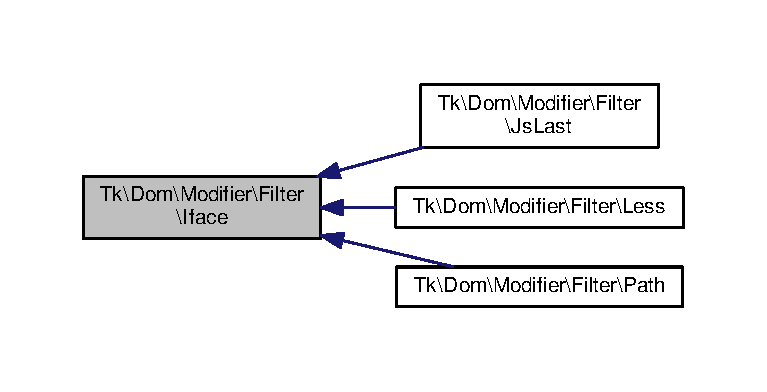
\includegraphics[width=350pt]{classTk_1_1Dom_1_1Modifier_1_1Filter_1_1Iface__inherit__graph}
\end{center}
\end{figure}
\subsection*{Public Member Functions}
\begin{DoxyCompactItemize}
\item 
\hyperlink{classTk_1_1Dom_1_1Modifier_1_1Filter_1_1Iface_ad7ca6a2844adf778d334d22dc1001785}{set\+Dom\+Modifier} (\hyperlink{classTk_1_1Dom_1_1Modifier_1_1Modifier}{Modifier} \$dm)
\item 
\hyperlink{classTk_1_1Dom_1_1Modifier_1_1Filter_1_1Iface_a9cb0edc59c7299b123f443cd8a9e8caf}{set\+Enable} (\$b)
\item 
\hyperlink{classTk_1_1Dom_1_1Modifier_1_1Filter_1_1Iface_af2361ea31b54e2ed74feff865423e145}{is\+Enabled} ()
\item 
\hyperlink{classTk_1_1Dom_1_1Modifier_1_1Filter_1_1Iface_a3fb21a70a41f94cfea4dce38bd4e13fc}{init} (\$doc)
\item 
\hyperlink{classTk_1_1Dom_1_1Modifier_1_1Filter_1_1Iface_a05cb828e17a22aa923f36bfc81c41335}{post\+Traverse} (\$doc)
\item 
\hyperlink{classTk_1_1Dom_1_1Modifier_1_1Filter_1_1Iface_a987e5c74d9365b6cd1be7a9a5b768bbf}{execute\+Node} (\textbackslash{}D\+O\+M\+Element \$node)
\end{DoxyCompactItemize}
\subsection*{Protected Attributes}
\begin{DoxyCompactItemize}
\item 
\hypertarget{classTk_1_1Dom_1_1Modifier_1_1Filter_1_1Iface_ac1b5e6d70848ef34103f976cc0046c46}{{\bfseries \$dom\+Modifier} = null}\label{classTk_1_1Dom_1_1Modifier_1_1Filter_1_1Iface_ac1b5e6d70848ef34103f976cc0046c46}

\item 
\hypertarget{classTk_1_1Dom_1_1Modifier_1_1Filter_1_1Iface_a3aa2aa98bdbb5a73ce1c51d9647b60c5}{{\bfseries \$enabled} = true}\label{classTk_1_1Dom_1_1Modifier_1_1Filter_1_1Iface_a3aa2aa98bdbb5a73ce1c51d9647b60c5}

\end{DoxyCompactItemize}


\subsection{Detailed Description}
The interface for all Dom\+Modifier filter objects

\begin{DoxyAuthor}{Author}
Michael Mifsud \href{mailto:info@tropotek.com}{\tt info@tropotek.\+com} \hyperlink{}{Copyright 2007 Michael Mifsud }
\end{DoxyAuthor}


\subsection{Member Function Documentation}
\hypertarget{classTk_1_1Dom_1_1Modifier_1_1Filter_1_1Iface_a987e5c74d9365b6cd1be7a9a5b768bbf}{\index{Tk\+::\+Dom\+::\+Modifier\+::\+Filter\+::\+Iface@{Tk\+::\+Dom\+::\+Modifier\+::\+Filter\+::\+Iface}!execute\+Node@{execute\+Node}}
\index{execute\+Node@{execute\+Node}!Tk\+::\+Dom\+::\+Modifier\+::\+Filter\+::\+Iface@{Tk\+::\+Dom\+::\+Modifier\+::\+Filter\+::\+Iface}}
\subsubsection[{execute\+Node}]{\setlength{\rightskip}{0pt plus 5cm}Tk\textbackslash{}\+Dom\textbackslash{}\+Modifier\textbackslash{}\+Filter\textbackslash{}\+Iface\+::execute\+Node (
\begin{DoxyParamCaption}
\item[{\textbackslash{}D\+O\+M\+Element}]{\$node}
\end{DoxyParamCaption}
)\hspace{0.3cm}{\ttfamily [abstract]}}}\label{classTk_1_1Dom_1_1Modifier_1_1Filter_1_1Iface_a987e5c74d9365b6cd1be7a9a5b768bbf}
The code to perform any modification to the node goes here.


\begin{DoxyParams}[1]{Parameters}
\textbackslash{}\+D\+O\+M\+Element & {\em \$node} & \\
\hline
\end{DoxyParams}
\hypertarget{classTk_1_1Dom_1_1Modifier_1_1Filter_1_1Iface_a3fb21a70a41f94cfea4dce38bd4e13fc}{\index{Tk\+::\+Dom\+::\+Modifier\+::\+Filter\+::\+Iface@{Tk\+::\+Dom\+::\+Modifier\+::\+Filter\+::\+Iface}!init@{init}}
\index{init@{init}!Tk\+::\+Dom\+::\+Modifier\+::\+Filter\+::\+Iface@{Tk\+::\+Dom\+::\+Modifier\+::\+Filter\+::\+Iface}}
\subsubsection[{init}]{\setlength{\rightskip}{0pt plus 5cm}Tk\textbackslash{}\+Dom\textbackslash{}\+Modifier\textbackslash{}\+Filter\textbackslash{}\+Iface\+::init (
\begin{DoxyParamCaption}
\item[{}]{\$doc}
\end{DoxyParamCaption}
)\hspace{0.3cm}{\ttfamily [abstract]}}}\label{classTk_1_1Dom_1_1Modifier_1_1Filter_1_1Iface_a3fb21a70a41f94cfea4dce38bd4e13fc}
pre init the front controller


\begin{DoxyParams}[1]{Parameters}
\textbackslash{}\+D\+O\+M\+Document & {\em \$doc} & \\
\hline
\end{DoxyParams}
\hypertarget{classTk_1_1Dom_1_1Modifier_1_1Filter_1_1Iface_af2361ea31b54e2ed74feff865423e145}{\index{Tk\+::\+Dom\+::\+Modifier\+::\+Filter\+::\+Iface@{Tk\+::\+Dom\+::\+Modifier\+::\+Filter\+::\+Iface}!is\+Enabled@{is\+Enabled}}
\index{is\+Enabled@{is\+Enabled}!Tk\+::\+Dom\+::\+Modifier\+::\+Filter\+::\+Iface@{Tk\+::\+Dom\+::\+Modifier\+::\+Filter\+::\+Iface}}
\subsubsection[{is\+Enabled}]{\setlength{\rightskip}{0pt plus 5cm}Tk\textbackslash{}\+Dom\textbackslash{}\+Modifier\textbackslash{}\+Filter\textbackslash{}\+Iface\+::is\+Enabled (
\begin{DoxyParamCaption}
{}
\end{DoxyParamCaption}
)}}\label{classTk_1_1Dom_1_1Modifier_1_1Filter_1_1Iface_af2361ea31b54e2ed74feff865423e145}
Get the enabled status.

\begin{DoxyReturn}{Returns}
bool 
\end{DoxyReturn}
\hypertarget{classTk_1_1Dom_1_1Modifier_1_1Filter_1_1Iface_a05cb828e17a22aa923f36bfc81c41335}{\index{Tk\+::\+Dom\+::\+Modifier\+::\+Filter\+::\+Iface@{Tk\+::\+Dom\+::\+Modifier\+::\+Filter\+::\+Iface}!post\+Traverse@{post\+Traverse}}
\index{post\+Traverse@{post\+Traverse}!Tk\+::\+Dom\+::\+Modifier\+::\+Filter\+::\+Iface@{Tk\+::\+Dom\+::\+Modifier\+::\+Filter\+::\+Iface}}
\subsubsection[{post\+Traverse}]{\setlength{\rightskip}{0pt plus 5cm}Tk\textbackslash{}\+Dom\textbackslash{}\+Modifier\textbackslash{}\+Filter\textbackslash{}\+Iface\+::post\+Traverse (
\begin{DoxyParamCaption}
\item[{}]{\$doc}
\end{DoxyParamCaption}
)}}\label{classTk_1_1Dom_1_1Modifier_1_1Filter_1_1Iface_a05cb828e17a22aa923f36bfc81c41335}
called after D\+O\+M tree is traversed


\begin{DoxyParams}[1]{Parameters}
\textbackslash{}\+D\+O\+M\+Document & {\em \$doc} & \\
\hline
\end{DoxyParams}
\hypertarget{classTk_1_1Dom_1_1Modifier_1_1Filter_1_1Iface_ad7ca6a2844adf778d334d22dc1001785}{\index{Tk\+::\+Dom\+::\+Modifier\+::\+Filter\+::\+Iface@{Tk\+::\+Dom\+::\+Modifier\+::\+Filter\+::\+Iface}!set\+Dom\+Modifier@{set\+Dom\+Modifier}}
\index{set\+Dom\+Modifier@{set\+Dom\+Modifier}!Tk\+::\+Dom\+::\+Modifier\+::\+Filter\+::\+Iface@{Tk\+::\+Dom\+::\+Modifier\+::\+Filter\+::\+Iface}}
\subsubsection[{set\+Dom\+Modifier}]{\setlength{\rightskip}{0pt plus 5cm}Tk\textbackslash{}\+Dom\textbackslash{}\+Modifier\textbackslash{}\+Filter\textbackslash{}\+Iface\+::set\+Dom\+Modifier (
\begin{DoxyParamCaption}
\item[{{\bf Modifier}}]{\$dm}
\end{DoxyParamCaption}
)}}\label{classTk_1_1Dom_1_1Modifier_1_1Filter_1_1Iface_ad7ca6a2844adf778d334d22dc1001785}
Set Dom \hyperlink{classTk_1_1Dom_1_1Modifier_1_1Modifier}{Modifier}


\begin{DoxyParams}[1]{Parameters}
\hyperlink{classTk_1_1Dom_1_1Modifier_1_1Modifier}{Modifier} & {\em \$dm} & \\
\hline
\end{DoxyParams}
\hypertarget{classTk_1_1Dom_1_1Modifier_1_1Filter_1_1Iface_a9cb0edc59c7299b123f443cd8a9e8caf}{\index{Tk\+::\+Dom\+::\+Modifier\+::\+Filter\+::\+Iface@{Tk\+::\+Dom\+::\+Modifier\+::\+Filter\+::\+Iface}!set\+Enable@{set\+Enable}}
\index{set\+Enable@{set\+Enable}!Tk\+::\+Dom\+::\+Modifier\+::\+Filter\+::\+Iface@{Tk\+::\+Dom\+::\+Modifier\+::\+Filter\+::\+Iface}}
\subsubsection[{set\+Enable}]{\setlength{\rightskip}{0pt plus 5cm}Tk\textbackslash{}\+Dom\textbackslash{}\+Modifier\textbackslash{}\+Filter\textbackslash{}\+Iface\+::set\+Enable (
\begin{DoxyParamCaption}
\item[{}]{\$b}
\end{DoxyParamCaption}
)}}\label{classTk_1_1Dom_1_1Modifier_1_1Filter_1_1Iface_a9cb0edc59c7299b123f443cd8a9e8caf}
Set the enabled state of the object


\begin{DoxyParams}[1]{Parameters}
bool & {\em \$b} & \\
\hline
\end{DoxyParams}


The documentation for this class was generated from the following file\+:\begin{DoxyCompactItemize}
\item 
vendor/ttek/tk-\/framework/\+Tk/\+Dom/\+Modifier/\+Filter/Iface.\+php\end{DoxyCompactItemize}

\hypertarget{interfaceDom_1_1Renderer_1_1Iface}{\section{Dom\textbackslash{}Renderer\textbackslash{}Iface Interface Reference}
\label{interfaceDom_1_1Renderer_1_1Iface}\index{Dom\textbackslash{}\+Renderer\textbackslash{}\+Iface@{Dom\textbackslash{}\+Renderer\textbackslash{}\+Iface}}
}


Inheritance diagram for Dom\textbackslash{}Renderer\textbackslash{}Iface\+:\nopagebreak
\begin{figure}[H]
\begin{center}
\leavevmode
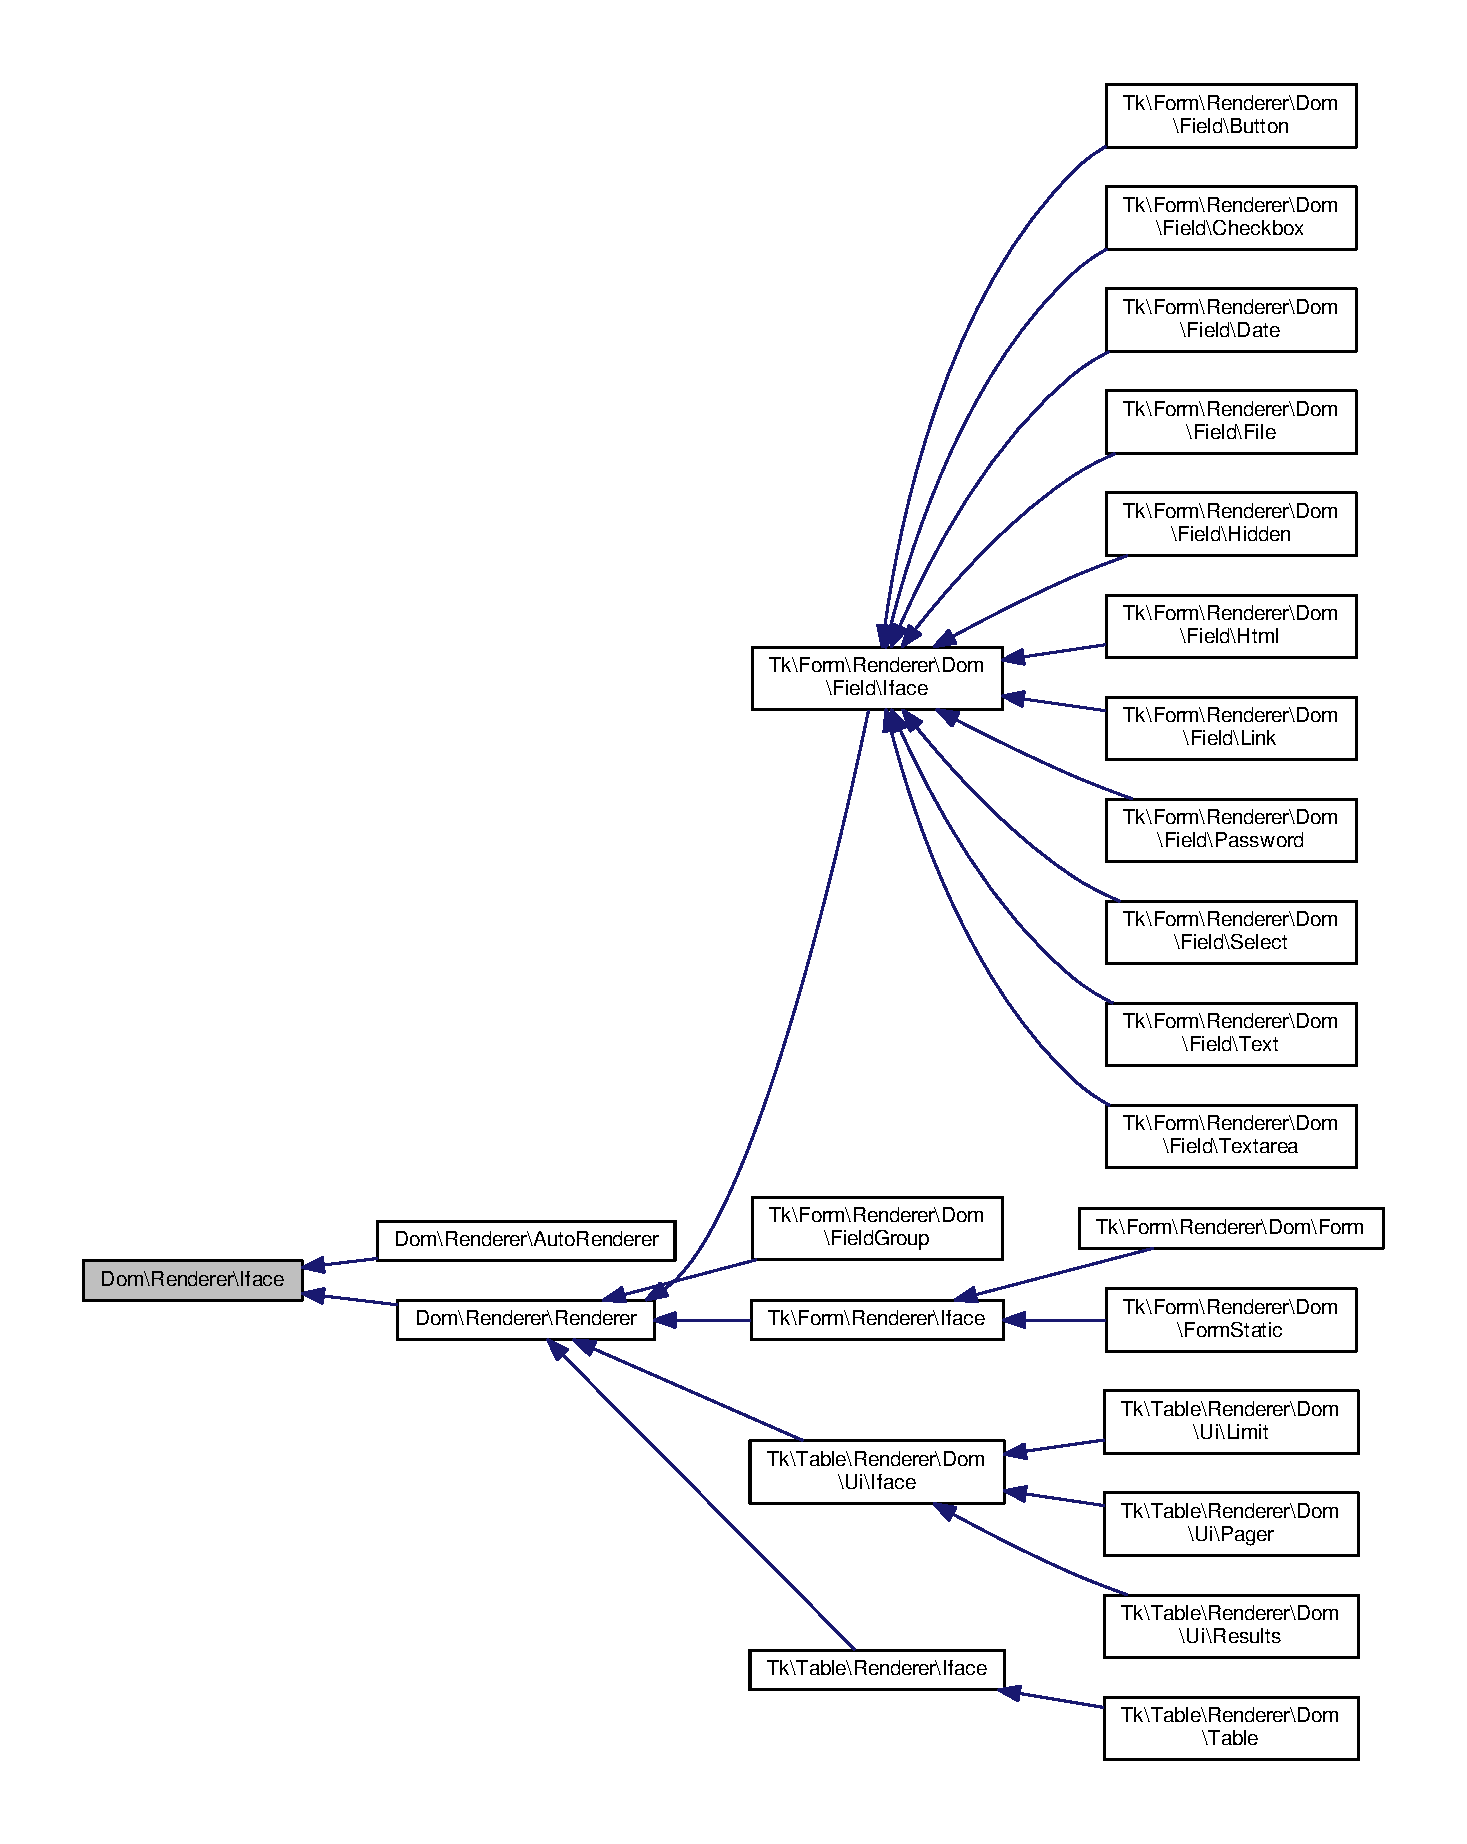
\includegraphics[width=350pt]{interfaceDom_1_1Renderer_1_1Iface__inherit__graph}
\end{center}
\end{figure}
\subsection*{Public Member Functions}
\begin{DoxyCompactItemize}
\item 
\hyperlink{interfaceDom_1_1Renderer_1_1Iface_a79a0ba41fb6714d69156891d6326bd33}{show} ()
\item 
\hyperlink{interfaceDom_1_1Renderer_1_1Iface_ad24995320dbbbd8a1796c1d13518012c}{get\+Template} ()
\item 
\hyperlink{interfaceDom_1_1Renderer_1_1Iface_a6e4c7ff3f90a9b1a26bc08bf6e1408d6}{set\+Template} (\$template)
\end{DoxyCompactItemize}


\subsection{Detailed Description}
\hyperlink{classDom_1_1Template}{Template} Bootstrap interface

\begin{DoxyAuthor}{Author}
Michael Mifsud \href{mailto:info@tropotek.com}{\tt info@tropotek.\+com} \hyperlink{}{Copyright 2007 Michael Mifsud }
\end{DoxyAuthor}


\subsection{Member Function Documentation}
\hypertarget{interfaceDom_1_1Renderer_1_1Iface_ad24995320dbbbd8a1796c1d13518012c}{\index{Dom\+::\+Renderer\+::\+Iface@{Dom\+::\+Renderer\+::\+Iface}!get\+Template@{get\+Template}}
\index{get\+Template@{get\+Template}!Dom\+::\+Renderer\+::\+Iface@{Dom\+::\+Renderer\+::\+Iface}}
\subsubsection[{get\+Template}]{\setlength{\rightskip}{0pt plus 5cm}Dom\textbackslash{}\+Renderer\textbackslash{}\+Iface\+::get\+Template (
\begin{DoxyParamCaption}
{}
\end{DoxyParamCaption}
)}}\label{interfaceDom_1_1Renderer_1_1Iface_ad24995320dbbbd8a1796c1d13518012c}
Get the 

\begin{DoxyReturn}{Returns}

\end{DoxyReturn}


Implemented in \hyperlink{classDom_1_1Renderer_1_1AutoRenderer_a7c6ac2e26298cf2a8be324f6e44056cf}{Dom\textbackslash{}\+Renderer\textbackslash{}\+Auto\+Renderer}, and \hyperlink{classDom_1_1Renderer_1_1Renderer_a103355306876ef3a764911483c0a09ec}{Dom\textbackslash{}\+Renderer\textbackslash{}\+Renderer}.

\hypertarget{interfaceDom_1_1Renderer_1_1Iface_a6e4c7ff3f90a9b1a26bc08bf6e1408d6}{\index{Dom\+::\+Renderer\+::\+Iface@{Dom\+::\+Renderer\+::\+Iface}!set\+Template@{set\+Template}}
\index{set\+Template@{set\+Template}!Dom\+::\+Renderer\+::\+Iface@{Dom\+::\+Renderer\+::\+Iface}}
\subsubsection[{set\+Template}]{\setlength{\rightskip}{0pt plus 5cm}Dom\textbackslash{}\+Renderer\textbackslash{}\+Iface\+::set\+Template (
\begin{DoxyParamCaption}
\item[{}]{\$template}
\end{DoxyParamCaption}
)}}\label{interfaceDom_1_1Renderer_1_1Iface_a6e4c7ff3f90a9b1a26bc08bf6e1408d6}
Set the 


\begin{DoxyParams}[1]{Parameters}
\textbackslash{}\+Dom\textbackslash{}\+Template & {\em \$template} & \\
\hline
\end{DoxyParams}


Implemented in \hyperlink{classDom_1_1Renderer_1_1AutoRenderer_a8c34c043c962f53241f825579839750c}{Dom\textbackslash{}\+Renderer\textbackslash{}\+Auto\+Renderer}, and \hyperlink{classDom_1_1Renderer_1_1Renderer_a3c9549e694a794e55d920da28570397f}{Dom\textbackslash{}\+Renderer\textbackslash{}\+Renderer}.

\hypertarget{interfaceDom_1_1Renderer_1_1Iface_a79a0ba41fb6714d69156891d6326bd33}{\index{Dom\+::\+Renderer\+::\+Iface@{Dom\+::\+Renderer\+::\+Iface}!show@{show}}
\index{show@{show}!Dom\+::\+Renderer\+::\+Iface@{Dom\+::\+Renderer\+::\+Iface}}
\subsubsection[{show}]{\setlength{\rightskip}{0pt plus 5cm}Dom\textbackslash{}\+Renderer\textbackslash{}\+Iface\+::show (
\begin{DoxyParamCaption}
{}
\end{DoxyParamCaption}
)}}\label{interfaceDom_1_1Renderer_1_1Iface_a79a0ba41fb6714d69156891d6326bd33}
Execute the renderer. The returned object can be anything that you need to render the output.

\begin{DoxyReturn}{Returns}
mixed 
\end{DoxyReturn}


Implemented in \hyperlink{classTk_1_1Table_1_1Renderer_1_1Dom_1_1Ui_1_1Pager_ae40067db74fa55f76345f0ba9eef3f56}{Tk\textbackslash{}\+Table\textbackslash{}\+Renderer\textbackslash{}\+Dom\textbackslash{}\+Ui\textbackslash{}\+Pager}, \hyperlink{classDom_1_1Renderer_1_1AutoRenderer_a71ad96ed156aa79d45058b3bf372e73d}{Dom\textbackslash{}\+Renderer\textbackslash{}\+Auto\+Renderer}, \hyperlink{classTk_1_1Table_1_1Renderer_1_1Dom_1_1Table_aeef7366176a250dbee759e9ff78062ee}{Tk\textbackslash{}\+Table\textbackslash{}\+Renderer\textbackslash{}\+Dom\textbackslash{}\+Table}, \hyperlink{classTk_1_1Table_1_1Renderer_1_1Dom_1_1Ui_1_1Results_a6cb4921fdb6a62b96a35d80c780df122}{Tk\textbackslash{}\+Table\textbackslash{}\+Renderer\textbackslash{}\+Dom\textbackslash{}\+Ui\textbackslash{}\+Results}, \hyperlink{classTk_1_1Form_1_1Renderer_1_1Dom_1_1FormStatic_a26fa1ebf33c3504b3f599adf1070e043}{Tk\textbackslash{}\+Form\textbackslash{}\+Renderer\textbackslash{}\+Dom\textbackslash{}\+Form\+Static}, \hyperlink{classTk_1_1Form_1_1Renderer_1_1Dom_1_1FieldGroup_afd18726c000171d11abfd6044d1e3b01}{Tk\textbackslash{}\+Form\textbackslash{}\+Renderer\textbackslash{}\+Dom\textbackslash{}\+Field\+Group}, \hyperlink{classTk_1_1Table_1_1Renderer_1_1Dom_1_1Ui_1_1Limit_a7afabb245a6701c7ebd6f35fa2ffe704}{Tk\textbackslash{}\+Table\textbackslash{}\+Renderer\textbackslash{}\+Dom\textbackslash{}\+Ui\textbackslash{}\+Limit}, \hyperlink{classTk_1_1Form_1_1Renderer_1_1Dom_1_1Field_1_1Iface_a77359df4fad53376f97b6a192410c54b}{Tk\textbackslash{}\+Form\textbackslash{}\+Renderer\textbackslash{}\+Dom\textbackslash{}\+Field\textbackslash{}\+Iface}, \hyperlink{classTk_1_1Form_1_1Renderer_1_1Dom_1_1Form_a2b67b6b33d1cffdffc04010dad181b93}{Tk\textbackslash{}\+Form\textbackslash{}\+Renderer\textbackslash{}\+Dom\textbackslash{}\+Form}, \hyperlink{classTk_1_1Form_1_1Renderer_1_1Dom_1_1Field_1_1File_adc2d7a4f70c408469660a243ec791acc}{Tk\textbackslash{}\+Form\textbackslash{}\+Renderer\textbackslash{}\+Dom\textbackslash{}\+Field\textbackslash{}\+File}, \hyperlink{classTk_1_1Form_1_1Renderer_1_1Dom_1_1Field_1_1Hidden_a482c59511558e1e4bdf83d943fc2800d}{Tk\textbackslash{}\+Form\textbackslash{}\+Renderer\textbackslash{}\+Dom\textbackslash{}\+Field\textbackslash{}\+Hidden}, \hyperlink{classTk_1_1Form_1_1Renderer_1_1Dom_1_1Field_1_1Button_a7fb360221146282195b769db9ef4d814}{Tk\textbackslash{}\+Form\textbackslash{}\+Renderer\textbackslash{}\+Dom\textbackslash{}\+Field\textbackslash{}\+Button}, and \hyperlink{classTk_1_1Form_1_1Renderer_1_1Dom_1_1Field_1_1Link_a30a4fe16a4d31b92bcc6d1cdb6505d22}{Tk\textbackslash{}\+Form\textbackslash{}\+Renderer\textbackslash{}\+Dom\textbackslash{}\+Field\textbackslash{}\+Link}.



The documentation for this interface was generated from the following file\+:\begin{DoxyCompactItemize}
\item 
vendor/ttek/tk-\/domtemplate/\+Dom/\+Renderer/Iface.\+php\end{DoxyCompactItemize}

\hypertarget{classTk_1_1Form_1_1Renderer_1_1Dom_1_1Field_1_1Iface}{\section{Tk\textbackslash{}Form\textbackslash{}Renderer\textbackslash{}Dom\textbackslash{}Field\textbackslash{}Iface Class Reference}
\label{classTk_1_1Form_1_1Renderer_1_1Dom_1_1Field_1_1Iface}\index{Tk\textbackslash{}\+Form\textbackslash{}\+Renderer\textbackslash{}\+Dom\textbackslash{}\+Field\textbackslash{}\+Iface@{Tk\textbackslash{}\+Form\textbackslash{}\+Renderer\textbackslash{}\+Dom\textbackslash{}\+Field\textbackslash{}\+Iface}}
}


Inheritance diagram for Tk\textbackslash{}Form\textbackslash{}Renderer\textbackslash{}Dom\textbackslash{}Field\textbackslash{}Iface\+:\nopagebreak
\begin{figure}[H]
\begin{center}
\leavevmode
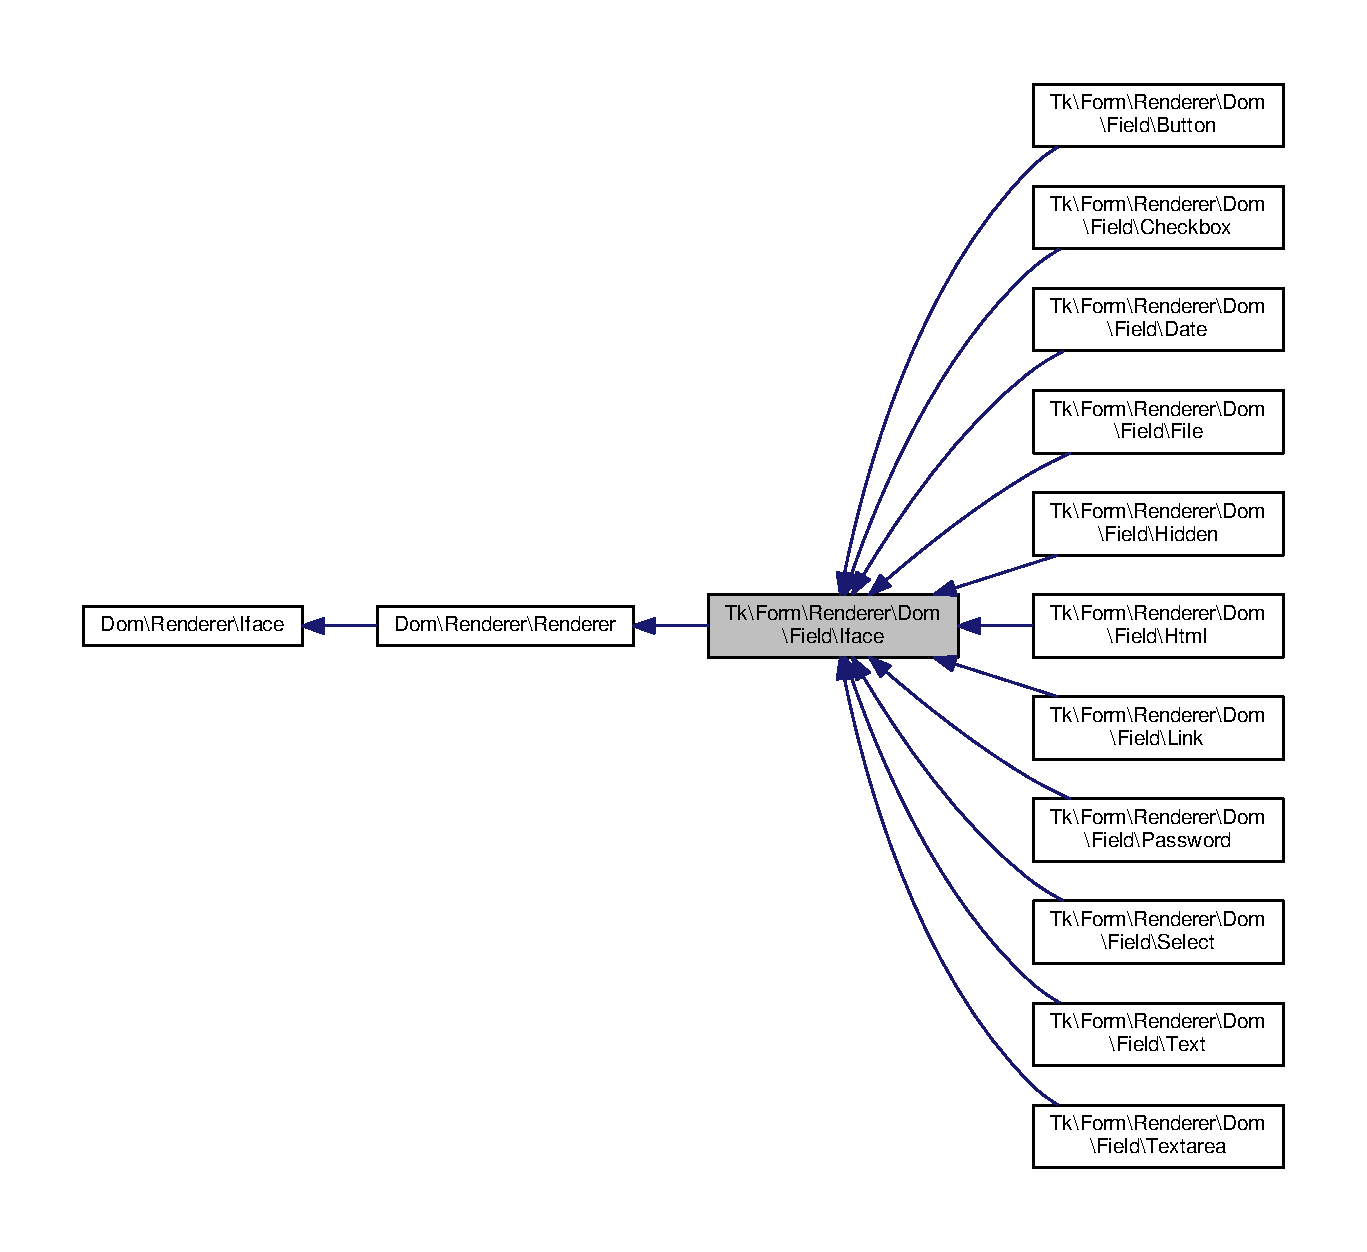
\includegraphics[width=350pt]{classTk_1_1Form_1_1Renderer_1_1Dom_1_1Field_1_1Iface__inherit__graph}
\end{center}
\end{figure}
\subsection*{Public Member Functions}
\begin{DoxyCompactItemize}
\item 
\hyperlink{classTk_1_1Form_1_1Renderer_1_1Dom_1_1Field_1_1Iface_ae9df61fb81750b399bf0c27b1ca5d4f1}{\+\_\+\+\_\+construct} (\hyperlink{classTk_1_1Form_1_1Renderer_1_1Dom_1_1Field_1_1Iface}{Field\textbackslash{}\+Iface} \$field)
\item 
\hyperlink{classTk_1_1Form_1_1Renderer_1_1Dom_1_1Field_1_1Iface_ae4a35c133973445da3324bf3b7ce9fab}{get\+Field} ()
\item 
\hyperlink{classTk_1_1Form_1_1Renderer_1_1Dom_1_1Field_1_1Iface_a77359df4fad53376f97b6a192410c54b}{show} ()
\item 
\hyperlink{classTk_1_1Form_1_1Renderer_1_1Dom_1_1Field_1_1Iface_ab060b02a360a0dfbdbff8d883a4d1b0c}{show\+Element} ()
\end{DoxyCompactItemize}
\subsection*{Protected Attributes}
\begin{DoxyCompactItemize}
\item 
\hypertarget{classTk_1_1Form_1_1Renderer_1_1Dom_1_1Field_1_1Iface_ae910ec533af54cf1a3fd87b62372db7e}{{\bfseries \$field} = null}\label{classTk_1_1Form_1_1Renderer_1_1Dom_1_1Field_1_1Iface_ae910ec533af54cf1a3fd87b62372db7e}

\end{DoxyCompactItemize}


\subsection{Detailed Description}
Field D\+O\+M renderer interface

\begin{DoxyAuthor}{Author}
Michael Mifsud \href{mailto:info@tropotek.com}{\tt info@tropotek.\+com} \hyperlink{}{Copyright 2015 Michael Mifsud }
\end{DoxyAuthor}


\subsection{Constructor \& Destructor Documentation}
\hypertarget{classTk_1_1Form_1_1Renderer_1_1Dom_1_1Field_1_1Iface_ae9df61fb81750b399bf0c27b1ca5d4f1}{\index{Tk\+::\+Form\+::\+Renderer\+::\+Dom\+::\+Field\+::\+Iface@{Tk\+::\+Form\+::\+Renderer\+::\+Dom\+::\+Field\+::\+Iface}!\+\_\+\+\_\+construct@{\+\_\+\+\_\+construct}}
\index{\+\_\+\+\_\+construct@{\+\_\+\+\_\+construct}!Tk\+::\+Form\+::\+Renderer\+::\+Dom\+::\+Field\+::\+Iface@{Tk\+::\+Form\+::\+Renderer\+::\+Dom\+::\+Field\+::\+Iface}}
\subsubsection[{\+\_\+\+\_\+construct}]{\setlength{\rightskip}{0pt plus 5cm}Tk\textbackslash{}\+Form\textbackslash{}\+Renderer\textbackslash{}\+Dom\textbackslash{}\+Field\textbackslash{}\+Iface\+::\+\_\+\+\_\+construct (
\begin{DoxyParamCaption}
\item[{{\bf Field\textbackslash{}\+Iface}}]{\$field}
\end{DoxyParamCaption}
)}}\label{classTk_1_1Form_1_1Renderer_1_1Dom_1_1Field_1_1Iface_ae9df61fb81750b399bf0c27b1ca5d4f1}
\+\_\+\+\_\+construct


\begin{DoxyParams}[1]{Parameters}
Field\textbackslash{}\+Iface & {\em \$field} & \\
\hline
\end{DoxyParams}


\subsection{Member Function Documentation}
\hypertarget{classTk_1_1Form_1_1Renderer_1_1Dom_1_1Field_1_1Iface_ae4a35c133973445da3324bf3b7ce9fab}{\index{Tk\+::\+Form\+::\+Renderer\+::\+Dom\+::\+Field\+::\+Iface@{Tk\+::\+Form\+::\+Renderer\+::\+Dom\+::\+Field\+::\+Iface}!get\+Field@{get\+Field}}
\index{get\+Field@{get\+Field}!Tk\+::\+Form\+::\+Renderer\+::\+Dom\+::\+Field\+::\+Iface@{Tk\+::\+Form\+::\+Renderer\+::\+Dom\+::\+Field\+::\+Iface}}
\subsubsection[{get\+Field}]{\setlength{\rightskip}{0pt plus 5cm}Tk\textbackslash{}\+Form\textbackslash{}\+Renderer\textbackslash{}\+Dom\textbackslash{}\+Field\textbackslash{}\+Iface\+::get\+Field (
\begin{DoxyParamCaption}
{}
\end{DoxyParamCaption}
)}}\label{classTk_1_1Form_1_1Renderer_1_1Dom_1_1Field_1_1Iface_ae4a35c133973445da3324bf3b7ce9fab}
\begin{DoxyReturn}{Returns}
Field 
\end{DoxyReturn}
\hypertarget{classTk_1_1Form_1_1Renderer_1_1Dom_1_1Field_1_1Iface_a77359df4fad53376f97b6a192410c54b}{\index{Tk\+::\+Form\+::\+Renderer\+::\+Dom\+::\+Field\+::\+Iface@{Tk\+::\+Form\+::\+Renderer\+::\+Dom\+::\+Field\+::\+Iface}!show@{show}}
\index{show@{show}!Tk\+::\+Form\+::\+Renderer\+::\+Dom\+::\+Field\+::\+Iface@{Tk\+::\+Form\+::\+Renderer\+::\+Dom\+::\+Field\+::\+Iface}}
\subsubsection[{show}]{\setlength{\rightskip}{0pt plus 5cm}Tk\textbackslash{}\+Form\textbackslash{}\+Renderer\textbackslash{}\+Dom\textbackslash{}\+Field\textbackslash{}\+Iface\+::show (
\begin{DoxyParamCaption}
{}
\end{DoxyParamCaption}
)}}\label{classTk_1_1Form_1_1Renderer_1_1Dom_1_1Field_1_1Iface_a77359df4fad53376f97b6a192410c54b}
Render the field 

Implements \hyperlink{interfaceDom_1_1Renderer_1_1Iface_a79a0ba41fb6714d69156891d6326bd33}{Dom\textbackslash{}\+Renderer\textbackslash{}\+Iface}.

\hypertarget{classTk_1_1Form_1_1Renderer_1_1Dom_1_1Field_1_1Iface_ab060b02a360a0dfbdbff8d883a4d1b0c}{\index{Tk\+::\+Form\+::\+Renderer\+::\+Dom\+::\+Field\+::\+Iface@{Tk\+::\+Form\+::\+Renderer\+::\+Dom\+::\+Field\+::\+Iface}!show\+Element@{show\+Element}}
\index{show\+Element@{show\+Element}!Tk\+::\+Form\+::\+Renderer\+::\+Dom\+::\+Field\+::\+Iface@{Tk\+::\+Form\+::\+Renderer\+::\+Dom\+::\+Field\+::\+Iface}}
\subsubsection[{show\+Element}]{\setlength{\rightskip}{0pt plus 5cm}Tk\textbackslash{}\+Form\textbackslash{}\+Renderer\textbackslash{}\+Dom\textbackslash{}\+Field\textbackslash{}\+Iface\+::show\+Element (
\begin{DoxyParamCaption}
{}
\end{DoxyParamCaption}
)}}\label{classTk_1_1Form_1_1Renderer_1_1Dom_1_1Field_1_1Iface_ab060b02a360a0dfbdbff8d883a4d1b0c}
Render the field and return the template or html string 

The documentation for this class was generated from the following file\+:\begin{DoxyCompactItemize}
\item 
vendor/ttek/tk-\/form/\+Tk/\+Form/\+Renderer/\+Dom/\+Field/Iface.\+php\end{DoxyCompactItemize}

\hypertarget{classTk_1_1Table_1_1Action_1_1Iface}{\section{Tk\textbackslash{}Table\textbackslash{}Action\textbackslash{}Iface Class Reference}
\label{classTk_1_1Table_1_1Action_1_1Iface}\index{Tk\textbackslash{}\+Table\textbackslash{}\+Action\textbackslash{}\+Iface@{Tk\textbackslash{}\+Table\textbackslash{}\+Action\textbackslash{}\+Iface}}
}


Inheritance diagram for Tk\textbackslash{}Table\textbackslash{}Action\textbackslash{}Iface\+:\nopagebreak
\begin{figure}[H]
\begin{center}
\leavevmode
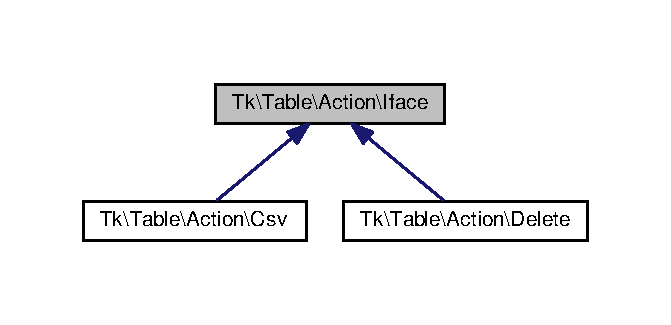
\includegraphics[width=322pt]{classTk_1_1Table_1_1Action_1_1Iface__inherit__graph}
\end{center}
\end{figure}
\subsection*{Public Member Functions}
\begin{DoxyCompactItemize}
\item 
\hyperlink{classTk_1_1Table_1_1Action_1_1Iface_a3da0e0ebded788b5f887988298a8a0af}{\+\_\+\+\_\+construct} (\$name)
\item 
\hyperlink{classTk_1_1Table_1_1Action_1_1Iface_a8aea9f2a29f2d4a256bcd1d3fc89f2ce}{execute} ()
\item 
\hyperlink{classTk_1_1Table_1_1Action_1_1Iface_a900841637cd963f469d8b0a55c691490}{get\+Html} ()
\item 
\hyperlink{classTk_1_1Table_1_1Action_1_1Iface_a6d2c53a8b5d4735c0e454ca63e582b60}{set\+Table} (\$table)
\item 
\hyperlink{classTk_1_1Table_1_1Action_1_1Iface_a8c8c10240620ec4f7caac335f5d388e1}{get\+Table} ()
\item 
\hyperlink{classTk_1_1Table_1_1Action_1_1Iface_ab941a3fabf0613d202a93ac36eaece80}{get\+Name} ()
\item 
\hyperlink{classTk_1_1Table_1_1Action_1_1Iface_a3bff8f4e4bb7348fe5942c38b494e02e}{set\+Name} (\$name)
\item 
\hyperlink{classTk_1_1Table_1_1Action_1_1Iface_ae665bc86c92aef1f43ebb896bf17025d}{get\+Label} ()
\item 
\hyperlink{classTk_1_1Table_1_1Action_1_1Iface_ab7fbf47831804987dda2528da0e8487d}{set\+Label} (\$str)
\item 
\hyperlink{classTk_1_1Table_1_1Action_1_1Iface_af2c7cf179232d0f11b7668992711668f}{add\+Css} (\$class)
\item 
\hyperlink{classTk_1_1Table_1_1Action_1_1Iface_a170ec15504f1ba87c33efa9c622436c6}{remove\+Css} (\$class)
\item 
\hyperlink{classTk_1_1Table_1_1Action_1_1Iface_add82315918344c7f79b8e6760d9f59e1}{get\+Css\+List} ()
\item 
\hyperlink{classTk_1_1Table_1_1Action_1_1Iface_a47f2d195cda44c8ca084243850f0693f}{set\+Css\+List} (\$arr=array())
\end{DoxyCompactItemize}
\subsection*{Protected Attributes}
\begin{DoxyCompactItemize}
\item 
\hypertarget{classTk_1_1Table_1_1Action_1_1Iface_a3b91d6ce23065fe5bbbfe23fcc95cbeb}{{\bfseries \$name} = ''}\label{classTk_1_1Table_1_1Action_1_1Iface_a3b91d6ce23065fe5bbbfe23fcc95cbeb}

\item 
\hypertarget{classTk_1_1Table_1_1Action_1_1Iface_a057704c86e25763fcac5d918d1dbdee7}{{\bfseries \$label} = ''}\label{classTk_1_1Table_1_1Action_1_1Iface_a057704c86e25763fcac5d918d1dbdee7}

\item 
\hypertarget{classTk_1_1Table_1_1Action_1_1Iface_a450b7c941f7d7b932480a65f6cf830f2}{{\bfseries \$css\+List} = array()}\label{classTk_1_1Table_1_1Action_1_1Iface_a450b7c941f7d7b932480a65f6cf830f2}

\item 
\hypertarget{classTk_1_1Table_1_1Action_1_1Iface_a4aee1a7799248870686273189a0b6d0b}{{\bfseries \$table} = null}\label{classTk_1_1Table_1_1Action_1_1Iface_a4aee1a7799248870686273189a0b6d0b}

\end{DoxyCompactItemize}


\subsection{Detailed Description}
The interface for a table Action

\begin{DoxyAuthor}{Author}
Michael Mifsud \href{mailto:info@tropotek.com}{\tt info@tropotek.\+com} \hyperlink{}{Copyright 2015 Michael Mifsud }
\end{DoxyAuthor}


\subsection{Constructor \& Destructor Documentation}
\hypertarget{classTk_1_1Table_1_1Action_1_1Iface_a3da0e0ebded788b5f887988298a8a0af}{\index{Tk\+::\+Table\+::\+Action\+::\+Iface@{Tk\+::\+Table\+::\+Action\+::\+Iface}!\+\_\+\+\_\+construct@{\+\_\+\+\_\+construct}}
\index{\+\_\+\+\_\+construct@{\+\_\+\+\_\+construct}!Tk\+::\+Table\+::\+Action\+::\+Iface@{Tk\+::\+Table\+::\+Action\+::\+Iface}}
\subsubsection[{\+\_\+\+\_\+construct}]{\setlength{\rightskip}{0pt plus 5cm}Tk\textbackslash{}\+Table\textbackslash{}\+Action\textbackslash{}\+Iface\+::\+\_\+\+\_\+construct (
\begin{DoxyParamCaption}
\item[{}]{\$name}
\end{DoxyParamCaption}
)}}\label{classTk_1_1Table_1_1Action_1_1Iface_a3da0e0ebded788b5f887988298a8a0af}
Create


\begin{DoxyParams}[1]{Parameters}
string & {\em \$name} & The action event name \\
\hline
\end{DoxyParams}


\subsection{Member Function Documentation}
\hypertarget{classTk_1_1Table_1_1Action_1_1Iface_af2c7cf179232d0f11b7668992711668f}{\index{Tk\+::\+Table\+::\+Action\+::\+Iface@{Tk\+::\+Table\+::\+Action\+::\+Iface}!add\+Css@{add\+Css}}
\index{add\+Css@{add\+Css}!Tk\+::\+Table\+::\+Action\+::\+Iface@{Tk\+::\+Table\+::\+Action\+::\+Iface}}
\subsubsection[{add\+Css}]{\setlength{\rightskip}{0pt plus 5cm}Tk\textbackslash{}\+Table\textbackslash{}\+Action\textbackslash{}\+Iface\+::add\+Css (
\begin{DoxyParamCaption}
\item[{}]{\$class}
\end{DoxyParamCaption}
)}}\label{classTk_1_1Table_1_1Action_1_1Iface_af2c7cf179232d0f11b7668992711668f}
Add a css class


\begin{DoxyParams}[1]{Parameters}
string & {\em \$class} & \\
\hline
\end{DoxyParams}
\begin{DoxyReturn}{Returns}
\$this 
\end{DoxyReturn}
\hypertarget{classTk_1_1Table_1_1Action_1_1Iface_a8aea9f2a29f2d4a256bcd1d3fc89f2ce}{\index{Tk\+::\+Table\+::\+Action\+::\+Iface@{Tk\+::\+Table\+::\+Action\+::\+Iface}!execute@{execute}}
\index{execute@{execute}!Tk\+::\+Table\+::\+Action\+::\+Iface@{Tk\+::\+Table\+::\+Action\+::\+Iface}}
\subsubsection[{execute}]{\setlength{\rightskip}{0pt plus 5cm}Tk\textbackslash{}\+Table\textbackslash{}\+Action\textbackslash{}\+Iface\+::execute (
\begin{DoxyParamCaption}
{}
\end{DoxyParamCaption}
)\hspace{0.3cm}{\ttfamily [abstract]}}}\label{classTk_1_1Table_1_1Action_1_1Iface_a8aea9f2a29f2d4a256bcd1d3fc89f2ce}
\begin{DoxyReturn}{Returns}
mixed 
\end{DoxyReturn}
\hypertarget{classTk_1_1Table_1_1Action_1_1Iface_add82315918344c7f79b8e6760d9f59e1}{\index{Tk\+::\+Table\+::\+Action\+::\+Iface@{Tk\+::\+Table\+::\+Action\+::\+Iface}!get\+Css\+List@{get\+Css\+List}}
\index{get\+Css\+List@{get\+Css\+List}!Tk\+::\+Table\+::\+Action\+::\+Iface@{Tk\+::\+Table\+::\+Action\+::\+Iface}}
\subsubsection[{get\+Css\+List}]{\setlength{\rightskip}{0pt plus 5cm}Tk\textbackslash{}\+Table\textbackslash{}\+Action\textbackslash{}\+Iface\+::get\+Css\+List (
\begin{DoxyParamCaption}
{}
\end{DoxyParamCaption}
)}}\label{classTk_1_1Table_1_1Action_1_1Iface_add82315918344c7f79b8e6760d9f59e1}
Get the css class list

\begin{DoxyReturn}{Returns}
array 
\end{DoxyReturn}
\hypertarget{classTk_1_1Table_1_1Action_1_1Iface_a900841637cd963f469d8b0a55c691490}{\index{Tk\+::\+Table\+::\+Action\+::\+Iface@{Tk\+::\+Table\+::\+Action\+::\+Iface}!get\+Html@{get\+Html}}
\index{get\+Html@{get\+Html}!Tk\+::\+Table\+::\+Action\+::\+Iface@{Tk\+::\+Table\+::\+Action\+::\+Iface}}
\subsubsection[{get\+Html}]{\setlength{\rightskip}{0pt plus 5cm}Tk\textbackslash{}\+Table\textbackslash{}\+Action\textbackslash{}\+Iface\+::get\+Html (
\begin{DoxyParamCaption}
{}
\end{DoxyParamCaption}
)\hspace{0.3cm}{\ttfamily [abstract]}}}\label{classTk_1_1Table_1_1Action_1_1Iface_a900841637cd963f469d8b0a55c691490}
\begin{DoxyReturn}{Returns}
string$\vert$ 
\end{DoxyReturn}
\hypertarget{classTk_1_1Table_1_1Action_1_1Iface_ae665bc86c92aef1f43ebb896bf17025d}{\index{Tk\+::\+Table\+::\+Action\+::\+Iface@{Tk\+::\+Table\+::\+Action\+::\+Iface}!get\+Label@{get\+Label}}
\index{get\+Label@{get\+Label}!Tk\+::\+Table\+::\+Action\+::\+Iface@{Tk\+::\+Table\+::\+Action\+::\+Iface}}
\subsubsection[{get\+Label}]{\setlength{\rightskip}{0pt plus 5cm}Tk\textbackslash{}\+Table\textbackslash{}\+Action\textbackslash{}\+Iface\+::get\+Label (
\begin{DoxyParamCaption}
{}
\end{DoxyParamCaption}
)}}\label{classTk_1_1Table_1_1Action_1_1Iface_ae665bc86c92aef1f43ebb896bf17025d}
Get the cell label

\begin{DoxyReturn}{Returns}
string 
\end{DoxyReturn}
\hypertarget{classTk_1_1Table_1_1Action_1_1Iface_ab941a3fabf0613d202a93ac36eaece80}{\index{Tk\+::\+Table\+::\+Action\+::\+Iface@{Tk\+::\+Table\+::\+Action\+::\+Iface}!get\+Name@{get\+Name}}
\index{get\+Name@{get\+Name}!Tk\+::\+Table\+::\+Action\+::\+Iface@{Tk\+::\+Table\+::\+Action\+::\+Iface}}
\subsubsection[{get\+Name}]{\setlength{\rightskip}{0pt plus 5cm}Tk\textbackslash{}\+Table\textbackslash{}\+Action\textbackslash{}\+Iface\+::get\+Name (
\begin{DoxyParamCaption}
{}
\end{DoxyParamCaption}
)}}\label{classTk_1_1Table_1_1Action_1_1Iface_ab941a3fabf0613d202a93ac36eaece80}
\begin{DoxyReturn}{Returns}
string 
\end{DoxyReturn}
\hypertarget{classTk_1_1Table_1_1Action_1_1Iface_a8c8c10240620ec4f7caac335f5d388e1}{\index{Tk\+::\+Table\+::\+Action\+::\+Iface@{Tk\+::\+Table\+::\+Action\+::\+Iface}!get\+Table@{get\+Table}}
\index{get\+Table@{get\+Table}!Tk\+::\+Table\+::\+Action\+::\+Iface@{Tk\+::\+Table\+::\+Action\+::\+Iface}}
\subsubsection[{get\+Table}]{\setlength{\rightskip}{0pt plus 5cm}Tk\textbackslash{}\+Table\textbackslash{}\+Action\textbackslash{}\+Iface\+::get\+Table (
\begin{DoxyParamCaption}
{}
\end{DoxyParamCaption}
)}}\label{classTk_1_1Table_1_1Action_1_1Iface_a8c8c10240620ec4f7caac335f5d388e1}
Get the parent table object

\begin{DoxyReturn}{Returns}
\hyperlink{classTk_1_1Table}{Table} 
\end{DoxyReturn}
\hypertarget{classTk_1_1Table_1_1Action_1_1Iface_a170ec15504f1ba87c33efa9c622436c6}{\index{Tk\+::\+Table\+::\+Action\+::\+Iface@{Tk\+::\+Table\+::\+Action\+::\+Iface}!remove\+Css@{remove\+Css}}
\index{remove\+Css@{remove\+Css}!Tk\+::\+Table\+::\+Action\+::\+Iface@{Tk\+::\+Table\+::\+Action\+::\+Iface}}
\subsubsection[{remove\+Css}]{\setlength{\rightskip}{0pt plus 5cm}Tk\textbackslash{}\+Table\textbackslash{}\+Action\textbackslash{}\+Iface\+::remove\+Css (
\begin{DoxyParamCaption}
\item[{}]{\$class}
\end{DoxyParamCaption}
)}}\label{classTk_1_1Table_1_1Action_1_1Iface_a170ec15504f1ba87c33efa9c622436c6}
remove a css class


\begin{DoxyParams}[1]{Parameters}
string & {\em \$class} & \\
\hline
\end{DoxyParams}
\begin{DoxyReturn}{Returns}
\$this 
\end{DoxyReturn}
\hypertarget{classTk_1_1Table_1_1Action_1_1Iface_a47f2d195cda44c8ca084243850f0693f}{\index{Tk\+::\+Table\+::\+Action\+::\+Iface@{Tk\+::\+Table\+::\+Action\+::\+Iface}!set\+Css\+List@{set\+Css\+List}}
\index{set\+Css\+List@{set\+Css\+List}!Tk\+::\+Table\+::\+Action\+::\+Iface@{Tk\+::\+Table\+::\+Action\+::\+Iface}}
\subsubsection[{set\+Css\+List}]{\setlength{\rightskip}{0pt plus 5cm}Tk\textbackslash{}\+Table\textbackslash{}\+Action\textbackslash{}\+Iface\+::set\+Css\+List (
\begin{DoxyParamCaption}
\item[{}]{\$arr = {\ttfamily array()}}
\end{DoxyParamCaption}
)}}\label{classTk_1_1Table_1_1Action_1_1Iface_a47f2d195cda44c8ca084243850f0693f}
Set the css cell class list If no parameter sent the array is cleared.


\begin{DoxyParams}[1]{Parameters}
array & {\em \$arr} & \\
\hline
\end{DoxyParams}
\begin{DoxyReturn}{Returns}
array 
\end{DoxyReturn}
\hypertarget{classTk_1_1Table_1_1Action_1_1Iface_ab7fbf47831804987dda2528da0e8487d}{\index{Tk\+::\+Table\+::\+Action\+::\+Iface@{Tk\+::\+Table\+::\+Action\+::\+Iface}!set\+Label@{set\+Label}}
\index{set\+Label@{set\+Label}!Tk\+::\+Table\+::\+Action\+::\+Iface@{Tk\+::\+Table\+::\+Action\+::\+Iface}}
\subsubsection[{set\+Label}]{\setlength{\rightskip}{0pt plus 5cm}Tk\textbackslash{}\+Table\textbackslash{}\+Action\textbackslash{}\+Iface\+::set\+Label (
\begin{DoxyParamCaption}
\item[{}]{\$str}
\end{DoxyParamCaption}
)}}\label{classTk_1_1Table_1_1Action_1_1Iface_ab7fbf47831804987dda2528da0e8487d}
Set the cell label


\begin{DoxyParams}[1]{Parameters}
string & {\em \$str} & \\
\hline
\end{DoxyParams}
\begin{DoxyReturn}{Returns}
\$this 
\end{DoxyReturn}
\hypertarget{classTk_1_1Table_1_1Action_1_1Iface_a3bff8f4e4bb7348fe5942c38b494e02e}{\index{Tk\+::\+Table\+::\+Action\+::\+Iface@{Tk\+::\+Table\+::\+Action\+::\+Iface}!set\+Name@{set\+Name}}
\index{set\+Name@{set\+Name}!Tk\+::\+Table\+::\+Action\+::\+Iface@{Tk\+::\+Table\+::\+Action\+::\+Iface}}
\subsubsection[{set\+Name}]{\setlength{\rightskip}{0pt plus 5cm}Tk\textbackslash{}\+Table\textbackslash{}\+Action\textbackslash{}\+Iface\+::set\+Name (
\begin{DoxyParamCaption}
\item[{}]{\$name}
\end{DoxyParamCaption}
)}}\label{classTk_1_1Table_1_1Action_1_1Iface_a3bff8f4e4bb7348fe5942c38b494e02e}

\begin{DoxyParams}[1]{Parameters}
string & {\em \$name} & \\
\hline
\end{DoxyParams}
\hypertarget{classTk_1_1Table_1_1Action_1_1Iface_a6d2c53a8b5d4735c0e454ca63e582b60}{\index{Tk\+::\+Table\+::\+Action\+::\+Iface@{Tk\+::\+Table\+::\+Action\+::\+Iface}!set\+Table@{set\+Table}}
\index{set\+Table@{set\+Table}!Tk\+::\+Table\+::\+Action\+::\+Iface@{Tk\+::\+Table\+::\+Action\+::\+Iface}}
\subsubsection[{set\+Table}]{\setlength{\rightskip}{0pt plus 5cm}Tk\textbackslash{}\+Table\textbackslash{}\+Action\textbackslash{}\+Iface\+::set\+Table (
\begin{DoxyParamCaption}
\item[{}]{\$table}
\end{DoxyParamCaption}
)}}\label{classTk_1_1Table_1_1Action_1_1Iface_a6d2c53a8b5d4735c0e454ca63e582b60}
Set the id to be the same as the table. This will be used by the cells for the event key


\begin{DoxyParams}[1]{Parameters}
\hyperlink{classTk_1_1Table}{Table} & {\em \$table} & \\
\hline
\end{DoxyParams}


The documentation for this class was generated from the following file\+:\begin{DoxyCompactItemize}
\item 
vendor/ttek/tk-\/table/\+Tk/\+Table/\+Action/Iface.\+php\end{DoxyCompactItemize}

\hypertarget{classTk_1_1Table_1_1Cell_1_1Iface}{\section{Tk\textbackslash{}Table\textbackslash{}Cell\textbackslash{}Iface Class Reference}
\label{classTk_1_1Table_1_1Cell_1_1Iface}\index{Tk\textbackslash{}\+Table\textbackslash{}\+Cell\textbackslash{}\+Iface@{Tk\textbackslash{}\+Table\textbackslash{}\+Cell\textbackslash{}\+Iface}}
}


Inheritance diagram for Tk\textbackslash{}Table\textbackslash{}Cell\textbackslash{}Iface\+:\nopagebreak
\begin{figure}[H]
\begin{center}
\leavevmode
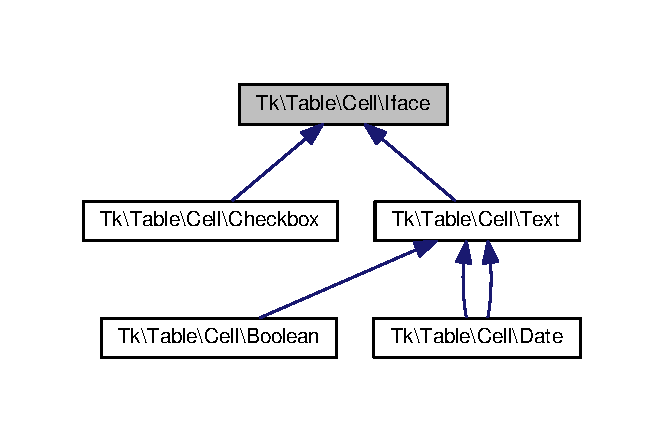
\includegraphics[width=319pt]{classTk_1_1Table_1_1Cell_1_1Iface__inherit__graph}
\end{center}
\end{figure}
\subsection*{Public Member Functions}
\begin{DoxyCompactItemize}
\item 
\hyperlink{classTk_1_1Table_1_1Cell_1_1Iface_a22adb90cf3dbaaf9b57ff81b30d1c5f0}{\+\_\+\+\_\+construct} (\$property, \$label=null)
\item 
\hyperlink{classTk_1_1Table_1_1Cell_1_1Iface_afa44ea3a1a9d0fc44afdc7f08c2a729c}{get\+Cell\+Header} ()
\item 
\hyperlink{classTk_1_1Table_1_1Cell_1_1Iface_ac0eb96286c58f6124f2545ffd23670cf}{get\+Cell\+Html} (\$obj)
\item 
\hyperlink{classTk_1_1Table_1_1Cell_1_1Iface_a17f7cbaa99c95143f835215ef2680967}{get\+Cell\+Csv} (\$obj)
\item 
\hyperlink{classTk_1_1Table_1_1Cell_1_1Iface_a3d600ecdfc436d64f3f924d900c56a55}{get\+Property\+Value} (\$obj, \$property)
\item 
\hyperlink{classTk_1_1Table_1_1Cell_1_1Iface_a9c86a458c2008ca369f1194ed1975e84}{get\+Cell\+Url} (\$obj, \$property= 'id')
\item 
\hyperlink{classTk_1_1Table_1_1Cell_1_1Iface_aad435a709e8b3eab04927afb090cb038}{get\+Order\+Url} ()
\item 
\hyperlink{classTk_1_1Table_1_1Cell_1_1Iface_a651f5d1cbcd908a8ceae0974624eb3e2}{set\+Url} (\$url)
\item 
\hyperlink{classTk_1_1Table_1_1Cell_1_1Iface_a0e0712e54e4d6981c6c38cdd9c19939b}{get\+Url} ()
\item 
\hyperlink{classTk_1_1Table_1_1Cell_1_1Iface_a0aa6b1b55a62947b2e50da5fc40cf459}{set\+Table} (\$table)
\item 
\hyperlink{classTk_1_1Table_1_1Cell_1_1Iface_a0c727f990ef9aeb669d90251c9943cb2}{get\+Table} ()
\item 
\hyperlink{classTk_1_1Table_1_1Cell_1_1Iface_a47be86ee76decc0a80c5dad80decad27}{set\+Show\+Label} (\$b=true)
\item 
\hyperlink{classTk_1_1Table_1_1Cell_1_1Iface_a5210d93e0d33f3faba358edf5be0d1b1}{show\+Label} ()
\item 
\hyperlink{classTk_1_1Table_1_1Cell_1_1Iface_a1447afd0a2d37db622fb3b908012a0a0}{set\+Order\+Property} (\$order\+Property)
\item 
\hyperlink{classTk_1_1Table_1_1Cell_1_1Iface_a868fa3a5f11cb00e5ae8b35bc4c0a51a}{get\+Order\+Property} ()
\item 
\hyperlink{classTk_1_1Table_1_1Cell_1_1Iface_a0cad132c6db216a6326fde14f1c5cec0}{get\+Label} ()
\item 
\hyperlink{classTk_1_1Table_1_1Cell_1_1Iface_a31ffcf0df6c80e3cf45d3724a55f563e}{set\+Label} (\$str)
\item 
\hyperlink{classTk_1_1Table_1_1Cell_1_1Iface_a7a1c6a90b71c5c9ce9d29c0bf12cee14}{get\+Property} ()
\item 
\hyperlink{classTk_1_1Table_1_1Cell_1_1Iface_a975044b186f114ff3ce4c333c8e340b2}{add\+Row\+Css} (\$class)
\item 
\hyperlink{classTk_1_1Table_1_1Cell_1_1Iface_a7dce5bc2a569be6758419acba3ed15ed}{remove\+Row\+Css} (\$class)
\item 
\hyperlink{classTk_1_1Table_1_1Cell_1_1Iface_a32313e3a9e621bfac5e84b5ece724de4}{get\+Row\+Css\+List} ()
\item 
\hyperlink{classTk_1_1Table_1_1Cell_1_1Iface_a071b8a17259b0c662143a6cfd6db84fb}{set\+Row\+Css\+List} (\$arr=array())
\item 
\hyperlink{classTk_1_1Table_1_1Cell_1_1Iface_afd0023e50a4098dce84d1bf479e1a530}{add\+Cell\+Css} (\$class)
\item 
\hyperlink{classTk_1_1Table_1_1Cell_1_1Iface_a24de4dd57000d5a3941b3ad821d77b20}{remove\+Cell\+Css} (\$class)
\item 
\hyperlink{classTk_1_1Table_1_1Cell_1_1Iface_accd53793f78a824dc12953672fc49e7b}{get\+Cell\+Css\+List} ()
\item 
\hyperlink{classTk_1_1Table_1_1Cell_1_1Iface_a5d3867088c8a40a1b371a5f963335e98}{set\+Cell\+Css\+List} (\$arr=array())
\end{DoxyCompactItemize}
\subsection*{Protected Attributes}
\begin{DoxyCompactItemize}
\item 
\hypertarget{classTk_1_1Table_1_1Cell_1_1Iface_a53f677024346cac9651bd24a941cd9c9}{{\bfseries \$label} = ''}\label{classTk_1_1Table_1_1Cell_1_1Iface_a53f677024346cac9651bd24a941cd9c9}

\item 
\hypertarget{classTk_1_1Table_1_1Cell_1_1Iface_aa09321e88bc86b84bb1f7a3a7e9eb6fe}{{\bfseries \$show\+Label} = false}\label{classTk_1_1Table_1_1Cell_1_1Iface_aa09321e88bc86b84bb1f7a3a7e9eb6fe}

\item 
\hypertarget{classTk_1_1Table_1_1Cell_1_1Iface_aedcba96f678bd5a227d40446bdfedc89}{{\bfseries \$property} = ''}\label{classTk_1_1Table_1_1Cell_1_1Iface_aedcba96f678bd5a227d40446bdfedc89}

\item 
\hypertarget{classTk_1_1Table_1_1Cell_1_1Iface_a39c204fc1730b960a536946635fc6f90}{{\bfseries \$cell\+Css\+List} = array()}\label{classTk_1_1Table_1_1Cell_1_1Iface_a39c204fc1730b960a536946635fc6f90}

\item 
\hypertarget{classTk_1_1Table_1_1Cell_1_1Iface_abfec6b5ec6e5eccdc4c58c99015e94fb}{{\bfseries \$row\+Css\+List} = array()}\label{classTk_1_1Table_1_1Cell_1_1Iface_abfec6b5ec6e5eccdc4c58c99015e94fb}

\item 
\hypertarget{classTk_1_1Table_1_1Cell_1_1Iface_a9d428588f1868b9b63e6a73ddb483ae7}{{\bfseries \$order\+Property} = null}\label{classTk_1_1Table_1_1Cell_1_1Iface_a9d428588f1868b9b63e6a73ddb483ae7}

\item 
\hypertarget{classTk_1_1Table_1_1Cell_1_1Iface_a671fa6efd79848b32a4df8e3d65f130b}{{\bfseries \$url} = null}\label{classTk_1_1Table_1_1Cell_1_1Iface_a671fa6efd79848b32a4df8e3d65f130b}

\item 
\hypertarget{classTk_1_1Table_1_1Cell_1_1Iface_a33d0747a090837e9d6cd65ade390cf65}{{\bfseries \$table} = null}\label{classTk_1_1Table_1_1Cell_1_1Iface_a33d0747a090837e9d6cd65ade390cf65}

\end{DoxyCompactItemize}


\subsection{Detailed Description}
The interface for a table Cell

\begin{DoxyAuthor}{Author}
Michael Mifsud \href{mailto:info@tropotek.com}{\tt info@tropotek.\+com} \hyperlink{}{Copyright 2015 Michael Mifsud }
\end{DoxyAuthor}


\subsection{Constructor \& Destructor Documentation}
\hypertarget{classTk_1_1Table_1_1Cell_1_1Iface_a22adb90cf3dbaaf9b57ff81b30d1c5f0}{\index{Tk\+::\+Table\+::\+Cell\+::\+Iface@{Tk\+::\+Table\+::\+Cell\+::\+Iface}!\+\_\+\+\_\+construct@{\+\_\+\+\_\+construct}}
\index{\+\_\+\+\_\+construct@{\+\_\+\+\_\+construct}!Tk\+::\+Table\+::\+Cell\+::\+Iface@{Tk\+::\+Table\+::\+Cell\+::\+Iface}}
\subsubsection[{\+\_\+\+\_\+construct}]{\setlength{\rightskip}{0pt plus 5cm}Tk\textbackslash{}\+Table\textbackslash{}\+Cell\textbackslash{}\+Iface\+::\+\_\+\+\_\+construct (
\begin{DoxyParamCaption}
\item[{}]{\$property, }
\item[{}]{\$label = {\ttfamily null}}
\end{DoxyParamCaption}
)}}\label{classTk_1_1Table_1_1Cell_1_1Iface_a22adb90cf3dbaaf9b57ff81b30d1c5f0}
Create


\begin{DoxyParams}[1]{Parameters}
string & {\em \$property} & \\
\hline
string & {\em \$label} & If null the property name is used E\+G\+: 'prop\+Name' = 'Prop Name' \\
\hline
\end{DoxyParams}


\subsection{Member Function Documentation}
\hypertarget{classTk_1_1Table_1_1Cell_1_1Iface_afd0023e50a4098dce84d1bf479e1a530}{\index{Tk\+::\+Table\+::\+Cell\+::\+Iface@{Tk\+::\+Table\+::\+Cell\+::\+Iface}!add\+Cell\+Css@{add\+Cell\+Css}}
\index{add\+Cell\+Css@{add\+Cell\+Css}!Tk\+::\+Table\+::\+Cell\+::\+Iface@{Tk\+::\+Table\+::\+Cell\+::\+Iface}}
\subsubsection[{add\+Cell\+Css}]{\setlength{\rightskip}{0pt plus 5cm}Tk\textbackslash{}\+Table\textbackslash{}\+Cell\textbackslash{}\+Iface\+::add\+Cell\+Css (
\begin{DoxyParamCaption}
\item[{}]{\$class}
\end{DoxyParamCaption}
)}}\label{classTk_1_1Table_1_1Cell_1_1Iface_afd0023e50a4098dce84d1bf479e1a530}
Add a cell css class


\begin{DoxyParams}[1]{Parameters}
string & {\em \$class} & \\
\hline
\end{DoxyParams}
\begin{DoxyReturn}{Returns}
\$this 
\end{DoxyReturn}
\hypertarget{classTk_1_1Table_1_1Cell_1_1Iface_a975044b186f114ff3ce4c333c8e340b2}{\index{Tk\+::\+Table\+::\+Cell\+::\+Iface@{Tk\+::\+Table\+::\+Cell\+::\+Iface}!add\+Row\+Css@{add\+Row\+Css}}
\index{add\+Row\+Css@{add\+Row\+Css}!Tk\+::\+Table\+::\+Cell\+::\+Iface@{Tk\+::\+Table\+::\+Cell\+::\+Iface}}
\subsubsection[{add\+Row\+Css}]{\setlength{\rightskip}{0pt plus 5cm}Tk\textbackslash{}\+Table\textbackslash{}\+Cell\textbackslash{}\+Iface\+::add\+Row\+Css (
\begin{DoxyParamCaption}
\item[{}]{\$class}
\end{DoxyParamCaption}
)}}\label{classTk_1_1Table_1_1Cell_1_1Iface_a975044b186f114ff3ce4c333c8e340b2}
Add a row css class


\begin{DoxyParams}[1]{Parameters}
string & {\em \$class} & \\
\hline
\end{DoxyParams}
\begin{DoxyReturn}{Returns}
\$this 
\end{DoxyReturn}
\hypertarget{classTk_1_1Table_1_1Cell_1_1Iface_accd53793f78a824dc12953672fc49e7b}{\index{Tk\+::\+Table\+::\+Cell\+::\+Iface@{Tk\+::\+Table\+::\+Cell\+::\+Iface}!get\+Cell\+Css\+List@{get\+Cell\+Css\+List}}
\index{get\+Cell\+Css\+List@{get\+Cell\+Css\+List}!Tk\+::\+Table\+::\+Cell\+::\+Iface@{Tk\+::\+Table\+::\+Cell\+::\+Iface}}
\subsubsection[{get\+Cell\+Css\+List}]{\setlength{\rightskip}{0pt plus 5cm}Tk\textbackslash{}\+Table\textbackslash{}\+Cell\textbackslash{}\+Iface\+::get\+Cell\+Css\+List (
\begin{DoxyParamCaption}
{}
\end{DoxyParamCaption}
)}}\label{classTk_1_1Table_1_1Cell_1_1Iface_accd53793f78a824dc12953672fc49e7b}
Get the css class list

\begin{DoxyReturn}{Returns}
array 
\end{DoxyReturn}
\hypertarget{classTk_1_1Table_1_1Cell_1_1Iface_a17f7cbaa99c95143f835215ef2680967}{\index{Tk\+::\+Table\+::\+Cell\+::\+Iface@{Tk\+::\+Table\+::\+Cell\+::\+Iface}!get\+Cell\+Csv@{get\+Cell\+Csv}}
\index{get\+Cell\+Csv@{get\+Cell\+Csv}!Tk\+::\+Table\+::\+Cell\+::\+Iface@{Tk\+::\+Table\+::\+Cell\+::\+Iface}}
\subsubsection[{get\+Cell\+Csv}]{\setlength{\rightskip}{0pt plus 5cm}Tk\textbackslash{}\+Table\textbackslash{}\+Cell\textbackslash{}\+Iface\+::get\+Cell\+Csv (
\begin{DoxyParamCaption}
\item[{}]{\$obj}
\end{DoxyParamCaption}
)}}\label{classTk_1_1Table_1_1Cell_1_1Iface_a17f7cbaa99c95143f835215ef2680967}

\begin{DoxyParams}[1]{Parameters}
mixed & {\em \$obj} & \\
\hline
\end{DoxyParams}
\begin{DoxyReturn}{Returns}
string 
\end{DoxyReturn}
\hypertarget{classTk_1_1Table_1_1Cell_1_1Iface_afa44ea3a1a9d0fc44afdc7f08c2a729c}{\index{Tk\+::\+Table\+::\+Cell\+::\+Iface@{Tk\+::\+Table\+::\+Cell\+::\+Iface}!get\+Cell\+Header@{get\+Cell\+Header}}
\index{get\+Cell\+Header@{get\+Cell\+Header}!Tk\+::\+Table\+::\+Cell\+::\+Iface@{Tk\+::\+Table\+::\+Cell\+::\+Iface}}
\subsubsection[{get\+Cell\+Header}]{\setlength{\rightskip}{0pt plus 5cm}Tk\textbackslash{}\+Table\textbackslash{}\+Cell\textbackslash{}\+Iface\+::get\+Cell\+Header (
\begin{DoxyParamCaption}
{}
\end{DoxyParamCaption}
)\hspace{0.3cm}{\ttfamily [abstract]}}}\label{classTk_1_1Table_1_1Cell_1_1Iface_afa44ea3a1a9d0fc44afdc7f08c2a729c}
\begin{DoxyReturn}{Returns}
string 
\end{DoxyReturn}
\hypertarget{classTk_1_1Table_1_1Cell_1_1Iface_ac0eb96286c58f6124f2545ffd23670cf}{\index{Tk\+::\+Table\+::\+Cell\+::\+Iface@{Tk\+::\+Table\+::\+Cell\+::\+Iface}!get\+Cell\+Html@{get\+Cell\+Html}}
\index{get\+Cell\+Html@{get\+Cell\+Html}!Tk\+::\+Table\+::\+Cell\+::\+Iface@{Tk\+::\+Table\+::\+Cell\+::\+Iface}}
\subsubsection[{get\+Cell\+Html}]{\setlength{\rightskip}{0pt plus 5cm}Tk\textbackslash{}\+Table\textbackslash{}\+Cell\textbackslash{}\+Iface\+::get\+Cell\+Html (
\begin{DoxyParamCaption}
\item[{}]{\$obj}
\end{DoxyParamCaption}
)\hspace{0.3cm}{\ttfamily [abstract]}}}\label{classTk_1_1Table_1_1Cell_1_1Iface_ac0eb96286c58f6124f2545ffd23670cf}

\begin{DoxyParams}[1]{Parameters}
mixed & {\em \$obj} & \\
\hline
\end{DoxyParams}
\begin{DoxyReturn}{Returns}
string 
\end{DoxyReturn}
\hypertarget{classTk_1_1Table_1_1Cell_1_1Iface_a9c86a458c2008ca369f1194ed1975e84}{\index{Tk\+::\+Table\+::\+Cell\+::\+Iface@{Tk\+::\+Table\+::\+Cell\+::\+Iface}!get\+Cell\+Url@{get\+Cell\+Url}}
\index{get\+Cell\+Url@{get\+Cell\+Url}!Tk\+::\+Table\+::\+Cell\+::\+Iface@{Tk\+::\+Table\+::\+Cell\+::\+Iface}}
\subsubsection[{get\+Cell\+Url}]{\setlength{\rightskip}{0pt plus 5cm}Tk\textbackslash{}\+Table\textbackslash{}\+Cell\textbackslash{}\+Iface\+::get\+Cell\+Url (
\begin{DoxyParamCaption}
\item[{}]{\$obj, }
\item[{}]{\$property = {\ttfamily 'id'}}
\end{DoxyParamCaption}
)}}\label{classTk_1_1Table_1_1Cell_1_1Iface_a9c86a458c2008ca369f1194ed1975e84}
Return the provided U\+R\+L with the G\+E\+T parameter of the object I\+D


\begin{DoxyParams}[1]{Parameters}
mixed & {\em \$obj} & \\
\hline
string & {\em \$property} & \\
\hline
\end{DoxyParams}
\begin{DoxyReturn}{Returns}
Url$\vert$null 
\end{DoxyReturn}
\hypertarget{classTk_1_1Table_1_1Cell_1_1Iface_a0cad132c6db216a6326fde14f1c5cec0}{\index{Tk\+::\+Table\+::\+Cell\+::\+Iface@{Tk\+::\+Table\+::\+Cell\+::\+Iface}!get\+Label@{get\+Label}}
\index{get\+Label@{get\+Label}!Tk\+::\+Table\+::\+Cell\+::\+Iface@{Tk\+::\+Table\+::\+Cell\+::\+Iface}}
\subsubsection[{get\+Label}]{\setlength{\rightskip}{0pt plus 5cm}Tk\textbackslash{}\+Table\textbackslash{}\+Cell\textbackslash{}\+Iface\+::get\+Label (
\begin{DoxyParamCaption}
{}
\end{DoxyParamCaption}
)}}\label{classTk_1_1Table_1_1Cell_1_1Iface_a0cad132c6db216a6326fde14f1c5cec0}
Get the cell label

\begin{DoxyReturn}{Returns}
string 
\end{DoxyReturn}
\hypertarget{classTk_1_1Table_1_1Cell_1_1Iface_a868fa3a5f11cb00e5ae8b35bc4c0a51a}{\index{Tk\+::\+Table\+::\+Cell\+::\+Iface@{Tk\+::\+Table\+::\+Cell\+::\+Iface}!get\+Order\+Property@{get\+Order\+Property}}
\index{get\+Order\+Property@{get\+Order\+Property}!Tk\+::\+Table\+::\+Cell\+::\+Iface@{Tk\+::\+Table\+::\+Cell\+::\+Iface}}
\subsubsection[{get\+Order\+Property}]{\setlength{\rightskip}{0pt plus 5cm}Tk\textbackslash{}\+Table\textbackslash{}\+Cell\textbackslash{}\+Iface\+::get\+Order\+Property (
\begin{DoxyParamCaption}
{}
\end{DoxyParamCaption}
)}}\label{classTk_1_1Table_1_1Cell_1_1Iface_a868fa3a5f11cb00e5ae8b35bc4c0a51a}
Get the order by property name

\begin{DoxyReturn}{Returns}
string 
\end{DoxyReturn}
\hypertarget{classTk_1_1Table_1_1Cell_1_1Iface_aad435a709e8b3eab04927afb090cb038}{\index{Tk\+::\+Table\+::\+Cell\+::\+Iface@{Tk\+::\+Table\+::\+Cell\+::\+Iface}!get\+Order\+Url@{get\+Order\+Url}}
\index{get\+Order\+Url@{get\+Order\+Url}!Tk\+::\+Table\+::\+Cell\+::\+Iface@{Tk\+::\+Table\+::\+Cell\+::\+Iface}}
\subsubsection[{get\+Order\+Url}]{\setlength{\rightskip}{0pt plus 5cm}Tk\textbackslash{}\+Table\textbackslash{}\+Cell\textbackslash{}\+Iface\+::get\+Order\+Url (
\begin{DoxyParamCaption}
{}
\end{DoxyParamCaption}
)}}\label{classTk_1_1Table_1_1Cell_1_1Iface_aad435a709e8b3eab04927afb090cb038}
Create an order by url for this cell.

\begin{DoxyReturn}{Returns}
Url$\vert$null 
\end{DoxyReturn}
\hypertarget{classTk_1_1Table_1_1Cell_1_1Iface_a7a1c6a90b71c5c9ce9d29c0bf12cee14}{\index{Tk\+::\+Table\+::\+Cell\+::\+Iface@{Tk\+::\+Table\+::\+Cell\+::\+Iface}!get\+Property@{get\+Property}}
\index{get\+Property@{get\+Property}!Tk\+::\+Table\+::\+Cell\+::\+Iface@{Tk\+::\+Table\+::\+Cell\+::\+Iface}}
\subsubsection[{get\+Property}]{\setlength{\rightskip}{0pt plus 5cm}Tk\textbackslash{}\+Table\textbackslash{}\+Cell\textbackslash{}\+Iface\+::get\+Property (
\begin{DoxyParamCaption}
{}
\end{DoxyParamCaption}
)}}\label{classTk_1_1Table_1_1Cell_1_1Iface_a7a1c6a90b71c5c9ce9d29c0bf12cee14}
Get the object property name to get data from the object/table

\begin{DoxyReturn}{Returns}
string 
\end{DoxyReturn}
\hypertarget{classTk_1_1Table_1_1Cell_1_1Iface_a3d600ecdfc436d64f3f924d900c56a55}{\index{Tk\+::\+Table\+::\+Cell\+::\+Iface@{Tk\+::\+Table\+::\+Cell\+::\+Iface}!get\+Property\+Value@{get\+Property\+Value}}
\index{get\+Property\+Value@{get\+Property\+Value}!Tk\+::\+Table\+::\+Cell\+::\+Iface@{Tk\+::\+Table\+::\+Cell\+::\+Iface}}
\subsubsection[{get\+Property\+Value}]{\setlength{\rightskip}{0pt plus 5cm}Tk\textbackslash{}\+Table\textbackslash{}\+Cell\textbackslash{}\+Iface\+::get\+Property\+Value (
\begin{DoxyParamCaption}
\item[{}]{\$obj, }
\item[{}]{\$property}
\end{DoxyParamCaption}
)}}\label{classTk_1_1Table_1_1Cell_1_1Iface_a3d600ecdfc436d64f3f924d900c56a55}
Get the property value from the object This should be the clean property data with no H\+T\+M\+L or rendering attached, unless the rendering code is part of the value as it will be called for outputting to other files like X\+M\+L or C\+S\+V.


\begin{DoxyParams}[1]{Parameters}
object & {\em \$obj} & \\
\hline
string & {\em \$property} & \\
\hline
\end{DoxyParams}
\begin{DoxyReturn}{Returns}
mixed 
\end{DoxyReturn}
\hypertarget{classTk_1_1Table_1_1Cell_1_1Iface_a32313e3a9e621bfac5e84b5ece724de4}{\index{Tk\+::\+Table\+::\+Cell\+::\+Iface@{Tk\+::\+Table\+::\+Cell\+::\+Iface}!get\+Row\+Css\+List@{get\+Row\+Css\+List}}
\index{get\+Row\+Css\+List@{get\+Row\+Css\+List}!Tk\+::\+Table\+::\+Cell\+::\+Iface@{Tk\+::\+Table\+::\+Cell\+::\+Iface}}
\subsubsection[{get\+Row\+Css\+List}]{\setlength{\rightskip}{0pt plus 5cm}Tk\textbackslash{}\+Table\textbackslash{}\+Cell\textbackslash{}\+Iface\+::get\+Row\+Css\+List (
\begin{DoxyParamCaption}
{}
\end{DoxyParamCaption}
)}}\label{classTk_1_1Table_1_1Cell_1_1Iface_a32313e3a9e621bfac5e84b5ece724de4}
Get the css row class list

\begin{DoxyReturn}{Returns}
array 
\end{DoxyReturn}
\hypertarget{classTk_1_1Table_1_1Cell_1_1Iface_a0c727f990ef9aeb669d90251c9943cb2}{\index{Tk\+::\+Table\+::\+Cell\+::\+Iface@{Tk\+::\+Table\+::\+Cell\+::\+Iface}!get\+Table@{get\+Table}}
\index{get\+Table@{get\+Table}!Tk\+::\+Table\+::\+Cell\+::\+Iface@{Tk\+::\+Table\+::\+Cell\+::\+Iface}}
\subsubsection[{get\+Table}]{\setlength{\rightskip}{0pt plus 5cm}Tk\textbackslash{}\+Table\textbackslash{}\+Cell\textbackslash{}\+Iface\+::get\+Table (
\begin{DoxyParamCaption}
{}
\end{DoxyParamCaption}
)}}\label{classTk_1_1Table_1_1Cell_1_1Iface_a0c727f990ef9aeb669d90251c9943cb2}
Get the parent table object

\begin{DoxyReturn}{Returns}
\hyperlink{classTk_1_1Table}{Table} 
\end{DoxyReturn}
\hypertarget{classTk_1_1Table_1_1Cell_1_1Iface_a0e0712e54e4d6981c6c38cdd9c19939b}{\index{Tk\+::\+Table\+::\+Cell\+::\+Iface@{Tk\+::\+Table\+::\+Cell\+::\+Iface}!get\+Url@{get\+Url}}
\index{get\+Url@{get\+Url}!Tk\+::\+Table\+::\+Cell\+::\+Iface@{Tk\+::\+Table\+::\+Cell\+::\+Iface}}
\subsubsection[{get\+Url}]{\setlength{\rightskip}{0pt plus 5cm}Tk\textbackslash{}\+Table\textbackslash{}\+Cell\textbackslash{}\+Iface\+::get\+Url (
\begin{DoxyParamCaption}
{}
\end{DoxyParamCaption}
)}}\label{classTk_1_1Table_1_1Cell_1_1Iface_a0e0712e54e4d6981c6c38cdd9c19939b}
Get the default data U\+R\+L

\begin{DoxyReturn}{Returns}
\hyperlink{classTk_1_1Url}{Url} 
\end{DoxyReturn}
\hypertarget{classTk_1_1Table_1_1Cell_1_1Iface_a24de4dd57000d5a3941b3ad821d77b20}{\index{Tk\+::\+Table\+::\+Cell\+::\+Iface@{Tk\+::\+Table\+::\+Cell\+::\+Iface}!remove\+Cell\+Css@{remove\+Cell\+Css}}
\index{remove\+Cell\+Css@{remove\+Cell\+Css}!Tk\+::\+Table\+::\+Cell\+::\+Iface@{Tk\+::\+Table\+::\+Cell\+::\+Iface}}
\subsubsection[{remove\+Cell\+Css}]{\setlength{\rightskip}{0pt plus 5cm}Tk\textbackslash{}\+Table\textbackslash{}\+Cell\textbackslash{}\+Iface\+::remove\+Cell\+Css (
\begin{DoxyParamCaption}
\item[{}]{\$class}
\end{DoxyParamCaption}
)}}\label{classTk_1_1Table_1_1Cell_1_1Iface_a24de4dd57000d5a3941b3ad821d77b20}
remove a css class


\begin{DoxyParams}[1]{Parameters}
string & {\em \$class} & \\
\hline
\end{DoxyParams}
\begin{DoxyReturn}{Returns}
\$this 
\end{DoxyReturn}
\hypertarget{classTk_1_1Table_1_1Cell_1_1Iface_a7dce5bc2a569be6758419acba3ed15ed}{\index{Tk\+::\+Table\+::\+Cell\+::\+Iface@{Tk\+::\+Table\+::\+Cell\+::\+Iface}!remove\+Row\+Css@{remove\+Row\+Css}}
\index{remove\+Row\+Css@{remove\+Row\+Css}!Tk\+::\+Table\+::\+Cell\+::\+Iface@{Tk\+::\+Table\+::\+Cell\+::\+Iface}}
\subsubsection[{remove\+Row\+Css}]{\setlength{\rightskip}{0pt plus 5cm}Tk\textbackslash{}\+Table\textbackslash{}\+Cell\textbackslash{}\+Iface\+::remove\+Row\+Css (
\begin{DoxyParamCaption}
\item[{}]{\$class}
\end{DoxyParamCaption}
)}}\label{classTk_1_1Table_1_1Cell_1_1Iface_a7dce5bc2a569be6758419acba3ed15ed}
remove a row css class


\begin{DoxyParams}[1]{Parameters}
string & {\em \$class} & \\
\hline
\end{DoxyParams}
\begin{DoxyReturn}{Returns}
\$this 
\end{DoxyReturn}
\hypertarget{classTk_1_1Table_1_1Cell_1_1Iface_a5d3867088c8a40a1b371a5f963335e98}{\index{Tk\+::\+Table\+::\+Cell\+::\+Iface@{Tk\+::\+Table\+::\+Cell\+::\+Iface}!set\+Cell\+Css\+List@{set\+Cell\+Css\+List}}
\index{set\+Cell\+Css\+List@{set\+Cell\+Css\+List}!Tk\+::\+Table\+::\+Cell\+::\+Iface@{Tk\+::\+Table\+::\+Cell\+::\+Iface}}
\subsubsection[{set\+Cell\+Css\+List}]{\setlength{\rightskip}{0pt plus 5cm}Tk\textbackslash{}\+Table\textbackslash{}\+Cell\textbackslash{}\+Iface\+::set\+Cell\+Css\+List (
\begin{DoxyParamCaption}
\item[{}]{\$arr = {\ttfamily array()}}
\end{DoxyParamCaption}
)}}\label{classTk_1_1Table_1_1Cell_1_1Iface_a5d3867088c8a40a1b371a5f963335e98}
Set the css cell class list If no parameter sent the array is cleared.


\begin{DoxyParams}[1]{Parameters}
array & {\em \$arr} & \\
\hline
\end{DoxyParams}
\begin{DoxyReturn}{Returns}
array 
\end{DoxyReturn}
\hypertarget{classTk_1_1Table_1_1Cell_1_1Iface_a31ffcf0df6c80e3cf45d3724a55f563e}{\index{Tk\+::\+Table\+::\+Cell\+::\+Iface@{Tk\+::\+Table\+::\+Cell\+::\+Iface}!set\+Label@{set\+Label}}
\index{set\+Label@{set\+Label}!Tk\+::\+Table\+::\+Cell\+::\+Iface@{Tk\+::\+Table\+::\+Cell\+::\+Iface}}
\subsubsection[{set\+Label}]{\setlength{\rightskip}{0pt plus 5cm}Tk\textbackslash{}\+Table\textbackslash{}\+Cell\textbackslash{}\+Iface\+::set\+Label (
\begin{DoxyParamCaption}
\item[{}]{\$str}
\end{DoxyParamCaption}
)}}\label{classTk_1_1Table_1_1Cell_1_1Iface_a31ffcf0df6c80e3cf45d3724a55f563e}
Set the cell label


\begin{DoxyParams}[1]{Parameters}
string & {\em \$str} & \\
\hline
\end{DoxyParams}
\begin{DoxyReturn}{Returns}
\$this 
\end{DoxyReturn}
\hypertarget{classTk_1_1Table_1_1Cell_1_1Iface_a1447afd0a2d37db622fb3b908012a0a0}{\index{Tk\+::\+Table\+::\+Cell\+::\+Iface@{Tk\+::\+Table\+::\+Cell\+::\+Iface}!set\+Order\+Property@{set\+Order\+Property}}
\index{set\+Order\+Property@{set\+Order\+Property}!Tk\+::\+Table\+::\+Cell\+::\+Iface@{Tk\+::\+Table\+::\+Cell\+::\+Iface}}
\subsubsection[{set\+Order\+Property}]{\setlength{\rightskip}{0pt plus 5cm}Tk\textbackslash{}\+Table\textbackslash{}\+Cell\textbackslash{}\+Iface\+::set\+Order\+Property (
\begin{DoxyParamCaption}
\item[{}]{\$order\+Property}
\end{DoxyParamCaption}
)}}\label{classTk_1_1Table_1_1Cell_1_1Iface_a1447afd0a2d37db622fb3b908012a0a0}
Set the property that the order header uses by default this is the same as property


\begin{DoxyParams}[1]{Parameters}
string & {\em \$order\+Property} & \\
\hline
\end{DoxyParams}
\begin{DoxyReturn}{Returns}
\$this 
\end{DoxyReturn}
\hypertarget{classTk_1_1Table_1_1Cell_1_1Iface_a071b8a17259b0c662143a6cfd6db84fb}{\index{Tk\+::\+Table\+::\+Cell\+::\+Iface@{Tk\+::\+Table\+::\+Cell\+::\+Iface}!set\+Row\+Css\+List@{set\+Row\+Css\+List}}
\index{set\+Row\+Css\+List@{set\+Row\+Css\+List}!Tk\+::\+Table\+::\+Cell\+::\+Iface@{Tk\+::\+Table\+::\+Cell\+::\+Iface}}
\subsubsection[{set\+Row\+Css\+List}]{\setlength{\rightskip}{0pt plus 5cm}Tk\textbackslash{}\+Table\textbackslash{}\+Cell\textbackslash{}\+Iface\+::set\+Row\+Css\+List (
\begin{DoxyParamCaption}
\item[{}]{\$arr = {\ttfamily array()}}
\end{DoxyParamCaption}
)}}\label{classTk_1_1Table_1_1Cell_1_1Iface_a071b8a17259b0c662143a6cfd6db84fb}
Set the css row class list If no parameter sent the array is cleared.


\begin{DoxyParams}[1]{Parameters}
array & {\em \$arr} & \\
\hline
\end{DoxyParams}
\begin{DoxyReturn}{Returns}
array 
\end{DoxyReturn}
\hypertarget{classTk_1_1Table_1_1Cell_1_1Iface_a47be86ee76decc0a80c5dad80decad27}{\index{Tk\+::\+Table\+::\+Cell\+::\+Iface@{Tk\+::\+Table\+::\+Cell\+::\+Iface}!set\+Show\+Label@{set\+Show\+Label}}
\index{set\+Show\+Label@{set\+Show\+Label}!Tk\+::\+Table\+::\+Cell\+::\+Iface@{Tk\+::\+Table\+::\+Cell\+::\+Iface}}
\subsubsection[{set\+Show\+Label}]{\setlength{\rightskip}{0pt plus 5cm}Tk\textbackslash{}\+Table\textbackslash{}\+Cell\textbackslash{}\+Iface\+::set\+Show\+Label (
\begin{DoxyParamCaption}
\item[{}]{\$b = {\ttfamily true}}
\end{DoxyParamCaption}
)}}\label{classTk_1_1Table_1_1Cell_1_1Iface_a47be86ee76decc0a80c5dad80decad27}
If set the label will be rendered This depends on the table renderer being used.


\begin{DoxyParams}[1]{Parameters}
bool & {\em \$b} & \\
\hline
\end{DoxyParams}
\begin{DoxyReturn}{Returns}
\$this 
\end{DoxyReturn}
\hypertarget{classTk_1_1Table_1_1Cell_1_1Iface_a0aa6b1b55a62947b2e50da5fc40cf459}{\index{Tk\+::\+Table\+::\+Cell\+::\+Iface@{Tk\+::\+Table\+::\+Cell\+::\+Iface}!set\+Table@{set\+Table}}
\index{set\+Table@{set\+Table}!Tk\+::\+Table\+::\+Cell\+::\+Iface@{Tk\+::\+Table\+::\+Cell\+::\+Iface}}
\subsubsection[{set\+Table}]{\setlength{\rightskip}{0pt plus 5cm}Tk\textbackslash{}\+Table\textbackslash{}\+Cell\textbackslash{}\+Iface\+::set\+Table (
\begin{DoxyParamCaption}
\item[{}]{\$table}
\end{DoxyParamCaption}
)}}\label{classTk_1_1Table_1_1Cell_1_1Iface_a0aa6b1b55a62947b2e50da5fc40cf459}
Set the id to be the same as the table. This will be used by the cells for the event key


\begin{DoxyParams}[1]{Parameters}
\hyperlink{classTk_1_1Table}{Table} & {\em \$table} & \\
\hline
\end{DoxyParams}
\hypertarget{classTk_1_1Table_1_1Cell_1_1Iface_a651f5d1cbcd908a8ceae0974624eb3e2}{\index{Tk\+::\+Table\+::\+Cell\+::\+Iface@{Tk\+::\+Table\+::\+Cell\+::\+Iface}!set\+Url@{set\+Url}}
\index{set\+Url@{set\+Url}!Tk\+::\+Table\+::\+Cell\+::\+Iface@{Tk\+::\+Table\+::\+Cell\+::\+Iface}}
\subsubsection[{set\+Url}]{\setlength{\rightskip}{0pt plus 5cm}Tk\textbackslash{}\+Table\textbackslash{}\+Cell\textbackslash{}\+Iface\+::set\+Url (
\begin{DoxyParamCaption}
\item[{}]{\$url}
\end{DoxyParamCaption}
)}}\label{classTk_1_1Table_1_1Cell_1_1Iface_a651f5d1cbcd908a8ceae0974624eb3e2}
Set the default cell data url


\begin{DoxyParams}[1]{Parameters}
\hyperlink{classTk_1_1Url}{Url} & {\em \$url} & \\
\hline
\end{DoxyParams}
\begin{DoxyReturn}{Returns}
\$this 
\end{DoxyReturn}
\hypertarget{classTk_1_1Table_1_1Cell_1_1Iface_a5210d93e0d33f3faba358edf5be0d1b1}{\index{Tk\+::\+Table\+::\+Cell\+::\+Iface@{Tk\+::\+Table\+::\+Cell\+::\+Iface}!show\+Label@{show\+Label}}
\index{show\+Label@{show\+Label}!Tk\+::\+Table\+::\+Cell\+::\+Iface@{Tk\+::\+Table\+::\+Cell\+::\+Iface}}
\subsubsection[{show\+Label}]{\setlength{\rightskip}{0pt plus 5cm}Tk\textbackslash{}\+Table\textbackslash{}\+Cell\textbackslash{}\+Iface\+::show\+Label (
\begin{DoxyParamCaption}
{}
\end{DoxyParamCaption}
)}}\label{classTk_1_1Table_1_1Cell_1_1Iface_a5210d93e0d33f3faba358edf5be0d1b1}
get\+Show\+Label

\begin{DoxyReturn}{Returns}
bool 
\end{DoxyReturn}


The documentation for this class was generated from the following file\+:\begin{DoxyCompactItemize}
\item 
vendor/ttek/tk-\/table/\+Tk/\+Table/\+Cell/Iface.\+php\end{DoxyCompactItemize}

\hypertarget{classTk_1_1Table_1_1Renderer_1_1Dom_1_1Ui_1_1Iface}{\section{Tk\textbackslash{}Table\textbackslash{}Renderer\textbackslash{}Dom\textbackslash{}Ui\textbackslash{}Iface Class Reference}
\label{classTk_1_1Table_1_1Renderer_1_1Dom_1_1Ui_1_1Iface}\index{Tk\textbackslash{}\+Table\textbackslash{}\+Renderer\textbackslash{}\+Dom\textbackslash{}\+Ui\textbackslash{}\+Iface@{Tk\textbackslash{}\+Table\textbackslash{}\+Renderer\textbackslash{}\+Dom\textbackslash{}\+Ui\textbackslash{}\+Iface}}
}


Inheritance diagram for Tk\textbackslash{}Table\textbackslash{}Renderer\textbackslash{}Dom\textbackslash{}Ui\textbackslash{}Iface\+:\nopagebreak
\begin{figure}[H]
\begin{center}
\leavevmode
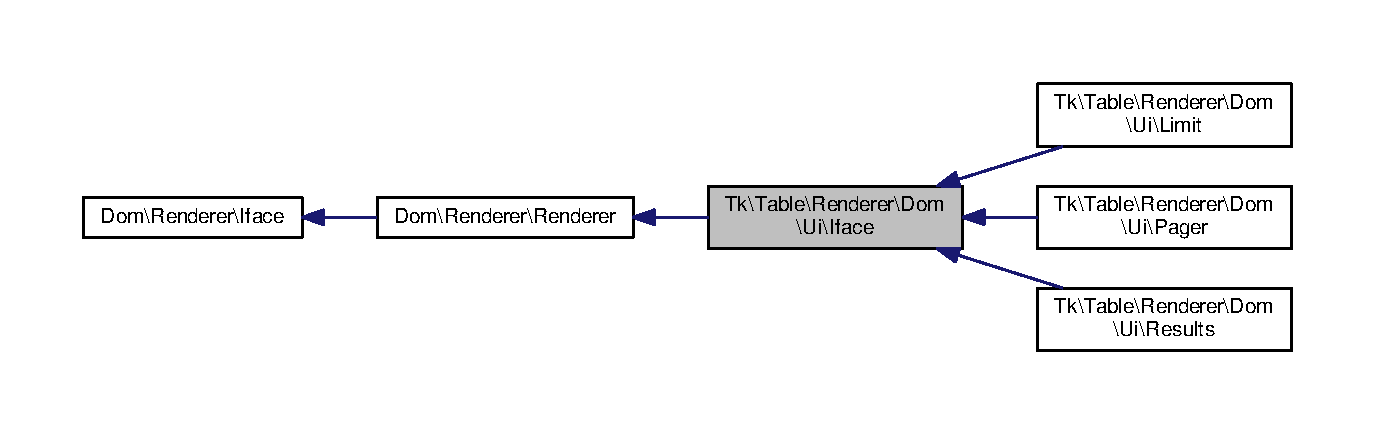
\includegraphics[width=350pt]{classTk_1_1Table_1_1Renderer_1_1Dom_1_1Ui_1_1Iface__inherit__graph}
\end{center}
\end{figure}
\subsection*{Public Member Functions}
\begin{DoxyCompactItemize}
\item 
\hyperlink{classTk_1_1Table_1_1Renderer_1_1Dom_1_1Ui_1_1Iface_a1c08dbab4332e72f3f24d64c27560a45}{add\+Css\+Class} (\$css)
\end{DoxyCompactItemize}
\subsection*{Public Attributes}
\begin{DoxyCompactItemize}
\item 
\hypertarget{classTk_1_1Table_1_1Renderer_1_1Dom_1_1Ui_1_1Iface_abbff1c3d744a2e7fa950194e2db86577}{const {\bfseries P\+A\+R\+A\+M\+\_\+\+L\+I\+M\+I\+T} = 'limit'}\label{classTk_1_1Table_1_1Renderer_1_1Dom_1_1Ui_1_1Iface_abbff1c3d744a2e7fa950194e2db86577}

\item 
\hypertarget{classTk_1_1Table_1_1Renderer_1_1Dom_1_1Ui_1_1Iface_a62e55af6b8dcc022f55c7ec2fff1e5c3}{const {\bfseries P\+A\+R\+A\+M\+\_\+\+O\+F\+F\+S\+E\+T} = 'offset'}\label{classTk_1_1Table_1_1Renderer_1_1Dom_1_1Ui_1_1Iface_a62e55af6b8dcc022f55c7ec2fff1e5c3}

\item 
\hypertarget{classTk_1_1Table_1_1Renderer_1_1Dom_1_1Ui_1_1Iface_ab612051e625a9b7a956301b4ffcf7b10}{const {\bfseries P\+A\+R\+A\+M\+\_\+\+T\+O\+T\+A\+L} = 'total'}\label{classTk_1_1Table_1_1Renderer_1_1Dom_1_1Ui_1_1Iface_ab612051e625a9b7a956301b4ffcf7b10}

\item 
\hypertarget{classTk_1_1Table_1_1Renderer_1_1Dom_1_1Ui_1_1Iface_a321e84b5737c6fbc51ebe07e22144b66}{const {\bfseries C\+S\+S\+\_\+\+S\+E\+L\+E\+C\+T\+E\+D} = 'active'}\label{classTk_1_1Table_1_1Renderer_1_1Dom_1_1Ui_1_1Iface_a321e84b5737c6fbc51ebe07e22144b66}

\item 
\hypertarget{classTk_1_1Table_1_1Renderer_1_1Dom_1_1Ui_1_1Iface_af4a693de83af7c632bd14077033f7fe8}{const {\bfseries C\+S\+S\+\_\+\+D\+I\+S\+A\+B\+L\+E\+D} = 'disabled'}\label{classTk_1_1Table_1_1Renderer_1_1Dom_1_1Ui_1_1Iface_af4a693de83af7c632bd14077033f7fe8}

\end{DoxyCompactItemize}
\subsection*{Protected Attributes}
\begin{DoxyCompactItemize}
\item 
\hypertarget{classTk_1_1Table_1_1Renderer_1_1Dom_1_1Ui_1_1Iface_ad87ae63ddb57b025fcc68b34315ab7df}{{\bfseries \$css\+List} = array()}\label{classTk_1_1Table_1_1Renderer_1_1Dom_1_1Ui_1_1Iface_ad87ae63ddb57b025fcc68b34315ab7df}

\end{DoxyCompactItemize}


\subsection{Detailed Description}
Class \hyperlink{classTk_1_1Table_1_1Renderer_1_1Dom_1_1Ui_1_1Iface}{Iface}

\begin{DoxyAuthor}{Author}
Michael Mifsud \href{mailto:info@tropotek.com}{\tt info@tropotek.\+com} \hyperlink{}{Copyright 2015 Michael Mifsud }
\end{DoxyAuthor}


\subsection{Member Function Documentation}
\hypertarget{classTk_1_1Table_1_1Renderer_1_1Dom_1_1Ui_1_1Iface_a1c08dbab4332e72f3f24d64c27560a45}{\index{Tk\+::\+Table\+::\+Renderer\+::\+Dom\+::\+Ui\+::\+Iface@{Tk\+::\+Table\+::\+Renderer\+::\+Dom\+::\+Ui\+::\+Iface}!add\+Css\+Class@{add\+Css\+Class}}
\index{add\+Css\+Class@{add\+Css\+Class}!Tk\+::\+Table\+::\+Renderer\+::\+Dom\+::\+Ui\+::\+Iface@{Tk\+::\+Table\+::\+Renderer\+::\+Dom\+::\+Ui\+::\+Iface}}
\subsubsection[{add\+Css\+Class}]{\setlength{\rightskip}{0pt plus 5cm}Tk\textbackslash{}\+Table\textbackslash{}\+Renderer\textbackslash{}\+Dom\textbackslash{}\+Ui\textbackslash{}\+Iface\+::add\+Css\+Class (
\begin{DoxyParamCaption}
\item[{}]{\$css}
\end{DoxyParamCaption}
)}}\label{classTk_1_1Table_1_1Renderer_1_1Dom_1_1Ui_1_1Iface_a1c08dbab4332e72f3f24d64c27560a45}
Set the css classes to append to the root node


\begin{DoxyParams}{Parameters}
{\em \$css} & \\
\hline
\end{DoxyParams}


The documentation for this class was generated from the following file\+:\begin{DoxyCompactItemize}
\item 
vendor/ttek/tk-\/table/\+Tk/\+Table/\+Renderer/\+Dom/\+Ui/Iface.\+php\end{DoxyCompactItemize}

\hypertarget{classTk_1_1Table_1_1Renderer_1_1Iface}{\section{Tk\textbackslash{}Table\textbackslash{}Renderer\textbackslash{}Iface Class Reference}
\label{classTk_1_1Table_1_1Renderer_1_1Iface}\index{Tk\textbackslash{}\+Table\textbackslash{}\+Renderer\textbackslash{}\+Iface@{Tk\textbackslash{}\+Table\textbackslash{}\+Renderer\textbackslash{}\+Iface}}
}


Inheritance diagram for Tk\textbackslash{}Table\textbackslash{}Renderer\textbackslash{}Iface\+:\nopagebreak
\begin{figure}[H]
\begin{center}
\leavevmode
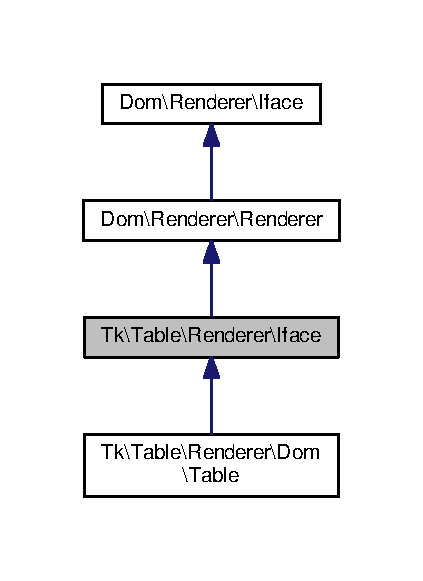
\includegraphics[width=203pt]{classTk_1_1Table_1_1Renderer_1_1Iface__inherit__graph}
\end{center}
\end{figure}
\subsection*{Public Member Functions}
\begin{DoxyCompactItemize}
\item 
\hyperlink{classTk_1_1Table_1_1Renderer_1_1Iface_a0dc0aee58d8b85c8ef927bd872d86cf7}{\+\_\+\+\_\+construct} (\$table=null)
\item 
\hyperlink{classTk_1_1Table_1_1Renderer_1_1Iface_a160e91cba1b6e1fbde406a99b9dbaa99}{set\+Table} (\$table)
\item 
\hyperlink{classTk_1_1Table_1_1Renderer_1_1Iface_a18950454d6c078fa30dbdeb166304a78}{get\+Table} ()
\item 
\hyperlink{classTk_1_1Table_1_1Renderer_1_1Iface_a7a67228562c01a78aab1f4f53dae6e82}{append\+Foot\+Renderer} (\$renderer)
\item 
\hyperlink{classTk_1_1Table_1_1Renderer_1_1Iface_a72d642c266fadc5610e9fb42ed8480c5}{get\+Footer\+Render\+List} ()
\item 
\hyperlink{classTk_1_1Table_1_1Renderer_1_1Iface_a2a342af495394bc1b15da8e8a4b9f8ec}{set\+Footer\+Render\+List} (\$foot\+Render\+List)
\item 
\hyperlink{classTk_1_1Table_1_1Renderer_1_1Iface_a5afb7e3ac6b4368bf22a341bb1541b42}{get\+Row\+Id} ()
\end{DoxyCompactItemize}
\subsection*{Protected Member Functions}
\begin{DoxyCompactItemize}
\item 
\hyperlink{classTk_1_1Table_1_1Renderer_1_1Iface_af867242ecfb4b072b1477e9d267842ce}{init\+Filter\+Form} ()
\item 
\hyperlink{classTk_1_1Table_1_1Renderer_1_1Iface_a804b5db07a8704fbde1a354c0f41cd19}{show\+Header} ()
\item 
\hyperlink{classTk_1_1Table_1_1Renderer_1_1Iface_a38112665a39f4632e874da31c6406c3a}{show\+Body} ()
\item 
\hyperlink{classTk_1_1Table_1_1Renderer_1_1Iface_ae7848d09be2e5531784e607a9e0044bc}{show\+Row} (\$obj)
\item 
\hyperlink{classTk_1_1Table_1_1Renderer_1_1Iface_a3fd613e8182bd0cbc6f6deb6f6de9055}{show\+Cell} (\hyperlink{classTk_1_1Table_1_1Cell_1_1Iface}{Cell\textbackslash{}\+Iface} \$cell, \$obj)
\item 
\hyperlink{classTk_1_1Table_1_1Renderer_1_1Iface_a91dfeafc861134a1b4f8f40d637b3a87}{show\+Footer} ()
\end{DoxyCompactItemize}
\subsection*{Protected Attributes}
\begin{DoxyCompactItemize}
\item 
\hypertarget{classTk_1_1Table_1_1Renderer_1_1Iface_a9b9673e6458d2ce575f3522c9e942f2f}{{\bfseries \$table} = null}\label{classTk_1_1Table_1_1Renderer_1_1Iface_a9b9673e6458d2ce575f3522c9e942f2f}

\item 
\hypertarget{classTk_1_1Table_1_1Renderer_1_1Iface_a2ac2a8f817b4849b0b5d787cb8a83f0f}{{\bfseries \$foot\+Render\+List} = array()}\label{classTk_1_1Table_1_1Renderer_1_1Iface_a2ac2a8f817b4849b0b5d787cb8a83f0f}

\item 
\hypertarget{classTk_1_1Table_1_1Renderer_1_1Iface_a1a8c7c7b124e173cb99f1b2ce430d933}{{\bfseries \$row\+Id} = 0}\label{classTk_1_1Table_1_1Renderer_1_1Iface_a1a8c7c7b124e173cb99f1b2ce430d933}

\end{DoxyCompactItemize}


\subsection{Detailed Description}
Class \hyperlink{classTk_1_1Table_1_1Renderer_1_1Iface}{Iface}

\begin{DoxyAuthor}{Author}
Michael Mifsud \href{mailto:info@tropotek.com}{\tt info@tropotek.\+com} \hyperlink{}{Copyright 2015 Michael Mifsud }
\end{DoxyAuthor}


\subsection{Constructor \& Destructor Documentation}
\hypertarget{classTk_1_1Table_1_1Renderer_1_1Iface_a0dc0aee58d8b85c8ef927bd872d86cf7}{\index{Tk\+::\+Table\+::\+Renderer\+::\+Iface@{Tk\+::\+Table\+::\+Renderer\+::\+Iface}!\+\_\+\+\_\+construct@{\+\_\+\+\_\+construct}}
\index{\+\_\+\+\_\+construct@{\+\_\+\+\_\+construct}!Tk\+::\+Table\+::\+Renderer\+::\+Iface@{Tk\+::\+Table\+::\+Renderer\+::\+Iface}}
\subsubsection[{\+\_\+\+\_\+construct}]{\setlength{\rightskip}{0pt plus 5cm}Tk\textbackslash{}\+Table\textbackslash{}\+Renderer\textbackslash{}\+Iface\+::\+\_\+\+\_\+construct (
\begin{DoxyParamCaption}
\item[{}]{\$table = {\ttfamily null}}
\end{DoxyParamCaption}
)}}\label{classTk_1_1Table_1_1Renderer_1_1Iface_a0dc0aee58d8b85c8ef927bd872d86cf7}
construct


\begin{DoxyParams}[1]{Parameters}
\hyperlink{classTk_1_1Table}{Table} & {\em \$table} & \\
\hline
\end{DoxyParams}


\subsection{Member Function Documentation}
\hypertarget{classTk_1_1Table_1_1Renderer_1_1Iface_a7a67228562c01a78aab1f4f53dae6e82}{\index{Tk\+::\+Table\+::\+Renderer\+::\+Iface@{Tk\+::\+Table\+::\+Renderer\+::\+Iface}!append\+Foot\+Renderer@{append\+Foot\+Renderer}}
\index{append\+Foot\+Renderer@{append\+Foot\+Renderer}!Tk\+::\+Table\+::\+Renderer\+::\+Iface@{Tk\+::\+Table\+::\+Renderer\+::\+Iface}}
\subsubsection[{append\+Foot\+Renderer}]{\setlength{\rightskip}{0pt plus 5cm}Tk\textbackslash{}\+Table\textbackslash{}\+Renderer\textbackslash{}\+Iface\+::append\+Foot\+Renderer (
\begin{DoxyParamCaption}
\item[{}]{\$renderer}
\end{DoxyParamCaption}
)}}\label{classTk_1_1Table_1_1Renderer_1_1Iface_a7a67228562c01a78aab1f4f53dae6e82}
Append a renderer to the footer renderer list


\begin{DoxyParams}[1]{Parameters}
mixed & {\em \$renderer} & \\
\hline
\end{DoxyParams}
\hypertarget{classTk_1_1Table_1_1Renderer_1_1Iface_a72d642c266fadc5610e9fb42ed8480c5}{\index{Tk\+::\+Table\+::\+Renderer\+::\+Iface@{Tk\+::\+Table\+::\+Renderer\+::\+Iface}!get\+Footer\+Render\+List@{get\+Footer\+Render\+List}}
\index{get\+Footer\+Render\+List@{get\+Footer\+Render\+List}!Tk\+::\+Table\+::\+Renderer\+::\+Iface@{Tk\+::\+Table\+::\+Renderer\+::\+Iface}}
\subsubsection[{get\+Footer\+Render\+List}]{\setlength{\rightskip}{0pt plus 5cm}Tk\textbackslash{}\+Table\textbackslash{}\+Renderer\textbackslash{}\+Iface\+::get\+Footer\+Render\+List (
\begin{DoxyParamCaption}
{}
\end{DoxyParamCaption}
)}}\label{classTk_1_1Table_1_1Renderer_1_1Iface_a72d642c266fadc5610e9fb42ed8480c5}
\begin{DoxyReturn}{Returns}
array 
\end{DoxyReturn}
\hypertarget{classTk_1_1Table_1_1Renderer_1_1Iface_a5afb7e3ac6b4368bf22a341bb1541b42}{\index{Tk\+::\+Table\+::\+Renderer\+::\+Iface@{Tk\+::\+Table\+::\+Renderer\+::\+Iface}!get\+Row\+Id@{get\+Row\+Id}}
\index{get\+Row\+Id@{get\+Row\+Id}!Tk\+::\+Table\+::\+Renderer\+::\+Iface@{Tk\+::\+Table\+::\+Renderer\+::\+Iface}}
\subsubsection[{get\+Row\+Id}]{\setlength{\rightskip}{0pt plus 5cm}Tk\textbackslash{}\+Table\textbackslash{}\+Renderer\textbackslash{}\+Iface\+::get\+Row\+Id (
\begin{DoxyParamCaption}
{}
\end{DoxyParamCaption}
)}}\label{classTk_1_1Table_1_1Renderer_1_1Iface_a5afb7e3ac6b4368bf22a341bb1541b42}
Return the current row being rendered. t\+This value should take any offest into account.

\begin{DoxyReturn}{Returns}
int 
\end{DoxyReturn}
\hypertarget{classTk_1_1Table_1_1Renderer_1_1Iface_a18950454d6c078fa30dbdeb166304a78}{\index{Tk\+::\+Table\+::\+Renderer\+::\+Iface@{Tk\+::\+Table\+::\+Renderer\+::\+Iface}!get\+Table@{get\+Table}}
\index{get\+Table@{get\+Table}!Tk\+::\+Table\+::\+Renderer\+::\+Iface@{Tk\+::\+Table\+::\+Renderer\+::\+Iface}}
\subsubsection[{get\+Table}]{\setlength{\rightskip}{0pt plus 5cm}Tk\textbackslash{}\+Table\textbackslash{}\+Renderer\textbackslash{}\+Iface\+::get\+Table (
\begin{DoxyParamCaption}
{}
\end{DoxyParamCaption}
)}}\label{classTk_1_1Table_1_1Renderer_1_1Iface_a18950454d6c078fa30dbdeb166304a78}
Get the table

\begin{DoxyReturn}{Returns}
\hyperlink{classTk_1_1Table}{Table} 
\end{DoxyReturn}
\hypertarget{classTk_1_1Table_1_1Renderer_1_1Iface_af867242ecfb4b072b1477e9d267842ce}{\index{Tk\+::\+Table\+::\+Renderer\+::\+Iface@{Tk\+::\+Table\+::\+Renderer\+::\+Iface}!init\+Filter\+Form@{init\+Filter\+Form}}
\index{init\+Filter\+Form@{init\+Filter\+Form}!Tk\+::\+Table\+::\+Renderer\+::\+Iface@{Tk\+::\+Table\+::\+Renderer\+::\+Iface}}
\subsubsection[{init\+Filter\+Form}]{\setlength{\rightskip}{0pt plus 5cm}Tk\textbackslash{}\+Table\textbackslash{}\+Renderer\textbackslash{}\+Iface\+::init\+Filter\+Form (
\begin{DoxyParamCaption}
{}
\end{DoxyParamCaption}
)\hspace{0.3cm}{\ttfamily [abstract]}, {\ttfamily [protected]}}}\label{classTk_1_1Table_1_1Renderer_1_1Iface_af867242ecfb4b072b1477e9d267842ce}
init the filter form.

You may need to add the filter submit/clear events here. This is highly dependant on the type of renderer you are using So it is left for you to implement for that reason.

\begin{DoxyReturn}{Returns}
mixed 
\end{DoxyReturn}
\hypertarget{classTk_1_1Table_1_1Renderer_1_1Iface_a2a342af495394bc1b15da8e8a4b9f8ec}{\index{Tk\+::\+Table\+::\+Renderer\+::\+Iface@{Tk\+::\+Table\+::\+Renderer\+::\+Iface}!set\+Footer\+Render\+List@{set\+Footer\+Render\+List}}
\index{set\+Footer\+Render\+List@{set\+Footer\+Render\+List}!Tk\+::\+Table\+::\+Renderer\+::\+Iface@{Tk\+::\+Table\+::\+Renderer\+::\+Iface}}
\subsubsection[{set\+Footer\+Render\+List}]{\setlength{\rightskip}{0pt plus 5cm}Tk\textbackslash{}\+Table\textbackslash{}\+Renderer\textbackslash{}\+Iface\+::set\+Footer\+Render\+List (
\begin{DoxyParamCaption}
\item[{}]{\$foot\+Render\+List}
\end{DoxyParamCaption}
)}}\label{classTk_1_1Table_1_1Renderer_1_1Iface_a2a342af495394bc1b15da8e8a4b9f8ec}

\begin{DoxyParams}[1]{Parameters}
array & {\em \$foot\+Render\+List} & \\
\hline
\end{DoxyParams}
\begin{DoxyReturn}{Returns}
\$this 
\end{DoxyReturn}
\hypertarget{classTk_1_1Table_1_1Renderer_1_1Iface_a160e91cba1b6e1fbde406a99b9dbaa99}{\index{Tk\+::\+Table\+::\+Renderer\+::\+Iface@{Tk\+::\+Table\+::\+Renderer\+::\+Iface}!set\+Table@{set\+Table}}
\index{set\+Table@{set\+Table}!Tk\+::\+Table\+::\+Renderer\+::\+Iface@{Tk\+::\+Table\+::\+Renderer\+::\+Iface}}
\subsubsection[{set\+Table}]{\setlength{\rightskip}{0pt plus 5cm}Tk\textbackslash{}\+Table\textbackslash{}\+Renderer\textbackslash{}\+Iface\+::set\+Table (
\begin{DoxyParamCaption}
\item[{}]{\$table}
\end{DoxyParamCaption}
)}}\label{classTk_1_1Table_1_1Renderer_1_1Iface_a160e91cba1b6e1fbde406a99b9dbaa99}
Set the table object


\begin{DoxyParams}[1]{Parameters}
\hyperlink{classTk_1_1Table}{Table} & {\em \$table} & \\
\hline
\end{DoxyParams}
\begin{DoxyReturn}{Returns}
boolean Return true on successful setting of table object. 
\end{DoxyReturn}
\hypertarget{classTk_1_1Table_1_1Renderer_1_1Iface_a38112665a39f4632e874da31c6406c3a}{\index{Tk\+::\+Table\+::\+Renderer\+::\+Iface@{Tk\+::\+Table\+::\+Renderer\+::\+Iface}!show\+Body@{show\+Body}}
\index{show\+Body@{show\+Body}!Tk\+::\+Table\+::\+Renderer\+::\+Iface@{Tk\+::\+Table\+::\+Renderer\+::\+Iface}}
\subsubsection[{show\+Body}]{\setlength{\rightskip}{0pt plus 5cm}Tk\textbackslash{}\+Table\textbackslash{}\+Renderer\textbackslash{}\+Iface\+::show\+Body (
\begin{DoxyParamCaption}
{}
\end{DoxyParamCaption}
)\hspace{0.3cm}{\ttfamily [abstract]}, {\ttfamily [protected]}}}\label{classTk_1_1Table_1_1Renderer_1_1Iface_a38112665a39f4632e874da31c6406c3a}
Render the table body

\begin{DoxyReturn}{Returns}
mixed 
\end{DoxyReturn}
\hypertarget{classTk_1_1Table_1_1Renderer_1_1Iface_a3fd613e8182bd0cbc6f6deb6f6de9055}{\index{Tk\+::\+Table\+::\+Renderer\+::\+Iface@{Tk\+::\+Table\+::\+Renderer\+::\+Iface}!show\+Cell@{show\+Cell}}
\index{show\+Cell@{show\+Cell}!Tk\+::\+Table\+::\+Renderer\+::\+Iface@{Tk\+::\+Table\+::\+Renderer\+::\+Iface}}
\subsubsection[{show\+Cell}]{\setlength{\rightskip}{0pt plus 5cm}Tk\textbackslash{}\+Table\textbackslash{}\+Renderer\textbackslash{}\+Iface\+::show\+Cell (
\begin{DoxyParamCaption}
\item[{{\bf Cell\textbackslash{}\+Iface}}]{\$cell, }
\item[{}]{\$obj}
\end{DoxyParamCaption}
)\hspace{0.3cm}{\ttfamily [abstract]}, {\ttfamily [protected]}}}\label{classTk_1_1Table_1_1Renderer_1_1Iface_a3fd613e8182bd0cbc6f6deb6f6de9055}
Render the table cell


\begin{DoxyParams}[1]{Parameters}
Cell\textbackslash{}\+Iface & {\em \$cell} & \\
\hline
mixed & {\em \$obj} & \\
\hline
\end{DoxyParams}
\begin{DoxyReturn}{Returns}
mixed 
\end{DoxyReturn}
\hypertarget{classTk_1_1Table_1_1Renderer_1_1Iface_a91dfeafc861134a1b4f8f40d637b3a87}{\index{Tk\+::\+Table\+::\+Renderer\+::\+Iface@{Tk\+::\+Table\+::\+Renderer\+::\+Iface}!show\+Footer@{show\+Footer}}
\index{show\+Footer@{show\+Footer}!Tk\+::\+Table\+::\+Renderer\+::\+Iface@{Tk\+::\+Table\+::\+Renderer\+::\+Iface}}
\subsubsection[{show\+Footer}]{\setlength{\rightskip}{0pt plus 5cm}Tk\textbackslash{}\+Table\textbackslash{}\+Renderer\textbackslash{}\+Iface\+::show\+Footer (
\begin{DoxyParamCaption}
{}
\end{DoxyParamCaption}
)\hspace{0.3cm}{\ttfamily [abstract]}, {\ttfamily [protected]}}}\label{classTk_1_1Table_1_1Renderer_1_1Iface_a91dfeafc861134a1b4f8f40d637b3a87}
Render the table footer

\begin{DoxyReturn}{Returns}
mixed 
\end{DoxyReturn}
\hypertarget{classTk_1_1Table_1_1Renderer_1_1Iface_a804b5db07a8704fbde1a354c0f41cd19}{\index{Tk\+::\+Table\+::\+Renderer\+::\+Iface@{Tk\+::\+Table\+::\+Renderer\+::\+Iface}!show\+Header@{show\+Header}}
\index{show\+Header@{show\+Header}!Tk\+::\+Table\+::\+Renderer\+::\+Iface@{Tk\+::\+Table\+::\+Renderer\+::\+Iface}}
\subsubsection[{show\+Header}]{\setlength{\rightskip}{0pt plus 5cm}Tk\textbackslash{}\+Table\textbackslash{}\+Renderer\textbackslash{}\+Iface\+::show\+Header (
\begin{DoxyParamCaption}
{}
\end{DoxyParamCaption}
)\hspace{0.3cm}{\ttfamily [abstract]}, {\ttfamily [protected]}}}\label{classTk_1_1Table_1_1Renderer_1_1Iface_a804b5db07a8704fbde1a354c0f41cd19}
Render the table header

\begin{DoxyReturn}{Returns}
mixed 
\end{DoxyReturn}
\hypertarget{classTk_1_1Table_1_1Renderer_1_1Iface_ae7848d09be2e5531784e607a9e0044bc}{\index{Tk\+::\+Table\+::\+Renderer\+::\+Iface@{Tk\+::\+Table\+::\+Renderer\+::\+Iface}!show\+Row@{show\+Row}}
\index{show\+Row@{show\+Row}!Tk\+::\+Table\+::\+Renderer\+::\+Iface@{Tk\+::\+Table\+::\+Renderer\+::\+Iface}}
\subsubsection[{show\+Row}]{\setlength{\rightskip}{0pt plus 5cm}Tk\textbackslash{}\+Table\textbackslash{}\+Renderer\textbackslash{}\+Iface\+::show\+Row (
\begin{DoxyParamCaption}
\item[{}]{\$obj}
\end{DoxyParamCaption}
)\hspace{0.3cm}{\ttfamily [abstract]}, {\ttfamily [protected]}}}\label{classTk_1_1Table_1_1Renderer_1_1Iface_ae7848d09be2e5531784e607a9e0044bc}
Render the table row


\begin{DoxyParams}[1]{Parameters}
mixed & {\em \$obj} & \\
\hline
\end{DoxyParams}
\begin{DoxyReturn}{Returns}
mixed 
\end{DoxyReturn}


The documentation for this class was generated from the following file\+:\begin{DoxyCompactItemize}
\item 
vendor/ttek/tk-\/table/\+Tk/\+Table/\+Renderer/Iface.\+php\end{DoxyCompactItemize}

\hypertarget{classTk_1_1Form_1_1Type_1_1Iface}{\section{Tk\textbackslash{}Form\textbackslash{}Type\textbackslash{}Iface Class Reference}
\label{classTk_1_1Form_1_1Type_1_1Iface}\index{Tk\textbackslash{}\+Form\textbackslash{}\+Type\textbackslash{}\+Iface@{Tk\textbackslash{}\+Form\textbackslash{}\+Type\textbackslash{}\+Iface}}
}


Inheritance diagram for Tk\textbackslash{}Form\textbackslash{}Type\textbackslash{}Iface\+:\nopagebreak
\begin{figure}[H]
\begin{center}
\leavevmode
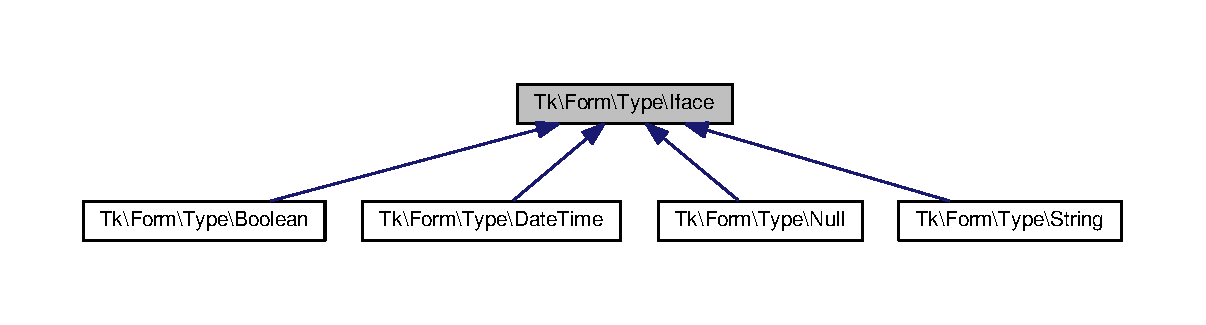
\includegraphics[width=350pt]{classTk_1_1Form_1_1Type_1_1Iface__inherit__graph}
\end{center}
\end{figure}
\subsection*{Public Member Functions}
\begin{DoxyCompactItemize}
\item 
\hyperlink{classTk_1_1Form_1_1Type_1_1Iface_ab7690bac7c47ccf3cb6c7cc8a6f02a99}{get\+Field} ()
\item 
\hyperlink{classTk_1_1Form_1_1Type_1_1Iface_a877c61a1d88fa32b28e4b87ed884c8ce}{set\+Field} (\$field)
\item 
\hyperlink{classTk_1_1Form_1_1Type_1_1Iface_a762247cf50d37305e4588c6b1edc5ed1}{set\+Value} (\$value)
\item 
\hyperlink{classTk_1_1Form_1_1Type_1_1Iface_a9ff099989b946924a7f79d05b91486dd}{get\+Value} ()
\item 
\hyperlink{classTk_1_1Form_1_1Type_1_1Iface_ac631bcfcb29a7f035de5e23d273f73fc}{get\+Text\+Value} ()
\item 
\hyperlink{classTk_1_1Form_1_1Type_1_1Iface_ab800a82de047293e6effb48815571b72}{to\+Type} (\$array)
\item 
\hyperlink{classTk_1_1Form_1_1Type_1_1Iface_a4d3b2fe521caa3364d61d7f9cee43246}{to\+Text} (\$array)
\item 
\hyperlink{classTk_1_1Form_1_1Type_1_1Iface_a145f18a1a3aee233c693c0258b13f61d}{load\+From\+Text} (\$str\+Arr)
\item 
\hyperlink{classTk_1_1Form_1_1Type_1_1Iface_ac641a4310b506486a87194eb22172c53}{load\+From\+Type} (\$type\+Arr)
\end{DoxyCompactItemize}
\subsection*{Protected Attributes}
\begin{DoxyCompactItemize}
\item 
\hypertarget{classTk_1_1Form_1_1Type_1_1Iface_ae61588b1bae22ef01c9958f8459f9d72}{{\bfseries \$field} = null}\label{classTk_1_1Form_1_1Type_1_1Iface_ae61588b1bae22ef01c9958f8459f9d72}

\item 
\hypertarget{classTk_1_1Form_1_1Type_1_1Iface_a05bf66cea1de20deae610e38cb5b480c}{{\bfseries \$text\+Value} = array()}\label{classTk_1_1Form_1_1Type_1_1Iface_a05bf66cea1de20deae610e38cb5b480c}

\item 
\hypertarget{classTk_1_1Form_1_1Type_1_1Iface_ae6bec8a3a6be771e90cfa8ab256a6166}{{\bfseries \$type\+Value} = null}\label{classTk_1_1Form_1_1Type_1_1Iface_ae6bec8a3a6be771e90cfa8ab256a6166}

\end{DoxyCompactItemize}


\subsection{Detailed Description}
A type object converts form element values to required types.

\begin{DoxyAuthor}{Author}
Michael Mifsud \href{mailto:info@tropotek.com}{\tt info@tropotek.\+com} \hyperlink{}{Copyright 2015 Michael Mifsud }
\end{DoxyAuthor}


\subsection{Member Function Documentation}
\hypertarget{classTk_1_1Form_1_1Type_1_1Iface_ab7690bac7c47ccf3cb6c7cc8a6f02a99}{\index{Tk\+::\+Form\+::\+Type\+::\+Iface@{Tk\+::\+Form\+::\+Type\+::\+Iface}!get\+Field@{get\+Field}}
\index{get\+Field@{get\+Field}!Tk\+::\+Form\+::\+Type\+::\+Iface@{Tk\+::\+Form\+::\+Type\+::\+Iface}}
\subsubsection[{get\+Field}]{\setlength{\rightskip}{0pt plus 5cm}Tk\textbackslash{}\+Form\textbackslash{}\+Type\textbackslash{}\+Iface\+::get\+Field (
\begin{DoxyParamCaption}
{}
\end{DoxyParamCaption}
)}}\label{classTk_1_1Form_1_1Type_1_1Iface_ab7690bac7c47ccf3cb6c7cc8a6f02a99}
\begin{DoxyReturn}{Returns}
Field 
\end{DoxyReturn}
\hypertarget{classTk_1_1Form_1_1Type_1_1Iface_ac631bcfcb29a7f035de5e23d273f73fc}{\index{Tk\+::\+Form\+::\+Type\+::\+Iface@{Tk\+::\+Form\+::\+Type\+::\+Iface}!get\+Text\+Value@{get\+Text\+Value}}
\index{get\+Text\+Value@{get\+Text\+Value}!Tk\+::\+Form\+::\+Type\+::\+Iface@{Tk\+::\+Form\+::\+Type\+::\+Iface}}
\subsubsection[{get\+Text\+Value}]{\setlength{\rightskip}{0pt plus 5cm}Tk\textbackslash{}\+Form\textbackslash{}\+Type\textbackslash{}\+Iface\+::get\+Text\+Value (
\begin{DoxyParamCaption}
{}
\end{DoxyParamCaption}
)}}\label{classTk_1_1Form_1_1Type_1_1Iface_ac631bcfcb29a7f035de5e23d273f73fc}
Return the field values array Override this method for more complex types.

Generally this array has the field name and a value like so\+: array('field1' =$>$ 'Value1') but for more complex fields like a map we can return an array like\+: array('map\+Lat' =$>$ '0.\+0', 'map\+Lng' =$>$ 0.\+0, 'map\+Zoom' =$>$ 0)

\begin{DoxyReturn}{Returns}
array 
\end{DoxyReturn}
\hypertarget{classTk_1_1Form_1_1Type_1_1Iface_a9ff099989b946924a7f79d05b91486dd}{\index{Tk\+::\+Form\+::\+Type\+::\+Iface@{Tk\+::\+Form\+::\+Type\+::\+Iface}!get\+Value@{get\+Value}}
\index{get\+Value@{get\+Value}!Tk\+::\+Form\+::\+Type\+::\+Iface@{Tk\+::\+Form\+::\+Type\+::\+Iface}}
\subsubsection[{get\+Value}]{\setlength{\rightskip}{0pt plus 5cm}Tk\textbackslash{}\+Form\textbackslash{}\+Type\textbackslash{}\+Iface\+::get\+Value (
\begin{DoxyParamCaption}
{}
\end{DoxyParamCaption}
)}}\label{classTk_1_1Form_1_1Type_1_1Iface_a9ff099989b946924a7f79d05b91486dd}
Get the field value based on its type.

\begin{DoxyReturn}{Returns}
mixed 
\end{DoxyReturn}
\hypertarget{classTk_1_1Form_1_1Type_1_1Iface_a145f18a1a3aee233c693c0258b13f61d}{\index{Tk\+::\+Form\+::\+Type\+::\+Iface@{Tk\+::\+Form\+::\+Type\+::\+Iface}!load\+From\+Text@{load\+From\+Text}}
\index{load\+From\+Text@{load\+From\+Text}!Tk\+::\+Form\+::\+Type\+::\+Iface@{Tk\+::\+Form\+::\+Type\+::\+Iface}}
\subsubsection[{load\+From\+Text}]{\setlength{\rightskip}{0pt plus 5cm}Tk\textbackslash{}\+Form\textbackslash{}\+Type\textbackslash{}\+Iface\+::load\+From\+Text (
\begin{DoxyParamCaption}
\item[{}]{\$str\+Arr}
\end{DoxyParamCaption}
)}}\label{classTk_1_1Form_1_1Type_1_1Iface_a145f18a1a3aee233c693c0258b13f61d}
Load the field value object from a data source array. This is usually, but not limited to, the \$\+\_\+\+R\+E\+Q\+U\+E\+S\+T \$\+\_\+\+G\+E\+T or \$\+\_\+\+P\+O\+S\+T array's

N\+O\+T\+E\+: Override this method if you are using multiple fields


\begin{DoxyParams}[1]{Parameters}
array & {\em \$str\+Arr} & \\
\hline
\end{DoxyParams}
\begin{DoxyReturn}{Returns}
\$this 
\end{DoxyReturn}
\hypertarget{classTk_1_1Form_1_1Type_1_1Iface_ac641a4310b506486a87194eb22172c53}{\index{Tk\+::\+Form\+::\+Type\+::\+Iface@{Tk\+::\+Form\+::\+Type\+::\+Iface}!load\+From\+Type@{load\+From\+Type}}
\index{load\+From\+Type@{load\+From\+Type}!Tk\+::\+Form\+::\+Type\+::\+Iface@{Tk\+::\+Form\+::\+Type\+::\+Iface}}
\subsubsection[{load\+From\+Type}]{\setlength{\rightskip}{0pt plus 5cm}Tk\textbackslash{}\+Form\textbackslash{}\+Type\textbackslash{}\+Iface\+::load\+From\+Type (
\begin{DoxyParamCaption}
\item[{}]{\$type\+Arr}
\end{DoxyParamCaption}
)}}\label{classTk_1_1Form_1_1Type_1_1Iface_ac641a4310b506486a87194eb22172c53}
This array will have objects that need to be converted to strings from their complex types

N\+O\+T\+E\+: Override this method if you are using multiple complex types.


\begin{DoxyParams}[1]{Parameters}
array & {\em \$type\+Arr} & \\
\hline
\end{DoxyParams}
\begin{DoxyReturn}{Returns}
\$this 
\end{DoxyReturn}
\hypertarget{classTk_1_1Form_1_1Type_1_1Iface_a877c61a1d88fa32b28e4b87ed884c8ce}{\index{Tk\+::\+Form\+::\+Type\+::\+Iface@{Tk\+::\+Form\+::\+Type\+::\+Iface}!set\+Field@{set\+Field}}
\index{set\+Field@{set\+Field}!Tk\+::\+Form\+::\+Type\+::\+Iface@{Tk\+::\+Form\+::\+Type\+::\+Iface}}
\subsubsection[{set\+Field}]{\setlength{\rightskip}{0pt plus 5cm}Tk\textbackslash{}\+Form\textbackslash{}\+Type\textbackslash{}\+Iface\+::set\+Field (
\begin{DoxyParamCaption}
\item[{}]{\$field}
\end{DoxyParamCaption}
)}}\label{classTk_1_1Form_1_1Type_1_1Iface_a877c61a1d88fa32b28e4b87ed884c8ce}

\begin{DoxyParams}[1]{Parameters}
Field\textbackslash{}\+Iface & {\em \$field} & \\
\hline
\end{DoxyParams}
\begin{DoxyReturn}{Returns}
\$this 
\end{DoxyReturn}
\hypertarget{classTk_1_1Form_1_1Type_1_1Iface_a762247cf50d37305e4588c6b1edc5ed1}{\index{Tk\+::\+Form\+::\+Type\+::\+Iface@{Tk\+::\+Form\+::\+Type\+::\+Iface}!set\+Value@{set\+Value}}
\index{set\+Value@{set\+Value}!Tk\+::\+Form\+::\+Type\+::\+Iface@{Tk\+::\+Form\+::\+Type\+::\+Iface}}
\subsubsection[{set\+Value}]{\setlength{\rightskip}{0pt plus 5cm}Tk\textbackslash{}\+Form\textbackslash{}\+Type\textbackslash{}\+Iface\+::set\+Value (
\begin{DoxyParamCaption}
\item[{}]{\$value}
\end{DoxyParamCaption}
)}}\label{classTk_1_1Form_1_1Type_1_1Iface_a762247cf50d37305e4588c6b1edc5ed1}
Set the complex type value of the field,

This method expects the value to be in its fields complex type,

I\+E\+:  The value must be a number (14)  The value must be a  object


\begin{DoxyParams}[1]{Parameters}
mixed & {\em \$value} & \\
\hline
\end{DoxyParams}
\begin{DoxyReturn}{Returns}
\$this 
\end{DoxyReturn}
\hypertarget{classTk_1_1Form_1_1Type_1_1Iface_a4d3b2fe521caa3364d61d7f9cee43246}{\index{Tk\+::\+Form\+::\+Type\+::\+Iface@{Tk\+::\+Form\+::\+Type\+::\+Iface}!to\+Text@{to\+Text}}
\index{to\+Text@{to\+Text}!Tk\+::\+Form\+::\+Type\+::\+Iface@{Tk\+::\+Form\+::\+Type\+::\+Iface}}
\subsubsection[{to\+Text}]{\setlength{\rightskip}{0pt plus 5cm}Tk\textbackslash{}\+Form\textbackslash{}\+Type\textbackslash{}\+Iface\+::to\+Text (
\begin{DoxyParamCaption}
\item[{}]{\$array}
\end{DoxyParamCaption}
)\hspace{0.3cm}{\ttfamily [abstract]}}}\label{classTk_1_1Form_1_1Type_1_1Iface_a4d3b2fe521caa3364d61d7f9cee43246}
Convert the field's complex type into a string for the required field


\begin{DoxyParams}[1]{Parameters}
array | \textbackslash{}std\+Class & {\em \$array} & \\
\hline
\end{DoxyParams}
\begin{DoxyReturn}{Returns}
string 
\end{DoxyReturn}
\hypertarget{classTk_1_1Form_1_1Type_1_1Iface_ab800a82de047293e6effb48815571b72}{\index{Tk\+::\+Form\+::\+Type\+::\+Iface@{Tk\+::\+Form\+::\+Type\+::\+Iface}!to\+Type@{to\+Type}}
\index{to\+Type@{to\+Type}!Tk\+::\+Form\+::\+Type\+::\+Iface@{Tk\+::\+Form\+::\+Type\+::\+Iface}}
\subsubsection[{to\+Type}]{\setlength{\rightskip}{0pt plus 5cm}Tk\textbackslash{}\+Form\textbackslash{}\+Type\textbackslash{}\+Iface\+::to\+Type (
\begin{DoxyParamCaption}
\item[{}]{\$array}
\end{DoxyParamCaption}
)\hspace{0.3cm}{\ttfamily [abstract]}}}\label{classTk_1_1Form_1_1Type_1_1Iface_ab800a82de047293e6effb48815571b72}
Convert the basic form submitted string field value into its correct complex type.


\begin{DoxyParams}[1]{Parameters}
array | \textbackslash{}std\+Class & {\em \$array} & \\
\hline
\end{DoxyParams}
\begin{DoxyReturn}{Returns}
mixed 
\end{DoxyReturn}


The documentation for this class was generated from the following file\+:\begin{DoxyCompactItemize}
\item 
vendor/ttek/tk-\/form/\+Tk/\+Form/\+Type/Iface.\+php\end{DoxyCompactItemize}

\hypertarget{classTk_1_1Form_1_1Field_1_1Iface}{\section{Tk\textbackslash{}Form\textbackslash{}Field\textbackslash{}Iface Class Reference}
\label{classTk_1_1Form_1_1Field_1_1Iface}\index{Tk\textbackslash{}\+Form\textbackslash{}\+Field\textbackslash{}\+Iface@{Tk\textbackslash{}\+Form\textbackslash{}\+Field\textbackslash{}\+Iface}}
}


Inheritance diagram for Tk\textbackslash{}Form\textbackslash{}Field\textbackslash{}Iface\+:\nopagebreak
\begin{figure}[H]
\begin{center}
\leavevmode
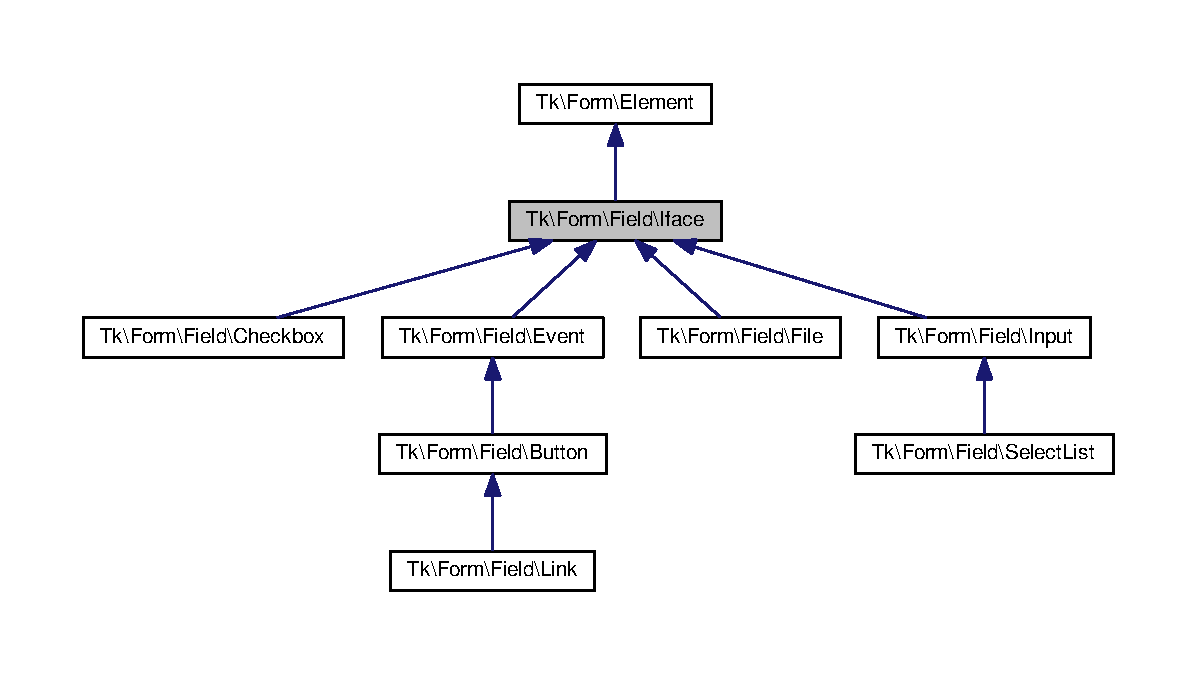
\includegraphics[width=350pt]{classTk_1_1Form_1_1Field_1_1Iface__inherit__graph}
\end{center}
\end{figure}
\subsection*{Public Member Functions}
\begin{DoxyCompactItemize}
\item 
\hyperlink{classTk_1_1Form_1_1Field_1_1Iface_a9453447f3b3bfd3224c405fc7891164f}{\+\_\+\+\_\+construct} (\$name, \hyperlink{classTk_1_1Form_1_1Type_1_1Iface}{Type\textbackslash{}\+Iface} \$type=null)
\item 
\hyperlink{classTk_1_1Form_1_1Field_1_1Iface_aeb681a399b302d8e59c3bfa9ffaad8f6}{get\+Type} ()
\item 
\hyperlink{classTk_1_1Form_1_1Field_1_1Iface_a95d310990b818c6ba2642f7a1d259d17}{set\+Type} (\$type)
\item 
\hyperlink{classTk_1_1Form_1_1Field_1_1Iface_aed87bd5d6a5340110e720eac165e293b}{set\+Name} (\$name)
\item 
\hyperlink{classTk_1_1Form_1_1Field_1_1Iface_a049c1bf0b5dc2ffa86f2a5923da885c4}{set\+Form} (\hyperlink{classTk_1_1Form}{Form} \$form)
\item 
\hyperlink{classTk_1_1Form_1_1Field_1_1Iface_abdf6272573e78a59305eacbe63ff91d8}{get\+Renderer} ()
\item 
\hyperlink{classTk_1_1Form_1_1Field_1_1Iface_a1f31fd814446382b6fdf9b2fda03075d}{set\+Renderer} (\$renderer)
\item 
\hyperlink{classTk_1_1Form_1_1Field_1_1Iface_ad52b8e4418c37eb5fb4647e069342098}{is\+Required} ()
\item 
\hyperlink{classTk_1_1Form_1_1Field_1_1Iface_aa4d7d60b8a821fe4d2c58eb7ed425d1b}{set\+Required} (\$required)
\item 
\hyperlink{classTk_1_1Form_1_1Field_1_1Iface_a2028dc86f15fc36fe16a49947ce37372}{get\+Label} ()
\item 
\hyperlink{classTk_1_1Form_1_1Field_1_1Iface_a1c881f3ad731b280e6ee08e74b53971a}{set\+Label} (\$str)
\item 
\hyperlink{classTk_1_1Form_1_1Field_1_1Iface_a634bd8c5c658bd59d561f412e50d94da}{set\+Notes} (\$html)
\item 
\hyperlink{classTk_1_1Form_1_1Field_1_1Iface_ab1d30e73d0b521e2f6faa175db0ff8ee}{get\+Notes} ()
\item 
\hyperlink{classTk_1_1Form_1_1Field_1_1Iface_aa2c66caa4340ea6d622801621acb6f11}{is\+Array} ()
\item 
\hyperlink{classTk_1_1Form_1_1Field_1_1Iface_a952b97c0a1505dffe1f708cb4b91cc2e}{set\+Value} (\$value)
\item 
\hyperlink{classTk_1_1Form_1_1Field_1_1Iface_a18558c8f8f720774e0eff59d3ced5d30}{get\+Value} ()
\end{DoxyCompactItemize}
\subsection*{Static Public Member Functions}
\begin{DoxyCompactItemize}
\item 
static \hyperlink{classTk_1_1Form_1_1Field_1_1Iface_a3e56843fc0f56856485f5b99c59e7425}{make\+Label} (\$name)
\end{DoxyCompactItemize}
\subsection*{Protected Member Functions}
\begin{DoxyCompactItemize}
\item 
\hyperlink{classTk_1_1Form_1_1Field_1_1Iface_acae9d96d10be302b5af48f2ae11633a9}{make\+Id} (\$prepend= 'fid\+\_\+')
\end{DoxyCompactItemize}
\subsection*{Protected Attributes}
\begin{DoxyCompactItemize}
\item 
\hypertarget{classTk_1_1Form_1_1Field_1_1Iface_a99321b47c888e922b1b269ab3da819e6}{{\bfseries \$required} = false}\label{classTk_1_1Form_1_1Field_1_1Iface_a99321b47c888e922b1b269ab3da819e6}

\item 
\hypertarget{classTk_1_1Form_1_1Field_1_1Iface_aa217965a0440d30fb8c2e0ef752e8ac8}{{\bfseries \$label} = ''}\label{classTk_1_1Form_1_1Field_1_1Iface_aa217965a0440d30fb8c2e0ef752e8ac8}

\item 
\hypertarget{classTk_1_1Form_1_1Field_1_1Iface_a8befa24f089af49b07f96fc58d0942cc}{{\bfseries \$notes} = ''}\label{classTk_1_1Form_1_1Field_1_1Iface_a8befa24f089af49b07f96fc58d0942cc}

\item 
\hypertarget{classTk_1_1Form_1_1Field_1_1Iface_a293a78923c3f075d7da5e35222de0fbb}{{\bfseries \$array\+Field} = false}\label{classTk_1_1Form_1_1Field_1_1Iface_a293a78923c3f075d7da5e35222de0fbb}

\item 
\hypertarget{classTk_1_1Form_1_1Field_1_1Iface_a0006eca554e380975397befac780bf22}{{\bfseries \$type} = null}\label{classTk_1_1Form_1_1Field_1_1Iface_a0006eca554e380975397befac780bf22}

\item 
\hypertarget{classTk_1_1Form_1_1Field_1_1Iface_a4c412caeb92991d723730df7cb2e20b6}{{\bfseries \$renderer} = null}\label{classTk_1_1Form_1_1Field_1_1Iface_a4c412caeb92991d723730df7cb2e20b6}

\end{DoxyCompactItemize}


\subsection{Detailed Description}
Class \hyperlink{classTk_1_1Form_1_1Field_1_1Iface}{Iface}

\begin{DoxyAuthor}{Author}
Michael Mifsud \href{mailto:info@tropotek.com}{\tt info@tropotek.\+com} \hyperlink{}{Copyright 2015 Michael Mifsud }
\end{DoxyAuthor}


\subsection{Constructor \& Destructor Documentation}
\hypertarget{classTk_1_1Form_1_1Field_1_1Iface_a9453447f3b3bfd3224c405fc7891164f}{\index{Tk\+::\+Form\+::\+Field\+::\+Iface@{Tk\+::\+Form\+::\+Field\+::\+Iface}!\+\_\+\+\_\+construct@{\+\_\+\+\_\+construct}}
\index{\+\_\+\+\_\+construct@{\+\_\+\+\_\+construct}!Tk\+::\+Form\+::\+Field\+::\+Iface@{Tk\+::\+Form\+::\+Field\+::\+Iface}}
\subsubsection[{\+\_\+\+\_\+construct}]{\setlength{\rightskip}{0pt plus 5cm}Tk\textbackslash{}\+Form\textbackslash{}\+Field\textbackslash{}\+Iface\+::\+\_\+\+\_\+construct (
\begin{DoxyParamCaption}
\item[{}]{\$name, }
\item[{{\bf Type\textbackslash{}\+Iface}}]{\$type = {\ttfamily null}}
\end{DoxyParamCaption}
)}}\label{classTk_1_1Form_1_1Field_1_1Iface_a9453447f3b3bfd3224c405fc7891164f}
\+\_\+\+\_\+construct


\begin{DoxyParams}[1]{Parameters}
string & {\em \$name} & \\
\hline
Type\textbackslash{}\+Iface | null & {\em \$type} & \\
\hline
\end{DoxyParams}

\begin{DoxyExceptions}{Exceptions}
{\em \hyperlink{classTk_1_1Form_1_1Exception}{Exception}} & \\
\hline
\end{DoxyExceptions}


\subsection{Member Function Documentation}
\hypertarget{classTk_1_1Form_1_1Field_1_1Iface_a2028dc86f15fc36fe16a49947ce37372}{\index{Tk\+::\+Form\+::\+Field\+::\+Iface@{Tk\+::\+Form\+::\+Field\+::\+Iface}!get\+Label@{get\+Label}}
\index{get\+Label@{get\+Label}!Tk\+::\+Form\+::\+Field\+::\+Iface@{Tk\+::\+Form\+::\+Field\+::\+Iface}}
\subsubsection[{get\+Label}]{\setlength{\rightskip}{0pt plus 5cm}Tk\textbackslash{}\+Form\textbackslash{}\+Field\textbackslash{}\+Iface\+::get\+Label (
\begin{DoxyParamCaption}
{}
\end{DoxyParamCaption}
)}}\label{classTk_1_1Form_1_1Field_1_1Iface_a2028dc86f15fc36fe16a49947ce37372}
Get the label of this field

\begin{DoxyReturn}{Returns}
string 
\end{DoxyReturn}
\hypertarget{classTk_1_1Form_1_1Field_1_1Iface_ab1d30e73d0b521e2f6faa175db0ff8ee}{\index{Tk\+::\+Form\+::\+Field\+::\+Iface@{Tk\+::\+Form\+::\+Field\+::\+Iface}!get\+Notes@{get\+Notes}}
\index{get\+Notes@{get\+Notes}!Tk\+::\+Form\+::\+Field\+::\+Iface@{Tk\+::\+Form\+::\+Field\+::\+Iface}}
\subsubsection[{get\+Notes}]{\setlength{\rightskip}{0pt plus 5cm}Tk\textbackslash{}\+Form\textbackslash{}\+Field\textbackslash{}\+Iface\+::get\+Notes (
\begin{DoxyParamCaption}
{}
\end{DoxyParamCaption}
)}}\label{classTk_1_1Form_1_1Field_1_1Iface_ab1d30e73d0b521e2f6faa175db0ff8ee}
Get any notes on this element

\begin{DoxyReturn}{Returns}
string 
\end{DoxyReturn}
\hypertarget{classTk_1_1Form_1_1Field_1_1Iface_abdf6272573e78a59305eacbe63ff91d8}{\index{Tk\+::\+Form\+::\+Field\+::\+Iface@{Tk\+::\+Form\+::\+Field\+::\+Iface}!get\+Renderer@{get\+Renderer}}
\index{get\+Renderer@{get\+Renderer}!Tk\+::\+Form\+::\+Field\+::\+Iface@{Tk\+::\+Form\+::\+Field\+::\+Iface}}
\subsubsection[{get\+Renderer}]{\setlength{\rightskip}{0pt plus 5cm}Tk\textbackslash{}\+Form\textbackslash{}\+Field\textbackslash{}\+Iface\+::get\+Renderer (
\begin{DoxyParamCaption}
{}
\end{DoxyParamCaption}
)}}\label{classTk_1_1Form_1_1Field_1_1Iface_abdf6272573e78a59305eacbe63ff91d8}
Get the renderer object

\begin{DoxyReturn}{Returns}
mixed 
\end{DoxyReturn}
\hypertarget{classTk_1_1Form_1_1Field_1_1Iface_aeb681a399b302d8e59c3bfa9ffaad8f6}{\index{Tk\+::\+Form\+::\+Field\+::\+Iface@{Tk\+::\+Form\+::\+Field\+::\+Iface}!get\+Type@{get\+Type}}
\index{get\+Type@{get\+Type}!Tk\+::\+Form\+::\+Field\+::\+Iface@{Tk\+::\+Form\+::\+Field\+::\+Iface}}
\subsubsection[{get\+Type}]{\setlength{\rightskip}{0pt plus 5cm}Tk\textbackslash{}\+Form\textbackslash{}\+Field\textbackslash{}\+Iface\+::get\+Type (
\begin{DoxyParamCaption}
{}
\end{DoxyParamCaption}
)}}\label{classTk_1_1Form_1_1Field_1_1Iface_aeb681a399b302d8e59c3bfa9ffaad8f6}
\begin{DoxyReturn}{Returns}
Type 
\end{DoxyReturn}
\hypertarget{classTk_1_1Form_1_1Field_1_1Iface_a18558c8f8f720774e0eff59d3ced5d30}{\index{Tk\+::\+Form\+::\+Field\+::\+Iface@{Tk\+::\+Form\+::\+Field\+::\+Iface}!get\+Value@{get\+Value}}
\index{get\+Value@{get\+Value}!Tk\+::\+Form\+::\+Field\+::\+Iface@{Tk\+::\+Form\+::\+Field\+::\+Iface}}
\subsubsection[{get\+Value}]{\setlength{\rightskip}{0pt plus 5cm}Tk\textbackslash{}\+Form\textbackslash{}\+Field\textbackslash{}\+Iface\+::get\+Value (
\begin{DoxyParamCaption}
{}
\end{DoxyParamCaption}
)}}\label{classTk_1_1Form_1_1Field_1_1Iface_a18558c8f8f720774e0eff59d3ced5d30}
Get the field value based on its type.

\begin{DoxyReturn}{Returns}
mixed 
\end{DoxyReturn}
\hypertarget{classTk_1_1Form_1_1Field_1_1Iface_aa2c66caa4340ea6d622801621acb6f11}{\index{Tk\+::\+Form\+::\+Field\+::\+Iface@{Tk\+::\+Form\+::\+Field\+::\+Iface}!is\+Array@{is\+Array}}
\index{is\+Array@{is\+Array}!Tk\+::\+Form\+::\+Field\+::\+Iface@{Tk\+::\+Form\+::\+Field\+::\+Iface}}
\subsubsection[{is\+Array}]{\setlength{\rightskip}{0pt plus 5cm}Tk\textbackslash{}\+Form\textbackslash{}\+Field\textbackslash{}\+Iface\+::is\+Array (
\begin{DoxyParamCaption}
{}
\end{DoxyParamCaption}
)}}\label{classTk_1_1Form_1_1Field_1_1Iface_aa2c66caa4340ea6d622801621acb6f11}
Does this fields data come as an array. If the name ends in \mbox{[}\mbox{]} then it will be flagged as an array\+Field.

E\+G\+: name={\ttfamily name\mbox{[}\mbox{]}}

\begin{DoxyReturn}{Returns}
boolean 
\end{DoxyReturn}
\hypertarget{classTk_1_1Form_1_1Field_1_1Iface_ad52b8e4418c37eb5fb4647e069342098}{\index{Tk\+::\+Form\+::\+Field\+::\+Iface@{Tk\+::\+Form\+::\+Field\+::\+Iface}!is\+Required@{is\+Required}}
\index{is\+Required@{is\+Required}!Tk\+::\+Form\+::\+Field\+::\+Iface@{Tk\+::\+Form\+::\+Field\+::\+Iface}}
\subsubsection[{is\+Required}]{\setlength{\rightskip}{0pt plus 5cm}Tk\textbackslash{}\+Form\textbackslash{}\+Field\textbackslash{}\+Iface\+::is\+Required (
\begin{DoxyParamCaption}
{}
\end{DoxyParamCaption}
)}}\label{classTk_1_1Form_1_1Field_1_1Iface_ad52b8e4418c37eb5fb4647e069342098}
is\+Required

\begin{DoxyReturn}{Returns}
boolean 
\end{DoxyReturn}
\hypertarget{classTk_1_1Form_1_1Field_1_1Iface_acae9d96d10be302b5af48f2ae11633a9}{\index{Tk\+::\+Form\+::\+Field\+::\+Iface@{Tk\+::\+Form\+::\+Field\+::\+Iface}!make\+Id@{make\+Id}}
\index{make\+Id@{make\+Id}!Tk\+::\+Form\+::\+Field\+::\+Iface@{Tk\+::\+Form\+::\+Field\+::\+Iface}}
\subsubsection[{make\+Id}]{\setlength{\rightskip}{0pt plus 5cm}Tk\textbackslash{}\+Form\textbackslash{}\+Field\textbackslash{}\+Iface\+::make\+Id (
\begin{DoxyParamCaption}
\item[{}]{\$prepend = {\ttfamily 'fid\+\_\+'}}
\end{DoxyParamCaption}
)\hspace{0.3cm}{\ttfamily [protected]}}}\label{classTk_1_1Form_1_1Field_1_1Iface_acae9d96d10be302b5af48f2ae11633a9}
Get the unique name for this field


\begin{DoxyParams}[1]{Parameters}
string & {\em \$prepend} & \\
\hline
\end{DoxyParams}
\begin{DoxyReturn}{Returns}
string 
\end{DoxyReturn}
\hypertarget{classTk_1_1Form_1_1Field_1_1Iface_a3e56843fc0f56856485f5b99c59e7425}{\index{Tk\+::\+Form\+::\+Field\+::\+Iface@{Tk\+::\+Form\+::\+Field\+::\+Iface}!make\+Label@{make\+Label}}
\index{make\+Label@{make\+Label}!Tk\+::\+Form\+::\+Field\+::\+Iface@{Tk\+::\+Form\+::\+Field\+::\+Iface}}
\subsubsection[{make\+Label}]{\setlength{\rightskip}{0pt plus 5cm}static Tk\textbackslash{}\+Form\textbackslash{}\+Field\textbackslash{}\+Iface\+::make\+Label (
\begin{DoxyParamCaption}
\item[{}]{\$name}
\end{DoxyParamCaption}
)\hspace{0.3cm}{\ttfamily [static]}}}\label{classTk_1_1Form_1_1Field_1_1Iface_a3e56843fc0f56856485f5b99c59e7425}
Create a label from a name string The default label uses the name (E\+G\+: {\ttfamily field\+Name\+Select} -\/$>$ {\ttfamily Field Name Select})


\begin{DoxyParams}[1]{Parameters}
string & {\em \$name} & \\
\hline
\end{DoxyParams}
\begin{DoxyReturn}{Returns}
string 
\end{DoxyReturn}
\hypertarget{classTk_1_1Form_1_1Field_1_1Iface_a049c1bf0b5dc2ffa86f2a5923da885c4}{\index{Tk\+::\+Form\+::\+Field\+::\+Iface@{Tk\+::\+Form\+::\+Field\+::\+Iface}!set\+Form@{set\+Form}}
\index{set\+Form@{set\+Form}!Tk\+::\+Form\+::\+Field\+::\+Iface@{Tk\+::\+Form\+::\+Field\+::\+Iface}}
\subsubsection[{set\+Form}]{\setlength{\rightskip}{0pt plus 5cm}Tk\textbackslash{}\+Form\textbackslash{}\+Field\textbackslash{}\+Iface\+::set\+Form (
\begin{DoxyParamCaption}
\item[{{\bf Form}}]{\$form}
\end{DoxyParamCaption}
)}}\label{classTk_1_1Form_1_1Field_1_1Iface_a049c1bf0b5dc2ffa86f2a5923da885c4}
Set the form for this element


\begin{DoxyParams}[1]{Parameters}
\hyperlink{classTk_1_1Form}{Form} & {\em \$form} & \\
\hline
\end{DoxyParams}
\begin{DoxyReturn}{Returns}
\$this 
\end{DoxyReturn}
\hypertarget{classTk_1_1Form_1_1Field_1_1Iface_a1c881f3ad731b280e6ee08e74b53971a}{\index{Tk\+::\+Form\+::\+Field\+::\+Iface@{Tk\+::\+Form\+::\+Field\+::\+Iface}!set\+Label@{set\+Label}}
\index{set\+Label@{set\+Label}!Tk\+::\+Form\+::\+Field\+::\+Iface@{Tk\+::\+Form\+::\+Field\+::\+Iface}}
\subsubsection[{set\+Label}]{\setlength{\rightskip}{0pt plus 5cm}Tk\textbackslash{}\+Form\textbackslash{}\+Field\textbackslash{}\+Iface\+::set\+Label (
\begin{DoxyParamCaption}
\item[{}]{\$str}
\end{DoxyParamCaption}
)}}\label{classTk_1_1Form_1_1Field_1_1Iface_a1c881f3ad731b280e6ee08e74b53971a}
Set the label of this field


\begin{DoxyParams}{Parameters}
{\em \$str} & \\
\hline
\end{DoxyParams}
\begin{DoxyReturn}{Returns}
\$this 
\end{DoxyReturn}
\hypertarget{classTk_1_1Form_1_1Field_1_1Iface_aed87bd5d6a5340110e720eac165e293b}{\index{Tk\+::\+Form\+::\+Field\+::\+Iface@{Tk\+::\+Form\+::\+Field\+::\+Iface}!set\+Name@{set\+Name}}
\index{set\+Name@{set\+Name}!Tk\+::\+Form\+::\+Field\+::\+Iface@{Tk\+::\+Form\+::\+Field\+::\+Iface}}
\subsubsection[{set\+Name}]{\setlength{\rightskip}{0pt plus 5cm}Tk\textbackslash{}\+Form\textbackslash{}\+Field\textbackslash{}\+Iface\+::set\+Name (
\begin{DoxyParamCaption}
\item[{}]{\$name}
\end{DoxyParamCaption}
)}}\label{classTk_1_1Form_1_1Field_1_1Iface_aed87bd5d6a5340110e720eac165e293b}
Set the name for this element

When using the element with an array name (E\+G\+: 'name\mbox{[}\mbox{]}') The '\mbox{[}\mbox{]}' are removed from the name but the is\+Array value is set to true.

N\+O\+T\+E\+: only single dimensional numbered arrays are supported, Multidimensional or named arrays are not. Invalid field name examples are\+: o 'name\mbox{[}key\mbox{]}' o 'name\mbox{[}\mbox{]}\mbox{[}\mbox{]}' o 'name\mbox{[}key\mbox{]}\mbox{[}\mbox{]}'


\begin{DoxyParams}{Parameters}
{\em \$name} & \\
\hline
\end{DoxyParams}
\begin{DoxyReturn}{Returns}
\$this 
\end{DoxyReturn}

\begin{DoxyExceptions}{Exceptions}
{\em \hyperlink{classTk_1_1Form_1_1Exception}{Exception}} & \\
\hline
\end{DoxyExceptions}
\hypertarget{classTk_1_1Form_1_1Field_1_1Iface_a634bd8c5c658bd59d561f412e50d94da}{\index{Tk\+::\+Form\+::\+Field\+::\+Iface@{Tk\+::\+Form\+::\+Field\+::\+Iface}!set\+Notes@{set\+Notes}}
\index{set\+Notes@{set\+Notes}!Tk\+::\+Form\+::\+Field\+::\+Iface@{Tk\+::\+Form\+::\+Field\+::\+Iface}}
\subsubsection[{set\+Notes}]{\setlength{\rightskip}{0pt plus 5cm}Tk\textbackslash{}\+Form\textbackslash{}\+Field\textbackslash{}\+Iface\+::set\+Notes (
\begin{DoxyParamCaption}
\item[{}]{\$html}
\end{DoxyParamCaption}
)}}\label{classTk_1_1Form_1_1Field_1_1Iface_a634bd8c5c658bd59d561f412e50d94da}
Set the notes html


\begin{DoxyParams}[1]{Parameters}
string & {\em \$html} & \\
\hline
\end{DoxyParams}
\begin{DoxyReturn}{Returns}
\$this 
\end{DoxyReturn}
\hypertarget{classTk_1_1Form_1_1Field_1_1Iface_a1f31fd814446382b6fdf9b2fda03075d}{\index{Tk\+::\+Form\+::\+Field\+::\+Iface@{Tk\+::\+Form\+::\+Field\+::\+Iface}!set\+Renderer@{set\+Renderer}}
\index{set\+Renderer@{set\+Renderer}!Tk\+::\+Form\+::\+Field\+::\+Iface@{Tk\+::\+Form\+::\+Field\+::\+Iface}}
\subsubsection[{set\+Renderer}]{\setlength{\rightskip}{0pt plus 5cm}Tk\textbackslash{}\+Form\textbackslash{}\+Field\textbackslash{}\+Iface\+::set\+Renderer (
\begin{DoxyParamCaption}
\item[{}]{\$renderer}
\end{DoxyParamCaption}
)}}\label{classTk_1_1Form_1_1Field_1_1Iface_a1f31fd814446382b6fdf9b2fda03075d}
Set the renderer object


\begin{DoxyParams}[1]{Parameters}
mixed & {\em \$renderer} & \\
\hline
\end{DoxyParams}
\begin{DoxyReturn}{Returns}
\$this 
\end{DoxyReturn}
\hypertarget{classTk_1_1Form_1_1Field_1_1Iface_aa4d7d60b8a821fe4d2c58eb7ed425d1b}{\index{Tk\+::\+Form\+::\+Field\+::\+Iface@{Tk\+::\+Form\+::\+Field\+::\+Iface}!set\+Required@{set\+Required}}
\index{set\+Required@{set\+Required}!Tk\+::\+Form\+::\+Field\+::\+Iface@{Tk\+::\+Form\+::\+Field\+::\+Iface}}
\subsubsection[{set\+Required}]{\setlength{\rightskip}{0pt plus 5cm}Tk\textbackslash{}\+Form\textbackslash{}\+Field\textbackslash{}\+Iface\+::set\+Required (
\begin{DoxyParamCaption}
\item[{}]{\$required}
\end{DoxyParamCaption}
)}}\label{classTk_1_1Form_1_1Field_1_1Iface_aa4d7d60b8a821fe4d2c58eb7ed425d1b}
set\+Required


\begin{DoxyParams}[1]{Parameters}
boolean & {\em \$required} & \\
\hline
\end{DoxyParams}
\begin{DoxyReturn}{Returns}
\$this 
\end{DoxyReturn}
\hypertarget{classTk_1_1Form_1_1Field_1_1Iface_a95d310990b818c6ba2642f7a1d259d17}{\index{Tk\+::\+Form\+::\+Field\+::\+Iface@{Tk\+::\+Form\+::\+Field\+::\+Iface}!set\+Type@{set\+Type}}
\index{set\+Type@{set\+Type}!Tk\+::\+Form\+::\+Field\+::\+Iface@{Tk\+::\+Form\+::\+Field\+::\+Iface}}
\subsubsection[{set\+Type}]{\setlength{\rightskip}{0pt plus 5cm}Tk\textbackslash{}\+Form\textbackslash{}\+Field\textbackslash{}\+Iface\+::set\+Type (
\begin{DoxyParamCaption}
\item[{}]{\$type}
\end{DoxyParamCaption}
)}}\label{classTk_1_1Form_1_1Field_1_1Iface_a95d310990b818c6ba2642f7a1d259d17}

\begin{DoxyParams}[1]{Parameters}
Type\textbackslash{}\+Iface & {\em \$type} & \\
\hline
\end{DoxyParams}
\begin{DoxyReturn}{Returns}
\$this 
\end{DoxyReturn}
\hypertarget{classTk_1_1Form_1_1Field_1_1Iface_a952b97c0a1505dffe1f708cb4b91cc2e}{\index{Tk\+::\+Form\+::\+Field\+::\+Iface@{Tk\+::\+Form\+::\+Field\+::\+Iface}!set\+Value@{set\+Value}}
\index{set\+Value@{set\+Value}!Tk\+::\+Form\+::\+Field\+::\+Iface@{Tk\+::\+Form\+::\+Field\+::\+Iface}}
\subsubsection[{set\+Value}]{\setlength{\rightskip}{0pt plus 5cm}Tk\textbackslash{}\+Form\textbackslash{}\+Field\textbackslash{}\+Iface\+::set\+Value (
\begin{DoxyParamCaption}
\item[{}]{\$value}
\end{DoxyParamCaption}
)}}\label{classTk_1_1Form_1_1Field_1_1Iface_a952b97c0a1505dffe1f708cb4b91cc2e}
Set the complex type value of the field,


\begin{DoxyParams}[1]{Parameters}
mixed & {\em \$value} & \\
\hline
\end{DoxyParams}
\begin{DoxyReturn}{Returns}
\$this 
\end{DoxyReturn}


The documentation for this class was generated from the following file\+:\begin{DoxyCompactItemize}
\item 
vendor/ttek/tk-\/form/\+Tk/\+Form/\+Field/Iface.\+php\end{DoxyCompactItemize}

\hypertarget{classTk_1_1Composer_1_1Script_1_1Event_1_1InitProject}{\section{Tk\textbackslash{}Composer\textbackslash{}Script\textbackslash{}Event\textbackslash{}Init\+Project Class Reference}
\label{classTk_1_1Composer_1_1Script_1_1Event_1_1InitProject}\index{Tk\textbackslash{}\+Composer\textbackslash{}\+Script\textbackslash{}\+Event\textbackslash{}\+Init\+Project@{Tk\textbackslash{}\+Composer\textbackslash{}\+Script\textbackslash{}\+Event\textbackslash{}\+Init\+Project}}
}
\subsection*{Static Public Member Functions}
\begin{DoxyCompactItemize}
\item 
static \hyperlink{classTk_1_1Composer_1_1Script_1_1Event_1_1InitProject_acd00c2e59dbe837096c4c456e4e95982}{post\+Install} (Event \$event)
\item 
static \hyperlink{classTk_1_1Composer_1_1Script_1_1Event_1_1InitProject_a47c5fd63d49d586f731f80ba6c22ee0a}{post\+Update} (Event \$event)
\item 
static \hyperlink{classTk_1_1Composer_1_1Script_1_1Event_1_1InitProject_ae1669776278466460408f59bfa35c483}{init} (Event \$event)
\end{DoxyCompactItemize}


\subsection{Detailed Description}
Class \hyperlink{classTk_1_1Composer_1_1Script_1_1Event_1_1InitProject}{Init\+Project}

Default init\+Project installer class for the framework V2

\begin{DoxyAuthor}{Author}
Michael Mifsud \href{mailto:info@tropotek.com}{\tt info@tropotek.\+com} \hyperlink{}{Copyright 2007 Michael Mifsud }
\end{DoxyAuthor}


\subsection{Member Function Documentation}
\hypertarget{classTk_1_1Composer_1_1Script_1_1Event_1_1InitProject_ae1669776278466460408f59bfa35c483}{\index{Tk\+::\+Composer\+::\+Script\+::\+Event\+::\+Init\+Project@{Tk\+::\+Composer\+::\+Script\+::\+Event\+::\+Init\+Project}!init@{init}}
\index{init@{init}!Tk\+::\+Composer\+::\+Script\+::\+Event\+::\+Init\+Project@{Tk\+::\+Composer\+::\+Script\+::\+Event\+::\+Init\+Project}}
\subsubsection[{init}]{\setlength{\rightskip}{0pt plus 5cm}static Tk\textbackslash{}\+Composer\textbackslash{}\+Script\textbackslash{}\+Event\textbackslash{}\+Init\+Project\+::init (
\begin{DoxyParamCaption}
\item[{Event}]{\$event}
\end{DoxyParamCaption}
)\hspace{0.3cm}{\ttfamily [static]}}}\label{classTk_1_1Composer_1_1Script_1_1Event_1_1InitProject_ae1669776278466460408f59bfa35c483}

\begin{DoxyParams}[1]{Parameters}
Event & {\em \$event} & \\
\hline
\end{DoxyParams}
\hypertarget{classTk_1_1Composer_1_1Script_1_1Event_1_1InitProject_acd00c2e59dbe837096c4c456e4e95982}{\index{Tk\+::\+Composer\+::\+Script\+::\+Event\+::\+Init\+Project@{Tk\+::\+Composer\+::\+Script\+::\+Event\+::\+Init\+Project}!post\+Install@{post\+Install}}
\index{post\+Install@{post\+Install}!Tk\+::\+Composer\+::\+Script\+::\+Event\+::\+Init\+Project@{Tk\+::\+Composer\+::\+Script\+::\+Event\+::\+Init\+Project}}
\subsubsection[{post\+Install}]{\setlength{\rightskip}{0pt plus 5cm}static Tk\textbackslash{}\+Composer\textbackslash{}\+Script\textbackslash{}\+Event\textbackslash{}\+Init\+Project\+::post\+Install (
\begin{DoxyParamCaption}
\item[{Event}]{\$event}
\end{DoxyParamCaption}
)\hspace{0.3cm}{\ttfamily [static]}}}\label{classTk_1_1Composer_1_1Script_1_1Event_1_1InitProject_acd00c2e59dbe837096c4c456e4e95982}

\begin{DoxyParams}[1]{Parameters}
Event & {\em \$event} & \\
\hline
\end{DoxyParams}
\hypertarget{classTk_1_1Composer_1_1Script_1_1Event_1_1InitProject_a47c5fd63d49d586f731f80ba6c22ee0a}{\index{Tk\+::\+Composer\+::\+Script\+::\+Event\+::\+Init\+Project@{Tk\+::\+Composer\+::\+Script\+::\+Event\+::\+Init\+Project}!post\+Update@{post\+Update}}
\index{post\+Update@{post\+Update}!Tk\+::\+Composer\+::\+Script\+::\+Event\+::\+Init\+Project@{Tk\+::\+Composer\+::\+Script\+::\+Event\+::\+Init\+Project}}
\subsubsection[{post\+Update}]{\setlength{\rightskip}{0pt plus 5cm}static Tk\textbackslash{}\+Composer\textbackslash{}\+Script\textbackslash{}\+Event\textbackslash{}\+Init\+Project\+::post\+Update (
\begin{DoxyParamCaption}
\item[{Event}]{\$event}
\end{DoxyParamCaption}
)\hspace{0.3cm}{\ttfamily [static]}}}\label{classTk_1_1Composer_1_1Script_1_1Event_1_1InitProject_a47c5fd63d49d586f731f80ba6c22ee0a}

\begin{DoxyParams}[1]{Parameters}
Event & {\em \$event} & \\
\hline
\end{DoxyParams}


The documentation for this class was generated from the following file\+:\begin{DoxyCompactItemize}
\item 
vendor/ttek/tk-\/installers/\+Tk/\+Composer/\+Script/\+Event/Init\+Project.\+php\end{DoxyCompactItemize}

\hypertarget{classTk_1_1Form_1_1Field_1_1Input}{\section{Tk\textbackslash{}Form\textbackslash{}Field\textbackslash{}Input Class Reference}
\label{classTk_1_1Form_1_1Field_1_1Input}\index{Tk\textbackslash{}\+Form\textbackslash{}\+Field\textbackslash{}\+Input@{Tk\textbackslash{}\+Form\textbackslash{}\+Field\textbackslash{}\+Input}}
}


Inheritance diagram for Tk\textbackslash{}Form\textbackslash{}Field\textbackslash{}Input\+:\nopagebreak
\begin{figure}[H]
\begin{center}
\leavevmode
\includegraphics[width=204pt]{classTk_1_1Form_1_1Field_1_1Input__inherit__graph}
\end{center}
\end{figure}
\subsection*{Additional Inherited Members}


\subsection{Detailed Description}
Class Text

\begin{DoxyAuthor}{Author}
Michael Mifsud \href{mailto:info@tropotek.com}{\tt info@tropotek.\+com} \hyperlink{}{Copyright 2015 Michael Mifsud }
\end{DoxyAuthor}


The documentation for this class was generated from the following file\+:\begin{DoxyCompactItemize}
\item 
vendor/ttek/tk-\/form/\+Tk/\+Form/\+Field/Input.\+php\end{DoxyCompactItemize}

\hypertarget{classDom_1_1Form_1_1Input}{\section{Dom\textbackslash{}Form\textbackslash{}Input Class Reference}
\label{classDom_1_1Form_1_1Input}\index{Dom\textbackslash{}\+Form\textbackslash{}\+Input@{Dom\textbackslash{}\+Form\textbackslash{}\+Input}}
}


Inheritance diagram for Dom\textbackslash{}Form\textbackslash{}Input\+:\nopagebreak
\begin{figure}[H]
\begin{center}
\leavevmode
\includegraphics[width=182pt]{classDom_1_1Form_1_1Input__inherit__graph}
\end{center}
\end{figure}
\subsection*{Public Member Functions}
\begin{DoxyCompactItemize}
\item 
\hyperlink{classDom_1_1Form_1_1Input_a940675b13cb6baf05601e0880072bc5b}{set\+Checked} (\$b)
\item 
\hyperlink{classDom_1_1Form_1_1Input_aa822b93411df7db86d6bc0d99a255140}{is\+Checked} ()
\item 
\hyperlink{classDom_1_1Form_1_1Input_a95beded58548822c685f18df625eee88}{set\+Value} (\$value)
\item 
\hyperlink{classDom_1_1Form_1_1Input_a9f426e01159412d88c6ed1ac3d71d883}{get\+Value} ()
\end{DoxyCompactItemize}
\subsection*{Additional Inherited Members}


\subsection{Detailed Description}
A class that handle a forms input element.

\begin{DoxyAuthor}{Author}
Michael Mifsud 

Darryl Ross \hyperlink{}{Copyright 2007 }
\end{DoxyAuthor}


\subsection{Member Function Documentation}
\hypertarget{classDom_1_1Form_1_1Input_a9f426e01159412d88c6ed1ac3d71d883}{\index{Dom\+::\+Form\+::\+Input@{Dom\+::\+Form\+::\+Input}!get\+Value@{get\+Value}}
\index{get\+Value@{get\+Value}!Dom\+::\+Form\+::\+Input@{Dom\+::\+Form\+::\+Input}}
\subsubsection[{get\+Value}]{\setlength{\rightskip}{0pt plus 5cm}Dom\textbackslash{}\+Form\textbackslash{}\+Input\+::get\+Value (
\begin{DoxyParamCaption}
{}
\end{DoxyParamCaption}
)}}\label{classDom_1_1Form_1_1Input_a9f426e01159412d88c6ed1ac3d71d883}
Return the value of this form element

\begin{DoxyReturn}{Returns}
string 
\end{DoxyReturn}
\hypertarget{classDom_1_1Form_1_1Input_aa822b93411df7db86d6bc0d99a255140}{\index{Dom\+::\+Form\+::\+Input@{Dom\+::\+Form\+::\+Input}!is\+Checked@{is\+Checked}}
\index{is\+Checked@{is\+Checked}!Dom\+::\+Form\+::\+Input@{Dom\+::\+Form\+::\+Input}}
\subsubsection[{is\+Checked}]{\setlength{\rightskip}{0pt plus 5cm}Dom\textbackslash{}\+Form\textbackslash{}\+Input\+::is\+Checked (
\begin{DoxyParamCaption}
{}
\end{DoxyParamCaption}
)}}\label{classDom_1_1Form_1_1Input_aa822b93411df7db86d6bc0d99a255140}
Get the checked state of this element

\begin{DoxyReturn}{Returns}
bool 
\end{DoxyReturn}
\hypertarget{classDom_1_1Form_1_1Input_a940675b13cb6baf05601e0880072bc5b}{\index{Dom\+::\+Form\+::\+Input@{Dom\+::\+Form\+::\+Input}!set\+Checked@{set\+Checked}}
\index{set\+Checked@{set\+Checked}!Dom\+::\+Form\+::\+Input@{Dom\+::\+Form\+::\+Input}}
\subsubsection[{set\+Checked}]{\setlength{\rightskip}{0pt plus 5cm}Dom\textbackslash{}\+Form\textbackslash{}\+Input\+::set\+Checked (
\begin{DoxyParamCaption}
\item[{}]{\$b}
\end{DoxyParamCaption}
)}}\label{classDom_1_1Form_1_1Input_a940675b13cb6baf05601e0880072bc5b}
Set the checked attribute of an element


\begin{DoxyParams}[1]{Parameters}
bool & {\em \$b} & \\
\hline
\end{DoxyParams}
\begin{DoxyReturn}{Returns}
\$this 
\end{DoxyReturn}
\hypertarget{classDom_1_1Form_1_1Input_a95beded58548822c685f18df625eee88}{\index{Dom\+::\+Form\+::\+Input@{Dom\+::\+Form\+::\+Input}!set\+Value@{set\+Value}}
\index{set\+Value@{set\+Value}!Dom\+::\+Form\+::\+Input@{Dom\+::\+Form\+::\+Input}}
\subsubsection[{set\+Value}]{\setlength{\rightskip}{0pt plus 5cm}Dom\textbackslash{}\+Form\textbackslash{}\+Input\+::set\+Value (
\begin{DoxyParamCaption}
\item[{}]{\$value}
\end{DoxyParamCaption}
)}}\label{classDom_1_1Form_1_1Input_a95beded58548822c685f18df625eee88}
Set the value of this form element.


\begin{DoxyParams}[1]{Parameters}
string & {\em \$value} & \\
\hline
\end{DoxyParams}
\begin{DoxyReturn}{Returns}
\hyperlink{classDom_1_1Form_1_1Input}{Input} 
\end{DoxyReturn}


The documentation for this class was generated from the following file\+:\begin{DoxyCompactItemize}
\item 
vendor/ttek/tk-\/domtemplate/\+Dom/\+Form/Input.\+php\end{DoxyCompactItemize}

\hypertarget{classTk_1_1Dom_1_1Modifier_1_1Filter_1_1JsLast}{\section{Tk\textbackslash{}Dom\textbackslash{}Modifier\textbackslash{}Filter\textbackslash{}Js\+Last Class Reference}
\label{classTk_1_1Dom_1_1Modifier_1_1Filter_1_1JsLast}\index{Tk\textbackslash{}\+Dom\textbackslash{}\+Modifier\textbackslash{}\+Filter\textbackslash{}\+Js\+Last@{Tk\textbackslash{}\+Dom\textbackslash{}\+Modifier\textbackslash{}\+Filter\textbackslash{}\+Js\+Last}}
}


Inheritance diagram for Tk\textbackslash{}Dom\textbackslash{}Modifier\textbackslash{}Filter\textbackslash{}Js\+Last\+:\nopagebreak
\begin{figure}[H]
\begin{center}
\leavevmode
\includegraphics[width=194pt]{classTk_1_1Dom_1_1Modifier_1_1Filter_1_1JsLast__inherit__graph}
\end{center}
\end{figure}
\subsection*{Public Member Functions}
\begin{DoxyCompactItemize}
\item 
\hyperlink{classTk_1_1Dom_1_1Modifier_1_1Filter_1_1JsLast_a7b4025c8a8312c3344531d6fba124182}{\+\_\+\+\_\+construct} ()
\item 
\hyperlink{classTk_1_1Dom_1_1Modifier_1_1Filter_1_1JsLast_aca1e9d428623865e5841caddd5031318}{init} (\$doc)
\item 
\hyperlink{classTk_1_1Dom_1_1Modifier_1_1Filter_1_1JsLast_a1cda5e86f0f3db1879f3b5439740227b}{execute\+Node} (\textbackslash{}D\+O\+M\+Element \$node)
\end{DoxyCompactItemize}
\subsection*{Additional Inherited Members}


\subsection{Detailed Description}
Append all scripts to the bottom of the body tag. This is a current technique employed by designers for mobile devices to load faster. 

\subsection{Constructor \& Destructor Documentation}
\hypertarget{classTk_1_1Dom_1_1Modifier_1_1Filter_1_1JsLast_a7b4025c8a8312c3344531d6fba124182}{\index{Tk\+::\+Dom\+::\+Modifier\+::\+Filter\+::\+Js\+Last@{Tk\+::\+Dom\+::\+Modifier\+::\+Filter\+::\+Js\+Last}!\+\_\+\+\_\+construct@{\+\_\+\+\_\+construct}}
\index{\+\_\+\+\_\+construct@{\+\_\+\+\_\+construct}!Tk\+::\+Dom\+::\+Modifier\+::\+Filter\+::\+Js\+Last@{Tk\+::\+Dom\+::\+Modifier\+::\+Filter\+::\+Js\+Last}}
\subsubsection[{\+\_\+\+\_\+construct}]{\setlength{\rightskip}{0pt plus 5cm}Tk\textbackslash{}\+Dom\textbackslash{}\+Modifier\textbackslash{}\+Filter\textbackslash{}\+Js\+Last\+::\+\_\+\+\_\+construct (
\begin{DoxyParamCaption}
{}
\end{DoxyParamCaption}
)}}\label{classTk_1_1Dom_1_1Modifier_1_1Filter_1_1JsLast_a7b4025c8a8312c3344531d6fba124182}
\+\_\+\+\_\+construct 

\subsection{Member Function Documentation}
\hypertarget{classTk_1_1Dom_1_1Modifier_1_1Filter_1_1JsLast_a1cda5e86f0f3db1879f3b5439740227b}{\index{Tk\+::\+Dom\+::\+Modifier\+::\+Filter\+::\+Js\+Last@{Tk\+::\+Dom\+::\+Modifier\+::\+Filter\+::\+Js\+Last}!execute\+Node@{execute\+Node}}
\index{execute\+Node@{execute\+Node}!Tk\+::\+Dom\+::\+Modifier\+::\+Filter\+::\+Js\+Last@{Tk\+::\+Dom\+::\+Modifier\+::\+Filter\+::\+Js\+Last}}
\subsubsection[{execute\+Node}]{\setlength{\rightskip}{0pt plus 5cm}Tk\textbackslash{}\+Dom\textbackslash{}\+Modifier\textbackslash{}\+Filter\textbackslash{}\+Js\+Last\+::execute\+Node (
\begin{DoxyParamCaption}
\item[{\textbackslash{}D\+O\+M\+Element}]{\$node}
\end{DoxyParamCaption}
)}}\label{classTk_1_1Dom_1_1Modifier_1_1Filter_1_1JsLast_a1cda5e86f0f3db1879f3b5439740227b}
Call this method to travers a document


\begin{DoxyParams}[1]{Parameters}
\textbackslash{}\+D\+O\+M\+Element & {\em \$node} & \\
\hline
\end{DoxyParams}
\hypertarget{classTk_1_1Dom_1_1Modifier_1_1Filter_1_1JsLast_aca1e9d428623865e5841caddd5031318}{\index{Tk\+::\+Dom\+::\+Modifier\+::\+Filter\+::\+Js\+Last@{Tk\+::\+Dom\+::\+Modifier\+::\+Filter\+::\+Js\+Last}!init@{init}}
\index{init@{init}!Tk\+::\+Dom\+::\+Modifier\+::\+Filter\+::\+Js\+Last@{Tk\+::\+Dom\+::\+Modifier\+::\+Filter\+::\+Js\+Last}}
\subsubsection[{init}]{\setlength{\rightskip}{0pt plus 5cm}Tk\textbackslash{}\+Dom\textbackslash{}\+Modifier\textbackslash{}\+Filter\textbackslash{}\+Js\+Last\+::init (
\begin{DoxyParamCaption}
\item[{}]{\$doc}
\end{DoxyParamCaption}
)}}\label{classTk_1_1Dom_1_1Modifier_1_1Filter_1_1JsLast_aca1e9d428623865e5841caddd5031318}
pre init the front controller


\begin{DoxyParams}[1]{Parameters}
\textbackslash{}\+D\+O\+M\+Document & {\em \$doc} & \\
\hline
\end{DoxyParams}


The documentation for this class was generated from the following file\+:\begin{DoxyCompactItemize}
\item 
vendor/ttek/tk-\/framework/\+Tk/\+Dom/\+Modifier/\+Filter/Js\+Last.\+php\end{DoxyCompactItemize}

\hypertarget{classTk_1_1Dom_1_1Modifier_1_1Filter_1_1Less}{\section{Tk\textbackslash{}Dom\textbackslash{}Modifier\textbackslash{}Filter\textbackslash{}Less Class Reference}
\label{classTk_1_1Dom_1_1Modifier_1_1Filter_1_1Less}\index{Tk\textbackslash{}\+Dom\textbackslash{}\+Modifier\textbackslash{}\+Filter\textbackslash{}\+Less@{Tk\textbackslash{}\+Dom\textbackslash{}\+Modifier\textbackslash{}\+Filter\textbackslash{}\+Less}}
}


Inheritance diagram for Tk\textbackslash{}Dom\textbackslash{}Modifier\textbackslash{}Filter\textbackslash{}Less\+:\nopagebreak
\begin{figure}[H]
\begin{center}
\leavevmode
\includegraphics[width=218pt]{classTk_1_1Dom_1_1Modifier_1_1Filter_1_1Less__inherit__graph}
\end{center}
\end{figure}
\subsection*{Public Member Functions}
\begin{DoxyCompactItemize}
\item 
\hyperlink{classTk_1_1Dom_1_1Modifier_1_1Filter_1_1Less_ae007e67e49b51c82b551802e0c6f3e70}{\+\_\+\+\_\+construct} (\$params=\mbox{[}$\,$\mbox{]})
\item 
\hyperlink{classTk_1_1Dom_1_1Modifier_1_1Filter_1_1Less_a4145891a4053c8fb9b16df082d70509d}{init} (\$doc)
\item 
\hyperlink{classTk_1_1Dom_1_1Modifier_1_1Filter_1_1Less_add51f9a357800ef817e96ff27ff71aab}{post\+Traverse} (\$doc)
\item 
\hyperlink{classTk_1_1Dom_1_1Modifier_1_1Filter_1_1Less_a7e21211c6e12cd941250eb2b7a82e84b}{execute\+Node} (\textbackslash{}D\+O\+M\+Element \$node)
\end{DoxyCompactItemize}
\subsection*{Protected Member Functions}
\begin{DoxyCompactItemize}
\item 
\hyperlink{classTk_1_1Dom_1_1Modifier_1_1Filter_1_1Less_ac1a25e2d58d9e8fb8617fad5a7008cff}{enquote} (\$str, \$quote= '\char`\"{}') 
\end{DoxyCompactItemize}
\subsection*{Protected Attributes}
\begin{DoxyCompactItemize}
\item 
\hypertarget{classTk_1_1Dom_1_1Modifier_1_1Filter_1_1Less_af76e7354348cc308be8e0f801108bff8}{{\bfseries \$cache} = null}\label{classTk_1_1Dom_1_1Modifier_1_1Filter_1_1Less_af76e7354348cc308be8e0f801108bff8}

\item 
\hypertarget{classTk_1_1Dom_1_1Modifier_1_1Filter_1_1Less_a44764cd4e41538a823f13ef51a1a0b3f}{{\bfseries \$hours} = 6}\label{classTk_1_1Dom_1_1Modifier_1_1Filter_1_1Less_a44764cd4e41538a823f13ef51a1a0b3f}

\item 
\hypertarget{classTk_1_1Dom_1_1Modifier_1_1Filter_1_1Less_a7827b46e37535209bb1129f2c06db490}{{\bfseries \$compress} = true}\label{classTk_1_1Dom_1_1Modifier_1_1Filter_1_1Less_a7827b46e37535209bb1129f2c06db490}

\item 
\hypertarget{classTk_1_1Dom_1_1Modifier_1_1Filter_1_1Less_a5ead1be1089e6e275ce8a3e861746584}{{\bfseries \$source} = array()}\label{classTk_1_1Dom_1_1Modifier_1_1Filter_1_1Less_a5ead1be1089e6e275ce8a3e861746584}

\item 
\hypertarget{classTk_1_1Dom_1_1Modifier_1_1Filter_1_1Less_ab64134440fa3b9cc94bd12988a6b281c}{{\bfseries \$params} = array()}\label{classTk_1_1Dom_1_1Modifier_1_1Filter_1_1Less_ab64134440fa3b9cc94bd12988a6b281c}

\end{DoxyCompactItemize}


\subsection{Detailed Description}
Compile all C\+S\+S L\+E\+S\+S code to C\+S\+S

To Enable use composer.\+json to include L\+E\+S\+S package.

\{ \char`\"{}require\char`\"{}\+: \{ \char`\"{}oyejorge/less.\+php\char`\"{}\+: \char`\"{}$\sim$1.\+5\char`\"{} \} \}

\begin{DoxyRefDesc}{Todo}
\item[\hyperlink{todo__todo000004}{Todo}]\+: need to implement this for the T\+K3 libs \end{DoxyRefDesc}


\subsection{Constructor \& Destructor Documentation}
\hypertarget{classTk_1_1Dom_1_1Modifier_1_1Filter_1_1Less_ae007e67e49b51c82b551802e0c6f3e70}{\index{Tk\+::\+Dom\+::\+Modifier\+::\+Filter\+::\+Less@{Tk\+::\+Dom\+::\+Modifier\+::\+Filter\+::\+Less}!\+\_\+\+\_\+construct@{\+\_\+\+\_\+construct}}
\index{\+\_\+\+\_\+construct@{\+\_\+\+\_\+construct}!Tk\+::\+Dom\+::\+Modifier\+::\+Filter\+::\+Less@{Tk\+::\+Dom\+::\+Modifier\+::\+Filter\+::\+Less}}
\subsubsection[{\+\_\+\+\_\+construct}]{\setlength{\rightskip}{0pt plus 5cm}Tk\textbackslash{}\+Dom\textbackslash{}\+Modifier\textbackslash{}\+Filter\textbackslash{}\+Less\+::\+\_\+\+\_\+construct (
\begin{DoxyParamCaption}
\item[{}]{\$params = {\ttfamily \mbox{[}\mbox{]}}}
\end{DoxyParamCaption}
)}}\label{classTk_1_1Dom_1_1Modifier_1_1Filter_1_1Less_ae007e67e49b51c82b551802e0c6f3e70}
\+\_\+\+\_\+construct 

\subsection{Member Function Documentation}
\hypertarget{classTk_1_1Dom_1_1Modifier_1_1Filter_1_1Less_ac1a25e2d58d9e8fb8617fad5a7008cff}{\index{Tk\+::\+Dom\+::\+Modifier\+::\+Filter\+::\+Less@{Tk\+::\+Dom\+::\+Modifier\+::\+Filter\+::\+Less}!enquote@{enquote}}
\index{enquote@{enquote}!Tk\+::\+Dom\+::\+Modifier\+::\+Filter\+::\+Less@{Tk\+::\+Dom\+::\+Modifier\+::\+Filter\+::\+Less}}
\subsubsection[{enquote}]{\setlength{\rightskip}{0pt plus 5cm}Tk\textbackslash{}\+Dom\textbackslash{}\+Modifier\textbackslash{}\+Filter\textbackslash{}\+Less\+::enquote (
\begin{DoxyParamCaption}
\item[{}]{\$str, }
\item[{}]{\$quote = {\ttfamily '\char`\"{}'}}
\end{DoxyParamCaption}
)\hspace{0.3cm}{\ttfamily [protected]}}}\label{classTk_1_1Dom_1_1Modifier_1_1Filter_1_1Less_ac1a25e2d58d9e8fb8617fad5a7008cff}
Surround a string by quotation marks. Single quote by default


\begin{DoxyParams}[1]{Parameters}
string & {\em \$str} & \\
\hline
string & {\em \$quote} & \\
\hline
\end{DoxyParams}
\begin{DoxyReturn}{Returns}
string 
\end{DoxyReturn}
\hypertarget{classTk_1_1Dom_1_1Modifier_1_1Filter_1_1Less_a7e21211c6e12cd941250eb2b7a82e84b}{\index{Tk\+::\+Dom\+::\+Modifier\+::\+Filter\+::\+Less@{Tk\+::\+Dom\+::\+Modifier\+::\+Filter\+::\+Less}!execute\+Node@{execute\+Node}}
\index{execute\+Node@{execute\+Node}!Tk\+::\+Dom\+::\+Modifier\+::\+Filter\+::\+Less@{Tk\+::\+Dom\+::\+Modifier\+::\+Filter\+::\+Less}}
\subsubsection[{execute\+Node}]{\setlength{\rightskip}{0pt plus 5cm}Tk\textbackslash{}\+Dom\textbackslash{}\+Modifier\textbackslash{}\+Filter\textbackslash{}\+Less\+::execute\+Node (
\begin{DoxyParamCaption}
\item[{\textbackslash{}D\+O\+M\+Element}]{\$node}
\end{DoxyParamCaption}
)}}\label{classTk_1_1Dom_1_1Modifier_1_1Filter_1_1Less_a7e21211c6e12cd941250eb2b7a82e84b}
Call this method to traverse a document


\begin{DoxyParams}[1]{Parameters}
\textbackslash{}\+D\+O\+M\+Element & {\em \$node} & \\
\hline
\end{DoxyParams}

\begin{DoxyExceptions}{Exceptions}
{\em \hyperlink{classTk_1_1Dom_1_1Modifier_1_1Exception}{Exception}} & \\
\hline
\end{DoxyExceptions}
\hypertarget{classTk_1_1Dom_1_1Modifier_1_1Filter_1_1Less_a4145891a4053c8fb9b16df082d70509d}{\index{Tk\+::\+Dom\+::\+Modifier\+::\+Filter\+::\+Less@{Tk\+::\+Dom\+::\+Modifier\+::\+Filter\+::\+Less}!init@{init}}
\index{init@{init}!Tk\+::\+Dom\+::\+Modifier\+::\+Filter\+::\+Less@{Tk\+::\+Dom\+::\+Modifier\+::\+Filter\+::\+Less}}
\subsubsection[{init}]{\setlength{\rightskip}{0pt plus 5cm}Tk\textbackslash{}\+Dom\textbackslash{}\+Modifier\textbackslash{}\+Filter\textbackslash{}\+Less\+::init (
\begin{DoxyParamCaption}
\item[{}]{\$doc}
\end{DoxyParamCaption}
)}}\label{classTk_1_1Dom_1_1Modifier_1_1Filter_1_1Less_a4145891a4053c8fb9b16df082d70509d}
pre init the Filter


\begin{DoxyParams}[1]{Parameters}
\textbackslash{}\+D\+O\+M\+Document & {\em \$doc} & \\
\hline
\end{DoxyParams}

\begin{DoxyExceptions}{Exceptions}
{\em \hyperlink{classTk_1_1Dom_1_1Modifier_1_1Exception}{Exception}} & \\
\hline
\end{DoxyExceptions}
\hypertarget{classTk_1_1Dom_1_1Modifier_1_1Filter_1_1Less_add51f9a357800ef817e96ff27ff71aab}{\index{Tk\+::\+Dom\+::\+Modifier\+::\+Filter\+::\+Less@{Tk\+::\+Dom\+::\+Modifier\+::\+Filter\+::\+Less}!post\+Traverse@{post\+Traverse}}
\index{post\+Traverse@{post\+Traverse}!Tk\+::\+Dom\+::\+Modifier\+::\+Filter\+::\+Less@{Tk\+::\+Dom\+::\+Modifier\+::\+Filter\+::\+Less}}
\subsubsection[{post\+Traverse}]{\setlength{\rightskip}{0pt plus 5cm}Tk\textbackslash{}\+Dom\textbackslash{}\+Modifier\textbackslash{}\+Filter\textbackslash{}\+Less\+::post\+Traverse (
\begin{DoxyParamCaption}
\item[{}]{\$doc}
\end{DoxyParamCaption}
)}}\label{classTk_1_1Dom_1_1Modifier_1_1Filter_1_1Less_add51f9a357800ef817e96ff27ff71aab}
pre init the Filter


\begin{DoxyParams}[1]{Parameters}
\textbackslash{}\+D\+O\+M\+Document & {\em \$doc} & \\
\hline
\end{DoxyParams}

\begin{DoxyExceptions}{Exceptions}
{\em \hyperlink{classTk_1_1Dom_1_1Modifier_1_1Exception}{Exception}} & \\
\hline
\end{DoxyExceptions}


The documentation for this class was generated from the following file\+:\begin{DoxyCompactItemize}
\item 
vendor/ttek/tk-\/framework/\+Tk/\+Dom/\+Modifier/\+Filter/Less.\+php\end{DoxyCompactItemize}

\hypertarget{classTk_1_1Table_1_1Renderer_1_1Dom_1_1Ui_1_1Limit}{\section{Tk\textbackslash{}Table\textbackslash{}Renderer\textbackslash{}Dom\textbackslash{}Ui\textbackslash{}Limit Class Reference}
\label{classTk_1_1Table_1_1Renderer_1_1Dom_1_1Ui_1_1Limit}\index{Tk\textbackslash{}\+Table\textbackslash{}\+Renderer\textbackslash{}\+Dom\textbackslash{}\+Ui\textbackslash{}\+Limit@{Tk\textbackslash{}\+Table\textbackslash{}\+Renderer\textbackslash{}\+Dom\textbackslash{}\+Ui\textbackslash{}\+Limit}}
}


Inheritance diagram for Tk\textbackslash{}Table\textbackslash{}Renderer\textbackslash{}Dom\textbackslash{}Ui\textbackslash{}Limit\+:\nopagebreak
\begin{figure}[H]
\begin{center}
\leavevmode
\includegraphics[width=203pt]{classTk_1_1Table_1_1Renderer_1_1Dom_1_1Ui_1_1Limit__inherit__graph}
\end{center}
\end{figure}
\subsection*{Public Member Functions}
\begin{DoxyCompactItemize}
\item 
\hyperlink{classTk_1_1Table_1_1Renderer_1_1Dom_1_1Ui_1_1Limit_adeb01571df9f069020668faa1bd663f0}{\+\_\+\+\_\+construct} (\$limit=0, \$limit\+List=null)
\item 
\hyperlink{classTk_1_1Table_1_1Renderer_1_1Dom_1_1Ui_1_1Limit_a7afabb245a6701c7ebd6f35fa2ffe704}{show} ()
\item 
\hyperlink{classTk_1_1Table_1_1Renderer_1_1Dom_1_1Ui_1_1Limit_a66e166e6de39426d8d155adb5e2dd9a2}{\+\_\+\+\_\+make\+Template} ()
\end{DoxyCompactItemize}
\subsection*{Protected Attributes}
\begin{DoxyCompactItemize}
\item 
\hypertarget{classTk_1_1Table_1_1Renderer_1_1Dom_1_1Ui_1_1Limit_aa4dd6fdc1d5d1704e7e78813816da320}{{\bfseries \$limit} = 0}\label{classTk_1_1Table_1_1Renderer_1_1Dom_1_1Ui_1_1Limit_aa4dd6fdc1d5d1704e7e78813816da320}

\end{DoxyCompactItemize}
\subsection*{Additional Inherited Members}


\subsection{Detailed Description}
Class

\begin{DoxyAuthor}{Author}
Michael Mifsud \href{mailto:info@tropotek.com}{\tt info@tropotek.\+com} \hyperlink{}{Copyright 2015 Michael Mifsud }
\end{DoxyAuthor}


\subsection{Constructor \& Destructor Documentation}
\hypertarget{classTk_1_1Table_1_1Renderer_1_1Dom_1_1Ui_1_1Limit_adeb01571df9f069020668faa1bd663f0}{\index{Tk\+::\+Table\+::\+Renderer\+::\+Dom\+::\+Ui\+::\+Limit@{Tk\+::\+Table\+::\+Renderer\+::\+Dom\+::\+Ui\+::\+Limit}!\+\_\+\+\_\+construct@{\+\_\+\+\_\+construct}}
\index{\+\_\+\+\_\+construct@{\+\_\+\+\_\+construct}!Tk\+::\+Table\+::\+Renderer\+::\+Dom\+::\+Ui\+::\+Limit@{Tk\+::\+Table\+::\+Renderer\+::\+Dom\+::\+Ui\+::\+Limit}}
\subsubsection[{\+\_\+\+\_\+construct}]{\setlength{\rightskip}{0pt plus 5cm}Tk\textbackslash{}\+Table\textbackslash{}\+Renderer\textbackslash{}\+Dom\textbackslash{}\+Ui\textbackslash{}\+Limit\+::\+\_\+\+\_\+construct (
\begin{DoxyParamCaption}
\item[{}]{\$limit = {\ttfamily 0}, }
\item[{}]{\$limit\+List = {\ttfamily null}}
\end{DoxyParamCaption}
)}}\label{classTk_1_1Table_1_1Renderer_1_1Dom_1_1Ui_1_1Limit_adeb01571df9f069020668faa1bd663f0}
Create


\begin{DoxyParams}[1]{Parameters}
int & {\em \$limit} & \\
\hline
array & {\em \$limit\+List} & \\
\hline
\end{DoxyParams}


\subsection{Member Function Documentation}
\hypertarget{classTk_1_1Table_1_1Renderer_1_1Dom_1_1Ui_1_1Limit_a66e166e6de39426d8d155adb5e2dd9a2}{\index{Tk\+::\+Table\+::\+Renderer\+::\+Dom\+::\+Ui\+::\+Limit@{Tk\+::\+Table\+::\+Renderer\+::\+Dom\+::\+Ui\+::\+Limit}!\+\_\+\+\_\+make\+Template@{\+\_\+\+\_\+make\+Template}}
\index{\+\_\+\+\_\+make\+Template@{\+\_\+\+\_\+make\+Template}!Tk\+::\+Table\+::\+Renderer\+::\+Dom\+::\+Ui\+::\+Limit@{Tk\+::\+Table\+::\+Renderer\+::\+Dom\+::\+Ui\+::\+Limit}}
\subsubsection[{\+\_\+\+\_\+make\+Template}]{\setlength{\rightskip}{0pt plus 5cm}Tk\textbackslash{}\+Table\textbackslash{}\+Renderer\textbackslash{}\+Dom\textbackslash{}\+Ui\textbackslash{}\+Limit\+::\+\_\+\+\_\+make\+Template (
\begin{DoxyParamCaption}
{}
\end{DoxyParamCaption}
)}}\label{classTk_1_1Table_1_1Renderer_1_1Dom_1_1Ui_1_1Limit_a66e166e6de39426d8d155adb5e2dd9a2}
make\+Template

\begin{DoxyReturn}{Returns}

\end{DoxyReturn}
\hypertarget{classTk_1_1Table_1_1Renderer_1_1Dom_1_1Ui_1_1Limit_a7afabb245a6701c7ebd6f35fa2ffe704}{\index{Tk\+::\+Table\+::\+Renderer\+::\+Dom\+::\+Ui\+::\+Limit@{Tk\+::\+Table\+::\+Renderer\+::\+Dom\+::\+Ui\+::\+Limit}!show@{show}}
\index{show@{show}!Tk\+::\+Table\+::\+Renderer\+::\+Dom\+::\+Ui\+::\+Limit@{Tk\+::\+Table\+::\+Renderer\+::\+Dom\+::\+Ui\+::\+Limit}}
\subsubsection[{show}]{\setlength{\rightskip}{0pt plus 5cm}Tk\textbackslash{}\+Table\textbackslash{}\+Renderer\textbackslash{}\+Dom\textbackslash{}\+Ui\textbackslash{}\+Limit\+::show (
\begin{DoxyParamCaption}
{}
\end{DoxyParamCaption}
)}}\label{classTk_1_1Table_1_1Renderer_1_1Dom_1_1Ui_1_1Limit_a7afabb245a6701c7ebd6f35fa2ffe704}
show 

Implements \hyperlink{interfaceDom_1_1Renderer_1_1Iface_a79a0ba41fb6714d69156891d6326bd33}{Dom\textbackslash{}\+Renderer\textbackslash{}\+Iface}.



The documentation for this class was generated from the following file\+:\begin{DoxyCompactItemize}
\item 
vendor/ttek/tk-\/table/\+Tk/\+Table/\+Renderer/\+Dom/\+Ui/Limit.\+php\end{DoxyCompactItemize}

\hypertarget{classTk_1_1Form_1_1Field_1_1Link}{\section{Tk\textbackslash{}Form\textbackslash{}Field\textbackslash{}Link Class Reference}
\label{classTk_1_1Form_1_1Field_1_1Link}\index{Tk\textbackslash{}\+Form\textbackslash{}\+Field\textbackslash{}\+Link@{Tk\textbackslash{}\+Form\textbackslash{}\+Field\textbackslash{}\+Link}}
}


Inheritance diagram for Tk\textbackslash{}Form\textbackslash{}Field\textbackslash{}Link\+:\nopagebreak
\begin{figure}[H]
\begin{center}
\leavevmode
\includegraphics[width=189pt]{classTk_1_1Form_1_1Field_1_1Link__inherit__graph}
\end{center}
\end{figure}
\subsection*{Public Member Functions}
\begin{DoxyCompactItemize}
\item 
\hyperlink{classTk_1_1Form_1_1Field_1_1Link_ab75ca5262d7ee236847eb2888e23d62e}{\+\_\+\+\_\+construct} (\$name, \$url, \$callback=null)
\item 
\hyperlink{classTk_1_1Form_1_1Field_1_1Link_a0fb61411b843f99dfc61263b6bd7b197}{get\+Url} ()
\end{DoxyCompactItemize}
\subsection*{Protected Attributes}
\begin{DoxyCompactItemize}
\item 
\hypertarget{classTk_1_1Form_1_1Field_1_1Link_a263a8197ea9dfff915ba19a77b558d19}{{\bfseries \$url} = null}\label{classTk_1_1Form_1_1Field_1_1Link_a263a8197ea9dfff915ba19a77b558d19}

\end{DoxyCompactItemize}
\subsection*{Additional Inherited Members}


\subsection{Detailed Description}
Class \hyperlink{classTk_1_1Form_1_1Field_1_1Link}{Link}

\begin{DoxyAuthor}{Author}
Michael Mifsud \href{mailto:info@tropotek.com}{\tt info@tropotek.\+com} \hyperlink{}{Copyright 2015 Michael Mifsud }
\end{DoxyAuthor}


\subsection{Constructor \& Destructor Documentation}
\hypertarget{classTk_1_1Form_1_1Field_1_1Link_ab75ca5262d7ee236847eb2888e23d62e}{\index{Tk\+::\+Form\+::\+Field\+::\+Link@{Tk\+::\+Form\+::\+Field\+::\+Link}!\+\_\+\+\_\+construct@{\+\_\+\+\_\+construct}}
\index{\+\_\+\+\_\+construct@{\+\_\+\+\_\+construct}!Tk\+::\+Form\+::\+Field\+::\+Link@{Tk\+::\+Form\+::\+Field\+::\+Link}}
\subsubsection[{\+\_\+\+\_\+construct}]{\setlength{\rightskip}{0pt plus 5cm}Tk\textbackslash{}\+Form\textbackslash{}\+Field\textbackslash{}\+Link\+::\+\_\+\+\_\+construct (
\begin{DoxyParamCaption}
\item[{}]{\$name, }
\item[{}]{\$url, }
\item[{}]{\$callback = {\ttfamily null}}
\end{DoxyParamCaption}
)}}\label{classTk_1_1Form_1_1Field_1_1Link_ab75ca5262d7ee236847eb2888e23d62e}
\+\_\+\+\_\+construct


\begin{DoxyParams}[1]{Parameters}
string & {\em \$name} & \\
\hline
string & {\em \$url} & \\
\hline
callable & {\em \$callback} & \\
\hline
\end{DoxyParams}


\subsection{Member Function Documentation}
\hypertarget{classTk_1_1Form_1_1Field_1_1Link_a0fb61411b843f99dfc61263b6bd7b197}{\index{Tk\+::\+Form\+::\+Field\+::\+Link@{Tk\+::\+Form\+::\+Field\+::\+Link}!get\+Url@{get\+Url}}
\index{get\+Url@{get\+Url}!Tk\+::\+Form\+::\+Field\+::\+Link@{Tk\+::\+Form\+::\+Field\+::\+Link}}
\subsubsection[{get\+Url}]{\setlength{\rightskip}{0pt plus 5cm}Tk\textbackslash{}\+Form\textbackslash{}\+Field\textbackslash{}\+Link\+::get\+Url (
\begin{DoxyParamCaption}
{}
\end{DoxyParamCaption}
)}}\label{classTk_1_1Form_1_1Field_1_1Link_a0fb61411b843f99dfc61263b6bd7b197}
\begin{DoxyReturn}{Returns}
string 
\end{DoxyReturn}


The documentation for this class was generated from the following file\+:\begin{DoxyCompactItemize}
\item 
vendor/ttek/tk-\/form/\+Tk/\+Form/\+Field/Link.\+php\end{DoxyCompactItemize}

\hypertarget{classTk_1_1Form_1_1Renderer_1_1Dom_1_1Field_1_1Link}{\section{Tk\textbackslash{}Form\textbackslash{}Renderer\textbackslash{}Dom\textbackslash{}Field\textbackslash{}Link Class Reference}
\label{classTk_1_1Form_1_1Renderer_1_1Dom_1_1Field_1_1Link}\index{Tk\textbackslash{}\+Form\textbackslash{}\+Renderer\textbackslash{}\+Dom\textbackslash{}\+Field\textbackslash{}\+Link@{Tk\textbackslash{}\+Form\textbackslash{}\+Renderer\textbackslash{}\+Dom\textbackslash{}\+Field\textbackslash{}\+Link}}
}


Inheritance diagram for Tk\textbackslash{}Form\textbackslash{}Renderer\textbackslash{}Dom\textbackslash{}Field\textbackslash{}Link\+:\nopagebreak
\begin{figure}[H]
\begin{center}
\leavevmode
\includegraphics[width=203pt]{classTk_1_1Form_1_1Renderer_1_1Dom_1_1Field_1_1Link__inherit__graph}
\end{center}
\end{figure}
\subsection*{Public Member Functions}
\begin{DoxyCompactItemize}
\item 
\hyperlink{classTk_1_1Form_1_1Renderer_1_1Dom_1_1Field_1_1Link_a30a4fe16a4d31b92bcc6d1cdb6505d22}{show} ()
\item 
\hyperlink{classTk_1_1Form_1_1Renderer_1_1Dom_1_1Field_1_1Link_a984c43a776098af1b71647cec18e3710}{\+\_\+\+\_\+make\+Template} ()
\end{DoxyCompactItemize}
\subsection*{Additional Inherited Members}


\subsection{Detailed Description}
Class \hyperlink{classTk_1_1Form_1_1Renderer_1_1Dom_1_1Field_1_1Text}{Text}

\begin{DoxyAuthor}{Author}
Michael Mifsud \href{mailto:info@tropotek.com}{\tt info@tropotek.\+com} \hyperlink{}{Copyright 2015 Michael Mifsud }
\end{DoxyAuthor}


\subsection{Member Function Documentation}
\hypertarget{classTk_1_1Form_1_1Renderer_1_1Dom_1_1Field_1_1Link_a984c43a776098af1b71647cec18e3710}{\index{Tk\+::\+Form\+::\+Renderer\+::\+Dom\+::\+Field\+::\+Link@{Tk\+::\+Form\+::\+Renderer\+::\+Dom\+::\+Field\+::\+Link}!\+\_\+\+\_\+make\+Template@{\+\_\+\+\_\+make\+Template}}
\index{\+\_\+\+\_\+make\+Template@{\+\_\+\+\_\+make\+Template}!Tk\+::\+Form\+::\+Renderer\+::\+Dom\+::\+Field\+::\+Link@{Tk\+::\+Form\+::\+Renderer\+::\+Dom\+::\+Field\+::\+Link}}
\subsubsection[{\+\_\+\+\_\+make\+Template}]{\setlength{\rightskip}{0pt plus 5cm}Tk\textbackslash{}\+Form\textbackslash{}\+Renderer\textbackslash{}\+Dom\textbackslash{}\+Field\textbackslash{}\+Link\+::\+\_\+\+\_\+make\+Template (
\begin{DoxyParamCaption}
{}
\end{DoxyParamCaption}
)}}\label{classTk_1_1Form_1_1Renderer_1_1Dom_1_1Field_1_1Link_a984c43a776098af1b71647cec18e3710}
The default element template

\begin{DoxyReturn}{Returns}

\end{DoxyReturn}
\hypertarget{classTk_1_1Form_1_1Renderer_1_1Dom_1_1Field_1_1Link_a30a4fe16a4d31b92bcc6d1cdb6505d22}{\index{Tk\+::\+Form\+::\+Renderer\+::\+Dom\+::\+Field\+::\+Link@{Tk\+::\+Form\+::\+Renderer\+::\+Dom\+::\+Field\+::\+Link}!show@{show}}
\index{show@{show}!Tk\+::\+Form\+::\+Renderer\+::\+Dom\+::\+Field\+::\+Link@{Tk\+::\+Form\+::\+Renderer\+::\+Dom\+::\+Field\+::\+Link}}
\subsubsection[{show}]{\setlength{\rightskip}{0pt plus 5cm}Tk\textbackslash{}\+Form\textbackslash{}\+Renderer\textbackslash{}\+Dom\textbackslash{}\+Field\textbackslash{}\+Link\+::show (
\begin{DoxyParamCaption}
{}
\end{DoxyParamCaption}
)}}\label{classTk_1_1Form_1_1Renderer_1_1Dom_1_1Field_1_1Link_a30a4fe16a4d31b92bcc6d1cdb6505d22}
\hyperlink{classTk_1_1Form_1_1Renderer_1_1Dom_1_1Field_1_1Link_a30a4fe16a4d31b92bcc6d1cdb6505d22}{show()} 

Implements \hyperlink{interfaceDom_1_1Renderer_1_1Iface_a79a0ba41fb6714d69156891d6326bd33}{Dom\textbackslash{}\+Renderer\textbackslash{}\+Iface}.



The documentation for this class was generated from the following file\+:\begin{DoxyCompactItemize}
\item 
vendor/ttek/tk-\/form/\+Tk/\+Form/\+Renderer/\+Dom/\+Field/Link.\+php\end{DoxyCompactItemize}

\hypertarget{classDom_1_1Loader}{\section{Dom\textbackslash{}Loader Class Reference}
\label{classDom_1_1Loader}\index{Dom\textbackslash{}\+Loader@{Dom\textbackslash{}\+Loader}}
}
\subsection*{Public Member Functions}
\begin{DoxyCompactItemize}
\item 
\hypertarget{classDom_1_1Loader_a22e9e9f8fe94dbbe3faca00256449aed}{{\bfseries \+\_\+\+\_\+constructor} ()}\label{classDom_1_1Loader_a22e9e9f8fe94dbbe3faca00256449aed}

\item 
\hyperlink{classDom_1_1Loader_a8e8f62caabd8232e3bcaeae5c562f96a}{add\+Adapter} (Loader\textbackslash{}\+Adapter\textbackslash{}\+Iface \$adapter)
\item 
\hyperlink{classDom_1_1Loader_ade110a37a00842718971f1ee949d88d8}{get\+Adapter\+List} ()
\item 
\hyperlink{classDom_1_1Loader_abb96d11ac038f83c8b567c3244793628}{set\+Adapter\+List} (\$adapter\+List)
\item 
\hyperlink{classDom_1_1Loader_acdc726286f38c8a1113b35fe96f2edaf}{get\+Called\+Class} ()
\item 
\hyperlink{classDom_1_1Loader_ae0f79c7246969eb8d49b6bdcac838838}{get\+Param} (\$key)
\item 
\hyperlink{classDom_1_1Loader_a00a5b8172e6fc5c94aa4e3309a77471e}{get\+Params} ()
\item 
\hyperlink{classDom_1_1Loader_a1eabca1b3a48a63a38fc86ad834f9704}{set\+Params} (\$params)
\end{DoxyCompactItemize}
\subsection*{Static Public Member Functions}
\begin{DoxyCompactItemize}
\item 
static \hyperlink{classDom_1_1Loader_a4c56e541a1b5efa748c70b88c4e978df}{get\+Instance} (\$class= '', \$params=null)
\item 
static \hyperlink{classDom_1_1Loader_aa44ab57ccc5fedca3423f7b4ff687369}{load} (\$xhtml, \$class= '')
\item 
static \hyperlink{classDom_1_1Loader_af7cbb027fb6f3c74cff99b8ea250bb67}{load\+File} (\$path, \$class= '')
\end{DoxyCompactItemize}
\subsection*{Static Public Attributes}
\begin{DoxyCompactItemize}
\item 
\hypertarget{classDom_1_1Loader_a408a70ea86e42f29495720d48a6b4ce5}{static {\bfseries \$instance} = null}\label{classDom_1_1Loader_a408a70ea86e42f29495720d48a6b4ce5}

\end{DoxyCompactItemize}
\subsection*{Protected Attributes}
\begin{DoxyCompactItemize}
\item 
\hypertarget{classDom_1_1Loader_a3af8cd84bbc8e9650f6108ae8a327e0b}{{\bfseries \$called\+Class} = ''}\label{classDom_1_1Loader_a3af8cd84bbc8e9650f6108ae8a327e0b}

\item 
\hypertarget{classDom_1_1Loader_a1dbcefda4d58bfa2a63383d84df6a838}{{\bfseries \$adapter\+List} = array()}\label{classDom_1_1Loader_a1dbcefda4d58bfa2a63383d84df6a838}

\item 
\hypertarget{classDom_1_1Loader_a782d0ba0bb4a2e160bd013ef77bbc9f7}{{\bfseries \$params} = array()}\label{classDom_1_1Loader_a782d0ba0bb4a2e160bd013ef77bbc9f7}

\end{DoxyCompactItemize}


\subsection{Detailed Description}
Class \hyperlink{classDom_1_1Loader}{Loader} Use this class to facilitate with the loading of template files

You can add loader adapters to find templates in a cascading array

N\+O\+T\+E\+: Adapters are run as as L\+I\+F\+O (Last In First Out) queue. \hyperlink{}{Michael Mifsud \href{mailto:info@tropotek.com}{\tt info@tropotek.\+com}  \href{http://www.tropotek.com/}{\tt http\+://www.\+tropotek.\+com/}  Copyright 2015 Michael Mifsud }

\subsection{Member Function Documentation}
\hypertarget{classDom_1_1Loader_a8e8f62caabd8232e3bcaeae5c562f96a}{\index{Dom\+::\+Loader@{Dom\+::\+Loader}!add\+Adapter@{add\+Adapter}}
\index{add\+Adapter@{add\+Adapter}!Dom\+::\+Loader@{Dom\+::\+Loader}}
\subsubsection[{add\+Adapter}]{\setlength{\rightskip}{0pt plus 5cm}Dom\textbackslash{}\+Loader\+::add\+Adapter (
\begin{DoxyParamCaption}
\item[{Loader\textbackslash{}\+Adapter\textbackslash{}\+Iface}]{\$adapter}
\end{DoxyParamCaption}
)}}\label{classDom_1_1Loader_a8e8f62caabd8232e3bcaeae5c562f96a}
add\+Adapter

Adds an adapter to the beginning of the array

N\+O\+T\+E\+: Adapters are run as as L\+I\+F\+O (Last In First Out) queue. \hyperlink{}{Loader \$adapter  Loader }\hypertarget{classDom_1_1Loader_ade110a37a00842718971f1ee949d88d8}{\index{Dom\+::\+Loader@{Dom\+::\+Loader}!get\+Adapter\+List@{get\+Adapter\+List}}
\index{get\+Adapter\+List@{get\+Adapter\+List}!Dom\+::\+Loader@{Dom\+::\+Loader}}
\subsubsection[{get\+Adapter\+List}]{\setlength{\rightskip}{0pt plus 5cm}Dom\textbackslash{}\+Loader\+::get\+Adapter\+List (
\begin{DoxyParamCaption}
{}
\end{DoxyParamCaption}
)}}\label{classDom_1_1Loader_ade110a37a00842718971f1ee949d88d8}
\begin{DoxyReturn}{Returns}
array 
\end{DoxyReturn}
\hypertarget{classDom_1_1Loader_acdc726286f38c8a1113b35fe96f2edaf}{\index{Dom\+::\+Loader@{Dom\+::\+Loader}!get\+Called\+Class@{get\+Called\+Class}}
\index{get\+Called\+Class@{get\+Called\+Class}!Dom\+::\+Loader@{Dom\+::\+Loader}}
\subsubsection[{get\+Called\+Class}]{\setlength{\rightskip}{0pt plus 5cm}Dom\textbackslash{}\+Loader\+::get\+Called\+Class (
\begin{DoxyParamCaption}
{}
\end{DoxyParamCaption}
)}}\label{classDom_1_1Loader_acdc726286f38c8a1113b35fe96f2edaf}
\begin{DoxyReturn}{Returns}
string 
\end{DoxyReturn}
\hypertarget{classDom_1_1Loader_a4c56e541a1b5efa748c70b88c4e978df}{\index{Dom\+::\+Loader@{Dom\+::\+Loader}!get\+Instance@{get\+Instance}}
\index{get\+Instance@{get\+Instance}!Dom\+::\+Loader@{Dom\+::\+Loader}}
\subsubsection[{get\+Instance}]{\setlength{\rightskip}{0pt plus 5cm}static Dom\textbackslash{}\+Loader\+::get\+Instance (
\begin{DoxyParamCaption}
\item[{}]{\$class = {\ttfamily ''}, }
\item[{}]{\$params = {\ttfamily null}}
\end{DoxyParamCaption}
)\hspace{0.3cm}{\ttfamily [static]}}}\label{classDom_1_1Loader_a4c56e541a1b5efa748c70b88c4e978df}
Get a single instance of this object


\begin{DoxyParams}[1]{Parameters}
string & {\em \$class} & \\
\hline
\end{DoxyParams}
\begin{DoxyReturn}{Returns}
\hyperlink{classDom_1_1Loader}{Loader} 
\end{DoxyReturn}
\hypertarget{classDom_1_1Loader_ae0f79c7246969eb8d49b6bdcac838838}{\index{Dom\+::\+Loader@{Dom\+::\+Loader}!get\+Param@{get\+Param}}
\index{get\+Param@{get\+Param}!Dom\+::\+Loader@{Dom\+::\+Loader}}
\subsubsection[{get\+Param}]{\setlength{\rightskip}{0pt plus 5cm}Dom\textbackslash{}\+Loader\+::get\+Param (
\begin{DoxyParamCaption}
\item[{}]{\$key}
\end{DoxyParamCaption}
)}}\label{classDom_1_1Loader_ae0f79c7246969eb8d49b6bdcac838838}
Get a value from the params list if it exist


\begin{DoxyParams}[1]{Parameters}
string & {\em \$key} & \\
\hline
\end{DoxyParams}
\begin{DoxyReturn}{Returns}
mixed 
\end{DoxyReturn}
\hypertarget{classDom_1_1Loader_a00a5b8172e6fc5c94aa4e3309a77471e}{\index{Dom\+::\+Loader@{Dom\+::\+Loader}!get\+Params@{get\+Params}}
\index{get\+Params@{get\+Params}!Dom\+::\+Loader@{Dom\+::\+Loader}}
\subsubsection[{get\+Params}]{\setlength{\rightskip}{0pt plus 5cm}Dom\textbackslash{}\+Loader\+::get\+Params (
\begin{DoxyParamCaption}
{}
\end{DoxyParamCaption}
)}}\label{classDom_1_1Loader_a00a5b8172e6fc5c94aa4e3309a77471e}
\begin{DoxyReturn}{Returns}
array 
\end{DoxyReturn}
\hypertarget{classDom_1_1Loader_aa44ab57ccc5fedca3423f7b4ff687369}{\index{Dom\+::\+Loader@{Dom\+::\+Loader}!load@{load}}
\index{load@{load}!Dom\+::\+Loader@{Dom\+::\+Loader}}
\subsubsection[{load}]{\setlength{\rightskip}{0pt plus 5cm}static Dom\textbackslash{}\+Loader\+::load (
\begin{DoxyParamCaption}
\item[{}]{\$xhtml, }
\item[{}]{\$class = {\ttfamily ''}}
\end{DoxyParamCaption}
)\hspace{0.3cm}{\ttfamily [static]}}}\label{classDom_1_1Loader_aa44ab57ccc5fedca3423f7b4ff687369}
Load an xml/xhtml strings


\begin{DoxyParams}[1]{Parameters}
string & {\em \$xhtml} & \\
\hline
string & {\em \$class} & \\
\hline
\end{DoxyParams}
\begin{DoxyReturn}{Returns}
\hyperlink{classDom_1_1Template}{Template} 
\end{DoxyReturn}
\hypertarget{classDom_1_1Loader_af7cbb027fb6f3c74cff99b8ea250bb67}{\index{Dom\+::\+Loader@{Dom\+::\+Loader}!load\+File@{load\+File}}
\index{load\+File@{load\+File}!Dom\+::\+Loader@{Dom\+::\+Loader}}
\subsubsection[{load\+File}]{\setlength{\rightskip}{0pt plus 5cm}static Dom\textbackslash{}\+Loader\+::load\+File (
\begin{DoxyParamCaption}
\item[{}]{\$path, }
\item[{}]{\$class = {\ttfamily ''}}
\end{DoxyParamCaption}
)\hspace{0.3cm}{\ttfamily [static]}}}\label{classDom_1_1Loader_af7cbb027fb6f3c74cff99b8ea250bb67}
Load an xml/xhtml file


\begin{DoxyParams}[1]{Parameters}
string & {\em \$path} & \\
\hline
string & {\em \$class} & \\
\hline
\end{DoxyParams}
\begin{DoxyReturn}{Returns}
\hyperlink{classDom_1_1Template}{Template} 
\end{DoxyReturn}
\hypertarget{classDom_1_1Loader_abb96d11ac038f83c8b567c3244793628}{\index{Dom\+::\+Loader@{Dom\+::\+Loader}!set\+Adapter\+List@{set\+Adapter\+List}}
\index{set\+Adapter\+List@{set\+Adapter\+List}!Dom\+::\+Loader@{Dom\+::\+Loader}}
\subsubsection[{set\+Adapter\+List}]{\setlength{\rightskip}{0pt plus 5cm}Dom\textbackslash{}\+Loader\+::set\+Adapter\+List (
\begin{DoxyParamCaption}
\item[{}]{\$adapter\+List}
\end{DoxyParamCaption}
)}}\label{classDom_1_1Loader_abb96d11ac038f83c8b567c3244793628}

\begin{DoxyParams}[1]{Parameters}
array & {\em \$adapter\+List} & \\
\hline
\end{DoxyParams}
\begin{DoxyReturn}{Returns}
\$this 
\end{DoxyReturn}
\hypertarget{classDom_1_1Loader_a1eabca1b3a48a63a38fc86ad834f9704}{\index{Dom\+::\+Loader@{Dom\+::\+Loader}!set\+Params@{set\+Params}}
\index{set\+Params@{set\+Params}!Dom\+::\+Loader@{Dom\+::\+Loader}}
\subsubsection[{set\+Params}]{\setlength{\rightskip}{0pt plus 5cm}Dom\textbackslash{}\+Loader\+::set\+Params (
\begin{DoxyParamCaption}
\item[{}]{\$params}
\end{DoxyParamCaption}
)}}\label{classDom_1_1Loader_a1eabca1b3a48a63a38fc86ad834f9704}

\begin{DoxyParams}[1]{Parameters}
array & {\em \$params} & \\
\hline
\end{DoxyParams}
\begin{DoxyReturn}{Returns}
\$this 
\end{DoxyReturn}


The documentation for this class was generated from the following file\+:\begin{DoxyCompactItemize}
\item 
vendor/ttek/tk-\/domtemplate/\+Dom/Loader.\+php\end{DoxyCompactItemize}

\hypertarget{interfaceTk_1_1Db_1_1Mappable}{\section{Tk\textbackslash{}Db\textbackslash{}Mappable Interface Reference}
\label{interfaceTk_1_1Db_1_1Mappable}\index{Tk\textbackslash{}\+Db\textbackslash{}\+Mappable@{Tk\textbackslash{}\+Db\textbackslash{}\+Mappable}}
}


Inheritance diagram for Tk\textbackslash{}Db\textbackslash{}Mappable\+:\nopagebreak
\begin{figure}[H]
\begin{center}
\leavevmode
\includegraphics[width=308pt]{interfaceTk_1_1Db_1_1Mappable__inherit__graph}
\end{center}
\end{figure}
\subsection*{Public Member Functions}
\begin{DoxyCompactItemize}
\item 
\hyperlink{interfaceTk_1_1Db_1_1Mappable_adfad1228af636c25b6f70bccd2a2d667}{map} (\$row)
\item 
\hyperlink{interfaceTk_1_1Db_1_1Mappable_aa4b9d1ab4a8a76798a75b03eecd93de7}{unmap} (\$obj)
\end{DoxyCompactItemize}


\subsection{Detailed Description}
Interface Serializable

\begin{DoxyAuthor}{Author}
Michael Mifsud \href{mailto:info@tropotek.com}{\tt info@tropotek.\+com} \hyperlink{}{Copyright 2015 Michael Mifsud }
\end{DoxyAuthor}


\subsection{Member Function Documentation}
\hypertarget{interfaceTk_1_1Db_1_1Mappable_adfad1228af636c25b6f70bccd2a2d667}{\index{Tk\+::\+Db\+::\+Mappable@{Tk\+::\+Db\+::\+Mappable}!map@{map}}
\index{map@{map}!Tk\+::\+Db\+::\+Mappable@{Tk\+::\+Db\+::\+Mappable}}
\subsubsection[{map}]{\setlength{\rightskip}{0pt plus 5cm}Tk\textbackslash{}\+Db\textbackslash{}\+Mappable\+::map (
\begin{DoxyParamCaption}
\item[{}]{\$row}
\end{DoxyParamCaption}
)}}\label{interfaceTk_1_1Db_1_1Mappable_adfad1228af636c25b6f70bccd2a2d667}
Map the data from a D\+B row to the required object

Input\+: array ( 'tbl\+Column' =$>$ 'column\+Value' )

Output\+: Should return an  or  object


\begin{DoxyParams}[1]{Parameters}
\hyperlink{classTk_1_1Db_1_1Model}{Model} | \textbackslash{}std\+Class | array & {\em \$row} & \\
\hline
\end{DoxyParams}
\begin{DoxyReturn}{Returns}
Model$\vert$ 
\end{DoxyReturn}
\begin{DoxySince}{Since}
2.\+0.\+0 
\end{DoxySince}


Implemented in \hyperlink{classTk_1_1Db_1_1Mapper_a6478e55f0a848b91e571e7c20617ea90}{Tk\textbackslash{}\+Db\textbackslash{}\+Mapper}, \hyperlink{classApp_1_1Db_1_1UserMap_a403e564556119782400d9b56958895be}{App\textbackslash{}\+Db\textbackslash{}\+User\+Map}, and \hyperlink{classApp_1_1Db_1_1SupervisorMap_a1c8a63c9f5cb3add3d693fa1be8d3646}{App\textbackslash{}\+Db\textbackslash{}\+Supervisor\+Map}.

\hypertarget{interfaceTk_1_1Db_1_1Mappable_aa4b9d1ab4a8a76798a75b03eecd93de7}{\index{Tk\+::\+Db\+::\+Mappable@{Tk\+::\+Db\+::\+Mappable}!unmap@{unmap}}
\index{unmap@{unmap}!Tk\+::\+Db\+::\+Mappable@{Tk\+::\+Db\+::\+Mappable}}
\subsubsection[{unmap}]{\setlength{\rightskip}{0pt plus 5cm}Tk\textbackslash{}\+Db\textbackslash{}\+Mappable\+::unmap (
\begin{DoxyParamCaption}
\item[{}]{\$obj}
\end{DoxyParamCaption}
)}}\label{interfaceTk_1_1Db_1_1Mappable_aa4b9d1ab4a8a76798a75b03eecd93de7}
Un-\/map an object to an array ready for D\+B insertion. All filds and types must match the required D\+B types.

Input\+: This requires a  or  object as input

Output\+: array ( 'tbl\+Column' =$>$ 'column\+Value' )


\begin{DoxyParams}[1]{Parameters}
\hyperlink{classTk_1_1Db_1_1Model}{Model} | \textbackslash{}std\+Class & {\em \$obj} & \\
\hline
\end{DoxyParams}
\begin{DoxyReturn}{Returns}
array 
\end{DoxyReturn}
\begin{DoxySince}{Since}
2.\+0.\+0 
\end{DoxySince}


Implemented in \hyperlink{classTk_1_1Db_1_1Mapper_a42a9e4d6c1eb19c9cc8c20f2787d90e2}{Tk\textbackslash{}\+Db\textbackslash{}\+Mapper}, \hyperlink{classApp_1_1Db_1_1SupervisorMap_a4ff3ad6ce5f2da3236ca6e6e6df6dbc6}{App\textbackslash{}\+Db\textbackslash{}\+Supervisor\+Map}, and \hyperlink{classApp_1_1Db_1_1UserMap_a581307e8d72d0af72967e4dcd135ec6c}{App\textbackslash{}\+Db\textbackslash{}\+User\+Map}.



The documentation for this interface was generated from the following file\+:\begin{DoxyCompactItemize}
\item 
vendor/ttek/tk-\/framework/\+Tk/\+Db/Mappable.\+php\end{DoxyCompactItemize}

\hypertarget{classTk_1_1Db_1_1Mapper}{\section{Tk\textbackslash{}Db\textbackslash{}Mapper Class Reference}
\label{classTk_1_1Db_1_1Mapper}\index{Tk\textbackslash{}\+Db\textbackslash{}\+Mapper@{Tk\textbackslash{}\+Db\textbackslash{}\+Mapper}}
}


Inheritance diagram for Tk\textbackslash{}Db\textbackslash{}Mapper\+:\nopagebreak
\begin{figure}[H]
\begin{center}
\leavevmode
\includegraphics[width=308pt]{classTk_1_1Db_1_1Mapper__inherit__graph}
\end{center}
\end{figure}
\subsection*{Public Member Functions}
\begin{DoxyCompactItemize}
\item 
\hyperlink{classTk_1_1Db_1_1Mapper_a6478e55f0a848b91e571e7c20617ea90}{map} (\$row)
\item 
\hyperlink{classTk_1_1Db_1_1Mapper_a42a9e4d6c1eb19c9cc8c20f2787d90e2}{unmap} (\$obj)
\item 
\hyperlink{classTk_1_1Db_1_1Mapper_ae83a5bb881604c413bf1c5a4426607fc}{insert} (\$obj)
\item 
\hyperlink{classTk_1_1Db_1_1Mapper_a7c2c32cb1ed1ddc901d2836e1ec91d1e}{update} (\$obj)
\item 
\hyperlink{classTk_1_1Db_1_1Mapper_ab0d9397cb13a298219d397a21ae3c23d}{save} (\$obj)
\item 
\hyperlink{classTk_1_1Db_1_1Mapper_a6d5a5b414c94e4843f9b6d854f3e7e0d}{delete} (\$obj)
\item 
\hyperlink{classTk_1_1Db_1_1Mapper_af203141f6197f73ba20bf4424ad66830}{select\+\_\+dead} (\$bind=array(), \$tool=null, \$bool\+Operator= 'A\+N\+D')
\item 
\hyperlink{classTk_1_1Db_1_1Mapper_a41878a15b2ebe9af3418637455a66e38}{select} (\$where= '', \$tool=null)
\item 
\hyperlink{classTk_1_1Db_1_1Mapper_ac12d57a915ffad8f87ce34cab8f53d40}{select\+From} (\$from= '', \$where= '', \$tool=null)
\item 
\hyperlink{classTk_1_1Db_1_1Mapper_a493992f673db41af8f5ee525bb7ffd63}{get\+Found\+Rows} ()
\item 
\hyperlink{classTk_1_1Db_1_1Mapper_a94f0505eb8c5512a1b7b14e62e580993}{find} (\$id)
\item 
\hyperlink{classTk_1_1Db_1_1Mapper_ae402ca788692a783ee9d58f2159e5fe3}{find\+All} (\$tool=null)
\item 
\hyperlink{classTk_1_1Db_1_1Mapper_a4a222ebe465531167346f73b0b3094cd}{get\+Alias} ()
\item 
\hyperlink{classTk_1_1Db_1_1Mapper_a5ae0723c03453091af94770e0d788c8b}{set\+Alias} (\$alias)
\item 
\hyperlink{classTk_1_1Db_1_1Mapper_a197308b94af9aec7eeec9aee3f0cac67}{get\+Table} ()
\item 
\hyperlink{classTk_1_1Db_1_1Mapper_a0960439c343e9c201ad4e0c0fd23b986}{set\+Table} (\$table)
\item 
\hyperlink{classTk_1_1Db_1_1Mapper_ae07dc57e6b1c1177134b604ba07fab52}{get\+Primary\+Key} ()
\item 
\hyperlink{classTk_1_1Db_1_1Mapper_ae332c91e8eebf834fcb81634afef8999}{set\+Primary\+Key} (\$primary\+Key)
\item 
\hyperlink{classTk_1_1Db_1_1Mapper_a4333b39f7c54f0ea4147505ca6a9af8a}{get\+Db} ()
\item 
\hyperlink{classTk_1_1Db_1_1Mapper_a972bf63249a6768b3541bb3fdbfc2145}{set\+Db} (\$db)
\end{DoxyCompactItemize}
\subsection*{Static Public Member Functions}
\begin{DoxyCompactItemize}
\item 
static \hyperlink{classTk_1_1Db_1_1Mapper_a026dafb9bbc50ff9fe14977b971f4dcd}{create} (\$mapper\+Class, \$model\+Class= '')
\end{DoxyCompactItemize}
\subsection*{Public Attributes}
\begin{DoxyCompactItemize}
\item 
\hypertarget{classTk_1_1Db_1_1Mapper_afb55c7a9f17dfe50dadab779a6439d2d}{const {\bfseries P\+A\+R\+A\+M\+\_\+\+G\+R\+O\+U\+P\+\_\+\+B\+Y} = 'group\+By'}\label{classTk_1_1Db_1_1Mapper_afb55c7a9f17dfe50dadab779a6439d2d}

\item 
\hypertarget{classTk_1_1Db_1_1Mapper_a8af03412c31b7d4b9a87bddbc44d2159}{const {\bfseries P\+A\+R\+A\+M\+\_\+\+H\+A\+V\+I\+N\+G} = 'having'}\label{classTk_1_1Db_1_1Mapper_a8af03412c31b7d4b9a87bddbc44d2159}

\item 
\hypertarget{classTk_1_1Db_1_1Mapper_a15e84adb304fa5b57a8516b9094a546f}{const {\bfseries P\+A\+R\+A\+M\+\_\+\+O\+R\+D\+E\+R\+\_\+\+B\+Y} = 'order\+By'}\label{classTk_1_1Db_1_1Mapper_a15e84adb304fa5b57a8516b9094a546f}

\item 
\hypertarget{classTk_1_1Db_1_1Mapper_a3e5760798b892625a6ff42ea0eaa1872}{const {\bfseries P\+A\+R\+A\+M\+\_\+\+L\+I\+M\+I\+T} = 'limit'}\label{classTk_1_1Db_1_1Mapper_a3e5760798b892625a6ff42ea0eaa1872}

\item 
\hypertarget{classTk_1_1Db_1_1Mapper_adb6d449e74f713c504de2d2bbf53a8c0}{const {\bfseries P\+A\+R\+A\+M\+\_\+\+O\+F\+F\+S\+E\+T} = 'offset'}\label{classTk_1_1Db_1_1Mapper_adb6d449e74f713c504de2d2bbf53a8c0}

\item 
\hypertarget{classTk_1_1Db_1_1Mapper_a5372ccbd4682dfd3cb6a02a9d4cafd3d}{const {\bfseries P\+A\+R\+A\+M\+\_\+\+D\+I\+S\+T\+I\+N\+C\+T} = 'distinct'}\label{classTk_1_1Db_1_1Mapper_a5372ccbd4682dfd3cb6a02a9d4cafd3d}

\item 
\hypertarget{classTk_1_1Db_1_1Mapper_a76f12e09f39b6a312f71aec320be746c}{const {\bfseries P\+A\+R\+A\+M\+\_\+\+F\+O\+U\+N\+D\+\_\+\+R\+O\+W\+S} = 'found\+Rows'}\label{classTk_1_1Db_1_1Mapper_a76f12e09f39b6a312f71aec320be746c}

\end{DoxyCompactItemize}
\subsection*{Protected Attributes}
\begin{DoxyCompactItemize}
\item 
\hypertarget{classTk_1_1Db_1_1Mapper_a9d5a5fb5c308451d137951203c6986dc}{{\bfseries \$table} = ''}\label{classTk_1_1Db_1_1Mapper_a9d5a5fb5c308451d137951203c6986dc}

\item 
\hypertarget{classTk_1_1Db_1_1Mapper_a0e9bbd52e7b7af734ca046c9f18c6d62}{{\bfseries \$model\+Class} = ''}\label{classTk_1_1Db_1_1Mapper_a0e9bbd52e7b7af734ca046c9f18c6d62}

\item 
\hypertarget{classTk_1_1Db_1_1Mapper_a4c68a87aa0bf24d98eb3baf39c94b6d4}{{\bfseries \$primary\+Key} = 'id'}\label{classTk_1_1Db_1_1Mapper_a4c68a87aa0bf24d98eb3baf39c94b6d4}

\item 
\hypertarget{classTk_1_1Db_1_1Mapper_ae98b7c0a290337085d327d68fc216e4f}{{\bfseries \$db} = null}\label{classTk_1_1Db_1_1Mapper_ae98b7c0a290337085d327d68fc216e4f}

\item 
\hypertarget{classTk_1_1Db_1_1Mapper_a6a95fdb7ca38ed00c983b9f0bfea439c}{{\bfseries \$alias} = 'a'}\label{classTk_1_1Db_1_1Mapper_a6a95fdb7ca38ed00c983b9f0bfea439c}

\end{DoxyCompactItemize}


\subsection{Detailed Description}
Class \hyperlink{classTk_1_1Db_1_1Mapper}{Mapper}

\begin{DoxyAuthor}{Author}
Michael Mifsud \href{mailto:info@tropotek.com}{\tt info@tropotek.\+com} \hyperlink{}{Copyright 2015 Michael Mifsud }
\end{DoxyAuthor}


\subsection{Member Function Documentation}
\hypertarget{classTk_1_1Db_1_1Mapper_a026dafb9bbc50ff9fe14977b971f4dcd}{\index{Tk\+::\+Db\+::\+Mapper@{Tk\+::\+Db\+::\+Mapper}!create@{create}}
\index{create@{create}!Tk\+::\+Db\+::\+Mapper@{Tk\+::\+Db\+::\+Mapper}}
\subsubsection[{create}]{\setlength{\rightskip}{0pt plus 5cm}static Tk\textbackslash{}\+Db\textbackslash{}\+Mapper\+::create (
\begin{DoxyParamCaption}
\item[{}]{\$mapper\+Class, }
\item[{}]{\$model\+Class = {\ttfamily ''}}
\end{DoxyParamCaption}
)\hspace{0.3cm}{\ttfamily [static]}}}\label{classTk_1_1Db_1_1Mapper_a026dafb9bbc50ff9fe14977b971f4dcd}
Get/\+Create an instance of a data mapper.


\begin{DoxyParams}[1]{Parameters}
string & {\em \$mapper\+Class} & The \hyperlink{classTk_1_1Db_1_1Model}{Model} mapper class string E\+G\+: 'App' \\
\hline
\end{DoxyParams}
\begin{DoxyReturn}{Returns}
\hyperlink{classTk_1_1Db_1_1Mapper}{Mapper} 
\end{DoxyReturn}
\hypertarget{classTk_1_1Db_1_1Mapper_a6d5a5b414c94e4843f9b6d854f3e7e0d}{\index{Tk\+::\+Db\+::\+Mapper@{Tk\+::\+Db\+::\+Mapper}!delete@{delete}}
\index{delete@{delete}!Tk\+::\+Db\+::\+Mapper@{Tk\+::\+Db\+::\+Mapper}}
\subsubsection[{delete}]{\setlength{\rightskip}{0pt plus 5cm}Tk\textbackslash{}\+Db\textbackslash{}\+Mapper\+::delete (
\begin{DoxyParamCaption}
\item[{}]{\$obj}
\end{DoxyParamCaption}
)}}\label{classTk_1_1Db_1_1Mapper_a6d5a5b414c94e4843f9b6d854f3e7e0d}
Delete object


\begin{DoxyParams}[1]{Parameters}
\hyperlink{classTk_1_1Db_1_1Model}{Model} & {\em \$obj} & \\
\hline
\end{DoxyParams}
\begin{DoxyReturn}{Returns}
int 
\end{DoxyReturn}
\hypertarget{classTk_1_1Db_1_1Mapper_a94f0505eb8c5512a1b7b14e62e580993}{\index{Tk\+::\+Db\+::\+Mapper@{Tk\+::\+Db\+::\+Mapper}!find@{find}}
\index{find@{find}!Tk\+::\+Db\+::\+Mapper@{Tk\+::\+Db\+::\+Mapper}}
\subsubsection[{find}]{\setlength{\rightskip}{0pt plus 5cm}Tk\textbackslash{}\+Db\textbackslash{}\+Mapper\+::find (
\begin{DoxyParamCaption}
\item[{}]{\$id}
\end{DoxyParamCaption}
)}}\label{classTk_1_1Db_1_1Mapper_a94f0505eb8c5512a1b7b14e62e580993}

\begin{DoxyParams}{Parameters}
{\em \$id} & \\
\hline
\end{DoxyParams}
\begin{DoxyReturn}{Returns}
Model$\vert$null 
\end{DoxyReturn}
\hypertarget{classTk_1_1Db_1_1Mapper_ae402ca788692a783ee9d58f2159e5fe3}{\index{Tk\+::\+Db\+::\+Mapper@{Tk\+::\+Db\+::\+Mapper}!find\+All@{find\+All}}
\index{find\+All@{find\+All}!Tk\+::\+Db\+::\+Mapper@{Tk\+::\+Db\+::\+Mapper}}
\subsubsection[{find\+All}]{\setlength{\rightskip}{0pt plus 5cm}Tk\textbackslash{}\+Db\textbackslash{}\+Mapper\+::find\+All (
\begin{DoxyParamCaption}
\item[{}]{\$tool = {\ttfamily null}}
\end{DoxyParamCaption}
)}}\label{classTk_1_1Db_1_1Mapper_ae402ca788692a783ee9d58f2159e5fe3}
Find all objects in D\+B


\begin{DoxyParams}[1]{Parameters}
\hyperlink{classTk_1_1Db_1_1Tool}{Tool} & {\em \$tool} & \\
\hline
\end{DoxyParams}
\begin{DoxyReturn}{Returns}
array 
\end{DoxyReturn}
\hypertarget{classTk_1_1Db_1_1Mapper_a4a222ebe465531167346f73b0b3094cd}{\index{Tk\+::\+Db\+::\+Mapper@{Tk\+::\+Db\+::\+Mapper}!get\+Alias@{get\+Alias}}
\index{get\+Alias@{get\+Alias}!Tk\+::\+Db\+::\+Mapper@{Tk\+::\+Db\+::\+Mapper}}
\subsubsection[{get\+Alias}]{\setlength{\rightskip}{0pt plus 5cm}Tk\textbackslash{}\+Db\textbackslash{}\+Mapper\+::get\+Alias (
\begin{DoxyParamCaption}
{}
\end{DoxyParamCaption}
)}}\label{classTk_1_1Db_1_1Mapper_a4a222ebe465531167346f73b0b3094cd}
Get the table alias used for multiple table queries. The default alias is 'a'

E\+G\+: a.{\ttfamily id}

\begin{DoxyReturn}{Returns}
string 
\end{DoxyReturn}
\hypertarget{classTk_1_1Db_1_1Mapper_a4333b39f7c54f0ea4147505ca6a9af8a}{\index{Tk\+::\+Db\+::\+Mapper@{Tk\+::\+Db\+::\+Mapper}!get\+Db@{get\+Db}}
\index{get\+Db@{get\+Db}!Tk\+::\+Db\+::\+Mapper@{Tk\+::\+Db\+::\+Mapper}}
\subsubsection[{get\+Db}]{\setlength{\rightskip}{0pt plus 5cm}Tk\textbackslash{}\+Db\textbackslash{}\+Mapper\+::get\+Db (
\begin{DoxyParamCaption}
{}
\end{DoxyParamCaption}
)}}\label{classTk_1_1Db_1_1Mapper_a4333b39f7c54f0ea4147505ca6a9af8a}
\begin{DoxyReturn}{Returns}
\hyperlink{classTk_1_1Db_1_1Pdo}{Pdo} 
\end{DoxyReturn}
\hypertarget{classTk_1_1Db_1_1Mapper_a493992f673db41af8f5ee525bb7ffd63}{\index{Tk\+::\+Db\+::\+Mapper@{Tk\+::\+Db\+::\+Mapper}!get\+Found\+Rows@{get\+Found\+Rows}}
\index{get\+Found\+Rows@{get\+Found\+Rows}!Tk\+::\+Db\+::\+Mapper@{Tk\+::\+Db\+::\+Mapper}}
\subsubsection[{get\+Found\+Rows}]{\setlength{\rightskip}{0pt plus 5cm}Tk\textbackslash{}\+Db\textbackslash{}\+Mapper\+::get\+Found\+Rows (
\begin{DoxyParamCaption}
{}
\end{DoxyParamCaption}
)}}\label{classTk_1_1Db_1_1Mapper_a493992f673db41af8f5ee525bb7ffd63}
Call this directly after yor select query to get the total available rows

\begin{DoxyReturn}{Returns}
int 
\end{DoxyReturn}
\hypertarget{classTk_1_1Db_1_1Mapper_ae07dc57e6b1c1177134b604ba07fab52}{\index{Tk\+::\+Db\+::\+Mapper@{Tk\+::\+Db\+::\+Mapper}!get\+Primary\+Key@{get\+Primary\+Key}}
\index{get\+Primary\+Key@{get\+Primary\+Key}!Tk\+::\+Db\+::\+Mapper@{Tk\+::\+Db\+::\+Mapper}}
\subsubsection[{get\+Primary\+Key}]{\setlength{\rightskip}{0pt plus 5cm}Tk\textbackslash{}\+Db\textbackslash{}\+Mapper\+::get\+Primary\+Key (
\begin{DoxyParamCaption}
{}
\end{DoxyParamCaption}
)}}\label{classTk_1_1Db_1_1Mapper_ae07dc57e6b1c1177134b604ba07fab52}
\begin{DoxyReturn}{Returns}
string 
\end{DoxyReturn}
\hypertarget{classTk_1_1Db_1_1Mapper_a197308b94af9aec7eeec9aee3f0cac67}{\index{Tk\+::\+Db\+::\+Mapper@{Tk\+::\+Db\+::\+Mapper}!get\+Table@{get\+Table}}
\index{get\+Table@{get\+Table}!Tk\+::\+Db\+::\+Mapper@{Tk\+::\+Db\+::\+Mapper}}
\subsubsection[{get\+Table}]{\setlength{\rightskip}{0pt plus 5cm}Tk\textbackslash{}\+Db\textbackslash{}\+Mapper\+::get\+Table (
\begin{DoxyParamCaption}
{}
\end{DoxyParamCaption}
)}}\label{classTk_1_1Db_1_1Mapper_a197308b94af9aec7eeec9aee3f0cac67}
\begin{DoxyReturn}{Returns}
string 
\end{DoxyReturn}
\hypertarget{classTk_1_1Db_1_1Mapper_ae83a5bb881604c413bf1c5a4426607fc}{\index{Tk\+::\+Db\+::\+Mapper@{Tk\+::\+Db\+::\+Mapper}!insert@{insert}}
\index{insert@{insert}!Tk\+::\+Db\+::\+Mapper@{Tk\+::\+Db\+::\+Mapper}}
\subsubsection[{insert}]{\setlength{\rightskip}{0pt plus 5cm}Tk\textbackslash{}\+Db\textbackslash{}\+Mapper\+::insert (
\begin{DoxyParamCaption}
\item[{}]{\$obj}
\end{DoxyParamCaption}
)}}\label{classTk_1_1Db_1_1Mapper_ae83a5bb881604c413bf1c5a4426607fc}
\begin{DoxyReturn}{Returns}
\hyperlink{classTk_1_1Db_1_1Model}{Model} Insert
\end{DoxyReturn}

\begin{DoxyParams}[1]{Parameters}
mixed & {\em \$obj} & \\
\hline
\end{DoxyParams}
\begin{DoxyReturn}{Returns}
int Returns the new insert id 
\end{DoxyReturn}
\hypertarget{classTk_1_1Db_1_1Mapper_a6478e55f0a848b91e571e7c20617ea90}{\index{Tk\+::\+Db\+::\+Mapper@{Tk\+::\+Db\+::\+Mapper}!map@{map}}
\index{map@{map}!Tk\+::\+Db\+::\+Mapper@{Tk\+::\+Db\+::\+Mapper}}
\subsubsection[{map}]{\setlength{\rightskip}{0pt plus 5cm}Tk\textbackslash{}\+Db\textbackslash{}\+Mapper\+::map (
\begin{DoxyParamCaption}
\item[{}]{\$row}
\end{DoxyParamCaption}
)}}\label{classTk_1_1Db_1_1Mapper_a6478e55f0a848b91e571e7c20617ea90}
Map the data from a D\+B row to the required object

Input\+: array ( 'tbl\+Column' =$>$ 'column\+Value' )

Output\+: Should return an  or  object


\begin{DoxyParams}[1]{Parameters}
\hyperlink{classTk_1_1Db_1_1Model}{Model} | \textbackslash{}std\+Class | array & {\em \$row} & \\
\hline
\end{DoxyParams}
\begin{DoxyReturn}{Returns}
Model$\vert$ 
\end{DoxyReturn}
\begin{DoxySince}{Since}
2.\+0.\+0 
\end{DoxySince}


Implements \hyperlink{interfaceTk_1_1Db_1_1Mappable_adfad1228af636c25b6f70bccd2a2d667}{Tk\textbackslash{}\+Db\textbackslash{}\+Mappable}.

\hypertarget{classTk_1_1Db_1_1Mapper_ab0d9397cb13a298219d397a21ae3c23d}{\index{Tk\+::\+Db\+::\+Mapper@{Tk\+::\+Db\+::\+Mapper}!save@{save}}
\index{save@{save}!Tk\+::\+Db\+::\+Mapper@{Tk\+::\+Db\+::\+Mapper}}
\subsubsection[{save}]{\setlength{\rightskip}{0pt plus 5cm}Tk\textbackslash{}\+Db\textbackslash{}\+Mapper\+::save (
\begin{DoxyParamCaption}
\item[{}]{\$obj}
\end{DoxyParamCaption}
)}}\label{classTk_1_1Db_1_1Mapper_ab0d9397cb13a298219d397a21ae3c23d}
Save the object, let the code decide weather to insert ot update the db.


\begin{DoxyParams}[1]{Parameters}
\hyperlink{classTk_1_1Db_1_1Model}{Model} & {\em \$obj} & \\
\hline
\end{DoxyParams}

\begin{DoxyExceptions}{Exceptions}
{\em } & \hyperlink{classTk_1_1Db_1_1Exception}{Exception} \\
\hline
\end{DoxyExceptions}
\hypertarget{classTk_1_1Db_1_1Mapper_a41878a15b2ebe9af3418637455a66e38}{\index{Tk\+::\+Db\+::\+Mapper@{Tk\+::\+Db\+::\+Mapper}!select@{select}}
\index{select@{select}!Tk\+::\+Db\+::\+Mapper@{Tk\+::\+Db\+::\+Mapper}}
\subsubsection[{select}]{\setlength{\rightskip}{0pt plus 5cm}Tk\textbackslash{}\+Db\textbackslash{}\+Mapper\+::select (
\begin{DoxyParamCaption}
\item[{}]{\$where = {\ttfamily ''}, }
\item[{}]{\$tool = {\ttfamily null}}
\end{DoxyParamCaption}
)}}\label{classTk_1_1Db_1_1Mapper_a41878a15b2ebe9af3418637455a66e38}
Select a number of elements from a database


\begin{DoxyParams}[1]{Parameters}
string & {\em \$where} & E\+G\+: \char`\"{}`column1`=4 A\+N\+D `column2`='string'\char`\"{} \\
\hline
\hyperlink{classTk_1_1Db_1_1Tool}{Tool} & {\em \$tool} & \\
\hline
\end{DoxyParams}
\begin{DoxyReturn}{Returns}
\hyperlink{classTk_1_1Db_1_1ArrayObject}{Array\+Object} 
\end{DoxyReturn}
\hypertarget{classTk_1_1Db_1_1Mapper_af203141f6197f73ba20bf4424ad66830}{\index{Tk\+::\+Db\+::\+Mapper@{Tk\+::\+Db\+::\+Mapper}!select\+\_\+dead@{select\+\_\+dead}}
\index{select\+\_\+dead@{select\+\_\+dead}!Tk\+::\+Db\+::\+Mapper@{Tk\+::\+Db\+::\+Mapper}}
\subsubsection[{select\+\_\+dead}]{\setlength{\rightskip}{0pt plus 5cm}Tk\textbackslash{}\+Db\textbackslash{}\+Mapper\+::select\+\_\+dead (
\begin{DoxyParamCaption}
\item[{}]{\$bind = {\ttfamily array()}, }
\item[{}]{\$tool = {\ttfamily null}, }
\item[{}]{\$bool\+Operator = {\ttfamily 'AND'}}
\end{DoxyParamCaption}
)}}\label{classTk_1_1Db_1_1Mapper_af203141f6197f73ba20bf4424ad66830}
\$options\+: array ( 'order\+By' =$>$ '', 'limit' =$>$ '', 'offset' =$>$ '',

'bool\+Operator' =$>$ 'A\+N\+D', 'group\+By' =$>$ '', 'having' =$>$ '' );


\begin{DoxyParams}[1]{Parameters}
array & {\em \$bind} & \\
\hline
\hyperlink{classTk_1_1Db_1_1Tool}{Tool} & {\em \$tool} & \\
\hline
string & {\em \$bool\+Operator} & \\
\hline
\end{DoxyParams}
\begin{DoxyReturn}{Returns}
\hyperlink{classTk_1_1Db_1_1ArrayObject}{Array\+Object} 
\end{DoxyReturn}
\begin{DoxySeeAlso}{See also}
\href{http://www.sitepoint.com/integrating-the-data-mappers/}{\tt http\+://www.\+sitepoint.\+com/integrating-\/the-\/data-\/mappers/} 
\end{DoxySeeAlso}
\begin{DoxyRefDesc}{Deprecated}
\item[\hyperlink{deprecated__deprecated000001}{Deprecated}]See if we need this ? \end{DoxyRefDesc}
\hypertarget{classTk_1_1Db_1_1Mapper_ac12d57a915ffad8f87ce34cab8f53d40}{\index{Tk\+::\+Db\+::\+Mapper@{Tk\+::\+Db\+::\+Mapper}!select\+From@{select\+From}}
\index{select\+From@{select\+From}!Tk\+::\+Db\+::\+Mapper@{Tk\+::\+Db\+::\+Mapper}}
\subsubsection[{select\+From}]{\setlength{\rightskip}{0pt plus 5cm}Tk\textbackslash{}\+Db\textbackslash{}\+Mapper\+::select\+From (
\begin{DoxyParamCaption}
\item[{}]{\$from = {\ttfamily ''}, }
\item[{}]{\$where = {\ttfamily ''}, }
\item[{}]{\$tool = {\ttfamily null}}
\end{DoxyParamCaption}
)}}\label{classTk_1_1Db_1_1Mapper_ac12d57a915ffad8f87ce34cab8f53d40}
Select a number of elements from a database


\begin{DoxyParams}[1]{Parameters}
string & {\em \$from} & \\
\hline
string & {\em \$where} & E\+G\+: \char`\"{}`column1`=4 A\+N\+D `column2`='string'\char`\"{} \\
\hline
\hyperlink{classTk_1_1Db_1_1Tool}{Tool} & {\em \$tool} & \\
\hline
\end{DoxyParams}
\begin{DoxyReturn}{Returns}
\hyperlink{classTk_1_1Db_1_1ArrayObject}{Array\+Object} 
\end{DoxyReturn}
\hypertarget{classTk_1_1Db_1_1Mapper_a5ae0723c03453091af94770e0d788c8b}{\index{Tk\+::\+Db\+::\+Mapper@{Tk\+::\+Db\+::\+Mapper}!set\+Alias@{set\+Alias}}
\index{set\+Alias@{set\+Alias}!Tk\+::\+Db\+::\+Mapper@{Tk\+::\+Db\+::\+Mapper}}
\subsubsection[{set\+Alias}]{\setlength{\rightskip}{0pt plus 5cm}Tk\textbackslash{}\+Db\textbackslash{}\+Mapper\+::set\+Alias (
\begin{DoxyParamCaption}
\item[{}]{\$alias}
\end{DoxyParamCaption}
)}}\label{classTk_1_1Db_1_1Mapper_a5ae0723c03453091af94770e0d788c8b}
Set the table alias


\begin{DoxyParams}[1]{Parameters}
string & {\em \$alias} & \\
\hline
\end{DoxyParams}
\begin{DoxyReturn}{Returns}
\$this 
\end{DoxyReturn}

\begin{DoxyExceptions}{Exceptions}
{\em \hyperlink{classTk_1_1Db_1_1Exception}{Exception}} & \\
\hline
\end{DoxyExceptions}
\hypertarget{classTk_1_1Db_1_1Mapper_a972bf63249a6768b3541bb3fdbfc2145}{\index{Tk\+::\+Db\+::\+Mapper@{Tk\+::\+Db\+::\+Mapper}!set\+Db@{set\+Db}}
\index{set\+Db@{set\+Db}!Tk\+::\+Db\+::\+Mapper@{Tk\+::\+Db\+::\+Mapper}}
\subsubsection[{set\+Db}]{\setlength{\rightskip}{0pt plus 5cm}Tk\textbackslash{}\+Db\textbackslash{}\+Mapper\+::set\+Db (
\begin{DoxyParamCaption}
\item[{}]{\$db}
\end{DoxyParamCaption}
)}}\label{classTk_1_1Db_1_1Mapper_a972bf63249a6768b3541bb3fdbfc2145}

\begin{DoxyParams}[1]{Parameters}
\hyperlink{classTk_1_1Db_1_1Pdo}{Pdo} & {\em \$db} & \\
\hline
\end{DoxyParams}
\hypertarget{classTk_1_1Db_1_1Mapper_ae332c91e8eebf834fcb81634afef8999}{\index{Tk\+::\+Db\+::\+Mapper@{Tk\+::\+Db\+::\+Mapper}!set\+Primary\+Key@{set\+Primary\+Key}}
\index{set\+Primary\+Key@{set\+Primary\+Key}!Tk\+::\+Db\+::\+Mapper@{Tk\+::\+Db\+::\+Mapper}}
\subsubsection[{set\+Primary\+Key}]{\setlength{\rightskip}{0pt plus 5cm}Tk\textbackslash{}\+Db\textbackslash{}\+Mapper\+::set\+Primary\+Key (
\begin{DoxyParamCaption}
\item[{}]{\$primary\+Key}
\end{DoxyParamCaption}
)}}\label{classTk_1_1Db_1_1Mapper_ae332c91e8eebf834fcb81634afef8999}

\begin{DoxyParams}[1]{Parameters}
string & {\em \$primary\+Key} & \\
\hline
\end{DoxyParams}
\hypertarget{classTk_1_1Db_1_1Mapper_a0960439c343e9c201ad4e0c0fd23b986}{\index{Tk\+::\+Db\+::\+Mapper@{Tk\+::\+Db\+::\+Mapper}!set\+Table@{set\+Table}}
\index{set\+Table@{set\+Table}!Tk\+::\+Db\+::\+Mapper@{Tk\+::\+Db\+::\+Mapper}}
\subsubsection[{set\+Table}]{\setlength{\rightskip}{0pt plus 5cm}Tk\textbackslash{}\+Db\textbackslash{}\+Mapper\+::set\+Table (
\begin{DoxyParamCaption}
\item[{}]{\$table}
\end{DoxyParamCaption}
)}}\label{classTk_1_1Db_1_1Mapper_a0960439c343e9c201ad4e0c0fd23b986}

\begin{DoxyParams}[1]{Parameters}
string & {\em \$table} & \\
\hline
\end{DoxyParams}
\hypertarget{classTk_1_1Db_1_1Mapper_a42a9e4d6c1eb19c9cc8c20f2787d90e2}{\index{Tk\+::\+Db\+::\+Mapper@{Tk\+::\+Db\+::\+Mapper}!unmap@{unmap}}
\index{unmap@{unmap}!Tk\+::\+Db\+::\+Mapper@{Tk\+::\+Db\+::\+Mapper}}
\subsubsection[{unmap}]{\setlength{\rightskip}{0pt plus 5cm}Tk\textbackslash{}\+Db\textbackslash{}\+Mapper\+::unmap (
\begin{DoxyParamCaption}
\item[{}]{\$obj}
\end{DoxyParamCaption}
)}}\label{classTk_1_1Db_1_1Mapper_a42a9e4d6c1eb19c9cc8c20f2787d90e2}
Un-\/map an object to an array ready for D\+B insertion. All filds and types must match the required D\+B types.

Input\+: This requires a  or  object as input

Output\+: array ( 'tbl\+Column' =$>$ 'column\+Value' )


\begin{DoxyParams}[1]{Parameters}
\hyperlink{classTk_1_1Db_1_1Model}{Model} | \textbackslash{}std\+Class & {\em \$obj} & \\
\hline
\end{DoxyParams}
\begin{DoxyReturn}{Returns}
array 
\end{DoxyReturn}
\begin{DoxySince}{Since}
2.\+0.\+0 
\end{DoxySince}


Implements \hyperlink{interfaceTk_1_1Db_1_1Mappable_aa4b9d1ab4a8a76798a75b03eecd93de7}{Tk\textbackslash{}\+Db\textbackslash{}\+Mappable}.

\hypertarget{classTk_1_1Db_1_1Mapper_a7c2c32cb1ed1ddc901d2836e1ec91d1e}{\index{Tk\+::\+Db\+::\+Mapper@{Tk\+::\+Db\+::\+Mapper}!update@{update}}
\index{update@{update}!Tk\+::\+Db\+::\+Mapper@{Tk\+::\+Db\+::\+Mapper}}
\subsubsection[{update}]{\setlength{\rightskip}{0pt plus 5cm}Tk\textbackslash{}\+Db\textbackslash{}\+Mapper\+::update (
\begin{DoxyParamCaption}
\item[{}]{\$obj}
\end{DoxyParamCaption}
)}}\label{classTk_1_1Db_1_1Mapper_a7c2c32cb1ed1ddc901d2836e1ec91d1e}

\begin{DoxyParams}{Parameters}
{\em \$obj} & \\
\hline
\end{DoxyParams}
\begin{DoxyReturn}{Returns}
int 
\end{DoxyReturn}


The documentation for this class was generated from the following file\+:\begin{DoxyCompactItemize}
\item 
vendor/ttek/tk-\/framework/\+Tk/\+Db/Mapper.\+php\end{DoxyCompactItemize}

\hypertarget{classTk_1_1Db_1_1Model}{\section{Tk\textbackslash{}Db\textbackslash{}Model Class Reference}
\label{classTk_1_1Db_1_1Model}\index{Tk\textbackslash{}\+Db\textbackslash{}\+Model@{Tk\textbackslash{}\+Db\textbackslash{}\+Model}}
}


Inheritance diagram for Tk\textbackslash{}Db\textbackslash{}Model\+:\nopagebreak
\begin{figure}[H]
\begin{center}
\leavevmode
\includegraphics[width=272pt]{classTk_1_1Db_1_1Model__inherit__graph}
\end{center}
\end{figure}
\subsection*{Public Member Functions}
\begin{DoxyCompactItemize}
\item 
\hyperlink{classTk_1_1Db_1_1Model_af75537c54b500f4e67b0936bc7effb03}{get\+Id} ()
\item 
\hyperlink{classTk_1_1Db_1_1Model_af0226ad1978b312105d454e06de36dbd}{set\+Id} (\$id)
\item 
\hyperlink{classTk_1_1Db_1_1Model_a4c20c888c910ea6ee7db5ee48bf57a02}{insert} ()
\item 
\hyperlink{classTk_1_1Db_1_1Model_a4e1cb342ed10dba3a68dd8c10ee29fbd}{update} ()
\item 
\hyperlink{classTk_1_1Db_1_1Model_a31c4438e7e3538e511dd64173a0ee6da}{save} ()
\item 
\hyperlink{classTk_1_1Db_1_1Model_a8913ea94f4f637dd8ea1392e8e8fb326}{delete} ()
\item 
\hyperlink{classTk_1_1Db_1_1Model_ab0a0d66e9ab444f003694053349fedfc}{get\+Volatile\+Id} ()
\end{DoxyCompactItemize}
\subsection*{Static Public Member Functions}
\begin{DoxyCompactItemize}
\item 
static \hyperlink{classTk_1_1Db_1_1Model_a070f0d8f100f722bc3890bda154bc0b4}{get\+Mapper} (\$mapper\+Class= '', \$config=null)
\end{DoxyCompactItemize}
\subsection*{Static Public Attributes}
\begin{DoxyCompactItemize}
\item 
\hypertarget{classTk_1_1Db_1_1Model_aa22395a136a6774e7ebe3679d0ac0740}{static {\bfseries \$\+M\+A\+P\+P\+E\+R\+\_\+\+A\+P\+P\+E\+N\+D} = 'Map'}\label{classTk_1_1Db_1_1Model_aa22395a136a6774e7ebe3679d0ac0740}

\end{DoxyCompactItemize}


\subsection{Detailed Description}
Class \hyperlink{classTk_1_1Db_1_1Model}{Model}

\begin{DoxyAuthor}{Author}
Michael Mifsud \href{mailto:info@tropotek.com}{\tt info@tropotek.\+com} \hyperlink{}{Copyright 2015 Michael Mifsud }
\end{DoxyAuthor}


\subsection{Member Function Documentation}
\hypertarget{classTk_1_1Db_1_1Model_a8913ea94f4f637dd8ea1392e8e8fb326}{\index{Tk\+::\+Db\+::\+Model@{Tk\+::\+Db\+::\+Model}!delete@{delete}}
\index{delete@{delete}!Tk\+::\+Db\+::\+Model@{Tk\+::\+Db\+::\+Model}}
\subsubsection[{delete}]{\setlength{\rightskip}{0pt plus 5cm}Tk\textbackslash{}\+Db\textbackslash{}\+Model\+::delete (
\begin{DoxyParamCaption}
{}
\end{DoxyParamCaption}
)}}\label{classTk_1_1Db_1_1Model_a8913ea94f4f637dd8ea1392e8e8fb326}
Delete the object from the D\+B

\begin{DoxyReturn}{Returns}
int 
\end{DoxyReturn}
\hypertarget{classTk_1_1Db_1_1Model_af75537c54b500f4e67b0936bc7effb03}{\index{Tk\+::\+Db\+::\+Model@{Tk\+::\+Db\+::\+Model}!get\+Id@{get\+Id}}
\index{get\+Id@{get\+Id}!Tk\+::\+Db\+::\+Model@{Tk\+::\+Db\+::\+Model}}
\subsubsection[{get\+Id}]{\setlength{\rightskip}{0pt plus 5cm}Tk\textbackslash{}\+Db\textbackslash{}\+Model\+::get\+Id (
\begin{DoxyParamCaption}
{}
\end{DoxyParamCaption}
)}}\label{classTk_1_1Db_1_1Model_af75537c54b500f4e67b0936bc7effb03}
Get the model primary D\+B key, usually I\+D

\begin{DoxyReturn}{Returns}
mixed 
\end{DoxyReturn}
\hypertarget{classTk_1_1Db_1_1Model_a070f0d8f100f722bc3890bda154bc0b4}{\index{Tk\+::\+Db\+::\+Model@{Tk\+::\+Db\+::\+Model}!get\+Mapper@{get\+Mapper}}
\index{get\+Mapper@{get\+Mapper}!Tk\+::\+Db\+::\+Model@{Tk\+::\+Db\+::\+Model}}
\subsubsection[{get\+Mapper}]{\setlength{\rightskip}{0pt plus 5cm}static Tk\textbackslash{}\+Db\textbackslash{}\+Model\+::get\+Mapper (
\begin{DoxyParamCaption}
\item[{}]{\$mapper\+Class = {\ttfamily ''}, }
\item[{}]{\$config = {\ttfamily null}}
\end{DoxyParamCaption}
)\hspace{0.3cm}{\ttfamily [static]}}}\label{classTk_1_1Db_1_1Model_a070f0d8f100f722bc3890bda154bc0b4}
Get this object's D\+B mapper

The \hyperlink{classTk_1_1Db_1_1Mapper}{Mapper} class will be taken from this class's name if not supplied

By default the Database is attempted to be set from the Tk object if it exists

Also the Default table name is generated from this object\+: E\+G\+: /\+App/\+Db/\+Web\+User = 'web\+User'

This would in-\/turn look for the mapper class /\+App/\+Db/\+Web\+User\+Map

Change the self\+::\$\+A\+P\+P\+E\+N\+D parameter to change the class append name

The method set\+Db() must be called after calling \hyperlink{classTk_1_1Db_1_1Model_a070f0d8f100f722bc3890bda154bc0b4}{get\+Mapper()} if you do not wish to use the D\+B from the config


\begin{DoxyParams}[1]{Parameters}
string & {\em \$mapper\+Class} & \\
\hline
array  |  \textbackslash{}\+Tk\textbackslash{}\+Config & {\em \$config} & \\
\hline
\end{DoxyParams}
\begin{DoxyReturn}{Returns}
\hyperlink{classTk_1_1Db_1_1Mapper}{Mapper}
\end{DoxyReturn}
\begin{DoxyRefDesc}{Todo}
\item[\hyperlink{todo__todo000003}{Todo}]\+: not happy with this method as it stands.... fix it! \end{DoxyRefDesc}
\hypertarget{classTk_1_1Db_1_1Model_ab0a0d66e9ab444f003694053349fedfc}{\index{Tk\+::\+Db\+::\+Model@{Tk\+::\+Db\+::\+Model}!get\+Volatile\+Id@{get\+Volatile\+Id}}
\index{get\+Volatile\+Id@{get\+Volatile\+Id}!Tk\+::\+Db\+::\+Model@{Tk\+::\+Db\+::\+Model}}
\subsubsection[{get\+Volatile\+Id}]{\setlength{\rightskip}{0pt plus 5cm}Tk\textbackslash{}\+Db\textbackslash{}\+Model\+::get\+Volatile\+Id (
\begin{DoxyParamCaption}
{}
\end{DoxyParamCaption}
)}}\label{classTk_1_1Db_1_1Model_ab0a0d66e9ab444f003694053349fedfc}
Returns the object id if it is greater than 0 or the next\+Insert\+Id if is 0

\begin{DoxyReturn}{Returns}
int 
\end{DoxyReturn}
\hypertarget{classTk_1_1Db_1_1Model_a4c20c888c910ea6ee7db5ee48bf57a02}{\index{Tk\+::\+Db\+::\+Model@{Tk\+::\+Db\+::\+Model}!insert@{insert}}
\index{insert@{insert}!Tk\+::\+Db\+::\+Model@{Tk\+::\+Db\+::\+Model}}
\subsubsection[{insert}]{\setlength{\rightskip}{0pt plus 5cm}Tk\textbackslash{}\+Db\textbackslash{}\+Model\+::insert (
\begin{DoxyParamCaption}
{}
\end{DoxyParamCaption}
)}}\label{classTk_1_1Db_1_1Model_a4c20c888c910ea6ee7db5ee48bf57a02}
Insert the object into storage. By default this is a database

\begin{DoxyReturn}{Returns}
int The insert I\+D 
\end{DoxyReturn}
\hypertarget{classTk_1_1Db_1_1Model_a31c4438e7e3538e511dd64173a0ee6da}{\index{Tk\+::\+Db\+::\+Model@{Tk\+::\+Db\+::\+Model}!save@{save}}
\index{save@{save}!Tk\+::\+Db\+::\+Model@{Tk\+::\+Db\+::\+Model}}
\subsubsection[{save}]{\setlength{\rightskip}{0pt plus 5cm}Tk\textbackslash{}\+Db\textbackslash{}\+Model\+::save (
\begin{DoxyParamCaption}
{}
\end{DoxyParamCaption}
)}}\label{classTk_1_1Db_1_1Model_a31c4438e7e3538e511dd64173a0ee6da}
A Utility method that checks the id and does and insert or an update based on the objects current state \hypertarget{classTk_1_1Db_1_1Model_af0226ad1978b312105d454e06de36dbd}{\index{Tk\+::\+Db\+::\+Model@{Tk\+::\+Db\+::\+Model}!set\+Id@{set\+Id}}
\index{set\+Id@{set\+Id}!Tk\+::\+Db\+::\+Model@{Tk\+::\+Db\+::\+Model}}
\subsubsection[{set\+Id}]{\setlength{\rightskip}{0pt plus 5cm}Tk\textbackslash{}\+Db\textbackslash{}\+Model\+::set\+Id (
\begin{DoxyParamCaption}
\item[{}]{\$id}
\end{DoxyParamCaption}
)}}\label{classTk_1_1Db_1_1Model_af0226ad1978b312105d454e06de36dbd}

\begin{DoxyParams}[1]{Parameters}
mixed & {\em \$id} & \\
\hline
\end{DoxyParams}
\begin{DoxyReturn}{Returns}
\$this 
\end{DoxyReturn}
\hypertarget{classTk_1_1Db_1_1Model_a4e1cb342ed10dba3a68dd8c10ee29fbd}{\index{Tk\+::\+Db\+::\+Model@{Tk\+::\+Db\+::\+Model}!update@{update}}
\index{update@{update}!Tk\+::\+Db\+::\+Model@{Tk\+::\+Db\+::\+Model}}
\subsubsection[{update}]{\setlength{\rightskip}{0pt plus 5cm}Tk\textbackslash{}\+Db\textbackslash{}\+Model\+::update (
\begin{DoxyParamCaption}
{}
\end{DoxyParamCaption}
)}}\label{classTk_1_1Db_1_1Model_a4e1cb342ed10dba3a68dd8c10ee29fbd}
Update the object in storage

\begin{DoxyReturn}{Returns}
int 
\end{DoxyReturn}


The documentation for this class was generated from the following file\+:\begin{DoxyCompactItemize}
\item 
vendor/ttek/tk-\/framework/\+Tk/\+Db/Model.\+php\end{DoxyCompactItemize}

\hypertarget{classApp_1_1Form_1_1ModelLoader}{\section{App\textbackslash{}Form\textbackslash{}Model\+Loader Class Reference}
\label{classApp_1_1Form_1_1ModelLoader}\index{App\textbackslash{}\+Form\textbackslash{}\+Model\+Loader@{App\textbackslash{}\+Form\textbackslash{}\+Model\+Loader}}
}
\subsection*{Static Public Member Functions}
\begin{DoxyCompactItemize}
\item 
static \hyperlink{classApp_1_1Form_1_1ModelLoader_adbc6c6d794e9436a58693bf7ed33fe2a}{load\+Object} (\$form, \$model)
\end{DoxyCompactItemize}


\subsection{Detailed Description}
Class Load\+Object

\begin{DoxyAuthor}{Author}
Michael Mifsud \href{mailto:info@tropotek.com}{\tt info@tropotek.\+com} \hyperlink{}{Copyright 2015 Michael Mifsud }
\end{DoxyAuthor}


\subsection{Member Function Documentation}
\hypertarget{classApp_1_1Form_1_1ModelLoader_adbc6c6d794e9436a58693bf7ed33fe2a}{\index{App\+::\+Form\+::\+Model\+Loader@{App\+::\+Form\+::\+Model\+Loader}!load\+Object@{load\+Object}}
\index{load\+Object@{load\+Object}!App\+::\+Form\+::\+Model\+Loader@{App\+::\+Form\+::\+Model\+Loader}}
\subsubsection[{load\+Object}]{\setlength{\rightskip}{0pt plus 5cm}static App\textbackslash{}\+Form\textbackslash{}\+Model\+Loader\+::load\+Object (
\begin{DoxyParamCaption}
\item[{}]{\$form, }
\item[{}]{\$model}
\end{DoxyParamCaption}
)\hspace{0.3cm}{\ttfamily [static]}}}\label{classApp_1_1Form_1_1ModelLoader_adbc6c6d794e9436a58693bf7ed33fe2a}

\begin{DoxyParams}[1]{Parameters}
Form & {\em \$form} & \\
\hline
Model & {\em \$model} & \\
\hline
\end{DoxyParams}
\begin{DoxyReturn}{Returns}
Model 
\end{DoxyReturn}

\begin{DoxyExceptions}{Exceptions}
{\em } & Tk \\
\hline
\end{DoxyExceptions}


The documentation for this class was generated from the following file\+:\begin{DoxyCompactItemize}
\item 
src/\+App/\+Form/Model\+Loader.\+php\end{DoxyCompactItemize}

\hypertarget{classTk_1_1Dom_1_1Modifier_1_1Modifier}{\section{Tk\textbackslash{}Dom\textbackslash{}Modifier\textbackslash{}Modifier Class Reference}
\label{classTk_1_1Dom_1_1Modifier_1_1Modifier}\index{Tk\textbackslash{}\+Dom\textbackslash{}\+Modifier\textbackslash{}\+Modifier@{Tk\textbackslash{}\+Dom\textbackslash{}\+Modifier\textbackslash{}\+Modifier}}
}
\subsection*{Public Member Functions}
\begin{DoxyCompactItemize}
\item 
\hyperlink{classTk_1_1Dom_1_1Modifier_1_1Modifier_a0998e8fd8ab8d99833f17515bf131d4f}{add} (\hyperlink{classTk_1_1Dom_1_1Modifier_1_1Filter_1_1Iface}{Filter\textbackslash{}\+Iface} \$mod)
\item 
\hyperlink{classTk_1_1Dom_1_1Modifier_1_1Modifier_aad296dfb2a5d54e1825e6b0e2afcc17f}{set\+List} (\$list)
\item 
\hyperlink{classTk_1_1Dom_1_1Modifier_1_1Modifier_ab06de99499044ad72d65b912b7a32e66}{get\+List} ()
\item 
\hyperlink{classTk_1_1Dom_1_1Modifier_1_1Modifier_a1d3702989373eb59e48d8b256175610b}{get\+Head} ()
\item 
\hypertarget{classTk_1_1Dom_1_1Modifier_1_1Modifier_aad54df6202c1117d3d6390a24892129f}{{\bfseries in\+Head} ()}\label{classTk_1_1Dom_1_1Modifier_1_1Modifier_aad54df6202c1117d3d6390a24892129f}

\item 
\hyperlink{classTk_1_1Dom_1_1Modifier_1_1Modifier_a7b95046ea3a79d6c39626d490170dd3a}{get\+Body} ()
\item 
\hypertarget{classTk_1_1Dom_1_1Modifier_1_1Modifier_a8fdd15c4f8d3064f22dea2392f6bac8e}{{\bfseries in\+Body} ()}\label{classTk_1_1Dom_1_1Modifier_1_1Modifier_a8fdd15c4f8d3064f22dea2392f6bac8e}

\item 
\hyperlink{classTk_1_1Dom_1_1Modifier_1_1Modifier_a9d4fd2c161dd0f0a9caa440fa0eaacfe}{remove\+Node} (\$node)
\item 
\hyperlink{classTk_1_1Dom_1_1Modifier_1_1Modifier_a39f9cf503366be8dfde20712ca09f158}{execute} (\textbackslash{}D\+O\+M\+Document \$doc)
\end{DoxyCompactItemize}
\subsection*{Protected Attributes}
\begin{DoxyCompactItemize}
\item 
\hypertarget{classTk_1_1Dom_1_1Modifier_1_1Modifier_a45e947f4b29f3df18cbb0dd0aa3d9250}{{\bfseries \$list} = array()}\label{classTk_1_1Dom_1_1Modifier_1_1Modifier_a45e947f4b29f3df18cbb0dd0aa3d9250}

\item 
\hypertarget{classTk_1_1Dom_1_1Modifier_1_1Modifier_a0e8a73527375d16c1216845349eabc36}{{\bfseries \$node\+Trash} = array()}\label{classTk_1_1Dom_1_1Modifier_1_1Modifier_a0e8a73527375d16c1216845349eabc36}

\item 
\hypertarget{classTk_1_1Dom_1_1Modifier_1_1Modifier_a4b5d1418302e249c02abe5656d08e5da}{{\bfseries \$head} = null}\label{classTk_1_1Dom_1_1Modifier_1_1Modifier_a4b5d1418302e249c02abe5656d08e5da}

\item 
\hypertarget{classTk_1_1Dom_1_1Modifier_1_1Modifier_aeb1b65250c955fa7eeabd243dc09547b}{{\bfseries \$body} = null}\label{classTk_1_1Dom_1_1Modifier_1_1Modifier_aeb1b65250c955fa7eeabd243dc09547b}

\item 
\hypertarget{classTk_1_1Dom_1_1Modifier_1_1Modifier_a9e43ab9709b43d03c85ac65ffe3f5172}{{\bfseries \$in\+Head} = false}\label{classTk_1_1Dom_1_1Modifier_1_1Modifier_a9e43ab9709b43d03c85ac65ffe3f5172}

\item 
\hypertarget{classTk_1_1Dom_1_1Modifier_1_1Modifier_a1b7e186580afa2a4adf0a691fe64f36b}{{\bfseries \$in\+Body} = false}\label{classTk_1_1Dom_1_1Modifier_1_1Modifier_a1b7e186580afa2a4adf0a691fe64f36b}

\end{DoxyCompactItemize}


\subsection{Detailed Description}
This class is designed to take a , traverse it and pass each Type to the children filters.

The main aim of this object is to make final last minute alterations to the dom template.

This ensures that we only traverse the D\+O\+M tree once on the final render stage.

New filters can be created by extending the  object.

See the Tk\+::get\+Dom\+Modifier() to get a basic implementation of the Dom\+Modifier.

Example\+:~\newline
 {\ttfamily  \$dm = new (); \$dm-\/$>$add(new (\$ap\+Url, \$template\+Url)); \$dm-\/$>$execute(\$template-\/$>$get\+Document()); }

\begin{DoxyAuthor}{Author}
Michael Mifsud \href{mailto:info@tropotek.com}{\tt info@tropotek.\+com} \hyperlink{}{Copyright 2007 Michael Mifsud }
\end{DoxyAuthor}


\subsection{Member Function Documentation}
\hypertarget{classTk_1_1Dom_1_1Modifier_1_1Modifier_a0998e8fd8ab8d99833f17515bf131d4f}{\index{Tk\+::\+Dom\+::\+Modifier\+::\+Modifier@{Tk\+::\+Dom\+::\+Modifier\+::\+Modifier}!add@{add}}
\index{add@{add}!Tk\+::\+Dom\+::\+Modifier\+::\+Modifier@{Tk\+::\+Dom\+::\+Modifier\+::\+Modifier}}
\subsubsection[{add}]{\setlength{\rightskip}{0pt plus 5cm}Tk\textbackslash{}\+Dom\textbackslash{}\+Modifier\textbackslash{}\+Modifier\+::add (
\begin{DoxyParamCaption}
\item[{{\bf Filter\textbackslash{}\+Iface}}]{\$mod}
\end{DoxyParamCaption}
)}}\label{classTk_1_1Dom_1_1Modifier_1_1Modifier_a0998e8fd8ab8d99833f17515bf131d4f}
add


\begin{DoxyParams}[1]{Parameters}
Filter\textbackslash{}\+Iface & {\em \$mod} & \\
\hline
\end{DoxyParams}
\begin{DoxyReturn}{Returns}
Filter 
\end{DoxyReturn}
\hypertarget{classTk_1_1Dom_1_1Modifier_1_1Modifier_a39f9cf503366be8dfde20712ca09f158}{\index{Tk\+::\+Dom\+::\+Modifier\+::\+Modifier@{Tk\+::\+Dom\+::\+Modifier\+::\+Modifier}!execute@{execute}}
\index{execute@{execute}!Tk\+::\+Dom\+::\+Modifier\+::\+Modifier@{Tk\+::\+Dom\+::\+Modifier\+::\+Modifier}}
\subsubsection[{execute}]{\setlength{\rightskip}{0pt plus 5cm}Tk\textbackslash{}\+Dom\textbackslash{}\+Modifier\textbackslash{}\+Modifier\+::execute (
\begin{DoxyParamCaption}
\item[{\textbackslash{}D\+O\+M\+Document}]{\$doc}
\end{DoxyParamCaption}
)}}\label{classTk_1_1Dom_1_1Modifier_1_1Modifier_a39f9cf503366be8dfde20712ca09f158}
Call this method to traverse a document


\begin{DoxyParams}[1]{Parameters}
\textbackslash{}\+D\+O\+M\+Document & {\em \$doc} & \\
\hline
\end{DoxyParams}
\begin{DoxyReturn}{Returns}

\end{DoxyReturn}
\hypertarget{classTk_1_1Dom_1_1Modifier_1_1Modifier_a7b95046ea3a79d6c39626d490170dd3a}{\index{Tk\+::\+Dom\+::\+Modifier\+::\+Modifier@{Tk\+::\+Dom\+::\+Modifier\+::\+Modifier}!get\+Body@{get\+Body}}
\index{get\+Body@{get\+Body}!Tk\+::\+Dom\+::\+Modifier\+::\+Modifier@{Tk\+::\+Dom\+::\+Modifier\+::\+Modifier}}
\subsubsection[{get\+Body}]{\setlength{\rightskip}{0pt plus 5cm}Tk\textbackslash{}\+Dom\textbackslash{}\+Modifier\textbackslash{}\+Modifier\+::get\+Body (
\begin{DoxyParamCaption}
{}
\end{DoxyParamCaption}
)}}\label{classTk_1_1Dom_1_1Modifier_1_1Modifier_a7b95046ea3a79d6c39626d490170dd3a}
Check to see if we are traversing inside the head node of the document

\begin{DoxyReturn}{Returns}

\end{DoxyReturn}
\hypertarget{classTk_1_1Dom_1_1Modifier_1_1Modifier_a1d3702989373eb59e48d8b256175610b}{\index{Tk\+::\+Dom\+::\+Modifier\+::\+Modifier@{Tk\+::\+Dom\+::\+Modifier\+::\+Modifier}!get\+Head@{get\+Head}}
\index{get\+Head@{get\+Head}!Tk\+::\+Dom\+::\+Modifier\+::\+Modifier@{Tk\+::\+Dom\+::\+Modifier\+::\+Modifier}}
\subsubsection[{get\+Head}]{\setlength{\rightskip}{0pt plus 5cm}Tk\textbackslash{}\+Dom\textbackslash{}\+Modifier\textbackslash{}\+Modifier\+::get\+Head (
\begin{DoxyParamCaption}
{}
\end{DoxyParamCaption}
)}}\label{classTk_1_1Dom_1_1Modifier_1_1Modifier_a1d3702989373eb59e48d8b256175610b}
Check to see if we are traversing inside the head node of the document

\begin{DoxyReturn}{Returns}

\end{DoxyReturn}
\hypertarget{classTk_1_1Dom_1_1Modifier_1_1Modifier_ab06de99499044ad72d65b912b7a32e66}{\index{Tk\+::\+Dom\+::\+Modifier\+::\+Modifier@{Tk\+::\+Dom\+::\+Modifier\+::\+Modifier}!get\+List@{get\+List}}
\index{get\+List@{get\+List}!Tk\+::\+Dom\+::\+Modifier\+::\+Modifier@{Tk\+::\+Dom\+::\+Modifier\+::\+Modifier}}
\subsubsection[{get\+List}]{\setlength{\rightskip}{0pt plus 5cm}Tk\textbackslash{}\+Dom\textbackslash{}\+Modifier\textbackslash{}\+Modifier\+::get\+List (
\begin{DoxyParamCaption}
{}
\end{DoxyParamCaption}
)}}\label{classTk_1_1Dom_1_1Modifier_1_1Modifier_ab06de99499044ad72d65b912b7a32e66}
Get mod list

\begin{DoxyReturn}{Returns}
array 
\end{DoxyReturn}
\hypertarget{classTk_1_1Dom_1_1Modifier_1_1Modifier_a9d4fd2c161dd0f0a9caa440fa0eaacfe}{\index{Tk\+::\+Dom\+::\+Modifier\+::\+Modifier@{Tk\+::\+Dom\+::\+Modifier\+::\+Modifier}!remove\+Node@{remove\+Node}}
\index{remove\+Node@{remove\+Node}!Tk\+::\+Dom\+::\+Modifier\+::\+Modifier@{Tk\+::\+Dom\+::\+Modifier\+::\+Modifier}}
\subsubsection[{remove\+Node}]{\setlength{\rightskip}{0pt plus 5cm}Tk\textbackslash{}\+Dom\textbackslash{}\+Modifier\textbackslash{}\+Modifier\+::remove\+Node (
\begin{DoxyParamCaption}
\item[{}]{\$node}
\end{DoxyParamCaption}
)}}\label{classTk_1_1Dom_1_1Modifier_1_1Modifier_a9d4fd2c161dd0f0a9caa440fa0eaacfe}
Use this method to delete nodes, They will be added to a queue for removal If you used the D\+O\+M remove the D\+O\+M tree traversing will get screwed up.


\begin{DoxyParams}[1]{Parameters}
\textbackslash{}\+D\+O\+M\+Node & {\em \$node} & \\
\hline
\end{DoxyParams}
\hypertarget{classTk_1_1Dom_1_1Modifier_1_1Modifier_aad296dfb2a5d54e1825e6b0e2afcc17f}{\index{Tk\+::\+Dom\+::\+Modifier\+::\+Modifier@{Tk\+::\+Dom\+::\+Modifier\+::\+Modifier}!set\+List@{set\+List}}
\index{set\+List@{set\+List}!Tk\+::\+Dom\+::\+Modifier\+::\+Modifier@{Tk\+::\+Dom\+::\+Modifier\+::\+Modifier}}
\subsubsection[{set\+List}]{\setlength{\rightskip}{0pt plus 5cm}Tk\textbackslash{}\+Dom\textbackslash{}\+Modifier\textbackslash{}\+Modifier\+::set\+List (
\begin{DoxyParamCaption}
\item[{}]{\$list}
\end{DoxyParamCaption}
)}}\label{classTk_1_1Dom_1_1Modifier_1_1Modifier_aad296dfb2a5d54e1825e6b0e2afcc17f}
Set the mod list


\begin{DoxyParams}[1]{Parameters}
array & {\em \$list} & \\
\hline
\end{DoxyParams}


The documentation for this class was generated from the following file\+:\begin{DoxyCompactItemize}
\item 
vendor/ttek/tk-\/framework/\+Tk/\+Dom/\+Modifier/Modifier.\+php\end{DoxyCompactItemize}

\hypertarget{classTk_1_1Form_1_1Type_1_1Null}{\section{Tk\textbackslash{}Form\textbackslash{}Type\textbackslash{}Null Class Reference}
\label{classTk_1_1Form_1_1Type_1_1Null}\index{Tk\textbackslash{}\+Form\textbackslash{}\+Type\textbackslash{}\+Null@{Tk\textbackslash{}\+Form\textbackslash{}\+Type\textbackslash{}\+Null}}
}


Inheritance diagram for Tk\textbackslash{}Form\textbackslash{}Type\textbackslash{}Null\+:\nopagebreak
\begin{figure}[H]
\begin{center}
\leavevmode
\includegraphics[width=183pt]{classTk_1_1Form_1_1Type_1_1Null__inherit__graph}
\end{center}
\end{figure}
\subsection*{Public Member Functions}
\begin{DoxyCompactItemize}
\item 
\hyperlink{classTk_1_1Form_1_1Type_1_1Null_a5115eb542ddf8fb9f8ee9f045c45ba24}{to\+Type} (\$array)
\item 
\hyperlink{classTk_1_1Form_1_1Type_1_1Null_a26eaf04c3f557e869207e6a377845103}{to\+Text} (\$array)
\item 
\hyperlink{classTk_1_1Form_1_1Type_1_1Null_a61650b38be82e170913d642910d70db9}{get\+Value} ()
\end{DoxyCompactItemize}
\subsection*{Additional Inherited Members}


\subsection{Detailed Description}
Class \hyperlink{classTk_1_1Form_1_1Type_1_1Null}{Null}

\begin{DoxyAuthor}{Author}
Michael Mifsud \href{mailto:info@tropotek.com}{\tt info@tropotek.\+com} \hyperlink{}{Copyright 2015 Michael Mifsud }
\end{DoxyAuthor}


\subsection{Member Function Documentation}
\hypertarget{classTk_1_1Form_1_1Type_1_1Null_a61650b38be82e170913d642910d70db9}{\index{Tk\+::\+Form\+::\+Type\+::\+Null@{Tk\+::\+Form\+::\+Type\+::\+Null}!get\+Value@{get\+Value}}
\index{get\+Value@{get\+Value}!Tk\+::\+Form\+::\+Type\+::\+Null@{Tk\+::\+Form\+::\+Type\+::\+Null}}
\subsubsection[{get\+Value}]{\setlength{\rightskip}{0pt plus 5cm}Tk\textbackslash{}\+Form\textbackslash{}\+Type\textbackslash{}\+Null\+::get\+Value (
\begin{DoxyParamCaption}
{}
\end{DoxyParamCaption}
)}}\label{classTk_1_1Form_1_1Type_1_1Null_a61650b38be82e170913d642910d70db9}
return the fiel info array()

get\+File\+Info() \begin{DoxyReturn}{Returns}
array 
\end{DoxyReturn}
\hypertarget{classTk_1_1Form_1_1Type_1_1Null_a26eaf04c3f557e869207e6a377845103}{\index{Tk\+::\+Form\+::\+Type\+::\+Null@{Tk\+::\+Form\+::\+Type\+::\+Null}!to\+Text@{to\+Text}}
\index{to\+Text@{to\+Text}!Tk\+::\+Form\+::\+Type\+::\+Null@{Tk\+::\+Form\+::\+Type\+::\+Null}}
\subsubsection[{to\+Text}]{\setlength{\rightskip}{0pt plus 5cm}Tk\textbackslash{}\+Form\textbackslash{}\+Type\textbackslash{}\+Null\+::to\+Text (
\begin{DoxyParamCaption}
\item[{}]{\$array}
\end{DoxyParamCaption}
)}}\label{classTk_1_1Form_1_1Type_1_1Null_a26eaf04c3f557e869207e6a377845103}
Convert the field's complex type into a string for the required field


\begin{DoxyParams}[1]{Parameters}
array | \textbackslash{}std\+Class & {\em \$array} & \\
\hline
\end{DoxyParams}
\begin{DoxyReturn}{Returns}
string 
\end{DoxyReturn}
\hypertarget{classTk_1_1Form_1_1Type_1_1Null_a5115eb542ddf8fb9f8ee9f045c45ba24}{\index{Tk\+::\+Form\+::\+Type\+::\+Null@{Tk\+::\+Form\+::\+Type\+::\+Null}!to\+Type@{to\+Type}}
\index{to\+Type@{to\+Type}!Tk\+::\+Form\+::\+Type\+::\+Null@{Tk\+::\+Form\+::\+Type\+::\+Null}}
\subsubsection[{to\+Type}]{\setlength{\rightskip}{0pt plus 5cm}Tk\textbackslash{}\+Form\textbackslash{}\+Type\textbackslash{}\+Null\+::to\+Type (
\begin{DoxyParamCaption}
\item[{}]{\$array}
\end{DoxyParamCaption}
)}}\label{classTk_1_1Form_1_1Type_1_1Null_a5115eb542ddf8fb9f8ee9f045c45ba24}
Convert the basic form submitted string field value into its correct complex type.


\begin{DoxyParams}[1]{Parameters}
array | \textbackslash{}std\+Class & {\em \$array} & \\
\hline
\end{DoxyParams}
\begin{DoxyReturn}{Returns}
mixed 
\end{DoxyReturn}


The documentation for this class was generated from the following file\+:\begin{DoxyCompactItemize}
\item 
vendor/ttek/tk-\/form/\+Tk/\+Form/\+Type/Null.\+php\end{DoxyCompactItemize}

\hypertarget{classTk_1_1Form_1_1Field_1_1Option_1_1ObjectArrayIterator}{\section{Tk\textbackslash{}Form\textbackslash{}Field\textbackslash{}Option\textbackslash{}Object\+Array\+Iterator Class Reference}
\label{classTk_1_1Form_1_1Field_1_1Option_1_1ObjectArrayIterator}\index{Tk\textbackslash{}\+Form\textbackslash{}\+Field\textbackslash{}\+Option\textbackslash{}\+Object\+Array\+Iterator@{Tk\textbackslash{}\+Form\textbackslash{}\+Field\textbackslash{}\+Option\textbackslash{}\+Object\+Array\+Iterator}}
}


Inheritance diagram for Tk\textbackslash{}Form\textbackslash{}Field\textbackslash{}Option\textbackslash{}Object\+Array\+Iterator\+:\nopagebreak
\begin{figure}[H]
\begin{center}
\leavevmode
\includegraphics[width=206pt]{classTk_1_1Form_1_1Field_1_1Option_1_1ObjectArrayIterator__inherit__graph}
\end{center}
\end{figure}
\subsection*{Public Member Functions}
\begin{DoxyCompactItemize}
\item 
\hyperlink{classTk_1_1Form_1_1Field_1_1Option_1_1ObjectArrayIterator_a909bcf9418e5ef868e9ff78e30ad186c}{\+\_\+\+\_\+construct} (\$list=array(), \$text\+Param= 'name', \$value\+Param= 'id', \$disable\+Param= '', \$label\+Param= '')
\item 
\hyperlink{classTk_1_1Form_1_1Field_1_1Option_1_1ObjectArrayIterator_a701c841b73d3724ac5e97c309f5e3e12}{current} ()
\end{DoxyCompactItemize}
\subsection*{Protected Attributes}
\begin{DoxyCompactItemize}
\item 
\hypertarget{classTk_1_1Form_1_1Field_1_1Option_1_1ObjectArrayIterator_a3dbc86e230251664923d027e0366b51b}{{\bfseries \$text\+Param} = ''}\label{classTk_1_1Form_1_1Field_1_1Option_1_1ObjectArrayIterator_a3dbc86e230251664923d027e0366b51b}

\item 
\hypertarget{classTk_1_1Form_1_1Field_1_1Option_1_1ObjectArrayIterator_a57a2232c350083915cac48668c72a265}{{\bfseries \$value\+Param} = ''}\label{classTk_1_1Form_1_1Field_1_1Option_1_1ObjectArrayIterator_a57a2232c350083915cac48668c72a265}

\item 
\hypertarget{classTk_1_1Form_1_1Field_1_1Option_1_1ObjectArrayIterator_a93a55bf02c6f08c3b4dfd8a02dea1ac9}{{\bfseries \$disable\+Param} = ''}\label{classTk_1_1Form_1_1Field_1_1Option_1_1ObjectArrayIterator_a93a55bf02c6f08c3b4dfd8a02dea1ac9}

\item 
\hypertarget{classTk_1_1Form_1_1Field_1_1Option_1_1ObjectArrayIterator_aad95d9abdab9f11fa3f10ffb4a5dd4fb}{{\bfseries \$label\+Param} = ''}\label{classTk_1_1Form_1_1Field_1_1Option_1_1ObjectArrayIterator_aad95d9abdab9f11fa3f10ffb4a5dd4fb}

\end{DoxyCompactItemize}
\subsection*{Additional Inherited Members}


\subsection{Detailed Description}
Use this iterator to create an option list from objects. The parameters that are to be accessed in the object must be declared public.

$<$?php \$list = new \hyperlink{classTk_1_1Form_1_1Field_1_1Option_1_1ObjectArrayIterator}{Object\+Array\+Iterator}(\+::get\+Mapper()-\/$>$find\+All(), 'name', 'id'); ?$>$

\begin{DoxyAuthor}{Author}
Michael Mifsud \href{mailto:info@tropotek.com}{\tt info@tropotek.\+com} \hyperlink{}{Copyright 2015 Michael Mifsud }
\end{DoxyAuthor}


\subsection{Constructor \& Destructor Documentation}
\hypertarget{classTk_1_1Form_1_1Field_1_1Option_1_1ObjectArrayIterator_a909bcf9418e5ef868e9ff78e30ad186c}{\index{Tk\+::\+Form\+::\+Field\+::\+Option\+::\+Object\+Array\+Iterator@{Tk\+::\+Form\+::\+Field\+::\+Option\+::\+Object\+Array\+Iterator}!\+\_\+\+\_\+construct@{\+\_\+\+\_\+construct}}
\index{\+\_\+\+\_\+construct@{\+\_\+\+\_\+construct}!Tk\+::\+Form\+::\+Field\+::\+Option\+::\+Object\+Array\+Iterator@{Tk\+::\+Form\+::\+Field\+::\+Option\+::\+Object\+Array\+Iterator}}
\subsubsection[{\+\_\+\+\_\+construct}]{\setlength{\rightskip}{0pt plus 5cm}Tk\textbackslash{}\+Form\textbackslash{}\+Field\textbackslash{}\+Option\textbackslash{}\+Object\+Array\+Iterator\+::\+\_\+\+\_\+construct (
\begin{DoxyParamCaption}
\item[{}]{\$list = {\ttfamily array()}, }
\item[{}]{\$text\+Param = {\ttfamily 'name'}, }
\item[{}]{\$value\+Param = {\ttfamily 'id'}, }
\item[{}]{\$disable\+Param = {\ttfamily ''}, }
\item[{}]{\$label\+Param = {\ttfamily ''}}
\end{DoxyParamCaption}
)}}\label{classTk_1_1Form_1_1Field_1_1Option_1_1ObjectArrayIterator_a909bcf9418e5ef868e9ff78e30ad186c}

\begin{DoxyParams}[1]{Parameters}
array & {\em \$list} & \\
\hline
string & {\em \$text\+Param} & \\
\hline
string & {\em \$value\+Param} & \\
\hline
string & {\em \$disable\+Param} & \\
\hline
string & {\em \$label\+Param} & \\
\hline
\end{DoxyParams}


\subsection{Member Function Documentation}
\hypertarget{classTk_1_1Form_1_1Field_1_1Option_1_1ObjectArrayIterator_a701c841b73d3724ac5e97c309f5e3e12}{\index{Tk\+::\+Form\+::\+Field\+::\+Option\+::\+Object\+Array\+Iterator@{Tk\+::\+Form\+::\+Field\+::\+Option\+::\+Object\+Array\+Iterator}!current@{current}}
\index{current@{current}!Tk\+::\+Form\+::\+Field\+::\+Option\+::\+Object\+Array\+Iterator@{Tk\+::\+Form\+::\+Field\+::\+Option\+::\+Object\+Array\+Iterator}}
\subsubsection[{current}]{\setlength{\rightskip}{0pt plus 5cm}Tk\textbackslash{}\+Form\textbackslash{}\+Field\textbackslash{}\+Option\textbackslash{}\+Object\+Array\+Iterator\+::current (
\begin{DoxyParamCaption}
{}
\end{DoxyParamCaption}
)}}\label{classTk_1_1Form_1_1Field_1_1Option_1_1ObjectArrayIterator_a701c841b73d3724ac5e97c309f5e3e12}
Return the current element

\hyperlink{}{mixed Can return any type.  5.\+0.\+0 }

The documentation for this class was generated from the following file\+:\begin{DoxyCompactItemize}
\item 
vendor/ttek/tk-\/form/\+Tk/\+Form/\+Field/\+Option/Object\+Array\+Iterator.\+php\end{DoxyCompactItemize}

\hypertarget{classTk_1_1Form_1_1Field_1_1Option}{\section{Tk\textbackslash{}Form\textbackslash{}Field\textbackslash{}Option Class Reference}
\label{classTk_1_1Form_1_1Field_1_1Option}\index{Tk\textbackslash{}\+Form\textbackslash{}\+Field\textbackslash{}\+Option@{Tk\textbackslash{}\+Form\textbackslash{}\+Field\textbackslash{}\+Option}}
}
\subsection*{Public Member Functions}
\begin{DoxyCompactItemize}
\item 
\hyperlink{classTk_1_1Form_1_1Field_1_1Option_acbebbc2bfa814af0985db52ce44470b7}{\+\_\+\+\_\+construct} (\$text, \$value= '', \$disabled=false, \$label= '')
\item 
\hyperlink{classTk_1_1Form_1_1Field_1_1Option_a0be52c2e07e5cd1b43a03df0ee890256}{get\+Text} ()
\item 
\hyperlink{classTk_1_1Form_1_1Field_1_1Option_ad893e40465a91f7a49110673bf81244d}{get\+Value} ()
\item 
\hyperlink{classTk_1_1Form_1_1Field_1_1Option_a1a5be9dba102c8ecf6f72bd56d094d53}{is\+Disabled} ()
\item 
\hyperlink{classTk_1_1Form_1_1Field_1_1Option_a294d62346b5f126a8a991a8fcbed59ce}{set\+Disabled} (\$b)
\item 
\hyperlink{classTk_1_1Form_1_1Field_1_1Option_a6c7c07999e2a7f98b63b4069be322c6d}{get\+Label} ()
\end{DoxyCompactItemize}
\subsection*{Protected Attributes}
\begin{DoxyCompactItemize}
\item 
\hypertarget{classTk_1_1Form_1_1Field_1_1Option_af9706a334953ea64c0ba5953ebb9acb5}{{\bfseries \$disabled} = false}\label{classTk_1_1Form_1_1Field_1_1Option_af9706a334953ea64c0ba5953ebb9acb5}

\item 
\hypertarget{classTk_1_1Form_1_1Field_1_1Option_a5e0262dfe6e83fbbb187d5297d7fbbcc}{{\bfseries \$label} = ''}\label{classTk_1_1Form_1_1Field_1_1Option_a5e0262dfe6e83fbbb187d5297d7fbbcc}

\item 
\hypertarget{classTk_1_1Form_1_1Field_1_1Option_a08762e53df8da324579e1b27a279e3b5}{{\bfseries \$value} = ''}\label{classTk_1_1Form_1_1Field_1_1Option_a08762e53df8da324579e1b27a279e3b5}

\item 
\hypertarget{classTk_1_1Form_1_1Field_1_1Option_a730902b434a7ddb80c7e06ddfcb8815d}{{\bfseries \$text} = ''}\label{classTk_1_1Form_1_1Field_1_1Option_a730902b434a7ddb80c7e06ddfcb8815d}

\end{DoxyCompactItemize}


\subsection{Detailed Description}
\begin{DoxyAuthor}{Author}
Michael Mifsud \href{mailto:info@tropotek.com}{\tt info@tropotek.\+com} \hyperlink{}{Copyright 2015 Michael Mifsud  \href{http://www.w3schools.com/tags/tag_option.asp}{\tt http\+://www.\+w3schools.\+com/tags/tag\+\_\+option.\+asp} }
\end{DoxyAuthor}


\subsection{Constructor \& Destructor Documentation}
\hypertarget{classTk_1_1Form_1_1Field_1_1Option_acbebbc2bfa814af0985db52ce44470b7}{\index{Tk\+::\+Form\+::\+Field\+::\+Option@{Tk\+::\+Form\+::\+Field\+::\+Option}!\+\_\+\+\_\+construct@{\+\_\+\+\_\+construct}}
\index{\+\_\+\+\_\+construct@{\+\_\+\+\_\+construct}!Tk\+::\+Form\+::\+Field\+::\+Option@{Tk\+::\+Form\+::\+Field\+::\+Option}}
\subsubsection[{\+\_\+\+\_\+construct}]{\setlength{\rightskip}{0pt plus 5cm}Tk\textbackslash{}\+Form\textbackslash{}\+Field\textbackslash{}\+Option\+::\+\_\+\+\_\+construct (
\begin{DoxyParamCaption}
\item[{}]{\$text, }
\item[{}]{\$value = {\ttfamily ''}, }
\item[{}]{\$disabled = {\ttfamily false}, }
\item[{}]{\$label = {\ttfamily ''}}
\end{DoxyParamCaption}
)}}\label{classTk_1_1Form_1_1Field_1_1Option_acbebbc2bfa814af0985db52ce44470b7}

\begin{DoxyParams}[1]{Parameters}
string & {\em \$text} & \\
\hline
string & {\em \$value} & \\
\hline
bool & {\em \$disabled} & \\
\hline
string & {\em \$label} & \\
\hline
\end{DoxyParams}


\subsection{Member Function Documentation}
\hypertarget{classTk_1_1Form_1_1Field_1_1Option_a6c7c07999e2a7f98b63b4069be322c6d}{\index{Tk\+::\+Form\+::\+Field\+::\+Option@{Tk\+::\+Form\+::\+Field\+::\+Option}!get\+Label@{get\+Label}}
\index{get\+Label@{get\+Label}!Tk\+::\+Form\+::\+Field\+::\+Option@{Tk\+::\+Form\+::\+Field\+::\+Option}}
\subsubsection[{get\+Label}]{\setlength{\rightskip}{0pt plus 5cm}Tk\textbackslash{}\+Form\textbackslash{}\+Field\textbackslash{}\+Option\+::get\+Label (
\begin{DoxyParamCaption}
{}
\end{DoxyParamCaption}
)}}\label{classTk_1_1Form_1_1Field_1_1Option_a6c7c07999e2a7f98b63b4069be322c6d}
Specifies a shorter label for an option

\begin{DoxyReturn}{Returns}
string 
\end{DoxyReturn}
\hypertarget{classTk_1_1Form_1_1Field_1_1Option_a0be52c2e07e5cd1b43a03df0ee890256}{\index{Tk\+::\+Form\+::\+Field\+::\+Option@{Tk\+::\+Form\+::\+Field\+::\+Option}!get\+Text@{get\+Text}}
\index{get\+Text@{get\+Text}!Tk\+::\+Form\+::\+Field\+::\+Option@{Tk\+::\+Form\+::\+Field\+::\+Option}}
\subsubsection[{get\+Text}]{\setlength{\rightskip}{0pt plus 5cm}Tk\textbackslash{}\+Form\textbackslash{}\+Field\textbackslash{}\+Option\+::get\+Text (
\begin{DoxyParamCaption}
{}
\end{DoxyParamCaption}
)}}\label{classTk_1_1Form_1_1Field_1_1Option_a0be52c2e07e5cd1b43a03df0ee890256}
\begin{DoxyReturn}{Returns}
string 
\end{DoxyReturn}
\hypertarget{classTk_1_1Form_1_1Field_1_1Option_ad893e40465a91f7a49110673bf81244d}{\index{Tk\+::\+Form\+::\+Field\+::\+Option@{Tk\+::\+Form\+::\+Field\+::\+Option}!get\+Value@{get\+Value}}
\index{get\+Value@{get\+Value}!Tk\+::\+Form\+::\+Field\+::\+Option@{Tk\+::\+Form\+::\+Field\+::\+Option}}
\subsubsection[{get\+Value}]{\setlength{\rightskip}{0pt plus 5cm}Tk\textbackslash{}\+Form\textbackslash{}\+Field\textbackslash{}\+Option\+::get\+Value (
\begin{DoxyParamCaption}
{}
\end{DoxyParamCaption}
)}}\label{classTk_1_1Form_1_1Field_1_1Option_ad893e40465a91f7a49110673bf81244d}
Specifies the value to be sent to a server

\begin{DoxyReturn}{Returns}
string 
\end{DoxyReturn}
\hypertarget{classTk_1_1Form_1_1Field_1_1Option_a1a5be9dba102c8ecf6f72bd56d094d53}{\index{Tk\+::\+Form\+::\+Field\+::\+Option@{Tk\+::\+Form\+::\+Field\+::\+Option}!is\+Disabled@{is\+Disabled}}
\index{is\+Disabled@{is\+Disabled}!Tk\+::\+Form\+::\+Field\+::\+Option@{Tk\+::\+Form\+::\+Field\+::\+Option}}
\subsubsection[{is\+Disabled}]{\setlength{\rightskip}{0pt plus 5cm}Tk\textbackslash{}\+Form\textbackslash{}\+Field\textbackslash{}\+Option\+::is\+Disabled (
\begin{DoxyParamCaption}
{}
\end{DoxyParamCaption}
)}}\label{classTk_1_1Form_1_1Field_1_1Option_a1a5be9dba102c8ecf6f72bd56d094d53}
Specifies that an option that should be disabled

\begin{DoxyReturn}{Returns}
boolean 
\end{DoxyReturn}
\hypertarget{classTk_1_1Form_1_1Field_1_1Option_a294d62346b5f126a8a991a8fcbed59ce}{\index{Tk\+::\+Form\+::\+Field\+::\+Option@{Tk\+::\+Form\+::\+Field\+::\+Option}!set\+Disabled@{set\+Disabled}}
\index{set\+Disabled@{set\+Disabled}!Tk\+::\+Form\+::\+Field\+::\+Option@{Tk\+::\+Form\+::\+Field\+::\+Option}}
\subsubsection[{set\+Disabled}]{\setlength{\rightskip}{0pt plus 5cm}Tk\textbackslash{}\+Form\textbackslash{}\+Field\textbackslash{}\+Option\+::set\+Disabled (
\begin{DoxyParamCaption}
\item[{}]{\$b}
\end{DoxyParamCaption}
)}}\label{classTk_1_1Form_1_1Field_1_1Option_a294d62346b5f126a8a991a8fcbed59ce}
Specify an option that should be disabled


\begin{DoxyParams}{Parameters}
{\em \$b} & \\
\hline
\end{DoxyParams}
\begin{DoxyReturn}{Returns}
\$this 
\end{DoxyReturn}


The documentation for this class was generated from the following file\+:\begin{DoxyCompactItemize}
\item 
vendor/ttek/tk-\/form/\+Tk/\+Form/\+Field/Option.\+php\end{DoxyCompactItemize}

\hypertarget{classTk_1_1Table_1_1Renderer_1_1Dom_1_1Ui_1_1Pager}{\section{Tk\textbackslash{}Table\textbackslash{}Renderer\textbackslash{}Dom\textbackslash{}Ui\textbackslash{}Pager Class Reference}
\label{classTk_1_1Table_1_1Renderer_1_1Dom_1_1Ui_1_1Pager}\index{Tk\textbackslash{}\+Table\textbackslash{}\+Renderer\textbackslash{}\+Dom\textbackslash{}\+Ui\textbackslash{}\+Pager@{Tk\textbackslash{}\+Table\textbackslash{}\+Renderer\textbackslash{}\+Dom\textbackslash{}\+Ui\textbackslash{}\+Pager}}
}


Inheritance diagram for Tk\textbackslash{}Table\textbackslash{}Renderer\textbackslash{}Dom\textbackslash{}Ui\textbackslash{}Pager\+:\nopagebreak
\begin{figure}[H]
\begin{center}
\leavevmode
\includegraphics[width=203pt]{classTk_1_1Table_1_1Renderer_1_1Dom_1_1Ui_1_1Pager__inherit__graph}
\end{center}
\end{figure}
\subsection*{Public Member Functions}
\begin{DoxyCompactItemize}
\item 
\hyperlink{classTk_1_1Table_1_1Renderer_1_1Dom_1_1Ui_1_1Pager_a46db9684333cc9217a5264f08dd75c6c}{\+\_\+\+\_\+construct} (\$total=0, \$limit=25, \$offset=0)
\item 
\hyperlink{classTk_1_1Table_1_1Renderer_1_1Dom_1_1Ui_1_1Pager_a4bdbcafbc61ab0bd7346b161e5b5e042}{set\+Max\+Pages} (\$i)
\item 
\hyperlink{classTk_1_1Table_1_1Renderer_1_1Dom_1_1Ui_1_1Pager_a4ba75bdebd9e465a9fc9f619b79da75c}{set\+Page\+Url} (\textbackslash{}\hyperlink{classTk_1_1Url}{Tk\textbackslash{}\+Url} \$url)
\item 
\hyperlink{classTk_1_1Table_1_1Renderer_1_1Dom_1_1Ui_1_1Pager_ae40067db74fa55f76345f0ba9eef3f56}{show} ()
\item 
\hyperlink{classTk_1_1Table_1_1Renderer_1_1Dom_1_1Ui_1_1Pager_a47327878cd7fc65bb1f6b40138ce0853}{\+\_\+\+\_\+make\+Template} ()
\end{DoxyCompactItemize}
\subsection*{Static Public Member Functions}
\begin{DoxyCompactItemize}
\item 
static \hyperlink{classTk_1_1Table_1_1Renderer_1_1Dom_1_1Ui_1_1Pager_a8767a5772db4f6837f81ce8c36e56666}{create\+From\+Db\+Array} (\textbackslash{}\hyperlink{classTk_1_1Db_1_1ArrayObject}{Tk\textbackslash{}\+Db\textbackslash{}\+Array\+Object} \$list)
\end{DoxyCompactItemize}
\subsection*{Protected Attributes}
\begin{DoxyCompactItemize}
\item 
\hypertarget{classTk_1_1Table_1_1Renderer_1_1Dom_1_1Ui_1_1Pager_a4494440fbe5113f598c46a1c17beaebf}{{\bfseries \$total} = 0}\label{classTk_1_1Table_1_1Renderer_1_1Dom_1_1Ui_1_1Pager_a4494440fbe5113f598c46a1c17beaebf}

\item 
\hypertarget{classTk_1_1Table_1_1Renderer_1_1Dom_1_1Ui_1_1Pager_a620cb759432a049c609d4473f102a71a}{{\bfseries \$limit} = 0}\label{classTk_1_1Table_1_1Renderer_1_1Dom_1_1Ui_1_1Pager_a620cb759432a049c609d4473f102a71a}

\item 
\hypertarget{classTk_1_1Table_1_1Renderer_1_1Dom_1_1Ui_1_1Pager_a8d520ff138f5edcccba2f2f821085c60}{{\bfseries \$offset} = 0}\label{classTk_1_1Table_1_1Renderer_1_1Dom_1_1Ui_1_1Pager_a8d520ff138f5edcccba2f2f821085c60}

\item 
\hypertarget{classTk_1_1Table_1_1Renderer_1_1Dom_1_1Ui_1_1Pager_a9ae3725e2ced4b213c4aafd41abdb985}{{\bfseries \$max\+Pages} = 10}\label{classTk_1_1Table_1_1Renderer_1_1Dom_1_1Ui_1_1Pager_a9ae3725e2ced4b213c4aafd41abdb985}

\item 
\hypertarget{classTk_1_1Table_1_1Renderer_1_1Dom_1_1Ui_1_1Pager_a086ff098efa5b01c6123c88b954615e0}{{\bfseries \$page\+Url} = null}\label{classTk_1_1Table_1_1Renderer_1_1Dom_1_1Ui_1_1Pager_a086ff098efa5b01c6123c88b954615e0}

\end{DoxyCompactItemize}
\subsection*{Additional Inherited Members}


\subsection{Detailed Description}
Class

\begin{DoxyAuthor}{Author}
Michael Mifsud \href{mailto:info@tropotek.com}{\tt info@tropotek.\+com} \hyperlink{}{Copyright 2015 Michael Mifsud }
\end{DoxyAuthor}


\subsection{Constructor \& Destructor Documentation}
\hypertarget{classTk_1_1Table_1_1Renderer_1_1Dom_1_1Ui_1_1Pager_a46db9684333cc9217a5264f08dd75c6c}{\index{Tk\+::\+Table\+::\+Renderer\+::\+Dom\+::\+Ui\+::\+Pager@{Tk\+::\+Table\+::\+Renderer\+::\+Dom\+::\+Ui\+::\+Pager}!\+\_\+\+\_\+construct@{\+\_\+\+\_\+construct}}
\index{\+\_\+\+\_\+construct@{\+\_\+\+\_\+construct}!Tk\+::\+Table\+::\+Renderer\+::\+Dom\+::\+Ui\+::\+Pager@{Tk\+::\+Table\+::\+Renderer\+::\+Dom\+::\+Ui\+::\+Pager}}
\subsubsection[{\+\_\+\+\_\+construct}]{\setlength{\rightskip}{0pt plus 5cm}Tk\textbackslash{}\+Table\textbackslash{}\+Renderer\textbackslash{}\+Dom\textbackslash{}\+Ui\textbackslash{}\+Pager\+::\+\_\+\+\_\+construct (
\begin{DoxyParamCaption}
\item[{}]{\$total = {\ttfamily 0}, }
\item[{}]{\$limit = {\ttfamily 25}, }
\item[{}]{\$offset = {\ttfamily 0}}
\end{DoxyParamCaption}
)}}\label{classTk_1_1Table_1_1Renderer_1_1Dom_1_1Ui_1_1Pager_a46db9684333cc9217a5264f08dd75c6c}
Create


\begin{DoxyParams}[1]{Parameters}
int & {\em \$total} & The total number of records on all pages \\
\hline
int & {\em \$limit} & \\
\hline
int & {\em \$offset} & \\
\hline
\end{DoxyParams}


\subsection{Member Function Documentation}
\hypertarget{classTk_1_1Table_1_1Renderer_1_1Dom_1_1Ui_1_1Pager_a47327878cd7fc65bb1f6b40138ce0853}{\index{Tk\+::\+Table\+::\+Renderer\+::\+Dom\+::\+Ui\+::\+Pager@{Tk\+::\+Table\+::\+Renderer\+::\+Dom\+::\+Ui\+::\+Pager}!\+\_\+\+\_\+make\+Template@{\+\_\+\+\_\+make\+Template}}
\index{\+\_\+\+\_\+make\+Template@{\+\_\+\+\_\+make\+Template}!Tk\+::\+Table\+::\+Renderer\+::\+Dom\+::\+Ui\+::\+Pager@{Tk\+::\+Table\+::\+Renderer\+::\+Dom\+::\+Ui\+::\+Pager}}
\subsubsection[{\+\_\+\+\_\+make\+Template}]{\setlength{\rightskip}{0pt plus 5cm}Tk\textbackslash{}\+Table\textbackslash{}\+Renderer\textbackslash{}\+Dom\textbackslash{}\+Ui\textbackslash{}\+Pager\+::\+\_\+\+\_\+make\+Template (
\begin{DoxyParamCaption}
{}
\end{DoxyParamCaption}
)}}\label{classTk_1_1Table_1_1Renderer_1_1Dom_1_1Ui_1_1Pager_a47327878cd7fc65bb1f6b40138ce0853}
make\+Template

\begin{DoxyReturn}{Returns}
string 
\end{DoxyReturn}
\hypertarget{classTk_1_1Table_1_1Renderer_1_1Dom_1_1Ui_1_1Pager_a8767a5772db4f6837f81ce8c36e56666}{\index{Tk\+::\+Table\+::\+Renderer\+::\+Dom\+::\+Ui\+::\+Pager@{Tk\+::\+Table\+::\+Renderer\+::\+Dom\+::\+Ui\+::\+Pager}!create\+From\+Db\+Array@{create\+From\+Db\+Array}}
\index{create\+From\+Db\+Array@{create\+From\+Db\+Array}!Tk\+::\+Table\+::\+Renderer\+::\+Dom\+::\+Ui\+::\+Pager@{Tk\+::\+Table\+::\+Renderer\+::\+Dom\+::\+Ui\+::\+Pager}}
\subsubsection[{create\+From\+Db\+Array}]{\setlength{\rightskip}{0pt plus 5cm}static Tk\textbackslash{}\+Table\textbackslash{}\+Renderer\textbackslash{}\+Dom\textbackslash{}\+Ui\textbackslash{}\+Pager\+::create\+From\+Db\+Array (
\begin{DoxyParamCaption}
\item[{\textbackslash{}{\bf Tk\textbackslash{}\+Db\textbackslash{}\+Array\+Object}}]{\$list}
\end{DoxyParamCaption}
)\hspace{0.3cm}{\ttfamily [static]}}}\label{classTk_1_1Table_1_1Renderer_1_1Dom_1_1Ui_1_1Pager_a8767a5772db4f6837f81ce8c36e56666}

\begin{DoxyParams}[1]{Parameters}
\textbackslash{}\+Tk\textbackslash{}\+Db\textbackslash{}\+Array\+Object & {\em \$list} & \\
\hline
\end{DoxyParams}
\begin{DoxyReturn}{Returns}
\hyperlink{classTk_1_1Table_1_1Renderer_1_1Dom_1_1Ui_1_1Pager}{Pager} 
\end{DoxyReturn}
\hypertarget{classTk_1_1Table_1_1Renderer_1_1Dom_1_1Ui_1_1Pager_a4bdbcafbc61ab0bd7346b161e5b5e042}{\index{Tk\+::\+Table\+::\+Renderer\+::\+Dom\+::\+Ui\+::\+Pager@{Tk\+::\+Table\+::\+Renderer\+::\+Dom\+::\+Ui\+::\+Pager}!set\+Max\+Pages@{set\+Max\+Pages}}
\index{set\+Max\+Pages@{set\+Max\+Pages}!Tk\+::\+Table\+::\+Renderer\+::\+Dom\+::\+Ui\+::\+Pager@{Tk\+::\+Table\+::\+Renderer\+::\+Dom\+::\+Ui\+::\+Pager}}
\subsubsection[{set\+Max\+Pages}]{\setlength{\rightskip}{0pt plus 5cm}Tk\textbackslash{}\+Table\textbackslash{}\+Renderer\textbackslash{}\+Dom\textbackslash{}\+Ui\textbackslash{}\+Pager\+::set\+Max\+Pages (
\begin{DoxyParamCaption}
\item[{}]{\$i}
\end{DoxyParamCaption}
)}}\label{classTk_1_1Table_1_1Renderer_1_1Dom_1_1Ui_1_1Pager_a4bdbcafbc61ab0bd7346b161e5b5e042}
Set the maximum number of page values to display Default\+: 10 page numbers


\begin{DoxyParams}[1]{Parameters}
int & {\em \$i} & \\
\hline
\end{DoxyParams}
\begin{DoxyReturn}{Returns}
\$this 
\end{DoxyReturn}
\hypertarget{classTk_1_1Table_1_1Renderer_1_1Dom_1_1Ui_1_1Pager_a4ba75bdebd9e465a9fc9f619b79da75c}{\index{Tk\+::\+Table\+::\+Renderer\+::\+Dom\+::\+Ui\+::\+Pager@{Tk\+::\+Table\+::\+Renderer\+::\+Dom\+::\+Ui\+::\+Pager}!set\+Page\+Url@{set\+Page\+Url}}
\index{set\+Page\+Url@{set\+Page\+Url}!Tk\+::\+Table\+::\+Renderer\+::\+Dom\+::\+Ui\+::\+Pager@{Tk\+::\+Table\+::\+Renderer\+::\+Dom\+::\+Ui\+::\+Pager}}
\subsubsection[{set\+Page\+Url}]{\setlength{\rightskip}{0pt plus 5cm}Tk\textbackslash{}\+Table\textbackslash{}\+Renderer\textbackslash{}\+Dom\textbackslash{}\+Ui\textbackslash{}\+Pager\+::set\+Page\+Url (
\begin{DoxyParamCaption}
\item[{\textbackslash{}{\bf Tk\textbackslash{}\+Url}}]{\$url}
\end{DoxyParamCaption}
)}}\label{classTk_1_1Table_1_1Renderer_1_1Dom_1_1Ui_1_1Pager_a4ba75bdebd9e465a9fc9f619b79da75c}
Set the new page \hyperlink{classTk_1_1Url}{Url}, all pager urls will be created from this url


\begin{DoxyParams}[1]{Parameters}
\textbackslash{}\+Tk\textbackslash{}\+Url & {\em \$url} & \\
\hline
\end{DoxyParams}
\begin{DoxyReturn}{Returns}
\$this 
\end{DoxyReturn}
\hypertarget{classTk_1_1Table_1_1Renderer_1_1Dom_1_1Ui_1_1Pager_ae40067db74fa55f76345f0ba9eef3f56}{\index{Tk\+::\+Table\+::\+Renderer\+::\+Dom\+::\+Ui\+::\+Pager@{Tk\+::\+Table\+::\+Renderer\+::\+Dom\+::\+Ui\+::\+Pager}!show@{show}}
\index{show@{show}!Tk\+::\+Table\+::\+Renderer\+::\+Dom\+::\+Ui\+::\+Pager@{Tk\+::\+Table\+::\+Renderer\+::\+Dom\+::\+Ui\+::\+Pager}}
\subsubsection[{show}]{\setlength{\rightskip}{0pt plus 5cm}Tk\textbackslash{}\+Table\textbackslash{}\+Renderer\textbackslash{}\+Dom\textbackslash{}\+Ui\textbackslash{}\+Pager\+::show (
\begin{DoxyParamCaption}
{}
\end{DoxyParamCaption}
)}}\label{classTk_1_1Table_1_1Renderer_1_1Dom_1_1Ui_1_1Pager_ae40067db74fa55f76345f0ba9eef3f56}
show 

Implements \hyperlink{interfaceDom_1_1Renderer_1_1Iface_a79a0ba41fb6714d69156891d6326bd33}{Dom\textbackslash{}\+Renderer\textbackslash{}\+Iface}.



The documentation for this class was generated from the following file\+:\begin{DoxyCompactItemize}
\item 
vendor/ttek/tk-\/table/\+Tk/\+Table/\+Renderer/\+Dom/\+Ui/Pager.\+php\end{DoxyCompactItemize}

\hypertarget{classTk_1_1Form_1_1Renderer_1_1Dom_1_1Field_1_1Password}{\section{Tk\textbackslash{}Form\textbackslash{}Renderer\textbackslash{}Dom\textbackslash{}Field\textbackslash{}Password Class Reference}
\label{classTk_1_1Form_1_1Renderer_1_1Dom_1_1Field_1_1Password}\index{Tk\textbackslash{}\+Form\textbackslash{}\+Renderer\textbackslash{}\+Dom\textbackslash{}\+Field\textbackslash{}\+Password@{Tk\textbackslash{}\+Form\textbackslash{}\+Renderer\textbackslash{}\+Dom\textbackslash{}\+Field\textbackslash{}\+Password}}
}


Inheritance diagram for Tk\textbackslash{}Form\textbackslash{}Renderer\textbackslash{}Dom\textbackslash{}Field\textbackslash{}Password\+:\nopagebreak
\begin{figure}[H]
\begin{center}
\leavevmode
\includegraphics[width=203pt]{classTk_1_1Form_1_1Renderer_1_1Dom_1_1Field_1_1Password__inherit__graph}
\end{center}
\end{figure}
\subsection*{Public Member Functions}
\begin{DoxyCompactItemize}
\item 
\hyperlink{classTk_1_1Form_1_1Renderer_1_1Dom_1_1Field_1_1Password_a052de90c4fd6be7c9e4ef8ba9fade4fa}{\+\_\+\+\_\+make\+Template} ()
\end{DoxyCompactItemize}
\subsection*{Additional Inherited Members}


\subsection{Detailed Description}
Class \hyperlink{classTk_1_1Form_1_1Renderer_1_1Dom_1_1Field_1_1Text}{Text}

\begin{DoxyAuthor}{Author}
Michael Mifsud \href{mailto:info@tropotek.com}{\tt info@tropotek.\+com} \hyperlink{}{Copyright 2015 Michael Mifsud }
\end{DoxyAuthor}


\subsection{Member Function Documentation}
\hypertarget{classTk_1_1Form_1_1Renderer_1_1Dom_1_1Field_1_1Password_a052de90c4fd6be7c9e4ef8ba9fade4fa}{\index{Tk\+::\+Form\+::\+Renderer\+::\+Dom\+::\+Field\+::\+Password@{Tk\+::\+Form\+::\+Renderer\+::\+Dom\+::\+Field\+::\+Password}!\+\_\+\+\_\+make\+Template@{\+\_\+\+\_\+make\+Template}}
\index{\+\_\+\+\_\+make\+Template@{\+\_\+\+\_\+make\+Template}!Tk\+::\+Form\+::\+Renderer\+::\+Dom\+::\+Field\+::\+Password@{Tk\+::\+Form\+::\+Renderer\+::\+Dom\+::\+Field\+::\+Password}}
\subsubsection[{\+\_\+\+\_\+make\+Template}]{\setlength{\rightskip}{0pt plus 5cm}Tk\textbackslash{}\+Form\textbackslash{}\+Renderer\textbackslash{}\+Dom\textbackslash{}\+Field\textbackslash{}\+Password\+::\+\_\+\+\_\+make\+Template (
\begin{DoxyParamCaption}
{}
\end{DoxyParamCaption}
)}}\label{classTk_1_1Form_1_1Renderer_1_1Dom_1_1Field_1_1Password_a052de90c4fd6be7c9e4ef8ba9fade4fa}
The default element template

\begin{DoxyReturn}{Returns}

\end{DoxyReturn}


The documentation for this class was generated from the following file\+:\begin{DoxyCompactItemize}
\item 
vendor/ttek/tk-\/form/\+Tk/\+Form/\+Renderer/\+Dom/\+Field/Password.\+php\end{DoxyCompactItemize}

\hypertarget{classTk_1_1Dom_1_1Modifier_1_1Filter_1_1Path}{\section{Tk\textbackslash{}Dom\textbackslash{}Modifier\textbackslash{}Filter\textbackslash{}Path Class Reference}
\label{classTk_1_1Dom_1_1Modifier_1_1Filter_1_1Path}\index{Tk\textbackslash{}\+Dom\textbackslash{}\+Modifier\textbackslash{}\+Filter\textbackslash{}\+Path@{Tk\textbackslash{}\+Dom\textbackslash{}\+Modifier\textbackslash{}\+Filter\textbackslash{}\+Path}}
}


Inheritance diagram for Tk\textbackslash{}Dom\textbackslash{}Modifier\textbackslash{}Filter\textbackslash{}Path\+:\nopagebreak
\begin{figure}[H]
\begin{center}
\leavevmode
\includegraphics[width=217pt]{classTk_1_1Dom_1_1Modifier_1_1Filter_1_1Path__inherit__graph}
\end{center}
\end{figure}
\subsection*{Public Member Functions}
\begin{DoxyCompactItemize}
\item 
\hyperlink{classTk_1_1Dom_1_1Modifier_1_1Filter_1_1Path_a7e1c8692f0f02373e4dbd287585fc5d2}{\+\_\+\+\_\+construct} (\$site\+Url= '', \$template\+Url= '')
\item 
\hyperlink{classTk_1_1Dom_1_1Modifier_1_1Filter_1_1Path_a26bb34d7f1973f22636800fb6fe100fc}{init} (\$doc)
\item 
\hyperlink{classTk_1_1Dom_1_1Modifier_1_1Filter_1_1Path_a5981879c0bbebde547aa856b9a6aa6e6}{execute\+Comment} (\textbackslash{}D\+O\+M\+Comment \$node)
\item 
\hyperlink{classTk_1_1Dom_1_1Modifier_1_1Filter_1_1Path_ab02881d6db88ca04edf90cb92186486e}{execute\+Node} (\textbackslash{}D\+O\+M\+Element \$node)
\end{DoxyCompactItemize}
\subsection*{Protected Member Functions}
\begin{DoxyCompactItemize}
\item 
\hyperlink{classTk_1_1Dom_1_1Modifier_1_1Filter_1_1Path_a31338a94fb7647af396257aeb021434a}{add\+Site\+Url} (\$path)
\item 
\hyperlink{classTk_1_1Dom_1_1Modifier_1_1Filter_1_1Path_ab041274814f594f35c5ff7bcb53ee194}{add\+Theme\+Url} (\$path)
\item 
\hyperlink{classTk_1_1Dom_1_1Modifier_1_1Filter_1_1Path_a7bfcedf5deb9b380aa1fa3a9c1e618cb}{replace\+Str} (\$str)
\end{DoxyCompactItemize}
\subsection*{Protected Attributes}
\begin{DoxyCompactItemize}
\item 
{\bfseries \$attr\+Src}
\item 
\hypertarget{classTk_1_1Dom_1_1Modifier_1_1Filter_1_1Path_a4a97acb9a3da1a93a4d643c9db90c024}{{\bfseries \$attr\+Js} = array('onmouseover', 'onmouseup', 'onmousedown', 'onmousemove', 'onmouseover', 'onclick')}\label{classTk_1_1Dom_1_1Modifier_1_1Filter_1_1Path_a4a97acb9a3da1a93a4d643c9db90c024}

\item 
\hypertarget{classTk_1_1Dom_1_1Modifier_1_1Filter_1_1Path_ac1fb774284ffc62c061b7826b54021c3}{{\bfseries \$site\+Url} = ''}\label{classTk_1_1Dom_1_1Modifier_1_1Filter_1_1Path_ac1fb774284ffc62c061b7826b54021c3}

\item 
\hypertarget{classTk_1_1Dom_1_1Modifier_1_1Filter_1_1Path_aa1b548430d9906c228ea1db3ea0a6d89}{{\bfseries \$template\+Url} = ''}\label{classTk_1_1Dom_1_1Modifier_1_1Filter_1_1Path_aa1b548430d9906c228ea1db3ea0a6d89}

\end{DoxyCompactItemize}


\subsection{Detailed Description}
Convert all template relative paths to full path url's

For all template paths we need to rewrite all the asset paths.

This filter assumes that the paths are used as follows\+:

Relative\+: All relative paths as in \href{js/image.png}{\tt image} will be converted to use the full template path so this path will be converted to \char`\"{}/project\+Path/template\+Path/js/image.\+png\char`\"{}

Absolute\+: For absolute paths we assume the template is accessing assets from the project root. So a path of \char`\"{}/js/image.\+png\char`\"{} will be converted to \char`\"{}/project\+Path/js/image.\+png\char`\"{} and the template path is ignored.

This filter attempts to convert some javascript paths but it is expected that the designer uses the javascript config object (if available) to build the asset paths within the javascript code.

N\+O\+T\+E\+: js and css files are not modified by this filter only the Dom\+Template object is handled.

\begin{DoxyAuthor}{Author}
Michael Mifsud \href{mailto:info@tropotek.com}{\tt info@tropotek.\+com} \hyperlink{}{Copyright 2007 Michael Mifsud }
\end{DoxyAuthor}


\subsection{Constructor \& Destructor Documentation}
\hypertarget{classTk_1_1Dom_1_1Modifier_1_1Filter_1_1Path_a7e1c8692f0f02373e4dbd287585fc5d2}{\index{Tk\+::\+Dom\+::\+Modifier\+::\+Filter\+::\+Path@{Tk\+::\+Dom\+::\+Modifier\+::\+Filter\+::\+Path}!\+\_\+\+\_\+construct@{\+\_\+\+\_\+construct}}
\index{\+\_\+\+\_\+construct@{\+\_\+\+\_\+construct}!Tk\+::\+Dom\+::\+Modifier\+::\+Filter\+::\+Path@{Tk\+::\+Dom\+::\+Modifier\+::\+Filter\+::\+Path}}
\subsubsection[{\+\_\+\+\_\+construct}]{\setlength{\rightskip}{0pt plus 5cm}Tk\textbackslash{}\+Dom\textbackslash{}\+Modifier\textbackslash{}\+Filter\textbackslash{}\+Path\+::\+\_\+\+\_\+construct (
\begin{DoxyParamCaption}
\item[{}]{\$site\+Url = {\ttfamily ''}, }
\item[{}]{\$template\+Url = {\ttfamily ''}}
\end{DoxyParamCaption}
)}}\label{classTk_1_1Dom_1_1Modifier_1_1Filter_1_1Path_a7e1c8692f0f02373e4dbd287585fc5d2}
\+\_\+\+\_\+construct


\begin{DoxyParams}[1]{Parameters}
string & {\em \$site\+Url} & \\
\hline
string & {\em \$template\+Url} & \\
\hline
\end{DoxyParams}


\subsection{Member Function Documentation}
\hypertarget{classTk_1_1Dom_1_1Modifier_1_1Filter_1_1Path_a31338a94fb7647af396257aeb021434a}{\index{Tk\+::\+Dom\+::\+Modifier\+::\+Filter\+::\+Path@{Tk\+::\+Dom\+::\+Modifier\+::\+Filter\+::\+Path}!add\+Site\+Url@{add\+Site\+Url}}
\index{add\+Site\+Url@{add\+Site\+Url}!Tk\+::\+Dom\+::\+Modifier\+::\+Filter\+::\+Path@{Tk\+::\+Dom\+::\+Modifier\+::\+Filter\+::\+Path}}
\subsubsection[{add\+Site\+Url}]{\setlength{\rightskip}{0pt plus 5cm}Tk\textbackslash{}\+Dom\textbackslash{}\+Modifier\textbackslash{}\+Filter\textbackslash{}\+Path\+::add\+Site\+Url (
\begin{DoxyParamCaption}
\item[{}]{\$path}
\end{DoxyParamCaption}
)\hspace{0.3cm}{\ttfamily [protected]}}}\label{classTk_1_1Dom_1_1Modifier_1_1Filter_1_1Path_a31338a94fb7647af396257aeb021434a}
Prepend the site document root url to the provided path

Eg\+: \$path = /path/to/resource.js return /site/root/path/to/resource.js


\begin{DoxyParams}[1]{Parameters}
string & {\em \$path} & \\
\hline
\end{DoxyParams}
\begin{DoxyReturn}{Returns}
string 
\end{DoxyReturn}
\hypertarget{classTk_1_1Dom_1_1Modifier_1_1Filter_1_1Path_ab041274814f594f35c5ff7bcb53ee194}{\index{Tk\+::\+Dom\+::\+Modifier\+::\+Filter\+::\+Path@{Tk\+::\+Dom\+::\+Modifier\+::\+Filter\+::\+Path}!add\+Theme\+Url@{add\+Theme\+Url}}
\index{add\+Theme\+Url@{add\+Theme\+Url}!Tk\+::\+Dom\+::\+Modifier\+::\+Filter\+::\+Path@{Tk\+::\+Dom\+::\+Modifier\+::\+Filter\+::\+Path}}
\subsubsection[{add\+Theme\+Url}]{\setlength{\rightskip}{0pt plus 5cm}Tk\textbackslash{}\+Dom\textbackslash{}\+Modifier\textbackslash{}\+Filter\textbackslash{}\+Path\+::add\+Theme\+Url (
\begin{DoxyParamCaption}
\item[{}]{\$path}
\end{DoxyParamCaption}
)\hspace{0.3cm}{\ttfamily [protected]}}}\label{classTk_1_1Dom_1_1Modifier_1_1Filter_1_1Path_ab041274814f594f35c5ff7bcb53ee194}
Prepend the theme document root to the provided path

Eg\+: \$path = path/to/resource.\+js \$path = ./path/to/resource.js \$path = ../path/to/resource.js \$path = ../../path/to/resource.js return /site/root/theme/selected/path/to/resource.js


\begin{DoxyParams}[1]{Parameters}
string & {\em \$path} & \\
\hline
\end{DoxyParams}
\begin{DoxyReturn}{Returns}
string 
\end{DoxyReturn}
\hypertarget{classTk_1_1Dom_1_1Modifier_1_1Filter_1_1Path_a5981879c0bbebde547aa856b9a6aa6e6}{\index{Tk\+::\+Dom\+::\+Modifier\+::\+Filter\+::\+Path@{Tk\+::\+Dom\+::\+Modifier\+::\+Filter\+::\+Path}!execute\+Comment@{execute\+Comment}}
\index{execute\+Comment@{execute\+Comment}!Tk\+::\+Dom\+::\+Modifier\+::\+Filter\+::\+Path@{Tk\+::\+Dom\+::\+Modifier\+::\+Filter\+::\+Path}}
\subsubsection[{execute\+Comment}]{\setlength{\rightskip}{0pt plus 5cm}Tk\textbackslash{}\+Dom\textbackslash{}\+Modifier\textbackslash{}\+Filter\textbackslash{}\+Path\+::execute\+Comment (
\begin{DoxyParamCaption}
\item[{\textbackslash{}D\+O\+M\+Comment}]{\$node}
\end{DoxyParamCaption}
)}}\label{classTk_1_1Dom_1_1Modifier_1_1Filter_1_1Path_a5981879c0bbebde547aa856b9a6aa6e6}
Call this method to travers a document


\begin{DoxyParams}[1]{Parameters}
\textbackslash{}\+D\+O\+M\+Comment & {\em \$node} & \\
\hline
\end{DoxyParams}
\hypertarget{classTk_1_1Dom_1_1Modifier_1_1Filter_1_1Path_ab02881d6db88ca04edf90cb92186486e}{\index{Tk\+::\+Dom\+::\+Modifier\+::\+Filter\+::\+Path@{Tk\+::\+Dom\+::\+Modifier\+::\+Filter\+::\+Path}!execute\+Node@{execute\+Node}}
\index{execute\+Node@{execute\+Node}!Tk\+::\+Dom\+::\+Modifier\+::\+Filter\+::\+Path@{Tk\+::\+Dom\+::\+Modifier\+::\+Filter\+::\+Path}}
\subsubsection[{execute\+Node}]{\setlength{\rightskip}{0pt plus 5cm}Tk\textbackslash{}\+Dom\textbackslash{}\+Modifier\textbackslash{}\+Filter\textbackslash{}\+Path\+::execute\+Node (
\begin{DoxyParamCaption}
\item[{\textbackslash{}D\+O\+M\+Element}]{\$node}
\end{DoxyParamCaption}
)}}\label{classTk_1_1Dom_1_1Modifier_1_1Filter_1_1Path_ab02881d6db88ca04edf90cb92186486e}
Call this method to travers a document


\begin{DoxyParams}[1]{Parameters}
\textbackslash{}\+D\+O\+M\+Element & {\em \$node} & \\
\hline
\end{DoxyParams}
\hypertarget{classTk_1_1Dom_1_1Modifier_1_1Filter_1_1Path_a26bb34d7f1973f22636800fb6fe100fc}{\index{Tk\+::\+Dom\+::\+Modifier\+::\+Filter\+::\+Path@{Tk\+::\+Dom\+::\+Modifier\+::\+Filter\+::\+Path}!init@{init}}
\index{init@{init}!Tk\+::\+Dom\+::\+Modifier\+::\+Filter\+::\+Path@{Tk\+::\+Dom\+::\+Modifier\+::\+Filter\+::\+Path}}
\subsubsection[{init}]{\setlength{\rightskip}{0pt plus 5cm}Tk\textbackslash{}\+Dom\textbackslash{}\+Modifier\textbackslash{}\+Filter\textbackslash{}\+Path\+::init (
\begin{DoxyParamCaption}
\item[{}]{\$doc}
\end{DoxyParamCaption}
)}}\label{classTk_1_1Dom_1_1Modifier_1_1Filter_1_1Path_a26bb34d7f1973f22636800fb6fe100fc}
pre init the front controller


\begin{DoxyParams}[1]{Parameters}
\textbackslash{}\+D\+O\+M\+Document & {\em \$doc} & \\
\hline
\end{DoxyParams}
\hypertarget{classTk_1_1Dom_1_1Modifier_1_1Filter_1_1Path_a7bfcedf5deb9b380aa1fa3a9c1e618cb}{\index{Tk\+::\+Dom\+::\+Modifier\+::\+Filter\+::\+Path@{Tk\+::\+Dom\+::\+Modifier\+::\+Filter\+::\+Path}!replace\+Str@{replace\+Str}}
\index{replace\+Str@{replace\+Str}!Tk\+::\+Dom\+::\+Modifier\+::\+Filter\+::\+Path@{Tk\+::\+Dom\+::\+Modifier\+::\+Filter\+::\+Path}}
\subsubsection[{replace\+Str}]{\setlength{\rightskip}{0pt plus 5cm}Tk\textbackslash{}\+Dom\textbackslash{}\+Modifier\textbackslash{}\+Filter\textbackslash{}\+Path\+::replace\+Str (
\begin{DoxyParamCaption}
\item[{}]{\$str}
\end{DoxyParamCaption}
)\hspace{0.3cm}{\ttfamily [protected]}}}\label{classTk_1_1Dom_1_1Modifier_1_1Filter_1_1Path_a7bfcedf5deb9b380aa1fa3a9c1e618cb}
replace a string with paths using string replace. Useful for urls in script text and comments.


\begin{DoxyParams}{Parameters}
{\em \$str} & \\
\hline
\end{DoxyParams}
\begin{DoxyReturn}{Returns}
mixed 
\end{DoxyReturn}


\subsection{Member Data Documentation}
\hypertarget{classTk_1_1Dom_1_1Modifier_1_1Filter_1_1Path_a851406eb14f38205820eb3f949028a35}{\index{Tk\+::\+Dom\+::\+Modifier\+::\+Filter\+::\+Path@{Tk\+::\+Dom\+::\+Modifier\+::\+Filter\+::\+Path}!\$attr\+Src@{\$attr\+Src}}
\index{\$attr\+Src@{\$attr\+Src}!Tk\+::\+Dom\+::\+Modifier\+::\+Filter\+::\+Path@{Tk\+::\+Dom\+::\+Modifier\+::\+Filter\+::\+Path}}
\subsubsection[{\$attr\+Src}]{\setlength{\rightskip}{0pt plus 5cm}Tk\textbackslash{}\+Dom\textbackslash{}\+Modifier\textbackslash{}\+Filter\textbackslash{}\+Path\+::\$attr\+Src\hspace{0.3cm}{\ttfamily [protected]}}}\label{classTk_1_1Dom_1_1Modifier_1_1Filter_1_1Path_a851406eb14f38205820eb3f949028a35}
{\bfseries Initial value\+:}
\begin{DoxyCode}
= array(
        
        \textcolor{stringliteral}{'src'}, \textcolor{stringliteral}{'href'}, \textcolor{stringliteral}{'action'}, \textcolor{stringliteral}{'background'},
        
        \textcolor{stringliteral}{'data-href'}, \textcolor{stringliteral}{'data-src'}, \textcolor{stringliteral}{'data-url'}
    )
\end{DoxyCode}


The documentation for this class was generated from the following file\+:\begin{DoxyCompactItemize}
\item 
vendor/ttek/tk-\/framework/\+Tk/\+Dom/\+Modifier/\+Filter/Path.\+php\end{DoxyCompactItemize}

\hypertarget{classTk_1_1Db_1_1Pdo}{\section{Tk\textbackslash{}Db\textbackslash{}Pdo Class Reference}
\label{classTk_1_1Db_1_1Pdo}\index{Tk\textbackslash{}\+Db\textbackslash{}\+Pdo@{Tk\textbackslash{}\+Db\textbackslash{}\+Pdo}}
}


Inheritance diagram for Tk\textbackslash{}Db\textbackslash{}Pdo\+:\nopagebreak
\begin{figure}[H]
\begin{center}
\leavevmode
\includegraphics[width=144pt]{classTk_1_1Db_1_1Pdo__inherit__graph}
\end{center}
\end{figure}
\subsection*{Public Member Functions}
\begin{DoxyCompactItemize}
\item 
\hyperlink{classTk_1_1Db_1_1Pdo_a3edd9e08ac909d30c3b131873e9c38c5}{\+\_\+\+\_\+construct} (\$dsn, \$username, \$password, \$options=array())
\item 
\hyperlink{classTk_1_1Db_1_1Pdo_abe915b7e9ee07e05d43ee0ae6c3a50f8}{get\+Connection\+Parameters} (\$attributes=array(\char`\"{}D\+R\+I\+V\+E\+R\+\_\+\+N\+A\+M\+E\char`\"{},\char`\"{}A\+U\+T\+O\+C\+O\+M\+M\+I\+T\char`\"{},\char`\"{}E\+R\+R\+M\+O\+D\+E\char`\"{},\char`\"{}C\+L\+I\+E\+N\+T\+\_\+\+V\+E\+R\+S\+I\+O\+N\char`\"{},\char`\"{}C\+O\+N\+N\+E\+C\+T\+I\+O\+N\+\_\+\+S\+T\+A\+T\+U\+S\char`\"{},\char`\"{}P\+E\+R\+S\+I\+S\+T\+E\+N\+T\char`\"{},\char`\"{}S\+E\+R\+V\+E\+R\+\_\+\+I\+N\+F\+O\char`\"{},\char`\"{}S\+E\+R\+V\+E\+R\+\_\+\+V\+E\+R\+S\+I\+O\+N\char`\"{}))
\item 
\hyperlink{classTk_1_1Db_1_1Pdo_a4bac58529ac5162e17ae3749e084142f}{get\+Driver} ()
\item 
\hyperlink{classTk_1_1Db_1_1Pdo_a7978b7d17946696da3c329856e3cfbcc}{get\+Db\+Name} ()
\item 
\hyperlink{classTk_1_1Db_1_1Pdo_ac572c7a2e1a28147b5b58813efb7da49}{add\+Log} (array \$entry)
\item 
\hyperlink{classTk_1_1Db_1_1Pdo_ab2db3b6c051ed8008c119c061d3d7a14}{clear\+Log} ()
\item 
\hyperlink{classTk_1_1Db_1_1Pdo_a09ba25b18fdb145a3c01f6dc060e6854}{get\+Log} ()
\item 
\hyperlink{classTk_1_1Db_1_1Pdo_a9d4e579d79580f71684a148a0a9d3de5}{get\+Last\+Log} ()
\item 
\hyperlink{classTk_1_1Db_1_1Pdo_a90a26366d2da3a0f8abc976202c1b402}{set\+On\+Log\+Listener} (\$observer)
\item 
\hyperlink{classTk_1_1Db_1_1Pdo_a8ec0c595ea1c625a2d1c2506fb259302}{get\+Last\+Query} ()
\item 
\hyperlink{classTk_1_1Db_1_1Pdo_ac9fd6f10e3b0c74f101cc3d4e920416a}{prepare} (\$statement, \$options=array())
\item 
\hyperlink{classTk_1_1Db_1_1Pdo_ac5be696986bd89117158b059300317aa}{exec} (\$statement)
\item 
\hyperlink{classTk_1_1Db_1_1Pdo_aeddda4be5de764202c7ad31a8d5e9807}{query} (\$statement, \$mode=P\+D\+O\+::\+A\+T\+T\+R\+\_\+\+D\+E\+F\+A\+U\+L\+T\+\_\+\+F\+E\+T\+C\+H\+\_\+\+M\+O\+D\+E, \$arg3=null)
\item 
\hyperlink{classTk_1_1Db_1_1Pdo_add953ef047bf4c99b6ea919991f50002}{begin\+Transaction} ()
\item 
\hyperlink{classTk_1_1Db_1_1Pdo_a60dc43f0c2d0c3119dd971e1d8d8dd12}{commit} ()
\item 
\hyperlink{classTk_1_1Db_1_1Pdo_ae364a4d8c8a9db1f119f7ba90dda5659}{rollback} ()
\item 
\hyperlink{classTk_1_1Db_1_1Pdo_a44d86c49adf9fb546bd2ef6b7a5ab4ee}{multi\+Query} (\$sql)
\item 
\hyperlink{classTk_1_1Db_1_1Pdo_a7368c44ff9e3378e710b9aa3ac428ce8}{count\+Query} (\$sql= '')
\item 
\hyperlink{classTk_1_1Db_1_1Pdo_a1385a3330a76c118812def62fb81a630}{database\+Exists} (\$db\+Name)
\item 
\hyperlink{classTk_1_1Db_1_1Pdo_a9735bf3a4d248257bfc194a5292bcb1e}{table\+Exists} (\$table)
\item 
\hyperlink{classTk_1_1Db_1_1Pdo_a102fe1d6fab551be03500df15a03e6c2}{get\+Database\+List} ()
\item 
\hyperlink{classTk_1_1Db_1_1Pdo_ac2a774eaad4a8fa8f5b4421d5de2a726}{get\+Table\+List} ()
\item 
\hyperlink{classTk_1_1Db_1_1Pdo_a739b27e568c77de416dcb08b1ea14782}{get\+Next\+Insert\+Id} (\$table, \$p\+Key= 'id')
\item 
\hyperlink{classTk_1_1Db_1_1Pdo_a86de8d8bdaaa58e1275caa93cbe47c60}{escape\+String} (\$str)
\end{DoxyCompactItemize}
\subsection*{Static Public Member Functions}
\begin{DoxyCompactItemize}
\item 
static \hyperlink{classTk_1_1Db_1_1Pdo_afd295a6ccfa1c0d57255062557f9d176}{create\+Instance} (\$db\+Name, \$db\+User, \$db\+Pass, \$db\+Host= 'localhost', \$db\+Type= 'mysql')
\end{DoxyCompactItemize}
\subsection*{Public Attributes}
\begin{DoxyCompactItemize}
\item 
\hypertarget{classTk_1_1Db_1_1Pdo_a000369404980c583e85fac00585e1277}{const {\bfseries C\+O\+N\+F\+I\+G\+\_\+\+D\+B} = 'db'}\label{classTk_1_1Db_1_1Pdo_a000369404980c583e85fac00585e1277}

\item 
\hypertarget{classTk_1_1Db_1_1Pdo_af39c89614771ed9be46c9058b10d1748}{{\bfseries \$query\+Time} = 0}\label{classTk_1_1Db_1_1Pdo_af39c89614771ed9be46c9058b10d1748}

\item 
\hypertarget{classTk_1_1Db_1_1Pdo_a2e0fca39c9e269b59f4e1920bbb1d2e6}{{\bfseries \$total\+Query\+Time} = 0}\label{classTk_1_1Db_1_1Pdo_a2e0fca39c9e269b59f4e1920bbb1d2e6}

\item 
\hypertarget{classTk_1_1Db_1_1Pdo_a530faad2e1d0ee67e0600ec2b89dde4e}{{\bfseries \$last\+Query} = ''}\label{classTk_1_1Db_1_1Pdo_a530faad2e1d0ee67e0600ec2b89dde4e}

\item 
\hypertarget{classTk_1_1Db_1_1Pdo_af3ae39cba12a7483da926cd3662e06dc}{{\bfseries \$db\+Name} = ''}\label{classTk_1_1Db_1_1Pdo_af3ae39cba12a7483da926cd3662e06dc}

\item 
\hypertarget{classTk_1_1Db_1_1Pdo_ac30711ea8f3d8026072e89c9d042cf5f}{{\bfseries \$driver} = ''}\label{classTk_1_1Db_1_1Pdo_ac30711ea8f3d8026072e89c9d042cf5f}

\end{DoxyCompactItemize}
\subsection*{Static Public Attributes}
\begin{DoxyCompactItemize}
\item 
\hypertarget{classTk_1_1Db_1_1Pdo_ac5b5458fd8305ed7f5a1a0dd5e19a6a6}{static {\bfseries \$log\+Last\+Query} = true}\label{classTk_1_1Db_1_1Pdo_ac5b5458fd8305ed7f5a1a0dd5e19a6a6}

\end{DoxyCompactItemize}
\subsection*{Protected Member Functions}
\begin{DoxyCompactItemize}
\item 
\hyperlink{classTk_1_1Db_1_1Pdo_a06996da86aa4aaaaa09548c75b8b02fc}{set\+Last\+Query} (\$sql)
\end{DoxyCompactItemize}
\subsection*{Protected Attributes}
\begin{DoxyCompactItemize}
\item 
\hypertarget{classTk_1_1Db_1_1Pdo_a529c808e3793ba45439beaa53b14dcae}{{\bfseries \$transaction\+Counter} = 0}\label{classTk_1_1Db_1_1Pdo_a529c808e3793ba45439beaa53b14dcae}

\end{DoxyCompactItemize}


\subsection{Detailed Description}
P\+D\+O Database driver

\begin{DoxyAuthor}{Author}
Tropotek \href{mailto:info@tropotek.com}{\tt info@tropotek.\+com} \hyperlink{}{Patrick S Scott\href{mailto:lazeras@kaoses.com}{\tt lazeras@kaoses.\+com}  \href{http://www.kaoses.com}{\tt http\+://www.\+kaoses.\+com}  Copyright 2007 Tropotek }
\end{DoxyAuthor}


\subsection{Constructor \& Destructor Documentation}
\hypertarget{classTk_1_1Db_1_1Pdo_a3edd9e08ac909d30c3b131873e9c38c5}{\index{Tk\+::\+Db\+::\+Pdo@{Tk\+::\+Db\+::\+Pdo}!\+\_\+\+\_\+construct@{\+\_\+\+\_\+construct}}
\index{\+\_\+\+\_\+construct@{\+\_\+\+\_\+construct}!Tk\+::\+Db\+::\+Pdo@{Tk\+::\+Db\+::\+Pdo}}
\subsubsection[{\+\_\+\+\_\+construct}]{\setlength{\rightskip}{0pt plus 5cm}Tk\textbackslash{}\+Db\textbackslash{}\+Pdo\+::\+\_\+\+\_\+construct (
\begin{DoxyParamCaption}
\item[{}]{\$dsn, }
\item[{}]{\$username, }
\item[{}]{\$password, }
\item[{}]{\$options = {\ttfamily array()}}
\end{DoxyParamCaption}
)}}\label{classTk_1_1Db_1_1Pdo_a3edd9e08ac909d30c3b131873e9c38c5}
Construct a  S\+Q\+L driver object


\begin{DoxyParams}[1]{Parameters}
string & {\em \$dsn} & \\
\hline
string & {\em \$username} & \\
\hline
string & {\em \$password} & \\
\hline
array | string & {\em \$options} & \\
\hline
\end{DoxyParams}

\begin{DoxyExceptions}{Exceptions}
{\em } & \hyperlink{classTk_1_1Db_1_1Exception}{Exception} \\
\hline
\end{DoxyExceptions}


\subsection{Member Function Documentation}
\hypertarget{classTk_1_1Db_1_1Pdo_ac572c7a2e1a28147b5b58813efb7da49}{\index{Tk\+::\+Db\+::\+Pdo@{Tk\+::\+Db\+::\+Pdo}!add\+Log@{add\+Log}}
\index{add\+Log@{add\+Log}!Tk\+::\+Db\+::\+Pdo@{Tk\+::\+Db\+::\+Pdo}}
\subsubsection[{add\+Log}]{\setlength{\rightskip}{0pt plus 5cm}Tk\textbackslash{}\+Db\textbackslash{}\+Pdo\+::add\+Log (
\begin{DoxyParamCaption}
\item[{array}]{\$entry}
\end{DoxyParamCaption}
)}}\label{classTk_1_1Db_1_1Pdo_ac572c7a2e1a28147b5b58813efb7da49}
Adds an array entry to the log.


\begin{DoxyParams}[1]{Parameters}
array & {\em \$entry} & The log entry. \\
\hline
\end{DoxyParams}
\hypertarget{classTk_1_1Db_1_1Pdo_add953ef047bf4c99b6ea919991f50002}{\index{Tk\+::\+Db\+::\+Pdo@{Tk\+::\+Db\+::\+Pdo}!begin\+Transaction@{begin\+Transaction}}
\index{begin\+Transaction@{begin\+Transaction}!Tk\+::\+Db\+::\+Pdo@{Tk\+::\+Db\+::\+Pdo}}
\subsubsection[{begin\+Transaction}]{\setlength{\rightskip}{0pt plus 5cm}Tk\textbackslash{}\+Db\textbackslash{}\+Pdo\+::begin\+Transaction (
\begin{DoxyParamCaption}
{}
\end{DoxyParamCaption}
)}}\label{classTk_1_1Db_1_1Pdo_add953ef047bf4c99b6ea919991f50002}
Initiates a transaction

\begin{DoxySeeAlso}{See also}
P\+D\+O\+::begin\+Transaction() 

\href{http://php.net/manual/en/pdo.begintransaction.php#90239}{\tt http\+://php.\+net/manual/en/pdo.\+begintransaction.\+php\#90239} Sql\+Lite implementation 

\href{http://www.php.net/manual/en/pdo.begintransaction.php}{\tt http\+://www.\+php.\+net/manual/en/pdo.\+begintransaction.\+php} 
\end{DoxySeeAlso}
\begin{DoxyReturn}{Returns}
bool 
\end{DoxyReturn}
\hypertarget{classTk_1_1Db_1_1Pdo_ab2db3b6c051ed8008c119c061d3d7a14}{\index{Tk\+::\+Db\+::\+Pdo@{Tk\+::\+Db\+::\+Pdo}!clear\+Log@{clear\+Log}}
\index{clear\+Log@{clear\+Log}!Tk\+::\+Db\+::\+Pdo@{Tk\+::\+Db\+::\+Pdo}}
\subsubsection[{clear\+Log}]{\setlength{\rightskip}{0pt plus 5cm}Tk\textbackslash{}\+Db\textbackslash{}\+Pdo\+::clear\+Log (
\begin{DoxyParamCaption}
{}
\end{DoxyParamCaption}
)}}\label{classTk_1_1Db_1_1Pdo_ab2db3b6c051ed8008c119c061d3d7a14}
Clears the log. \hypertarget{classTk_1_1Db_1_1Pdo_a60dc43f0c2d0c3119dd971e1d8d8dd12}{\index{Tk\+::\+Db\+::\+Pdo@{Tk\+::\+Db\+::\+Pdo}!commit@{commit}}
\index{commit@{commit}!Tk\+::\+Db\+::\+Pdo@{Tk\+::\+Db\+::\+Pdo}}
\subsubsection[{commit}]{\setlength{\rightskip}{0pt plus 5cm}Tk\textbackslash{}\+Db\textbackslash{}\+Pdo\+::commit (
\begin{DoxyParamCaption}
{}
\end{DoxyParamCaption}
)}}\label{classTk_1_1Db_1_1Pdo_a60dc43f0c2d0c3119dd971e1d8d8dd12}
Commits a transaction

\begin{DoxySeeAlso}{See also}
P\+D\+O\+::commit() 

\href{http://www.php.net/manual/en/pdo.commit.php}{\tt http\+://www.\+php.\+net/manual/en/pdo.\+commit.\+php} 
\end{DoxySeeAlso}
\begin{DoxyReturn}{Returns}
bool 
\end{DoxyReturn}
\hypertarget{classTk_1_1Db_1_1Pdo_a7368c44ff9e3378e710b9aa3ac428ce8}{\index{Tk\+::\+Db\+::\+Pdo@{Tk\+::\+Db\+::\+Pdo}!count\+Query@{count\+Query}}
\index{count\+Query@{count\+Query}!Tk\+::\+Db\+::\+Pdo@{Tk\+::\+Db\+::\+Pdo}}
\subsubsection[{count\+Query}]{\setlength{\rightskip}{0pt plus 5cm}Tk\textbackslash{}\+Db\textbackslash{}\+Pdo\+::count\+Query (
\begin{DoxyParamCaption}
\item[{}]{\$sql = {\ttfamily ''}}
\end{DoxyParamCaption}
)}}\label{classTk_1_1Db_1_1Pdo_a7368c44ff9e3378e710b9aa3ac428ce8}
Count a query and return the total possible results


\begin{DoxyParams}[1]{Parameters}
string & {\em \$sql} & \\
\hline
\end{DoxyParams}
\begin{DoxyReturn}{Returns}
int 
\end{DoxyReturn}
\hypertarget{classTk_1_1Db_1_1Pdo_afd295a6ccfa1c0d57255062557f9d176}{\index{Tk\+::\+Db\+::\+Pdo@{Tk\+::\+Db\+::\+Pdo}!create\+Instance@{create\+Instance}}
\index{create\+Instance@{create\+Instance}!Tk\+::\+Db\+::\+Pdo@{Tk\+::\+Db\+::\+Pdo}}
\subsubsection[{create\+Instance}]{\setlength{\rightskip}{0pt plus 5cm}static Tk\textbackslash{}\+Db\textbackslash{}\+Pdo\+::create\+Instance (
\begin{DoxyParamCaption}
\item[{}]{\$db\+Name, }
\item[{}]{\$db\+User, }
\item[{}]{\$db\+Pass, }
\item[{}]{\$db\+Host = {\ttfamily 'localhost'}, }
\item[{}]{\$db\+Type = {\ttfamily 'mysql'}}
\end{DoxyParamCaption}
)\hspace{0.3cm}{\ttfamily [static]}}}\label{classTk_1_1Db_1_1Pdo_afd295a6ccfa1c0d57255062557f9d176}
Helper method to create a database instance


\begin{DoxyParams}[1]{Parameters}
string & {\em \$db\+Name} & \\
\hline
string & {\em \$db\+User} & \\
\hline
string & {\em \$db\+Pass} & \\
\hline
string & {\em \$db\+Host} & \\
\hline
string & {\em \$db\+Type} & \\
\hline
\end{DoxyParams}
\begin{DoxyReturn}{Returns}
\hyperlink{classTk_1_1Db_1_1Pdo}{Pdo} 
\end{DoxyReturn}
\hypertarget{classTk_1_1Db_1_1Pdo_a1385a3330a76c118812def62fb81a630}{\index{Tk\+::\+Db\+::\+Pdo@{Tk\+::\+Db\+::\+Pdo}!database\+Exists@{database\+Exists}}
\index{database\+Exists@{database\+Exists}!Tk\+::\+Db\+::\+Pdo@{Tk\+::\+Db\+::\+Pdo}}
\subsubsection[{database\+Exists}]{\setlength{\rightskip}{0pt plus 5cm}Tk\textbackslash{}\+Db\textbackslash{}\+Pdo\+::database\+Exists (
\begin{DoxyParamCaption}
\item[{}]{\$db\+Name}
\end{DoxyParamCaption}
)}}\label{classTk_1_1Db_1_1Pdo_a1385a3330a76c118812def62fb81a630}
Check if a database with the supplied name exists


\begin{DoxyParams}[1]{Parameters}
string & {\em \$db\+Name} & \\
\hline
\end{DoxyParams}
\begin{DoxyReturn}{Returns}
bool 
\end{DoxyReturn}
\hypertarget{classTk_1_1Db_1_1Pdo_a86de8d8bdaaa58e1275caa93cbe47c60}{\index{Tk\+::\+Db\+::\+Pdo@{Tk\+::\+Db\+::\+Pdo}!escape\+String@{escape\+String}}
\index{escape\+String@{escape\+String}!Tk\+::\+Db\+::\+Pdo@{Tk\+::\+Db\+::\+Pdo}}
\subsubsection[{escape\+String}]{\setlength{\rightskip}{0pt plus 5cm}Tk\textbackslash{}\+Db\textbackslash{}\+Pdo\+::escape\+String (
\begin{DoxyParamCaption}
\item[{}]{\$str}
\end{DoxyParamCaption}
)}}\label{classTk_1_1Db_1_1Pdo_a86de8d8bdaaa58e1275caa93cbe47c60}
Encode string to avoid sql injections.


\begin{DoxyParams}[1]{Parameters}
string & {\em \$str} & \\
\hline
\end{DoxyParams}
\begin{DoxyReturn}{Returns}
string 
\end{DoxyReturn}
\hypertarget{classTk_1_1Db_1_1Pdo_ac5be696986bd89117158b059300317aa}{\index{Tk\+::\+Db\+::\+Pdo@{Tk\+::\+Db\+::\+Pdo}!exec@{exec}}
\index{exec@{exec}!Tk\+::\+Db\+::\+Pdo@{Tk\+::\+Db\+::\+Pdo}}
\subsubsection[{exec}]{\setlength{\rightskip}{0pt plus 5cm}Tk\textbackslash{}\+Db\textbackslash{}\+Pdo\+::exec (
\begin{DoxyParamCaption}
\item[{}]{\$statement}
\end{DoxyParamCaption}
)}}\label{classTk_1_1Db_1_1Pdo_ac5be696986bd89117158b059300317aa}
Execute an S\+Q\+L statement and return the number of affected rows

\begin{DoxySeeAlso}{See also}
\+::exec() 

\href{http://www.php.net/manual/en/pdo.exec.php}{\tt http\+://www.\+php.\+net/manual/en/pdo.\+exec.\+php} 
\end{DoxySeeAlso}

\begin{DoxyParams}[1]{Parameters}
string & {\em \$statement} & The S\+Q\+L statement to prepare and execute \\
\hline
\end{DoxyParams}
\begin{DoxyReturn}{Returns}
P\+D\+O\+Statement 
\end{DoxyReturn}
\hypertarget{classTk_1_1Db_1_1Pdo_abe915b7e9ee07e05d43ee0ae6c3a50f8}{\index{Tk\+::\+Db\+::\+Pdo@{Tk\+::\+Db\+::\+Pdo}!get\+Connection\+Parameters@{get\+Connection\+Parameters}}
\index{get\+Connection\+Parameters@{get\+Connection\+Parameters}!Tk\+::\+Db\+::\+Pdo@{Tk\+::\+Db\+::\+Pdo}}
\subsubsection[{get\+Connection\+Parameters}]{\setlength{\rightskip}{0pt plus 5cm}Tk\textbackslash{}\+Db\textbackslash{}\+Pdo\+::get\+Connection\+Parameters (
\begin{DoxyParamCaption}
\item[{}]{\$attributes = {\ttfamily array(\char`\"{}DRIVER\+\_\+NAME\char`\"{},~\char`\"{}AUTOCOMMIT\char`\"{},~\char`\"{}ERRMODE\char`\"{},~\char`\"{}CLIENT\+\_\+VERSION\char`\"{},~\char`\"{}CONNECTION\+\_\+STATUS\char`\"{},~\char`\"{}PERSISTENT\char`\"{},~\char`\"{}SERVER\+\_\+INFO\char`\"{},~\char`\"{}SERVER\+\_\+VERSION\char`\"{})}}
\end{DoxyParamCaption}
)}}\label{classTk_1_1Db_1_1Pdo_abe915b7e9ee07e05d43ee0ae6c3a50f8}
Method to return an array of connection attributes.

\begin{DoxySeeAlso}{See also}
\href{http://www.php.net/manual/en/pdo.getattribute.php}{\tt http\+://www.\+php.\+net/manual/en/pdo.\+getattribute.\+php} \hyperlink{classTk_1_1Db_1_1Pdo}{Pdo} get\+Attribute
\end{DoxySeeAlso}

\begin{DoxyParams}[1]{Parameters}
array & {\em \$attributes} & \\
\hline
\end{DoxyParams}
\begin{DoxyReturn}{Returns}
array \$return 
\end{DoxyReturn}
\hypertarget{classTk_1_1Db_1_1Pdo_a102fe1d6fab551be03500df15a03e6c2}{\index{Tk\+::\+Db\+::\+Pdo@{Tk\+::\+Db\+::\+Pdo}!get\+Database\+List@{get\+Database\+List}}
\index{get\+Database\+List@{get\+Database\+List}!Tk\+::\+Db\+::\+Pdo@{Tk\+::\+Db\+::\+Pdo}}
\subsubsection[{get\+Database\+List}]{\setlength{\rightskip}{0pt plus 5cm}Tk\textbackslash{}\+Db\textbackslash{}\+Pdo\+::get\+Database\+List (
\begin{DoxyParamCaption}
{}
\end{DoxyParamCaption}
)}}\label{classTk_1_1Db_1_1Pdo_a102fe1d6fab551be03500df15a03e6c2}
Get an array containing all the available databases to the user

\begin{DoxyReturn}{Returns}
array 
\end{DoxyReturn}
\hypertarget{classTk_1_1Db_1_1Pdo_a7978b7d17946696da3c329856e3cfbcc}{\index{Tk\+::\+Db\+::\+Pdo@{Tk\+::\+Db\+::\+Pdo}!get\+Db\+Name@{get\+Db\+Name}}
\index{get\+Db\+Name@{get\+Db\+Name}!Tk\+::\+Db\+::\+Pdo@{Tk\+::\+Db\+::\+Pdo}}
\subsubsection[{get\+Db\+Name}]{\setlength{\rightskip}{0pt plus 5cm}Tk\textbackslash{}\+Db\textbackslash{}\+Pdo\+::get\+Db\+Name (
\begin{DoxyParamCaption}
{}
\end{DoxyParamCaption}
)}}\label{classTk_1_1Db_1_1Pdo_a7978b7d17946696da3c329856e3cfbcc}
get the selected D\+B name

\begin{DoxyReturn}{Returns}
string 
\end{DoxyReturn}
\hypertarget{classTk_1_1Db_1_1Pdo_a4bac58529ac5162e17ae3749e084142f}{\index{Tk\+::\+Db\+::\+Pdo@{Tk\+::\+Db\+::\+Pdo}!get\+Driver@{get\+Driver}}
\index{get\+Driver@{get\+Driver}!Tk\+::\+Db\+::\+Pdo@{Tk\+::\+Db\+::\+Pdo}}
\subsubsection[{get\+Driver}]{\setlength{\rightskip}{0pt plus 5cm}Tk\textbackslash{}\+Db\textbackslash{}\+Pdo\+::get\+Driver (
\begin{DoxyParamCaption}
{}
\end{DoxyParamCaption}
)}}\label{classTk_1_1Db_1_1Pdo_a4bac58529ac5162e17ae3749e084142f}
Get the driver name

\begin{DoxyReturn}{Returns}
string 
\end{DoxyReturn}
\hypertarget{classTk_1_1Db_1_1Pdo_a9d4e579d79580f71684a148a0a9d3de5}{\index{Tk\+::\+Db\+::\+Pdo@{Tk\+::\+Db\+::\+Pdo}!get\+Last\+Log@{get\+Last\+Log}}
\index{get\+Last\+Log@{get\+Last\+Log}!Tk\+::\+Db\+::\+Pdo@{Tk\+::\+Db\+::\+Pdo}}
\subsubsection[{get\+Last\+Log}]{\setlength{\rightskip}{0pt plus 5cm}Tk\textbackslash{}\+Db\textbackslash{}\+Pdo\+::get\+Last\+Log (
\begin{DoxyParamCaption}
{}
\end{DoxyParamCaption}
)}}\label{classTk_1_1Db_1_1Pdo_a9d4e579d79580f71684a148a0a9d3de5}
Returns the last array entry of the log

\begin{DoxyReturn}{Returns}
mixed 
\end{DoxyReturn}
\hypertarget{classTk_1_1Db_1_1Pdo_a8ec0c595ea1c625a2d1c2506fb259302}{\index{Tk\+::\+Db\+::\+Pdo@{Tk\+::\+Db\+::\+Pdo}!get\+Last\+Query@{get\+Last\+Query}}
\index{get\+Last\+Query@{get\+Last\+Query}!Tk\+::\+Db\+::\+Pdo@{Tk\+::\+Db\+::\+Pdo}}
\subsubsection[{get\+Last\+Query}]{\setlength{\rightskip}{0pt plus 5cm}Tk\textbackslash{}\+Db\textbackslash{}\+Pdo\+::get\+Last\+Query (
\begin{DoxyParamCaption}
{}
\end{DoxyParamCaption}
)}}\label{classTk_1_1Db_1_1Pdo_a8ec0c595ea1c625a2d1c2506fb259302}
Get the last executed query.

\begin{DoxyReturn}{Returns}
string 
\end{DoxyReturn}
\hypertarget{classTk_1_1Db_1_1Pdo_a09ba25b18fdb145a3c01f6dc060e6854}{\index{Tk\+::\+Db\+::\+Pdo@{Tk\+::\+Db\+::\+Pdo}!get\+Log@{get\+Log}}
\index{get\+Log@{get\+Log}!Tk\+::\+Db\+::\+Pdo@{Tk\+::\+Db\+::\+Pdo}}
\subsubsection[{get\+Log}]{\setlength{\rightskip}{0pt plus 5cm}Tk\textbackslash{}\+Db\textbackslash{}\+Pdo\+::get\+Log (
\begin{DoxyParamCaption}
{}
\end{DoxyParamCaption}
)}}\label{classTk_1_1Db_1_1Pdo_a09ba25b18fdb145a3c01f6dc060e6854}
Returns the log.

\begin{DoxyReturn}{Returns}
mixed 
\end{DoxyReturn}
\hypertarget{classTk_1_1Db_1_1Pdo_a739b27e568c77de416dcb08b1ea14782}{\index{Tk\+::\+Db\+::\+Pdo@{Tk\+::\+Db\+::\+Pdo}!get\+Next\+Insert\+Id@{get\+Next\+Insert\+Id}}
\index{get\+Next\+Insert\+Id@{get\+Next\+Insert\+Id}!Tk\+::\+Db\+::\+Pdo@{Tk\+::\+Db\+::\+Pdo}}
\subsubsection[{get\+Next\+Insert\+Id}]{\setlength{\rightskip}{0pt plus 5cm}Tk\textbackslash{}\+Db\textbackslash{}\+Pdo\+::get\+Next\+Insert\+Id (
\begin{DoxyParamCaption}
\item[{}]{\$table, }
\item[{}]{\$p\+Key = {\ttfamily 'id'}}
\end{DoxyParamCaption}
)}}\label{classTk_1_1Db_1_1Pdo_a739b27e568c77de416dcb08b1ea14782}
Get the insert id of the last added record. Taken From\+: \href{http://dev.mysql.com/doc/refman/5.0/en/innodb-auto-increment-handling.html}{\tt http\+://dev.\+mysql.\+com/doc/refman/5.\+0/en/innodb-\/auto-\/increment-\/handling.\+html}


\begin{DoxyParams}[1]{Parameters}
string & {\em \$table} & \\
\hline
string & {\em \$p\+Key} & \\
\hline
\end{DoxyParams}
\begin{DoxyReturn}{Returns}
int The next assigned integer to the primary key 
\end{DoxyReturn}
\hypertarget{classTk_1_1Db_1_1Pdo_ac2a774eaad4a8fa8f5b4421d5de2a726}{\index{Tk\+::\+Db\+::\+Pdo@{Tk\+::\+Db\+::\+Pdo}!get\+Table\+List@{get\+Table\+List}}
\index{get\+Table\+List@{get\+Table\+List}!Tk\+::\+Db\+::\+Pdo@{Tk\+::\+Db\+::\+Pdo}}
\subsubsection[{get\+Table\+List}]{\setlength{\rightskip}{0pt plus 5cm}Tk\textbackslash{}\+Db\textbackslash{}\+Pdo\+::get\+Table\+List (
\begin{DoxyParamCaption}
{}
\end{DoxyParamCaption}
)}}\label{classTk_1_1Db_1_1Pdo_ac2a774eaad4a8fa8f5b4421d5de2a726}
Get an array containing all the table names for this D\+B

\begin{DoxyReturn}{Returns}
array 
\end{DoxyReturn}
\hypertarget{classTk_1_1Db_1_1Pdo_a44d86c49adf9fb546bd2ef6b7a5ab4ee}{\index{Tk\+::\+Db\+::\+Pdo@{Tk\+::\+Db\+::\+Pdo}!multi\+Query@{multi\+Query}}
\index{multi\+Query@{multi\+Query}!Tk\+::\+Db\+::\+Pdo@{Tk\+::\+Db\+::\+Pdo}}
\subsubsection[{multi\+Query}]{\setlength{\rightskip}{0pt plus 5cm}Tk\textbackslash{}\+Db\textbackslash{}\+Pdo\+::multi\+Query (
\begin{DoxyParamCaption}
\item[{}]{\$sql}
\end{DoxyParamCaption}
)}}\label{classTk_1_1Db_1_1Pdo_a44d86c49adf9fb546bd2ef6b7a5ab4ee}
Execute a query and return a result object


\begin{DoxyParams}{Parameters}
{\em \$sql} & \\
\hline
\end{DoxyParams}
\begin{DoxyReturn}{Returns}
bool 
\end{DoxyReturn}

\begin{DoxyExceptions}{Exceptions}
{\em } & \hyperlink{classTk_1_1Db_1_1Exception}{Exception} \\
\hline
\end{DoxyExceptions}
\hypertarget{classTk_1_1Db_1_1Pdo_ac9fd6f10e3b0c74f101cc3d4e920416a}{\index{Tk\+::\+Db\+::\+Pdo@{Tk\+::\+Db\+::\+Pdo}!prepare@{prepare}}
\index{prepare@{prepare}!Tk\+::\+Db\+::\+Pdo@{Tk\+::\+Db\+::\+Pdo}}
\subsubsection[{prepare}]{\setlength{\rightskip}{0pt plus 5cm}Tk\textbackslash{}\+Db\textbackslash{}\+Pdo\+::prepare (
\begin{DoxyParamCaption}
\item[{}]{\$statement, }
\item[{}]{\$options = {\ttfamily array()}}
\end{DoxyParamCaption}
)}}\label{classTk_1_1Db_1_1Pdo_ac9fd6f10e3b0c74f101cc3d4e920416a}
Prepares a statement for execution and returns a statement object

\begin{DoxySeeAlso}{See also}
\+::prepare() 

\href{http://www.php.net/manual/en/pdo.prepare.php}{\tt http\+://www.\+php.\+net/manual/en/pdo.\+prepare.\+php} 
\end{DoxySeeAlso}

\begin{DoxyParams}[1]{Parameters}
 & {\em \$statement} & \\
\hline
array & {\em \$options} & \\
\hline
\end{DoxyParams}
\begin{DoxyReturn}{Returns}
P\+D\+O\+Statement 
\end{DoxyReturn}

\begin{DoxyExceptions}{Exceptions}
{\em } & P\+D\+O\+Exception \\
\hline
\end{DoxyExceptions}
\hypertarget{classTk_1_1Db_1_1Pdo_aeddda4be5de764202c7ad31a8d5e9807}{\index{Tk\+::\+Db\+::\+Pdo@{Tk\+::\+Db\+::\+Pdo}!query@{query}}
\index{query@{query}!Tk\+::\+Db\+::\+Pdo@{Tk\+::\+Db\+::\+Pdo}}
\subsubsection[{query}]{\setlength{\rightskip}{0pt plus 5cm}Tk\textbackslash{}\+Db\textbackslash{}\+Pdo\+::query (
\begin{DoxyParamCaption}
\item[{}]{\$statement, }
\item[{}]{\$mode = {\ttfamily PDO\+:\+:ATTR\+\_\+DEFAULT\+\_\+FETCH\+\_\+MODE}, }
\item[{}]{\$arg3 = {\ttfamily null}}
\end{DoxyParamCaption}
)}}\label{classTk_1_1Db_1_1Pdo_aeddda4be5de764202c7ad31a8d5e9807}
Executes an S\+Q\+L statement, returning a result set as a P\+D\+O\+Statement object

\begin{DoxySeeAlso}{See also}
\+::query() 

\href{http://au2.php.net/pdo.query}{\tt http\+://au2.\+php.\+net/pdo.\+query}
\end{DoxySeeAlso}

\begin{DoxyParams}[1]{Parameters}
string & {\em \$statement} & \\
\hline
int & {\em \$mode} & The fetch mode must be one of the P\+D\+O\+::\+F\+E\+T\+C\+H\+\_\+$\ast$ constants. \\
\hline
mixed & {\em \$arg3} & The second and following parameters are the same as the parameters for P\+D\+O\+Statement\+::set\+Fetch\+Mode. \\
\hline
\end{DoxyParams}
\begin{DoxyReturn}{Returns}
P\+D\+O\+Statement P\+D\+O\+::query returns a P\+D\+O\+Statement object, or F\+A\+L\+S\+E on failure. 
\end{DoxyReturn}
\hypertarget{classTk_1_1Db_1_1Pdo_ae364a4d8c8a9db1f119f7ba90dda5659}{\index{Tk\+::\+Db\+::\+Pdo@{Tk\+::\+Db\+::\+Pdo}!rollback@{rollback}}
\index{rollback@{rollback}!Tk\+::\+Db\+::\+Pdo@{Tk\+::\+Db\+::\+Pdo}}
\subsubsection[{rollback}]{\setlength{\rightskip}{0pt plus 5cm}Tk\textbackslash{}\+Db\textbackslash{}\+Pdo\+::rollback (
\begin{DoxyParamCaption}
{}
\end{DoxyParamCaption}
)}}\label{classTk_1_1Db_1_1Pdo_ae364a4d8c8a9db1f119f7ba90dda5659}
Rolls back a transaction

\begin{DoxySeeAlso}{See also}
P\+D\+O\+::rollback() 

\href{http://www.php.net/manual/en/pdo.rollback.php}{\tt http\+://www.\+php.\+net/manual/en/pdo.\+rollback.\+php} 
\end{DoxySeeAlso}
\begin{DoxyReturn}{Returns}
bool 
\end{DoxyReturn}
\hypertarget{classTk_1_1Db_1_1Pdo_a06996da86aa4aaaaa09548c75b8b02fc}{\index{Tk\+::\+Db\+::\+Pdo@{Tk\+::\+Db\+::\+Pdo}!set\+Last\+Query@{set\+Last\+Query}}
\index{set\+Last\+Query@{set\+Last\+Query}!Tk\+::\+Db\+::\+Pdo@{Tk\+::\+Db\+::\+Pdo}}
\subsubsection[{set\+Last\+Query}]{\setlength{\rightskip}{0pt plus 5cm}Tk\textbackslash{}\+Db\textbackslash{}\+Pdo\+::set\+Last\+Query (
\begin{DoxyParamCaption}
\item[{}]{\$sql}
\end{DoxyParamCaption}
)\hspace{0.3cm}{\ttfamily [protected]}}}\label{classTk_1_1Db_1_1Pdo_a06996da86aa4aaaaa09548c75b8b02fc}

\begin{DoxyParams}[1]{Parameters}
string & {\em \$sql} & \\
\hline
\end{DoxyParams}
\begin{DoxyReturn}{Returns}
self 
\end{DoxyReturn}
\hypertarget{classTk_1_1Db_1_1Pdo_a90a26366d2da3a0f8abc976202c1b402}{\index{Tk\+::\+Db\+::\+Pdo@{Tk\+::\+Db\+::\+Pdo}!set\+On\+Log\+Listener@{set\+On\+Log\+Listener}}
\index{set\+On\+Log\+Listener@{set\+On\+Log\+Listener}!Tk\+::\+Db\+::\+Pdo@{Tk\+::\+Db\+::\+Pdo}}
\subsubsection[{set\+On\+Log\+Listener}]{\setlength{\rightskip}{0pt plus 5cm}Tk\textbackslash{}\+Db\textbackslash{}\+Pdo\+::set\+On\+Log\+Listener (
\begin{DoxyParamCaption}
\item[{}]{\$observer}
\end{DoxyParamCaption}
)}}\label{classTk_1_1Db_1_1Pdo_a90a26366d2da3a0f8abc976202c1b402}
Sets an observer on log.


\begin{DoxyParams}[1]{Parameters}
callable & {\em \$observer} & The observer. \\
\hline
\end{DoxyParams}
\hypertarget{classTk_1_1Db_1_1Pdo_a9735bf3a4d248257bfc194a5292bcb1e}{\index{Tk\+::\+Db\+::\+Pdo@{Tk\+::\+Db\+::\+Pdo}!table\+Exists@{table\+Exists}}
\index{table\+Exists@{table\+Exists}!Tk\+::\+Db\+::\+Pdo@{Tk\+::\+Db\+::\+Pdo}}
\subsubsection[{table\+Exists}]{\setlength{\rightskip}{0pt plus 5cm}Tk\textbackslash{}\+Db\textbackslash{}\+Pdo\+::table\+Exists (
\begin{DoxyParamCaption}
\item[{}]{\$table}
\end{DoxyParamCaption}
)}}\label{classTk_1_1Db_1_1Pdo_a9735bf3a4d248257bfc194a5292bcb1e}
Check if a database with the supplied name exists


\begin{DoxyParams}[1]{Parameters}
string & {\em \$table} & \\
\hline
\end{DoxyParams}
\begin{DoxyReturn}{Returns}
bool 
\end{DoxyReturn}


The documentation for this class was generated from the following file\+:\begin{DoxyCompactItemize}
\item 
vendor/ttek/tk-\/framework/\+Tk/\+Db/Pdo.\+php\end{DoxyCompactItemize}

\hypertarget{classTk_1_1Db_1_1PdoStatement}{\section{Tk\textbackslash{}Db\textbackslash{}Pdo\+Statement Class Reference}
\label{classTk_1_1Db_1_1PdoStatement}\index{Tk\textbackslash{}\+Db\textbackslash{}\+Pdo\+Statement@{Tk\textbackslash{}\+Db\textbackslash{}\+Pdo\+Statement}}
}


Inheritance diagram for Tk\textbackslash{}Db\textbackslash{}Pdo\+Statement\+:\nopagebreak
\begin{figure}[H]
\begin{center}
\leavevmode
\includegraphics[width=189pt]{classTk_1_1Db_1_1PdoStatement__inherit__graph}
\end{center}
\end{figure}
\subsection*{Public Member Functions}
\begin{DoxyCompactItemize}
\item 
\hyperlink{classTk_1_1Db_1_1PdoStatement_a47d7b8593feb03fc9820b0dbf6696a1e}{execute} (\$args=null)
\item 
\hyperlink{classTk_1_1Db_1_1PdoStatement_a99730138c42b55e4504b629a651cd575}{get\+Bind\+Params} ()
\end{DoxyCompactItemize}
\subsection*{Protected Member Functions}
\begin{DoxyCompactItemize}
\item 
\hyperlink{classTk_1_1Db_1_1PdoStatement_a131dbac928ba55ba6d465006bae18640}{\+\_\+\+\_\+construct} (\$pdo)
\end{DoxyCompactItemize}
\subsection*{Protected Attributes}
\begin{DoxyCompactItemize}
\item 
\hypertarget{classTk_1_1Db_1_1PdoStatement_a8e668a6dc693e106644b8f101325c0b4}{{\bfseries \$pdo}}\label{classTk_1_1Db_1_1PdoStatement_a8e668a6dc693e106644b8f101325c0b4}

\item 
\hypertarget{classTk_1_1Db_1_1PdoStatement_a4c58d53b2e5149a6473564b0a0301613}{{\bfseries \$bind\+Params} = null}\label{classTk_1_1Db_1_1PdoStatement_a4c58d53b2e5149a6473564b0a0301613}

\end{DoxyCompactItemize}


\subsection{Detailed Description}
Class \hyperlink{classTk_1_1Db_1_1PdoStatement}{Pdo\+Statement}

N\+O\+T\+E\+: When using the statement in a foreach loop, any overriden method calls to fetch, fetch\+Object, etc will not be called in this object, it has something to do with the way the P\+D\+O\+Statement object uses it Traversable methods internally

\begin{DoxyAuthor}{Author}
Michael Mifsud \href{mailto:info@tropotek.com}{\tt info@tropotek.\+com} \hyperlink{}{Patrick S Scott\href{mailto:lazeras@kaoses.com}{\tt lazeras@kaoses.\+com}  \href{http://www.kaoses.com}{\tt http\+://www.\+kaoses.\+com}  Copyright 2007 Michael Mifsud }
\end{DoxyAuthor}


\subsection{Constructor \& Destructor Documentation}
\hypertarget{classTk_1_1Db_1_1PdoStatement_a131dbac928ba55ba6d465006bae18640}{\index{Tk\+::\+Db\+::\+Pdo\+Statement@{Tk\+::\+Db\+::\+Pdo\+Statement}!\+\_\+\+\_\+construct@{\+\_\+\+\_\+construct}}
\index{\+\_\+\+\_\+construct@{\+\_\+\+\_\+construct}!Tk\+::\+Db\+::\+Pdo\+Statement@{Tk\+::\+Db\+::\+Pdo\+Statement}}
\subsubsection[{\+\_\+\+\_\+construct}]{\setlength{\rightskip}{0pt plus 5cm}Tk\textbackslash{}\+Db\textbackslash{}\+Pdo\+Statement\+::\+\_\+\+\_\+construct (
\begin{DoxyParamCaption}
\item[{}]{\$pdo}
\end{DoxyParamCaption}
)\hspace{0.3cm}{\ttfamily [protected]}}}\label{classTk_1_1Db_1_1PdoStatement_a131dbac928ba55ba6d465006bae18640}
Represents a prepared statement and, after the statement is executed, an associated result set

\begin{DoxySeeAlso}{See also}
\href{http://www.php.net/manual/en/class.pdostatement.php}{\tt http\+://www.\+php.\+net/manual/en/class.\+pdostatement.\+php} 
\end{DoxySeeAlso}

\begin{DoxyParams}[1]{Parameters}
\hyperlink{classTk_1_1Db_1_1Pdo}{Pdo} & {\em \$pdo} & \\
\hline
\end{DoxyParams}


\subsection{Member Function Documentation}
\hypertarget{classTk_1_1Db_1_1PdoStatement_a47d7b8593feb03fc9820b0dbf6696a1e}{\index{Tk\+::\+Db\+::\+Pdo\+Statement@{Tk\+::\+Db\+::\+Pdo\+Statement}!execute@{execute}}
\index{execute@{execute}!Tk\+::\+Db\+::\+Pdo\+Statement@{Tk\+::\+Db\+::\+Pdo\+Statement}}
\subsubsection[{execute}]{\setlength{\rightskip}{0pt plus 5cm}Tk\textbackslash{}\+Db\textbackslash{}\+Pdo\+Statement\+::execute (
\begin{DoxyParamCaption}
\item[{}]{\$args = {\ttfamily null}}
\end{DoxyParamCaption}
)}}\label{classTk_1_1Db_1_1PdoStatement_a47d7b8593feb03fc9820b0dbf6696a1e}
Executes a prepared statement

\begin{DoxySeeAlso}{See also}
\href{http://us3.php.net/manual/en/pdostatement.execute.php}{\tt http\+://us3.\+php.\+net/manual/en/pdostatement.\+execute.\+php} 
\end{DoxySeeAlso}

\begin{DoxyParams}[1]{Parameters}
array & {\em \$args} & null\\
\hline
\end{DoxyParams}
\begin{DoxyReturn}{Returns}
boolean \$boolean 
\end{DoxyReturn}
\hypertarget{classTk_1_1Db_1_1PdoStatement_a99730138c42b55e4504b629a651cd575}{\index{Tk\+::\+Db\+::\+Pdo\+Statement@{Tk\+::\+Db\+::\+Pdo\+Statement}!get\+Bind\+Params@{get\+Bind\+Params}}
\index{get\+Bind\+Params@{get\+Bind\+Params}!Tk\+::\+Db\+::\+Pdo\+Statement@{Tk\+::\+Db\+::\+Pdo\+Statement}}
\subsubsection[{get\+Bind\+Params}]{\setlength{\rightskip}{0pt plus 5cm}Tk\textbackslash{}\+Db\textbackslash{}\+Pdo\+Statement\+::get\+Bind\+Params (
\begin{DoxyParamCaption}
{}
\end{DoxyParamCaption}
)}}\label{classTk_1_1Db_1_1PdoStatement_a99730138c42b55e4504b629a651cd575}
Get the params bound upon the last call to \hyperlink{classTk_1_1Db_1_1PdoStatement_a47d7b8593feb03fc9820b0dbf6696a1e}{execute()}

\begin{DoxyReturn}{Returns}
null$\vert$array 
\end{DoxyReturn}


The documentation for this class was generated from the following file\+:\begin{DoxyCompactItemize}
\item 
vendor/ttek/tk-\/framework/\+Tk/\+Db/Pdo\+Statement.\+php\end{DoxyCompactItemize}

\hypertarget{classTk_1_1Installer_1_1Plugin}{\section{Tk\textbackslash{}Installer\textbackslash{}Plugin Class Reference}
\label{classTk_1_1Installer_1_1Plugin}\index{Tk\textbackslash{}\+Installer\textbackslash{}\+Plugin@{Tk\textbackslash{}\+Installer\textbackslash{}\+Plugin}}
}


Inheritance diagram for Tk\textbackslash{}Installer\textbackslash{}Plugin\+:\nopagebreak
\begin{figure}[H]
\begin{center}
\leavevmode
\includegraphics[width=175pt]{classTk_1_1Installer_1_1Plugin__inherit__graph}
\end{center}
\end{figure}
\subsection*{Public Member Functions}
\begin{DoxyCompactItemize}
\item 
\hyperlink{classTk_1_1Installer_1_1Plugin_a5df8ee916e06ed8aaede0d309ffa8e44}{get\+Package\+Base\+Path} (Package\+Interface \$package)
\item 
\hyperlink{classTk_1_1Installer_1_1Plugin_aca715b0b9feea611d62556c78190df7f}{supports} (\$package\+Type)
\end{DoxyCompactItemize}


\subsection{Member Function Documentation}
\hypertarget{classTk_1_1Installer_1_1Plugin_a5df8ee916e06ed8aaede0d309ffa8e44}{\index{Tk\+::\+Installer\+::\+Plugin@{Tk\+::\+Installer\+::\+Plugin}!get\+Package\+Base\+Path@{get\+Package\+Base\+Path}}
\index{get\+Package\+Base\+Path@{get\+Package\+Base\+Path}!Tk\+::\+Installer\+::\+Plugin@{Tk\+::\+Installer\+::\+Plugin}}
\subsubsection[{get\+Package\+Base\+Path}]{\setlength{\rightskip}{0pt plus 5cm}Tk\textbackslash{}\+Installer\textbackslash{}\+Plugin\+::get\+Package\+Base\+Path (
\begin{DoxyParamCaption}
\item[{Package\+Interface}]{\$package}
\end{DoxyParamCaption}
)}}\label{classTk_1_1Installer_1_1Plugin_a5df8ee916e06ed8aaede0d309ffa8e44}
\hypertarget{classTk_1_1Installer_1_1Plugin_aca715b0b9feea611d62556c78190df7f}{\index{Tk\+::\+Installer\+::\+Plugin@{Tk\+::\+Installer\+::\+Plugin}!supports@{supports}}
\index{supports@{supports}!Tk\+::\+Installer\+::\+Plugin@{Tk\+::\+Installer\+::\+Plugin}}
\subsubsection[{supports}]{\setlength{\rightskip}{0pt plus 5cm}Tk\textbackslash{}\+Installer\textbackslash{}\+Plugin\+::supports (
\begin{DoxyParamCaption}
\item[{}]{\$package\+Type}
\end{DoxyParamCaption}
)}}\label{classTk_1_1Installer_1_1Plugin_aca715b0b9feea611d62556c78190df7f}


The documentation for this class was generated from the following file\+:\begin{DoxyCompactItemize}
\item 
vendor/ttek/tk-\/installers/\+Tk/\+Installer/Plugin.\+php\end{DoxyCompactItemize}

\hypertarget{classTk_1_1Installer_1_1PluginPlugin}{\section{Tk\textbackslash{}Installer\textbackslash{}Plugin\+Plugin Class Reference}
\label{classTk_1_1Installer_1_1PluginPlugin}\index{Tk\textbackslash{}\+Installer\textbackslash{}\+Plugin\+Plugin@{Tk\textbackslash{}\+Installer\textbackslash{}\+Plugin\+Plugin}}
}


Inheritance diagram for Tk\textbackslash{}Installer\textbackslash{}Plugin\+Plugin\+:\nopagebreak
\begin{figure}[H]
\begin{center}
\leavevmode
\includegraphics[width=202pt]{classTk_1_1Installer_1_1PluginPlugin__inherit__graph}
\end{center}
\end{figure}
\subsection*{Public Member Functions}
\begin{DoxyCompactItemize}
\item 
\hypertarget{classTk_1_1Installer_1_1PluginPlugin_a13f71f5fc27c1a9bd6472129be6d0b65}{{\bfseries activate} (Composer \$composer, I\+O\+Interface \$io)}\label{classTk_1_1Installer_1_1PluginPlugin_a13f71f5fc27c1a9bd6472129be6d0b65}

\end{DoxyCompactItemize}


The documentation for this class was generated from the following file\+:\begin{DoxyCompactItemize}
\item 
vendor/ttek/tk-\/installers/\+Tk/\+Installer/Plugin\+Plugin.\+php\end{DoxyCompactItemize}

\hypertarget{classTk_1_1Util_1_1Registry}{\section{Tk\textbackslash{}Util\textbackslash{}Registry Class Reference}
\label{classTk_1_1Util_1_1Registry}\index{Tk\textbackslash{}\+Util\textbackslash{}\+Registry@{Tk\textbackslash{}\+Util\textbackslash{}\+Registry}}
}


Inheritance diagram for Tk\textbackslash{}Util\textbackslash{}Registry\+:\nopagebreak
\begin{figure}[H]
\begin{center}
\leavevmode
\includegraphics[width=350pt]{classTk_1_1Util_1_1Registry__inherit__graph}
\end{center}
\end{figure}
\subsection*{Public Member Functions}
\begin{DoxyCompactItemize}
\item 
\hyperlink{classTk_1_1Util_1_1Registry_ad77f2caa13367ec913d7a0cbd0f621e0}{import} (\$params)
\item 
\hyperlink{classTk_1_1Util_1_1Registry_acb2cdab0c6dc77e1dd1ac5d545f9e478}{\+\_\+\+\_\+call} (\$func, \$argv)
\item 
\hyperlink{classTk_1_1Util_1_1Registry_a7bf583880559e551cb530ad0e354d971}{get\+Group} (\$prefix\+Name, \$truncate\+Key=false)
\end{DoxyCompactItemize}


\subsection{Detailed Description}
Class \hyperlink{classTk_1_1Util_1_1Registry}{Registry}

This registry class is a specific array type object to contain the applications config and dependency values and functions.

It can be used as a standard array it extends the  Example usage\+: {\ttfamily  \$request = Request\+::create\+From\+Globals(); \$cfg = new ();}

{\ttfamily \$cfg-\/$>$set\+App\+Path(\$app\+Path); \$cfg-\/$>$set\+Request(\$request); \$cfg-\/$>$set\+App\+Url(\$request-\/$>$get\+Base\+Path()); \$cfg-\/$>$set\+App\+Data\+Path(\$cfg-\/$>$get\+App\+Path().'/data'); \$cfg-\/$>$set\+App\+Cache\+Path(\$cfg-\/$>$get\+App\+Data\+Path().'/cache'); \$cfg-\/$>$set\+App\+Temp\+Path(\$cfg-\/$>$get\+App\+Data\+Path().'/temp'); // Useful for dependency management to create application objects \$cfg-\/$>$set\+Std\+Object(function(\$test1, \$test2, \$test3) \{ \$obj = new (); \$obj-\/$>$test1 = \$test1; \$obj-\/$>$test2 = \$test1; \$obj-\/$>$test3 = \$test1; return \$obj; \});}

{\ttfamily \$var = \$cfg-\/$>$get\+Std\+Object('test param', 'test2', 'test3'); // or \$var = \$cfg-\/$>$create\+Std\+Object('test param', 'test2', 'test3'); // or \$var = \$cfg-\/$>$is\+Std\+Object('test param', 'test2', 'test3'); var\+\_\+dump(\$var);}

{\ttfamily  // Output\+: // object(std\+Class)\mbox{[}15\mbox{]} // public 'test1' =$>$ string 'test param' (length=10) // public 'test2' =$>$ string 'test param' (length=10) // public 'test3' =$>$ string 'test param' (length=10)}

{\ttfamily  // The following returns the closure object not the result}

{\ttfamily \$var = \$cfg-\/$>$get('std.\+object'); var\+\_\+dump(\$var);}

{\ttfamily // Output // object(\+Closure)\mbox{[}14\mbox{]}}

{\ttfamily }

Internally the \hyperlink{classTk_1_1Util_1_1Registry}{Registry} values are stored in an array. So to set a value there is a couple of ways to do this\+:

\$cfg-\/$>$set\+Site\+Path(\$path);

same as

\$sfg\mbox{[}'site.\+path'\mbox{]} = \$path

To get a values stored in the registry you can do the following using the array access methods\+:

\$val = \$cfg-\/$>$get\+Site\+Path();

same as

\$val = \$cfg\mbox{[}'site.\+path'\mbox{]}

\begin{DoxyAuthor}{Author}
Michael Mifsud \href{mailto:info@tropotek.com}{\tt info@tropotek.\+com} \hyperlink{}{Copyright 2007 Michael Mifsud }
\end{DoxyAuthor}


\subsection{Member Function Documentation}
\hypertarget{classTk_1_1Util_1_1Registry_acb2cdab0c6dc77e1dd1ac5d545f9e478}{\index{Tk\+::\+Util\+::\+Registry@{Tk\+::\+Util\+::\+Registry}!\+\_\+\+\_\+call@{\+\_\+\+\_\+call}}
\index{\+\_\+\+\_\+call@{\+\_\+\+\_\+call}!Tk\+::\+Util\+::\+Registry@{Tk\+::\+Util\+::\+Registry}}
\subsubsection[{\+\_\+\+\_\+call}]{\setlength{\rightskip}{0pt plus 5cm}Tk\textbackslash{}\+Util\textbackslash{}\+Registry\+::\+\_\+\+\_\+call (
\begin{DoxyParamCaption}
\item[{}]{\$func, }
\item[{}]{\$argv}
\end{DoxyParamCaption}
)}}\label{classTk_1_1Util_1_1Registry_acb2cdab0c6dc77e1dd1ac5d545f9e478}
Allow call to parameters via a get and set

For example if the following entries exist in the registry\+:

array( 'site.\+path' =$>$ '/path/to/site', 'site.\+url' =$>$ '/url/to/site' )

Then they can be accessed by the following virtual methods\+:

\$registry-\/$>$get\+Site\+Path(); \$registry-\/$>$set\+Site\+Path('/');


\begin{DoxyParams}[1]{Parameters}
string & {\em \$func} & \\
\hline
array & {\em \$argv} & \\
\hline
\end{DoxyParams}
\begin{DoxyReturn}{Returns}
mixed $\vert$ null 
\end{DoxyReturn}
\hypertarget{classTk_1_1Util_1_1Registry_a7bf583880559e551cb530ad0e354d971}{\index{Tk\+::\+Util\+::\+Registry@{Tk\+::\+Util\+::\+Registry}!get\+Group@{get\+Group}}
\index{get\+Group@{get\+Group}!Tk\+::\+Util\+::\+Registry@{Tk\+::\+Util\+::\+Registry}}
\subsubsection[{get\+Group}]{\setlength{\rightskip}{0pt plus 5cm}Tk\textbackslash{}\+Util\textbackslash{}\+Registry\+::get\+Group (
\begin{DoxyParamCaption}
\item[{}]{\$prefix\+Name, }
\item[{}]{\$truncate\+Key = {\ttfamily false}}
\end{DoxyParamCaption}
)}}\label{classTk_1_1Util_1_1Registry_a7bf583880559e551cb530ad0e354d971}
Return a group of entries from the registry

for example if the prefix\+Name = 'app.\+site'

it would return all registry values with the key starting with {\ttfamily app.\+site.\+\_\+\+\_\+\+\_\+\+\_\+}


\begin{DoxyParams}[1]{Parameters}
string & {\em \$prefix\+Name} & \\
\hline
boolean & {\em \$truncate\+Key} & If true then the supplied \$prefix\+Name will be removed from the returned keys \\
\hline
\end{DoxyParams}
\begin{DoxyReturn}{Returns}
array 
\end{DoxyReturn}
\hypertarget{classTk_1_1Util_1_1Registry_ad77f2caa13367ec913d7a0cbd0f621e0}{\index{Tk\+::\+Util\+::\+Registry@{Tk\+::\+Util\+::\+Registry}!import@{import}}
\index{import@{import}!Tk\+::\+Util\+::\+Registry@{Tk\+::\+Util\+::\+Registry}}
\subsubsection[{import}]{\setlength{\rightskip}{0pt plus 5cm}Tk\textbackslash{}\+Util\textbackslash{}\+Registry\+::import (
\begin{DoxyParamCaption}
\item[{}]{\$params}
\end{DoxyParamCaption}
)}}\label{classTk_1_1Util_1_1Registry_ad77f2caa13367ec913d7a0cbd0f621e0}
Import params from another registry object or array


\begin{DoxyParams}[1]{Parameters}
\hyperlink{classTk_1_1Util_1_1Registry}{Registry} | array & {\em \$params} & \\
\hline
\end{DoxyParams}
\begin{DoxyReturn}{Returns}
\$this 
\end{DoxyReturn}


The documentation for this class was generated from the following file\+:\begin{DoxyCompactItemize}
\item 
vendor/ttek/tk-\/framework/\+Tk/\+Util/Registry.\+php\end{DoxyCompactItemize}

\hypertarget{classDom_1_1Renderer_1_1Renderer}{\section{Dom\textbackslash{}Renderer\textbackslash{}Renderer Class Reference}
\label{classDom_1_1Renderer_1_1Renderer}\index{Dom\textbackslash{}\+Renderer\textbackslash{}\+Renderer@{Dom\textbackslash{}\+Renderer\textbackslash{}\+Renderer}}
}


Inheritance diagram for Dom\textbackslash{}Renderer\textbackslash{}Renderer\+:\nopagebreak
\begin{figure}[H]
\begin{center}
\leavevmode
\includegraphics[width=350pt]{classDom_1_1Renderer_1_1Renderer__inherit__graph}
\end{center}
\end{figure}
\subsection*{Public Member Functions}
\begin{DoxyCompactItemize}
\item 
\hyperlink{classDom_1_1Renderer_1_1Renderer_a3c9549e694a794e55d920da28570397f}{set\+Template} (\$template)
\item 
\hyperlink{classDom_1_1Renderer_1_1Renderer_a103355306876ef3a764911483c0a09ec}{get\+Template} ()
\item 
\hyperlink{classDom_1_1Renderer_1_1Renderer_aa098f670e0414ab3cf1563a41b67f8ce}{has\+Template} ()
\end{DoxyCompactItemize}
\subsection*{Protected Attributes}
\begin{DoxyCompactItemize}
\item 
\hypertarget{classDom_1_1Renderer_1_1Renderer_a0aef3e8c708fe2b50cbd497a025a7a52}{{\bfseries \$template} = null}\label{classDom_1_1Renderer_1_1Renderer_a0aef3e8c708fe2b50cbd497a025a7a52}

\end{DoxyCompactItemize}


\subsection{Detailed Description}
For classes that render dom templates.

This is a good base for all renderer objects that implement the  it can guide you to create templates that can be inserted into other template objects.

If the current template is null then the magic method \+\_\+\+\_\+make\+Template() will be called to create an internal template. This is a good way to create a default template. But be aware that this will be a new template and will have to be inserted into its parent using the \+::insert\+Template() method.

\begin{DoxyAuthor}{Author}
Michael Mifsud \href{mailto:info@tropotek.com}{\tt info@tropotek.\+com} \hyperlink{}{Copyright 2007 Michael Mifsud }
\end{DoxyAuthor}


\subsection{Member Function Documentation}
\hypertarget{classDom_1_1Renderer_1_1Renderer_a103355306876ef3a764911483c0a09ec}{\index{Dom\+::\+Renderer\+::\+Renderer@{Dom\+::\+Renderer\+::\+Renderer}!get\+Template@{get\+Template}}
\index{get\+Template@{get\+Template}!Dom\+::\+Renderer\+::\+Renderer@{Dom\+::\+Renderer\+::\+Renderer}}
\subsubsection[{get\+Template}]{\setlength{\rightskip}{0pt plus 5cm}Dom\textbackslash{}\+Renderer\textbackslash{}\+Renderer\+::get\+Template (
\begin{DoxyParamCaption}
{}
\end{DoxyParamCaption}
)}}\label{classDom_1_1Renderer_1_1Renderer_a103355306876ef3a764911483c0a09ec}
Get the template This method will try to call the magic method \+\_\+\+\_\+make\+Template to create a template if non exits.

\begin{DoxyReturn}{Returns}

\end{DoxyReturn}


Implements \hyperlink{interfaceDom_1_1Renderer_1_1Iface_ad24995320dbbbd8a1796c1d13518012c}{Dom\textbackslash{}\+Renderer\textbackslash{}\+Iface}.

\hypertarget{classDom_1_1Renderer_1_1Renderer_aa098f670e0414ab3cf1563a41b67f8ce}{\index{Dom\+::\+Renderer\+::\+Renderer@{Dom\+::\+Renderer\+::\+Renderer}!has\+Template@{has\+Template}}
\index{has\+Template@{has\+Template}!Dom\+::\+Renderer\+::\+Renderer@{Dom\+::\+Renderer\+::\+Renderer}}
\subsubsection[{has\+Template}]{\setlength{\rightskip}{0pt plus 5cm}Dom\textbackslash{}\+Renderer\textbackslash{}\+Renderer\+::has\+Template (
\begin{DoxyParamCaption}
{}
\end{DoxyParamCaption}
)}}\label{classDom_1_1Renderer_1_1Renderer_aa098f670e0414ab3cf1563a41b67f8ce}
Test if this renderer has a template and is not N\+U\+L\+L

\begin{DoxyReturn}{Returns}
bool 
\end{DoxyReturn}
\hypertarget{classDom_1_1Renderer_1_1Renderer_a3c9549e694a794e55d920da28570397f}{\index{Dom\+::\+Renderer\+::\+Renderer@{Dom\+::\+Renderer\+::\+Renderer}!set\+Template@{set\+Template}}
\index{set\+Template@{set\+Template}!Dom\+::\+Renderer\+::\+Renderer@{Dom\+::\+Renderer\+::\+Renderer}}
\subsubsection[{set\+Template}]{\setlength{\rightskip}{0pt plus 5cm}Dom\textbackslash{}\+Renderer\textbackslash{}\+Renderer\+::set\+Template (
\begin{DoxyParamCaption}
\item[{}]{\$template}
\end{DoxyParamCaption}
)}}\label{classDom_1_1Renderer_1_1Renderer_a3c9549e694a794e55d920da28570397f}
Set a new template for this renderer.


\begin{DoxyParams}[1]{Parameters}
\textbackslash{}\+Dom\textbackslash{}\+Template & {\em \$template} & \\
\hline
\end{DoxyParams}


Implements \hyperlink{interfaceDom_1_1Renderer_1_1Iface_a6e4c7ff3f90a9b1a26bc08bf6e1408d6}{Dom\textbackslash{}\+Renderer\textbackslash{}\+Iface}.



The documentation for this class was generated from the following file\+:\begin{DoxyCompactItemize}
\item 
vendor/ttek/tk-\/domtemplate/\+Dom/\+Renderer/Renderer.\+php\end{DoxyCompactItemize}

\hypertarget{classDom_1_1Repeat}{\section{Dom\textbackslash{}Repeat Class Reference}
\label{classDom_1_1Repeat}\index{Dom\textbackslash{}\+Repeat@{Dom\textbackslash{}\+Repeat}}
}


Inheritance diagram for Dom\textbackslash{}Repeat\+:\nopagebreak
\begin{figure}[H]
\begin{center}
\leavevmode
\includegraphics[width=161pt]{classDom_1_1Repeat__inherit__graph}
\end{center}
\end{figure}
\subsection*{Public Member Functions}
\begin{DoxyCompactItemize}
\item 
\hyperlink{classDom_1_1Repeat_a1aa663f67376110c386ade0e9d8a29c0}{\+\_\+\+\_\+construct} (\$node, \hyperlink{classDom_1_1Template}{Template} \$parent)
\item 
\hyperlink{classDom_1_1Repeat_ac0abfe107698376b5a5d1d7d1d78305f}{\+\_\+\+\_\+clone} ()
\item 
\hyperlink{classDom_1_1Repeat_a36789b9cd47962477bef49a32ce409f4}{append\+Repeat} (\$var= '', \hyperlink{classDom_1_1Template}{Template} \$dest\+Repeat=null)
\item 
\hyperlink{classDom_1_1Repeat_a0bb511b01c60717baef9cfca0a4c3335}{prepend\+Repeat} (\$var= '', \hyperlink{classDom_1_1Template}{Template} \$dest\+Repeat=null)
\item 
\hyperlink{classDom_1_1Repeat_a69e4747ce865f7e6f701c4dc270839fc}{get\+Repeat\+Node} ()
\item 
\hyperlink{classDom_1_1Repeat_a487bdd77112fcd866d4f20b7acc29dc3}{get\+Parent\+Template} ()
\end{DoxyCompactItemize}
\subsection*{Protected Attributes}
\begin{DoxyCompactItemize}
\item 
\hypertarget{classDom_1_1Repeat_a0e03285537f29f247914d160f5f9d8fc}{{\bfseries \$repeat\+Node} = null}\label{classDom_1_1Repeat_a0e03285537f29f247914d160f5f9d8fc}

\item 
\hypertarget{classDom_1_1Repeat_a794cdfa5601cac5d841eff20d023b5eb}{{\bfseries \$repeat\+Name} = ''}\label{classDom_1_1Repeat_a794cdfa5601cac5d841eff20d023b5eb}

\item 
\hypertarget{classDom_1_1Repeat_a12e1b72e97610da347e97f32bbcc88ac}{{\bfseries \$repeat\+Parent} = null}\label{classDom_1_1Repeat_a12e1b72e97610da347e97f32bbcc88ac}

\end{DoxyCompactItemize}
\subsection*{Additional Inherited Members}


\subsection{Detailed Description}
A repeat region is a sub template of a parent templates nodes. 

\subsection{Constructor \& Destructor Documentation}
\hypertarget{classDom_1_1Repeat_a1aa663f67376110c386ade0e9d8a29c0}{\index{Dom\+::\+Repeat@{Dom\+::\+Repeat}!\+\_\+\+\_\+construct@{\+\_\+\+\_\+construct}}
\index{\+\_\+\+\_\+construct@{\+\_\+\+\_\+construct}!Dom\+::\+Repeat@{Dom\+::\+Repeat}}
\subsubsection[{\+\_\+\+\_\+construct}]{\setlength{\rightskip}{0pt plus 5cm}Dom\textbackslash{}\+Repeat\+::\+\_\+\+\_\+construct (
\begin{DoxyParamCaption}
\item[{}]{\$node, }
\item[{{\bf Template}}]{\$parent}
\end{DoxyParamCaption}
)}}\label{classDom_1_1Repeat_a1aa663f67376110c386ade0e9d8a29c0}
\+\_\+\+\_\+construct


\begin{DoxyParams}[1]{Parameters}
\textbackslash{}\+D\+O\+M\+Element & {\em \$node} & \\
\hline
\hyperlink{classDom_1_1Template}{Template} & {\em \$parent} & \\
\hline
\end{DoxyParams}


\subsection{Member Function Documentation}
\hypertarget{classDom_1_1Repeat_ac0abfe107698376b5a5d1d7d1d78305f}{\index{Dom\+::\+Repeat@{Dom\+::\+Repeat}!\+\_\+\+\_\+clone@{\+\_\+\+\_\+clone}}
\index{\+\_\+\+\_\+clone@{\+\_\+\+\_\+clone}!Dom\+::\+Repeat@{Dom\+::\+Repeat}}
\subsubsection[{\+\_\+\+\_\+clone}]{\setlength{\rightskip}{0pt plus 5cm}Dom\textbackslash{}\+Repeat\+::\+\_\+\+\_\+clone (
\begin{DoxyParamCaption}
{}
\end{DoxyParamCaption}
)}}\label{classDom_1_1Repeat_ac0abfe107698376b5a5d1d7d1d78305f}
Re init the template when clone is called \hypertarget{classDom_1_1Repeat_a36789b9cd47962477bef49a32ce409f4}{\index{Dom\+::\+Repeat@{Dom\+::\+Repeat}!append\+Repeat@{append\+Repeat}}
\index{append\+Repeat@{append\+Repeat}!Dom\+::\+Repeat@{Dom\+::\+Repeat}}
\subsubsection[{append\+Repeat}]{\setlength{\rightskip}{0pt plus 5cm}Dom\textbackslash{}\+Repeat\+::append\+Repeat (
\begin{DoxyParamCaption}
\item[{}]{\$var = {\ttfamily ''}, }
\item[{{\bf Template}}]{\$dest\+Repeat = {\ttfamily null}}
\end{DoxyParamCaption}
)}}\label{classDom_1_1Repeat_a36789b9cd47962477bef49a32ce409f4}
Append a repeating region to the document. Repeating regions are appended to the supplied var. If the var is null or '' then the repeating region is appended to is original location in the parent template.


\begin{DoxyParams}[1]{Parameters}
string & {\em \$var} & \\
\hline
\hyperlink{classDom_1_1Template}{Template} & {\em \$dest\+Repeat} & \\
\hline
\end{DoxyParams}
\begin{DoxyReturn}{Returns}
The inserted node 
\end{DoxyReturn}
\hypertarget{classDom_1_1Repeat_a487bdd77112fcd866d4f20b7acc29dc3}{\index{Dom\+::\+Repeat@{Dom\+::\+Repeat}!get\+Parent\+Template@{get\+Parent\+Template}}
\index{get\+Parent\+Template@{get\+Parent\+Template}!Dom\+::\+Repeat@{Dom\+::\+Repeat}}
\subsubsection[{get\+Parent\+Template}]{\setlength{\rightskip}{0pt plus 5cm}Dom\textbackslash{}\+Repeat\+::get\+Parent\+Template (
\begin{DoxyParamCaption}
{}
\end{DoxyParamCaption}
)}}\label{classDom_1_1Repeat_a487bdd77112fcd866d4f20b7acc29dc3}
get the parent template this repeat belongs to.

\begin{DoxyReturn}{Returns}
\hyperlink{classDom_1_1Template}{Template} 
\end{DoxyReturn}
\hypertarget{classDom_1_1Repeat_a69e4747ce865f7e6f701c4dc270839fc}{\index{Dom\+::\+Repeat@{Dom\+::\+Repeat}!get\+Repeat\+Node@{get\+Repeat\+Node}}
\index{get\+Repeat\+Node@{get\+Repeat\+Node}!Dom\+::\+Repeat@{Dom\+::\+Repeat}}
\subsubsection[{get\+Repeat\+Node}]{\setlength{\rightskip}{0pt plus 5cm}Dom\textbackslash{}\+Repeat\+::get\+Repeat\+Node (
\begin{DoxyParamCaption}
{}
\end{DoxyParamCaption}
)}}\label{classDom_1_1Repeat_a69e4747ce865f7e6f701c4dc270839fc}
Return the repeat node...

\begin{DoxyReturn}{Returns}

\end{DoxyReturn}
\hypertarget{classDom_1_1Repeat_a0bb511b01c60717baef9cfca0a4c3335}{\index{Dom\+::\+Repeat@{Dom\+::\+Repeat}!prepend\+Repeat@{prepend\+Repeat}}
\index{prepend\+Repeat@{prepend\+Repeat}!Dom\+::\+Repeat@{Dom\+::\+Repeat}}
\subsubsection[{prepend\+Repeat}]{\setlength{\rightskip}{0pt plus 5cm}Dom\textbackslash{}\+Repeat\+::prepend\+Repeat (
\begin{DoxyParamCaption}
\item[{}]{\$var = {\ttfamily ''}, }
\item[{{\bf Template}}]{\$dest\+Repeat = {\ttfamily null}}
\end{DoxyParamCaption}
)}}\label{classDom_1_1Repeat_a0bb511b01c60717baef9cfca0a4c3335}
Append a repeating region to the document. Repeating regions are appended to the supplied var. If the var is null or '' then the repeating region is appended to is original location in the parent template.


\begin{DoxyParams}[1]{Parameters}
string & {\em \$var} & \\
\hline
\hyperlink{classDom_1_1Template}{Template} & {\em \$dest\+Repeat} & \\
\hline
\end{DoxyParams}
\begin{DoxyReturn}{Returns}
The inserted node 
\end{DoxyReturn}


The documentation for this class was generated from the following file\+:\begin{DoxyCompactItemize}
\item 
vendor/ttek/tk-\/domtemplate/\+Dom/Template.\+php\end{DoxyCompactItemize}

\hypertarget{classTk_1_1Table_1_1Renderer_1_1Dom_1_1Ui_1_1Results}{\section{Tk\textbackslash{}Table\textbackslash{}Renderer\textbackslash{}Dom\textbackslash{}Ui\textbackslash{}Results Class Reference}
\label{classTk_1_1Table_1_1Renderer_1_1Dom_1_1Ui_1_1Results}\index{Tk\textbackslash{}\+Table\textbackslash{}\+Renderer\textbackslash{}\+Dom\textbackslash{}\+Ui\textbackslash{}\+Results@{Tk\textbackslash{}\+Table\textbackslash{}\+Renderer\textbackslash{}\+Dom\textbackslash{}\+Ui\textbackslash{}\+Results}}
}


Inheritance diagram for Tk\textbackslash{}Table\textbackslash{}Renderer\textbackslash{}Dom\textbackslash{}Ui\textbackslash{}Results\+:\nopagebreak
\begin{figure}[H]
\begin{center}
\leavevmode
\includegraphics[width=203pt]{classTk_1_1Table_1_1Renderer_1_1Dom_1_1Ui_1_1Results__inherit__graph}
\end{center}
\end{figure}
\subsection*{Public Member Functions}
\begin{DoxyCompactItemize}
\item 
\hyperlink{classTk_1_1Table_1_1Renderer_1_1Dom_1_1Ui_1_1Results_ac77765aeacade9dcd6f2edbf2043d029}{\+\_\+\+\_\+construct} (\$total=0, \$limit=0, \$offset=0)
\item 
\hyperlink{classTk_1_1Table_1_1Renderer_1_1Dom_1_1Ui_1_1Results_a6cb4921fdb6a62b96a35d80c780df122}{show} ()
\item 
\hyperlink{classTk_1_1Table_1_1Renderer_1_1Dom_1_1Ui_1_1Results_af022a42a0644cd4b2128e5c29446edbe}{\+\_\+\+\_\+make\+Template} ()
\end{DoxyCompactItemize}
\subsection*{Static Public Member Functions}
\begin{DoxyCompactItemize}
\item 
static \hyperlink{classTk_1_1Table_1_1Renderer_1_1Dom_1_1Ui_1_1Results_a0af5b8804e55becdd45aee35262962ea}{create\+From\+Db\+Array} (\textbackslash{}\hyperlink{classTk_1_1Db_1_1ArrayObject}{Tk\textbackslash{}\+Db\textbackslash{}\+Array\+Object} \$list)
\end{DoxyCompactItemize}
\subsection*{Additional Inherited Members}


\subsection{Detailed Description}
Class

\begin{DoxyAuthor}{Author}
Michael Mifsud \href{mailto:info@tropotek.com}{\tt info@tropotek.\+com} \hyperlink{}{Copyright 2015 Michael Mifsud }
\end{DoxyAuthor}


\subsection{Constructor \& Destructor Documentation}
\hypertarget{classTk_1_1Table_1_1Renderer_1_1Dom_1_1Ui_1_1Results_ac77765aeacade9dcd6f2edbf2043d029}{\index{Tk\+::\+Table\+::\+Renderer\+::\+Dom\+::\+Ui\+::\+Results@{Tk\+::\+Table\+::\+Renderer\+::\+Dom\+::\+Ui\+::\+Results}!\+\_\+\+\_\+construct@{\+\_\+\+\_\+construct}}
\index{\+\_\+\+\_\+construct@{\+\_\+\+\_\+construct}!Tk\+::\+Table\+::\+Renderer\+::\+Dom\+::\+Ui\+::\+Results@{Tk\+::\+Table\+::\+Renderer\+::\+Dom\+::\+Ui\+::\+Results}}
\subsubsection[{\+\_\+\+\_\+construct}]{\setlength{\rightskip}{0pt plus 5cm}Tk\textbackslash{}\+Table\textbackslash{}\+Renderer\textbackslash{}\+Dom\textbackslash{}\+Ui\textbackslash{}\+Results\+::\+\_\+\+\_\+construct (
\begin{DoxyParamCaption}
\item[{}]{\$total = {\ttfamily 0}, }
\item[{}]{\$limit = {\ttfamily 0}, }
\item[{}]{\$offset = {\ttfamily 0}}
\end{DoxyParamCaption}
)}}\label{classTk_1_1Table_1_1Renderer_1_1Dom_1_1Ui_1_1Results_ac77765aeacade9dcd6f2edbf2043d029}
Create the object instance


\begin{DoxyParams}[1]{Parameters}
int & {\em \$total} & \\
\hline
int & {\em \$limit} & \\
\hline
int & {\em \$offset} & \\
\hline
\end{DoxyParams}


\subsection{Member Function Documentation}
\hypertarget{classTk_1_1Table_1_1Renderer_1_1Dom_1_1Ui_1_1Results_af022a42a0644cd4b2128e5c29446edbe}{\index{Tk\+::\+Table\+::\+Renderer\+::\+Dom\+::\+Ui\+::\+Results@{Tk\+::\+Table\+::\+Renderer\+::\+Dom\+::\+Ui\+::\+Results}!\+\_\+\+\_\+make\+Template@{\+\_\+\+\_\+make\+Template}}
\index{\+\_\+\+\_\+make\+Template@{\+\_\+\+\_\+make\+Template}!Tk\+::\+Table\+::\+Renderer\+::\+Dom\+::\+Ui\+::\+Results@{Tk\+::\+Table\+::\+Renderer\+::\+Dom\+::\+Ui\+::\+Results}}
\subsubsection[{\+\_\+\+\_\+make\+Template}]{\setlength{\rightskip}{0pt plus 5cm}Tk\textbackslash{}\+Table\textbackslash{}\+Renderer\textbackslash{}\+Dom\textbackslash{}\+Ui\textbackslash{}\+Results\+::\+\_\+\+\_\+make\+Template (
\begin{DoxyParamCaption}
{}
\end{DoxyParamCaption}
)}}\label{classTk_1_1Table_1_1Renderer_1_1Dom_1_1Ui_1_1Results_af022a42a0644cd4b2128e5c29446edbe}
make\+Template

\begin{DoxyReturn}{Returns}

\end{DoxyReturn}
\hypertarget{classTk_1_1Table_1_1Renderer_1_1Dom_1_1Ui_1_1Results_a0af5b8804e55becdd45aee35262962ea}{\index{Tk\+::\+Table\+::\+Renderer\+::\+Dom\+::\+Ui\+::\+Results@{Tk\+::\+Table\+::\+Renderer\+::\+Dom\+::\+Ui\+::\+Results}!create\+From\+Db\+Array@{create\+From\+Db\+Array}}
\index{create\+From\+Db\+Array@{create\+From\+Db\+Array}!Tk\+::\+Table\+::\+Renderer\+::\+Dom\+::\+Ui\+::\+Results@{Tk\+::\+Table\+::\+Renderer\+::\+Dom\+::\+Ui\+::\+Results}}
\subsubsection[{create\+From\+Db\+Array}]{\setlength{\rightskip}{0pt plus 5cm}static Tk\textbackslash{}\+Table\textbackslash{}\+Renderer\textbackslash{}\+Dom\textbackslash{}\+Ui\textbackslash{}\+Results\+::create\+From\+Db\+Array (
\begin{DoxyParamCaption}
\item[{\textbackslash{}{\bf Tk\textbackslash{}\+Db\textbackslash{}\+Array\+Object}}]{\$list}
\end{DoxyParamCaption}
)\hspace{0.3cm}{\ttfamily [static]}}}\label{classTk_1_1Table_1_1Renderer_1_1Dom_1_1Ui_1_1Results_a0af5b8804e55becdd45aee35262962ea}

\begin{DoxyParams}[1]{Parameters}
\textbackslash{}\+Tk\textbackslash{}\+Db\textbackslash{}\+Array\+Object & {\em \$list} & \\
\hline
\end{DoxyParams}
\begin{DoxyReturn}{Returns}
\hyperlink{classTk_1_1Table_1_1Renderer_1_1Dom_1_1Ui_1_1Pager}{Pager} 
\end{DoxyReturn}
\hypertarget{classTk_1_1Table_1_1Renderer_1_1Dom_1_1Ui_1_1Results_a6cb4921fdb6a62b96a35d80c780df122}{\index{Tk\+::\+Table\+::\+Renderer\+::\+Dom\+::\+Ui\+::\+Results@{Tk\+::\+Table\+::\+Renderer\+::\+Dom\+::\+Ui\+::\+Results}!show@{show}}
\index{show@{show}!Tk\+::\+Table\+::\+Renderer\+::\+Dom\+::\+Ui\+::\+Results@{Tk\+::\+Table\+::\+Renderer\+::\+Dom\+::\+Ui\+::\+Results}}
\subsubsection[{show}]{\setlength{\rightskip}{0pt plus 5cm}Tk\textbackslash{}\+Table\textbackslash{}\+Renderer\textbackslash{}\+Dom\textbackslash{}\+Ui\textbackslash{}\+Results\+::show (
\begin{DoxyParamCaption}
{}
\end{DoxyParamCaption}
)}}\label{classTk_1_1Table_1_1Renderer_1_1Dom_1_1Ui_1_1Results_a6cb4921fdb6a62b96a35d80c780df122}
show 

Implements \hyperlink{interfaceDom_1_1Renderer_1_1Iface_a79a0ba41fb6714d69156891d6326bd33}{Dom\textbackslash{}\+Renderer\textbackslash{}\+Iface}.



The documentation for this class was generated from the following file\+:\begin{DoxyCompactItemize}
\item 
vendor/ttek/tk-\/table/\+Tk/\+Table/\+Renderer/\+Dom/\+Ui/Results.\+php\end{DoxyCompactItemize}

\hypertarget{classTk_1_1Form_1_1Renderer_1_1Dom_1_1Field_1_1Select}{\section{Tk\textbackslash{}Form\textbackslash{}Renderer\textbackslash{}Dom\textbackslash{}Field\textbackslash{}Select Class Reference}
\label{classTk_1_1Form_1_1Renderer_1_1Dom_1_1Field_1_1Select}\index{Tk\textbackslash{}\+Form\textbackslash{}\+Renderer\textbackslash{}\+Dom\textbackslash{}\+Field\textbackslash{}\+Select@{Tk\textbackslash{}\+Form\textbackslash{}\+Renderer\textbackslash{}\+Dom\textbackslash{}\+Field\textbackslash{}\+Select}}
}


Inheritance diagram for Tk\textbackslash{}Form\textbackslash{}Renderer\textbackslash{}Dom\textbackslash{}Field\textbackslash{}Select\+:\nopagebreak
\begin{figure}[H]
\begin{center}
\leavevmode
\includegraphics[width=203pt]{classTk_1_1Form_1_1Renderer_1_1Dom_1_1Field_1_1Select__inherit__graph}
\end{center}
\end{figure}
\subsection*{Public Member Functions}
\begin{DoxyCompactItemize}
\item 
\hyperlink{classTk_1_1Form_1_1Renderer_1_1Dom_1_1Field_1_1Select_a1ebdac96855db8bbfa6de8bd2c708f4a}{\+\_\+\+\_\+make\+Template} ()
\end{DoxyCompactItemize}
\subsection*{Additional Inherited Members}


\subsection{Detailed Description}
Class \hyperlink{classTk_1_1Form_1_1Renderer_1_1Dom_1_1Field_1_1Text}{Text}

\begin{DoxyAuthor}{Author}
Michael Mifsud \href{mailto:info@tropotek.com}{\tt info@tropotek.\+com} \hyperlink{}{Copyright 2015 Michael Mifsud }
\end{DoxyAuthor}


\subsection{Member Function Documentation}
\hypertarget{classTk_1_1Form_1_1Renderer_1_1Dom_1_1Field_1_1Select_a1ebdac96855db8bbfa6de8bd2c708f4a}{\index{Tk\+::\+Form\+::\+Renderer\+::\+Dom\+::\+Field\+::\+Select@{Tk\+::\+Form\+::\+Renderer\+::\+Dom\+::\+Field\+::\+Select}!\+\_\+\+\_\+make\+Template@{\+\_\+\+\_\+make\+Template}}
\index{\+\_\+\+\_\+make\+Template@{\+\_\+\+\_\+make\+Template}!Tk\+::\+Form\+::\+Renderer\+::\+Dom\+::\+Field\+::\+Select@{Tk\+::\+Form\+::\+Renderer\+::\+Dom\+::\+Field\+::\+Select}}
\subsubsection[{\+\_\+\+\_\+make\+Template}]{\setlength{\rightskip}{0pt plus 5cm}Tk\textbackslash{}\+Form\textbackslash{}\+Renderer\textbackslash{}\+Dom\textbackslash{}\+Field\textbackslash{}\+Select\+::\+\_\+\+\_\+make\+Template (
\begin{DoxyParamCaption}
{}
\end{DoxyParamCaption}
)}}\label{classTk_1_1Form_1_1Renderer_1_1Dom_1_1Field_1_1Select_a1ebdac96855db8bbfa6de8bd2c708f4a}
The default element template

\begin{DoxyReturn}{Returns}

\end{DoxyReturn}


The documentation for this class was generated from the following file\+:\begin{DoxyCompactItemize}
\item 
vendor/ttek/tk-\/form/\+Tk/\+Form/\+Renderer/\+Dom/\+Field/Select.\+php\end{DoxyCompactItemize}

\hypertarget{classDom_1_1Form_1_1Select}{\section{Dom\textbackslash{}Form\textbackslash{}Select Class Reference}
\label{classDom_1_1Form_1_1Select}\index{Dom\textbackslash{}\+Form\textbackslash{}\+Select@{Dom\textbackslash{}\+Form\textbackslash{}\+Select}}
}


Inheritance diagram for Dom\textbackslash{}Form\textbackslash{}Select\+:\nopagebreak
\begin{figure}[H]
\begin{center}
\leavevmode
\includegraphics[width=182pt]{classDom_1_1Form_1_1Select__inherit__graph}
\end{center}
\end{figure}
\subsection*{Public Member Functions}
\begin{DoxyCompactItemize}
\item 
\hyperlink{classDom_1_1Form_1_1Select_a22d9f7515e9f3772c367ffb3493420fe}{use\+Text\+Nodes} (\$b)
\item 
\hyperlink{classDom_1_1Form_1_1Select_a19884e802fb51ddb4fdb546d42f3c3da}{append\+Option} (\$text, \$value=null, \$opt\+Group= '')
\item 
\hyperlink{classDom_1_1Form_1_1Select_ac2a97ca64323d675f0fc06010b7f277e}{append\+Opt\+Group} (\$label, \$opt\+Group= '')
\item 
\hyperlink{classDom_1_1Form_1_1Select_af6459a4d8493264401ccaf0996345442}{set\+Value} (\$value)
\item 
\hyperlink{classDom_1_1Form_1_1Select_ae07c307f55e9d343cccf0767e3b9c591}{get\+Value} ()
\item 
\hyperlink{classDom_1_1Form_1_1Select_a20068cef37dc6e43f6a76b115ee9d289}{remove\+Options} ()
\item 
\hyperlink{classDom_1_1Form_1_1Select_ae10b909e6d753236e926139f8f0a7b14}{clear\+Selected} ()
\item 
\hyperlink{classDom_1_1Form_1_1Select_a15f6e708df950af8113d1c68b4543774}{find\+Opt\+Group} (\$node, \$name)
\item 
\hyperlink{classDom_1_1Form_1_1Select_a0c7357017351f81eb455ec74815208fc}{find\+Option} (\$node, \$value)
\item 
\hyperlink{classDom_1_1Form_1_1Select_abef46ba4aff5fd786a2a6b9e0ae9ee89}{find\+Selected} (\$node)
\item 
\hyperlink{classDom_1_1Form_1_1Select_a3c2f5406d3aa1af29364b8a12690469f}{opt\+Group\+Exists} (\$name)
\item 
\hyperlink{classDom_1_1Form_1_1Select_a57a091c4accd178cbe752d4c67361618}{enable\+Multiple} (\$b)
\item 
\hyperlink{classDom_1_1Form_1_1Select_af80a7d654e6e4fab2d6b2d3fa56b858c}{is\+Multiple} ()
\end{DoxyCompactItemize}
\subsection*{Additional Inherited Members}


\subsection{Detailed Description}
A class that handle a forms select element.

\begin{DoxyAuthor}{Author}
Michael Mifsud 

Darryl Ross \hyperlink{}{Copyright 2007 }
\end{DoxyAuthor}


\subsection{Member Function Documentation}
\hypertarget{classDom_1_1Form_1_1Select_ac2a97ca64323d675f0fc06010b7f277e}{\index{Dom\+::\+Form\+::\+Select@{Dom\+::\+Form\+::\+Select}!append\+Opt\+Group@{append\+Opt\+Group}}
\index{append\+Opt\+Group@{append\+Opt\+Group}!Dom\+::\+Form\+::\+Select@{Dom\+::\+Form\+::\+Select}}
\subsubsection[{append\+Opt\+Group}]{\setlength{\rightskip}{0pt plus 5cm}Dom\textbackslash{}\+Form\textbackslash{}\+Select\+::append\+Opt\+Group (
\begin{DoxyParamCaption}
\item[{}]{\$label, }
\item[{}]{\$opt\+Group = {\ttfamily ''}}
\end{DoxyParamCaption}
)}}\label{classDom_1_1Form_1_1Select_ac2a97ca64323d675f0fc06010b7f277e}
Append an 'Opt\+Group' to the base node or the opt\+Group


\begin{DoxyParams}[1]{Parameters}
string & {\em \$label} & The label for the opt\+Group \\
\hline
string & {\em \$opt\+Group} & Append to this optgroup if it exists \\
\hline
\end{DoxyParams}
\begin{DoxyReturn}{Returns}

\end{DoxyReturn}
\hypertarget{classDom_1_1Form_1_1Select_a19884e802fb51ddb4fdb546d42f3c3da}{\index{Dom\+::\+Form\+::\+Select@{Dom\+::\+Form\+::\+Select}!append\+Option@{append\+Option}}
\index{append\+Option@{append\+Option}!Dom\+::\+Form\+::\+Select@{Dom\+::\+Form\+::\+Select}}
\subsubsection[{append\+Option}]{\setlength{\rightskip}{0pt plus 5cm}Dom\textbackslash{}\+Form\textbackslash{}\+Select\+::append\+Option (
\begin{DoxyParamCaption}
\item[{}]{\$text, }
\item[{}]{\$value = {\ttfamily null}, }
\item[{}]{\$opt\+Group = {\ttfamily ''}}
\end{DoxyParamCaption}
)}}\label{classDom_1_1Form_1_1Select_a19884e802fb51ddb4fdb546d42f3c3da}
Append an 'Option' to this '\hyperlink{classDom_1_1Form_1_1Select}{Select}' object

If no value is supplied the text parameter is used as the value.

N\+O\+T\+E\+: Ensure no comment nodes are in the select's node tree. 
\begin{DoxyParams}[1]{Parameters}
string & {\em \$text} & The text shown in the dropdown \\
\hline
string & {\em \$value} & The value for the select option \\
\hline
string & {\em \$opt\+Group} & Use this optgroup if it exists \\
\hline
\end{DoxyParams}
\begin{DoxyReturn}{Returns}

\end{DoxyReturn}
\hypertarget{classDom_1_1Form_1_1Select_ae10b909e6d753236e926139f8f0a7b14}{\index{Dom\+::\+Form\+::\+Select@{Dom\+::\+Form\+::\+Select}!clear\+Selected@{clear\+Selected}}
\index{clear\+Selected@{clear\+Selected}!Dom\+::\+Form\+::\+Select@{Dom\+::\+Form\+::\+Select}}
\subsubsection[{clear\+Selected}]{\setlength{\rightskip}{0pt plus 5cm}Dom\textbackslash{}\+Form\textbackslash{}\+Select\+::clear\+Selected (
\begin{DoxyParamCaption}
{}
\end{DoxyParamCaption}
)}}\label{classDom_1_1Form_1_1Select_ae10b909e6d753236e926139f8f0a7b14}
Clear all selected elements

\begin{DoxyReturn}{Returns}
\$this 
\end{DoxyReturn}
\hypertarget{classDom_1_1Form_1_1Select_a57a091c4accd178cbe752d4c67361618}{\index{Dom\+::\+Form\+::\+Select@{Dom\+::\+Form\+::\+Select}!enable\+Multiple@{enable\+Multiple}}
\index{enable\+Multiple@{enable\+Multiple}!Dom\+::\+Form\+::\+Select@{Dom\+::\+Form\+::\+Select}}
\subsubsection[{enable\+Multiple}]{\setlength{\rightskip}{0pt plus 5cm}Dom\textbackslash{}\+Form\textbackslash{}\+Select\+::enable\+Multiple (
\begin{DoxyParamCaption}
\item[{}]{\$b}
\end{DoxyParamCaption}
)}}\label{classDom_1_1Form_1_1Select_a57a091c4accd178cbe752d4c67361618}
Set the select list to handle multiple selections {\bfseries N\+O\+T\+E\+:} When multiple is disabled and multiple elements are selected it behaviour is unknown and browser specific.


\begin{DoxyParams}[1]{Parameters}
bool & {\em \$b} & \\
\hline
\end{DoxyParams}
\begin{DoxyReturn}{Returns}
\$this 
\end{DoxyReturn}
\hypertarget{classDom_1_1Form_1_1Select_a15f6e708df950af8113d1c68b4543774}{\index{Dom\+::\+Form\+::\+Select@{Dom\+::\+Form\+::\+Select}!find\+Opt\+Group@{find\+Opt\+Group}}
\index{find\+Opt\+Group@{find\+Opt\+Group}!Dom\+::\+Form\+::\+Select@{Dom\+::\+Form\+::\+Select}}
\subsubsection[{find\+Opt\+Group}]{\setlength{\rightskip}{0pt plus 5cm}Dom\textbackslash{}\+Form\textbackslash{}\+Select\+::find\+Opt\+Group (
\begin{DoxyParamCaption}
\item[{}]{\$node, }
\item[{}]{\$name}
\end{DoxyParamCaption}
)}}\label{classDom_1_1Form_1_1Select_a15f6e708df950af8113d1c68b4543774}
Find the opt group node with the name


\begin{DoxyParams}[1]{Parameters}
\textbackslash{}\+D\+O\+M\+Element & {\em \$node} & \\
\hline
string & {\em \$name} & \\
\hline
\end{DoxyParams}
\begin{DoxyReturn}{Returns}

\end{DoxyReturn}
\hypertarget{classDom_1_1Form_1_1Select_a0c7357017351f81eb455ec74815208fc}{\index{Dom\+::\+Form\+::\+Select@{Dom\+::\+Form\+::\+Select}!find\+Option@{find\+Option}}
\index{find\+Option@{find\+Option}!Dom\+::\+Form\+::\+Select@{Dom\+::\+Form\+::\+Select}}
\subsubsection[{find\+Option}]{\setlength{\rightskip}{0pt plus 5cm}Dom\textbackslash{}\+Form\textbackslash{}\+Select\+::find\+Option (
\begin{DoxyParamCaption}
\item[{}]{\$node, }
\item[{}]{\$value}
\end{DoxyParamCaption}
)}}\label{classDom_1_1Form_1_1Select_a0c7357017351f81eb455ec74815208fc}
Find an option node


\begin{DoxyParams}[1]{Parameters}
\textbackslash{}\+D\+O\+M\+Element & {\em \$node} & \\
\hline
string & {\em \$value} & \\
\hline
\end{DoxyParams}
\begin{DoxyReturn}{Returns}

\end{DoxyReturn}
\hypertarget{classDom_1_1Form_1_1Select_abef46ba4aff5fd786a2a6b9e0ae9ee89}{\index{Dom\+::\+Form\+::\+Select@{Dom\+::\+Form\+::\+Select}!find\+Selected@{find\+Selected}}
\index{find\+Selected@{find\+Selected}!Dom\+::\+Form\+::\+Select@{Dom\+::\+Form\+::\+Select}}
\subsubsection[{find\+Selected}]{\setlength{\rightskip}{0pt plus 5cm}Dom\textbackslash{}\+Form\textbackslash{}\+Select\+::find\+Selected (
\begin{DoxyParamCaption}
\item[{}]{\$node}
\end{DoxyParamCaption}
)}}\label{classDom_1_1Form_1_1Select_abef46ba4aff5fd786a2a6b9e0ae9ee89}
Find the selected values to this select box


\begin{DoxyParams}[1]{Parameters}
\textbackslash{}\+D\+O\+M\+Element & {\em \$node} & \\
\hline
\end{DoxyParams}
\begin{DoxyReturn}{Returns}
array 
\end{DoxyReturn}
\hypertarget{classDom_1_1Form_1_1Select_ae07c307f55e9d343cccf0767e3b9c591}{\index{Dom\+::\+Form\+::\+Select@{Dom\+::\+Form\+::\+Select}!get\+Value@{get\+Value}}
\index{get\+Value@{get\+Value}!Dom\+::\+Form\+::\+Select@{Dom\+::\+Form\+::\+Select}}
\subsubsection[{get\+Value}]{\setlength{\rightskip}{0pt plus 5cm}Dom\textbackslash{}\+Form\textbackslash{}\+Select\+::get\+Value (
\begin{DoxyParamCaption}
{}
\end{DoxyParamCaption}
)}}\label{classDom_1_1Form_1_1Select_ae07c307f55e9d343cccf0767e3b9c591}
Return the selected value, Will return an array if multiple select is enabled.

\begin{DoxyReturn}{Returns}
Returns null if nothing selected. 
\end{DoxyReturn}
\hypertarget{classDom_1_1Form_1_1Select_af80a7d654e6e4fab2d6b2d3fa56b858c}{\index{Dom\+::\+Form\+::\+Select@{Dom\+::\+Form\+::\+Select}!is\+Multiple@{is\+Multiple}}
\index{is\+Multiple@{is\+Multiple}!Dom\+::\+Form\+::\+Select@{Dom\+::\+Form\+::\+Select}}
\subsubsection[{is\+Multiple}]{\setlength{\rightskip}{0pt plus 5cm}Dom\textbackslash{}\+Form\textbackslash{}\+Select\+::is\+Multiple (
\begin{DoxyParamCaption}
{}
\end{DoxyParamCaption}
)}}\label{classDom_1_1Form_1_1Select_af80a7d654e6e4fab2d6b2d3fa56b858c}
Return if this is a multiple select or not.

\begin{DoxyReturn}{Returns}
bool Returns true if multiple selects are allowed 
\end{DoxyReturn}
\hypertarget{classDom_1_1Form_1_1Select_a3c2f5406d3aa1af29364b8a12690469f}{\index{Dom\+::\+Form\+::\+Select@{Dom\+::\+Form\+::\+Select}!opt\+Group\+Exists@{opt\+Group\+Exists}}
\index{opt\+Group\+Exists@{opt\+Group\+Exists}!Dom\+::\+Form\+::\+Select@{Dom\+::\+Form\+::\+Select}}
\subsubsection[{opt\+Group\+Exists}]{\setlength{\rightskip}{0pt plus 5cm}Dom\textbackslash{}\+Form\textbackslash{}\+Select\+::opt\+Group\+Exists (
\begin{DoxyParamCaption}
\item[{}]{\$name}
\end{DoxyParamCaption}
)}}\label{classDom_1_1Form_1_1Select_a3c2f5406d3aa1af29364b8a12690469f}
Check if the opt group exists


\begin{DoxyParams}[1]{Parameters}
string & {\em \$name} & \\
\hline
\end{DoxyParams}
\begin{DoxyReturn}{Returns}
bool 
\end{DoxyReturn}
\hypertarget{classDom_1_1Form_1_1Select_a20068cef37dc6e43f6a76b115ee9d289}{\index{Dom\+::\+Form\+::\+Select@{Dom\+::\+Form\+::\+Select}!remove\+Options@{remove\+Options}}
\index{remove\+Options@{remove\+Options}!Dom\+::\+Form\+::\+Select@{Dom\+::\+Form\+::\+Select}}
\subsubsection[{remove\+Options}]{\setlength{\rightskip}{0pt plus 5cm}Dom\textbackslash{}\+Form\textbackslash{}\+Select\+::remove\+Options (
\begin{DoxyParamCaption}
{}
\end{DoxyParamCaption}
)}}\label{classDom_1_1Form_1_1Select_a20068cef37dc6e43f6a76b115ee9d289}
Clear this 'select' element of all its 'option' elements.

\begin{DoxyReturn}{Returns}
\$this 
\end{DoxyReturn}
\hypertarget{classDom_1_1Form_1_1Select_af6459a4d8493264401ccaf0996345442}{\index{Dom\+::\+Form\+::\+Select@{Dom\+::\+Form\+::\+Select}!set\+Value@{set\+Value}}
\index{set\+Value@{set\+Value}!Dom\+::\+Form\+::\+Select@{Dom\+::\+Form\+::\+Select}}
\subsubsection[{set\+Value}]{\setlength{\rightskip}{0pt plus 5cm}Dom\textbackslash{}\+Form\textbackslash{}\+Select\+::set\+Value (
\begin{DoxyParamCaption}
\item[{}]{\$value}
\end{DoxyParamCaption}
)}}\label{classDom_1_1Form_1_1Select_af6459a4d8493264401ccaf0996345442}
Set the selected value of the form element


\begin{DoxyParams}[1]{Parameters}
string | array & {\em \$value} & A string for single, an array for multiple \\
\hline
\end{DoxyParams}
\begin{DoxyReturn}{Returns}
\$this 
\end{DoxyReturn}
\hypertarget{classDom_1_1Form_1_1Select_a22d9f7515e9f3772c367ffb3493420fe}{\index{Dom\+::\+Form\+::\+Select@{Dom\+::\+Form\+::\+Select}!use\+Text\+Nodes@{use\+Text\+Nodes}}
\index{use\+Text\+Nodes@{use\+Text\+Nodes}!Dom\+::\+Form\+::\+Select@{Dom\+::\+Form\+::\+Select}}
\subsubsection[{use\+Text\+Nodes}]{\setlength{\rightskip}{0pt plus 5cm}Dom\textbackslash{}\+Form\textbackslash{}\+Select\+::use\+Text\+Nodes (
\begin{DoxyParamCaption}
\item[{}]{\$b}
\end{DoxyParamCaption}
)}}\label{classDom_1_1Form_1_1Select_a22d9f7515e9f3772c367ffb3493420fe}
Use Text Nodes, Set to True by default


\begin{DoxyParams}[1]{Parameters}
bool & {\em \$b} & \\
\hline
\end{DoxyParams}


The documentation for this class was generated from the following file\+:\begin{DoxyCompactItemize}
\item 
vendor/ttek/tk-\/domtemplate/\+Dom/\+Form/Select.\+php\end{DoxyCompactItemize}

\hypertarget{classTk_1_1Form_1_1Field_1_1SelectList}{\section{Tk\textbackslash{}Form\textbackslash{}Field\textbackslash{}Select\+List Class Reference}
\label{classTk_1_1Form_1_1Field_1_1SelectList}\index{Tk\textbackslash{}\+Form\textbackslash{}\+Field\textbackslash{}\+Select\+List@{Tk\textbackslash{}\+Form\textbackslash{}\+Field\textbackslash{}\+Select\+List}}
}


Inheritance diagram for Tk\textbackslash{}Form\textbackslash{}Field\textbackslash{}Select\+List\+:\nopagebreak
\begin{figure}[H]
\begin{center}
\leavevmode
\includegraphics[width=204pt]{classTk_1_1Form_1_1Field_1_1SelectList__inherit__graph}
\end{center}
\end{figure}
\subsection*{Public Member Functions}
\begin{DoxyCompactItemize}
\item 
\hyperlink{classTk_1_1Form_1_1Field_1_1SelectList_a523a07af462483fbbb63f3aaa56042e7}{\+\_\+\+\_\+construct} (\$name, Option\textbackslash{}\+Array\+Iterator \$option\+Iterator=null)
\item 
\hyperlink{classTk_1_1Form_1_1Field_1_1SelectList_a9180e1a6b940a5f2cab38511c16c66eb}{append\+Option\+Iterator} (Option\textbackslash{}\+Array\+Iterator \$option\+Iterator)
\item 
\hyperlink{classTk_1_1Form_1_1Field_1_1SelectList_a55e2d1b556ec4252c6744a003d80133c}{prepend\+Option\+Iterator} (Option\textbackslash{}\+Array\+Iterator \$option\+Iterator)
\item 
\hyperlink{classTk_1_1Form_1_1Field_1_1SelectList_a0593afc7e1339703ca041b5703eaf870}{append\+Option} (\hyperlink{classTk_1_1Form_1_1Field_1_1Option}{Option} \$option)
\item 
\hyperlink{classTk_1_1Form_1_1Field_1_1SelectList_aecd195cfba7f610261c890246c381118}{prepend\+Option} (\hyperlink{classTk_1_1Form_1_1Field_1_1Option}{Option} \$option)
\item 
\hyperlink{classTk_1_1Form_1_1Field_1_1SelectList_a2e5870d2c58dbc11049b5a0c75998467}{append} (\$text, \$value= '', \$disabled=false, \$label= '')
\item 
\hyperlink{classTk_1_1Form_1_1Field_1_1SelectList_a0716b9b67360f8708806b67ec5ee18f3}{prepend} (\$text, \$value= '', \$disabled=false, \$label= '')
\item 
\hyperlink{classTk_1_1Form_1_1Field_1_1SelectList_a8b9499d2b1ae066a1f74cf8d4346fcca}{set\+Options} (\$options)
\item 
\hyperlink{classTk_1_1Form_1_1Field_1_1SelectList_a6dbf6f9962d9674faa301e115cf30921}{get\+Options} ()
\item 
\hyperlink{classTk_1_1Form_1_1Field_1_1SelectList_a164a4a4a48e8986e8e2093026a873b89}{is\+Selected} (\$val)
\end{DoxyCompactItemize}
\subsection*{Protected Attributes}
\begin{DoxyCompactItemize}
\item 
\hypertarget{classTk_1_1Form_1_1Field_1_1SelectList_aad1d9e63565cfaa9a6118a097d579949}{{\bfseries \$options} = array()}\label{classTk_1_1Form_1_1Field_1_1SelectList_aad1d9e63565cfaa9a6118a097d579949}

\end{DoxyCompactItemize}
\subsection*{Additional Inherited Members}


\subsection{Detailed Description}
Class

\begin{DoxyAuthor}{Author}
Michael Mifsud \href{mailto:info@tropotek.com}{\tt info@tropotek.\+com} \hyperlink{}{Copyright 2015 Michael Mifsud }
\end{DoxyAuthor}


\subsection{Constructor \& Destructor Documentation}
\hypertarget{classTk_1_1Form_1_1Field_1_1SelectList_a523a07af462483fbbb63f3aaa56042e7}{\index{Tk\+::\+Form\+::\+Field\+::\+Select\+List@{Tk\+::\+Form\+::\+Field\+::\+Select\+List}!\+\_\+\+\_\+construct@{\+\_\+\+\_\+construct}}
\index{\+\_\+\+\_\+construct@{\+\_\+\+\_\+construct}!Tk\+::\+Form\+::\+Field\+::\+Select\+List@{Tk\+::\+Form\+::\+Field\+::\+Select\+List}}
\subsubsection[{\+\_\+\+\_\+construct}]{\setlength{\rightskip}{0pt plus 5cm}Tk\textbackslash{}\+Form\textbackslash{}\+Field\textbackslash{}\+Select\+List\+::\+\_\+\+\_\+construct (
\begin{DoxyParamCaption}
\item[{}]{\$name, }
\item[{Option\textbackslash{}\+Array\+Iterator}]{\$option\+Iterator = {\ttfamily null}}
\end{DoxyParamCaption}
)}}\label{classTk_1_1Form_1_1Field_1_1SelectList_a523a07af462483fbbb63f3aaa56042e7}

\begin{DoxyParams}[1]{Parameters}
string & {\em \$name} & \\
\hline
Option\textbackslash{}\+Array\+Iterator & {\em \$option\+Iterator} & \\
\hline
\end{DoxyParams}


\subsection{Member Function Documentation}
\hypertarget{classTk_1_1Form_1_1Field_1_1SelectList_a2e5870d2c58dbc11049b5a0c75998467}{\index{Tk\+::\+Form\+::\+Field\+::\+Select\+List@{Tk\+::\+Form\+::\+Field\+::\+Select\+List}!append@{append}}
\index{append@{append}!Tk\+::\+Form\+::\+Field\+::\+Select\+List@{Tk\+::\+Form\+::\+Field\+::\+Select\+List}}
\subsubsection[{append}]{\setlength{\rightskip}{0pt plus 5cm}Tk\textbackslash{}\+Form\textbackslash{}\+Field\textbackslash{}\+Select\+List\+::append (
\begin{DoxyParamCaption}
\item[{}]{\$text, }
\item[{}]{\$value = {\ttfamily ''}, }
\item[{}]{\$disabled = {\ttfamily false}, }
\item[{}]{\$label = {\ttfamily ''}}
\end{DoxyParamCaption}
)}}\label{classTk_1_1Form_1_1Field_1_1SelectList_a2e5870d2c58dbc11049b5a0c75998467}

\begin{DoxyParams}[1]{Parameters}
string & {\em \$text} & \\
\hline
string & {\em \$value} & \\
\hline
bool & {\em \$disabled} & \\
\hline
string & {\em \$label} & \\
\hline
\end{DoxyParams}
\begin{DoxyReturn}{Returns}
\$this 
\end{DoxyReturn}
\hypertarget{classTk_1_1Form_1_1Field_1_1SelectList_a0593afc7e1339703ca041b5703eaf870}{\index{Tk\+::\+Form\+::\+Field\+::\+Select\+List@{Tk\+::\+Form\+::\+Field\+::\+Select\+List}!append\+Option@{append\+Option}}
\index{append\+Option@{append\+Option}!Tk\+::\+Form\+::\+Field\+::\+Select\+List@{Tk\+::\+Form\+::\+Field\+::\+Select\+List}}
\subsubsection[{append\+Option}]{\setlength{\rightskip}{0pt plus 5cm}Tk\textbackslash{}\+Form\textbackslash{}\+Field\textbackslash{}\+Select\+List\+::append\+Option (
\begin{DoxyParamCaption}
\item[{{\bf Option}}]{\$option}
\end{DoxyParamCaption}
)}}\label{classTk_1_1Form_1_1Field_1_1SelectList_a0593afc7e1339703ca041b5703eaf870}

\begin{DoxyParams}[1]{Parameters}
\hyperlink{classTk_1_1Form_1_1Field_1_1Option}{Option} & {\em \$option} & \\
\hline
\end{DoxyParams}
\begin{DoxyReturn}{Returns}
\$this 
\end{DoxyReturn}
\hypertarget{classTk_1_1Form_1_1Field_1_1SelectList_a9180e1a6b940a5f2cab38511c16c66eb}{\index{Tk\+::\+Form\+::\+Field\+::\+Select\+List@{Tk\+::\+Form\+::\+Field\+::\+Select\+List}!append\+Option\+Iterator@{append\+Option\+Iterator}}
\index{append\+Option\+Iterator@{append\+Option\+Iterator}!Tk\+::\+Form\+::\+Field\+::\+Select\+List@{Tk\+::\+Form\+::\+Field\+::\+Select\+List}}
\subsubsection[{append\+Option\+Iterator}]{\setlength{\rightskip}{0pt plus 5cm}Tk\textbackslash{}\+Form\textbackslash{}\+Field\textbackslash{}\+Select\+List\+::append\+Option\+Iterator (
\begin{DoxyParamCaption}
\item[{Option\textbackslash{}\+Array\+Iterator}]{\$option\+Iterator}
\end{DoxyParamCaption}
)}}\label{classTk_1_1Form_1_1Field_1_1SelectList_a9180e1a6b940a5f2cab38511c16c66eb}

\begin{DoxyParams}[1]{Parameters}
Option\textbackslash{}\+Array\+Iterator & {\em \$option\+Iterator} & \\
\hline
\end{DoxyParams}
\begin{DoxyReturn}{Returns}
\$this 
\end{DoxyReturn}
\hypertarget{classTk_1_1Form_1_1Field_1_1SelectList_a6dbf6f9962d9674faa301e115cf30921}{\index{Tk\+::\+Form\+::\+Field\+::\+Select\+List@{Tk\+::\+Form\+::\+Field\+::\+Select\+List}!get\+Options@{get\+Options}}
\index{get\+Options@{get\+Options}!Tk\+::\+Form\+::\+Field\+::\+Select\+List@{Tk\+::\+Form\+::\+Field\+::\+Select\+List}}
\subsubsection[{get\+Options}]{\setlength{\rightskip}{0pt plus 5cm}Tk\textbackslash{}\+Form\textbackslash{}\+Field\textbackslash{}\+Select\+List\+::get\+Options (
\begin{DoxyParamCaption}
{}
\end{DoxyParamCaption}
)}}\label{classTk_1_1Form_1_1Field_1_1SelectList_a6dbf6f9962d9674faa301e115cf30921}
\begin{DoxyReturn}{Returns}
array$\vert$\+Option\mbox{[}\mbox{]} 
\end{DoxyReturn}
\hypertarget{classTk_1_1Form_1_1Field_1_1SelectList_a164a4a4a48e8986e8e2093026a873b89}{\index{Tk\+::\+Form\+::\+Field\+::\+Select\+List@{Tk\+::\+Form\+::\+Field\+::\+Select\+List}!is\+Selected@{is\+Selected}}
\index{is\+Selected@{is\+Selected}!Tk\+::\+Form\+::\+Field\+::\+Select\+List@{Tk\+::\+Form\+::\+Field\+::\+Select\+List}}
\subsubsection[{is\+Selected}]{\setlength{\rightskip}{0pt plus 5cm}Tk\textbackslash{}\+Form\textbackslash{}\+Field\textbackslash{}\+Select\+List\+::is\+Selected (
\begin{DoxyParamCaption}
\item[{}]{\$val}
\end{DoxyParamCaption}
)}}\label{classTk_1_1Form_1_1Field_1_1SelectList_a164a4a4a48e8986e8e2093026a873b89}
Compare a value and see if it is selected.


\begin{DoxyParams}[1]{Parameters}
string & {\em \$val} & \\
\hline
\end{DoxyParams}
\begin{DoxyReturn}{Returns}
bool 
\end{DoxyReturn}
\hypertarget{classTk_1_1Form_1_1Field_1_1SelectList_a0716b9b67360f8708806b67ec5ee18f3}{\index{Tk\+::\+Form\+::\+Field\+::\+Select\+List@{Tk\+::\+Form\+::\+Field\+::\+Select\+List}!prepend@{prepend}}
\index{prepend@{prepend}!Tk\+::\+Form\+::\+Field\+::\+Select\+List@{Tk\+::\+Form\+::\+Field\+::\+Select\+List}}
\subsubsection[{prepend}]{\setlength{\rightskip}{0pt plus 5cm}Tk\textbackslash{}\+Form\textbackslash{}\+Field\textbackslash{}\+Select\+List\+::prepend (
\begin{DoxyParamCaption}
\item[{}]{\$text, }
\item[{}]{\$value = {\ttfamily ''}, }
\item[{}]{\$disabled = {\ttfamily false}, }
\item[{}]{\$label = {\ttfamily ''}}
\end{DoxyParamCaption}
)}}\label{classTk_1_1Form_1_1Field_1_1SelectList_a0716b9b67360f8708806b67ec5ee18f3}

\begin{DoxyParams}[1]{Parameters}
string & {\em \$text} & \\
\hline
string & {\em \$value} & \\
\hline
bool & {\em \$disabled} & \\
\hline
string & {\em \$label} & \\
\hline
\end{DoxyParams}
\begin{DoxyReturn}{Returns}
\$this 
\end{DoxyReturn}
\hypertarget{classTk_1_1Form_1_1Field_1_1SelectList_aecd195cfba7f610261c890246c381118}{\index{Tk\+::\+Form\+::\+Field\+::\+Select\+List@{Tk\+::\+Form\+::\+Field\+::\+Select\+List}!prepend\+Option@{prepend\+Option}}
\index{prepend\+Option@{prepend\+Option}!Tk\+::\+Form\+::\+Field\+::\+Select\+List@{Tk\+::\+Form\+::\+Field\+::\+Select\+List}}
\subsubsection[{prepend\+Option}]{\setlength{\rightskip}{0pt plus 5cm}Tk\textbackslash{}\+Form\textbackslash{}\+Field\textbackslash{}\+Select\+List\+::prepend\+Option (
\begin{DoxyParamCaption}
\item[{{\bf Option}}]{\$option}
\end{DoxyParamCaption}
)}}\label{classTk_1_1Form_1_1Field_1_1SelectList_aecd195cfba7f610261c890246c381118}

\begin{DoxyParams}[1]{Parameters}
\hyperlink{classTk_1_1Form_1_1Field_1_1Option}{Option} & {\em \$option} & \\
\hline
\end{DoxyParams}
\begin{DoxyReturn}{Returns}
\$this 
\end{DoxyReturn}
\hypertarget{classTk_1_1Form_1_1Field_1_1SelectList_a55e2d1b556ec4252c6744a003d80133c}{\index{Tk\+::\+Form\+::\+Field\+::\+Select\+List@{Tk\+::\+Form\+::\+Field\+::\+Select\+List}!prepend\+Option\+Iterator@{prepend\+Option\+Iterator}}
\index{prepend\+Option\+Iterator@{prepend\+Option\+Iterator}!Tk\+::\+Form\+::\+Field\+::\+Select\+List@{Tk\+::\+Form\+::\+Field\+::\+Select\+List}}
\subsubsection[{prepend\+Option\+Iterator}]{\setlength{\rightskip}{0pt plus 5cm}Tk\textbackslash{}\+Form\textbackslash{}\+Field\textbackslash{}\+Select\+List\+::prepend\+Option\+Iterator (
\begin{DoxyParamCaption}
\item[{Option\textbackslash{}\+Array\+Iterator}]{\$option\+Iterator}
\end{DoxyParamCaption}
)}}\label{classTk_1_1Form_1_1Field_1_1SelectList_a55e2d1b556ec4252c6744a003d80133c}

\begin{DoxyParams}[1]{Parameters}
Option\textbackslash{}\+Array\+Iterator & {\em \$option\+Iterator} & \\
\hline
\end{DoxyParams}
\begin{DoxyReturn}{Returns}
\$this 
\end{DoxyReturn}
\hypertarget{classTk_1_1Form_1_1Field_1_1SelectList_a8b9499d2b1ae066a1f74cf8d4346fcca}{\index{Tk\+::\+Form\+::\+Field\+::\+Select\+List@{Tk\+::\+Form\+::\+Field\+::\+Select\+List}!set\+Options@{set\+Options}}
\index{set\+Options@{set\+Options}!Tk\+::\+Form\+::\+Field\+::\+Select\+List@{Tk\+::\+Form\+::\+Field\+::\+Select\+List}}
\subsubsection[{set\+Options}]{\setlength{\rightskip}{0pt plus 5cm}Tk\textbackslash{}\+Form\textbackslash{}\+Field\textbackslash{}\+Select\+List\+::set\+Options (
\begin{DoxyParamCaption}
\item[{}]{\$options}
\end{DoxyParamCaption}
)}}\label{classTk_1_1Form_1_1Field_1_1SelectList_a8b9499d2b1ae066a1f74cf8d4346fcca}
Set the options array The option array is in the format of array(array('name' =$>$ 'value'), array('name', 'value'), etc...); this format allows for duplicate name and values


\begin{DoxyParams}{Parameters}
{\em array$\vert$\+Option\mbox{[}$\,$\mbox{]}} & \$options \\
\hline
\end{DoxyParams}
\begin{DoxyReturn}{Returns}
\$this 
\end{DoxyReturn}

\begin{DoxyExceptions}{Exceptions}
{\em \hyperlink{classTk_1_1Form_1_1Exception}{Exception}} & \\
\hline
\end{DoxyExceptions}


The documentation for this class was generated from the following file\+:\begin{DoxyCompactItemize}
\item 
vendor/ttek/tk-\/form/\+Tk/\+Form/\+Field/Select\+List.\+php\end{DoxyCompactItemize}

\hypertarget{classTk_1_1Util_1_1StackTrace}{\section{Tk\textbackslash{}Util\textbackslash{}Stack\+Trace Class Reference}
\label{classTk_1_1Util_1_1StackTrace}\index{Tk\textbackslash{}\+Util\textbackslash{}\+Stack\+Trace@{Tk\textbackslash{}\+Util\textbackslash{}\+Stack\+Trace}}
}
\subsection*{Static Public Member Functions}
\begin{DoxyCompactItemize}
\item 
static \hyperlink{classTk_1_1Util_1_1StackTrace_a5e9d96d4984c37a4ef52cb4b7a694408}{trace\+To\+String} (\$stack\+Trace\+Array, \$skip=0)
\item 
static \hyperlink{classTk_1_1Util_1_1StackTrace_abc5f2524dc4679544077ac15773fe366}{trace\+To\+Html} (\$stack\+Trace\+Array, \$skip=0)
\item 
static \hyperlink{classTk_1_1Util_1_1StackTrace_a00fdb417cb6e353baa8fde786e587ff7}{log\+Trace} (\$skip=0)
\end{DoxyCompactItemize}


\subsection{Detailed Description}
Class \hyperlink{classTk_1_1Util_1_1StackTrace}{Stack\+Trace}

\begin{DoxyAuthor}{Author}
Michael Mifsud \href{mailto:info@tropotek.com}{\tt info@tropotek.\+com} \hyperlink{}{Copyright 2007 Michael Mifsud }
\end{DoxyAuthor}


\subsection{Member Function Documentation}
\hypertarget{classTk_1_1Util_1_1StackTrace_a00fdb417cb6e353baa8fde786e587ff7}{\index{Tk\+::\+Util\+::\+Stack\+Trace@{Tk\+::\+Util\+::\+Stack\+Trace}!log\+Trace@{log\+Trace}}
\index{log\+Trace@{log\+Trace}!Tk\+::\+Util\+::\+Stack\+Trace@{Tk\+::\+Util\+::\+Stack\+Trace}}
\subsubsection[{log\+Trace}]{\setlength{\rightskip}{0pt plus 5cm}static Tk\textbackslash{}\+Util\textbackslash{}\+Stack\+Trace\+::log\+Trace (
\begin{DoxyParamCaption}
\item[{}]{\$skip = {\ttfamily 0}}
\end{DoxyParamCaption}
)\hspace{0.3cm}{\ttfamily [static]}}}\label{classTk_1_1Util_1_1StackTrace_a00fdb417cb6e353baa8fde786e587ff7}

\begin{DoxyParams}[1]{Parameters}
int & {\em \$skip} & \\
\hline
\end{DoxyParams}
\hypertarget{classTk_1_1Util_1_1StackTrace_abc5f2524dc4679544077ac15773fe366}{\index{Tk\+::\+Util\+::\+Stack\+Trace@{Tk\+::\+Util\+::\+Stack\+Trace}!trace\+To\+Html@{trace\+To\+Html}}
\index{trace\+To\+Html@{trace\+To\+Html}!Tk\+::\+Util\+::\+Stack\+Trace@{Tk\+::\+Util\+::\+Stack\+Trace}}
\subsubsection[{trace\+To\+Html}]{\setlength{\rightskip}{0pt plus 5cm}static Tk\textbackslash{}\+Util\textbackslash{}\+Stack\+Trace\+::trace\+To\+Html (
\begin{DoxyParamCaption}
\item[{}]{\$stack\+Trace\+Array, }
\item[{}]{\$skip = {\ttfamily 0}}
\end{DoxyParamCaption}
)\hspace{0.3cm}{\ttfamily [static]}}}\label{classTk_1_1Util_1_1StackTrace_abc5f2524dc4679544077ac15773fe366}
Take a stack trace array from \+::get\+Trace or debug\+\_\+backtrace() and convert it to a string


\begin{DoxyParams}[1]{Parameters}
array & {\em \$stack\+Trace\+Array} & \\
\hline
int & {\em \$skip} & \\
\hline
\end{DoxyParams}
\begin{DoxyReturn}{Returns}
string 
\end{DoxyReturn}
\hypertarget{classTk_1_1Util_1_1StackTrace_a5e9d96d4984c37a4ef52cb4b7a694408}{\index{Tk\+::\+Util\+::\+Stack\+Trace@{Tk\+::\+Util\+::\+Stack\+Trace}!trace\+To\+String@{trace\+To\+String}}
\index{trace\+To\+String@{trace\+To\+String}!Tk\+::\+Util\+::\+Stack\+Trace@{Tk\+::\+Util\+::\+Stack\+Trace}}
\subsubsection[{trace\+To\+String}]{\setlength{\rightskip}{0pt plus 5cm}static Tk\textbackslash{}\+Util\textbackslash{}\+Stack\+Trace\+::trace\+To\+String (
\begin{DoxyParamCaption}
\item[{}]{\$stack\+Trace\+Array, }
\item[{}]{\$skip = {\ttfamily 0}}
\end{DoxyParamCaption}
)\hspace{0.3cm}{\ttfamily [static]}}}\label{classTk_1_1Util_1_1StackTrace_a5e9d96d4984c37a4ef52cb4b7a694408}
Take a stack trace array from \+::get\+Trace or debug\+\_\+backtrace() and convert it to a string


\begin{DoxyParams}[1]{Parameters}
array & {\em \$stack\+Trace\+Array} & \\
\hline
int & {\em \$skip} & \\
\hline
\end{DoxyParams}
\begin{DoxyReturn}{Returns}
string 
\end{DoxyReturn}


The documentation for this class was generated from the following file\+:\begin{DoxyCompactItemize}
\item 
vendor/ttek/tk-\/framework/\+Tk/\+Util/Stack\+Trace.\+php\end{DoxyCompactItemize}

\hypertarget{classTk_1_1Form_1_1Type_1_1String}{\section{Tk\textbackslash{}Form\textbackslash{}Type\textbackslash{}String Class Reference}
\label{classTk_1_1Form_1_1Type_1_1String}\index{Tk\textbackslash{}\+Form\textbackslash{}\+Type\textbackslash{}\+String@{Tk\textbackslash{}\+Form\textbackslash{}\+Type\textbackslash{}\+String}}
}


Inheritance diagram for Tk\textbackslash{}Form\textbackslash{}Type\textbackslash{}String\+:\nopagebreak
\begin{figure}[H]
\begin{center}
\leavevmode
\includegraphics[width=187pt]{classTk_1_1Form_1_1Type_1_1String__inherit__graph}
\end{center}
\end{figure}
\subsection*{Public Member Functions}
\begin{DoxyCompactItemize}
\item 
\hyperlink{classTk_1_1Form_1_1Type_1_1String_a687ddd10e59d9f891f813552bb688edf}{to\+Type} (\$array)
\item 
\hyperlink{classTk_1_1Form_1_1Type_1_1String_a8121778c6f81a758872ee94c4b49ebb8}{to\+Text} (\$array)
\end{DoxyCompactItemize}
\subsection*{Additional Inherited Members}


\subsection{Detailed Description}
Class \hyperlink{classTk_1_1Form_1_1Type_1_1String}{String}

\begin{DoxyAuthor}{Author}
Michael Mifsud \href{mailto:info@tropotek.com}{\tt info@tropotek.\+com} \hyperlink{}{Copyright 2015 Michael Mifsud }
\end{DoxyAuthor}


\subsection{Member Function Documentation}
\hypertarget{classTk_1_1Form_1_1Type_1_1String_a8121778c6f81a758872ee94c4b49ebb8}{\index{Tk\+::\+Form\+::\+Type\+::\+String@{Tk\+::\+Form\+::\+Type\+::\+String}!to\+Text@{to\+Text}}
\index{to\+Text@{to\+Text}!Tk\+::\+Form\+::\+Type\+::\+String@{Tk\+::\+Form\+::\+Type\+::\+String}}
\subsubsection[{to\+Text}]{\setlength{\rightskip}{0pt plus 5cm}Tk\textbackslash{}\+Form\textbackslash{}\+Type\textbackslash{}\+String\+::to\+Text (
\begin{DoxyParamCaption}
\item[{}]{\$array}
\end{DoxyParamCaption}
)}}\label{classTk_1_1Form_1_1Type_1_1String_a8121778c6f81a758872ee94c4b49ebb8}
Convert the field's complex type into a string for the required field


\begin{DoxyParams}[1]{Parameters}
array | \textbackslash{}std\+Class & {\em \$array} & \\
\hline
\end{DoxyParams}
\begin{DoxyReturn}{Returns}
string 
\end{DoxyReturn}
\hypertarget{classTk_1_1Form_1_1Type_1_1String_a687ddd10e59d9f891f813552bb688edf}{\index{Tk\+::\+Form\+::\+Type\+::\+String@{Tk\+::\+Form\+::\+Type\+::\+String}!to\+Type@{to\+Type}}
\index{to\+Type@{to\+Type}!Tk\+::\+Form\+::\+Type\+::\+String@{Tk\+::\+Form\+::\+Type\+::\+String}}
\subsubsection[{to\+Type}]{\setlength{\rightskip}{0pt plus 5cm}Tk\textbackslash{}\+Form\textbackslash{}\+Type\textbackslash{}\+String\+::to\+Type (
\begin{DoxyParamCaption}
\item[{}]{\$array}
\end{DoxyParamCaption}
)}}\label{classTk_1_1Form_1_1Type_1_1String_a687ddd10e59d9f891f813552bb688edf}
Convert the basic form submitted string field value into its correct complex type.


\begin{DoxyParams}[1]{Parameters}
array | \textbackslash{}std\+Class & {\em \$array} & \\
\hline
\end{DoxyParams}
\begin{DoxyReturn}{Returns}
mixed 
\end{DoxyReturn}


The documentation for this class was generated from the following file\+:\begin{DoxyCompactItemize}
\item 
vendor/ttek/tk-\/form/\+Tk/\+Form/\+Type/String.\+php\end{DoxyCompactItemize}

\hypertarget{classApp_1_1Db_1_1Supervisor}{\section{App\textbackslash{}Db\textbackslash{}Supervisor Class Reference}
\label{classApp_1_1Db_1_1Supervisor}\index{App\textbackslash{}\+Db\textbackslash{}\+Supervisor@{App\textbackslash{}\+Db\textbackslash{}\+Supervisor}}
}


Inheritance diagram for App\textbackslash{}Db\textbackslash{}Supervisor\+:\nopagebreak
\begin{figure}[H]
\begin{center}
\leavevmode
\includegraphics[width=179pt]{classApp_1_1Db_1_1Supervisor__inherit__graph}
\end{center}
\end{figure}
\subsection*{Public Attributes}
\begin{DoxyCompactItemize}
\item 
\hypertarget{classApp_1_1Db_1_1Supervisor_a05742991f56b72783666c858c9427e18}{{\bfseries \$id} = 0}\label{classApp_1_1Db_1_1Supervisor_a05742991f56b72783666c858c9427e18}

\item 
\hypertarget{classApp_1_1Db_1_1Supervisor_a971a513046d935213412df09f964e628}{{\bfseries \$course\+Id} = 0}\label{classApp_1_1Db_1_1Supervisor_a971a513046d935213412df09f964e628}

\item 
\hypertarget{classApp_1_1Db_1_1Supervisor_a2613992da3cbcab400bf167a697b1f78}{{\bfseries \$title} = ''}\label{classApp_1_1Db_1_1Supervisor_a2613992da3cbcab400bf167a697b1f78}

\item 
\hypertarget{classApp_1_1Db_1_1Supervisor_aaf4c9d68bf39cefb7571f3f65d612618}{{\bfseries \$first\+Name} = ''}\label{classApp_1_1Db_1_1Supervisor_aaf4c9d68bf39cefb7571f3f65d612618}

\item 
\hypertarget{classApp_1_1Db_1_1Supervisor_af491fade7cdbf51352781ca91a14a2a7}{{\bfseries \$last\+Name} = ''}\label{classApp_1_1Db_1_1Supervisor_af491fade7cdbf51352781ca91a14a2a7}

\item 
\hypertarget{classApp_1_1Db_1_1Supervisor_a9a0ce9237b92168fe869e65126331fc1}{{\bfseries \$graduation\+Year} = ''}\label{classApp_1_1Db_1_1Supervisor_a9a0ce9237b92168fe869e65126331fc1}

\item 
\hypertarget{classApp_1_1Db_1_1Supervisor_a7a6d4993d5eaf8933bd31fb186a63948}{{\bfseries \$status} = ''}\label{classApp_1_1Db_1_1Supervisor_a7a6d4993d5eaf8933bd31fb186a63948}

\item 
\hypertarget{classApp_1_1Db_1_1Supervisor_abc5654013fac1c3297de2db9bc76a042}{{\bfseries \$private} = true}\label{classApp_1_1Db_1_1Supervisor_abc5654013fac1c3297de2db9bc76a042}

\item 
\hypertarget{classApp_1_1Db_1_1Supervisor_a02579e6930c8e2501be93c729c1bb08c}{{\bfseries \$modified} = null}\label{classApp_1_1Db_1_1Supervisor_a02579e6930c8e2501be93c729c1bb08c}

\item 
\hypertarget{classApp_1_1Db_1_1Supervisor_a98a8aed98f218e23709c1ed1de103a3a}{{\bfseries \$created} = null}\label{classApp_1_1Db_1_1Supervisor_a98a8aed98f218e23709c1ed1de103a3a}

\end{DoxyCompactItemize}
\subsection*{Additional Inherited Members}


\subsection{Detailed Description}
Class

\begin{DoxyAuthor}{Author}
Michael Mifsud \href{mailto:info@tropotek.com}{\tt info@tropotek.\+com} \hyperlink{}{Copyright 2015 Michael Mifsud }
\end{DoxyAuthor}


The documentation for this class was generated from the following file\+:\begin{DoxyCompactItemize}
\item 
src/\+App/\+Db/Supervisor.\+php\end{DoxyCompactItemize}

\hypertarget{classApp_1_1Db_1_1SupervisorMap}{\section{App\textbackslash{}Db\textbackslash{}Supervisor\+Map Class Reference}
\label{classApp_1_1Db_1_1SupervisorMap}\index{App\textbackslash{}\+Db\textbackslash{}\+Supervisor\+Map@{App\textbackslash{}\+Db\textbackslash{}\+Supervisor\+Map}}
}


Inheritance diagram for App\textbackslash{}Db\textbackslash{}Supervisor\+Map\+:\nopagebreak
\begin{figure}[H]
\begin{center}
\leavevmode
\includegraphics[width=198pt]{classApp_1_1Db_1_1SupervisorMap__inherit__graph}
\end{center}
\end{figure}
\subsection*{Public Member Functions}
\begin{DoxyCompactItemize}
\item 
\hyperlink{classApp_1_1Db_1_1SupervisorMap_a1c8a63c9f5cb3add3d693fa1be8d3646}{map} (\$row)
\item 
\hyperlink{classApp_1_1Db_1_1SupervisorMap_a4ff3ad6ce5f2da3236ca6e6e6df6dbc6}{unmap} (\$obj)
\item 
\hyperlink{classApp_1_1Db_1_1SupervisorMap_a67c005ff87b174cc16740960806d0d74}{find\+By\+Course\+Id} (\$course\+Id, \$tool=null)
\item 
\hyperlink{classApp_1_1Db_1_1SupervisorMap_adcf3b80a093c93fe5296326eaf76957a}{find\+Filtered} (\$filter=array(), \$tool=null)
\end{DoxyCompactItemize}
\subsection*{Additional Inherited Members}


\subsection{Detailed Description}
Class User\+Mapper

\begin{DoxyAuthor}{Author}
Michael Mifsud \href{mailto:info@tropotek.com}{\tt info@tropotek.\+com} \hyperlink{}{Copyright 2015 Michael Mifsud }
\end{DoxyAuthor}


\subsection{Member Function Documentation}
\hypertarget{classApp_1_1Db_1_1SupervisorMap_a67c005ff87b174cc16740960806d0d74}{\index{App\+::\+Db\+::\+Supervisor\+Map@{App\+::\+Db\+::\+Supervisor\+Map}!find\+By\+Course\+Id@{find\+By\+Course\+Id}}
\index{find\+By\+Course\+Id@{find\+By\+Course\+Id}!App\+::\+Db\+::\+Supervisor\+Map@{App\+::\+Db\+::\+Supervisor\+Map}}
\subsubsection[{find\+By\+Course\+Id}]{\setlength{\rightskip}{0pt plus 5cm}App\textbackslash{}\+Db\textbackslash{}\+Supervisor\+Map\+::find\+By\+Course\+Id (
\begin{DoxyParamCaption}
\item[{}]{\$course\+Id, }
\item[{}]{\$tool = {\ttfamily null}}
\end{DoxyParamCaption}
)}}\label{classApp_1_1Db_1_1SupervisorMap_a67c005ff87b174cc16740960806d0d74}

\begin{DoxyParams}[1]{Parameters}
int & {\em \$course\+Id} & \\
\hline
\textbackslash{}\+Tk\textbackslash{}\+Db\textbackslash{}\+Tool & {\em \$tool} & \\
\hline
\end{DoxyParams}
\begin{DoxyReturn}{Returns}

\end{DoxyReturn}
\hypertarget{classApp_1_1Db_1_1SupervisorMap_adcf3b80a093c93fe5296326eaf76957a}{\index{App\+::\+Db\+::\+Supervisor\+Map@{App\+::\+Db\+::\+Supervisor\+Map}!find\+Filtered@{find\+Filtered}}
\index{find\+Filtered@{find\+Filtered}!App\+::\+Db\+::\+Supervisor\+Map@{App\+::\+Db\+::\+Supervisor\+Map}}
\subsubsection[{find\+Filtered}]{\setlength{\rightskip}{0pt plus 5cm}App\textbackslash{}\+Db\textbackslash{}\+Supervisor\+Map\+::find\+Filtered (
\begin{DoxyParamCaption}
\item[{}]{\$filter = {\ttfamily array()}, }
\item[{}]{\$tool = {\ttfamily null}}
\end{DoxyParamCaption}
)}}\label{classApp_1_1Db_1_1SupervisorMap_adcf3b80a093c93fe5296326eaf76957a}
Find filtered records


\begin{DoxyParams}[1]{Parameters}
array & {\em \$filter} & \\
\hline
\textbackslash{}\+Tk\textbackslash{}\+Db\textbackslash{}\+Tool & {\em \$tool} & \\
\hline
\end{DoxyParams}
\begin{DoxyReturn}{Returns}

\end{DoxyReturn}
\hypertarget{classApp_1_1Db_1_1SupervisorMap_a1c8a63c9f5cb3add3d693fa1be8d3646}{\index{App\+::\+Db\+::\+Supervisor\+Map@{App\+::\+Db\+::\+Supervisor\+Map}!map@{map}}
\index{map@{map}!App\+::\+Db\+::\+Supervisor\+Map@{App\+::\+Db\+::\+Supervisor\+Map}}
\subsubsection[{map}]{\setlength{\rightskip}{0pt plus 5cm}App\textbackslash{}\+Db\textbackslash{}\+Supervisor\+Map\+::map (
\begin{DoxyParamCaption}
\item[{}]{\$row}
\end{DoxyParamCaption}
)}}\label{classApp_1_1Db_1_1SupervisorMap_a1c8a63c9f5cb3add3d693fa1be8d3646}

\begin{DoxyParams}[1]{Parameters}
array | \textbackslash{}std\+Class | \textbackslash{}\+Tk\textbackslash{}\+Db\textbackslash{}\+Model & {\em \$row} & \\
\hline
\end{DoxyParams}
\begin{DoxyReturn}{Returns}
\hyperlink{classApp_1_1Db_1_1Supervisor}{Supervisor} 
\end{DoxyReturn}


Implements \hyperlink{interfaceTk_1_1Db_1_1Mappable_adfad1228af636c25b6f70bccd2a2d667}{Tk\textbackslash{}\+Db\textbackslash{}\+Mappable}.

\hypertarget{classApp_1_1Db_1_1SupervisorMap_a4ff3ad6ce5f2da3236ca6e6e6df6dbc6}{\index{App\+::\+Db\+::\+Supervisor\+Map@{App\+::\+Db\+::\+Supervisor\+Map}!unmap@{unmap}}
\index{unmap@{unmap}!App\+::\+Db\+::\+Supervisor\+Map@{App\+::\+Db\+::\+Supervisor\+Map}}
\subsubsection[{unmap}]{\setlength{\rightskip}{0pt plus 5cm}App\textbackslash{}\+Db\textbackslash{}\+Supervisor\+Map\+::unmap (
\begin{DoxyParamCaption}
\item[{}]{\$obj}
\end{DoxyParamCaption}
)}}\label{classApp_1_1Db_1_1SupervisorMap_a4ff3ad6ce5f2da3236ca6e6e6df6dbc6}

\begin{DoxyParams}[1]{Parameters}
\textbackslash{}std\+Class | \textbackslash{}\+Tk\textbackslash{}\+Db\textbackslash{}\+Model & {\em \$obj} & \\
\hline
\end{DoxyParams}
\begin{DoxyReturn}{Returns}
array 
\end{DoxyReturn}


Implements \hyperlink{interfaceTk_1_1Db_1_1Mappable_aa4b9d1ab4a8a76798a75b03eecd93de7}{Tk\textbackslash{}\+Db\textbackslash{}\+Mappable}.



The documentation for this class was generated from the following file\+:\begin{DoxyCompactItemize}
\item 
src/\+App/\+Db/Supervisor\+Map.\+php\end{DoxyCompactItemize}

\hypertarget{classTk_1_1Table_1_1Renderer_1_1Dom_1_1Table}{\section{Tk\textbackslash{}Table\textbackslash{}Renderer\textbackslash{}Dom\textbackslash{}Table Class Reference}
\label{classTk_1_1Table_1_1Renderer_1_1Dom_1_1Table}\index{Tk\textbackslash{}\+Table\textbackslash{}\+Renderer\textbackslash{}\+Dom\textbackslash{}\+Table@{Tk\textbackslash{}\+Table\textbackslash{}\+Renderer\textbackslash{}\+Dom\textbackslash{}\+Table}}
}


Inheritance diagram for Tk\textbackslash{}Table\textbackslash{}Renderer\textbackslash{}Dom\textbackslash{}Table\+:\nopagebreak
\begin{figure}[H]
\begin{center}
\leavevmode
\includegraphics[width=203pt]{classTk_1_1Table_1_1Renderer_1_1Dom_1_1Table__inherit__graph}
\end{center}
\end{figure}
\subsection*{Public Member Functions}
\begin{DoxyCompactItemize}
\item 
\hypertarget{classTk_1_1Table_1_1Renderer_1_1Dom_1_1Table_a0d4498ac5c5e3b775ed43f0080eb91e7}{{\bfseries do\+Search} (\$form)}\label{classTk_1_1Table_1_1Renderer_1_1Dom_1_1Table_a0d4498ac5c5e3b775ed43f0080eb91e7}

\item 
\hypertarget{classTk_1_1Table_1_1Renderer_1_1Dom_1_1Table_acf829e288ccdf5712259545711cacb71}{{\bfseries do\+Clear} (\$form)}\label{classTk_1_1Table_1_1Renderer_1_1Dom_1_1Table_acf829e288ccdf5712259545711cacb71}

\item 
\hyperlink{classTk_1_1Table_1_1Renderer_1_1Dom_1_1Table_aeef7366176a250dbee759e9ff78062ee}{show} ()
\item 
\hyperlink{classTk_1_1Table_1_1Renderer_1_1Dom_1_1Table_af4105b8b0a48e41fbdfc232f44cbdea3}{\+\_\+\+\_\+make\+Template} ()
\end{DoxyCompactItemize}
\subsection*{Static Public Member Functions}
\begin{DoxyCompactItemize}
\item 
static \hyperlink{classTk_1_1Table_1_1Renderer_1_1Dom_1_1Table_a117cf791107139e348c89844903cbc30}{create} (\$table=null)
\end{DoxyCompactItemize}
\subsection*{Protected Member Functions}
\begin{DoxyCompactItemize}
\item 
\hypertarget{classTk_1_1Table_1_1Renderer_1_1Dom_1_1Table_aa49ad9a2215efc7eba006c4e710b4874}{{\bfseries init\+Filter\+Form} ()}\label{classTk_1_1Table_1_1Renderer_1_1Dom_1_1Table_aa49ad9a2215efc7eba006c4e710b4874}

\item 
\hyperlink{classTk_1_1Table_1_1Renderer_1_1Dom_1_1Table_a841760ab8e33de7f4a119b943d417407}{show\+Body} ()
\item 
\hyperlink{classTk_1_1Table_1_1Renderer_1_1Dom_1_1Table_a77a1d1847b52e45dd8ad35fe948e4742}{show\+Cell} (\hyperlink{classTk_1_1Table_1_1Cell_1_1Iface}{Cell\textbackslash{}\+Iface} \$cell, \$obj)
\item 
\hyperlink{classTk_1_1Table_1_1Renderer_1_1Dom_1_1Table_a3d51113445ede53a8dc547120f281435}{show\+Footer} ()
\end{DoxyCompactItemize}
\subsection*{Protected Attributes}
\begin{DoxyCompactItemize}
\item 
\hypertarget{classTk_1_1Table_1_1Renderer_1_1Dom_1_1Table_a3448512dadb76987c5b4993b24ad896f}{{\bfseries \$row\+Repeat} = null}\label{classTk_1_1Table_1_1Renderer_1_1Dom_1_1Table_a3448512dadb76987c5b4993b24ad896f}

\item 
\hypertarget{classTk_1_1Table_1_1Renderer_1_1Dom_1_1Table_a155944715bc150a01f29f580c2bb556a}{{\bfseries \$cell\+Repeat} = null}\label{classTk_1_1Table_1_1Renderer_1_1Dom_1_1Table_a155944715bc150a01f29f580c2bb556a}

\item 
\hypertarget{classTk_1_1Table_1_1Renderer_1_1Dom_1_1Table_a5e0ffac99c63badeb15b7e891794d66a}{{\bfseries \$row\+Class\+Arr} = array()}\label{classTk_1_1Table_1_1Renderer_1_1Dom_1_1Table_a5e0ffac99c63badeb15b7e891794d66a}

\end{DoxyCompactItemize}


\subsection{Detailed Description}
Class \hyperlink{classTk_1_1Table_1_1Renderer_1_1Dom_1_1Table}{Table}

\begin{DoxyAuthor}{Author}
Michael Mifsud \href{mailto:info@tropotek.com}{\tt info@tropotek.\+com} \hyperlink{}{Copyright 2007 Michael Mifsud }
\end{DoxyAuthor}


\subsection{Member Function Documentation}
\hypertarget{classTk_1_1Table_1_1Renderer_1_1Dom_1_1Table_af4105b8b0a48e41fbdfc232f44cbdea3}{\index{Tk\+::\+Table\+::\+Renderer\+::\+Dom\+::\+Table@{Tk\+::\+Table\+::\+Renderer\+::\+Dom\+::\+Table}!\+\_\+\+\_\+make\+Template@{\+\_\+\+\_\+make\+Template}}
\index{\+\_\+\+\_\+make\+Template@{\+\_\+\+\_\+make\+Template}!Tk\+::\+Table\+::\+Renderer\+::\+Dom\+::\+Table@{Tk\+::\+Table\+::\+Renderer\+::\+Dom\+::\+Table}}
\subsubsection[{\+\_\+\+\_\+make\+Template}]{\setlength{\rightskip}{0pt plus 5cm}Tk\textbackslash{}\+Table\textbackslash{}\+Renderer\textbackslash{}\+Dom\textbackslash{}\+Table\+::\+\_\+\+\_\+make\+Template (
\begin{DoxyParamCaption}
{}
\end{DoxyParamCaption}
)}}\label{classTk_1_1Table_1_1Renderer_1_1Dom_1_1Table_af4105b8b0a48e41fbdfc232f44cbdea3}
make\+Template

\begin{DoxyReturn}{Returns}
string 
\end{DoxyReturn}
\hypertarget{classTk_1_1Table_1_1Renderer_1_1Dom_1_1Table_a117cf791107139e348c89844903cbc30}{\index{Tk\+::\+Table\+::\+Renderer\+::\+Dom\+::\+Table@{Tk\+::\+Table\+::\+Renderer\+::\+Dom\+::\+Table}!create@{create}}
\index{create@{create}!Tk\+::\+Table\+::\+Renderer\+::\+Dom\+::\+Table@{Tk\+::\+Table\+::\+Renderer\+::\+Dom\+::\+Table}}
\subsubsection[{create}]{\setlength{\rightskip}{0pt plus 5cm}static Tk\textbackslash{}\+Table\textbackslash{}\+Renderer\textbackslash{}\+Dom\textbackslash{}\+Table\+::create (
\begin{DoxyParamCaption}
\item[{}]{\$table = {\ttfamily null}}
\end{DoxyParamCaption}
)\hspace{0.3cm}{\ttfamily [static]}}}\label{classTk_1_1Table_1_1Renderer_1_1Dom_1_1Table_a117cf791107139e348c89844903cbc30}
Create a new Renderer.


\begin{DoxyParams}[1]{Parameters}
\textbackslash{}\+Tk\textbackslash{}\+Table & {\em \$table} & \\
\hline
\end{DoxyParams}
\begin{DoxyReturn}{Returns}
\hyperlink{classTk_1_1Table_1_1Renderer_1_1Dom_1_1Table}{Table} 
\end{DoxyReturn}
\hypertarget{classTk_1_1Table_1_1Renderer_1_1Dom_1_1Table_aeef7366176a250dbee759e9ff78062ee}{\index{Tk\+::\+Table\+::\+Renderer\+::\+Dom\+::\+Table@{Tk\+::\+Table\+::\+Renderer\+::\+Dom\+::\+Table}!show@{show}}
\index{show@{show}!Tk\+::\+Table\+::\+Renderer\+::\+Dom\+::\+Table@{Tk\+::\+Table\+::\+Renderer\+::\+Dom\+::\+Table}}
\subsubsection[{show}]{\setlength{\rightskip}{0pt plus 5cm}Tk\textbackslash{}\+Table\textbackslash{}\+Renderer\textbackslash{}\+Dom\textbackslash{}\+Table\+::show (
\begin{DoxyParamCaption}
{}
\end{DoxyParamCaption}
)}}\label{classTk_1_1Table_1_1Renderer_1_1Dom_1_1Table_aeef7366176a250dbee759e9ff78062ee}
Execute the renderer. The returned object can be anything that you need to render the output.

\begin{DoxyReturn}{Returns}
mixed 
\end{DoxyReturn}


Implements \hyperlink{interfaceDom_1_1Renderer_1_1Iface_a79a0ba41fb6714d69156891d6326bd33}{Dom\textbackslash{}\+Renderer\textbackslash{}\+Iface}.

\hypertarget{classTk_1_1Table_1_1Renderer_1_1Dom_1_1Table_a841760ab8e33de7f4a119b943d417407}{\index{Tk\+::\+Table\+::\+Renderer\+::\+Dom\+::\+Table@{Tk\+::\+Table\+::\+Renderer\+::\+Dom\+::\+Table}!show\+Body@{show\+Body}}
\index{show\+Body@{show\+Body}!Tk\+::\+Table\+::\+Renderer\+::\+Dom\+::\+Table@{Tk\+::\+Table\+::\+Renderer\+::\+Dom\+::\+Table}}
\subsubsection[{show\+Body}]{\setlength{\rightskip}{0pt plus 5cm}Tk\textbackslash{}\+Table\textbackslash{}\+Renderer\textbackslash{}\+Dom\textbackslash{}\+Table\+::show\+Body (
\begin{DoxyParamCaption}
{}
\end{DoxyParamCaption}
)\hspace{0.3cm}{\ttfamily [protected]}}}\label{classTk_1_1Table_1_1Renderer_1_1Dom_1_1Table_a841760ab8e33de7f4a119b943d417407}
Render the table body

\begin{DoxyReturn}{Returns}
mixed 
\end{DoxyReturn}
\hypertarget{classTk_1_1Table_1_1Renderer_1_1Dom_1_1Table_a77a1d1847b52e45dd8ad35fe948e4742}{\index{Tk\+::\+Table\+::\+Renderer\+::\+Dom\+::\+Table@{Tk\+::\+Table\+::\+Renderer\+::\+Dom\+::\+Table}!show\+Cell@{show\+Cell}}
\index{show\+Cell@{show\+Cell}!Tk\+::\+Table\+::\+Renderer\+::\+Dom\+::\+Table@{Tk\+::\+Table\+::\+Renderer\+::\+Dom\+::\+Table}}
\subsubsection[{show\+Cell}]{\setlength{\rightskip}{0pt plus 5cm}Tk\textbackslash{}\+Table\textbackslash{}\+Renderer\textbackslash{}\+Dom\textbackslash{}\+Table\+::show\+Cell (
\begin{DoxyParamCaption}
\item[{{\bf Cell\textbackslash{}\+Iface}}]{\$cell, }
\item[{}]{\$obj}
\end{DoxyParamCaption}
)\hspace{0.3cm}{\ttfamily [protected]}}}\label{classTk_1_1Table_1_1Renderer_1_1Dom_1_1Table_a77a1d1847b52e45dd8ad35fe948e4742}
Render the table cell


\begin{DoxyParams}[1]{Parameters}
Cell\textbackslash{}\+Iface & {\em \$cell} & \\
\hline
mixed & {\em \$obj} & \\
\hline
\end{DoxyParams}
\begin{DoxyReturn}{Returns}
mixed 
\end{DoxyReturn}
\hypertarget{classTk_1_1Table_1_1Renderer_1_1Dom_1_1Table_a3d51113445ede53a8dc547120f281435}{\index{Tk\+::\+Table\+::\+Renderer\+::\+Dom\+::\+Table@{Tk\+::\+Table\+::\+Renderer\+::\+Dom\+::\+Table}!show\+Footer@{show\+Footer}}
\index{show\+Footer@{show\+Footer}!Tk\+::\+Table\+::\+Renderer\+::\+Dom\+::\+Table@{Tk\+::\+Table\+::\+Renderer\+::\+Dom\+::\+Table}}
\subsubsection[{show\+Footer}]{\setlength{\rightskip}{0pt plus 5cm}Tk\textbackslash{}\+Table\textbackslash{}\+Renderer\textbackslash{}\+Dom\textbackslash{}\+Table\+::show\+Footer (
\begin{DoxyParamCaption}
{}
\end{DoxyParamCaption}
)\hspace{0.3cm}{\ttfamily [protected]}}}\label{classTk_1_1Table_1_1Renderer_1_1Dom_1_1Table_a3d51113445ede53a8dc547120f281435}
Render the table footer Render the table footer html like pagination etc...

\begin{DoxyReturn}{Returns}
mixed 
\end{DoxyReturn}


The documentation for this class was generated from the following file\+:\begin{DoxyCompactItemize}
\item 
vendor/ttek/tk-\/table/\+Tk/\+Table/\+Renderer/\+Dom/Table.\+php\end{DoxyCompactItemize}

\hypertarget{classTk_1_1Table}{\section{Tk\textbackslash{}Table Class Reference}
\label{classTk_1_1Table}\index{Tk\textbackslash{}\+Table@{Tk\textbackslash{}\+Table}}
}
\subsection*{Public Member Functions}
\begin{DoxyCompactItemize}
\item 
\hyperlink{classTk_1_1Table_a72026382a6352e34a4512945b0e5d049}{\+\_\+\+\_\+construct} (\$id, \$params=array(), \$request=null, \$session=null)
\item 
\& \hyperlink{classTk_1_1Table_acb1c60d2f38b8232e63d43f121c420c9}{get\+Request} ()
\item 
\& \hyperlink{classTk_1_1Table_ab350d8c4d114736a8e547312130b7798}{get\+Session} ()
\item 
\hyperlink{classTk_1_1Table_ab3c67cdc5ede66394a48e0e008256c98}{get\+Filter\+Form} ()
\item 
\hyperlink{classTk_1_1Table_a09887b37d69cb9c622718db55ee7ff15}{add\+Filter} (\$field)
\item 
\hyperlink{classTk_1_1Table_a3243a7b94ffa2bcb050b84412cd37dba}{get\+Filter\+Values} ()
\item 
\hyperlink{classTk_1_1Table_a934cf388cf75c8a4855b437aee6a19b0}{clear\+Filter\+Session} ()
\item 
\hyperlink{classTk_1_1Table_ae12478118359b37b057b336a20a5b2c5}{save\+Filter\+Session} ()
\item 
\hyperlink{classTk_1_1Table_aaafacfcd7441890dc0921f13c0e43b0d}{get\+Filter\+Session} ()
\item 
\hyperlink{classTk_1_1Table_ab7ff78f592419476077cbc063556d723}{reset\+Offset\+Session} ()
\item 
\hyperlink{classTk_1_1Table_a3b114c9f3583b2e4dc1e6538f52e0fa0}{get\+List} ()
\item 
\hyperlink{classTk_1_1Table_aa5f78152ec567dda1c1cf2dc80e4764c}{set\+List} (\$list)
\item 
\hyperlink{classTk_1_1Table_ae081804ed7cc0464c452f7f3534695cb}{get\+Id} ()
\item 
\hyperlink{classTk_1_1Table_a806702fa74086da7698195ec02837bdf}{get\+Param} (\$name)
\item 
\hyperlink{classTk_1_1Table_ad03cdeb27ada789559e53cdb2ca3ecf6}{add\+Param} (\$name, \$value)
\item 
\hyperlink{classTk_1_1Table_a8bc07d30ef6c3b3dd9cb237762a88a04}{get\+Params} ()
\item 
\hyperlink{classTk_1_1Table_ad192733f6037a1ff0329737f703fae46}{set\+Params} (\$params)
\item 
\hyperlink{classTk_1_1Table_a6f1a19ac73fbae29dc6db66cb74ee4ca}{add\+Cell} (\$cell)
\item 
\hyperlink{classTk_1_1Table_a2081482ceaf04dcfd9c3dc0babe3c4d8}{set\+Cells} (\$array)
\item 
\hyperlink{classTk_1_1Table_af86901df296e562cdc5c4540b284332b}{get\+Cell} (\$property)
\item 
\hyperlink{classTk_1_1Table_a5adbac62fe852512a9e9e55524467ffd}{get\+Cell\+List} ()
\item 
\hyperlink{classTk_1_1Table_a6b75409fa02b6bb44225e040f96d06ec}{add\+Action} (\$action)
\item 
\hyperlink{classTk_1_1Table_a5a49e3bb2de72bd794d936fe4363a809}{get\+Action\+List} ()
\item 
\hyperlink{classTk_1_1Table_a8a52a2fdcb4311745993e8b25bfc6fcf}{get\+Order} ()
\item 
\hyperlink{classTk_1_1Table_aa20f8942cb4796eb156e6ba981679a7f}{get\+Order\+Property} ()
\item 
\hyperlink{classTk_1_1Table_a735a5faecddead9d380fbf1a96dd21b9}{make\+Db\+Tool} (\$default\+Order\+By= '', \$default\+Limit=25)
\end{DoxyCompactItemize}
\subsection*{Public Attributes}
\begin{DoxyCompactItemize}
\item 
\hypertarget{classTk_1_1Table_aaee63233af171fb201922a5515e85770}{const {\bfseries O\+R\+D\+E\+R\+\_\+\+N\+O\+N\+E} = ''}\label{classTk_1_1Table_aaee63233af171fb201922a5515e85770}

\item 
\hypertarget{classTk_1_1Table_a4629bf6a6ff4a517d3a624cef6d80215}{const {\bfseries O\+R\+D\+E\+R\+\_\+\+A\+S\+C} = 'A\+S\+C'}\label{classTk_1_1Table_a4629bf6a6ff4a517d3a624cef6d80215}

\item 
\hypertarget{classTk_1_1Table_ae387329e4740a2fb4d2eb354db987436}{const {\bfseries O\+R\+D\+E\+R\+\_\+\+D\+E\+S\+C} = 'D\+E\+S\+C'}\label{classTk_1_1Table_ae387329e4740a2fb4d2eb354db987436}

\end{DoxyCompactItemize}
\subsection*{Protected Attributes}
\begin{DoxyCompactItemize}
\item 
\hypertarget{classTk_1_1Table_a7383313ef39cfdea864468fd1ac392a1}{{\bfseries \$id} = ''}\label{classTk_1_1Table_a7383313ef39cfdea864468fd1ac392a1}

\item 
\hypertarget{classTk_1_1Table_af7f9c589f1dd77061fd352b1e2a76e0e}{{\bfseries \$action\+List} = array()}\label{classTk_1_1Table_af7f9c589f1dd77061fd352b1e2a76e0e}

\item 
\hypertarget{classTk_1_1Table_a77bde1389708b23ccdbd6a75745e126a}{{\bfseries \$cell\+List} = array()}\label{classTk_1_1Table_a77bde1389708b23ccdbd6a75745e126a}

\item 
\hypertarget{classTk_1_1Table_ace72f0aeff7ddb9c244b477278b2ec03}{{\bfseries \$params} = null}\label{classTk_1_1Table_ace72f0aeff7ddb9c244b477278b2ec03}

\item 
\hypertarget{classTk_1_1Table_a24665cb0dd2e16c22c58214a53d4a2ac}{{\bfseries \$list} = null}\label{classTk_1_1Table_a24665cb0dd2e16c22c58214a53d4a2ac}

\item 
\hypertarget{classTk_1_1Table_ab1bebb68ad3aef3d9a5b456ee227a158}{{\bfseries \$form} = null}\label{classTk_1_1Table_ab1bebb68ad3aef3d9a5b456ee227a158}

\item 
\hypertarget{classTk_1_1Table_a76af993b67b06854a52f43a8a59b0e55}{{\bfseries \$request} = null}\label{classTk_1_1Table_a76af993b67b06854a52f43a8a59b0e55}

\item 
\hypertarget{classTk_1_1Table_a55b9b4e88f552006f3dc29de64fdd0fd}{{\bfseries \$session} = null}\label{classTk_1_1Table_a55b9b4e88f552006f3dc29de64fdd0fd}

\end{DoxyCompactItemize}


\subsection{Detailed Description}
Class \hyperlink{classTk_1_1Table}{Table}

\begin{DoxyAuthor}{Author}
Michael Mifsud \href{mailto:info@tropotek.com}{\tt info@tropotek.\+com} \hyperlink{}{Copyright 2015 Michael Mifsud }
\end{DoxyAuthor}


\subsection{Constructor \& Destructor Documentation}
\hypertarget{classTk_1_1Table_a72026382a6352e34a4512945b0e5d049}{\index{Tk\+::\+Table@{Tk\+::\+Table}!\+\_\+\+\_\+construct@{\+\_\+\+\_\+construct}}
\index{\+\_\+\+\_\+construct@{\+\_\+\+\_\+construct}!Tk\+::\+Table@{Tk\+::\+Table}}
\subsubsection[{\+\_\+\+\_\+construct}]{\setlength{\rightskip}{0pt plus 5cm}Tk\textbackslash{}\+Table\+::\+\_\+\+\_\+construct (
\begin{DoxyParamCaption}
\item[{}]{\$id, }
\item[{}]{\$params = {\ttfamily array()}, }
\item[{}]{\$request = {\ttfamily null}, }
\item[{}]{\$session = {\ttfamily null}}
\end{DoxyParamCaption}
)}}\label{classTk_1_1Table_a72026382a6352e34a4512945b0e5d049}
Create a table object


\begin{DoxyParams}[1]{Parameters}
string & {\em \$id} & \\
\hline
array & {\em \$params} & \\
\hline
array | \textbackslash{}\+Array\+Access & {\em \$request} & \\
\hline
array | \textbackslash{}\+Array\+Access & {\em \$session} & \\
\hline
\end{DoxyParams}


\subsection{Member Function Documentation}
\hypertarget{classTk_1_1Table_a6b75409fa02b6bb44225e040f96d06ec}{\index{Tk\+::\+Table@{Tk\+::\+Table}!add\+Action@{add\+Action}}
\index{add\+Action@{add\+Action}!Tk\+::\+Table@{Tk\+::\+Table}}
\subsubsection[{add\+Action}]{\setlength{\rightskip}{0pt plus 5cm}Tk\textbackslash{}\+Table\+::add\+Action (
\begin{DoxyParamCaption}
\item[{}]{\$action}
\end{DoxyParamCaption}
)}}\label{classTk_1_1Table_a6b75409fa02b6bb44225e040f96d06ec}
Add an action to this table


\begin{DoxyParams}[1]{Parameters}
Action\textbackslash{}\+Iface & {\em \$action} & \\
\hline
\end{DoxyParams}
\begin{DoxyReturn}{Returns}
Action 
\end{DoxyReturn}
\hypertarget{classTk_1_1Table_a6f1a19ac73fbae29dc6db66cb74ee4ca}{\index{Tk\+::\+Table@{Tk\+::\+Table}!add\+Cell@{add\+Cell}}
\index{add\+Cell@{add\+Cell}!Tk\+::\+Table@{Tk\+::\+Table}}
\subsubsection[{add\+Cell}]{\setlength{\rightskip}{0pt plus 5cm}Tk\textbackslash{}\+Table\+::add\+Cell (
\begin{DoxyParamCaption}
\item[{}]{\$cell}
\end{DoxyParamCaption}
)}}\label{classTk_1_1Table_a6f1a19ac73fbae29dc6db66cb74ee4ca}
Add a cell to this table


\begin{DoxyParams}[1]{Parameters}
Cell\textbackslash{}\+Iface & {\em \$cell} & \\
\hline
\end{DoxyParams}
\begin{DoxyReturn}{Returns}
Cell 
\end{DoxyReturn}
\hypertarget{classTk_1_1Table_a09887b37d69cb9c622718db55ee7ff15}{\index{Tk\+::\+Table@{Tk\+::\+Table}!add\+Filter@{add\+Filter}}
\index{add\+Filter@{add\+Filter}!Tk\+::\+Table@{Tk\+::\+Table}}
\subsubsection[{add\+Filter}]{\setlength{\rightskip}{0pt plus 5cm}Tk\textbackslash{}\+Table\+::add\+Filter (
\begin{DoxyParamCaption}
\item[{}]{\$field}
\end{DoxyParamCaption}
)}}\label{classTk_1_1Table_a09887b37d69cb9c622718db55ee7ff15}
Add a field to the filter form


\begin{DoxyParams}[1]{Parameters}
Field\textbackslash{}\+Iface & {\em \$field} & \\
\hline
\end{DoxyParams}
\begin{DoxyReturn}{Returns}
Field 
\end{DoxyReturn}
\hypertarget{classTk_1_1Table_ad03cdeb27ada789559e53cdb2ca3ecf6}{\index{Tk\+::\+Table@{Tk\+::\+Table}!add\+Param@{add\+Param}}
\index{add\+Param@{add\+Param}!Tk\+::\+Table@{Tk\+::\+Table}}
\subsubsection[{add\+Param}]{\setlength{\rightskip}{0pt plus 5cm}Tk\textbackslash{}\+Table\+::add\+Param (
\begin{DoxyParamCaption}
\item[{}]{\$name, }
\item[{}]{\$value}
\end{DoxyParamCaption}
)}}\label{classTk_1_1Table_ad03cdeb27ada789559e53cdb2ca3ecf6}

\begin{DoxyParams}[1]{Parameters}
string & {\em \$name} & \\
\hline
mixed & {\em \$value} & \\
\hline
\end{DoxyParams}
\begin{DoxyReturn}{Returns}
\$this 
\end{DoxyReturn}
\hypertarget{classTk_1_1Table_a934cf388cf75c8a4855b437aee6a19b0}{\index{Tk\+::\+Table@{Tk\+::\+Table}!clear\+Filter\+Session@{clear\+Filter\+Session}}
\index{clear\+Filter\+Session@{clear\+Filter\+Session}!Tk\+::\+Table@{Tk\+::\+Table}}
\subsubsection[{clear\+Filter\+Session}]{\setlength{\rightskip}{0pt plus 5cm}Tk\textbackslash{}\+Table\+::clear\+Filter\+Session (
\begin{DoxyParamCaption}
{}
\end{DoxyParamCaption}
)}}\label{classTk_1_1Table_a934cf388cf75c8a4855b437aee6a19b0}
Clear the filter form session data. This should be called from teh clear filter event usually

\begin{DoxyReturn}{Returns}
\$this 
\end{DoxyReturn}
\hypertarget{classTk_1_1Table_a5a49e3bb2de72bd794d936fe4363a809}{\index{Tk\+::\+Table@{Tk\+::\+Table}!get\+Action\+List@{get\+Action\+List}}
\index{get\+Action\+List@{get\+Action\+List}!Tk\+::\+Table@{Tk\+::\+Table}}
\subsubsection[{get\+Action\+List}]{\setlength{\rightskip}{0pt plus 5cm}Tk\textbackslash{}\+Table\+::get\+Action\+List (
\begin{DoxyParamCaption}
{}
\end{DoxyParamCaption}
)}}\label{classTk_1_1Table_a5a49e3bb2de72bd794d936fe4363a809}
Get the action list array

\begin{DoxyReturn}{Returns}
array 
\end{DoxyReturn}
\hypertarget{classTk_1_1Table_af86901df296e562cdc5c4540b284332b}{\index{Tk\+::\+Table@{Tk\+::\+Table}!get\+Cell@{get\+Cell}}
\index{get\+Cell@{get\+Cell}!Tk\+::\+Table@{Tk\+::\+Table}}
\subsubsection[{get\+Cell}]{\setlength{\rightskip}{0pt plus 5cm}Tk\textbackslash{}\+Table\+::get\+Cell (
\begin{DoxyParamCaption}
\item[{}]{\$property}
\end{DoxyParamCaption}
)}}\label{classTk_1_1Table_af86901df296e562cdc5c4540b284332b}
Get a cell from the array by its property name


\begin{DoxyParams}[1]{Parameters}
string & {\em \$property} & \\
\hline
\end{DoxyParams}
\begin{DoxyReturn}{Returns}
Cell 
\end{DoxyReturn}
\hypertarget{classTk_1_1Table_a5adbac62fe852512a9e9e55524467ffd}{\index{Tk\+::\+Table@{Tk\+::\+Table}!get\+Cell\+List@{get\+Cell\+List}}
\index{get\+Cell\+List@{get\+Cell\+List}!Tk\+::\+Table@{Tk\+::\+Table}}
\subsubsection[{get\+Cell\+List}]{\setlength{\rightskip}{0pt plus 5cm}Tk\textbackslash{}\+Table\+::get\+Cell\+List (
\begin{DoxyParamCaption}
{}
\end{DoxyParamCaption}
)}}\label{classTk_1_1Table_a5adbac62fe852512a9e9e55524467ffd}
Get the cell list array

\begin{DoxyReturn}{Returns}
Cell\mbox{[}\mbox{]} 
\end{DoxyReturn}
\hypertarget{classTk_1_1Table_ab3c67cdc5ede66394a48e0e008256c98}{\index{Tk\+::\+Table@{Tk\+::\+Table}!get\+Filter\+Form@{get\+Filter\+Form}}
\index{get\+Filter\+Form@{get\+Filter\+Form}!Tk\+::\+Table@{Tk\+::\+Table}}
\subsubsection[{get\+Filter\+Form}]{\setlength{\rightskip}{0pt plus 5cm}Tk\textbackslash{}\+Table\+::get\+Filter\+Form (
\begin{DoxyParamCaption}
{}
\end{DoxyParamCaption}
)}}\label{classTk_1_1Table_ab3c67cdc5ede66394a48e0e008256c98}
\begin{DoxyReturn}{Returns}
\hyperlink{classTk_1_1Form}{Form} 
\end{DoxyReturn}
\hypertarget{classTk_1_1Table_aaafacfcd7441890dc0921f13c0e43b0d}{\index{Tk\+::\+Table@{Tk\+::\+Table}!get\+Filter\+Session@{get\+Filter\+Session}}
\index{get\+Filter\+Session@{get\+Filter\+Session}!Tk\+::\+Table@{Tk\+::\+Table}}
\subsubsection[{get\+Filter\+Session}]{\setlength{\rightskip}{0pt plus 5cm}Tk\textbackslash{}\+Table\+::get\+Filter\+Session (
\begin{DoxyParamCaption}
{}
\end{DoxyParamCaption}
)}}\label{classTk_1_1Table_aaafacfcd7441890dc0921f13c0e43b0d}
Return the session array for the filter form

\begin{DoxyReturn}{Returns}
array$\vert$mixed 
\end{DoxyReturn}
\hypertarget{classTk_1_1Table_a3243a7b94ffa2bcb050b84412cd37dba}{\index{Tk\+::\+Table@{Tk\+::\+Table}!get\+Filter\+Values@{get\+Filter\+Values}}
\index{get\+Filter\+Values@{get\+Filter\+Values}!Tk\+::\+Table@{Tk\+::\+Table}}
\subsubsection[{get\+Filter\+Values}]{\setlength{\rightskip}{0pt plus 5cm}Tk\textbackslash{}\+Table\+::get\+Filter\+Values (
\begin{DoxyParamCaption}
{}
\end{DoxyParamCaption}
)}}\label{classTk_1_1Table_a3243a7b94ffa2bcb050b84412cd37dba}
get\+Filter\+Values \hypertarget{classTk_1_1Table_ae081804ed7cc0464c452f7f3534695cb}{\index{Tk\+::\+Table@{Tk\+::\+Table}!get\+Id@{get\+Id}}
\index{get\+Id@{get\+Id}!Tk\+::\+Table@{Tk\+::\+Table}}
\subsubsection[{get\+Id}]{\setlength{\rightskip}{0pt plus 5cm}Tk\textbackslash{}\+Table\+::get\+Id (
\begin{DoxyParamCaption}
{}
\end{DoxyParamCaption}
)}}\label{classTk_1_1Table_ae081804ed7cc0464c452f7f3534695cb}
Get the table Id

\begin{DoxyReturn}{Returns}
string 
\end{DoxyReturn}
\hypertarget{classTk_1_1Table_a3b114c9f3583b2e4dc1e6538f52e0fa0}{\index{Tk\+::\+Table@{Tk\+::\+Table}!get\+List@{get\+List}}
\index{get\+List@{get\+List}!Tk\+::\+Table@{Tk\+::\+Table}}
\subsubsection[{get\+List}]{\setlength{\rightskip}{0pt plus 5cm}Tk\textbackslash{}\+Table\+::get\+List (
\begin{DoxyParamCaption}
{}
\end{DoxyParamCaption}
)}}\label{classTk_1_1Table_a3b114c9f3583b2e4dc1e6538f52e0fa0}
Get the data list array

\begin{DoxyReturn}{Returns}
array$\vert$ 
\end{DoxyReturn}
\hypertarget{classTk_1_1Table_a8a52a2fdcb4311745993e8b25bfc6fcf}{\index{Tk\+::\+Table@{Tk\+::\+Table}!get\+Order@{get\+Order}}
\index{get\+Order@{get\+Order}!Tk\+::\+Table@{Tk\+::\+Table}}
\subsubsection[{get\+Order}]{\setlength{\rightskip}{0pt plus 5cm}Tk\textbackslash{}\+Table\+::get\+Order (
\begin{DoxyParamCaption}
{}
\end{DoxyParamCaption}
)}}\label{classTk_1_1Table_a8a52a2fdcb4311745993e8b25bfc6fcf}
Get the active order By value

Will be one of\+: '', 'A\+S\+C', 'D\+E\+S\+C'

\begin{DoxyReturn}{Returns}
string 
\end{DoxyReturn}
\hypertarget{classTk_1_1Table_aa20f8942cb4796eb156e6ba981679a7f}{\index{Tk\+::\+Table@{Tk\+::\+Table}!get\+Order\+Property@{get\+Order\+Property}}
\index{get\+Order\+Property@{get\+Order\+Property}!Tk\+::\+Table@{Tk\+::\+Table}}
\subsubsection[{get\+Order\+Property}]{\setlength{\rightskip}{0pt plus 5cm}Tk\textbackslash{}\+Table\+::get\+Order\+Property (
\begin{DoxyParamCaption}
{}
\end{DoxyParamCaption}
)}}\label{classTk_1_1Table_aa20f8942cb4796eb156e6ba981679a7f}
Get the active order property

\begin{DoxyReturn}{Returns}
string 
\end{DoxyReturn}
\hypertarget{classTk_1_1Table_a806702fa74086da7698195ec02837bdf}{\index{Tk\+::\+Table@{Tk\+::\+Table}!get\+Param@{get\+Param}}
\index{get\+Param@{get\+Param}!Tk\+::\+Table@{Tk\+::\+Table}}
\subsubsection[{get\+Param}]{\setlength{\rightskip}{0pt plus 5cm}Tk\textbackslash{}\+Table\+::get\+Param (
\begin{DoxyParamCaption}
\item[{}]{\$name}
\end{DoxyParamCaption}
)}}\label{classTk_1_1Table_a806702fa74086da7698195ec02837bdf}
Get a parameter from the array


\begin{DoxyParams}{Parameters}
{\em \$name} & \\
\hline
\end{DoxyParams}
\begin{DoxyReturn}{Returns}
bool 
\end{DoxyReturn}
\hypertarget{classTk_1_1Table_a8bc07d30ef6c3b3dd9cb237762a88a04}{\index{Tk\+::\+Table@{Tk\+::\+Table}!get\+Params@{get\+Params}}
\index{get\+Params@{get\+Params}!Tk\+::\+Table@{Tk\+::\+Table}}
\subsubsection[{get\+Params}]{\setlength{\rightskip}{0pt plus 5cm}Tk\textbackslash{}\+Table\+::get\+Params (
\begin{DoxyParamCaption}
{}
\end{DoxyParamCaption}
)}}\label{classTk_1_1Table_a8bc07d30ef6c3b3dd9cb237762a88a04}
Get the param array

\begin{DoxyReturn}{Returns}
array 
\end{DoxyReturn}
\hypertarget{classTk_1_1Table_acb1c60d2f38b8232e63d43f121c420c9}{\index{Tk\+::\+Table@{Tk\+::\+Table}!get\+Request@{get\+Request}}
\index{get\+Request@{get\+Request}!Tk\+::\+Table@{Tk\+::\+Table}}
\subsubsection[{get\+Request}]{\setlength{\rightskip}{0pt plus 5cm}\& Tk\textbackslash{}\+Table\+::get\+Request (
\begin{DoxyParamCaption}
{}
\end{DoxyParamCaption}
)}}\label{classTk_1_1Table_acb1c60d2f38b8232e63d43f121c420c9}
\begin{DoxyReturn}{Returns}
array$\vert$ 
\end{DoxyReturn}
\hypertarget{classTk_1_1Table_ab350d8c4d114736a8e547312130b7798}{\index{Tk\+::\+Table@{Tk\+::\+Table}!get\+Session@{get\+Session}}
\index{get\+Session@{get\+Session}!Tk\+::\+Table@{Tk\+::\+Table}}
\subsubsection[{get\+Session}]{\setlength{\rightskip}{0pt plus 5cm}\& Tk\textbackslash{}\+Table\+::get\+Session (
\begin{DoxyParamCaption}
{}
\end{DoxyParamCaption}
)}}\label{classTk_1_1Table_ab350d8c4d114736a8e547312130b7798}
\begin{DoxyReturn}{Returns}
array$\vert$ 
\end{DoxyReturn}
\hypertarget{classTk_1_1Table_a735a5faecddead9d380fbf1a96dd21b9}{\index{Tk\+::\+Table@{Tk\+::\+Table}!make\+Db\+Tool@{make\+Db\+Tool}}
\index{make\+Db\+Tool@{make\+Db\+Tool}!Tk\+::\+Table@{Tk\+::\+Table}}
\subsubsection[{make\+Db\+Tool}]{\setlength{\rightskip}{0pt plus 5cm}Tk\textbackslash{}\+Table\+::make\+Db\+Tool (
\begin{DoxyParamCaption}
\item[{}]{\$default\+Order\+By = {\ttfamily ''}, }
\item[{}]{\$default\+Limit = {\ttfamily 25}}
\end{DoxyParamCaption}
)}}\label{classTk_1_1Table_a735a5faecddead9d380fbf1a96dd21b9}
Create a Db\+Tool from the request using the table I\+D and default parameters...


\begin{DoxyParams}[1]{Parameters}
string & {\em \$default\+Order\+By} & \\
\hline
int & {\em \$default\+Limit} & \\
\hline
\end{DoxyParams}
\begin{DoxyReturn}{Returns}

\end{DoxyReturn}
\hypertarget{classTk_1_1Table_ab7ff78f592419476077cbc063556d723}{\index{Tk\+::\+Table@{Tk\+::\+Table}!reset\+Offset\+Session@{reset\+Offset\+Session}}
\index{reset\+Offset\+Session@{reset\+Offset\+Session}!Tk\+::\+Table@{Tk\+::\+Table}}
\subsubsection[{reset\+Offset\+Session}]{\setlength{\rightskip}{0pt plus 5cm}Tk\textbackslash{}\+Table\+::reset\+Offset\+Session (
\begin{DoxyParamCaption}
{}
\end{DoxyParamCaption}
)}}\label{classTk_1_1Table_ab7ff78f592419476077cbc063556d723}
Reset the db tool offset to 0

\begin{DoxyReturn}{Returns}
\$this 
\end{DoxyReturn}
\hypertarget{classTk_1_1Table_ae12478118359b37b057b336a20a5b2c5}{\index{Tk\+::\+Table@{Tk\+::\+Table}!save\+Filter\+Session@{save\+Filter\+Session}}
\index{save\+Filter\+Session@{save\+Filter\+Session}!Tk\+::\+Table@{Tk\+::\+Table}}
\subsubsection[{save\+Filter\+Session}]{\setlength{\rightskip}{0pt plus 5cm}Tk\textbackslash{}\+Table\+::save\+Filter\+Session (
\begin{DoxyParamCaption}
{}
\end{DoxyParamCaption}
)}}\label{classTk_1_1Table_ae12478118359b37b057b336a20a5b2c5}
Save the filter form session data This should be called from the search filter event

\begin{DoxyReturn}{Returns}
\$this 
\end{DoxyReturn}
\hypertarget{classTk_1_1Table_a2081482ceaf04dcfd9c3dc0babe3c4d8}{\index{Tk\+::\+Table@{Tk\+::\+Table}!set\+Cells@{set\+Cells}}
\index{set\+Cells@{set\+Cells}!Tk\+::\+Table@{Tk\+::\+Table}}
\subsubsection[{set\+Cells}]{\setlength{\rightskip}{0pt plus 5cm}Tk\textbackslash{}\+Table\+::set\+Cells (
\begin{DoxyParamCaption}
\item[{}]{\$array}
\end{DoxyParamCaption}
)}}\label{classTk_1_1Table_a2081482ceaf04dcfd9c3dc0babe3c4d8}
Set the cells, init with the table


\begin{DoxyParams}{Parameters}
{\em Cell} & Iface\mbox{[}\mbox{]} \$array \\
\hline
\end{DoxyParams}
\begin{DoxyReturn}{Returns}
\hyperlink{classTk_1_1Table}{Table} 
\end{DoxyReturn}
\hypertarget{classTk_1_1Table_aa5f78152ec567dda1c1cf2dc80e4764c}{\index{Tk\+::\+Table@{Tk\+::\+Table}!set\+List@{set\+List}}
\index{set\+List@{set\+List}!Tk\+::\+Table@{Tk\+::\+Table}}
\subsubsection[{set\+List}]{\setlength{\rightskip}{0pt plus 5cm}Tk\textbackslash{}\+Table\+::set\+List (
\begin{DoxyParamCaption}
\item[{}]{\$list}
\end{DoxyParamCaption}
)}}\label{classTk_1_1Table_aa5f78152ec567dda1c1cf2dc80e4764c}

\begin{DoxyParams}[1]{Parameters}
array | \textbackslash{}\+Tk\textbackslash{}\+Db\textbackslash{}\+Array\+Object & {\em \$list} & \\
\hline
\end{DoxyParams}
\begin{DoxyReturn}{Returns}
\$this 
\end{DoxyReturn}
\hypertarget{classTk_1_1Table_ad192733f6037a1ff0329737f703fae46}{\index{Tk\+::\+Table@{Tk\+::\+Table}!set\+Params@{set\+Params}}
\index{set\+Params@{set\+Params}!Tk\+::\+Table@{Tk\+::\+Table}}
\subsubsection[{set\+Params}]{\setlength{\rightskip}{0pt plus 5cm}Tk\textbackslash{}\+Table\+::set\+Params (
\begin{DoxyParamCaption}
\item[{}]{\$params}
\end{DoxyParamCaption}
)}}\label{classTk_1_1Table_ad192733f6037a1ff0329737f703fae46}

\begin{DoxyParams}[1]{Parameters}
array & {\em \$params} & \\
\hline
\end{DoxyParams}
\begin{DoxyReturn}{Returns}
\$this 
\end{DoxyReturn}


The documentation for this class was generated from the following file\+:\begin{DoxyCompactItemize}
\item 
vendor/ttek/tk-\/table/\+Tk/Table.\+php\end{DoxyCompactItemize}

\hypertarget{classDom_1_1Template}{\section{Dom\textbackslash{}Template Class Reference}
\label{classDom_1_1Template}\index{Dom\textbackslash{}\+Template@{Dom\textbackslash{}\+Template}}
}


Inheritance diagram for Dom\textbackslash{}Template\+:\nopagebreak
\begin{figure}[H]
\begin{center}
\leavevmode
\includegraphics[width=161pt]{classDom_1_1Template__inherit__graph}
\end{center}
\end{figure}
\subsection*{Public Member Functions}
\begin{DoxyCompactItemize}
\item 
\hyperlink{classDom_1_1Template_a0d2b30123f7f747c15d966ef665f44c6}{\+\_\+\+\_\+construct} (\$doc, \$encoding= 'U\+T\+F-\/8')
\item 
\hypertarget{classDom_1_1Template_afba6573b14e0ffda52ceb994633b601f}{{\bfseries \+\_\+\+\_\+sleep} ()}\label{classDom_1_1Template_afba6573b14e0ffda52ceb994633b601f}

\item 
\hypertarget{classDom_1_1Template_a6babd57193c0dc8c5d779a17e18c49b4}{{\bfseries \+\_\+\+\_\+wakeup} ()}\label{classDom_1_1Template_a6babd57193c0dc8c5d779a17e18c49b4}

\item 
\hypertarget{classDom_1_1Template_a5c3de20ca635f4190e5650efcaad3b9c}{{\bfseries \+\_\+\+\_\+clone} ()}\label{classDom_1_1Template_a5c3de20ca635f4190e5650efcaad3b9c}

\item 
\hyperlink{classDom_1_1Template_a8ddda8288ae584f6632875401e726138}{reset} ()
\item 
\hyperlink{classDom_1_1Template_a8f29aebfb2e4db80479efec819d2e1d1}{init} (\$doc, \$encoding= 'U\+T\+F-\/8')
\item 
\hyperlink{classDom_1_1Template_a40b3174aa19ca7c8765eadc3c864caf9}{get\+Capture\+List} ()
\item 
\hyperlink{classDom_1_1Template_a73227b18446fa480c5b9e41a9702456c}{get\+Encoding} ()
\item 
\hyperlink{classDom_1_1Template_af4dd061be5d24a1283da0895d006d1ed}{set\+Output\+Mode} (\$mode)
\item 
\hyperlink{classDom_1_1Template_ac7fbeb863408df7db41e82a266fad720}{get\+Template\+Path} ()
\item 
\hyperlink{classDom_1_1Template_a2a52981c6caaec6421c374a68b35bbb8}{create\+Template\+From\+Var} (\$var)
\item 
\hyperlink{classDom_1_1Template_a527d88fb0f624d574dc3b71d28a3849b}{get\+Text} (\$var)
\item 
\hyperlink{classDom_1_1Template_a66bb4b6e0aa346b4dc9b9e8c7e210688}{add\+Class} (\$var, \$class)
\item 
\hyperlink{classDom_1_1Template_a89fe5b63f8ab9f0490aa291fcc3287a4}{remove\+Class} (\$var, \$class)
\item 
\hyperlink{classDom_1_1Template_ae97ca754f7ab2552a4f46cd21664a91e}{set\+Choice} (\$choice)
\item 
\hyperlink{classDom_1_1Template_a9471f12a0bcd6090b36a3cc2a9861e84}{unset\+Choice} (\$choice)
\item 
\hyperlink{classDom_1_1Template_a14123dd5c992e8801b402a1eefebacbe}{get\+Form} (\$id= '')
\item 
\hyperlink{classDom_1_1Template_a2c98538a019a1a3d1b0e75bf2df61ee8}{get\+Repeat} (\$repeat)
\item 
\hyperlink{classDom_1_1Template_a8b4234a12fddbdb6f96b6b4457492267}{get\+Var\+Element} (\$var)
\item 
\hyperlink{classDom_1_1Template_ad757fa395e83f149db7fe9aadf895028}{get\+Repeat\+List} ()
\item 
\hyperlink{classDom_1_1Template_aab0d4e830c050a9baeda4d637c30f790}{get\+Choice\+List} ()
\item 
\hyperlink{classDom_1_1Template_a57ea1b9c0f62d5adaeed9e0bc58b4f25}{get\+Var\+List} (\$var= '')
\item 
\hyperlink{classDom_1_1Template_aa1b786cc5986264e428cf4f0b822cd44}{get\+Element\+By\+Id} (\$id)
\item 
\hyperlink{classDom_1_1Template_aa194ccf2a12742ffac6f75eb46873b35}{get\+Head\+Element} ()
\item 
\hyperlink{classDom_1_1Template_a6f531666a86196a65907367946da523e}{get\+Header\+List} ()
\item 
\hyperlink{classDom_1_1Template_aa4af5237601569e2f515b66d41de2b0c}{set\+Header\+List} (\$arr)
\item 
\hyperlink{classDom_1_1Template_a65f4b31082f9bb5b05a079af93bcd929}{merge\+Header\+List} (\$arr)
\item 
\hyperlink{classDom_1_1Template_af48dfeb5276fd8298f5e219bfd5c6eff}{get\+Body\+Element} ()
\item 
\hyperlink{classDom_1_1Template_a55edbc6c8fb5d2180bb33d9524b44410}{get\+Title\+Text} ()
\item 
\hyperlink{classDom_1_1Template_a35428be8b05fb87243e31a880f5abc2d}{set\+Title\+Text} (\$value)
\item 
\hyperlink{classDom_1_1Template_a4fb6ad1a1fe993d74e9f702248f31e80}{get\+Title\+Element} ()
\item 
\hyperlink{classDom_1_1Template_aa891209807a59166acf86b0f48ddeb68}{append\+Head\+Element} (\$element\+Name, \$attributes, \$value= '', \$node=null)
\item 
\hyperlink{classDom_1_1Template_aa08a5c9dfad1b3011755986fad969d50}{append\+Meta\+Tag} (\$name, \$content, \$node=null)
\item 
\hyperlink{classDom_1_1Template_a8211e4d2bea5166432c81af214927dbb}{append\+Css\+Url} (\$url\+String, \$media= '', \$node=null)
\item 
\hyperlink{classDom_1_1Template_aecdfb849fd56545a8a5375a735545217}{append\+Css} (\$css, \$media= '', \$node=null)
\item 
\hyperlink{classDom_1_1Template_afaac837b5ecdb9853a75128ed1dbe7ee}{append\+Js\+Url} (\$url\+String, \$node=null)
\item 
\hyperlink{classDom_1_1Template_aa672e3c0b80aa7fae6e6d99651e2dfb3}{append\+Js} (\$js, \$node=null)
\item 
\hyperlink{classDom_1_1Template_a1b28a9d82d57340c923ff73c7676da26}{inner\+Html} (\$var, \$idx=0)
\item 
\hyperlink{classDom_1_1Template_a5090df44c6536932eb36dc8051ae5875}{get\+Html} (\$var)
\item 
\hyperlink{classDom_1_1Template_a9d7bece84df26f9aca904d38a5434c29}{insert\+Html} (\$var, \$html)
\item 
\hyperlink{classDom_1_1Template_ac153a31595f2f0a5e3c8125041de2764}{insert\+Template} (\$var, \hyperlink{classDom_1_1Template}{Template} \$template, \$parse=true)
\item 
\hyperlink{classDom_1_1Template_a9ccd2ca0e654a0cc83cfb342987bc7c4}{replace\+Html} (\$var, \$html, \$preserve\+Attr=true)
\item 
\hyperlink{classDom_1_1Template_a26342f174dd79804e59efaf26484c63b}{replace\+Doc} (\$var,\textbackslash{}D\+O\+M\+Document \$doc)
\item 
\hyperlink{classDom_1_1Template_a64b5538ca068e575db7681dd7c469d4a}{replace\+Template} (\$var, \hyperlink{classDom_1_1Template}{Template} \$template)
\item 
\hyperlink{classDom_1_1Template_abd523f4b4a23a0f99f0e10424a757375}{append\+Html} (\$var, \$html)
\item 
\hyperlink{classDom_1_1Template_ac24b82828c70a0df894134911f7c7aa0}{append\+Template} (\$var, \hyperlink{classDom_1_1Template}{Template} \$template)
\item 
\hyperlink{classDom_1_1Template_affe6cbb40a225b87cdbeee2b55baf97b}{prepend\+Template} (\$var, \hyperlink{classDom_1_1Template}{Template} \$template)
\item 
\hyperlink{classDom_1_1Template_a6f0608d05dc2f221bc96dde69b3195bc}{is\+Parsed} ()
\item 
\hyperlink{classDom_1_1Template_a17b6eb397d7a63dd9538a905575b2278}{key\+Exists} (\$property, \$key)
\item 
\hyperlink{classDom_1_1Template_aa3ca027975b922fffdc123de739d5f91}{is\+Writable} (\$property= '', \$key= '')
\item 
\hyperlink{classDom_1_1Template_a79eae9363c6cb25fe9df5a46c4a73608}{to\+String} (\$parse=true)
\item 
\hyperlink{classDom_1_1Template_a8028b6004a57794e1869227b0b06f43f}{\+\_\+\+\_\+to\+String} ()
\end{DoxyCompactItemize}
\subsection*{Static Public Member Functions}
\begin{DoxyCompactItemize}
\item 
static \hyperlink{classDom_1_1Template_a75ea6e4a5f9b0ad7e604dff50dda43cd}{load\+File} (\$filename, \$encoding= 'U\+T\+F-\/8')
\item 
static \hyperlink{classDom_1_1Template_a3812d6c9e7cec651fb1e15371a45ac8b}{load} (\$html, \$encoding= 'U\+T\+F-\/8')
\item 
static \hyperlink{classDom_1_1Template_a2e44fe20cd9e638a5fe50eb2586c2544}{find\+Node\+By\+Attr} (\$node, \$value, \$attr= 'var')
\item 
static \hyperlink{classDom_1_1Template_a715e5867533ca289f0a429b642c806b3}{make\+Content\+Node} (\$markup, \$encoding= 'U\+T\+F-\/8')
\item 
static \hyperlink{classDom_1_1Template_a6de9e102ce6e66aaa47b01e4e7c59a17}{insert\+Html\+Dom} (\$element, \$html, \$encoding= 'U\+T\+F-\/8')
\item 
static \hyperlink{classDom_1_1Template_adeef221b4d09fdf9531ad8da3eaa3d17}{append\+Html\+Dom} (\$element, \$html, \$encoding= 'U\+T\+F-\/8')
\item 
static \hyperlink{classDom_1_1Template_af1fbd664d22c9b6dceac3fcb19e3f66d}{object\+To\+String} (\$obj)
\item 
static \hyperlink{classDom_1_1Template_acd1e69bdcd5316458218b07edf1afb91}{clean\+Xml} (\$xml, \$encoding= 'U\+T\+F-\/8')
\end{DoxyCompactItemize}
\subsection*{Static Public Attributes}
\begin{DoxyCompactItemize}
\item 
\hypertarget{classDom_1_1Template_aaa69a3f8a0f2b73ab30625e28ab11fec}{static {\bfseries \$capture} = array()}\label{classDom_1_1Template_aaa69a3f8a0f2b73ab30625e28ab11fec}

\end{DoxyCompactItemize}
\subsection*{Protected Member Functions}
\begin{DoxyCompactItemize}
\item 
\hyperlink{classDom_1_1Template_a499ec214aad64da669d94ee1c4516947}{find\+Var} (\$var)
\item 
\hyperlink{classDom_1_1Template_a6de5997030f9cdfb82281b66605d3472}{remove\+Children} (\$node)
\end{DoxyCompactItemize}
\subsection*{Protected Attributes}
\begin{DoxyCompactItemize}
\item 
\hypertarget{classDom_1_1Template_a798feecbbb5524e0f52c40ab3adacc60}{{\bfseries \$document} = null}\label{classDom_1_1Template_a798feecbbb5524e0f52c40ab3adacc60}

\item 
\hypertarget{classDom_1_1Template_ae7aea630903528a3732cca666d60b3a4}{{\bfseries \$original} = null}\label{classDom_1_1Template_ae7aea630903528a3732cca666d60b3a4}

\item 
\hypertarget{classDom_1_1Template_a5ce2e9482984800d7d0f09e28131d10c}{{\bfseries \$var} = array()}\label{classDom_1_1Template_a5ce2e9482984800d7d0f09e28131d10c}

\item 
\hypertarget{classDom_1_1Template_af13751848db82217acff30ea106c28ef}{{\bfseries \$choice} = array()}\label{classDom_1_1Template_af13751848db82217acff30ea106c28ef}

\item 
\hypertarget{classDom_1_1Template_a2bbeedefa302f7b3d3d9619070a43e83}{{\bfseries \$repeat} = array()}\label{classDom_1_1Template_a2bbeedefa302f7b3d3d9619070a43e83}

\item 
\hypertarget{classDom_1_1Template_a62040987a81f326c8d4fd055916d6271}{{\bfseries \$form} = array()}\label{classDom_1_1Template_a62040987a81f326c8d4fd055916d6271}

\item 
\hypertarget{classDom_1_1Template_a8a6d01cd5871dd65520fcd674644c72b}{{\bfseries \$form\+Element} = array()}\label{classDom_1_1Template_a8a6d01cd5871dd65520fcd674644c72b}

\item 
\hypertarget{classDom_1_1Template_a1e522688323a828ada4ccaf0d71a2abd}{{\bfseries \$capture\+List} = array()}\label{classDom_1_1Template_a1e522688323a828ada4ccaf0d71a2abd}

\item 
\hypertarget{classDom_1_1Template_a83eac3e82211a6d6739dcac58b85c253}{{\bfseries \$head} = null}\label{classDom_1_1Template_a83eac3e82211a6d6739dcac58b85c253}

\item 
\hypertarget{classDom_1_1Template_a13e332b1d9e0e64b89222b9757e58eaa}{{\bfseries \$body} = null}\label{classDom_1_1Template_a13e332b1d9e0e64b89222b9757e58eaa}

\item 
\hypertarget{classDom_1_1Template_af74d07a3aef9149ffaab4da2c81e906a}{{\bfseries \$title} = null}\label{classDom_1_1Template_af74d07a3aef9149ffaab4da2c81e906a}

\item 
\hypertarget{classDom_1_1Template_ae47821d0b98de3c272ec1b61bcdb64a7}{{\bfseries \$id\+List} = array()}\label{classDom_1_1Template_ae47821d0b98de3c272ec1b61bcdb64a7}

\item 
\hypertarget{classDom_1_1Template_a2f946062dd2055bdf55d13bdfb3fb2ba}{{\bfseries \$comments} = array()}\label{classDom_1_1Template_a2f946062dd2055bdf55d13bdfb3fb2ba}

\item 
\hypertarget{classDom_1_1Template_a02bc6a7852761f7d571a790b1b932722}{{\bfseries \$encoding} = 'U\+T\+F-\/8'}\label{classDom_1_1Template_a02bc6a7852761f7d571a790b1b932722}

\item 
\hypertarget{classDom_1_1Template_a8705eaf732e6639d3cb7cf9785891756}{{\bfseries \$headers} = array()}\label{classDom_1_1Template_a8705eaf732e6639d3cb7cf9785891756}

\item 
\hypertarget{classDom_1_1Template_a81221d81a81252f84308660eca7e5d03}{{\bfseries \$parsed} = false}\label{classDom_1_1Template_a81221d81a81252f84308660eca7e5d03}

\item 
\hypertarget{classDom_1_1Template_a3c871ed96a4b5eef945e9e2f2be5b4bf}{{\bfseries \$is\+Html5} = false}\label{classDom_1_1Template_a3c871ed96a4b5eef945e9e2f2be5b4bf}

\item 
\hypertarget{classDom_1_1Template_a17ed72a7a67347e52c20448fc3c5ab18}{{\bfseries \$cdata\+Remove} = true}\label{classDom_1_1Template_a17ed72a7a67347e52c20448fc3c5ab18}

\item 
\hypertarget{classDom_1_1Template_a0c20a87d5c28772128a8fc5ff116df44}{{\bfseries \$newline\+Replace} = true}\label{classDom_1_1Template_a0c20a87d5c28772128a8fc5ff116df44}

\end{DoxyCompactItemize}


\subsection{Detailed Description}
A P\+H\+P5 D\+O\+M \hyperlink{classDom_1_1Template}{Template} Library

N\+O\+T\+E\+: {\ttfamily var} names should begin with '\+\_\+\+\_\+' because they are considered reserved for the template system's internal functions.

Caching\+: After long discussions and a number of tests regarding the caching of templates, it has been decided to not implement caching at this level. Developers can implement their own method of caching in their projects. This has been decided because the template system has been optimized for speed and there is a feeling that caching will introduce non required overhead.

\begin{DoxyAuthor}{Author}
Michael Mifsud 

Darryl Ross \hyperlink{}{Copyright 2007 }
\end{DoxyAuthor}


\subsection{Constructor \& Destructor Documentation}
\hypertarget{classDom_1_1Template_a0d2b30123f7f747c15d966ef665f44c6}{\index{Dom\+::\+Template@{Dom\+::\+Template}!\+\_\+\+\_\+construct@{\+\_\+\+\_\+construct}}
\index{\+\_\+\+\_\+construct@{\+\_\+\+\_\+construct}!Dom\+::\+Template@{Dom\+::\+Template}}
\subsubsection[{\+\_\+\+\_\+construct}]{\setlength{\rightskip}{0pt plus 5cm}Dom\textbackslash{}\+Template\+::\+\_\+\+\_\+construct (
\begin{DoxyParamCaption}
\item[{}]{\$doc, }
\item[{}]{\$encoding = {\ttfamily 'UTF-\/8'}}
\end{DoxyParamCaption}
)}}\label{classDom_1_1Template_a0d2b30123f7f747c15d966ef665f44c6}
The constructor


\begin{DoxyParams}[1]{Parameters}
\textbackslash{}\+D\+O\+M\+Document & {\em \$doc} & \\
\hline
string & {\em \$encoding} & \\
\hline
\end{DoxyParams}


\subsection{Member Function Documentation}
\hypertarget{classDom_1_1Template_a8028b6004a57794e1869227b0b06f43f}{\index{Dom\+::\+Template@{Dom\+::\+Template}!\+\_\+\+\_\+to\+String@{\+\_\+\+\_\+to\+String}}
\index{\+\_\+\+\_\+to\+String@{\+\_\+\+\_\+to\+String}!Dom\+::\+Template@{Dom\+::\+Template}}
\subsubsection[{\+\_\+\+\_\+to\+String}]{\setlength{\rightskip}{0pt plus 5cm}Dom\textbackslash{}\+Template\+::\+\_\+\+\_\+to\+String (
\begin{DoxyParamCaption}
{}
\end{DoxyParamCaption}
)}}\label{classDom_1_1Template_a8028b6004a57794e1869227b0b06f43f}
Return a string representation of this object

\begin{DoxyReturn}{Returns}
string 
\end{DoxyReturn}
\hypertarget{classDom_1_1Template_a66bb4b6e0aa346b4dc9b9e8c7e210688}{\index{Dom\+::\+Template@{Dom\+::\+Template}!add\+Class@{add\+Class}}
\index{add\+Class@{add\+Class}!Dom\+::\+Template@{Dom\+::\+Template}}
\subsubsection[{add\+Class}]{\setlength{\rightskip}{0pt plus 5cm}Dom\textbackslash{}\+Template\+::add\+Class (
\begin{DoxyParamCaption}
\item[{}]{\$var, }
\item[{}]{\$class}
\end{DoxyParamCaption}
)}}\label{classDom_1_1Template_a66bb4b6e0aa346b4dc9b9e8c7e210688}
Add the class if it does not exist


\begin{DoxyParams}[1]{Parameters}
string & {\em \$var} & \\
\hline
string | array & {\em \$class} & \\
\hline
\end{DoxyParams}
\begin{DoxyReturn}{Returns}
\hyperlink{classDom_1_1Template}{Template} 
\end{DoxyReturn}
\hypertarget{classDom_1_1Template_aecdfb849fd56545a8a5375a735545217}{\index{Dom\+::\+Template@{Dom\+::\+Template}!append\+Css@{append\+Css}}
\index{append\+Css@{append\+Css}!Dom\+::\+Template@{Dom\+::\+Template}}
\subsubsection[{append\+Css}]{\setlength{\rightskip}{0pt plus 5cm}Dom\textbackslash{}\+Template\+::append\+Css (
\begin{DoxyParamCaption}
\item[{}]{\$css, }
\item[{}]{\$media = {\ttfamily ''}, }
\item[{}]{\$node = {\ttfamily null}}
\end{DoxyParamCaption}
)}}\label{classDom_1_1Template_aecdfb849fd56545a8a5375a735545217}
Append some C\+S\+S text to the template header


\begin{DoxyParams}[1]{Parameters}
 & {\em \$css} & \\
\hline
string & {\em \$media} & \\
\hline
\textbackslash{}\+D\+O\+M\+Element & {\em \$node} & If sent this head element will append after the supplied node \\
\hline
\end{DoxyParams}
\begin{DoxyReturn}{Returns}
\hyperlink{classDom_1_1Template}{Template} 
\end{DoxyReturn}
\hypertarget{classDom_1_1Template_a8211e4d2bea5166432c81af214927dbb}{\index{Dom\+::\+Template@{Dom\+::\+Template}!append\+Css\+Url@{append\+Css\+Url}}
\index{append\+Css\+Url@{append\+Css\+Url}!Dom\+::\+Template@{Dom\+::\+Template}}
\subsubsection[{append\+Css\+Url}]{\setlength{\rightskip}{0pt plus 5cm}Dom\textbackslash{}\+Template\+::append\+Css\+Url (
\begin{DoxyParamCaption}
\item[{}]{\$url\+String, }
\item[{}]{\$media = {\ttfamily ''}, }
\item[{}]{\$node = {\ttfamily null}}
\end{DoxyParamCaption}
)}}\label{classDom_1_1Template_a8211e4d2bea5166432c81af214927dbb}
Append a C\+S\+S file to the template header


\begin{DoxyParams}[1]{Parameters}
string & {\em \$url\+String} & \\
\hline
string & {\em \$media} & \\
\hline
\textbackslash{}\+D\+O\+M\+Element & {\em \$node} & If sent this head element will append after the supplied node \\
\hline
\end{DoxyParams}
\begin{DoxyReturn}{Returns}
\$this 
\end{DoxyReturn}
\hypertarget{classDom_1_1Template_aa891209807a59166acf86b0f48ddeb68}{\index{Dom\+::\+Template@{Dom\+::\+Template}!append\+Head\+Element@{append\+Head\+Element}}
\index{append\+Head\+Element@{append\+Head\+Element}!Dom\+::\+Template@{Dom\+::\+Template}}
\subsubsection[{append\+Head\+Element}]{\setlength{\rightskip}{0pt plus 5cm}Dom\textbackslash{}\+Template\+::append\+Head\+Element (
\begin{DoxyParamCaption}
\item[{}]{\$element\+Name, }
\item[{}]{\$attributes, }
\item[{}]{\$value = {\ttfamily ''}, }
\item[{}]{\$node = {\ttfamily null}}
\end{DoxyParamCaption}
)}}\label{classDom_1_1Template_aa891209807a59166acf86b0f48ddeb68}
Appends an element to the widgets of the H\+T\+M\+L head element.

In the form of\+: $<$\$element\+Name \$attributes\mbox{[}\$key\mbox{]}=\char`\"{}\$attributes\mbox{[}\$key\mbox{]}.\$value\char`\"{}$>$\$value$<$/$>$

N\+O\+T\+E\+: Only allows unique headers. An md5 hash is referenced from all input parameters. Any duplicate headers are discarded.


\begin{DoxyParams}[1]{Parameters}
string & {\em \$element\+Name} & \\
\hline
array & {\em \$attributes} & An associative array of (attr, value) pairs. \\
\hline
string & {\em \$value} & The element value. \\
\hline
\textbackslash{}\+D\+O\+M\+Element & {\em \$node} & If sent this head element will append after the supplied node \\
\hline
\end{DoxyParams}
\begin{DoxyReturn}{Returns}
\hyperlink{classDom_1_1Template}{Template} 
\end{DoxyReturn}
\hypertarget{classDom_1_1Template_abd523f4b4a23a0f99f0e10424a757375}{\index{Dom\+::\+Template@{Dom\+::\+Template}!append\+Html@{append\+Html}}
\index{append\+Html@{append\+Html}!Dom\+::\+Template@{Dom\+::\+Template}}
\subsubsection[{append\+Html}]{\setlength{\rightskip}{0pt plus 5cm}Dom\textbackslash{}\+Template\+::append\+Html (
\begin{DoxyParamCaption}
\item[{}]{\$var, }
\item[{}]{\$html}
\end{DoxyParamCaption}
)}}\label{classDom_1_1Template_abd523f4b4a23a0f99f0e10424a757375}
Append H\+T\+M\+L formatted text into a var element.


\begin{DoxyParams}[1]{Parameters}
string & {\em \$var} & \\
\hline
string & {\em \$html} & \\
\hline
\end{DoxyParams}
\begin{DoxyReturn}{Returns}
\hyperlink{classDom_1_1Template}{Template} 
\end{DoxyReturn}
\hypertarget{classDom_1_1Template_adeef221b4d09fdf9531ad8da3eaa3d17}{\index{Dom\+::\+Template@{Dom\+::\+Template}!append\+Html\+Dom@{append\+Html\+Dom}}
\index{append\+Html\+Dom@{append\+Html\+Dom}!Dom\+::\+Template@{Dom\+::\+Template}}
\subsubsection[{append\+Html\+Dom}]{\setlength{\rightskip}{0pt plus 5cm}static Dom\textbackslash{}\+Template\+::append\+Html\+Dom (
\begin{DoxyParamCaption}
\item[{}]{\$element, }
\item[{}]{\$html, }
\item[{}]{\$encoding = {\ttfamily 'UTF-\/8'}}
\end{DoxyParamCaption}
)\hspace{0.3cm}{\ttfamily [static]}}}\label{classDom_1_1Template_adeef221b4d09fdf9531ad8da3eaa3d17}
Append H\+T\+M\+L text into a dom node.


\begin{DoxyParams}[1]{Parameters}
\textbackslash{}\+D\+O\+M\+Element & {\em \$element} & \\
\hline
string & {\em \$html} & \\
\hline
string & {\em \$encoding} & \\
\hline
\end{DoxyParams}
\begin{DoxyReturn}{Returns}
bool Returns true on success 
\end{DoxyReturn}
\hypertarget{classDom_1_1Template_aa672e3c0b80aa7fae6e6d99651e2dfb3}{\index{Dom\+::\+Template@{Dom\+::\+Template}!append\+Js@{append\+Js}}
\index{append\+Js@{append\+Js}!Dom\+::\+Template@{Dom\+::\+Template}}
\subsubsection[{append\+Js}]{\setlength{\rightskip}{0pt plus 5cm}Dom\textbackslash{}\+Template\+::append\+Js (
\begin{DoxyParamCaption}
\item[{}]{\$js, }
\item[{}]{\$node = {\ttfamily null}}
\end{DoxyParamCaption}
)}}\label{classDom_1_1Template_aa672e3c0b80aa7fae6e6d99651e2dfb3}
Append some C\+S\+S to the template header


\begin{DoxyParams}[1]{Parameters}
string & {\em \$js} & \\
\hline
\textbackslash{}\+D\+O\+M\+Element & {\em \$node} & If sent this head element will append after the supplied node \\
\hline
\end{DoxyParams}
\begin{DoxyReturn}{Returns}
\hyperlink{classDom_1_1Template}{Template} 
\end{DoxyReturn}
\hypertarget{classDom_1_1Template_afaac837b5ecdb9853a75128ed1dbe7ee}{\index{Dom\+::\+Template@{Dom\+::\+Template}!append\+Js\+Url@{append\+Js\+Url}}
\index{append\+Js\+Url@{append\+Js\+Url}!Dom\+::\+Template@{Dom\+::\+Template}}
\subsubsection[{append\+Js\+Url}]{\setlength{\rightskip}{0pt plus 5cm}Dom\textbackslash{}\+Template\+::append\+Js\+Url (
\begin{DoxyParamCaption}
\item[{}]{\$url\+String, }
\item[{}]{\$node = {\ttfamily null}}
\end{DoxyParamCaption}
)}}\label{classDom_1_1Template_afaac837b5ecdb9853a75128ed1dbe7ee}
Append a Javascript file to the template header


\begin{DoxyParams}[1]{Parameters}
string & {\em \$url\+String} & \\
\hline
\textbackslash{}\+D\+O\+M\+Element & {\em \$node} & If sent this head element will append after the supplied node \\
\hline
\end{DoxyParams}
\begin{DoxyReturn}{Returns}
\hyperlink{classDom_1_1Template}{Template} 
\end{DoxyReturn}
\hypertarget{classDom_1_1Template_aa08a5c9dfad1b3011755986fad969d50}{\index{Dom\+::\+Template@{Dom\+::\+Template}!append\+Meta\+Tag@{append\+Meta\+Tag}}
\index{append\+Meta\+Tag@{append\+Meta\+Tag}!Dom\+::\+Template@{Dom\+::\+Template}}
\subsubsection[{append\+Meta\+Tag}]{\setlength{\rightskip}{0pt plus 5cm}Dom\textbackslash{}\+Template\+::append\+Meta\+Tag (
\begin{DoxyParamCaption}
\item[{}]{\$name, }
\item[{}]{\$content, }
\item[{}]{\$node = {\ttfamily null}}
\end{DoxyParamCaption}
)}}\label{classDom_1_1Template_aa08a5c9dfad1b3011755986fad969d50}
Use this to add meta tags


\begin{DoxyParams}[1]{Parameters}
string & {\em \$name} & \\
\hline
string & {\em \$content} & \\
\hline
\textbackslash{}\+D\+O\+M\+Element & {\em \$node} & If sent this head element will append after the supplied node \\
\hline
\end{DoxyParams}
\begin{DoxyReturn}{Returns}
\hyperlink{classDom_1_1Template}{Template} 
\end{DoxyReturn}
\hypertarget{classDom_1_1Template_ac24b82828c70a0df894134911f7c7aa0}{\index{Dom\+::\+Template@{Dom\+::\+Template}!append\+Template@{append\+Template}}
\index{append\+Template@{append\+Template}!Dom\+::\+Template@{Dom\+::\+Template}}
\subsubsection[{append\+Template}]{\setlength{\rightskip}{0pt plus 5cm}Dom\textbackslash{}\+Template\+::append\+Template (
\begin{DoxyParamCaption}
\item[{}]{\$var, }
\item[{{\bf Template}}]{\$template}
\end{DoxyParamCaption}
)}}\label{classDom_1_1Template_ac24b82828c70a0df894134911f7c7aa0}
Append a template to a var element, it will parse the template before appending it This will also copy any headers in the \$template.


\begin{DoxyParams}[1]{Parameters}
string & {\em \$var} & \\
\hline
\hyperlink{classDom_1_1Template}{Template} & {\em \$template} & \\
\hline
\end{DoxyParams}
\begin{DoxyReturn}{Returns}
\hyperlink{classDom_1_1Template}{Template} 
\end{DoxyReturn}
\hypertarget{classDom_1_1Template_acd1e69bdcd5316458218b07edf1afb91}{\index{Dom\+::\+Template@{Dom\+::\+Template}!clean\+Xml@{clean\+Xml}}
\index{clean\+Xml@{clean\+Xml}!Dom\+::\+Template@{Dom\+::\+Template}}
\subsubsection[{clean\+Xml}]{\setlength{\rightskip}{0pt plus 5cm}static Dom\textbackslash{}\+Template\+::clean\+Xml (
\begin{DoxyParamCaption}
\item[{}]{\$xml, }
\item[{}]{\$encoding = {\ttfamily 'UTF-\/8'}}
\end{DoxyParamCaption}
)\hspace{0.3cm}{\ttfamily [static]}}}\label{classDom_1_1Template_acd1e69bdcd5316458218b07edf1afb91}
Get the xml/html and return the cleaned string A good place to clean any nasty html entities and other non valid X\+M\+L/\+X\+H\+T\+M\+L elements


\begin{DoxyParams}[1]{Parameters}
string & {\em \$xml} & \\
\hline
string & {\em \$encoding} & \\
\hline
\end{DoxyParams}
\begin{DoxyReturn}{Returns}
string 
\end{DoxyReturn}
\hypertarget{classDom_1_1Template_a2a52981c6caaec6421c374a68b35bbb8}{\index{Dom\+::\+Template@{Dom\+::\+Template}!create\+Template\+From\+Var@{create\+Template\+From\+Var}}
\index{create\+Template\+From\+Var@{create\+Template\+From\+Var}!Dom\+::\+Template@{Dom\+::\+Template}}
\subsubsection[{create\+Template\+From\+Var}]{\setlength{\rightskip}{0pt plus 5cm}Dom\textbackslash{}\+Template\+::create\+Template\+From\+Var (
\begin{DoxyParamCaption}
\item[{}]{\$var}
\end{DoxyParamCaption}
)}}\label{classDom_1_1Template_a2a52981c6caaec6421c374a68b35bbb8}
This will create a new template object containg the H\+T\+M\+L/\+X\+M\+L content from the first var it finds with the same name Duplicates are ignored.

N\+O\+T\+E\+: This process can be process intensive as you have to iterate the original tempalte node by node looking for the required var node...


\begin{DoxyParams}[1]{Parameters}
string & {\em \$var} & \\
\hline
\end{DoxyParams}

\begin{DoxyExceptions}{Exceptions}
{\em \hyperlink{classDom_1_1Exception}{Exception}} & \\
\hline
\end{DoxyExceptions}
\begin{DoxyReturn}{Returns}

\end{DoxyReturn}
\hypertarget{classDom_1_1Template_a2e44fe20cd9e638a5fe50eb2586c2544}{\index{Dom\+::\+Template@{Dom\+::\+Template}!find\+Node\+By\+Attr@{find\+Node\+By\+Attr}}
\index{find\+Node\+By\+Attr@{find\+Node\+By\+Attr}!Dom\+::\+Template@{Dom\+::\+Template}}
\subsubsection[{find\+Node\+By\+Attr}]{\setlength{\rightskip}{0pt plus 5cm}static Dom\textbackslash{}\+Template\+::find\+Node\+By\+Attr (
\begin{DoxyParamCaption}
\item[{}]{\$node, }
\item[{}]{\$value, }
\item[{}]{\$attr = {\ttfamily 'var'}}
\end{DoxyParamCaption}
)\hspace{0.3cm}{\ttfamily [static]}}}\label{classDom_1_1Template_a2e44fe20cd9e638a5fe50eb2586c2544}
Find a node by its var/choice/repeat name


\begin{DoxyParams}[1]{Parameters}
\textbackslash{}\+D\+O\+M\+Element & {\em \$node} & \\
\hline
string & {\em \$attr} & \\
\hline
string & {\em \$value} & \\
\hline
\end{DoxyParams}
\begin{DoxyReturn}{Returns}

\end{DoxyReturn}
\hypertarget{classDom_1_1Template_a499ec214aad64da669d94ee1c4516947}{\index{Dom\+::\+Template@{Dom\+::\+Template}!find\+Var@{find\+Var}}
\index{find\+Var@{find\+Var}!Dom\+::\+Template@{Dom\+::\+Template}}
\subsubsection[{find\+Var}]{\setlength{\rightskip}{0pt plus 5cm}Dom\textbackslash{}\+Template\+::find\+Var (
\begin{DoxyParamCaption}
\item[{}]{\$var}
\end{DoxyParamCaption}
)\hspace{0.3cm}{\ttfamily [protected]}}}\label{classDom_1_1Template_a499ec214aad64da669d94ee1c4516947}
Internal method to enable var to be a  or array of ....


\begin{DoxyParams}[1]{Parameters}
mixed & {\em \$var} & \\
\hline
\end{DoxyParams}
\begin{DoxyReturn}{Returns}
array$\vert$ 
\end{DoxyReturn}
\hypertarget{classDom_1_1Template_af48dfeb5276fd8298f5e219bfd5c6eff}{\index{Dom\+::\+Template@{Dom\+::\+Template}!get\+Body\+Element@{get\+Body\+Element}}
\index{get\+Body\+Element@{get\+Body\+Element}!Dom\+::\+Template@{Dom\+::\+Template}}
\subsubsection[{get\+Body\+Element}]{\setlength{\rightskip}{0pt plus 5cm}Dom\textbackslash{}\+Template\+::get\+Body\+Element (
\begin{DoxyParamCaption}
{}
\end{DoxyParamCaption}
)}}\label{classDom_1_1Template_af48dfeb5276fd8298f5e219bfd5c6eff}
Return the body node.

\begin{DoxyReturn}{Returns}

\end{DoxyReturn}
\hypertarget{classDom_1_1Template_a40b3174aa19ca7c8765eadc3c864caf9}{\index{Dom\+::\+Template@{Dom\+::\+Template}!get\+Capture\+List@{get\+Capture\+List}}
\index{get\+Capture\+List@{get\+Capture\+List}!Dom\+::\+Template@{Dom\+::\+Template}}
\subsubsection[{get\+Capture\+List}]{\setlength{\rightskip}{0pt plus 5cm}Dom\textbackslash{}\+Template\+::get\+Capture\+List (
\begin{DoxyParamCaption}
{}
\end{DoxyParamCaption}
)}}\label{classDom_1_1Template_a40b3174aa19ca7c8765eadc3c864caf9}
Get the list of captured  nodes

\begin{DoxyReturn}{Returns}
array 
\end{DoxyReturn}
\hypertarget{classDom_1_1Template_aab0d4e830c050a9baeda4d637c30f790}{\index{Dom\+::\+Template@{Dom\+::\+Template}!get\+Choice\+List@{get\+Choice\+List}}
\index{get\+Choice\+List@{get\+Choice\+List}!Dom\+::\+Template@{Dom\+::\+Template}}
\subsubsection[{get\+Choice\+List}]{\setlength{\rightskip}{0pt plus 5cm}Dom\textbackslash{}\+Template\+::get\+Choice\+List (
\begin{DoxyParamCaption}
{}
\end{DoxyParamCaption}
)}}\label{classDom_1_1Template_aab0d4e830c050a9baeda4d637c30f790}
Get the choice node list

\begin{DoxyReturn}{Returns}
array 
\end{DoxyReturn}
\hypertarget{classDom_1_1Template_aa1b786cc5986264e428cf4f0b822cd44}{\index{Dom\+::\+Template@{Dom\+::\+Template}!get\+Element\+By\+Id@{get\+Element\+By\+Id}}
\index{get\+Element\+By\+Id@{get\+Element\+By\+Id}!Dom\+::\+Template@{Dom\+::\+Template}}
\subsubsection[{get\+Element\+By\+Id}]{\setlength{\rightskip}{0pt plus 5cm}Dom\textbackslash{}\+Template\+::get\+Element\+By\+Id (
\begin{DoxyParamCaption}
\item[{}]{\$id}
\end{DoxyParamCaption}
)}}\label{classDom_1_1Template_aa1b786cc5986264e428cf4f0b822cd44}
Get a  from the document based on its unique I\+D I\+D attributes should be unique for X\+H\+T\+M\+L documents, multiple names are ignored and only the first node found is returned.


\begin{DoxyParams}[1]{Parameters}
string & {\em \$id} & \\
\hline
\end{DoxyParams}
\begin{DoxyReturn}{Returns}
Returns null if not found 
\end{DoxyReturn}
\hypertarget{classDom_1_1Template_a73227b18446fa480c5b9e41a9702456c}{\index{Dom\+::\+Template@{Dom\+::\+Template}!get\+Encoding@{get\+Encoding}}
\index{get\+Encoding@{get\+Encoding}!Dom\+::\+Template@{Dom\+::\+Template}}
\subsubsection[{get\+Encoding}]{\setlength{\rightskip}{0pt plus 5cm}Dom\textbackslash{}\+Template\+::get\+Encoding (
\begin{DoxyParamCaption}
{}
\end{DoxyParamCaption}
)}}\label{classDom_1_1Template_a73227b18446fa480c5b9e41a9702456c}
Get the current  character encoding

\begin{DoxyReturn}{Returns}
string 
\end{DoxyReturn}
\hypertarget{classDom_1_1Template_a14123dd5c992e8801b402a1eefebacbe}{\index{Dom\+::\+Template@{Dom\+::\+Template}!get\+Form@{get\+Form}}
\index{get\+Form@{get\+Form}!Dom\+::\+Template@{Dom\+::\+Template}}
\subsubsection[{get\+Form}]{\setlength{\rightskip}{0pt plus 5cm}Dom\textbackslash{}\+Template\+::get\+Form (
\begin{DoxyParamCaption}
\item[{}]{\$id = {\ttfamily ''}}
\end{DoxyParamCaption}
)}}\label{classDom_1_1Template_a14123dd5c992e8801b402a1eefebacbe}
Return a form object from the document.


\begin{DoxyParams}[1]{Parameters}
string & {\em \$id} & \\
\hline
\end{DoxyParams}
\begin{DoxyReturn}{Returns}
Form$\vert$null 
\end{DoxyReturn}
\hypertarget{classDom_1_1Template_aa194ccf2a12742ffac6f75eb46873b35}{\index{Dom\+::\+Template@{Dom\+::\+Template}!get\+Head\+Element@{get\+Head\+Element}}
\index{get\+Head\+Element@{get\+Head\+Element}!Dom\+::\+Template@{Dom\+::\+Template}}
\subsubsection[{get\+Head\+Element}]{\setlength{\rightskip}{0pt plus 5cm}Dom\textbackslash{}\+Template\+::get\+Head\+Element (
\begin{DoxyParamCaption}
{}
\end{DoxyParamCaption}
)}}\label{classDom_1_1Template_aa194ccf2a12742ffac6f75eb46873b35}
Return the head node if it exists.

\begin{DoxyReturn}{Returns}

\end{DoxyReturn}
\hypertarget{classDom_1_1Template_a6f531666a86196a65907367946da523e}{\index{Dom\+::\+Template@{Dom\+::\+Template}!get\+Header\+List@{get\+Header\+List}}
\index{get\+Header\+List@{get\+Header\+List}!Dom\+::\+Template@{Dom\+::\+Template}}
\subsubsection[{get\+Header\+List}]{\setlength{\rightskip}{0pt plus 5cm}Dom\textbackslash{}\+Template\+::get\+Header\+List (
\begin{DoxyParamCaption}
{}
\end{DoxyParamCaption}
)}}\label{classDom_1_1Template_a6f531666a86196a65907367946da523e}
Return the current list of header nodes

\begin{DoxyReturn}{Returns}
array 
\end{DoxyReturn}
\hypertarget{classDom_1_1Template_a5090df44c6536932eb36dc8051ae5875}{\index{Dom\+::\+Template@{Dom\+::\+Template}!get\+Html@{get\+Html}}
\index{get\+Html@{get\+Html}!Dom\+::\+Template@{Dom\+::\+Template}}
\subsubsection[{get\+Html}]{\setlength{\rightskip}{0pt plus 5cm}Dom\textbackslash{}\+Template\+::get\+Html (
\begin{DoxyParamCaption}
\item[{}]{\$var}
\end{DoxyParamCaption}
)}}\label{classDom_1_1Template_a5090df44c6536932eb36dc8051ae5875}
Return the html including the node contents


\begin{DoxyParams}[1]{Parameters}
string & {\em \$var} & \\
\hline
\end{DoxyParams}
\begin{DoxyReturn}{Returns}
string 
\end{DoxyReturn}
\hypertarget{classDom_1_1Template_a2c98538a019a1a3d1b0e75bf2df61ee8}{\index{Dom\+::\+Template@{Dom\+::\+Template}!get\+Repeat@{get\+Repeat}}
\index{get\+Repeat@{get\+Repeat}!Dom\+::\+Template@{Dom\+::\+Template}}
\subsubsection[{get\+Repeat}]{\setlength{\rightskip}{0pt plus 5cm}Dom\textbackslash{}\+Template\+::get\+Repeat (
\begin{DoxyParamCaption}
\item[{}]{\$repeat}
\end{DoxyParamCaption}
)}}\label{classDom_1_1Template_a2c98538a019a1a3d1b0e75bf2df61ee8}
Get a repeating region from a document.


\begin{DoxyParams}[1]{Parameters}
string & {\em \$repeat} & \\
\hline
\end{DoxyParams}
\begin{DoxyReturn}{Returns}
\hyperlink{classDom_1_1Repeat}{Repeat} 
\end{DoxyReturn}
\hypertarget{classDom_1_1Template_ad757fa395e83f149db7fe9aadf895028}{\index{Dom\+::\+Template@{Dom\+::\+Template}!get\+Repeat\+List@{get\+Repeat\+List}}
\index{get\+Repeat\+List@{get\+Repeat\+List}!Dom\+::\+Template@{Dom\+::\+Template}}
\subsubsection[{get\+Repeat\+List}]{\setlength{\rightskip}{0pt plus 5cm}Dom\textbackslash{}\+Template\+::get\+Repeat\+List (
\begin{DoxyParamCaption}
{}
\end{DoxyParamCaption}
)}}\label{classDom_1_1Template_ad757fa395e83f149db7fe9aadf895028}
Get the repeat node list

\begin{DoxyReturn}{Returns}
array 
\end{DoxyReturn}
\hypertarget{classDom_1_1Template_ac7fbeb863408df7db41e82a266fad720}{\index{Dom\+::\+Template@{Dom\+::\+Template}!get\+Template\+Path@{get\+Template\+Path}}
\index{get\+Template\+Path@{get\+Template\+Path}!Dom\+::\+Template@{Dom\+::\+Template}}
\subsubsection[{get\+Template\+Path}]{\setlength{\rightskip}{0pt plus 5cm}Dom\textbackslash{}\+Template\+::get\+Template\+Path (
\begin{DoxyParamCaption}
{}
\end{DoxyParamCaption}
)}}\label{classDom_1_1Template_ac7fbeb863408df7db41e82a266fad720}
Return the document file path if one exists. For non file based tempaltes this value will be the same as dirname(\$\+\_\+\+S\+E\+R\+V\+E\+R\mbox{[}'P\+H\+P\+\_\+\+S\+E\+L\+F'\mbox{]})

\begin{DoxyReturn}{Returns}
string 
\end{DoxyReturn}
\hypertarget{classDom_1_1Template_a527d88fb0f624d574dc3b71d28a3849b}{\index{Dom\+::\+Template@{Dom\+::\+Template}!get\+Text@{get\+Text}}
\index{get\+Text@{get\+Text}!Dom\+::\+Template@{Dom\+::\+Template}}
\subsubsection[{get\+Text}]{\setlength{\rightskip}{0pt plus 5cm}Dom\textbackslash{}\+Template\+::get\+Text (
\begin{DoxyParamCaption}
\item[{}]{\$var}
\end{DoxyParamCaption}
)}}\label{classDom_1_1Template_a527d88fb0f624d574dc3b71d28a3849b}
Get the text inside a var node.


\begin{DoxyParams}[1]{Parameters}
string & {\em \$var} & \\
\hline
\end{DoxyParams}
\begin{DoxyReturn}{Returns}
string 
\end{DoxyReturn}
\hypertarget{classDom_1_1Template_a4fb6ad1a1fe993d74e9f702248f31e80}{\index{Dom\+::\+Template@{Dom\+::\+Template}!get\+Title\+Element@{get\+Title\+Element}}
\index{get\+Title\+Element@{get\+Title\+Element}!Dom\+::\+Template@{Dom\+::\+Template}}
\subsubsection[{get\+Title\+Element}]{\setlength{\rightskip}{0pt plus 5cm}Dom\textbackslash{}\+Template\+::get\+Title\+Element (
\begin{DoxyParamCaption}
{}
\end{DoxyParamCaption}
)}}\label{classDom_1_1Template_a4fb6ad1a1fe993d74e9f702248f31e80}
If a title tag exists it will be returned.

\begin{DoxyReturn}{Returns}

\end{DoxyReturn}
\hypertarget{classDom_1_1Template_a55edbc6c8fb5d2180bb33d9524b44410}{\index{Dom\+::\+Template@{Dom\+::\+Template}!get\+Title\+Text@{get\+Title\+Text}}
\index{get\+Title\+Text@{get\+Title\+Text}!Dom\+::\+Template@{Dom\+::\+Template}}
\subsubsection[{get\+Title\+Text}]{\setlength{\rightskip}{0pt plus 5cm}Dom\textbackslash{}\+Template\+::get\+Title\+Text (
\begin{DoxyParamCaption}
{}
\end{DoxyParamCaption}
)}}\label{classDom_1_1Template_a55edbc6c8fb5d2180bb33d9524b44410}
Gets the page title text.

\begin{DoxyReturn}{Returns}
string The title. 
\end{DoxyReturn}
\hypertarget{classDom_1_1Template_a8b4234a12fddbdb6f96b6b4457492267}{\index{Dom\+::\+Template@{Dom\+::\+Template}!get\+Var\+Element@{get\+Var\+Element}}
\index{get\+Var\+Element@{get\+Var\+Element}!Dom\+::\+Template@{Dom\+::\+Template}}
\subsubsection[{get\+Var\+Element}]{\setlength{\rightskip}{0pt plus 5cm}Dom\textbackslash{}\+Template\+::get\+Var\+Element (
\begin{DoxyParamCaption}
\item[{}]{\$var}
\end{DoxyParamCaption}
)}}\label{classDom_1_1Template_a8b4234a12fddbdb6f96b6b4457492267}
Get a var element node from the document.


\begin{DoxyParams}[1]{Parameters}
string & {\em \$var} & \\
\hline
\end{DoxyParams}
\begin{DoxyReturn}{Returns}

\end{DoxyReturn}
\hypertarget{classDom_1_1Template_a57ea1b9c0f62d5adaeed9e0bc58b4f25}{\index{Dom\+::\+Template@{Dom\+::\+Template}!get\+Var\+List@{get\+Var\+List}}
\index{get\+Var\+List@{get\+Var\+List}!Dom\+::\+Template@{Dom\+::\+Template}}
\subsubsection[{get\+Var\+List}]{\setlength{\rightskip}{0pt plus 5cm}Dom\textbackslash{}\+Template\+::get\+Var\+List (
\begin{DoxyParamCaption}
\item[{}]{\$var = {\ttfamily ''}}
\end{DoxyParamCaption}
)}}\label{classDom_1_1Template_a57ea1b9c0f62d5adaeed9e0bc58b4f25}
Get a var element node from the document. If no var name is provided the entire var array is returned.


\begin{DoxyParams}[1]{Parameters}
string & {\em \$var} & \\
\hline
\end{DoxyParams}
\begin{DoxyReturn}{Returns}
\mbox{[}\mbox{]} 
\end{DoxyReturn}
\hypertarget{classDom_1_1Template_a8f29aebfb2e4db80479efec819d2e1d1}{\index{Dom\+::\+Template@{Dom\+::\+Template}!init@{init}}
\index{init@{init}!Dom\+::\+Template@{Dom\+::\+Template}}
\subsubsection[{init}]{\setlength{\rightskip}{0pt plus 5cm}Dom\textbackslash{}\+Template\+::init (
\begin{DoxyParamCaption}
\item[{}]{\$doc, }
\item[{}]{\$encoding = {\ttfamily 'UTF-\/8'}}
\end{DoxyParamCaption}
)}}\label{classDom_1_1Template_a8f29aebfb2e4db80479efec819d2e1d1}
Reset and prepare the template object. Mainly used for the \hyperlink{classDom_1_1Repeat}{Repeat} objects but could be usefull for your own methods.


\begin{DoxyParams}[1]{Parameters}
\textbackslash{}\+D\+O\+M\+Document & {\em \$doc} & \\
\hline
string & {\em \$encoding} & \\
\hline
\end{DoxyParams}
\begin{DoxyReturn}{Returns}
\$this 
\end{DoxyReturn}
\hypertarget{classDom_1_1Template_a1b28a9d82d57340c923ff73c7676da26}{\index{Dom\+::\+Template@{Dom\+::\+Template}!inner\+Html@{inner\+Html}}
\index{inner\+Html@{inner\+Html}!Dom\+::\+Template@{Dom\+::\+Template}}
\subsubsection[{inner\+Html}]{\setlength{\rightskip}{0pt plus 5cm}Dom\textbackslash{}\+Template\+::inner\+Html (
\begin{DoxyParamCaption}
\item[{}]{\$var, }
\item[{}]{\$idx = {\ttfamily 0}}
\end{DoxyParamCaption}
)}}\label{classDom_1_1Template_a1b28a9d82d57340c923ff73c7676da26}
Return the H\+T\+M\+L/\+X\+M\+L contents of a var node. If there are more than one node with the same var name the first one is selected by default. Use the \$idx if there is more than one var block


\begin{DoxyParams}[1]{Parameters}
string & {\em \$var} & \\
\hline
int & {\em \$idx} & \\
\hline
\end{DoxyParams}
\begin{DoxyReturn}{Returns}
string 
\end{DoxyReturn}
\hypertarget{classDom_1_1Template_a9d7bece84df26f9aca904d38a5434c29}{\index{Dom\+::\+Template@{Dom\+::\+Template}!insert\+Html@{insert\+Html}}
\index{insert\+Html@{insert\+Html}!Dom\+::\+Template@{Dom\+::\+Template}}
\subsubsection[{insert\+Html}]{\setlength{\rightskip}{0pt plus 5cm}Dom\textbackslash{}\+Template\+::insert\+Html (
\begin{DoxyParamCaption}
\item[{}]{\$var, }
\item[{}]{\$html}
\end{DoxyParamCaption}
)}}\label{classDom_1_1Template_a9d7bece84df26f9aca904d38a5434c29}
Insert H\+T\+M\+L formatted text into a var element.


\begin{DoxyParams}[1]{Parameters}
string & {\em \$var} & \\
\hline
string & {\em \$html} & \\
\hline
\end{DoxyParams}
\begin{DoxyReturn}{Returns}
\hyperlink{classDom_1_1Template}{Template}  bug exists where after insertion the template loses reference to the node in repeat regions. The fix (for now) is to just do all operations on that var node before this call. 
\end{DoxyReturn}
\hypertarget{classDom_1_1Template_a6de9e102ce6e66aaa47b01e4e7c59a17}{\index{Dom\+::\+Template@{Dom\+::\+Template}!insert\+Html\+Dom@{insert\+Html\+Dom}}
\index{insert\+Html\+Dom@{insert\+Html\+Dom}!Dom\+::\+Template@{Dom\+::\+Template}}
\subsubsection[{insert\+Html\+Dom}]{\setlength{\rightskip}{0pt plus 5cm}static Dom\textbackslash{}\+Template\+::insert\+Html\+Dom (
\begin{DoxyParamCaption}
\item[{}]{\$element, }
\item[{}]{\$html, }
\item[{}]{\$encoding = {\ttfamily 'UTF-\/8'}}
\end{DoxyParamCaption}
)\hspace{0.3cm}{\ttfamily [static]}}}\label{classDom_1_1Template_a6de9e102ce6e66aaa47b01e4e7c59a17}
Static Insert H\+T\+M\+L formatted text into a dom element.


\begin{DoxyParams}[1]{Parameters}
\textbackslash{}\+D\+O\+M\+Element & {\em \$element} & \\
\hline
string & {\em \$html} & \\
\hline
string & {\em \$encoding} & \\
\hline
\end{DoxyParams}
\begin{DoxyReturn}{Returns}

\end{DoxyReturn}
\hypertarget{classDom_1_1Template_ac153a31595f2f0a5e3c8125041de2764}{\index{Dom\+::\+Template@{Dom\+::\+Template}!insert\+Template@{insert\+Template}}
\index{insert\+Template@{insert\+Template}!Dom\+::\+Template@{Dom\+::\+Template}}
\subsubsection[{insert\+Template}]{\setlength{\rightskip}{0pt plus 5cm}Dom\textbackslash{}\+Template\+::insert\+Template (
\begin{DoxyParamCaption}
\item[{}]{\$var, }
\item[{{\bf Template}}]{\$template, }
\item[{}]{\$parse = {\ttfamily true}}
\end{DoxyParamCaption}
)}}\label{classDom_1_1Template_ac153a31595f2f0a5e3c8125041de2764}
Parse and Insert a template into a var element The var tag will not be replaced only its contents

This will also grab any headers in the supplied template.


\begin{DoxyParams}[1]{Parameters}
string & {\em \$var} & \\
\hline
\hyperlink{classDom_1_1Template}{Template} & {\em \$template} & \\
\hline
bool & {\em \$parse} & Set to false to disable template parsing \\
\hline
\end{DoxyParams}
\begin{DoxyReturn}{Returns}
\hyperlink{classDom_1_1Template}{Template} 
\end{DoxyReturn}
\hypertarget{classDom_1_1Template_a6f0608d05dc2f221bc96dde69b3195bc}{\index{Dom\+::\+Template@{Dom\+::\+Template}!is\+Parsed@{is\+Parsed}}
\index{is\+Parsed@{is\+Parsed}!Dom\+::\+Template@{Dom\+::\+Template}}
\subsubsection[{is\+Parsed}]{\setlength{\rightskip}{0pt plus 5cm}Dom\textbackslash{}\+Template\+::is\+Parsed (
\begin{DoxyParamCaption}
{}
\end{DoxyParamCaption}
)}}\label{classDom_1_1Template_a6f0608d05dc2f221bc96dde69b3195bc}
Get the parsed state of the template. If true then no more changes can be made to the template

\begin{DoxyReturn}{Returns}
bool 
\end{DoxyReturn}
\hypertarget{classDom_1_1Template_aa3ca027975b922fffdc123de739d5f91}{\index{Dom\+::\+Template@{Dom\+::\+Template}!is\+Writable@{is\+Writable}}
\index{is\+Writable@{is\+Writable}!Dom\+::\+Template@{Dom\+::\+Template}}
\subsubsection[{is\+Writable}]{\setlength{\rightskip}{0pt plus 5cm}Dom\textbackslash{}\+Template\+::is\+Writable (
\begin{DoxyParamCaption}
\item[{}]{\$property = {\ttfamily ''}, }
\item[{}]{\$key = {\ttfamily ''}}
\end{DoxyParamCaption}
)}}\label{classDom_1_1Template_aa3ca027975b922fffdc123de739d5f91}
Check if a repeat,choice,var,form (template property) exist, and if the document has ben parsed.


\begin{DoxyParams}[1]{Parameters}
string & {\em \$property} & \\
\hline
string & {\em \$key} & \\
\hline
\end{DoxyParams}
\begin{DoxyReturn}{Returns}
bool 
\end{DoxyReturn}
\hypertarget{classDom_1_1Template_a17b6eb397d7a63dd9538a905575b2278}{\index{Dom\+::\+Template@{Dom\+::\+Template}!key\+Exists@{key\+Exists}}
\index{key\+Exists@{key\+Exists}!Dom\+::\+Template@{Dom\+::\+Template}}
\subsubsection[{key\+Exists}]{\setlength{\rightskip}{0pt plus 5cm}Dom\textbackslash{}\+Template\+::key\+Exists (
\begin{DoxyParamCaption}
\item[{}]{\$property, }
\item[{}]{\$key}
\end{DoxyParamCaption}
)}}\label{classDom_1_1Template_a17b6eb397d7a63dd9538a905575b2278}
Check if a repeat,choice,var,form (template property) Exists.


\begin{DoxyParams}[1]{Parameters}
string & {\em \$property} & \\
\hline
string & {\em \$key} & \\
\hline
\end{DoxyParams}
\begin{DoxyReturn}{Returns}
bool 
\end{DoxyReturn}
\hypertarget{classDom_1_1Template_a3812d6c9e7cec651fb1e15371a45ac8b}{\index{Dom\+::\+Template@{Dom\+::\+Template}!load@{load}}
\index{load@{load}!Dom\+::\+Template@{Dom\+::\+Template}}
\subsubsection[{load}]{\setlength{\rightskip}{0pt plus 5cm}static Dom\textbackslash{}\+Template\+::load (
\begin{DoxyParamCaption}
\item[{}]{\$html, }
\item[{}]{\$encoding = {\ttfamily 'UTF-\/8'}}
\end{DoxyParamCaption}
)\hspace{0.3cm}{\ttfamily [static]}}}\label{classDom_1_1Template_a3812d6c9e7cec651fb1e15371a45ac8b}
Make a template from a string


\begin{DoxyParams}[1]{Parameters}
string & {\em \$html} & \\
\hline
string & {\em \$encoding} & \\
\hline
\end{DoxyParams}

\begin{DoxyExceptions}{Exceptions}
{\em } & Runtime\+Exception \\
\hline
\end{DoxyExceptions}
\begin{DoxyReturn}{Returns}
\hyperlink{classDom_1_1Template}{Template} 
\end{DoxyReturn}
\hypertarget{classDom_1_1Template_a75ea6e4a5f9b0ad7e604dff50dda43cd}{\index{Dom\+::\+Template@{Dom\+::\+Template}!load\+File@{load\+File}}
\index{load\+File@{load\+File}!Dom\+::\+Template@{Dom\+::\+Template}}
\subsubsection[{load\+File}]{\setlength{\rightskip}{0pt plus 5cm}static Dom\textbackslash{}\+Template\+::load\+File (
\begin{DoxyParamCaption}
\item[{}]{\$filename, }
\item[{}]{\$encoding = {\ttfamily 'UTF-\/8'}}
\end{DoxyParamCaption}
)\hspace{0.3cm}{\ttfamily [static]}}}\label{classDom_1_1Template_a75ea6e4a5f9b0ad7e604dff50dda43cd}
Make a template from a file


\begin{DoxyParams}[1]{Parameters}
string & {\em \$filename} & \\
\hline
string & {\em \$encoding} & \\
\hline
\end{DoxyParams}

\begin{DoxyExceptions}{Exceptions}
{\em } & Runtime\+Exception \\
\hline
\end{DoxyExceptions}
\begin{DoxyReturn}{Returns}
\hyperlink{classDom_1_1Template}{Template} 
\end{DoxyReturn}
\hypertarget{classDom_1_1Template_a715e5867533ca289f0a429b642c806b3}{\index{Dom\+::\+Template@{Dom\+::\+Template}!make\+Content\+Node@{make\+Content\+Node}}
\index{make\+Content\+Node@{make\+Content\+Node}!Dom\+::\+Template@{Dom\+::\+Template}}
\subsubsection[{make\+Content\+Node}]{\setlength{\rightskip}{0pt plus 5cm}static Dom\textbackslash{}\+Template\+::make\+Content\+Node (
\begin{DoxyParamCaption}
\item[{}]{\$markup, }
\item[{}]{\$encoding = {\ttfamily 'UTF-\/8'}}
\end{DoxyParamCaption}
)\hspace{0.3cm}{\ttfamily [static]}}}\label{classDom_1_1Template_a715e5867533ca289f0a429b642c806b3}
Create an importable Node filled with new content Useful for inserting nodes from string


\begin{DoxyParams}[1]{Parameters}
 & {\em \$markup} & \\
\hline
string & {\em \$encoding} & \\
\hline
\end{DoxyParams}
\begin{DoxyReturn}{Returns}

\end{DoxyReturn}
\hypertarget{classDom_1_1Template_a65f4b31082f9bb5b05a079af93bcd929}{\index{Dom\+::\+Template@{Dom\+::\+Template}!merge\+Header\+List@{merge\+Header\+List}}
\index{merge\+Header\+List@{merge\+Header\+List}!Dom\+::\+Template@{Dom\+::\+Template}}
\subsubsection[{merge\+Header\+List}]{\setlength{\rightskip}{0pt plus 5cm}Dom\textbackslash{}\+Template\+::merge\+Header\+List (
\begin{DoxyParamCaption}
\item[{}]{\$arr}
\end{DoxyParamCaption}
)}}\label{classDom_1_1Template_a65f4b31082f9bb5b05a079af93bcd929}
merge existing header array with this template header array


\begin{DoxyParams}[1]{Parameters}
array & {\em \$arr} & \\
\hline
\end{DoxyParams}
\begin{DoxyReturn}{Returns}
\hyperlink{classDom_1_1Template}{Template} 
\end{DoxyReturn}
\hypertarget{classDom_1_1Template_af1fbd664d22c9b6dceac3fcb19e3f66d}{\index{Dom\+::\+Template@{Dom\+::\+Template}!object\+To\+String@{object\+To\+String}}
\index{object\+To\+String@{object\+To\+String}!Dom\+::\+Template@{Dom\+::\+Template}}
\subsubsection[{object\+To\+String}]{\setlength{\rightskip}{0pt plus 5cm}static Dom\textbackslash{}\+Template\+::object\+To\+String (
\begin{DoxyParamCaption}
\item[{}]{\$obj}
\end{DoxyParamCaption}
)\hspace{0.3cm}{\ttfamily [static]}}}\label{classDom_1_1Template_af1fbd664d22c9b6dceac3fcb19e3f66d}
Return a string from an object.


\begin{DoxyParams}[1]{Parameters}
mixed & {\em \$obj} & \\
\hline
\end{DoxyParams}
\begin{DoxyReturn}{Returns}
string 
\end{DoxyReturn}
\hypertarget{classDom_1_1Template_affe6cbb40a225b87cdbeee2b55baf97b}{\index{Dom\+::\+Template@{Dom\+::\+Template}!prepend\+Template@{prepend\+Template}}
\index{prepend\+Template@{prepend\+Template}!Dom\+::\+Template@{Dom\+::\+Template}}
\subsubsection[{prepend\+Template}]{\setlength{\rightskip}{0pt plus 5cm}Dom\textbackslash{}\+Template\+::prepend\+Template (
\begin{DoxyParamCaption}
\item[{}]{\$var, }
\item[{{\bf Template}}]{\$template}
\end{DoxyParamCaption}
)}}\label{classDom_1_1Template_affe6cbb40a225b87cdbeee2b55baf97b}
Prepend a template to a var element, it will parse the template before appending it This will also copy any headers in the \$template.


\begin{DoxyParams}[1]{Parameters}
string & {\em \$var} & \\
\hline
\hyperlink{classDom_1_1Template}{Template} & {\em \$template} & \\
\hline
\end{DoxyParams}
\begin{DoxyReturn}{Returns}
\hyperlink{classDom_1_1Template}{Template} 
\end{DoxyReturn}
\hypertarget{classDom_1_1Template_a6de5997030f9cdfb82281b66605d3472}{\index{Dom\+::\+Template@{Dom\+::\+Template}!remove\+Children@{remove\+Children}}
\index{remove\+Children@{remove\+Children}!Dom\+::\+Template@{Dom\+::\+Template}}
\subsubsection[{remove\+Children}]{\setlength{\rightskip}{0pt plus 5cm}Dom\textbackslash{}\+Template\+::remove\+Children (
\begin{DoxyParamCaption}
\item[{}]{\$node}
\end{DoxyParamCaption}
)\hspace{0.3cm}{\ttfamily [protected]}}}\label{classDom_1_1Template_a6de5997030f9cdfb82281b66605d3472}
Removes all children from a node.


\begin{DoxyParams}[1]{Parameters}
\textbackslash{}\+D\+O\+M\+Node & {\em \$node} & \\
\hline
\end{DoxyParams}
\begin{DoxyReturn}{Returns}
\$this 
\end{DoxyReturn}
\hypertarget{classDom_1_1Template_a89fe5b63f8ab9f0490aa291fcc3287a4}{\index{Dom\+::\+Template@{Dom\+::\+Template}!remove\+Class@{remove\+Class}}
\index{remove\+Class@{remove\+Class}!Dom\+::\+Template@{Dom\+::\+Template}}
\subsubsection[{remove\+Class}]{\setlength{\rightskip}{0pt plus 5cm}Dom\textbackslash{}\+Template\+::remove\+Class (
\begin{DoxyParamCaption}
\item[{}]{\$var, }
\item[{}]{\$class}
\end{DoxyParamCaption}
)}}\label{classDom_1_1Template_a89fe5b63f8ab9f0490aa291fcc3287a4}
remove the class if it exists


\begin{DoxyParams}[1]{Parameters}
string & {\em \$var} & \\
\hline
string & {\em \$class} & \\
\hline
\end{DoxyParams}
\begin{DoxyReturn}{Returns}
\hyperlink{classDom_1_1Template}{Template} 
\end{DoxyReturn}
\hypertarget{classDom_1_1Template_a26342f174dd79804e59efaf26484c63b}{\index{Dom\+::\+Template@{Dom\+::\+Template}!replace\+Doc@{replace\+Doc}}
\index{replace\+Doc@{replace\+Doc}!Dom\+::\+Template@{Dom\+::\+Template}}
\subsubsection[{replace\+Doc}]{\setlength{\rightskip}{0pt plus 5cm}Dom\textbackslash{}\+Template\+::replace\+Doc (
\begin{DoxyParamCaption}
\item[{}]{\$var, }
\item[{\textbackslash{}D\+O\+M\+Document}]{\$doc}
\end{DoxyParamCaption}
)}}\label{classDom_1_1Template_a26342f174dd79804e59efaf26484c63b}
Replace a node with the supplied  The 's topmost node will be used to replace the destination node


\begin{DoxyParams}[1]{Parameters}
string & {\em \$var} & \\
\hline
\textbackslash{}\+D\+O\+M\+Document & {\em \$doc} & \\
\hline
\end{DoxyParams}
\begin{DoxyReturn}{Returns}
\hyperlink{classDom_1_1Template}{Template} 
\end{DoxyReturn}
\hypertarget{classDom_1_1Template_a9ccd2ca0e654a0cc83cfb342987bc7c4}{\index{Dom\+::\+Template@{Dom\+::\+Template}!replace\+Html@{replace\+Html}}
\index{replace\+Html@{replace\+Html}!Dom\+::\+Template@{Dom\+::\+Template}}
\subsubsection[{replace\+Html}]{\setlength{\rightskip}{0pt plus 5cm}Dom\textbackslash{}\+Template\+::replace\+Html (
\begin{DoxyParamCaption}
\item[{}]{\$var, }
\item[{}]{\$html, }
\item[{}]{\$preserve\+Attr = {\ttfamily true}}
\end{DoxyParamCaption}
)}}\label{classDom_1_1Template_a9ccd2ca0e654a0cc83cfb342987bc7c4}
Replace H\+T\+M\+L formatted text into a var element.


\begin{DoxyParams}[1]{Parameters}
string & {\em \$var} & \\
\hline
string & {\em \$html} & \\
\hline
bool & {\em \$preserve\+Attr} & Set to false to ignore copying of existing Attributes \\
\hline
\end{DoxyParams}
\begin{DoxyReturn}{Returns}
\hyperlink{classDom_1_1Template}{Template} 
\end{DoxyReturn}
\hypertarget{classDom_1_1Template_a64b5538ca068e575db7681dd7c469d4a}{\index{Dom\+::\+Template@{Dom\+::\+Template}!replace\+Template@{replace\+Template}}
\index{replace\+Template@{replace\+Template}!Dom\+::\+Template@{Dom\+::\+Template}}
\subsubsection[{replace\+Template}]{\setlength{\rightskip}{0pt plus 5cm}Dom\textbackslash{}\+Template\+::replace\+Template (
\begin{DoxyParamCaption}
\item[{}]{\$var, }
\item[{{\bf Template}}]{\$template}
\end{DoxyParamCaption}
)}}\label{classDom_1_1Template_a64b5538ca068e575db7681dd7c469d4a}
Replace a var node with the supplied \hyperlink{classDom_1_1Template}{Template} The 's topmost node will be used to replace the destination node

This will also copy any headers in the supplied template.


\begin{DoxyParams}[1]{Parameters}
string & {\em \$var} & \\
\hline
\hyperlink{classDom_1_1Template}{Template} & {\em \$template} & \\
\hline
\end{DoxyParams}

\begin{DoxyExceptions}{Exceptions}
{\em \hyperlink{classDom_1_1Exception}{Exception}} & \\
\hline
\end{DoxyExceptions}
\begin{DoxyReturn}{Returns}
\hyperlink{classDom_1_1Template}{Template} 
\end{DoxyReturn}
\hypertarget{classDom_1_1Template_a8ddda8288ae584f6632875401e726138}{\index{Dom\+::\+Template@{Dom\+::\+Template}!reset@{reset}}
\index{reset@{reset}!Dom\+::\+Template@{Dom\+::\+Template}}
\subsubsection[{reset}]{\setlength{\rightskip}{0pt plus 5cm}Dom\textbackslash{}\+Template\+::reset (
\begin{DoxyParamCaption}
{}
\end{DoxyParamCaption}
)}}\label{classDom_1_1Template_a8ddda8288ae584f6632875401e726138}
Reset the template to its unedited state

\begin{DoxyReturn}{Returns}
\$this 
\end{DoxyReturn}
\hypertarget{classDom_1_1Template_ae97ca754f7ab2552a4f46cd21664a91e}{\index{Dom\+::\+Template@{Dom\+::\+Template}!set\+Choice@{set\+Choice}}
\index{set\+Choice@{set\+Choice}!Dom\+::\+Template@{Dom\+::\+Template}}
\subsubsection[{set\+Choice}]{\setlength{\rightskip}{0pt plus 5cm}Dom\textbackslash{}\+Template\+::set\+Choice (
\begin{DoxyParamCaption}
\item[{}]{\$choice}
\end{DoxyParamCaption}
)}}\label{classDom_1_1Template_ae97ca754f7ab2552a4f46cd21664a91e}
Set a choice node to become visible in a document.


\begin{DoxyParams}[1]{Parameters}
string & {\em \$choice} & The name of the choice \\
\hline
\end{DoxyParams}
\begin{DoxyReturn}{Returns}
\hyperlink{classDom_1_1Template}{Template} 
\end{DoxyReturn}
\hypertarget{classDom_1_1Template_aa4af5237601569e2f515b66d41de2b0c}{\index{Dom\+::\+Template@{Dom\+::\+Template}!set\+Header\+List@{set\+Header\+List}}
\index{set\+Header\+List@{set\+Header\+List}!Dom\+::\+Template@{Dom\+::\+Template}}
\subsubsection[{set\+Header\+List}]{\setlength{\rightskip}{0pt plus 5cm}Dom\textbackslash{}\+Template\+::set\+Header\+List (
\begin{DoxyParamCaption}
\item[{}]{\$arr}
\end{DoxyParamCaption}
)}}\label{classDom_1_1Template_aa4af5237601569e2f515b66d41de2b0c}
Set the current list of header nodes


\begin{DoxyParams}{Parameters}
{\em array} & \\
\hline
\end{DoxyParams}
\begin{DoxyReturn}{Returns}
\hyperlink{classDom_1_1Template}{Template} 
\end{DoxyReturn}
\hypertarget{classDom_1_1Template_af4dd061be5d24a1283da0895d006d1ed}{\index{Dom\+::\+Template@{Dom\+::\+Template}!set\+Output\+Mode@{set\+Output\+Mode}}
\index{set\+Output\+Mode@{set\+Output\+Mode}!Dom\+::\+Template@{Dom\+::\+Template}}
\subsubsection[{set\+Output\+Mode}]{\setlength{\rightskip}{0pt plus 5cm}Dom\textbackslash{}\+Template\+::set\+Output\+Mode (
\begin{DoxyParamCaption}
\item[{}]{\$mode}
\end{DoxyParamCaption}
)}}\label{classDom_1_1Template_af4dd061be5d24a1283da0895d006d1ed}
This is the output flag for the  if self\+::\+O\+U\+T\+P\+U\+T\+\_\+\+X\+M\+L the \hyperlink{classDom_1_1Template_a79eae9363c6cb25fe9df5a46c4a73608}{to\+String()} will use the save\+X\+M\+L() method of the  otherwise it will use the save\+H\+T\+M\+L().

Notice\+: if using H\+T\+M\+L5 the save\+H\+T\+M\+L() will be used always.


\begin{DoxyParams}[1]{Parameters}
string & {\em \$mode} & \\
\hline
\end{DoxyParams}
\begin{DoxyReturn}{Returns}
\hyperlink{classDom_1_1Template}{Template} 
\end{DoxyReturn}
\hypertarget{classDom_1_1Template_a35428be8b05fb87243e31a880f5abc2d}{\index{Dom\+::\+Template@{Dom\+::\+Template}!set\+Title\+Text@{set\+Title\+Text}}
\index{set\+Title\+Text@{set\+Title\+Text}!Dom\+::\+Template@{Dom\+::\+Template}}
\subsubsection[{set\+Title\+Text}]{\setlength{\rightskip}{0pt plus 5cm}Dom\textbackslash{}\+Template\+::set\+Title\+Text (
\begin{DoxyParamCaption}
\item[{}]{\$value}
\end{DoxyParamCaption}
)}}\label{classDom_1_1Template_a35428be8b05fb87243e31a880f5abc2d}
Sets the document title text if available.


\begin{DoxyParams}[1]{Parameters}
string & {\em \$value} & \\
\hline
\end{DoxyParams}

\begin{DoxyExceptions}{Exceptions}
{\em \hyperlink{classDom_1_1Exception}{Exception}} & \\
\hline
\end{DoxyExceptions}
\begin{DoxyReturn}{Returns}
\hyperlink{classDom_1_1Template}{Template} 
\end{DoxyReturn}
\hypertarget{classDom_1_1Template_a79eae9363c6cb25fe9df5a46c4a73608}{\index{Dom\+::\+Template@{Dom\+::\+Template}!to\+String@{to\+String}}
\index{to\+String@{to\+String}!Dom\+::\+Template@{Dom\+::\+Template}}
\subsubsection[{to\+String}]{\setlength{\rightskip}{0pt plus 5cm}Dom\textbackslash{}\+Template\+::to\+String (
\begin{DoxyParamCaption}
\item[{}]{\$parse = {\ttfamily true}}
\end{DoxyParamCaption}
)}}\label{classDom_1_1Template_a79eae9363c6cb25fe9df5a46c4a73608}
Receive the document in the format of 'xml' or 'html'.


\begin{DoxyParams}[1]{Parameters}
bool & {\em \$parse} & parse the document \\
\hline
\end{DoxyParams}
\begin{DoxyReturn}{Returns}
string 
\end{DoxyReturn}
\hypertarget{classDom_1_1Template_a9471f12a0bcd6090b36a3cc2a9861e84}{\index{Dom\+::\+Template@{Dom\+::\+Template}!unset\+Choice@{unset\+Choice}}
\index{unset\+Choice@{unset\+Choice}!Dom\+::\+Template@{Dom\+::\+Template}}
\subsubsection[{unset\+Choice}]{\setlength{\rightskip}{0pt plus 5cm}Dom\textbackslash{}\+Template\+::unset\+Choice (
\begin{DoxyParamCaption}
\item[{}]{\$choice}
\end{DoxyParamCaption}
)}}\label{classDom_1_1Template_a9471f12a0bcd6090b36a3cc2a9861e84}
Set a choice node to become invisible in a document.


\begin{DoxyParams}[1]{Parameters}
string & {\em \$choice} & The name of the choice \\
\hline
\end{DoxyParams}
\begin{DoxyReturn}{Returns}
\hyperlink{classDom_1_1Template}{Template} 
\end{DoxyReturn}


The documentation for this class was generated from the following file\+:\begin{DoxyCompactItemize}
\item 
vendor/ttek/tk-\/domtemplate/\+Dom/Template.\+php\end{DoxyCompactItemize}

\hypertarget{classDom_1_1Test_1_1TemplateTest}{\section{Dom\textbackslash{}Test\textbackslash{}Template\+Test Class Reference}
\label{classDom_1_1Test_1_1TemplateTest}\index{Dom\textbackslash{}\+Test\textbackslash{}\+Template\+Test@{Dom\textbackslash{}\+Test\textbackslash{}\+Template\+Test}}
}


Inheritance diagram for Dom\textbackslash{}Test\textbackslash{}Template\+Test\+:\nopagebreak
\begin{figure}[H]
\begin{center}
\leavevmode
\includegraphics[width=203pt]{classDom_1_1Test_1_1TemplateTest__inherit__graph}
\end{center}
\end{figure}
\subsection*{Public Member Functions}
\begin{DoxyCompactItemize}
\item 
\hypertarget{classDom_1_1Test_1_1TemplateTest_a2ab887fd22759fc757cf9801f26f942e}{{\bfseries set\+Up} ()}\label{classDom_1_1Test_1_1TemplateTest_a2ab887fd22759fc757cf9801f26f942e}

\item 
\hypertarget{classDom_1_1Test_1_1TemplateTest_aae331feccefb31bf99e31c50d5ef2c8f}{{\bfseries tear\+Down} ()}\label{classDom_1_1Test_1_1TemplateTest_aae331feccefb31bf99e31c50d5ef2c8f}

\item 
\hyperlink{classDom_1_1Test_1_1TemplateTest_a73d956693641ecf6424e906e9834082a}{test\+Dom\+Template\+Load\+File} ()
\item 
\hyperlink{classDom_1_1Test_1_1TemplateTest_a06a4c1427cf5583184d9b7511a9ee67f}{test\+Dom\+Template\+Basic} ()
\item 
\hyperlink{classDom_1_1Test_1_1TemplateTest_a4cb4af5fb1a74d669077b145524fbe3f}{test\+Dom\+Template\+Insert\+Template} ()
\item 
\hyperlink{classDom_1_1Test_1_1TemplateTest_ade70f7385b0b6c9693b7cc689bb7bbed}{test\+Dom\+Template\+Insert\+Html} ()
\item 
\hyperlink{classDom_1_1Test_1_1TemplateTest_a142efd73ebe7fddfa7f93e6bc14addfd}{test\+Dom\+Template\+Replace\+Template} ()
\item 
\hyperlink{classDom_1_1Test_1_1TemplateTest_a89722af09b56c70e9fcb3dba72a5a46e}{test\+Dom\+Template\+Replace\+Html} ()
\item 
\hyperlink{classDom_1_1Test_1_1TemplateTest_a60dd5d38ffeb5adcdba2cbc7f71e736b}{test\+Dom\+Template\+Append\+Template} ()
\item 
\hyperlink{classDom_1_1Test_1_1TemplateTest_a312552e9552735a2b3f04f83aa464411}{test\+Dom\+Template\+Append\+Html} ()
\end{DoxyCompactItemize}
\subsection*{Public Attributes}
\begin{DoxyCompactItemize}
\item 
\hypertarget{classDom_1_1Test_1_1TemplateTest_a0e9408df10588216aaa719fc7fffa3d5}{{\bfseries \$tpl\+Str} = ''}\label{classDom_1_1Test_1_1TemplateTest_a0e9408df10588216aaa719fc7fffa3d5}

\item 
\hypertarget{classDom_1_1Test_1_1TemplateTest_ad12d142fb3fc9d2318dabe4297205a81}{{\bfseries \$tpl\+Str1} = ''}\label{classDom_1_1Test_1_1TemplateTest_ad12d142fb3fc9d2318dabe4297205a81}

\end{DoxyCompactItemize}


\subsection{Member Function Documentation}
\hypertarget{classDom_1_1Test_1_1TemplateTest_a312552e9552735a2b3f04f83aa464411}{\index{Dom\+::\+Test\+::\+Template\+Test@{Dom\+::\+Test\+::\+Template\+Test}!test\+Dom\+Template\+Append\+Html@{test\+Dom\+Template\+Append\+Html}}
\index{test\+Dom\+Template\+Append\+Html@{test\+Dom\+Template\+Append\+Html}!Dom\+::\+Test\+::\+Template\+Test@{Dom\+::\+Test\+::\+Template\+Test}}
\subsubsection[{test\+Dom\+Template\+Append\+Html}]{\setlength{\rightskip}{0pt plus 5cm}Dom\textbackslash{}\+Test\textbackslash{}\+Template\+Test\+::test\+Dom\+Template\+Append\+Html (
\begin{DoxyParamCaption}
{}
\end{DoxyParamCaption}
)}}\label{classDom_1_1Test_1_1TemplateTest_a312552e9552735a2b3f04f83aa464411}
Test \hypertarget{classDom_1_1Test_1_1TemplateTest_a60dd5d38ffeb5adcdba2cbc7f71e736b}{\index{Dom\+::\+Test\+::\+Template\+Test@{Dom\+::\+Test\+::\+Template\+Test}!test\+Dom\+Template\+Append\+Template@{test\+Dom\+Template\+Append\+Template}}
\index{test\+Dom\+Template\+Append\+Template@{test\+Dom\+Template\+Append\+Template}!Dom\+::\+Test\+::\+Template\+Test@{Dom\+::\+Test\+::\+Template\+Test}}
\subsubsection[{test\+Dom\+Template\+Append\+Template}]{\setlength{\rightskip}{0pt plus 5cm}Dom\textbackslash{}\+Test\textbackslash{}\+Template\+Test\+::test\+Dom\+Template\+Append\+Template (
\begin{DoxyParamCaption}
{}
\end{DoxyParamCaption}
)}}\label{classDom_1_1Test_1_1TemplateTest_a60dd5d38ffeb5adcdba2cbc7f71e736b}
Test \hypertarget{classDom_1_1Test_1_1TemplateTest_a06a4c1427cf5583184d9b7511a9ee67f}{\index{Dom\+::\+Test\+::\+Template\+Test@{Dom\+::\+Test\+::\+Template\+Test}!test\+Dom\+Template\+Basic@{test\+Dom\+Template\+Basic}}
\index{test\+Dom\+Template\+Basic@{test\+Dom\+Template\+Basic}!Dom\+::\+Test\+::\+Template\+Test@{Dom\+::\+Test\+::\+Template\+Test}}
\subsubsection[{test\+Dom\+Template\+Basic}]{\setlength{\rightskip}{0pt plus 5cm}Dom\textbackslash{}\+Test\textbackslash{}\+Template\+Test\+::test\+Dom\+Template\+Basic (
\begin{DoxyParamCaption}
{}
\end{DoxyParamCaption}
)}}\label{classDom_1_1Test_1_1TemplateTest_a06a4c1427cf5583184d9b7511a9ee67f}
Test basic template features Load, Attr, text \hypertarget{classDom_1_1Test_1_1TemplateTest_ade70f7385b0b6c9693b7cc689bb7bbed}{\index{Dom\+::\+Test\+::\+Template\+Test@{Dom\+::\+Test\+::\+Template\+Test}!test\+Dom\+Template\+Insert\+Html@{test\+Dom\+Template\+Insert\+Html}}
\index{test\+Dom\+Template\+Insert\+Html@{test\+Dom\+Template\+Insert\+Html}!Dom\+::\+Test\+::\+Template\+Test@{Dom\+::\+Test\+::\+Template\+Test}}
\subsubsection[{test\+Dom\+Template\+Insert\+Html}]{\setlength{\rightskip}{0pt plus 5cm}Dom\textbackslash{}\+Test\textbackslash{}\+Template\+Test\+::test\+Dom\+Template\+Insert\+Html (
\begin{DoxyParamCaption}
{}
\end{DoxyParamCaption}
)}}\label{classDom_1_1Test_1_1TemplateTest_ade70f7385b0b6c9693b7cc689bb7bbed}
Test \hypertarget{classDom_1_1Test_1_1TemplateTest_a4cb4af5fb1a74d669077b145524fbe3f}{\index{Dom\+::\+Test\+::\+Template\+Test@{Dom\+::\+Test\+::\+Template\+Test}!test\+Dom\+Template\+Insert\+Template@{test\+Dom\+Template\+Insert\+Template}}
\index{test\+Dom\+Template\+Insert\+Template@{test\+Dom\+Template\+Insert\+Template}!Dom\+::\+Test\+::\+Template\+Test@{Dom\+::\+Test\+::\+Template\+Test}}
\subsubsection[{test\+Dom\+Template\+Insert\+Template}]{\setlength{\rightskip}{0pt plus 5cm}Dom\textbackslash{}\+Test\textbackslash{}\+Template\+Test\+::test\+Dom\+Template\+Insert\+Template (
\begin{DoxyParamCaption}
{}
\end{DoxyParamCaption}
)}}\label{classDom_1_1Test_1_1TemplateTest_a4cb4af5fb1a74d669077b145524fbe3f}
Test \hypertarget{classDom_1_1Test_1_1TemplateTest_a73d956693641ecf6424e906e9834082a}{\index{Dom\+::\+Test\+::\+Template\+Test@{Dom\+::\+Test\+::\+Template\+Test}!test\+Dom\+Template\+Load\+File@{test\+Dom\+Template\+Load\+File}}
\index{test\+Dom\+Template\+Load\+File@{test\+Dom\+Template\+Load\+File}!Dom\+::\+Test\+::\+Template\+Test@{Dom\+::\+Test\+::\+Template\+Test}}
\subsubsection[{test\+Dom\+Template\+Load\+File}]{\setlength{\rightskip}{0pt plus 5cm}Dom\textbackslash{}\+Test\textbackslash{}\+Template\+Test\+::test\+Dom\+Template\+Load\+File (
\begin{DoxyParamCaption}
{}
\end{DoxyParamCaption}
)}}\label{classDom_1_1Test_1_1TemplateTest_a73d956693641ecf6424e906e9834082a}
Test basic template features Load, Attr, text \hypertarget{classDom_1_1Test_1_1TemplateTest_a89722af09b56c70e9fcb3dba72a5a46e}{\index{Dom\+::\+Test\+::\+Template\+Test@{Dom\+::\+Test\+::\+Template\+Test}!test\+Dom\+Template\+Replace\+Html@{test\+Dom\+Template\+Replace\+Html}}
\index{test\+Dom\+Template\+Replace\+Html@{test\+Dom\+Template\+Replace\+Html}!Dom\+::\+Test\+::\+Template\+Test@{Dom\+::\+Test\+::\+Template\+Test}}
\subsubsection[{test\+Dom\+Template\+Replace\+Html}]{\setlength{\rightskip}{0pt plus 5cm}Dom\textbackslash{}\+Test\textbackslash{}\+Template\+Test\+::test\+Dom\+Template\+Replace\+Html (
\begin{DoxyParamCaption}
{}
\end{DoxyParamCaption}
)}}\label{classDom_1_1Test_1_1TemplateTest_a89722af09b56c70e9fcb3dba72a5a46e}
Test \hypertarget{classDom_1_1Test_1_1TemplateTest_a142efd73ebe7fddfa7f93e6bc14addfd}{\index{Dom\+::\+Test\+::\+Template\+Test@{Dom\+::\+Test\+::\+Template\+Test}!test\+Dom\+Template\+Replace\+Template@{test\+Dom\+Template\+Replace\+Template}}
\index{test\+Dom\+Template\+Replace\+Template@{test\+Dom\+Template\+Replace\+Template}!Dom\+::\+Test\+::\+Template\+Test@{Dom\+::\+Test\+::\+Template\+Test}}
\subsubsection[{test\+Dom\+Template\+Replace\+Template}]{\setlength{\rightskip}{0pt plus 5cm}Dom\textbackslash{}\+Test\textbackslash{}\+Template\+Test\+::test\+Dom\+Template\+Replace\+Template (
\begin{DoxyParamCaption}
{}
\end{DoxyParamCaption}
)}}\label{classDom_1_1Test_1_1TemplateTest_a142efd73ebe7fddfa7f93e6bc14addfd}
Test 

The documentation for this class was generated from the following file\+:\begin{DoxyCompactItemize}
\item 
vendor/ttek/tk-\/domtemplate/tests/\+Dom/Template\+Test.\+php\end{DoxyCompactItemize}

\hypertarget{classTk_1_1Form_1_1Renderer_1_1Dom_1_1Field_1_1Text}{\section{Tk\textbackslash{}Form\textbackslash{}Renderer\textbackslash{}Dom\textbackslash{}Field\textbackslash{}Text Class Reference}
\label{classTk_1_1Form_1_1Renderer_1_1Dom_1_1Field_1_1Text}\index{Tk\textbackslash{}\+Form\textbackslash{}\+Renderer\textbackslash{}\+Dom\textbackslash{}\+Field\textbackslash{}\+Text@{Tk\textbackslash{}\+Form\textbackslash{}\+Renderer\textbackslash{}\+Dom\textbackslash{}\+Field\textbackslash{}\+Text}}
}


Inheritance diagram for Tk\textbackslash{}Form\textbackslash{}Renderer\textbackslash{}Dom\textbackslash{}Field\textbackslash{}Text\+:\nopagebreak
\begin{figure}[H]
\begin{center}
\leavevmode
\includegraphics[width=203pt]{classTk_1_1Form_1_1Renderer_1_1Dom_1_1Field_1_1Text__inherit__graph}
\end{center}
\end{figure}
\subsection*{Public Member Functions}
\begin{DoxyCompactItemize}
\item 
\hyperlink{classTk_1_1Form_1_1Renderer_1_1Dom_1_1Field_1_1Text_a253cab52a25e6803b7e4bf6940732fdd}{\+\_\+\+\_\+make\+Template} ()
\end{DoxyCompactItemize}
\subsection*{Additional Inherited Members}


\subsection{Detailed Description}
Class \hyperlink{classTk_1_1Form_1_1Renderer_1_1Dom_1_1Field_1_1Text}{Text}

\begin{DoxyAuthor}{Author}
Michael Mifsud \href{mailto:info@tropotek.com}{\tt info@tropotek.\+com} \hyperlink{}{Copyright 2015 Michael Mifsud }
\end{DoxyAuthor}


\subsection{Member Function Documentation}
\hypertarget{classTk_1_1Form_1_1Renderer_1_1Dom_1_1Field_1_1Text_a253cab52a25e6803b7e4bf6940732fdd}{\index{Tk\+::\+Form\+::\+Renderer\+::\+Dom\+::\+Field\+::\+Text@{Tk\+::\+Form\+::\+Renderer\+::\+Dom\+::\+Field\+::\+Text}!\+\_\+\+\_\+make\+Template@{\+\_\+\+\_\+make\+Template}}
\index{\+\_\+\+\_\+make\+Template@{\+\_\+\+\_\+make\+Template}!Tk\+::\+Form\+::\+Renderer\+::\+Dom\+::\+Field\+::\+Text@{Tk\+::\+Form\+::\+Renderer\+::\+Dom\+::\+Field\+::\+Text}}
\subsubsection[{\+\_\+\+\_\+make\+Template}]{\setlength{\rightskip}{0pt plus 5cm}Tk\textbackslash{}\+Form\textbackslash{}\+Renderer\textbackslash{}\+Dom\textbackslash{}\+Field\textbackslash{}\+Text\+::\+\_\+\+\_\+make\+Template (
\begin{DoxyParamCaption}
{}
\end{DoxyParamCaption}
)}}\label{classTk_1_1Form_1_1Renderer_1_1Dom_1_1Field_1_1Text_a253cab52a25e6803b7e4bf6940732fdd}
The default element template

\begin{DoxyReturn}{Returns}

\end{DoxyReturn}


The documentation for this class was generated from the following file\+:\begin{DoxyCompactItemize}
\item 
vendor/ttek/tk-\/form/\+Tk/\+Form/\+Renderer/\+Dom/\+Field/Text.\+php\end{DoxyCompactItemize}

\hypertarget{classTk_1_1Table_1_1Cell_1_1Text}{\section{Tk\textbackslash{}Table\textbackslash{}Cell\textbackslash{}Text Class Reference}
\label{classTk_1_1Table_1_1Cell_1_1Text}\index{Tk\textbackslash{}\+Table\textbackslash{}\+Cell\textbackslash{}\+Text@{Tk\textbackslash{}\+Table\textbackslash{}\+Cell\textbackslash{}\+Text}}
}


Inheritance diagram for Tk\textbackslash{}Table\textbackslash{}Cell\textbackslash{}Text\+:\nopagebreak
\begin{figure}[H]
\begin{center}
\leavevmode
\includegraphics[width=311pt]{classTk_1_1Table_1_1Cell_1_1Text__inherit__graph}
\end{center}
\end{figure}
\subsection*{Public Member Functions}
\begin{DoxyCompactItemize}
\item 
\hyperlink{classTk_1_1Table_1_1Cell_1_1Text_a5b469deffdfc0cf98cd62a7018bd2c3c}{get\+Cell\+Header} ()
\item 
\hyperlink{classTk_1_1Table_1_1Cell_1_1Text_acb36a0652b5f90671b75935b1cc79523}{get\+Cell\+Html} (\$obj)
\end{DoxyCompactItemize}
\subsection*{Additional Inherited Members}


\subsection{Detailed Description}
Class \hyperlink{classTk_1_1Table_1_1Cell_1_1Text}{Text}

\begin{DoxyAuthor}{Author}
Michael Mifsud \href{mailto:info@tropotek.com}{\tt info@tropotek.\+com} \hyperlink{}{Copyright 2015 Michael Mifsud }
\end{DoxyAuthor}


\subsection{Member Function Documentation}
\hypertarget{classTk_1_1Table_1_1Cell_1_1Text_a5b469deffdfc0cf98cd62a7018bd2c3c}{\index{Tk\+::\+Table\+::\+Cell\+::\+Text@{Tk\+::\+Table\+::\+Cell\+::\+Text}!get\+Cell\+Header@{get\+Cell\+Header}}
\index{get\+Cell\+Header@{get\+Cell\+Header}!Tk\+::\+Table\+::\+Cell\+::\+Text@{Tk\+::\+Table\+::\+Cell\+::\+Text}}
\subsubsection[{get\+Cell\+Header}]{\setlength{\rightskip}{0pt plus 5cm}Tk\textbackslash{}\+Table\textbackslash{}\+Cell\textbackslash{}\+Text\+::get\+Cell\+Header (
\begin{DoxyParamCaption}
{}
\end{DoxyParamCaption}
)}}\label{classTk_1_1Table_1_1Cell_1_1Text_a5b469deffdfc0cf98cd62a7018bd2c3c}
\begin{DoxyReturn}{Returns}
string 
\end{DoxyReturn}
\hypertarget{classTk_1_1Table_1_1Cell_1_1Text_acb36a0652b5f90671b75935b1cc79523}{\index{Tk\+::\+Table\+::\+Cell\+::\+Text@{Tk\+::\+Table\+::\+Cell\+::\+Text}!get\+Cell\+Html@{get\+Cell\+Html}}
\index{get\+Cell\+Html@{get\+Cell\+Html}!Tk\+::\+Table\+::\+Cell\+::\+Text@{Tk\+::\+Table\+::\+Cell\+::\+Text}}
\subsubsection[{get\+Cell\+Html}]{\setlength{\rightskip}{0pt plus 5cm}Tk\textbackslash{}\+Table\textbackslash{}\+Cell\textbackslash{}\+Text\+::get\+Cell\+Html (
\begin{DoxyParamCaption}
\item[{}]{\$obj}
\end{DoxyParamCaption}
)}}\label{classTk_1_1Table_1_1Cell_1_1Text_acb36a0652b5f90671b75935b1cc79523}

\begin{DoxyParams}[1]{Parameters}
mixed & {\em \$obj} & \\
\hline
\end{DoxyParams}
\begin{DoxyReturn}{Returns}
string 
\end{DoxyReturn}


The documentation for this class was generated from the following file\+:\begin{DoxyCompactItemize}
\item 
vendor/ttek/tk-\/table/\+Tk/\+Table/\+Cell/Text.\+php\end{DoxyCompactItemize}

\hypertarget{classDom_1_1Form_1_1Textarea}{\section{Dom\textbackslash{}Form\textbackslash{}Textarea Class Reference}
\label{classDom_1_1Form_1_1Textarea}\index{Dom\textbackslash{}\+Form\textbackslash{}\+Textarea@{Dom\textbackslash{}\+Form\textbackslash{}\+Textarea}}
}


Inheritance diagram for Dom\textbackslash{}Form\textbackslash{}Textarea\+:\nopagebreak
\begin{figure}[H]
\begin{center}
\leavevmode
\includegraphics[width=184pt]{classDom_1_1Form_1_1Textarea__inherit__graph}
\end{center}
\end{figure}
\subsection*{Public Member Functions}
\begin{DoxyCompactItemize}
\item 
\hyperlink{classDom_1_1Form_1_1Textarea_af782681d6294e4ad5dffbd3fc6a604ee}{set\+Value} (\$value)
\item 
\hyperlink{classDom_1_1Form_1_1Textarea_a3c199855baaa3df79e4b513e75cadade}{get\+Value} ()
\end{DoxyCompactItemize}
\subsection*{Additional Inherited Members}


\subsection{Detailed Description}
A class that handles a forms textarea element.

\begin{DoxyAuthor}{Author}
Michael Mifsud 

Darryl Ross \hyperlink{}{Copyright 2007 }
\end{DoxyAuthor}


\subsection{Member Function Documentation}
\hypertarget{classDom_1_1Form_1_1Textarea_a3c199855baaa3df79e4b513e75cadade}{\index{Dom\+::\+Form\+::\+Textarea@{Dom\+::\+Form\+::\+Textarea}!get\+Value@{get\+Value}}
\index{get\+Value@{get\+Value}!Dom\+::\+Form\+::\+Textarea@{Dom\+::\+Form\+::\+Textarea}}
\subsubsection[{get\+Value}]{\setlength{\rightskip}{0pt plus 5cm}Dom\textbackslash{}\+Form\textbackslash{}\+Textarea\+::get\+Value (
\begin{DoxyParamCaption}
{}
\end{DoxyParamCaption}
)}}\label{classDom_1_1Form_1_1Textarea_a3c199855baaa3df79e4b513e75cadade}
Get the current text in the textarea

\begin{DoxyReturn}{Returns}
string 
\end{DoxyReturn}
\hypertarget{classDom_1_1Form_1_1Textarea_af782681d6294e4ad5dffbd3fc6a604ee}{\index{Dom\+::\+Form\+::\+Textarea@{Dom\+::\+Form\+::\+Textarea}!set\+Value@{set\+Value}}
\index{set\+Value@{set\+Value}!Dom\+::\+Form\+::\+Textarea@{Dom\+::\+Form\+::\+Textarea}}
\subsubsection[{set\+Value}]{\setlength{\rightskip}{0pt plus 5cm}Dom\textbackslash{}\+Form\textbackslash{}\+Textarea\+::set\+Value (
\begin{DoxyParamCaption}
\item[{}]{\$value}
\end{DoxyParamCaption}
)}}\label{classDom_1_1Form_1_1Textarea_af782681d6294e4ad5dffbd3fc6a604ee}
Set the value of this form element


\begin{DoxyParams}[1]{Parameters}
string & {\em \$value} & \\
\hline
\end{DoxyParams}
\begin{DoxyReturn}{Returns}
\hyperlink{classDom_1_1Form_1_1Textarea}{Textarea} 
\end{DoxyReturn}


The documentation for this class was generated from the following file\+:\begin{DoxyCompactItemize}
\item 
vendor/ttek/tk-\/domtemplate/\+Dom/\+Form/Textarea.\+php\end{DoxyCompactItemize}

\hypertarget{classTk_1_1Form_1_1Renderer_1_1Dom_1_1Field_1_1Textarea}{\section{Tk\textbackslash{}Form\textbackslash{}Renderer\textbackslash{}Dom\textbackslash{}Field\textbackslash{}Textarea Class Reference}
\label{classTk_1_1Form_1_1Renderer_1_1Dom_1_1Field_1_1Textarea}\index{Tk\textbackslash{}\+Form\textbackslash{}\+Renderer\textbackslash{}\+Dom\textbackslash{}\+Field\textbackslash{}\+Textarea@{Tk\textbackslash{}\+Form\textbackslash{}\+Renderer\textbackslash{}\+Dom\textbackslash{}\+Field\textbackslash{}\+Textarea}}
}


Inheritance diagram for Tk\textbackslash{}Form\textbackslash{}Renderer\textbackslash{}Dom\textbackslash{}Field\textbackslash{}Textarea\+:\nopagebreak
\begin{figure}[H]
\begin{center}
\leavevmode
\includegraphics[width=203pt]{classTk_1_1Form_1_1Renderer_1_1Dom_1_1Field_1_1Textarea__inherit__graph}
\end{center}
\end{figure}
\subsection*{Public Member Functions}
\begin{DoxyCompactItemize}
\item 
\hyperlink{classTk_1_1Form_1_1Renderer_1_1Dom_1_1Field_1_1Textarea_a8ca600786dc683affae598990bd22a12}{\+\_\+\+\_\+make\+Template} ()
\end{DoxyCompactItemize}
\subsection*{Additional Inherited Members}


\subsection{Detailed Description}
Class \hyperlink{classTk_1_1Form_1_1Renderer_1_1Dom_1_1Field_1_1Text}{Text}

\begin{DoxyAuthor}{Author}
Michael Mifsud \href{mailto:info@tropotek.com}{\tt info@tropotek.\+com} \hyperlink{}{Copyright 2015 Michael Mifsud }
\end{DoxyAuthor}


\subsection{Member Function Documentation}
\hypertarget{classTk_1_1Form_1_1Renderer_1_1Dom_1_1Field_1_1Textarea_a8ca600786dc683affae598990bd22a12}{\index{Tk\+::\+Form\+::\+Renderer\+::\+Dom\+::\+Field\+::\+Textarea@{Tk\+::\+Form\+::\+Renderer\+::\+Dom\+::\+Field\+::\+Textarea}!\+\_\+\+\_\+make\+Template@{\+\_\+\+\_\+make\+Template}}
\index{\+\_\+\+\_\+make\+Template@{\+\_\+\+\_\+make\+Template}!Tk\+::\+Form\+::\+Renderer\+::\+Dom\+::\+Field\+::\+Textarea@{Tk\+::\+Form\+::\+Renderer\+::\+Dom\+::\+Field\+::\+Textarea}}
\subsubsection[{\+\_\+\+\_\+make\+Template}]{\setlength{\rightskip}{0pt plus 5cm}Tk\textbackslash{}\+Form\textbackslash{}\+Renderer\textbackslash{}\+Dom\textbackslash{}\+Field\textbackslash{}\+Textarea\+::\+\_\+\+\_\+make\+Template (
\begin{DoxyParamCaption}
{}
\end{DoxyParamCaption}
)}}\label{classTk_1_1Form_1_1Renderer_1_1Dom_1_1Field_1_1Textarea_a8ca600786dc683affae598990bd22a12}
The default element template

\begin{DoxyReturn}{Returns}

\end{DoxyReturn}


The documentation for this class was generated from the following file\+:\begin{DoxyCompactItemize}
\item 
vendor/ttek/tk-\/form/\+Tk/\+Form/\+Renderer/\+Dom/\+Field/Textarea.\+php\end{DoxyCompactItemize}

\hypertarget{classTk_1_1Installer_1_1Theme}{\section{Tk\textbackslash{}Installer\textbackslash{}Theme Class Reference}
\label{classTk_1_1Installer_1_1Theme}\index{Tk\textbackslash{}\+Installer\textbackslash{}\+Theme@{Tk\textbackslash{}\+Installer\textbackslash{}\+Theme}}
}


Inheritance diagram for Tk\textbackslash{}Installer\textbackslash{}Theme\+:\nopagebreak
\begin{figure}[H]
\begin{center}
\leavevmode
\includegraphics[width=178pt]{classTk_1_1Installer_1_1Theme__inherit__graph}
\end{center}
\end{figure}
\subsection*{Public Member Functions}
\begin{DoxyCompactItemize}
\item 
\hyperlink{classTk_1_1Installer_1_1Theme_a0ecba5ea55c243ae31a85b86d4e48325}{get\+Package\+Base\+Path} (Package\+Interface \$package)
\item 
\hyperlink{classTk_1_1Installer_1_1Theme_a8c0eac85363028c2c17d7cc31ae6e1fa}{supports} (\$package\+Type)
\end{DoxyCompactItemize}


\subsection{Member Function Documentation}
\hypertarget{classTk_1_1Installer_1_1Theme_a0ecba5ea55c243ae31a85b86d4e48325}{\index{Tk\+::\+Installer\+::\+Theme@{Tk\+::\+Installer\+::\+Theme}!get\+Package\+Base\+Path@{get\+Package\+Base\+Path}}
\index{get\+Package\+Base\+Path@{get\+Package\+Base\+Path}!Tk\+::\+Installer\+::\+Theme@{Tk\+::\+Installer\+::\+Theme}}
\subsubsection[{get\+Package\+Base\+Path}]{\setlength{\rightskip}{0pt plus 5cm}Tk\textbackslash{}\+Installer\textbackslash{}\+Theme\+::get\+Package\+Base\+Path (
\begin{DoxyParamCaption}
\item[{Package\+Interface}]{\$package}
\end{DoxyParamCaption}
)}}\label{classTk_1_1Installer_1_1Theme_a0ecba5ea55c243ae31a85b86d4e48325}
\hypertarget{classTk_1_1Installer_1_1Theme_a8c0eac85363028c2c17d7cc31ae6e1fa}{\index{Tk\+::\+Installer\+::\+Theme@{Tk\+::\+Installer\+::\+Theme}!supports@{supports}}
\index{supports@{supports}!Tk\+::\+Installer\+::\+Theme@{Tk\+::\+Installer\+::\+Theme}}
\subsubsection[{supports}]{\setlength{\rightskip}{0pt plus 5cm}Tk\textbackslash{}\+Installer\textbackslash{}\+Theme\+::supports (
\begin{DoxyParamCaption}
\item[{}]{\$package\+Type}
\end{DoxyParamCaption}
)}}\label{classTk_1_1Installer_1_1Theme_a8c0eac85363028c2c17d7cc31ae6e1fa}


The documentation for this class was generated from the following file\+:\begin{DoxyCompactItemize}
\item 
vendor/ttek/tk-\/installers/\+Tk/\+Installer/Theme.\+php\end{DoxyCompactItemize}

\hypertarget{classTk_1_1Installer_1_1ThemePlugin}{\section{Tk\textbackslash{}Installer\textbackslash{}Theme\+Plugin Class Reference}
\label{classTk_1_1Installer_1_1ThemePlugin}\index{Tk\textbackslash{}\+Installer\textbackslash{}\+Theme\+Plugin@{Tk\textbackslash{}\+Installer\textbackslash{}\+Theme\+Plugin}}
}


Inheritance diagram for Tk\textbackslash{}Installer\textbackslash{}Theme\+Plugin\+:\nopagebreak
\begin{figure}[H]
\begin{center}
\leavevmode
\includegraphics[width=205pt]{classTk_1_1Installer_1_1ThemePlugin__inherit__graph}
\end{center}
\end{figure}
\subsection*{Public Member Functions}
\begin{DoxyCompactItemize}
\item 
\hypertarget{classTk_1_1Installer_1_1ThemePlugin_a8c6bbdd1d2a4ca55763fbbce847cae44}{{\bfseries activate} (Composer \$composer, I\+O\+Interface \$io)}\label{classTk_1_1Installer_1_1ThemePlugin_a8c6bbdd1d2a4ca55763fbbce847cae44}

\end{DoxyCompactItemize}


The documentation for this class was generated from the following file\+:\begin{DoxyCompactItemize}
\item 
vendor/ttek/tk-\/installers/\+Tk/\+Installer/Theme\+Plugin.\+php\end{DoxyCompactItemize}

\hypertarget{classTk_1_1Db_1_1Tool}{\section{Tk\textbackslash{}Db\textbackslash{}Tool Class Reference}
\label{classTk_1_1Db_1_1Tool}\index{Tk\textbackslash{}\+Db\textbackslash{}\+Tool@{Tk\textbackslash{}\+Db\textbackslash{}\+Tool}}
}
\subsection*{Public Member Functions}
\begin{DoxyCompactItemize}
\item 
\hyperlink{classTk_1_1Db_1_1Tool_a0788e24f399921bdd6537070ee60785a}{\+\_\+\+\_\+construct} (\$order\+By= '', \$limit=0, \$offset=0, \$group\+By= '', \$having= '')
\item 
\hyperlink{classTk_1_1Db_1_1Tool_aead2a88176cb2f6b82ae8f7158b7b0a3}{update\+From\+Array} (\$array)
\item 
\hyperlink{classTk_1_1Db_1_1Tool_a1e066e6269f1fe8e5b5f07306ae60ce9}{get\+Page\+No} ()
\item 
\hyperlink{classTk_1_1Db_1_1Tool_a73628586fcf6a57126af21dd8e19f81a}{set\+Order\+By} (\$str)
\item 
\hyperlink{classTk_1_1Db_1_1Tool_a576e46b054e0fe2d347b15e26f166d72}{get\+Order\+By} ()
\item 
\hyperlink{classTk_1_1Db_1_1Tool_a12a18daac2cd5666dbdb50da863653c0}{set\+Limit} (\$i)
\item 
\hyperlink{classTk_1_1Db_1_1Tool_a953a59e9a67cfeea0c4393e7d1dbbdce}{get\+Limit} ()
\item 
\hyperlink{classTk_1_1Db_1_1Tool_a62dc5945e193379ad227036e53226352}{set\+Offset} (\$i)
\item 
\hyperlink{classTk_1_1Db_1_1Tool_aa6cca4b322481352859ded3670064f71}{get\+Offset} ()
\item 
\hyperlink{classTk_1_1Db_1_1Tool_a209676b3e27f3cb60e7fe17499f4a90c}{get\+Group\+By} ()
\item 
\hyperlink{classTk_1_1Db_1_1Tool_a0c8a631066198ada877a3c1128466e8d}{set\+Group\+By} (\$group\+By)
\item 
\hyperlink{classTk_1_1Db_1_1Tool_acec4d46bb96fdc1e770955773db5db29}{get\+Having} ()
\item 
\hyperlink{classTk_1_1Db_1_1Tool_aac8e1cff1a7c0649586bb2716f048a26}{set\+Having} (\$having)
\item 
\hyperlink{classTk_1_1Db_1_1Tool_a241069034d66d7c1b169912eb79ec58b}{is\+Distinct} ()
\item 
\hyperlink{classTk_1_1Db_1_1Tool_a735951c7254b900e53796957bf1039d2}{set\+Distinct} (\$b)
\item 
\hyperlink{classTk_1_1Db_1_1Tool_a47d0a6622be51b5fea0546ab5c8f9d72}{to\+Array} ()
\item 
\hyperlink{classTk_1_1Db_1_1Tool_a1552cee2bf62b0b20da7c0869a115bbe}{to\+Sql} (\$tbl\+Alias= '')
\end{DoxyCompactItemize}
\subsection*{Static Public Member Functions}
\begin{DoxyCompactItemize}
\item 
static \hyperlink{classTk_1_1Db_1_1Tool_a1888c74636a5560902b35b03f861ad4a}{create} (\$order\+By= '', \$limit=0, \$offset=0, \$group\+By= '', \$having= '')
\item 
static \hyperlink{classTk_1_1Db_1_1Tool_afeee02cb0db87e8385dcd041d4e75bad}{create\+From\+Array} (\$array, \$default\+Order\+By= '', \$default\+Limit=0, \$instance\+Id= '')
\end{DoxyCompactItemize}
\subsection*{Protected Attributes}
\begin{DoxyCompactItemize}
\item 
\hypertarget{classTk_1_1Db_1_1Tool_a54263eba37d390b53dff1c0a694f573d}{{\bfseries \$limit} = 0}\label{classTk_1_1Db_1_1Tool_a54263eba37d390b53dff1c0a694f573d}

\item 
\hypertarget{classTk_1_1Db_1_1Tool_ab71ae5f22b76ffbea1588e7b8997d6db}{{\bfseries \$offset} = 0}\label{classTk_1_1Db_1_1Tool_ab71ae5f22b76ffbea1588e7b8997d6db}

\item 
\hypertarget{classTk_1_1Db_1_1Tool_a01b38f7290cafca93c1e80a17f3e777c}{{\bfseries \$order\+By} = '`id` D\+E\+S\+C'}\label{classTk_1_1Db_1_1Tool_a01b38f7290cafca93c1e80a17f3e777c}

\item 
\hypertarget{classTk_1_1Db_1_1Tool_a143f4c3c30b671231a741ebddd66b4a3}{{\bfseries \$group\+By} = ''}\label{classTk_1_1Db_1_1Tool_a143f4c3c30b671231a741ebddd66b4a3}

\item 
\hypertarget{classTk_1_1Db_1_1Tool_ae5402895ad26841ec4b80dadd4f53dc7}{{\bfseries \$having} = ''}\label{classTk_1_1Db_1_1Tool_ae5402895ad26841ec4b80dadd4f53dc7}

\item 
\hypertarget{classTk_1_1Db_1_1Tool_aa233d208da44fb01f9595d426ddbc820}{{\bfseries \$distinct} = true}\label{classTk_1_1Db_1_1Tool_aa233d208da44fb01f9595d426ddbc820}

\end{DoxyCompactItemize}


\subsection{Detailed Description}
Class \hyperlink{classTk_1_1Db_1_1Tool}{Tool}

\begin{DoxyAuthor}{Author}
Michael Mifsud \href{mailto:info@tropotek.com}{\tt info@tropotek.\+com} \hyperlink{}{Copyright 2007 Michael Mifsud }
\end{DoxyAuthor}


\subsection{Constructor \& Destructor Documentation}
\hypertarget{classTk_1_1Db_1_1Tool_a0788e24f399921bdd6537070ee60785a}{\index{Tk\+::\+Db\+::\+Tool@{Tk\+::\+Db\+::\+Tool}!\+\_\+\+\_\+construct@{\+\_\+\+\_\+construct}}
\index{\+\_\+\+\_\+construct@{\+\_\+\+\_\+construct}!Tk\+::\+Db\+::\+Tool@{Tk\+::\+Db\+::\+Tool}}
\subsubsection[{\+\_\+\+\_\+construct}]{\setlength{\rightskip}{0pt plus 5cm}Tk\textbackslash{}\+Db\textbackslash{}\+Tool\+::\+\_\+\+\_\+construct (
\begin{DoxyParamCaption}
\item[{}]{\$order\+By = {\ttfamily ''}, }
\item[{}]{\$limit = {\ttfamily 0}, }
\item[{}]{\$offset = {\ttfamily 0}, }
\item[{}]{\$group\+By = {\ttfamily ''}, }
\item[{}]{\$having = {\ttfamily ''}}
\end{DoxyParamCaption}
)}}\label{classTk_1_1Db_1_1Tool_a0788e24f399921bdd6537070ee60785a}
\+\_\+\+\_\+construct


\begin{DoxyParams}[1]{Parameters}
string & {\em \$order\+By} & \\
\hline
int & {\em \$limit} & \\
\hline
int & {\em \$offset} & \\
\hline
string & {\em \$group\+By} & \\
\hline
string & {\em \$having} & \\
\hline
\end{DoxyParams}


\subsection{Member Function Documentation}
\hypertarget{classTk_1_1Db_1_1Tool_a1888c74636a5560902b35b03f861ad4a}{\index{Tk\+::\+Db\+::\+Tool@{Tk\+::\+Db\+::\+Tool}!create@{create}}
\index{create@{create}!Tk\+::\+Db\+::\+Tool@{Tk\+::\+Db\+::\+Tool}}
\subsubsection[{create}]{\setlength{\rightskip}{0pt plus 5cm}static Tk\textbackslash{}\+Db\textbackslash{}\+Tool\+::create (
\begin{DoxyParamCaption}
\item[{}]{\$order\+By = {\ttfamily ''}, }
\item[{}]{\$limit = {\ttfamily 0}, }
\item[{}]{\$offset = {\ttfamily 0}, }
\item[{}]{\$group\+By = {\ttfamily ''}, }
\item[{}]{\$having = {\ttfamily ''}}
\end{DoxyParamCaption}
)\hspace{0.3cm}{\ttfamily [static]}}}\label{classTk_1_1Db_1_1Tool_a1888c74636a5560902b35b03f861ad4a}
Create a list\+Params object from a request object


\begin{DoxyParams}[1]{Parameters}
string & {\em \$order\+By} & \\
\hline
int & {\em \$limit} & \\
\hline
int & {\em \$offset} & \\
\hline
string & {\em \$group\+By} & \\
\hline
string & {\em \$having} & \\
\hline
\end{DoxyParams}
\begin{DoxyReturn}{Returns}
\hyperlink{classTk_1_1Db_1_1Tool}{Tool} 
\end{DoxyReturn}
\hypertarget{classTk_1_1Db_1_1Tool_afeee02cb0db87e8385dcd041d4e75bad}{\index{Tk\+::\+Db\+::\+Tool@{Tk\+::\+Db\+::\+Tool}!create\+From\+Array@{create\+From\+Array}}
\index{create\+From\+Array@{create\+From\+Array}!Tk\+::\+Db\+::\+Tool@{Tk\+::\+Db\+::\+Tool}}
\subsubsection[{create\+From\+Array}]{\setlength{\rightskip}{0pt plus 5cm}static Tk\textbackslash{}\+Db\textbackslash{}\+Tool\+::create\+From\+Array (
\begin{DoxyParamCaption}
\item[{}]{\$array, }
\item[{}]{\$default\+Order\+By = {\ttfamily ''}, }
\item[{}]{\$default\+Limit = {\ttfamily 0}, }
\item[{}]{\$instance\+Id = {\ttfamily ''}}
\end{DoxyParamCaption}
)\hspace{0.3cm}{\ttfamily [static]}}}\label{classTk_1_1Db_1_1Tool_afeee02cb0db87e8385dcd041d4e75bad}
Good to use for creating from a request or session array


\begin{DoxyParams}[1]{Parameters}
 & {\em \$array} & \\
\hline
string & {\em \$default\+Order\+By} & \\
\hline
int & {\em \$default\+Limit} & \\
\hline
string & {\em \$instance\+Id} & \\
\hline
\end{DoxyParams}
\begin{DoxyReturn}{Returns}
\hyperlink{classTk_1_1Db_1_1Tool}{Tool} 
\end{DoxyReturn}
\hypertarget{classTk_1_1Db_1_1Tool_a209676b3e27f3cb60e7fe17499f4a90c}{\index{Tk\+::\+Db\+::\+Tool@{Tk\+::\+Db\+::\+Tool}!get\+Group\+By@{get\+Group\+By}}
\index{get\+Group\+By@{get\+Group\+By}!Tk\+::\+Db\+::\+Tool@{Tk\+::\+Db\+::\+Tool}}
\subsubsection[{get\+Group\+By}]{\setlength{\rightskip}{0pt plus 5cm}Tk\textbackslash{}\+Db\textbackslash{}\+Tool\+::get\+Group\+By (
\begin{DoxyParamCaption}
{}
\end{DoxyParamCaption}
)}}\label{classTk_1_1Db_1_1Tool_a209676b3e27f3cb60e7fe17499f4a90c}
\begin{DoxyReturn}{Returns}
string 
\end{DoxyReturn}
\hypertarget{classTk_1_1Db_1_1Tool_acec4d46bb96fdc1e770955773db5db29}{\index{Tk\+::\+Db\+::\+Tool@{Tk\+::\+Db\+::\+Tool}!get\+Having@{get\+Having}}
\index{get\+Having@{get\+Having}!Tk\+::\+Db\+::\+Tool@{Tk\+::\+Db\+::\+Tool}}
\subsubsection[{get\+Having}]{\setlength{\rightskip}{0pt plus 5cm}Tk\textbackslash{}\+Db\textbackslash{}\+Tool\+::get\+Having (
\begin{DoxyParamCaption}
{}
\end{DoxyParamCaption}
)}}\label{classTk_1_1Db_1_1Tool_acec4d46bb96fdc1e770955773db5db29}
\begin{DoxyReturn}{Returns}
string 
\end{DoxyReturn}
\hypertarget{classTk_1_1Db_1_1Tool_a953a59e9a67cfeea0c4393e7d1dbbdce}{\index{Tk\+::\+Db\+::\+Tool@{Tk\+::\+Db\+::\+Tool}!get\+Limit@{get\+Limit}}
\index{get\+Limit@{get\+Limit}!Tk\+::\+Db\+::\+Tool@{Tk\+::\+Db\+::\+Tool}}
\subsubsection[{get\+Limit}]{\setlength{\rightskip}{0pt plus 5cm}Tk\textbackslash{}\+Db\textbackslash{}\+Tool\+::get\+Limit (
\begin{DoxyParamCaption}
{}
\end{DoxyParamCaption}
)}}\label{classTk_1_1Db_1_1Tool_a953a59e9a67cfeea0c4393e7d1dbbdce}
Get the page limit

\begin{DoxyReturn}{Returns}
int 
\end{DoxyReturn}
\hypertarget{classTk_1_1Db_1_1Tool_aa6cca4b322481352859ded3670064f71}{\index{Tk\+::\+Db\+::\+Tool@{Tk\+::\+Db\+::\+Tool}!get\+Offset@{get\+Offset}}
\index{get\+Offset@{get\+Offset}!Tk\+::\+Db\+::\+Tool@{Tk\+::\+Db\+::\+Tool}}
\subsubsection[{get\+Offset}]{\setlength{\rightskip}{0pt plus 5cm}Tk\textbackslash{}\+Db\textbackslash{}\+Tool\+::get\+Offset (
\begin{DoxyParamCaption}
{}
\end{DoxyParamCaption}
)}}\label{classTk_1_1Db_1_1Tool_aa6cca4b322481352859ded3670064f71}
Get the record offset

\begin{DoxyReturn}{Returns}
int 
\end{DoxyReturn}
\hypertarget{classTk_1_1Db_1_1Tool_a576e46b054e0fe2d347b15e26f166d72}{\index{Tk\+::\+Db\+::\+Tool@{Tk\+::\+Db\+::\+Tool}!get\+Order\+By@{get\+Order\+By}}
\index{get\+Order\+By@{get\+Order\+By}!Tk\+::\+Db\+::\+Tool@{Tk\+::\+Db\+::\+Tool}}
\subsubsection[{get\+Order\+By}]{\setlength{\rightskip}{0pt plus 5cm}Tk\textbackslash{}\+Db\textbackslash{}\+Tool\+::get\+Order\+By (
\begin{DoxyParamCaption}
{}
\end{DoxyParamCaption}
)}}\label{classTk_1_1Db_1_1Tool_a576e46b054e0fe2d347b15e26f166d72}
Get the order by string for the D\+B queries

\begin{DoxyReturn}{Returns}
string 
\end{DoxyReturn}
\hypertarget{classTk_1_1Db_1_1Tool_a1e066e6269f1fe8e5b5f07306ae60ce9}{\index{Tk\+::\+Db\+::\+Tool@{Tk\+::\+Db\+::\+Tool}!get\+Page\+No@{get\+Page\+No}}
\index{get\+Page\+No@{get\+Page\+No}!Tk\+::\+Db\+::\+Tool@{Tk\+::\+Db\+::\+Tool}}
\subsubsection[{get\+Page\+No}]{\setlength{\rightskip}{0pt plus 5cm}Tk\textbackslash{}\+Db\textbackslash{}\+Tool\+::get\+Page\+No (
\begin{DoxyParamCaption}
{}
\end{DoxyParamCaption}
)}}\label{classTk_1_1Db_1_1Tool_a1e066e6269f1fe8e5b5f07306ae60ce9}
Get the current page number based on the limit and offset

\begin{DoxyReturn}{Returns}
int 
\end{DoxyReturn}
\hypertarget{classTk_1_1Db_1_1Tool_a241069034d66d7c1b169912eb79ec58b}{\index{Tk\+::\+Db\+::\+Tool@{Tk\+::\+Db\+::\+Tool}!is\+Distinct@{is\+Distinct}}
\index{is\+Distinct@{is\+Distinct}!Tk\+::\+Db\+::\+Tool@{Tk\+::\+Db\+::\+Tool}}
\subsubsection[{is\+Distinct}]{\setlength{\rightskip}{0pt plus 5cm}Tk\textbackslash{}\+Db\textbackslash{}\+Tool\+::is\+Distinct (
\begin{DoxyParamCaption}
{}
\end{DoxyParamCaption}
)}}\label{classTk_1_1Db_1_1Tool_a241069034d66d7c1b169912eb79ec58b}
\begin{DoxyReturn}{Returns}
boolean 
\end{DoxyReturn}
\hypertarget{classTk_1_1Db_1_1Tool_a735951c7254b900e53796957bf1039d2}{\index{Tk\+::\+Db\+::\+Tool@{Tk\+::\+Db\+::\+Tool}!set\+Distinct@{set\+Distinct}}
\index{set\+Distinct@{set\+Distinct}!Tk\+::\+Db\+::\+Tool@{Tk\+::\+Db\+::\+Tool}}
\subsubsection[{set\+Distinct}]{\setlength{\rightskip}{0pt plus 5cm}Tk\textbackslash{}\+Db\textbackslash{}\+Tool\+::set\+Distinct (
\begin{DoxyParamCaption}
\item[{}]{\$b}
\end{DoxyParamCaption}
)}}\label{classTk_1_1Db_1_1Tool_a735951c7254b900e53796957bf1039d2}

\begin{DoxyParams}[1]{Parameters}
boolean & {\em \$b} & \\
\hline
\end{DoxyParams}
\begin{DoxyReturn}{Returns}
\$this 
\end{DoxyReturn}
\hypertarget{classTk_1_1Db_1_1Tool_a0c8a631066198ada877a3c1128466e8d}{\index{Tk\+::\+Db\+::\+Tool@{Tk\+::\+Db\+::\+Tool}!set\+Group\+By@{set\+Group\+By}}
\index{set\+Group\+By@{set\+Group\+By}!Tk\+::\+Db\+::\+Tool@{Tk\+::\+Db\+::\+Tool}}
\subsubsection[{set\+Group\+By}]{\setlength{\rightskip}{0pt plus 5cm}Tk\textbackslash{}\+Db\textbackslash{}\+Tool\+::set\+Group\+By (
\begin{DoxyParamCaption}
\item[{}]{\$group\+By}
\end{DoxyParamCaption}
)}}\label{classTk_1_1Db_1_1Tool_a0c8a631066198ada877a3c1128466e8d}

\begin{DoxyParams}[1]{Parameters}
string & {\em \$group\+By} & \\
\hline
\end{DoxyParams}
\begin{DoxyReturn}{Returns}
\$this 
\end{DoxyReturn}
\hypertarget{classTk_1_1Db_1_1Tool_aac8e1cff1a7c0649586bb2716f048a26}{\index{Tk\+::\+Db\+::\+Tool@{Tk\+::\+Db\+::\+Tool}!set\+Having@{set\+Having}}
\index{set\+Having@{set\+Having}!Tk\+::\+Db\+::\+Tool@{Tk\+::\+Db\+::\+Tool}}
\subsubsection[{set\+Having}]{\setlength{\rightskip}{0pt plus 5cm}Tk\textbackslash{}\+Db\textbackslash{}\+Tool\+::set\+Having (
\begin{DoxyParamCaption}
\item[{}]{\$having}
\end{DoxyParamCaption}
)}}\label{classTk_1_1Db_1_1Tool_aac8e1cff1a7c0649586bb2716f048a26}

\begin{DoxyParams}[1]{Parameters}
string & {\em \$having} & \\
\hline
\end{DoxyParams}
\begin{DoxyReturn}{Returns}
\$this 
\end{DoxyReturn}
\hypertarget{classTk_1_1Db_1_1Tool_a12a18daac2cd5666dbdb50da863653c0}{\index{Tk\+::\+Db\+::\+Tool@{Tk\+::\+Db\+::\+Tool}!set\+Limit@{set\+Limit}}
\index{set\+Limit@{set\+Limit}!Tk\+::\+Db\+::\+Tool@{Tk\+::\+Db\+::\+Tool}}
\subsubsection[{set\+Limit}]{\setlength{\rightskip}{0pt plus 5cm}Tk\textbackslash{}\+Db\textbackslash{}\+Tool\+::set\+Limit (
\begin{DoxyParamCaption}
\item[{}]{\$i}
\end{DoxyParamCaption}
)}}\label{classTk_1_1Db_1_1Tool_a12a18daac2cd5666dbdb50da863653c0}
Set the limit value


\begin{DoxyParams}[1]{Parameters}
int & {\em \$i} & \\
\hline
\end{DoxyParams}
\begin{DoxyReturn}{Returns}
\$this 
\end{DoxyReturn}
\hypertarget{classTk_1_1Db_1_1Tool_a62dc5945e193379ad227036e53226352}{\index{Tk\+::\+Db\+::\+Tool@{Tk\+::\+Db\+::\+Tool}!set\+Offset@{set\+Offset}}
\index{set\+Offset@{set\+Offset}!Tk\+::\+Db\+::\+Tool@{Tk\+::\+Db\+::\+Tool}}
\subsubsection[{set\+Offset}]{\setlength{\rightskip}{0pt plus 5cm}Tk\textbackslash{}\+Db\textbackslash{}\+Tool\+::set\+Offset (
\begin{DoxyParamCaption}
\item[{}]{\$i}
\end{DoxyParamCaption}
)}}\label{classTk_1_1Db_1_1Tool_a62dc5945e193379ad227036e53226352}
Set the offset value


\begin{DoxyParams}[1]{Parameters}
int & {\em \$i} & \\
\hline
\end{DoxyParams}
\begin{DoxyReturn}{Returns}
\$this 
\end{DoxyReturn}
\hypertarget{classTk_1_1Db_1_1Tool_a73628586fcf6a57126af21dd8e19f81a}{\index{Tk\+::\+Db\+::\+Tool@{Tk\+::\+Db\+::\+Tool}!set\+Order\+By@{set\+Order\+By}}
\index{set\+Order\+By@{set\+Order\+By}!Tk\+::\+Db\+::\+Tool@{Tk\+::\+Db\+::\+Tool}}
\subsubsection[{set\+Order\+By}]{\setlength{\rightskip}{0pt plus 5cm}Tk\textbackslash{}\+Db\textbackslash{}\+Tool\+::set\+Order\+By (
\begin{DoxyParamCaption}
\item[{}]{\$str}
\end{DoxyParamCaption}
)}}\label{classTk_1_1Db_1_1Tool_a73628586fcf6a57126af21dd8e19f81a}
Set the order By value


\begin{DoxyParams}[1]{Parameters}
string & {\em \$str} & \\
\hline
\end{DoxyParams}
\begin{DoxyReturn}{Returns}
\$this 
\end{DoxyReturn}
\hypertarget{classTk_1_1Db_1_1Tool_a47d0a6622be51b5fea0546ab5c8f9d72}{\index{Tk\+::\+Db\+::\+Tool@{Tk\+::\+Db\+::\+Tool}!to\+Array@{to\+Array}}
\index{to\+Array@{to\+Array}!Tk\+::\+Db\+::\+Tool@{Tk\+::\+Db\+::\+Tool}}
\subsubsection[{to\+Array}]{\setlength{\rightskip}{0pt plus 5cm}Tk\textbackslash{}\+Db\textbackslash{}\+Tool\+::to\+Array (
\begin{DoxyParamCaption}
{}
\end{DoxyParamCaption}
)}}\label{classTk_1_1Db_1_1Tool_a47d0a6622be51b5fea0546ab5c8f9d72}
Return an array with the parameters Useful to save the params to the session or request

\begin{DoxyReturn}{Returns}
array 
\end{DoxyReturn}
\hypertarget{classTk_1_1Db_1_1Tool_a1552cee2bf62b0b20da7c0869a115bbe}{\index{Tk\+::\+Db\+::\+Tool@{Tk\+::\+Db\+::\+Tool}!to\+Sql@{to\+Sql}}
\index{to\+Sql@{to\+Sql}!Tk\+::\+Db\+::\+Tool@{Tk\+::\+Db\+::\+Tool}}
\subsubsection[{to\+Sql}]{\setlength{\rightskip}{0pt plus 5cm}Tk\textbackslash{}\+Db\textbackslash{}\+Tool\+::to\+Sql (
\begin{DoxyParamCaption}
\item[{}]{\$tbl\+Alias = {\ttfamily ''}}
\end{DoxyParamCaption}
)}}\label{classTk_1_1Db_1_1Tool_a1552cee2bf62b0b20da7c0869a115bbe}
Return a string for the S\+Q\+L query

O\+R\+D\+E\+R B\+Y {\ttfamily cell} L\+I\+M\+I\+T 10 O\+F\+F\+S\+E\+T 30


\begin{DoxyParams}[1]{Parameters}
string & {\em \$tbl\+Alias} & \\
\hline
\end{DoxyParams}
\begin{DoxyReturn}{Returns}
string 
\end{DoxyReturn}
\hypertarget{classTk_1_1Db_1_1Tool_aead2a88176cb2f6b82ae8f7158b7b0a3}{\index{Tk\+::\+Db\+::\+Tool@{Tk\+::\+Db\+::\+Tool}!update\+From\+Array@{update\+From\+Array}}
\index{update\+From\+Array@{update\+From\+Array}!Tk\+::\+Db\+::\+Tool@{Tk\+::\+Db\+::\+Tool}}
\subsubsection[{update\+From\+Array}]{\setlength{\rightskip}{0pt plus 5cm}Tk\textbackslash{}\+Db\textbackslash{}\+Tool\+::update\+From\+Array (
\begin{DoxyParamCaption}
\item[{}]{\$array}
\end{DoxyParamCaption}
)}}\label{classTk_1_1Db_1_1Tool_aead2a88176cb2f6b82ae8f7158b7b0a3}
Use this to reload the tool from an array

Use when creating from a session then load from the request to create an updated tool.


\begin{DoxyParams}[1]{Parameters}
array & {\em \$array} & \\
\hline
\end{DoxyParams}
\begin{DoxyReturn}{Returns}
boolean Returns true if the object has been changed 
\end{DoxyReturn}


The documentation for this class was generated from the following file\+:\begin{DoxyCompactItemize}
\item 
vendor/ttek/tk-\/framework/\+Tk/\+Db/Tool.\+php\end{DoxyCompactItemize}

\hypertarget{classTk_1_1Url}{\section{Tk\textbackslash{}Url Class Reference}
\label{classTk_1_1Url}\index{Tk\textbackslash{}\+Url@{Tk\textbackslash{}\+Url}}
}


Inheritance diagram for Tk\textbackslash{}Url\+:\nopagebreak
\begin{figure}[H]
\begin{center}
\leavevmode
\includegraphics[width=147pt]{classTk_1_1Url__inherit__graph}
\end{center}
\end{figure}
\subsection*{Public Member Functions}
\begin{DoxyCompactItemize}
\item 
\hyperlink{classTk_1_1Url_ade1df2f08de3b18edd5f81edc241f000}{\+\_\+\+\_\+construct} (\$spec= '')
\item 
\hypertarget{classTk_1_1Url_af53e5533c1bbcdad8cf5dbccabd5efdb}{{\bfseries serialize} ()}\label{classTk_1_1Url_af53e5533c1bbcdad8cf5dbccabd5efdb}

\item 
\hypertarget{classTk_1_1Url_a574a2919cf702475f6eec1b71fa07ec6}{{\bfseries unserialize} (\$data)}\label{classTk_1_1Url_a574a2919cf702475f6eec1b71fa07ec6}

\item 
\hyperlink{classTk_1_1Url_a4443ec0cf0873b3e31e0676c4fb6e423}{equals} (\$url, \$query\+String=false)
\item 
\hyperlink{classTk_1_1Url_a009cd4a4ff09077a58b479680b7bdbcc}{get\+Fragment} ()
\item 
\hyperlink{classTk_1_1Url_a1a6eead78c87c4f6c35da486ac85d7f7}{set\+Fragment} (\$str)
\item 
\hyperlink{classTk_1_1Url_a0b5267cc8d82e281509034fb0216f514}{set\+Scheme} (\$scheme)
\item 
\hyperlink{classTk_1_1Url_a7fe674003b6c53a3f04985d9088009ed}{get\+Scheme} ()
\item 
\hyperlink{classTk_1_1Url_a2647348843d39360e840bf73aca68e88}{get\+Host} ()
\item 
\hyperlink{classTk_1_1Url_a32e108539519932d58e8461ef388db18}{set\+Host} (\$str)
\item 
\hyperlink{classTk_1_1Url_a65bdadc61c45e199f6bfe099c957a4dc}{get\+Password} ()
\item 
\hyperlink{classTk_1_1Url_a3024ff0d9097a2cfac17ef25ac98f2ae}{set\+Password} (\$str)
\item 
\hyperlink{classTk_1_1Url_a4b6ce39e9dafb8f65d80ce01cfdc1f1d}{get\+Path} ()
\item 
\hyperlink{classTk_1_1Url_a770e06f6061d4b9cdd3b8ad7bf702604}{set\+Path} (\$path)
\item 
\hyperlink{classTk_1_1Url_a03c20f59e925f997dd33967fcbf03ee3}{get\+Port} ()
\item 
\hyperlink{classTk_1_1Url_ac52d23031164b8bd9e186aa6ea105fab}{set\+Port} (\$str)
\item 
\hyperlink{classTk_1_1Url_a73d906c5be3282cc522010417277b5e4}{get\+User} ()
\item 
\hyperlink{classTk_1_1Url_a7baf85be14e5f43d6027334cd2efbbb7}{set\+User} (\$str)
\item 
\hyperlink{classTk_1_1Url_ad160b53d3339514b51490afcf6ddd142}{get\+Extension} ()
\item 
\hyperlink{classTk_1_1Url_ab97411ab33d8639f04a5015249a3a6d0}{get\+Basename} ()
\item 
\hyperlink{classTk_1_1Url_a3d9a6a55343b78a64335784ecf2a82ad}{get\+Query\+String} ()
\item 
\hyperlink{classTk_1_1Url_a47e2aa0886f7d725b67cc061d1df12bf}{get\+Query\+Map} ()
\item 
\hyperlink{classTk_1_1Url_ae3aaa740a79236c0c67d8a127bc55566}{set\+Query\+Map} (\$map)
\item 
\hyperlink{classTk_1_1Url_a02b0363765e3c6ee36b0391b5889d3ad}{reset} ()
\item 
\hyperlink{classTk_1_1Url_a4042fba8c6348b40a17837415d963f88}{set} (\$field, \$value=null)
\item 
\hyperlink{classTk_1_1Url_ae1b2135612b83275e34217b9037f228c}{delete} (\$field)
\item 
\hyperlink{classTk_1_1Url_a182e36fe45a774cdf129c6c51d815c10}{get} (\$field)
\item 
\hyperlink{classTk_1_1Url_a326f3491a47a18749290b53bc4c506ef}{exists} (\$field)
\item 
\hyperlink{classTk_1_1Url_a6d6be2a78d40f6fd2744d34f6e55f972}{redirect} (\$code=302)
\item 
\hyperlink{classTk_1_1Url_a237bb0fac856abeba907ee14be0a139b}{to\+String} (\$show\+Host=true, \$show\+Scheme=true)
\end{DoxyCompactItemize}
\subsection*{Static Public Member Functions}
\begin{DoxyCompactItemize}
\item 
static \hyperlink{classTk_1_1Url_a2528c20bc9d0bd6d3d31ce1d5ead1a42}{create} (\$spec= '')
\end{DoxyCompactItemize}
\subsection*{Protected Attributes}
\begin{DoxyCompactItemize}
\item 
\hypertarget{classTk_1_1Url_a4adf3cc537167186e0d4b9d5990d2560}{{\bfseries \$spec} = ''}\label{classTk_1_1Url_a4adf3cc537167186e0d4b9d5990d2560}

\item 
\hypertarget{classTk_1_1Url_acefef4b82bcdccd0236cc1014cfd275d}{{\bfseries \$prepend} = ''}\label{classTk_1_1Url_acefef4b82bcdccd0236cc1014cfd275d}

\item 
\hypertarget{classTk_1_1Url_a2ea6131596502fe874d768c5c2c390d5}{{\bfseries \$fragment} = ''}\label{classTk_1_1Url_a2ea6131596502fe874d768c5c2c390d5}

\item 
\hypertarget{classTk_1_1Url_a750351141ab99894d7734b61c7aed7cb}{{\bfseries \$host} = ''}\label{classTk_1_1Url_a750351141ab99894d7734b61c7aed7cb}

\item 
\hypertarget{classTk_1_1Url_a3524c69505ec46716b0c8b3a1e3a6949}{{\bfseries \$password} = ''}\label{classTk_1_1Url_a3524c69505ec46716b0c8b3a1e3a6949}

\item 
\hypertarget{classTk_1_1Url_a1d927bf8891c8ff83f5e58155d0025ae}{{\bfseries \$path} = ''}\label{classTk_1_1Url_a1d927bf8891c8ff83f5e58155d0025ae}

\item 
\hypertarget{classTk_1_1Url_ab70b302bbb0a0924b027be0722e12843}{{\bfseries \$port} = '80'}\label{classTk_1_1Url_ab70b302bbb0a0924b027be0722e12843}

\item 
\hypertarget{classTk_1_1Url_aeeb3732d4f7ef42d1de24688c660dac2}{{\bfseries \$query} = array()}\label{classTk_1_1Url_aeeb3732d4f7ef42d1de24688c660dac2}

\item 
\hypertarget{classTk_1_1Url_a3ffe84cafb832d0f5c2a08a68e07808b}{{\bfseries \$scheme} = 'http'}\label{classTk_1_1Url_a3ffe84cafb832d0f5c2a08a68e07808b}

\item 
\hypertarget{classTk_1_1Url_a478003c5b43a4ab087c7ae8f7c0188dd}{{\bfseries \$user} = ''}\label{classTk_1_1Url_a478003c5b43a4ab087c7ae8f7c0188dd}

\end{DoxyCompactItemize}


\subsection{Detailed Description}
A U\+R\+L class.

{\bfseries \mbox{[}\mbox{[}$<$scheme$>$\+://\mbox{]}\mbox{[}\mbox{[}$<$user$>$\mbox{[}\+:$<$password$>$\mbox{]}@\mbox{]}$<$host$>$\mbox{[}\+:$<$port$>$\mbox{]}\mbox{]}\mbox{]}\mbox{[}/\mbox{[}$<$path$>$\mbox{]}\mbox{[}?$<$query$>$\mbox{]}\mbox{[}\#$<$fragment$>$\mbox{]}\mbox{]}}

Where\+:


\begin{DoxyItemize}
\item {\bfseries scheme} defaults to http
\item {\bfseries host} defaults to the current host
\item {\bfseries port} defaults to 80
\end{DoxyItemize}

{\ttfamily  echo \+::create('/full/url/path/index.html')-\/$>$\+\_\+\+\_\+to\+String(); // Result\+: // \href{http://localhost/full/url/path/index.html}{\tt http\+://localhost/full/url/path/index.\+html} }

\begin{DoxyAuthor}{Author}
Michael Mifsud \href{mailto:info@tropotek.com}{\tt info@tropotek.\+com} \hyperlink{}{Copyright 2007 Michael Mifsud }
\end{DoxyAuthor}


\subsection{Constructor \& Destructor Documentation}
\hypertarget{classTk_1_1Url_ade1df2f08de3b18edd5f81edc241f000}{\index{Tk\+::\+Url@{Tk\+::\+Url}!\+\_\+\+\_\+construct@{\+\_\+\+\_\+construct}}
\index{\+\_\+\+\_\+construct@{\+\_\+\+\_\+construct}!Tk\+::\+Url@{Tk\+::\+Url}}
\subsubsection[{\+\_\+\+\_\+construct}]{\setlength{\rightskip}{0pt plus 5cm}Tk\textbackslash{}\+Url\+::\+\_\+\+\_\+construct (
\begin{DoxyParamCaption}
\item[{}]{\$spec = {\ttfamily ''}}
\end{DoxyParamCaption}
)}}\label{classTk_1_1Url_ade1df2f08de3b18edd5f81edc241f000}
\+\_\+\+\_\+construct


\begin{DoxyParams}[1]{Parameters}
string & {\em \$spec} & The String to parse as a U\+R\+L \\
\hline
\end{DoxyParams}

\begin{DoxyExceptions}{Exceptions}
{\em \hyperlink{classTk_1_1Exception}{Exception}} & \\
\hline
\end{DoxyExceptions}


\subsection{Member Function Documentation}
\hypertarget{classTk_1_1Url_a2528c20bc9d0bd6d3d31ce1d5ead1a42}{\index{Tk\+::\+Url@{Tk\+::\+Url}!create@{create}}
\index{create@{create}!Tk\+::\+Url@{Tk\+::\+Url}}
\subsubsection[{create}]{\setlength{\rightskip}{0pt plus 5cm}static Tk\textbackslash{}\+Url\+::create (
\begin{DoxyParamCaption}
\item[{}]{\$spec = {\ttfamily ''}}
\end{DoxyParamCaption}
)\hspace{0.3cm}{\ttfamily [static]}}}\label{classTk_1_1Url_a2528c20bc9d0bd6d3d31ce1d5ead1a42}
A static factory method to facilitate inline calls

{\ttfamily  \+::create('\href{http://example.com/test'}{\tt http\+://example.\+com/test'}); }


\begin{DoxyParams}{Parameters}
{\em \$spec} & \\
\hline
\end{DoxyParams}
\begin{DoxyReturn}{Returns}
\hyperlink{classTk_1_1Url}{Url} 
\end{DoxyReturn}
\hypertarget{classTk_1_1Url_ae1b2135612b83275e34217b9037f228c}{\index{Tk\+::\+Url@{Tk\+::\+Url}!delete@{delete}}
\index{delete@{delete}!Tk\+::\+Url@{Tk\+::\+Url}}
\subsubsection[{delete}]{\setlength{\rightskip}{0pt plus 5cm}Tk\textbackslash{}\+Url\+::delete (
\begin{DoxyParamCaption}
\item[{}]{\$field}
\end{DoxyParamCaption}
)}}\label{classTk_1_1Url_ae1b2135612b83275e34217b9037f228c}
Remove a field in the query string


\begin{DoxyParams}[1]{Parameters}
string & {\em \$field} & \\
\hline
\end{DoxyParams}
\begin{DoxyReturn}{Returns}
\hyperlink{classTk_1_1Url}{Url} 
\end{DoxyReturn}
\hypertarget{classTk_1_1Url_a4443ec0cf0873b3e31e0676c4fb6e423}{\index{Tk\+::\+Url@{Tk\+::\+Url}!equals@{equals}}
\index{equals@{equals}!Tk\+::\+Url@{Tk\+::\+Url}}
\subsubsection[{equals}]{\setlength{\rightskip}{0pt plus 5cm}Tk\textbackslash{}\+Url\+::equals (
\begin{DoxyParamCaption}
\item[{}]{\$url, }
\item[{}]{\$query\+String = {\ttfamily false}}
\end{DoxyParamCaption}
)}}\label{classTk_1_1Url_a4443ec0cf0873b3e31e0676c4fb6e423}
Compare 2 urls by path if \$query\+String is false or by complete url if \$query\+String is true.


\begin{DoxyParams}[1]{Parameters}
\textbackslash{}\+Tk\textbackslash{}\+Url & {\em \$url} & \\
\hline
bool & {\em \$query\+String} & \\
\hline
\end{DoxyParams}
\begin{DoxyReturn}{Returns}
bool 
\end{DoxyReturn}
\hypertarget{classTk_1_1Url_a326f3491a47a18749290b53bc4c506ef}{\index{Tk\+::\+Url@{Tk\+::\+Url}!exists@{exists}}
\index{exists@{exists}!Tk\+::\+Url@{Tk\+::\+Url}}
\subsubsection[{exists}]{\setlength{\rightskip}{0pt plus 5cm}Tk\textbackslash{}\+Url\+::exists (
\begin{DoxyParamCaption}
\item[{}]{\$field}
\end{DoxyParamCaption}
)}}\label{classTk_1_1Url_a326f3491a47a18749290b53bc4c506ef}
Check if a query field exists in the array


\begin{DoxyParams}[1]{Parameters}
string & {\em \$field} & \\
\hline
\end{DoxyParams}
\begin{DoxyReturn}{Returns}
bool 
\end{DoxyReturn}
\hypertarget{classTk_1_1Url_a182e36fe45a774cdf129c6c51d815c10}{\index{Tk\+::\+Url@{Tk\+::\+Url}!get@{get}}
\index{get@{get}!Tk\+::\+Url@{Tk\+::\+Url}}
\subsubsection[{get}]{\setlength{\rightskip}{0pt plus 5cm}Tk\textbackslash{}\+Url\+::get (
\begin{DoxyParamCaption}
\item[{}]{\$field}
\end{DoxyParamCaption}
)}}\label{classTk_1_1Url_a182e36fe45a774cdf129c6c51d815c10}
Get a value from the query string.


\begin{DoxyParams}[1]{Parameters}
string & {\em \$field} & \\
\hline
\end{DoxyParams}
\begin{DoxyReturn}{Returns}
string 
\end{DoxyReturn}
\hypertarget{classTk_1_1Url_ab97411ab33d8639f04a5015249a3a6d0}{\index{Tk\+::\+Url@{Tk\+::\+Url}!get\+Basename@{get\+Basename}}
\index{get\+Basename@{get\+Basename}!Tk\+::\+Url@{Tk\+::\+Url}}
\subsubsection[{get\+Basename}]{\setlength{\rightskip}{0pt plus 5cm}Tk\textbackslash{}\+Url\+::get\+Basename (
\begin{DoxyParamCaption}
{}
\end{DoxyParamCaption}
)}}\label{classTk_1_1Url_ab97411ab33d8639f04a5015249a3a6d0}
Get the basename of this url with or without its extension.

\begin{DoxyReturn}{Returns}
string 
\end{DoxyReturn}
\hypertarget{classTk_1_1Url_ad160b53d3339514b51490afcf6ddd142}{\index{Tk\+::\+Url@{Tk\+::\+Url}!get\+Extension@{get\+Extension}}
\index{get\+Extension@{get\+Extension}!Tk\+::\+Url@{Tk\+::\+Url}}
\subsubsection[{get\+Extension}]{\setlength{\rightskip}{0pt plus 5cm}Tk\textbackslash{}\+Url\+::get\+Extension (
\begin{DoxyParamCaption}
{}
\end{DoxyParamCaption}
)}}\label{classTk_1_1Url_ad160b53d3339514b51490afcf6ddd142}
Returns file extension for this pathname.

A the last period ('.') in the pathname is used to delimit the file extension .If the pathname does not have a file extension null is returned.

\begin{DoxyReturn}{Returns}
string 
\end{DoxyReturn}
\hypertarget{classTk_1_1Url_a009cd4a4ff09077a58b479680b7bdbcc}{\index{Tk\+::\+Url@{Tk\+::\+Url}!get\+Fragment@{get\+Fragment}}
\index{get\+Fragment@{get\+Fragment}!Tk\+::\+Url@{Tk\+::\+Url}}
\subsubsection[{get\+Fragment}]{\setlength{\rightskip}{0pt plus 5cm}Tk\textbackslash{}\+Url\+::get\+Fragment (
\begin{DoxyParamCaption}
{}
\end{DoxyParamCaption}
)}}\label{classTk_1_1Url_a009cd4a4ff09077a58b479680b7bdbcc}
Get the fragment of the url

\begin{DoxyReturn}{Returns}
string 
\end{DoxyReturn}
\hypertarget{classTk_1_1Url_a2647348843d39360e840bf73aca68e88}{\index{Tk\+::\+Url@{Tk\+::\+Url}!get\+Host@{get\+Host}}
\index{get\+Host@{get\+Host}!Tk\+::\+Url@{Tk\+::\+Url}}
\subsubsection[{get\+Host}]{\setlength{\rightskip}{0pt plus 5cm}Tk\textbackslash{}\+Url\+::get\+Host (
\begin{DoxyParamCaption}
{}
\end{DoxyParamCaption}
)}}\label{classTk_1_1Url_a2647348843d39360e840bf73aca68e88}
Get the host name

\begin{DoxyReturn}{Returns}
string 
\end{DoxyReturn}
\hypertarget{classTk_1_1Url_a65bdadc61c45e199f6bfe099c957a4dc}{\index{Tk\+::\+Url@{Tk\+::\+Url}!get\+Password@{get\+Password}}
\index{get\+Password@{get\+Password}!Tk\+::\+Url@{Tk\+::\+Url}}
\subsubsection[{get\+Password}]{\setlength{\rightskip}{0pt plus 5cm}Tk\textbackslash{}\+Url\+::get\+Password (
\begin{DoxyParamCaption}
{}
\end{DoxyParamCaption}
)}}\label{classTk_1_1Url_a65bdadc61c45e199f6bfe099c957a4dc}
Get the password if available

\begin{DoxyReturn}{Returns}
string 
\end{DoxyReturn}
\hypertarget{classTk_1_1Url_a4b6ce39e9dafb8f65d80ce01cfdc1f1d}{\index{Tk\+::\+Url@{Tk\+::\+Url}!get\+Path@{get\+Path}}
\index{get\+Path@{get\+Path}!Tk\+::\+Url@{Tk\+::\+Url}}
\subsubsection[{get\+Path}]{\setlength{\rightskip}{0pt plus 5cm}Tk\textbackslash{}\+Url\+::get\+Path (
\begin{DoxyParamCaption}
{}
\end{DoxyParamCaption}
)}}\label{classTk_1_1Url_a4b6ce39e9dafb8f65d80ce01cfdc1f1d}
Get the url path If the path is a directory the trailing / is removed

\begin{DoxyReturn}{Returns}
string 
\end{DoxyReturn}
\hypertarget{classTk_1_1Url_a03c20f59e925f997dd33967fcbf03ee3}{\index{Tk\+::\+Url@{Tk\+::\+Url}!get\+Port@{get\+Port}}
\index{get\+Port@{get\+Port}!Tk\+::\+Url@{Tk\+::\+Url}}
\subsubsection[{get\+Port}]{\setlength{\rightskip}{0pt plus 5cm}Tk\textbackslash{}\+Url\+::get\+Port (
\begin{DoxyParamCaption}
{}
\end{DoxyParamCaption}
)}}\label{classTk_1_1Url_a03c20f59e925f997dd33967fcbf03ee3}
Get the port of the url

\begin{DoxyReturn}{Returns}
string 
\end{DoxyReturn}
\hypertarget{classTk_1_1Url_a47e2aa0886f7d725b67cc061d1df12bf}{\index{Tk\+::\+Url@{Tk\+::\+Url}!get\+Query\+Map@{get\+Query\+Map}}
\index{get\+Query\+Map@{get\+Query\+Map}!Tk\+::\+Url@{Tk\+::\+Url}}
\subsubsection[{get\+Query\+Map}]{\setlength{\rightskip}{0pt plus 5cm}Tk\textbackslash{}\+Url\+::get\+Query\+Map (
\begin{DoxyParamCaption}
{}
\end{DoxyParamCaption}
)}}\label{classTk_1_1Url_a47e2aa0886f7d725b67cc061d1df12bf}
Get the array of query fields in a map

\begin{DoxyReturn}{Returns}
array 
\end{DoxyReturn}
\hypertarget{classTk_1_1Url_a3d9a6a55343b78a64335784ecf2a82ad}{\index{Tk\+::\+Url@{Tk\+::\+Url}!get\+Query\+String@{get\+Query\+String}}
\index{get\+Query\+String@{get\+Query\+String}!Tk\+::\+Url@{Tk\+::\+Url}}
\subsubsection[{get\+Query\+String}]{\setlength{\rightskip}{0pt plus 5cm}Tk\textbackslash{}\+Url\+::get\+Query\+String (
\begin{DoxyParamCaption}
{}
\end{DoxyParamCaption}
)}}\label{classTk_1_1Url_a3d9a6a55343b78a64335784ecf2a82ad}
Get the query string of the url

\begin{DoxyReturn}{Returns}
string 
\end{DoxyReturn}
\hypertarget{classTk_1_1Url_a7fe674003b6c53a3f04985d9088009ed}{\index{Tk\+::\+Url@{Tk\+::\+Url}!get\+Scheme@{get\+Scheme}}
\index{get\+Scheme@{get\+Scheme}!Tk\+::\+Url@{Tk\+::\+Url}}
\subsubsection[{get\+Scheme}]{\setlength{\rightskip}{0pt plus 5cm}Tk\textbackslash{}\+Url\+::get\+Scheme (
\begin{DoxyParamCaption}
{}
\end{DoxyParamCaption}
)}}\label{classTk_1_1Url_a7fe674003b6c53a3f04985d9088009ed}
Get the scheme

\begin{DoxyReturn}{Returns}
string 
\end{DoxyReturn}
\hypertarget{classTk_1_1Url_a73d906c5be3282cc522010417277b5e4}{\index{Tk\+::\+Url@{Tk\+::\+Url}!get\+User@{get\+User}}
\index{get\+User@{get\+User}!Tk\+::\+Url@{Tk\+::\+Url}}
\subsubsection[{get\+User}]{\setlength{\rightskip}{0pt plus 5cm}Tk\textbackslash{}\+Url\+::get\+User (
\begin{DoxyParamCaption}
{}
\end{DoxyParamCaption}
)}}\label{classTk_1_1Url_a73d906c5be3282cc522010417277b5e4}
Get the user

\begin{DoxyReturn}{Returns}
string 
\end{DoxyReturn}
\hypertarget{classTk_1_1Url_a6d6be2a78d40f6fd2744d34f6e55f972}{\index{Tk\+::\+Url@{Tk\+::\+Url}!redirect@{redirect}}
\index{redirect@{redirect}!Tk\+::\+Url@{Tk\+::\+Url}}
\subsubsection[{redirect}]{\setlength{\rightskip}{0pt plus 5cm}Tk\textbackslash{}\+Url\+::redirect (
\begin{DoxyParamCaption}
\item[{}]{\$code = {\ttfamily 302}}
\end{DoxyParamCaption}
)}}\label{classTk_1_1Url_a6d6be2a78d40f6fd2744d34f6e55f972}
Redirect Codes\+:

{\ttfamily  301\+: Moved Permanently}

{\ttfamily 
\begin{DoxyItemize}
\item The requested resource has been assigned a new permanent U\+R\+I and any future references to this resource S\+H\+O\+U\+L\+D use one of the returned U\+R\+Is. Clients with link editing capabilities ought to automatically re-\/link references to the Request-\/\+U\+R\+I to one or more of the new references returned by the server, where possible. This response is cacheable unless indicated otherwise.
\end{DoxyItemize}}

{\ttfamily  302\+: Found}

{\ttfamily 
\begin{DoxyItemize}
\item The requested resource resides temporarily under a different U\+R\+I. Since the redirection might be altered on occasion, the client S\+H\+O\+U\+L\+D continue to use the Request-\/\+U\+R\+I for future requests. This response is only cacheable if indicated by a Cache-\/\+Control or Expires header field.
\end{DoxyItemize}}

{\ttfamily  303\+: See Other}

{\ttfamily 
\begin{DoxyItemize}
\item The response to the request can be found under a different U\+R\+I and S\+H\+O\+U\+L\+D be retrieved using a G\+E\+T method on that resource. This method exists primarily to allow the output of a P\+O\+S\+T-\/activated script to redirect the user agent to a selected resource. The new U\+R\+I is not a substitute reference for the originally requested resource. The 303 response M\+U\+S\+T N\+O\+T be cached, but the response to the second (redirected) request might be cacheable.
\end{DoxyItemize}}

{\ttfamily  304\+: Not Modified}

{\ttfamily 
\begin{DoxyItemize}
\item If the client has performed a conditional G\+E\+T request and access is allowed, but the document has not been modified, the server S\+H\+O\+U\+L\+D respond with this status code. The 304 response M\+U\+S\+T N\+O\+T contain a message-\/body, and thus is always terminated by the first empty line after the header fields.
\end{DoxyItemize}}

{\ttfamily  305\+: Use Proxy}

{\ttfamily 
\begin{DoxyItemize}
\item The requested resource M\+U\+S\+T be accessed through the proxy given by the Location field. The Location field gives the U\+R\+I of the proxy. The recipient is expected to repeat this single request via the proxy. 305 responses M\+U\+S\+T only be generated by origin servers.
\end{DoxyItemize}}

{\ttfamily  306\+: (Unused)}

{\ttfamily 
\begin{DoxyItemize}
\item The 306 status code was used in a previous version of the specification, is no longer used, and the code is reserved.
\end{DoxyItemize}}

{\ttfamily  307\+: Temporary Redirect}

{\ttfamily 
\begin{DoxyItemize}
\item The requested resource resides temporarily under a different U\+R\+I. Since the redirection M\+A\+Y be altered on occasion, the client S\+H\+O\+U\+L\+D continue to use the Request-\/\+U\+R\+I for future requests. This response is only cacheable if indicated by a Cache-\/\+Control or Expires header field. 
\end{DoxyItemize}}

{\ttfamily \hyperlink{}{\href{http://edoceo.com/creo/php-redirect.php}{\tt http\+://edoceo.\+com/creo/php-\/redirect.\+php} }}\hypertarget{classTk_1_1Url_a02b0363765e3c6ee36b0391b5889d3ad}{\index{Tk\+::\+Url@{Tk\+::\+Url}!reset@{reset}}
\index{reset@{reset}!Tk\+::\+Url@{Tk\+::\+Url}}
\subsubsection[{reset}]{\setlength{\rightskip}{0pt plus 5cm}Tk\textbackslash{}\+Url\+::reset (
\begin{DoxyParamCaption}
{}
\end{DoxyParamCaption}
)}}\label{classTk_1_1Url_a02b0363765e3c6ee36b0391b5889d3ad}
clear and reset the query string

\begin{DoxyReturn}{Returns}
\hyperlink{classTk_1_1Url}{Url} 
\end{DoxyReturn}
\hypertarget{classTk_1_1Url_a4042fba8c6348b40a17837415d963f88}{\index{Tk\+::\+Url@{Tk\+::\+Url}!set@{set}}
\index{set@{set}!Tk\+::\+Url@{Tk\+::\+Url}}
\subsubsection[{set}]{\setlength{\rightskip}{0pt plus 5cm}Tk\textbackslash{}\+Url\+::set (
\begin{DoxyParamCaption}
\item[{}]{\$field, }
\item[{}]{\$value = {\ttfamily null}}
\end{DoxyParamCaption}
)}}\label{classTk_1_1Url_a4042fba8c6348b40a17837415d963f88}
Add a field to the query string


\begin{DoxyParams}[1]{Parameters}
string & {\em \$field} & \\
\hline
string & {\em \$value} & \\
\hline
\end{DoxyParams}
\begin{DoxyReturn}{Returns}
\hyperlink{classTk_1_1Url}{Url} 
\end{DoxyReturn}
\hypertarget{classTk_1_1Url_a1a6eead78c87c4f6c35da486ac85d7f7}{\index{Tk\+::\+Url@{Tk\+::\+Url}!set\+Fragment@{set\+Fragment}}
\index{set\+Fragment@{set\+Fragment}!Tk\+::\+Url@{Tk\+::\+Url}}
\subsubsection[{set\+Fragment}]{\setlength{\rightskip}{0pt plus 5cm}Tk\textbackslash{}\+Url\+::set\+Fragment (
\begin{DoxyParamCaption}
\item[{}]{\$str}
\end{DoxyParamCaption}
)}}\label{classTk_1_1Url_a1a6eead78c87c4f6c35da486ac85d7f7}
Set the fragment portion of the url


\begin{DoxyParams}[1]{Parameters}
string & {\em \$str} & \\
\hline
\end{DoxyParams}
\begin{DoxyReturn}{Returns}
\hyperlink{classTk_1_1Url}{Url} 
\end{DoxyReturn}
\hypertarget{classTk_1_1Url_a32e108539519932d58e8461ef388db18}{\index{Tk\+::\+Url@{Tk\+::\+Url}!set\+Host@{set\+Host}}
\index{set\+Host@{set\+Host}!Tk\+::\+Url@{Tk\+::\+Url}}
\subsubsection[{set\+Host}]{\setlength{\rightskip}{0pt plus 5cm}Tk\textbackslash{}\+Url\+::set\+Host (
\begin{DoxyParamCaption}
\item[{}]{\$str}
\end{DoxyParamCaption}
)}}\label{classTk_1_1Url_a32e108539519932d58e8461ef388db18}
Set the host portion of the url


\begin{DoxyParams}[1]{Parameters}
string & {\em \$str} & \\
\hline
\end{DoxyParams}
\begin{DoxyReturn}{Returns}
\hyperlink{classTk_1_1Url}{Url} 
\end{DoxyReturn}
\hypertarget{classTk_1_1Url_a3024ff0d9097a2cfac17ef25ac98f2ae}{\index{Tk\+::\+Url@{Tk\+::\+Url}!set\+Password@{set\+Password}}
\index{set\+Password@{set\+Password}!Tk\+::\+Url@{Tk\+::\+Url}}
\subsubsection[{set\+Password}]{\setlength{\rightskip}{0pt plus 5cm}Tk\textbackslash{}\+Url\+::set\+Password (
\begin{DoxyParamCaption}
\item[{}]{\$str}
\end{DoxyParamCaption}
)}}\label{classTk_1_1Url_a3024ff0d9097a2cfac17ef25ac98f2ae}
Set the password portion of the url


\begin{DoxyParams}[1]{Parameters}
string & {\em \$str} & \\
\hline
\end{DoxyParams}
\begin{DoxyReturn}{Returns}
\hyperlink{classTk_1_1Url}{Url} 
\end{DoxyReturn}
\hypertarget{classTk_1_1Url_a770e06f6061d4b9cdd3b8ad7bf702604}{\index{Tk\+::\+Url@{Tk\+::\+Url}!set\+Path@{set\+Path}}
\index{set\+Path@{set\+Path}!Tk\+::\+Url@{Tk\+::\+Url}}
\subsubsection[{set\+Path}]{\setlength{\rightskip}{0pt plus 5cm}Tk\textbackslash{}\+Url\+::set\+Path (
\begin{DoxyParamCaption}
\item[{}]{\$path}
\end{DoxyParamCaption}
)}}\label{classTk_1_1Url_a770e06f6061d4b9cdd3b8ad7bf702604}
Set the path portion of the url


\begin{DoxyParams}[1]{Parameters}
string & {\em \$path} & \\
\hline
\end{DoxyParams}
\begin{DoxyReturn}{Returns}
\hyperlink{classTk_1_1Url}{Url} 
\end{DoxyReturn}
\hypertarget{classTk_1_1Url_ac52d23031164b8bd9e186aa6ea105fab}{\index{Tk\+::\+Url@{Tk\+::\+Url}!set\+Port@{set\+Port}}
\index{set\+Port@{set\+Port}!Tk\+::\+Url@{Tk\+::\+Url}}
\subsubsection[{set\+Port}]{\setlength{\rightskip}{0pt plus 5cm}Tk\textbackslash{}\+Url\+::set\+Port (
\begin{DoxyParamCaption}
\item[{}]{\$str}
\end{DoxyParamCaption}
)}}\label{classTk_1_1Url_ac52d23031164b8bd9e186aa6ea105fab}
Set the port of the url


\begin{DoxyParams}[1]{Parameters}
string & {\em \$str} & \\
\hline
\end{DoxyParams}
\begin{DoxyReturn}{Returns}
\hyperlink{classTk_1_1Url}{Url} 
\end{DoxyReturn}
\hypertarget{classTk_1_1Url_ae3aaa740a79236c0c67d8a127bc55566}{\index{Tk\+::\+Url@{Tk\+::\+Url}!set\+Query\+Map@{set\+Query\+Map}}
\index{set\+Query\+Map@{set\+Query\+Map}!Tk\+::\+Url@{Tk\+::\+Url}}
\subsubsection[{set\+Query\+Map}]{\setlength{\rightskip}{0pt plus 5cm}Tk\textbackslash{}\+Url\+::set\+Query\+Map (
\begin{DoxyParamCaption}
\item[{}]{\$map}
\end{DoxyParamCaption}
)}}\label{classTk_1_1Url_ae3aaa740a79236c0c67d8a127bc55566}
Get the array of query fields in a map


\begin{DoxyParams}[1]{Parameters}
array & {\em \$map} & \\
\hline
\end{DoxyParams}
\begin{DoxyReturn}{Returns}
\hyperlink{classTk_1_1Url}{Url} 
\end{DoxyReturn}
\hypertarget{classTk_1_1Url_a0b5267cc8d82e281509034fb0216f514}{\index{Tk\+::\+Url@{Tk\+::\+Url}!set\+Scheme@{set\+Scheme}}
\index{set\+Scheme@{set\+Scheme}!Tk\+::\+Url@{Tk\+::\+Url}}
\subsubsection[{set\+Scheme}]{\setlength{\rightskip}{0pt plus 5cm}Tk\textbackslash{}\+Url\+::set\+Scheme (
\begin{DoxyParamCaption}
\item[{}]{\$scheme}
\end{DoxyParamCaption}
)}}\label{classTk_1_1Url_a0b5267cc8d82e281509034fb0216f514}
Set the scheme


\begin{DoxyParams}[1]{Parameters}
string & {\em \$scheme} & \\
\hline
\end{DoxyParams}
\begin{DoxyReturn}{Returns}
\hyperlink{classTk_1_1Url}{Url} 
\end{DoxyReturn}
\hypertarget{classTk_1_1Url_a7baf85be14e5f43d6027334cd2efbbb7}{\index{Tk\+::\+Url@{Tk\+::\+Url}!set\+User@{set\+User}}
\index{set\+User@{set\+User}!Tk\+::\+Url@{Tk\+::\+Url}}
\subsubsection[{set\+User}]{\setlength{\rightskip}{0pt plus 5cm}Tk\textbackslash{}\+Url\+::set\+User (
\begin{DoxyParamCaption}
\item[{}]{\$str}
\end{DoxyParamCaption}
)}}\label{classTk_1_1Url_a7baf85be14e5f43d6027334cd2efbbb7}
Set the user portion of the url


\begin{DoxyParams}[1]{Parameters}
string & {\em \$str} & \\
\hline
\end{DoxyParams}
\begin{DoxyReturn}{Returns}
\hyperlink{classTk_1_1Url}{Url} 
\end{DoxyReturn}
\hypertarget{classTk_1_1Url_a237bb0fac856abeba907ee14be0a139b}{\index{Tk\+::\+Url@{Tk\+::\+Url}!to\+String@{to\+String}}
\index{to\+String@{to\+String}!Tk\+::\+Url@{Tk\+::\+Url}}
\subsubsection[{to\+String}]{\setlength{\rightskip}{0pt plus 5cm}Tk\textbackslash{}\+Url\+::to\+String (
\begin{DoxyParamCaption}
\item[{}]{\$show\+Host = {\ttfamily true}, }
\item[{}]{\$show\+Scheme = {\ttfamily true}}
\end{DoxyParamCaption}
)}}\label{classTk_1_1Url_a237bb0fac856abeba907ee14be0a139b}
Return a string representation of this object


\begin{DoxyParams}[1]{Parameters}
bool & {\em \$show\+Host} & \\
\hline
bool & {\em \$show\+Scheme} & \\
\hline
\end{DoxyParams}
\begin{DoxyReturn}{Returns}
string 
\end{DoxyReturn}


The documentation for this class was generated from the following file\+:\begin{DoxyCompactItemize}
\item 
vendor/ttek/tk-\/framework/\+Tk/Url.\+php\end{DoxyCompactItemize}

\hypertarget{classApp_1_1Url}{\section{App\textbackslash{}Url Class Reference}
\label{classApp_1_1Url}\index{App\textbackslash{}\+Url@{App\textbackslash{}\+Url}}
}


Inheritance diagram for App\textbackslash{}Url\+:\nopagebreak
\begin{figure}[H]
\begin{center}
\leavevmode
\includegraphics[width=147pt]{classApp_1_1Url__inherit__graph}
\end{center}
\end{figure}
\subsection*{Static Public Member Functions}
\begin{DoxyCompactItemize}
\item 
static \hyperlink{classApp_1_1Url_a6f0f11b3d26275fa75c52596e3567931}{create} (\$spec= '')
\end{DoxyCompactItemize}
\subsection*{Additional Inherited Members}


\subsection{Detailed Description}
Class \hyperlink{classApp_1_1Url}{Url}

\begin{center}

\begin{DoxyImageNoCaption}  \mbox{\includegraphics{inline_umlgraph_2}}
\end{DoxyImageNoCaption}
\end{center}


\begin{DoxyAuthor}{Author}
Michael Mifsud \href{mailto:info@tropotek.com}{\tt info@tropotek.\+com} \hyperlink{}{Copyright 2015 Michael Mifsud }
\end{DoxyAuthor}


\subsection{Member Function Documentation}
\hypertarget{classApp_1_1Url_a6f0f11b3d26275fa75c52596e3567931}{\index{App\+::\+Url@{App\+::\+Url}!create@{create}}
\index{create@{create}!App\+::\+Url@{App\+::\+Url}}
\subsubsection[{create}]{\setlength{\rightskip}{0pt plus 5cm}static App\textbackslash{}\+Url\+::create (
\begin{DoxyParamCaption}
\item[{}]{\$spec = {\ttfamily ''}}
\end{DoxyParamCaption}
)\hspace{0.3cm}{\ttfamily [static]}}}\label{classApp_1_1Url_a6f0f11b3d26275fa75c52596e3567931}
Create a url, However if a relative path to a file is given the project site root is prepended to the given U\+R\+L.

When using \hyperlink{classApp_1_1Url_a6f0f11b3d26275fa75c52596e3567931}{create()} or new () there are three ways to supply the spec path\+:
\begin{DoxyItemize}
\item \href{http://www.example.com/path/to/index.html}{\tt http\+://www.\+example.\+com/path/to/index.\+html} =$>$ \href{http://www.example.com/path/to/index.html}{\tt http\+://www.\+example.\+com/path/to/index.\+html}
\item /path/to/index.html =$>$ \href{http://www.sitehost.com/siteUrl/path/to/index.html}{\tt http\+://www.\+sitehost.\+com/site\+Url/path/to/index.\+html} $<$-- Convert to relative
\item path/to/index.\+html =$>$ \href{http://www.sitehost.com/siteUrl/path/to/index.html}{\tt http\+://www.\+sitehost.\+com/site\+Url/path/to/index.\+html} $<$-- Convert to relative
\end{DoxyItemize}


\begin{DoxyParams}[1]{Parameters}
string & {\em \$spec} & \\
\hline
\end{DoxyParams}
\begin{DoxyReturn}{Returns}

\end{DoxyReturn}


The documentation for this class was generated from the following file\+:\begin{DoxyCompactItemize}
\item 
src/\+App/Url.\+php\end{DoxyCompactItemize}

\hypertarget{classApp_1_1Db_1_1User}{\section{App\textbackslash{}Db\textbackslash{}User Class Reference}
\label{classApp_1_1Db_1_1User}\index{App\textbackslash{}\+Db\textbackslash{}\+User@{App\textbackslash{}\+Db\textbackslash{}\+User}}
}


Inheritance diagram for App\textbackslash{}Db\textbackslash{}User\+:\nopagebreak
\begin{figure}[H]
\begin{center}
\leavevmode
\includegraphics[width=154pt]{classApp_1_1Db_1_1User__inherit__graph}
\end{center}
\end{figure}
\subsection*{Public Attributes}
\begin{DoxyCompactItemize}
\item 
\hypertarget{classApp_1_1Db_1_1User_aa8d4bba20dee82a228d4c72ee5279b7a}{{\bfseries \$id} = 0}\label{classApp_1_1Db_1_1User_aa8d4bba20dee82a228d4c72ee5279b7a}

\item 
\hypertarget{classApp_1_1Db_1_1User_a5d98346573de0e017c1c44d9fd69839f}{{\bfseries \$username} = ''}\label{classApp_1_1Db_1_1User_a5d98346573de0e017c1c44d9fd69839f}

\item 
\hypertarget{classApp_1_1Db_1_1User_a5408c5b410c92eeb8080866831ad204f}{{\bfseries \$password} = ''}\label{classApp_1_1Db_1_1User_a5408c5b410c92eeb8080866831ad204f}

\item 
\hypertarget{classApp_1_1Db_1_1User_a92c3d7d19fd5bd8b73f8f4ace0dde275}{{\bfseries \$name} = ''}\label{classApp_1_1Db_1_1User_a92c3d7d19fd5bd8b73f8f4ace0dde275}

\item 
\hypertarget{classApp_1_1Db_1_1User_a902de305ae70bd9dff2091d0b3e9dd98}{{\bfseries \$group} = ''}\label{classApp_1_1Db_1_1User_a902de305ae70bd9dff2091d0b3e9dd98}

\item 
\hypertarget{classApp_1_1Db_1_1User_a6114c09b81a5d2bcc1e0893fc1133ca3}{{\bfseries \$active} = true}\label{classApp_1_1Db_1_1User_a6114c09b81a5d2bcc1e0893fc1133ca3}

\item 
\hypertarget{classApp_1_1Db_1_1User_a3498ed33e1986465284094a9e4116c64}{{\bfseries \$modified} = null}\label{classApp_1_1Db_1_1User_a3498ed33e1986465284094a9e4116c64}

\item 
\hypertarget{classApp_1_1Db_1_1User_afe97a79af8057f539c7fd1b098faee11}{{\bfseries \$created} = null}\label{classApp_1_1Db_1_1User_afe97a79af8057f539c7fd1b098faee11}

\end{DoxyCompactItemize}
\subsection*{Additional Inherited Members}


\subsection{Detailed Description}
Class \hyperlink{classApp_1_1Db_1_1User}{User}

\begin{DoxyAuthor}{Author}
Michael Mifsud \href{mailto:info@tropotek.com}{\tt info@tropotek.\+com} \hyperlink{}{Copyright 2015 Michael Mifsud }
\end{DoxyAuthor}


The documentation for this class was generated from the following file\+:\begin{DoxyCompactItemize}
\item 
src/\+App/\+Db/User.\+php\end{DoxyCompactItemize}

\hypertarget{classApp_1_1Db_1_1UserMap}{\section{App\textbackslash{}Db\textbackslash{}User\+Map Class Reference}
\label{classApp_1_1Db_1_1UserMap}\index{App\textbackslash{}\+Db\textbackslash{}\+User\+Map@{App\textbackslash{}\+Db\textbackslash{}\+User\+Map}}
}


Inheritance diagram for App\textbackslash{}Db\textbackslash{}User\+Map\+:\nopagebreak
\begin{figure}[H]
\begin{center}
\leavevmode
\includegraphics[width=172pt]{classApp_1_1Db_1_1UserMap__inherit__graph}
\end{center}
\end{figure}
\subsection*{Public Member Functions}
\begin{DoxyCompactItemize}
\item 
\hyperlink{classApp_1_1Db_1_1UserMap_a581307e8d72d0af72967e4dcd135ec6c}{unmap} (\$obj)
\item 
\hyperlink{classApp_1_1Db_1_1UserMap_a403e564556119782400d9b56958895be}{map} (\$row)
\item 
\hypertarget{classApp_1_1Db_1_1UserMap_a46cc08280bf8a858354abfe499801172}{{\bfseries find\+By\+Username} (\$username)}\label{classApp_1_1Db_1_1UserMap_a46cc08280bf8a858354abfe499801172}

\end{DoxyCompactItemize}
\subsection*{Additional Inherited Members}


\subsection{Detailed Description}
Class User\+Mapper

\begin{DoxyAuthor}{Author}
Michael Mifsud \href{mailto:info@tropotek.com}{\tt info@tropotek.\+com} \hyperlink{}{Copyright 2015 Michael Mifsud }
\end{DoxyAuthor}


\subsection{Member Function Documentation}
\hypertarget{classApp_1_1Db_1_1UserMap_a403e564556119782400d9b56958895be}{\index{App\+::\+Db\+::\+User\+Map@{App\+::\+Db\+::\+User\+Map}!map@{map}}
\index{map@{map}!App\+::\+Db\+::\+User\+Map@{App\+::\+Db\+::\+User\+Map}}
\subsubsection[{map}]{\setlength{\rightskip}{0pt plus 5cm}App\textbackslash{}\+Db\textbackslash{}\+User\+Map\+::map (
\begin{DoxyParamCaption}
\item[{}]{\$row}
\end{DoxyParamCaption}
)}}\label{classApp_1_1Db_1_1UserMap_a403e564556119782400d9b56958895be}
Map the data from a D\+B row to the required object

Input\+: array ( 'tbl\+Column' =$>$ 'column\+Value' )

Output\+: Should return an  or  object


\begin{DoxyParams}[1]{Parameters}
Model | \textbackslash{}std\+Class | array & {\em \$row} & \\
\hline
\end{DoxyParams}
\begin{DoxyReturn}{Returns}
Model$\vert$ 
\end{DoxyReturn}
\begin{DoxySince}{Since}
2.\+0.\+0 
\end{DoxySince}


Implements \hyperlink{interfaceTk_1_1Db_1_1Mappable_adfad1228af636c25b6f70bccd2a2d667}{Tk\textbackslash{}\+Db\textbackslash{}\+Mappable}.

\hypertarget{classApp_1_1Db_1_1UserMap_a581307e8d72d0af72967e4dcd135ec6c}{\index{App\+::\+Db\+::\+User\+Map@{App\+::\+Db\+::\+User\+Map}!unmap@{unmap}}
\index{unmap@{unmap}!App\+::\+Db\+::\+User\+Map@{App\+::\+Db\+::\+User\+Map}}
\subsubsection[{unmap}]{\setlength{\rightskip}{0pt plus 5cm}App\textbackslash{}\+Db\textbackslash{}\+User\+Map\+::unmap (
\begin{DoxyParamCaption}
\item[{}]{\$obj}
\end{DoxyParamCaption}
)}}\label{classApp_1_1Db_1_1UserMap_a581307e8d72d0af72967e4dcd135ec6c}
Un-\/map an object to an array ready for D\+B insertion. All filds and types must match the required D\+B types.

Input\+: This requires a  or  object as input

Output\+: array ( 'tbl\+Column' =$>$ 'column\+Value' )


\begin{DoxyParams}[1]{Parameters}
Model | \textbackslash{}std\+Class & {\em \$obj} & \\
\hline
\end{DoxyParams}
\begin{DoxyReturn}{Returns}
array 
\end{DoxyReturn}
\begin{DoxySince}{Since}
2.\+0.\+0 
\end{DoxySince}


Implements \hyperlink{interfaceTk_1_1Db_1_1Mappable_aa4b9d1ab4a8a76798a75b03eecd93de7}{Tk\textbackslash{}\+Db\textbackslash{}\+Mappable}.



The documentation for this class was generated from the following file\+:\begin{DoxyCompactItemize}
\item 
src/\+App/\+Db/User\+Map.\+php\end{DoxyCompactItemize}

%--- End generated contents ---

% Index
\newpage
\phantomsection
\addcontentsline{toc}{chapter}{Index}
\printindex

\end{document}
